% !TeX root = JMA-75-5.tex
\documentclass{Revue-economique} % on alterne selon qu'on compile dans le format final ou dans le format intermédiaire, pour pouvoir travailler sur le contenu 
% \documentclass{article}
% \usepackage{styles-temporaires}
% \includeonly{%
% Articles-bons-a-composer/00_Intro/00-intro
% }

\addbibresource[label=ExempleBib]{ExempleBib.bib}
\begin{document}
% \begin{pagesommaire}
\volume{75}
\numero{5}
\moisannee{novembre 2024}

\entreesommaire{Introduction}{Thierry Kamionka\\ et Sandrine Spaeter-Loehrer}{intro} % titre, auteur, label page

\selectlanguage{english}

\entreesommaire{Regime Change and Occupational Mobility:\\
Former GDR Workers During the “Wende”}{Alexandra Spitz-Oener}{SpitzOener} % titre, auteur, label page

\selectlanguage{french}

\entreesommaire{Minimax regret et jeu de demande 11-20}{Gisèle Umbhauer}{UmbhauerFR} % titre, auteur, label page

\entreesommaire{Aides formelles et informelles pour les seniors :\\ substituabilité ou complémentarité ?}{Liliane Bonnal,\\ Pascal Favard\\ et Thomas Maurice}{Bonnaletal} % titre, auteur, label page

\selectlanguage{english}

\entreesommaire{Does the Adoption of Environmental Contracts Affect Farms' Productivity and Efficiency? An Insight through the Adoption of Agri-Environmental Schemes (AES) and Organic Certification}{Marie Lassalas,\\ Alejandro  Plastina\\ and Sergio H. Lence}{Lassalas} % titre, auteur, label page

\selectlanguage{french}

\entreesommaire{Mécanismes centralisés ou décentralisés dans les équipes de travail~:\\ 
une approche expérimentale}{Marc Lebourges\\ et David Masclet}{Lebourges} % titre, auteur, label page

\entreesommaire{L'auto-protection influence-t-elle les choix d'assurance des individus ? Une étude expérimentale}{Claire Mouminoux,\\ Morgane Plantier\\ et Jean-Louis Rullière}{Mouminoux} % titre, auteur, label page


\end{pagesommaire}
% \begin{Article}%
[Auteur={Thierry Kamionka\\ Sandrine Spaeter-Loehrer}, 
Titre={Avancées récentes\\ en microéconomie appliquée}]

% Active le positionnement absolu sur toute la page
\begin{textblock*}{50mm}(100mm,46mm) 
    \Large Introduction
\end{textblock*}

\label{intro}

\begin{refsection}[Intro]
\selectlanguage{french}

\lettrine{C}{e numéro spécial} de la \emph{Revue économique} est composé d'une
sélection d'articles présentés aux 39\textsuperscript{es} Journées de
microéconomie appliquée (JMA) qui se sont déroulées à l'Université de
Strasbourg, les 8 et 9 juin 2023. Ces journées ont été organisées par le
Bureau d'Économie Théorique Appliquée (le BETA), avec le soutien de
l'ITI Makers, de l'INRAE et de l'Université de Strasbourg. Elles ont
accueilli de nombreux chercheurs -- jeunes, moins jeunes et doctorants -- dont
la présentation des travaux originaux en présentiel, dans un contexte post-confinements, a été un grand succès.

\medskip

La conférence inaugurale a été donnée par le professeur Alexandra
Spitz-Oener de la Humboldt Universität zu Berlin. Ses recherches s'inscrivent
principalement dans l'économie du travail. Elles portent sur la
compréhension des défis posés aux travailleurs par les changements
technologiques, le commerce et l'immigration. Alexandra
Spitz-Oener a publié dans les plus grandes revues internationales. Elle
est aujourd'hui directrice adjointe de la ROOKWOOL Foundation
Berlin Institute for the Economy and the Future of Work (RF Berlin), et
chercheuse associée à l'Institut de la Recherche sur
l'Emploi (Institute for Employment Research, IAB)
à Nuremberg. Elle est également chercheuse titulaire du Centre de
recherche collaborative/TransRegio «Rationalité et concurrence» (CRC
TRR 190), financé par la German Sciences Foundation.

\medskip

Les articles publiés dans ce numéro spécial ont été présentés à la
conférence, et soumis pour publication à la \emph{Revue économique}. Ils
ont été acceptés au terme d'une procédure associant un éditeur de la
revue, la responsable strasbourgeoise de l'organisation des JMA2023, et
deux rapporteurs anonymes choisis pour leurs compétences méthodologiques
et/ou leur connaissance du domaine de recherche.

\medskip

\textbf{Le premier article} de ce numéro spécial est issu de la
présentation inaugurale d'Alexandra Spitz-Oener. Dans cet article, est
étudiée la mobilité professionnelle en Allemagne de l'Est (RDA) pendant
la période de transformation politique appelée «Wende»
(1989 à 1992). Cette étude repose sur des données administratives
individuelles avant et après la date de la réunification des deux
Allemagnes (3~octobre 1990). La démarche consiste à comparer les
mobilités professionnelles de salariés localisés en RDA avant la
réunification avec celles de salariés situés en RFA avant ce tournant
historique et appartenant aux mêmes cohortes de naissance. Il s'agit
d'étudier au niveau des individus les conséquences sur le marché du travail  
induites par les transformations politiques, économiques et sociales profondes
liées à la réunification allemande. Les données utilisées sont
originales et remarquables dans la mesure où elles mobilisent des
informations pour les salariés de la RDA avant la réunification, issues
du «stockage de données sur le travail social» (Datenspeicher
Gesellschaftliches Arbeitsvermogen) provenant des archives fédérales d'Allemagne. Ces données sont appariées avec les biographies
d'emploi intégrées (données IEB). Les données IEB
contiennent les trajectoires complètes en matière d'emploi et de
rémunération des travailleurs couverts par l'assurance maladie en
Allemagne. Les données sur la RDA permettent d'obtenir
des informations sur le marché du travail et des caractéristiques
individuelles pour l'année 1989. L'appariement a été réalisé sur la base
du nom, du sexe et de la date de naissance. Le groupe de comparaison
pour la RFA provient de l'échantillon représentatif SIAB (de
l'institut IAB) et représente 2~\% de toutes les personnes employées
relevant de la sécurité sociale en Allemagne (hors fonctionnaires et
indépendants). À partir de ce dernier fichier, Alexandra Spitz-Oener a
sélectionné les personnes en emploi en 1989 dans les mêmes cohortes de
naissance que les cohortes issues des données provenant des archives fédérales
d'Allemagne. Trois cohortes de naissance sont retenues~: la cohorte
1939-1941 des personnes nées au début de la Seconde Guerre mondiale, la
cohorte 1951-1953 des individus nés pendant une période où RDA et RFA étaient séparées et confrontées à la reconstruction post-conflit, et la cohorte 1959-1961 des personnes nées pendant une période de tensions liées à la Guerre froide. La
mobilité professionnelle est caractérisée par six catégories provenant
de la classification des professions de Blossfeld (Schimpl-Neimanns [2003]). Les résultats issus de la comparaison des mobilités des salariés
des deux parties de l'Allemagne sont nombreux et intéressants. En
particulier, la proportion d'emplois qualifiés ou non qualifiés était
plus élevée chez les salariés de la RDA (mécaniciens, bouchers,
travailleurs du bâtiment) et, inversement, la part d'emplois
professionnels et semi-professionnels était plus grande chez les
salariés de la RFA (ingénieurs, techniciens, enseignants). Concernant
les trajectoires sur le marché du travail, les résultats indiquent
notamment l'existence de mobilités professionnelles ascendantes ou
descendantes plus prononcées pour les salariés issus de la RDA et d'une
cohorte donnée par rapport aux salariés de la même cohorte provenant de
la RFA. À l'inverse, les salariés issus de la RFA présentent des
trajectoires professionnelles plus stables. Cette étude permet de mettre
en évidence des structures d'emploi pré-réunification très
différentes lorsque l'on compare la RDA et la RFA. L'article met aussi
en évidence que la mobilité professionnelle des salariés présente une
hétérogénéité selon la partie de l'Allemagne où ils étaient localisés en
1989 (RDA vs. RFA).

\medskip

Cinq autres articles viennent compléter ce numéro spécial. Ils portent
sur des domaines variés de la microéconomie appliquée, tels que
l'économie de la dépendance, l'économie du risque, la théorie des jeux,
l'économie agricole ou celle des incitations à l'effort. Les techniques
utilisées relèvent de l'économétrie, de l'économie expérimentale, du
traitement de données d'enquêtes. L'approche théorique est également
mobilisée.

\medskip

\textbf{L'article de Gisèle Umbhauer} s'inscrit dans le domaine de la
théorie des jeux. L'analyse des comportements des joueurs dans le cadre
d'un jeu de devinette permet d'apprendre sur le processus de
raisonnement des joueurs et de son hétérogénéité. Un de ces jeux a été
proposé par John~M. Keynes [1936] et est souvent référencé comme un
«concours de beauté». Ce type de jeu a déjà été étudié dans la
littérature, notamment par Nagel [1995]. Ce dernier considère un jeu où
un grand nombre de joueurs doivent annoncer un nombre entier compris
entre 0 et une limite supérieure. Le gagnant est celui qui propose le
nombre le plus proche de la moyenne des annonces multipliée par p, où p
est un nombre fixé positif ou nul mais plus petit que 1. Ce nombre est
connu de l'ensemble des joueurs. Le gagnant obtient un montant fixé à
l'avance. Dans le cas de la présence d'\emph{ex aequo}, les gagnants se
partagent ce montant par parts égales. Les autres joueurs ne reçoivent
rien. Il existe un et un seul équilibre de Nash dans ce jeu. Il consiste
pour tous les joueurs à proposer la même somme égale à 0. Dans ce cas,
ils reçoivent tous le même montant. Dans la pratique, la mise en œuvre
de ce jeu peut conduire les joueurs à annoncer des nombres entiers
distincts du nombre 0. Une explication à ce comportement réside dans la
façon dont chaque joueur perçoit le processus de raisonnement des auteurs
joueurs. Un joueur de niveau 0 choisira un nombre important pour lui. Un
joueur de niveau 1 considérera que les autres sont des joueurs de niveau
0 et choisira d'annoncer le nombre entier qui maximise son gain en
réponse à ce comportement des autres joueurs. Enfin, un joueur de
niveau-\emph{k} va considérer que les autres joueurs sont des joueurs de niveau-\emph{k}$-$1 et détermine sa meilleure réponse dans ce contexte. \emph{k} caractérise
alors la profondeur du raisonnement. Le dispositif de Gisèle Umbhauer se
distingue de ce jeu de devinette en ce qu'il comporte deux joueurs et
que leur annonce de montant est comprise entre 11 et 20. Tous les
joueurs reçoivent le montant qu'ils demandent respectivement. Celui dont
le montant annoncé est plus petit d'une unité par rapport au montant demandé par
l'autre joueur reçoit un bonus de 20 unités (on parle de jeu 11-20/bonus
20). Ce jeu qui se distingue du jeu de devinette a été aussi considéré
par Arad et Rubinstein [2012]. Il conserve la possibilité d'analyser
la profondeur du raisonnement tout en étant plus simple à mettre en
œuvre. Ce jeu ne comporte pas de stratégie dominée ni d'équilibre de
Nash en stratégies pures à la différence de ce qui se passe dans le jeu
de devinette. En effet, dans le jeu de devinette, le raisonnement de
niveau-\emph{k} va converger vers l'équilibre de Nash. Un autre avantage du jeu
11-20/bonus 20 est que les montants reçus par les joueurs sont fonctions
des montants annoncés. Aussi les joueurs adverses au risque peuvent-ils
annoncer des montants élevés. Il est difficile dans le jeu 11-20/bonus
20 d'anticiper les montants annoncés par les autres joueurs, de sorte que
les décisions des joueurs peuvent entraîner un regret. Une autre
originalité de l'article est d'aborder le concept de minimax
regret en stratégies mixtes, car il constitue une alternative à un
raisonnement de niveau-\emph{k}. Une expérience en classe a été mise en œuvre
sur la base du jeu 11-20/bonus 20 et ses résultats étudiés.

\medskip

\textbf{L'article de Liliane Bonnal, Pascal Favard et Thomas Maurice}
vise à étudier l'utilisation des aides à domicile par les personnes
âgées en Europe. On observe en France comme dans les autres pays
européens un vieillissement de la population. L'aide à domicile peut
comporter, d'une part, une composante sous forme d'une aide domestique
et, d'autre part, une composante sous forme d'une aide à la personne.
Les personnes âgées peuvent recourir à une aide formelle fournie
par des professionnels et à une aide informelle prodiguée par des proches non
rémunérés. Une des originalités de l'article est d'étudier la relation
existant entre les différentes aides à domicile en tenant compte de
leurs caractéristiques (formelle vs. informelle, à la personne vs.
domestique). Il s'agit d'une analyse économétrique réalisée à partir de
l'enquête longitudinale SHARE collectée dans vingt-six pays européens
entre octobre 2019 et mars 2020. L'analyse économétrique porte sur les
personnes âgées de plus de 65 ans vivant seules à leur domicile. Les
problèmes de santé sont évalués à partir de cinq ensembles d'information~: les limitations à la vie quotidienne (comme des difficultés à
s'habiller), les problèmes de mobilité (comme des difficultés à se
pencher), l'utilisation éventuelle d'une aide au déplacement (comme un
fauteuil roulant), les maladies chroniques, la force de préhension. Par
ailleurs, la perception qu'a l'individu de son état de santé est
précisée à travers quatre catégories de variables: le réseau social, la
santé mentale, le sentiment de solitude et les limitations d'activités
ressenties. L'analyse économétrique est basée sur différentes
spécifications ayant en commun de reposer sur trois équations~: la
première décrit le recours ou non à une aide formelle, la seconde
indique s'il y a utilisation ou non d'une aide informelle et la
dernière spécifie le nombre d'heures d'aide formelle utilisées.
Certaines spécifications ne distinguent pas la nature de l'aide
(domestique ou personnelle), d'autres portent sur une de ces deux
composantes d'aide à la personne spécifiquement. Parmi les résultats, on
note que le degré d'autonomie physique est un déterminant important à la
fois de l'aide formelle et informelle, quelle que soit sa composante
(personnelle ou domestique). L'intensité de la limitation physique est
un déterminant important de l'aide formelle. Les personnes qui reçoivent
une aide informelle ont une probabilité significativement plus faible de
recevoir une aide formelle. Recevoir un nombre d'heures d'aide formelle
élevé diminue significativement la probabilité de recevoir une aide
informelle. Un des apports du texte est de montrer que les deux types
d'aides à domicile --~formelle et informelle~-- sont plutôt substituables.

\medskip

\textbf{L'article de Marie Lassalas, Alejandro Plastina et Sergio H.
Lence} aborde le thème de l'effet de l'adoption de contrats
environnementaux sur la productivité et l'efficacité des exploitations
agricoles. Les pratiques agricoles peuvent avoir un impact sur les
émissions de gaz à effet de serre et sur la biodiversité. L'Union
européenne a adopté un triple objectif à l'horizon 2030 de réduire
l'utilisation de pesticides, de diminuer celle de fertilisants et
d'augmenter la conversion des surfaces agricoles à l'agriculture
biologique. L'Union européenne a conditionné des aides à l'agriculture à
l'adoption de contrats environnementaux. Cette étude a pour objet
d'évaluer les effets de deux instruments de la Politique agricole
commune~: les mesures agro-environnementales et climatiques (MAEC) et
l'agriculture biologique. L'engagement des agriculteurs dans le cadre de
ces contrats est volontaire et ils reçoivent en contrepartie de
l'adoption ou du maintien de pratiques plus respectueuses de
l'environnement des subventions annuelles. L'Union européenne cherche à
combiner à la fois performance environnementale et efficacité économique
dans la mesure où ses objectifs conjuguent le respect de l'environnement,
la satisfaction des besoins alimentaires et le soutien aux revenus des
agriculteurs. Les deux contrats étudiés reposent sur des engagements
différents des agriculteurs. En effet, les MAEC reposent sur un contrat
pour une durée de cinq ans alors que l'adoption de l'agriculture biologique démarre
par une période de conversion qui dure deux ans et incite les
agriculteurs à mettre en place des pratiques environnementales sur le long
terme. Cette évaluation repose sur deux techniques économétriques~: un
modèle de frontière de production stochastique et l'obtention de
l'estimateur ATT de l'effet de l'adoption de pratiques environnementales
par une approche de différence de différences. L'estimation d'un modèle
avec frontière de production stochastique s'attache aussi à dégager les
déterminants de l'inefficacité technique. L'analyse économétrique est
conduite à partir de données qui concernent un échantillon composé de fermes
produisant des cultures spécialisées dans l'ancienne région
Poitou-Charentes sur la période 2014 à 2020. Les résultats attestent que
la mise en œuvre de l'agriculture biologique a un impact négatif sur
l'efficacité des exploitations agricoles comparée au reste des
exploitations de 11,55 \% sur la période 2014-2020. Ce résultat peut être
expliqué par le fait que les agriculteurs dans ce cadre s'engagent à
restreindre l'usage des pesticides et des fertilisants. L'adoption de
MAEC, par contre, n'a pas d'effet significatif en terme d'efficacité des
exploitations.

\medskip

\looseness = -1
{\textbf{Dans le cinquième article}, Marc
Lebourges et David Masclet étudient des mécanismes d'incitation à
l'effort dans un contexte de travail en équipe en entreprise. Le travail
en équipe est fréquemment utilisé par les entreprises. Cependant, il
peut conduire à des comportements de type «passager clandestin» car il
est difficile pour quelqu'un d'extérieur à l'équipe de déterminer
l'implication de chacun des membres de celle-ci. Afin d'apporter une solution
à ce problème, des mécanismes incitatifs peuvent
être mis en place. Il peut s'agir de mécanismes décentralisés basés sur
la pression des pairs. Dans ce cas, les membres de l'équipe peuvent
observer leurs contributions respectives et se sanctionner
réciproquement. Il peut s'agir de mécanismes incitatifs centralisés sous
la forme d'un objectif de performance à obtenir pour l'équipe ou,
alternativement, d'une mise en compétition des équipes de travail dans
un contexte de tournois collectifs. Les mécanismes centralisés et
décentralisés mis en œuvre pour résoudre ce problème de passager
clandestin ont été étudiés séparément jusqu'ici. Marc Lebourges et David
Masclet étudient l'efficacité de ces mécanismes dans le cadre d'une même
expérience de laboratoire. Cette expérience comporte quatre types de
traitement. Le premier traitement consiste en un jeu répété où les
membres de l'équipe choisissent leur niveau d'effort et où la production
est partagée. Le deuxième traitement est similaire au premier mais
comporte une étape où la pression des membres de l'équipe peut
s'exercer. Un troisième traitement est similaire au premier mais
comporte un objectif de production. Dans le cadre du quatrième
traitement, les équipes sont mises en compétition. L'étude montre que
dans le premier traitement le niveau d'effort est relativement faible.
Dans le deuxième traitement, de type «pression par les pairs», le
niveau d'effort est plus important. Le troisième traitement, celui qui
comporte un objectif de performance, permet d'obtenir un niveau d'effort
élevé. Le dernier traitement, celui comportant une compétition entre
équipes de travail, arrive en second du point de vue du niveau d'effort.
La somme des profits de la firme et des gains des travailleurs est plus
importante dans le cadre des mécanismes centralisés : ceux comportant un
objectif de performance ou une compétition des équipes de travail.}

\medskip

\textbf{Le sixième et dernier article} est coécrit par Claire Mouminoux,
Morgane Plantier et Jean-Louis Rullière. L'asymétrie de l'information
est une caractéristique commune à tous les marchés (Chiappori \emph{et al.} [2006]). Cependant, cette asymétrie n'a en général pas de conséquence
dans la mesure où toute l'information pertinente est résumée par le
prix. Malheureusement, ce n'est pas le cas pour tous les marchés. En
effet, Rothschild et Stiglitz [1976] montrent que l'information privée
détenue par une des parties pour certaines transactions peut avoir un
impact sur le revenu de l'autre partie. Ainsi, dans le cadre des
contrats d'assurance, le profit de la compagnie qui vend le contrat va
dépendre de l'information relative au risque encouru par la personne qui
s'assure. De ce fait, le marché de l'assurance est propice à la présence
d'une sélection adverse. Ce marché est par suite aussi favorable à
l'existence d'un aléa moral car l'assuré peut adopter ou pas une
démarche de réduction de risque. Dans ce contexte, la littérature
économique s'est intéressée par exemple à la corrélation existant entre
la couverture du risque par le contrat et le niveau de risque. Dans un
contexte de sélection adverse et d'aléa moral on doit s'attendre à
trouver un corrélation positive entre le niveau de risque et la
couverture de ce risque (Chiappori \emph{et al.} [2006]). Dans ce cadre,
l'apport de Claire Mouminoux, Morgane Plantier et Jean-Louis Rullière
consiste a étudier les deux instruments de pilotage du risque que sont
l'assurance -- qui garantit le paiement d'une indemnité en contrepartie
de celui d'un prime -- et l'autoprotection, qui permet de réduire la
probabilité de survenue du risque. Par exemple, dans le domaine de
l'assurance habitation, une mesure d'autoprotection peut consister à
installer un extincteur incendie. La littérature économique s'est
intéressée à la relation entre le niveau de couverture (assurance) et celui
de l'autoprotection. Il n'existe pas en la matière de consensus parmi les
arguments pouvant être avancés pour justifier une corrélation négative
ou positive, ce que confirment les applications empiriques qui isolent
l'effet des caractéristiques individuelles pour étudier la relation
existant entre niveau de couverture (assurance) et niveau de risque.
Cette absence de consensus est retrouvée aussi dans la littérature
économétrique qui étudie directement la relation entre assurance et
autoprotection. L'originalité de l'article est d'utiliser une
expérience de laboratoire pour analyser l'impact d'une option
d'autoprotection sur le choix d'assurance. Un autre apport de l'article
consiste à vérifier si les individus qui ont fait le choix de l'autoprotection modifient \emph{ex post} leur effort en matière de réduction de la
probabilité de survenue du risque.

\clearpage
\nocite{*}
\printbibliography
\end{refsection}

% Arad A., Rubinstein A. {[}2012{]}, «The 11-20 money request game: a
% level-k reasoning study», The American economic review, 102, N°7,
% 3561-3573.

% Chiappori P.-A., Julien B., Salanié B. et F. Salanié {[}2006{]},
% «Asymmetric Information in Insurance: General Testable Implications»,
% RAND Journal of Economics, 37, N°4, 783-798.

% Keynes John M. {[}1936{]}, Théorie Générale de l'Emploi, de l'Intérêt et
% de la Monnaie, traduit par Jean de Largentaye, Payot, Paris.

% Nagel R. {[}1995{]}, «Unraveling in Guessing Games: An Experimental
% Study», The American Economic Review, vol. 85, n°5, 1313-1326

% Rothschild M. et Stiglitz J., «Equilibrium in Competitive Insurance
% Markets: An Essay on the Economics of Imperfect Information», Quarterly
% Journal of Economics, 90, 629-649

% Schimpl-Neimanns B. {[}2003{]}, «Umsetzung der Berufsklassifikation von
% Blossfeld auf die Mikrozensen 1973-1998», ZUMA-Methodenbericht, 2003/10.

\end{Article}
 
% \graphicspath{{Articles-bons-a-composer/01_Spitz-Oener/01_graphs}}

% ATTENTION: bibliographie manquante dans cet article, la demander à l'auteure

% L'article tel que livré : ortho-typo et édition (TODO)

\begin{Article}[Titre={Regime Change and Occupational Mobility: Former GDR Workers During the ``Wende''},
Auteur=Alexandra Spitz-Oener\thanks{Humboldt-Universit\"at zu Berlin, RFBerlin and Institute for Employment Research (IAB)}]

\label{SpitzOener}
\selectlanguage{english}

    \begin{refsection}[Spitz]
        
% {\large\bf Regime Change and Occupational Mobility:\\ Former GDR Workers During the ``Wende''}

% {\large\bf Alexandra Spitz-Oener}\\


\begin{resume}
Using novel data linking administrative labor market information of German Democratic Republic (GDR) workers before and after reunification, I investigate occupational mobility during the ``Wende'' (1989-1992). I compare GDR workers' patterns with Federal Republic of Germany (FRG) workers from the same birth cohort. The results indicate diverse occupational mobility facets, including upgrading and downgrading. Notably, GDR workers exhibited much higher occupational mobility dynamics than the corresponding FRG cohorts. Regarding transitions to non-employment, the oldest cohort (aged 58-60 in 1989) drives the aggregate figures in both parts of Germany, reflecting the widespread application of early retirement schemes at the time.
\end{resume}

\remerciementsEng{This article highlights one aspect of the keynote lecture given by Alexandra Spitz-Oener at the 39th Journées de Microéconomie Appliquée on June 8rd, 2023. Spitz-Oener gratefully acknowledges financial support from the German Sciences Foundation (DFG) through the CRC-TRR 190, Project No. 280092119. The project played a pivotal role in co-funding the construction of the data used in this study. The data was created jointly with the Research Data Center (FDZ) of the Federal Employment Agency at the Institute for Employment Research (IAB). Special thanks are owed to Dana M\"uller and the dedicated team at the FDZ involved at various stages for the excellent collaboration, particularly Manfred Antoni, Matthias Umkehrer, and Florian Zimmermann. The data construction process is documented in the FDZ method report \textcite{LiepmannMuller2018}.
    More information, including information on data access, can be found here: 
    \url{https://doi.org/10.5164/IAB.FDZD.2213.de.v1}}
    
    %\href{https://fdz.iab.de/en/pd_hd/data-fund-of-societal-work-power-linked-with-administrative-data-of-the-institute-for-employment-research-iab-gav-adiab-1975-2019/}{IAB-FDZ}.

    
%===========================================================%
\section{Introduction}
On June 30, 1990, at midnight, the German Economic, Monetary, and Social Union was formally realized. It involved the integration of the former German Democratic Republic (GDR) into the Federal Republic of Germany (FRG). It represented a complete change of regime for the GDR, which brought about several key changes: the replacement of the East German mark with the Deutsche mark, the removal of trade barriers, the harmonization of the legal, tax, and social insurance systems, and the elimination of all existing obstacles to the movement of capital and labor. Shortly thereafter, a noticeable price-cost squeeze emerged, rendering East German manufacturers incapable of selling their products at prices that allowed them to operate profitably. The challenge extended beyond finding new buyers in West Germany or other countries; they also experienced a decline in demand from their East German domestic base, who redirected their spending towards Western products. This had a tremendous effect on the labor market in East Germany. From 1989 to 1992, employment declined by 35 percent, and unemployment rose from officially zero to more than 15 percent.\footnote{The characterization of the historical events and the figures presented in this paragraph are taken from \textcite{AkerlofRoseYellenHessenius1991}, and \textcite{BurdaHunt2001}.}

The macroeconomic facts of the immediate effects of the system transition are by now well documented. However, evidence on the individual consequences is quite scarce because comprehensive individual-level data of GDR people from both GDR times and after the Berlin Wall came down was missing. In this paper, I document the extent of occupational mobility for GDR workers between 1989 and 1992 using novel individual-level administrative data. The data in 1989 describes the occupational structure of GDR workers in the system of departure (the GDR), and the latter year describes the same GDR workers shortly after reunification, i.e. in the system of destination. In the past, research on German reunification with individual-level administrative data has faced two challenges: Firstly, the data suffered from a notable absence of information concerning GDR workers during the GDR era. Having comprehensive data on individuals in both the economy of origin and the destination is of paramount importance, especially when examining the individual consequences of a systemic transition. Secondly, in most data sets, identifying GDR workers is complicated even after reunification -- when, for example, the German administrative data covered East Germany -- as East Germans have German nationality and cannot be distinguished from Germans of West German origin in data sets that rely on nationality to identify the different demographic groups.


In this paper, I follow a cohort approach when investigating occupational mobility between 1989 and 1992 and compare GDR workers of a specific cohort with FRG workers of the same cohort. First, different birth cohorts were subject to different political, economic, and educational regimes at different ages when growing up. Secondly, when observing occupational mobility between 1989 and 1992, the results might depend on the age of individuals. Following a cohort approach and comparing GDR and FRG workers who were the same age in 1989 allows me to net out the age effects in the results.

The analyses reveal interesting differences in the education and occupational structure of GDR and FRG workers in 1989. First, the share of skilled and unskilled occupations was higher among GDR workers than FRG workers, at the expense of employment in professional and semi-professional occupations. There are also important gender differences, with GDR female workers being more educated than FRG female workers; however, the latter does not translate to a similar extent into more employment of female GDR workers in professional and semi-professional occupations than in the FRG. In addition, the employment share of female GDR workers in skilled occupations is considerably smaller than it is for FRG female workers.    

The results also suggest that comparing GDR and FRG workers' labor market developments between 1989 and 1992 is potentially very important, as is following a cohort approach. In addition, the detailed occupational mobility patterns are heterogeneous, involving more pronounced upward and downward occupational mobility of GDR workers of a cohort compared to FRG workers of the same cohort, together with FRG workers being much more occupational immobile than GDR workers. When it comes to transitions into non-employment, the largest difference is observed for the oldest cohort of men, those born between 1929-1931. This reflects the vast application of the early-retirement schemes that Germany then used, which applied to workers older than 55 in both East and West Germany (see \textcite{BorschSupranSchmidt2001}, among others). For women of this oldest cohort, it was those in the FRG who experienced transitions to non-employment to an even larger extent than GDR women. This was clearly not the case for women of the other birth cohorts, for which transitions into non-employment were much higher for GDR women than FRG women.


The data set used in this study is well-suited to complement existing work on German reunification. Earlier studies on the labor market trajectories of East Germans after reunification used, for example, the BASiD data \parencite{EmmlerFitzenberger2020}, Microcensus \parencite{FuchsSchundelnSchundeln2009}, Qualification and Career Survey \parencite{PrantlSpitzOener2020,PrantlSpitzOener2009}, aggregated unemployment or migration data \parencite{FuchsSchundelnIzem2012}, the GSOEP \parencite{BurdaHunt2001,Hunt2006,AlesinaFuchsSchundeln2007,FuchsSchundelnSchundeln2009,FuchsSchundelnIzem2012,Stauder2018,EmmlerFitzenberger2020}, or the East German Life History Survey \parencite{HuininkSolga1994}.

The study is structured as follows: the next section discusses the historical background. Section \ref{data} introduces the data and defines the main variables. In Section \ref{StatusQuo}, I characterize the GDR and FRG workers in 1989, and in Section \ref{1989to1992}, I show the results on occupational mobility between 1989 and 1992. Section \ref{Concl} concludes.

%===============================================================================%
\section{Regime Change and the Labor Market}


Because the GDR political and economic system was integrated into the FRG system very rapidly after 1989, it is hard to imagine another example of regime change at a faster pace. When it comes to the labor market, it is important to realize that the GDR labor market was organized fundamentally differently than the West German or any other Western-style labor market. In fact, in the planned economy of the GDR, there was no labor market (\textcite{Hoene1991}; \textcite{LutzNickelSchmidtSorge1996}): the workforce and individual careers were allocated and decided upon according to the economic plan (\textcite{Gruenert1996}, among others). 

One of the factors that are discussed when it comes to the potential reasons for the failure of the GDR system is the absence of structural changes. Looking at the industry structure of employment in the GDR, it becomes clear that the sectoral structure of employment was stable in the GDR for many decades. Figure \ref{Fig1a} shows no signs of structural changes between 1975 to 1989. The figure also illustrates that this changed dramatically after 1989. In less than three years, employment in manufacturing declined from more than 3.3 million to less than 1.5 million, making it the sector that was hit the strongest in terms of employment by the reunification shock. Agriculture, forestry, and fishing were also subject to large employment declines, from about 1.5 million in 1989 to about 250 thousand in 1992. Services were the only sector that expanded employment considerably during this time, and construction also saw its employment increase, even though much less than the services sector.

In comparison, structural changes evolved smoothly in West Germany (Figure \ref{Fig1b}). Up to 1989, employment in the services sector increased from about 3.5 million to about 5 million, whereas employment in manufacturing fluctuated around 8 million. Only after 1991/1992 the steady increase in employment in the service sector slowed down, and employment in manufacturing declined considerably.

%====================================================================%
\begin{figure}
\caption{\textbf Sectoral Employment in East and West Germany, 1975--1998}\label{fig1}
     \centering
     \begin{subfigure}[b]{0.8\textwidth}
         \centering
         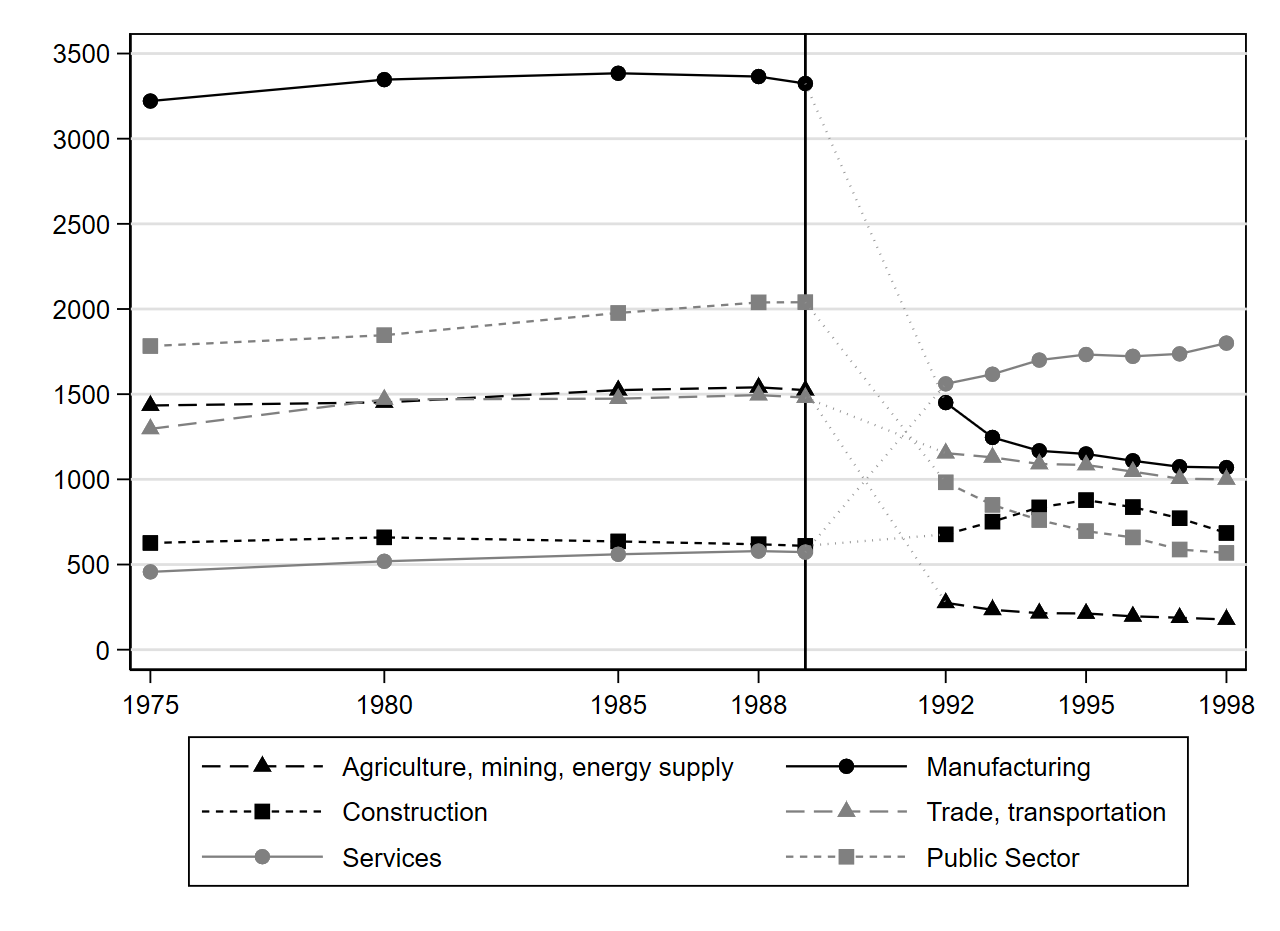
\includegraphics[width=\textwidth]{emp_East.png}
         \caption{East}
         \label{Fig1a}
     \end{subfigure}
     \hfill
     \begin{subfigure}[b]{0.8\textwidth}
         \centering
         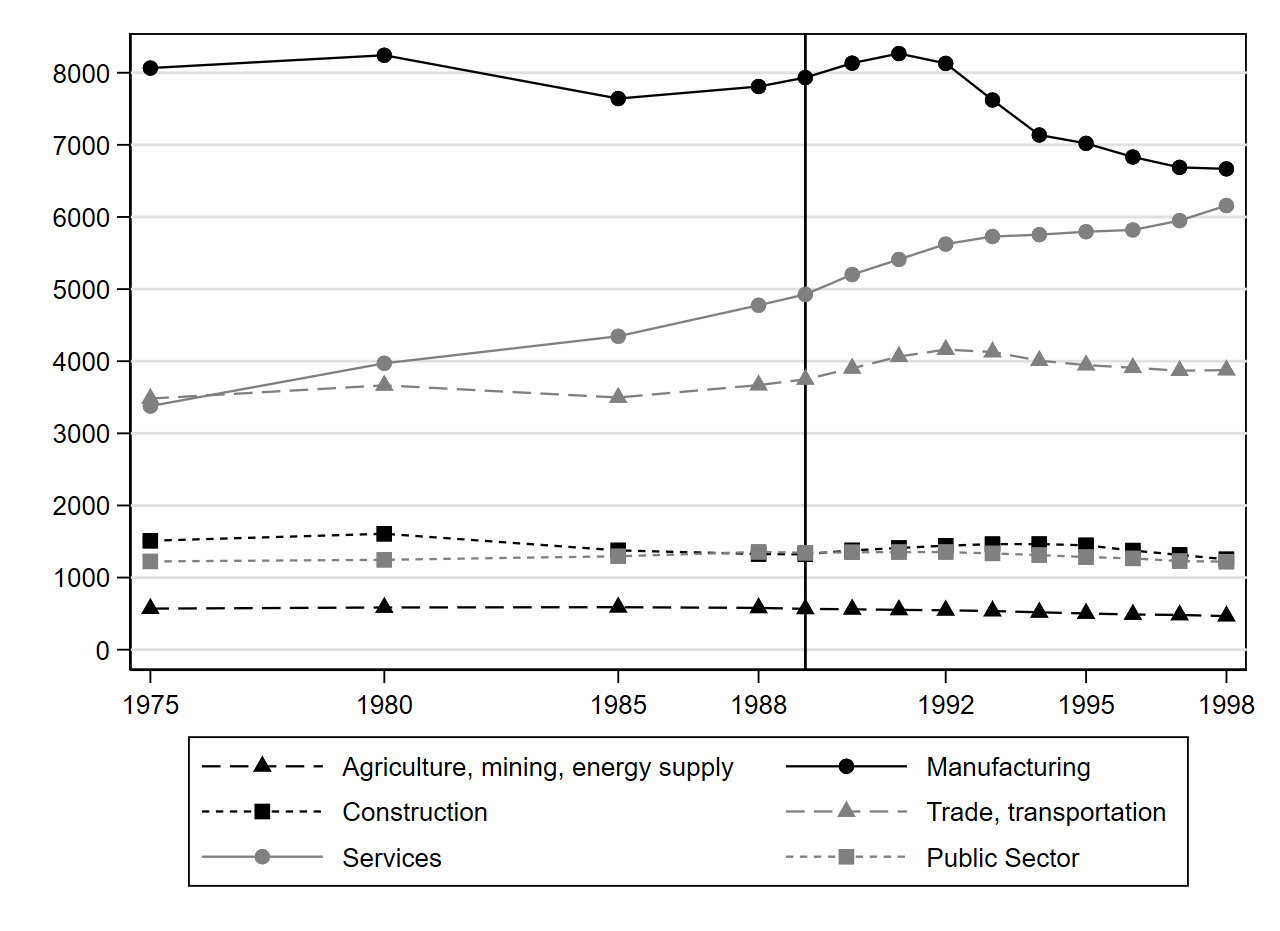
\includegraphics[width=\textwidth]{emp_West.png}
         \caption{West}
         \label{Fig1b}
     \end{subfigure}
     {\footnotesize
    \hspace*{0.1cm}\parbox[h]{\linewidth}{Notes: Y-scale in thousands of workers. The figure corresponds to \cite{FindeisenLeePorzioDauth2021}, Figure~2. The authors generously made the data available for replication. They provide details on the data sources.}}
\end{figure}
%\newpage
%=====================================================================%

The change in paradigm for the East German labor market is also visible in the evolution of unemployment. Unemployment did not officially exist in the GDR, with the right to work being part of the constitution.  Figure \ref{fig2} shows that this changed rapidly after the Wall fell. In 1991, the first year it was officially recorded for East Germany, the unemployment rate among East German men was 8.7\%. With 11.9\%, it was even higher among East German women. It gradually increased for East German men, first relatively slowly, but it accelerated after 1995 and reached 17.5\% in 1998. For East German women, the increase in the unemployment rate was faster during the first half of the 1990s and then remained relatively stable at around 20\%. Throughout the observation period, the unemployment rate among East German women was larger than among East German men.

The change in the unemployment rate in West Germany was much smoother during this period, albeit not constant. In 1988, with 9.4\%, West German women also experienced a relatively high level of unemployment, which declined to 7.0\% in 1991 before increasing even beyond the initial level to 10.2\% in 1998. West German men experienced an unemployment rate of 6.5\% in 1988, which declined to 5.0\% in 1990 before catching up to (and in some years even overtaking) the unemployment rate of West German women. 


The figures demonstrate that the GDR workforce, who had never experienced unemployment or the need for adjustments to structural changes, was suddenly confronted with both these realities on a massive scale, more or less overnight. In this study, I focus on occupational mobility between 1989 and 1992, that is, in the immediate years following the fall of the Berlin Wall, the so-called ``Wende''.

% \vspace{1cm}
%====================================================================%
\begin{figure}[!ht]
    \caption{Evolution of Unemployment in East and West Germany by Gender, 1988--1998}
    \label{fig2}
    \centering
    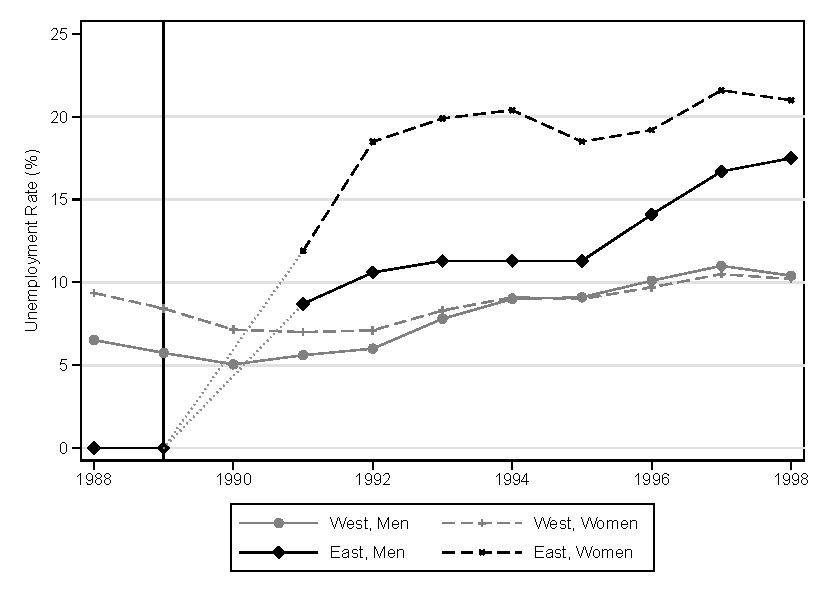
\includegraphics[scale=0.8]{UE_ASO.pdf} 
    \sourcefigure{Federal Employment Agency, various years.}
\end{figure}
%\newpage
%==================================================================%

When investigating occupational mobility in these years and assessing how unusual those years were for the GDR workforce, it is important to understand occupational mobility patterns during GDR times. To the best of my knowledge, the main source of information concerning the rates and patterns of occupational mobility during GDR times comes from the East German Life History Study (EGLHS) of the Max Planck Institute for Human Development and Education in Berlin. \cite{HuininkSolga1994} analyze the pattern of occupational mobility of four cohorts of GDR citizens born in 1929-31, 1939-41, 1951-53, and 1959-61 by comparing their occupational structure at age 30. During GDR times, job mobility could have resulted from modernization and industrialization. However, owing to central planning and state-governed labor force allocation, socialist societies are often characterized as being immobile (a notion that is consistent with the patterns shown in Figure \ref{Fig1a} discussed above). 

\cite{HuininkSolga1994} show, however, that the aggregate figures hide important heterogeneity across birth cohorts. Birth cohorts differed in age when they were subject to the different political and economic developments of the former GDR. Huinink and Solga differentiate three major periods:\footnote{I follow the categorization in \cite{HuininkSolga1994}. More detailed descriptions of the GDR system and its different phases can be found, for example, in \cite{Ritschl1995}.} (1) the period of the revolutionary implementations of the state-socialist system (from the end of World War II to the early 1960s), (2) the period of extensive economic growth connected with attempts at decentralization (the 1960s), and (3) the period of re-centralization of the economy (after Honecker came to power in 1971).

In the first phase, the roots of Nazi Germany were dismantled by introducing new rules and political measures to eliminate the old political, economic, and also bourgeois intellectual elites. These political measures included expropriation, abolishing civil servant status, and denazification. The teachers, lawyers, and civil servants, among other status groups of the previous regime, were ``downgraded'' and replaced by people loyal to the new system. During this period, labor scarcity was a widespread challenge for the GDR. This was not only due to the purging of pre-war personnel and the establishment of a new socialist administration but also because approximately 1.9 million people left the GDR for West Germany. This exodus only ended in 1961 with the construction of the Berlin Wall.\footnote{See, e.g., \cite{BlackLiepmannRemigereauSpitzOener2022}, and studies cited there.} Overall, this period was characterized by general scarcity of labor and resulted in an improvement in the occupational opportunities of men who started from lower levels of qualification, which was consistent with the political goal of creating the GDR as a ``state of workers and farmers''.

The second phase started in the 1960s, and it was characterized by the system's attempt to make the economy more efficient by following a decentralization strategy (the so-called ``Neues \"Okonomisches System, N\"OS, ``New Economic System''). During this period, access to education improved considerably, and the political system ensured a smooth transition from schools to the labor market by requiring and offering everyone a place in the vocational training system. Despite its initial positive effects on economic growth, the N\"OS fell overall short in improving the GDR economy, a fact that led to the third phase.

The third phase is associated with Erich Honecker's coming to power in 1971, which again changed the GDR's economic goals. One of the main measures was the re-centralization of the GDR economy, characterized, among other things, by the establishment of the Kombinate—large state-owned conglomerates covering the majority of an industry's plants. It was also a period in which the opportunities for higher education were reduced, and more generally, the state took an important role in labor allocation.

\cite{HuininkSolga1994} show that the opportunities to improve their occupational position that the earliest birth cohort benefitted from presented themselves to a much smaller degree to those born later, with upward occupational mobility being generally tight to system loyalty displayed by party membership or the taking on of official functions in a pro-party organization. By focusing on the occupational achievements when cohort members were 30 years old, \cite{HuininkSolga1994} show that intra-cohort mobility between the different birth cohorts was very different in the GDR. They do not investigate occupational mobility in the context of the ``Wende,'' which is the main focus of this study.

The cohort-based approach followed by \cite{HuininkSolga1994} is interesting because it allows for comparing GDR and FRG workers in 1989 who are from the same birth cohorts. Methodologically, this comparison allows netting out macro-economic factors that affected the occupational mobility of workers of different ages to a similar degree between 1989 and 1992, independent of whether they lived in the GDR or the FRG in 1989. 

However, it is also interesting to consider the differences and similarities of the different birth cohorts depending on where they were born. Based on \cite{Ritschl1995} and \cite{EichengreenRitschl2009}, I give a brief overview of the differential economic and social environments to which the different cohorts were subjected. 

One striking fact is that the 1929-31 cohort shared the same political and economic environment at birth and early childhood. This cohort was born before World War II (WWII) when Germany was still united. It was born during the early years of the Great Depression (1929-1932), a period of severe economic downturn that deeply affected all regions in Germany.\footnote{See, e.g., \cite{Schnabel2004}.} This cohort was subject to vast economic instability, high unemployment rates, and widespread poverty during their early childhood. The cohort lived under the same political and economic system until WWII ended in 1945 when they were about 15 years old. Then, the macro environment of the GDR and FGR members of this cohort diverged drastically, however, with the division into East and West Germany and the beginning of the Cold War. Those in the East faced a socialist regime under Soviet influence, while those in the West saw the establishment of a democratic state and economic recovery. The West German members of this cohort experienced the period of the  Wirtschaftswunder (Economic Miracle) in West Germany of the 1950s and 1960s when they were of prime working age. Overall, the political and economic environment differed vastly for the GDR and FRG members of the 1929-31 cohort after 1945.

The 1939-41 cohort was born during the early years of World War II. As infants and toddlers, they were exposed to the immediate impacts of the war, including air raids, displacement, and general instability. They were in their early childhood when they experienced the destructive consequences of the war and the division of Germany. Their formative years coincided with the immediate post-war period, characterized by massive reconstruction efforts and economic hardship. West Germany's Wirtschaftswunder began in the late 1940s and accelerated in the 1950s, providing improving living conditions and economic opportunities as they reached adolescence and young adulthood. This cohort benefited from increased access to education, which was a crucial factor in the country's rapid economic recovery. Socialization in this period was also marked by strongly emphasizing democratic principles and rejecting totalitarian ideologies.

Members of the 1951-53 cohort were among the first to be born in the two divided states founded in 1949, the GDR and FRG. Both states underwent a period of significant reconstruction and recovery. In the West, this era is characterized by the booming economy and an expansion of the welfare state, leading to rapid economic growth and rapidly increasing living standards. In East Germany, the members of this cohort grew up in phases (1) and (2) described above. Independent of whether they grew up in the East or the West, because of their early birth, the members experienced all phases of political and economic development from the period of division to reunification. They reached adulthood when the Cold War was the characterizing policy between the East and the West. 

The 1959-61 cohort was born during a period of heightened Cold War tensions. The Berlin Wall, erected in 1961, symbolized the division they were born into, significantly impacting their early years. In West Germany, they experienced a society focused on economic growth and integration with Western Europe and Western countries more generally, while in East Germany, they lived under a socialist regime with a state-controlled economy, limited political freedoms, and strong political and economic connections to the Soviet Union. 


%====================================================================%
\section{Data and Variables}\label{data}
\subsection{Data on GDR Workers}\label{GDRdata}
The novel, individual-level administrative data set on GDR workers used in this study is the result of linking data from the so-called ``Data Fund of Societal Work Power'' of the GDR (``Datenspeicher Gesellschaftliches Arbeitsvermögen (GAV)'' in German), obtained from the Federal Archive in Germany, with the so-called ``Integrated Employment Biographies'' (IEB data). The former provides information on the demographics and labor market characteristics of around 7 million persons in the GDR in 1989, representing the near universe of workers in the GDR. The latter contains the complete employment and earnings histories of all workers covered by the social security system in Germany from 1975 onward. The two data sets were merged on names, exact dates of birth, and gender. The combined data allows for addressing questions regarding mobility across jobs, occupations, and migration decisions after German reunification while also providing labor market information on GDR workers during GDR times.\footnote{A detailed description of the data sources and linkage can be found in \parencite{LiepmannMuller2018}.} 


%====================================================================%
\subsection{Data on FRG Workers}
For information on the cohorts born in the FRG, I rely on the Sample of Integrated Labor Market Biographies (SIAB) of the Institute for Employment Research (IAB). It is a 2\% random sample drawn from the IEB, the database to which the GDR workers were merged, as described above. It provides high-quality information on the labor market trajectory of workers, including information on the occupation, employer, and gross daily wages. In the context of this study, I selected all employed men and women of the relevant birth cohorts in the FRG 1989, including full- and part-time workers (the sample includes about 12\% part-time workers). In contrast to the sample described in \ref{GDRdata}, which includes the near universe of GDR workers, I rely on a 2\% random sample of FRG workers for efficiency reasons. This explains the differences in sample size shown below. 

%====================================================================%
\subsection{Main Variables}

To be able to compare the occupational structure in the two very different economic systems of the GDR and FRG, I use a variant of the so-called Blossfeld occupational categories that categorize occupations into 6 categories, depending on socio-economic status. The six broad categories allow for comparing the occupational structure of two states with very different economic systems. This also allows comparing the results with previous findings in \cite{MayerSolga1994} and \cite{HuininkSolga1994}, among others. Table \ref{tab1} shows the categories. The first category, ``Professional and higher technical, administrative, managerial occupations,'' includes engineers, technicians, managers, and senior government officials. The second category, ``Semiprofessional occupations,'' includes journalists, translators, librarians, and teachers. The third category, ``Skilled workers,'' includes craftsmen, mechanics, bakers, butchers, and brewers. The fourth category, ``Unskilled workers,'' includes assemblers, building laborers, packagers, and dispatchers. The fifth category, ``missing employment information,'' is somewhat of a residual, including, for example, non-agricultural family assistants, trainees, and interns without specified occupations. This category is probably closest to category (4), ``unskilled workers.'' The sixth category, ``non-employed,'' includes non-employed workers.

Regarding occupational mobility between 1989 and 1992, "upward mobility" is defined as moving into a lower numerical category, such as from 3 to 1; ``downward mobility'' is defined as moving into a higher numerical category, such as from 1 to 3. ``Movement to non-employment'' is defined as moving from any non-level 6 category in 1989 to category 6 in 1992. ``Lateral mobility'' is defined as movements between occupations that are in the same category, and ``non-movement'' is defined as staying in the same 2-digit occupation. Note that this classification completely ignores regional mobility. For example, a person who stayed in the same 2-digit occupation is part of the  ``non-movement'' category even though they might have moved from Rostock to Mannheim.

%====================================================================%

\begin{table}[h!]
\caption{Employment Categories}\label{tab1}
\centering
\begin{tabular}{cl}
\toprule
Number & Category \\
\midrule
1 & Professionals, and higher technical, administrative, \\
  & and managerial occupations \\ 
2 & Semiprofessional occupations \\ 
3 & Skilled workers \\ 
4 & Unskilled workers \\
5 & Missing employment information \\ 
6 & Non-employed \\ \bottomrule
\end{tabular}
\end{table}

%==================================================================%

\clearpage
I consider three different levels of education: the low-educated have no vocational training degree, the medium-educated have a degree through the dual system of apprenticeship or a vocational school, and the high-educated have a degree from a university or a technical college. Because of the joint historical roots of the education system in the two parts of Germany, this variable is easy to construct for GDR and FRG workers.



%====================================================================%
\section{The Status Quo in 1989}\label{StatusQuo}

Using information about education and occupational structure, I will first compare the GDR and FRG labor market in 1989, i.e., when the Berlin Wall fell. Table \ref{tab2} shows summary statistics for the 4 birth cohorts (1929-31, 1939-41, 1951-1953, 1959-61) for GDR workers (Panel A) and FRG workers (Panel B) in 1989, separately by gender. It is important to note that, by fixing the year to 1989 and looking at different cohorts, we are comparing demographic groups of different ages in 1989. The oldest cohort was, on average, 60 years old in 1989, the 1939-41 cohort was 49, the 1951-53 cohort was 37, and the 1959-61 cohort was 29 years old in 1989. Differences across cohorts might, therefore, reflect age effects. This is not the case when discussing results for the same birth cohort across demographic groups (men and women in the GDR or FRG), as members of the same birth cohort across groups were of the same age in 1989.\footnote{\cite{HuininkSolga1994} fix the age to 30 when comparing the different cohorts.}

%=======================================================%
%\vspace{1cm}   
\begin{table}[!ht]
\caption{Summary Statistics in 1989}\label{tab2}
\centering
\resizebox{\textwidth}{!}{
\begin{tabular}{lrrrrrrrrrr}
\toprule
\multicolumn{2}{l}{\textbf{Panel A: GDR Workers}} & \multicolumn{9}{c}{\textbf{}}\\ [0.1cm]
\cline{1-11}
 &  &  &  &  &  &  &  &  &  &  \\
\multicolumn{1}{l}{\textbf{}} & \multicolumn{5}{c}{\textbf{Men}} & \multicolumn{5}{c}{\textbf{Women}} \\ [0.3cm]
%\cline{1-11} 
\multicolumn{1}{l}{\textbf{Birth cohort:}} & {\textbf{1929-31}} & \multicolumn{1}{c}{\textbf{1939-41}} & {\textbf{1951-53}} & {\textbf{1959-61}} & \multicolumn{1}{c}{\textbf{all}} & {\textbf{1929-31}} & {\textbf{1939-41}} & {\textbf{1951-53}} & {\textbf{1959-61}} & \multicolumn{1}{c}{\textbf{all}} \\ \midrule
\multicolumn{1}{l}{Share (in\%)} & \multicolumn{10}{c}{} \\ 
... low educated  & {74.5} & {11.4} & {8.4} & {8.1} & {15.9} & {45.6} & {22.8} & {11.0} & {9.6} & 14.9 \\ 
\multicolumn{1}{l}{... medium educated} & {19.3} & {74.6} & {79.5} & {84.4} & {73.4} & {51.1} & {72.4} & {79.2} & {82.4} & 77.7 \\ 
\multicolumn{1}{l}{... higher educated} & {6.2} & {14.0} & {12.1} & {7.4} & {10.6} & {3.3} & {4.9} & {9.8} & {8.0} & 7.4 \\
 ... in occupation group (1)  & {7.8} & {8.5} & {6.5} & {5.1} & {6.8} & {4.7} & {6.8} & {11.7} & {11.8} & 10.0 \\ 
... in occupation group (2)  & {0.9} & {0.6} & {0.4} & {0.3} & {0.5} & {5.4} & {6.4} & {8.2} & {9.2} & 7.9 \\ 
... in occupation group (3)  & {48.6} & {51.0} & {54.3} & {54.1} & {52.7} & {22.2} & {25.7} & {31.3} & {28.7} & 28.5 \\ 
... in occupation group (4) & {29.4} & {27.1} & {26.4} & {25.4} & {26.6} & {35.0} & {40.0} & {35.4} & {38.9} & 38.1 \\
... in occupation group (5)  & {13.3} & {12.9} & {12.3} & {15.2} & {13.5} & {32.6} & {21.1} & {13.3} & {11.4} & 15.5 \\ [0.2cm]
Average Age \\ (Std. Dev.) & {\begin{tabular}[t]{@{}r@{}}58.6\\ (0.75)\end{tabular}} & {\begin{tabular}[t]{@{}r@{}}49.0\\ (0.81)\end{tabular}} & {\begin{tabular}[t]{@{}r@{}}37.0\\ (0.82)\end{tabular}} & {\begin{tabular}[t]{@{}r@{}}29.0\\ (0.82)\end{tabular}} & {\begin{tabular}[t]{@{}r@{}}40.4\\ (9.99)\end{tabular}} & {\begin{tabular}[t]{@{}r@{}}58.8\\ (0.79)\end{tabular}} & {\begin{tabular}[t]{@{}r@{}}49.0\\ (0.81)\end{tabular}} & {\begin{tabular}[t]{@{}r@{}}37.0\\ (0.82)\end{tabular}} & {\begin{tabular}[t]{@{}r@{}}29.0\\ (0.82)\end{tabular}} & \begin{tabular}[t]{@{}r@{}}38.7\\ (8.53)\end{tabular} \\[0.5cm]
\multicolumn{1}{l}{Number of Observations} & {81,137} & {241,047} & {233,329} & {242,806} & {798,319} & {5,777} & {215,961} & {199,821} & {208,266} & 629,825 \\ \bottomrule
 &  &  &  &  &  &  &  &  &  &  \\
 &  &  &  &  &  &  &  &  &  &  \\
\multicolumn{2}{l}{\textbf{Panel B: FRG Workers}} & \multicolumn{9}{c}{\textbf{}}\\ [0.1cm]
\cline{1-11}
 &  &  &  &  &  &  &  &  &  &  \\
\multicolumn{1}{l}{\textbf{}} & \multicolumn{5}{c}{\textbf{Men}} & \multicolumn{5}{c}{\textbf{Women}} \\ [0.3cm]
%\cline{1-11} 
\multicolumn{1}{l}{\textbf{Birth cohort:}} & {\textbf{1929-31}} & {\textbf{1939-41}} & {\textbf{1951-53}} & {\textbf{1959-61}} & \multicolumn{1}{c}{\textbf{all}} & {\textbf{1929-31}} & {\textbf{1939-41}} & {\textbf{1951-53}} & {\textbf{1959-61}} & \multicolumn{1}{c}{\textbf{all}} \\ \midrule
\multicolumn{1}{l}{Share (in\%)} & \multicolumn{10}{c}{} \\
... lower educated  & {62.1} & {25.0} & {18.6} & {21.3} & {27.1} & {88.6} & {39.8} & {31.0} & {40.0} & 42.9 \\ 
\multicolumn{1}{l}{... medium educated} & {32.9} & {67.2} & {68.4} & {68.3} & {63.4} & {10.7} & {58.0} & {63.5} & {53.1} & 52.7 \\ 
\multicolumn{1}{l}{... high educated} & {5.0} & {7.7} & {12.9} & {10.3} & {9.5} & {0.7} & {2.3} & {5.4} & {6.9} & 4.4 \\ 
... in occupation group (1) & {19.5} & {19.8} & {19.2} & {15.5} & {18.3} & {3.3} & {4.3} & {6.5} & {9.6} & 6.5 \\ 
... in occupation group (2) & {1.4} & {1.3} & {2.8} & {2.3} & {2.0} & {6.0} & {6.0} & {9.6} & {13.0} & 9.2 \\ 
... in occupation group (3) & {35.4} & {37.0} & {42.5} & {43.6} & {40.2} & {32.4} & {37.4} & {40.9} & {43.3} & 39.7 \\ 
... in occupation group (4) & {43.8} & {41.9} & {35.5} & {38.6} & {39.5} & {58.3} & {52.2} & {42.9} & {34.1} & 44.7 \\ [0.2cm]
Average Age \\ (Std. Dev.) & {\begin{tabular}[t]{@{}r@{}}58.8\\ (0.80)\end{tabular}} & {\begin{tabular}[t]{@{}r@{}}49.01\\ (0.81)\end{tabular}} & {\begin{tabular}[t]{@{}r@{}}37.0\\ (0.81)\end{tabular}} & {\begin{tabular}[t]{@{}r@{}}29.0\\ (0.82)\end{tabular}} & {\begin{tabular}[t]{@{}r@{}}41.0\\ (10.51)\end{tabular}} & {\begin{tabular}[t]{@{}r@{}}58.8\\ (0.78)\end{tabular}} & {\begin{tabular}[t]{@{}r@{}}49.0\\ (0.81)\end{tabular}} & {\begin{tabular}[t]{@{}r@{}}37.0\\ (0.82)\end{tabular}} & {\begin{tabular}[t]{@{}r@{}}29.0\\ (0.82)\end{tabular}} & \begin{tabular}[t]{@{}r@{}}40.5\\ (10.28)\end{tabular} \\ [0.5cm]
\multicolumn{1}{l}{Number of Observations} & {8,769} & {20,561} & {17,196} & {21,025} & {67,551} & {4,462} & {12,850} & {10,660} & {13261} & 41,233 \\ \bottomrule
\end{tabular}}

\vspace{0.3cm}
\parbox[h]{\linewidth}{\footnotesize{Note: The table shows summary statistics for workers of the German Democratic Republic (GDR) and the Federal Republic of Germany (FRG) in 1989. See Section \ref{data} for details on the data and definition of variables.}}
\end{table}
%\end{landscape}
%\vspace{1cm}

%======================================%

As discussed above, the oldest cohort (born 1929-31) is interesting, as they were born and grew up under the same political and economic system until the end of WWII, when they were about 15 years old. Note surprisingly, in terms of formal education, it is the least educated cohort. 74.5\% of the GDR men of this cohort had low levels of education in 1989, while this figure was considerably lower at 62\% for FRG men of this cohort. In contrast, the share of medium educated was considerably higher for FGR men of this cohort compared to their GDR counterparts. The share of highly educated was quite similar, with 6.2\% for GDR men and 5.0\% for FRG men. 

Regarding women, it is important to note that labor force participation at about 43\% was relatively low in the FRG in 1989, whereas the estimates for the GDR are around 80-90\%. As a result, working women in the FRG were much more selective than in the GDR. Against this background, the differences in formal education are striking between women in the GDR and FRG. While only about 46\% of GDR women in the oldest cohort had low levels of education, this figure was 89\% for FRG women. In addition, 51\% of GDR women had a medium level of education, compared to only 11\% of FRG women. More than 3\% of GDR women in this cohort even had a degree from a university or a technical college.  

For the subsequent cohorts and both genders, the educational structure typical for the German labor market is visible in both groups, with men and women of medium education making up the largest shares. Overall, the across-cohort patterns show that educational upgrading was large for both genders and in both parts of Germany up to 1989. When comparing the two youngest cohorts of GDR workers, the "Honecker" years are also visible, as the educational attainment shifted from high towards medium-educated workers.

The table also shows the distribution of employment across the 5 different occupation groups used in the previous literature and described in Table \ref{tab1}. With about 9\%, the share of ``Professional/Higher technical, administrative, managerial'' occupations (group 1) and ``Semiprofessional'' positions (group 2) among the 1929-31 cohort of GDR men was much lower than the about 21\% among FRG men. Most (about 49\%) of GDR men in this cohort worked as skilled workers (group 3), while this group comprised about 35\% of FRG male workers. The share of unskilled workers in the GDR was about 30\%, and about 13.5\% of workers were not assignable to one of the categories (a detailed look at the occupations suggests, however, that they are closest to the unskilled group). In the FRG, the share of unskilled male workers was about 44\%, comparable to that of GDR workers in occupation groups (4) and (5) combined. 

Regarding women of this oldest cohort in the FRG and GDR, the share in the highest occupational categories is not dramatically different, with about 10\% in the GDR and about 9\% in the FRG. The share of women working as skilled workers is about 10 percentage points higher in the FRG than in the GDR. 58\% of FRG women worked as unskilled workers (group 4), whereas this is only the case for 35\% of GDR female workers. However, the latter increases by 32 percentage points if one counts the relatively high share of GDR female workers who cannot be unambiguously assigned to either of the categories to the unskilled category. 

Looking across cohorts, the younger the women are, the higher the employment share of the two highest occupational categories (groups 1 and 2). Among the GDR female workers born between 1959 and 1961, 21\% worked in these two occupational categories, whereas this was the case for about 23\% of FRG female workers. About 29\% of female GDR workers were employed as skilled workers, compared to more the 43\% of FRG female workers of this cohort. With about 39\%, the share of female GDR workers who worked as unskilled workers was about 5 percentage points higher than for female FRG workers. In addition, about 11\% of GDR women worked in occupation categories (5) that are also closest to the unskilled category. 

Overall, it is striking that GDR women's better educational attainment did not result in higher shares of employment in higher occupational categories (groups 1 to 3), a pattern that also applies to men (but is less pronounced).


%====================================================================%
\section{Occupational Mobility of GDR Workers Between 1989 and 1992}\label{1989to1992}

How did the first years of transition affect the occupational mobility of the different GDR cohorts? To disentangle the effects of the ``Wende'' from the economic effects that Germany was subject to at the beginning of the 1990s and that affected different cohorts in the same way in East and West Germany, I compare the occupational mobility of GDR workers with that of West Germans from the same birth cohort.

Figure \ref{fig3} displays the differences in employment mobility between 1989 and 1992 of GDR and FRG male workers. Differences in upward, lateral downward, movement-to-non-employment, and non-mobility shifts are displayed with one bar representing each type of mobility for each of the four cohorts considered (1929-31, 1939-41, 1951-53, 1959-61) and across all cohorts. As the difference is taken between GDR and FRG male workers, bars above the x-axis indicate a greater share for GDR than FRG, and bars below the x-axis indicate a smaller share for GDR than FRG male workers. The underlying data, separately for GDR and FRG workers by gender, are shown in Table \ref{tab3}.

\pagebreak

Between 1989 and 1992, male GDR workers of the 1929-1931 birth cohort were 5.6 percentage points more likely to move upward than FRG workers of the same cohort (first bar) and 3.7 percentage points more likely to move to an occupation within the same status category (fourth bar from left); however, they were also 3.3 percentage points more likely to move downward, and about 26 percentage points more likely to move into non-employment. The largest difference exists for non-mobility, with FRG male workers of this cohort being 40 percentage points more likely to stay in the same occupation than GDR workers of this cohort.

Regarding men born between 1939 and 1941 (aged 48-50 in 1989), the GDR men were about 25 percentage points more likely to move upward (first bar in the second cluster of bars) and about 20 percentage points more likely to move to occupations within the same status group than FRG men between 1989 and 1992. However, they are also about 17 percentage points more likely to move downward. With a difference of only 1.4 percentage points, GDR and FRG men of this cohort were about equally likely to move to non-employment. The biggest difference, again, is for non-mobility, where FRG workers are about 63 percentage points more likely to stay in the same occupations than GDR workers.

The overall pattern is very similar for men born from 1951 to 1953 and those born from 1959 to 1961, with all mobility categories being larger for GDR workers than FRG workers. Again, the difference in movement to non-employment is small relative to the differences in other categories; again, the FRG workers are much more likely to remain in the same occupation as the GDR workers. In contrast to the high emphasis typically placed on unemployment regarding labor market developments of GDR workers, for all birth cohorts, except for 1929 to 1931, the largest difference between GDR and FRG male workers is occupational mobility versus occupational stability between 1989 and 1992.

Figure \ref{fig4} shows the differences in employment mobility between 1989 and 1992 of GDR and FRG female workers. The pattern for the oldest cohort, born 1929 to 1931, looks quite different for women than for men. Most strikingly, the share of women moving into non-employment is larger among FRG than GDR women by about 32 percentage points. This is not only different from what is observed for men but also compared to the pattern of all other female cohorts. In contrast, the difference in non-mobility is much smaller for this birth cohort. Upward mobility is about 23 percentage points higher, and lateral mobility is about 12 percentage points for GDR than FRG women of this cohort, whereas downward mobility is about 9 percentage points higher.

Looking across female cohorts, upward mobility is always larger than downward mobility, suggesting that the opportunities for occupational upgrading were larger for GDR women between 1989 and 1992 than for FRG women and compared to the risk of downgrading. However, GDR women also had a higher probability of moving into non-employment. Similar to what is observed for men, for all birth cohorts, except for 1929 to 1931, the largest difference between GDR and FRG male workers is occupational mobility versus occupational stability between 1989 and 1992. 

%====================================================================%
\begin{landscape}
    
\begin{figure}[!ht]
    \caption{\textbf Distribution of East-West Differences in Occupational Shifts between 1989 and 1992 for Selected Birth Cohorts, Men}\label{fig3}
%    \vspace{-0.5cm}
    \begin{center}
    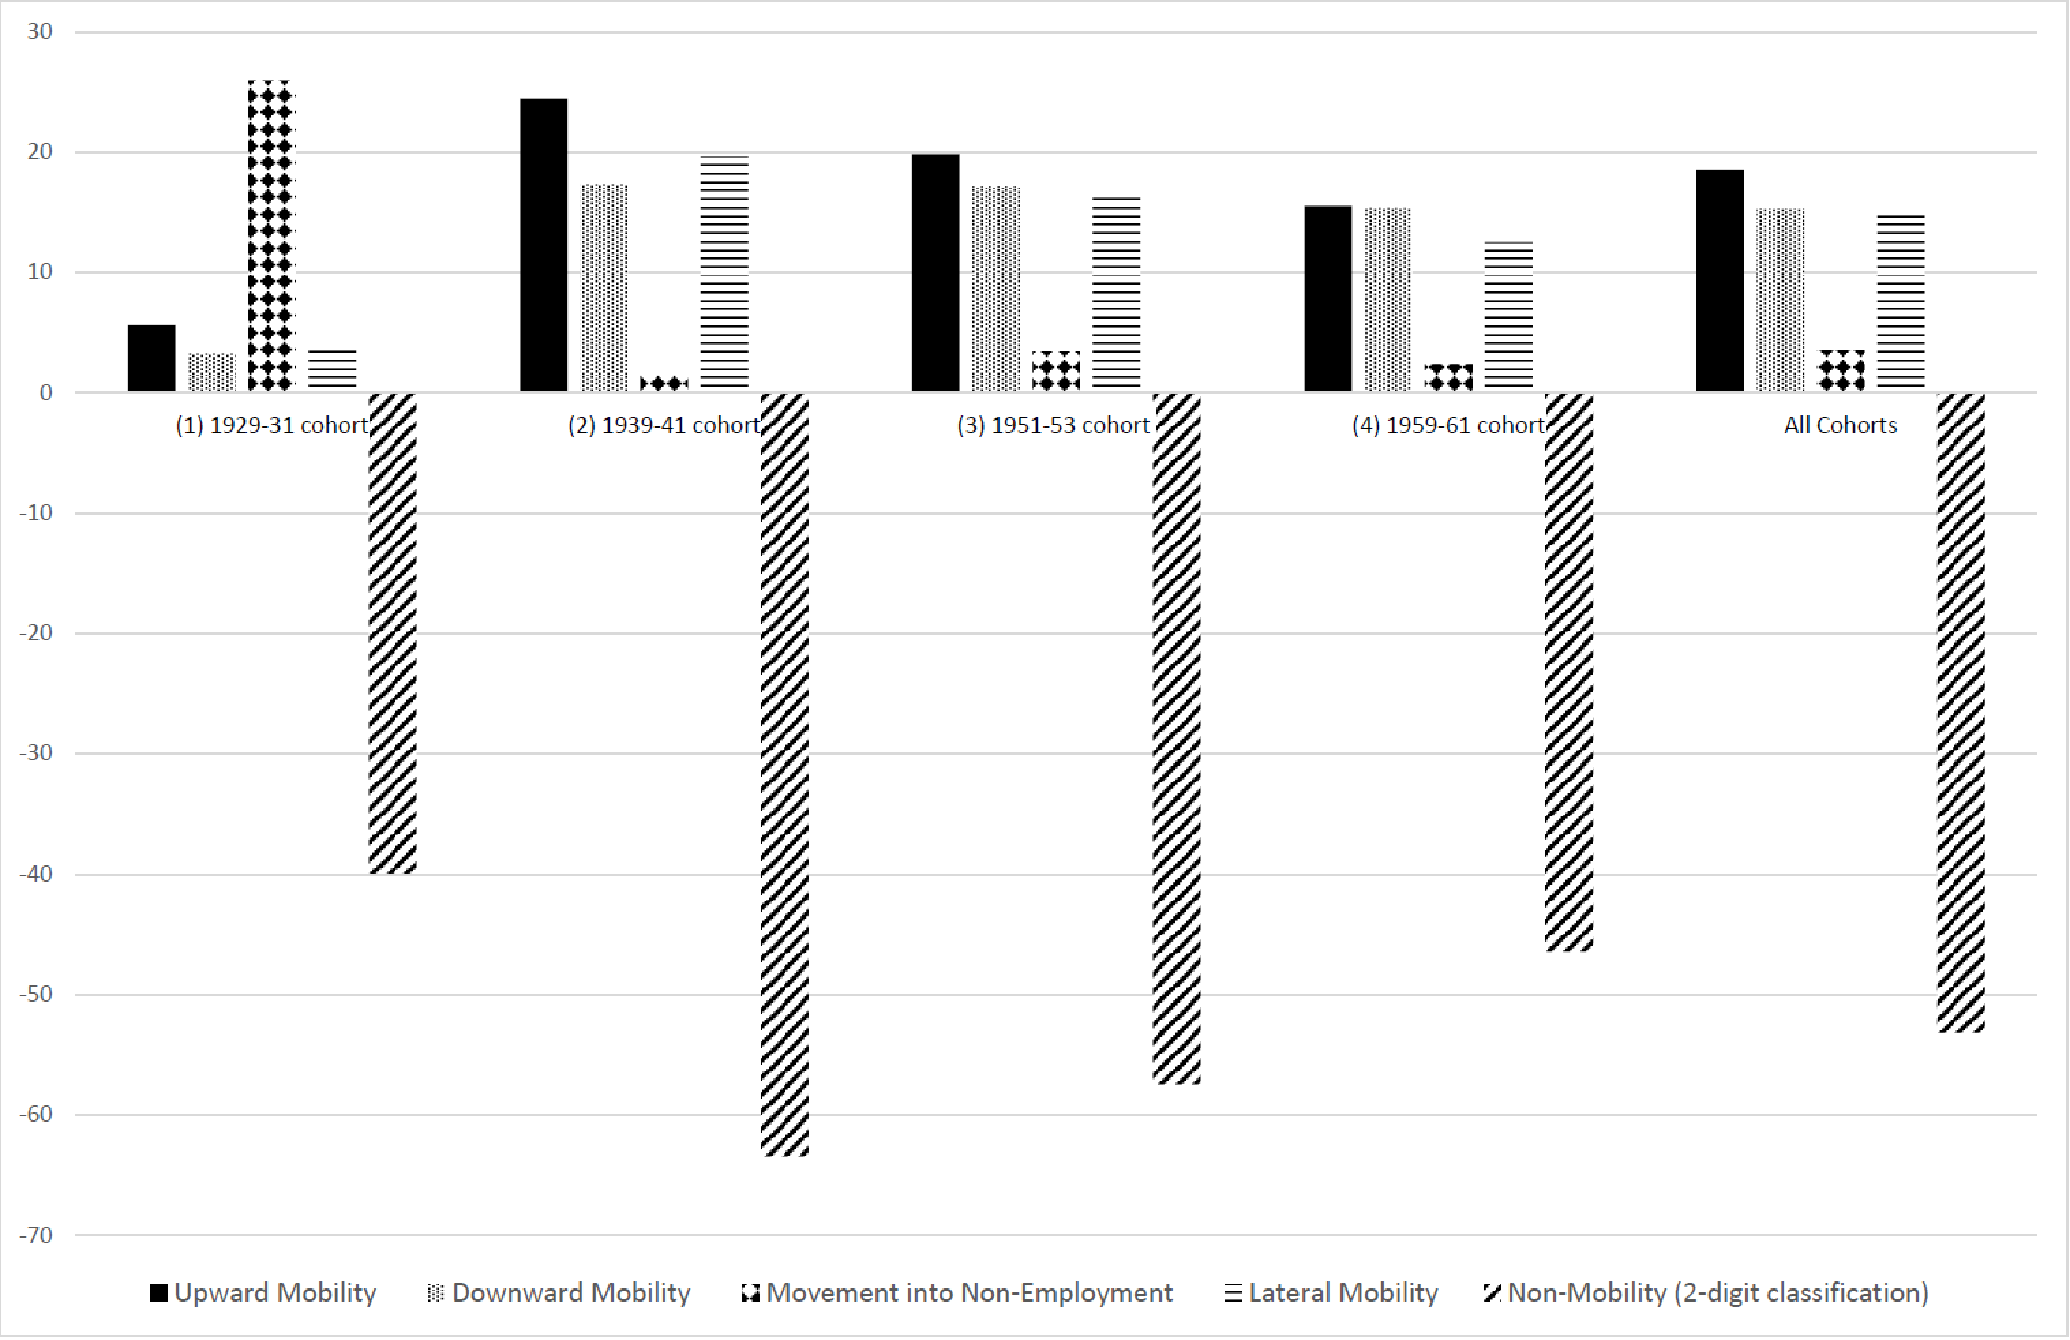
\includegraphics[width=.8\linewidth]{East_vs_West_Men.pdf}
    \vspace{-3.8cm}
    {\footnotesize
    \hspace*{0.1cm}\parbox[h]{\linewidth}{Notes: The figure shows the differences in the shares of occupational mobility of GDR and FRG male workers between 1989 and 1992, separately by birth cohort and overall. ``Upward mobility" is defined as moving into a lower numerical category, such as from 3 to 1 (see Table \ref{tab1}); ``downward mobility'' is defined as moving into a higher numerical category, such as from 1 to 3. ``Movement to non-employment'' is defined as moving from any non-level 6 category in 1989 to category 6 in 1992. ``Lateral mobility'' is defined as movements between occupations that are in the same category, and ``non-movement'' is defined as staying in the same 2-digit occupation.}}
    \end{center}
\end{figure}
\end{landscape}


%====================================================================%
\begin{landscape}
    
\begin{figure}[!ht]
    \caption{\textbf Distribution of East-West Differences in Occupational Shifts between 1989 and 1992 for Selected Birth Cohorts, Women}\label{fig4}
%    \vspace{-0.5cm}
    \begin{center}
    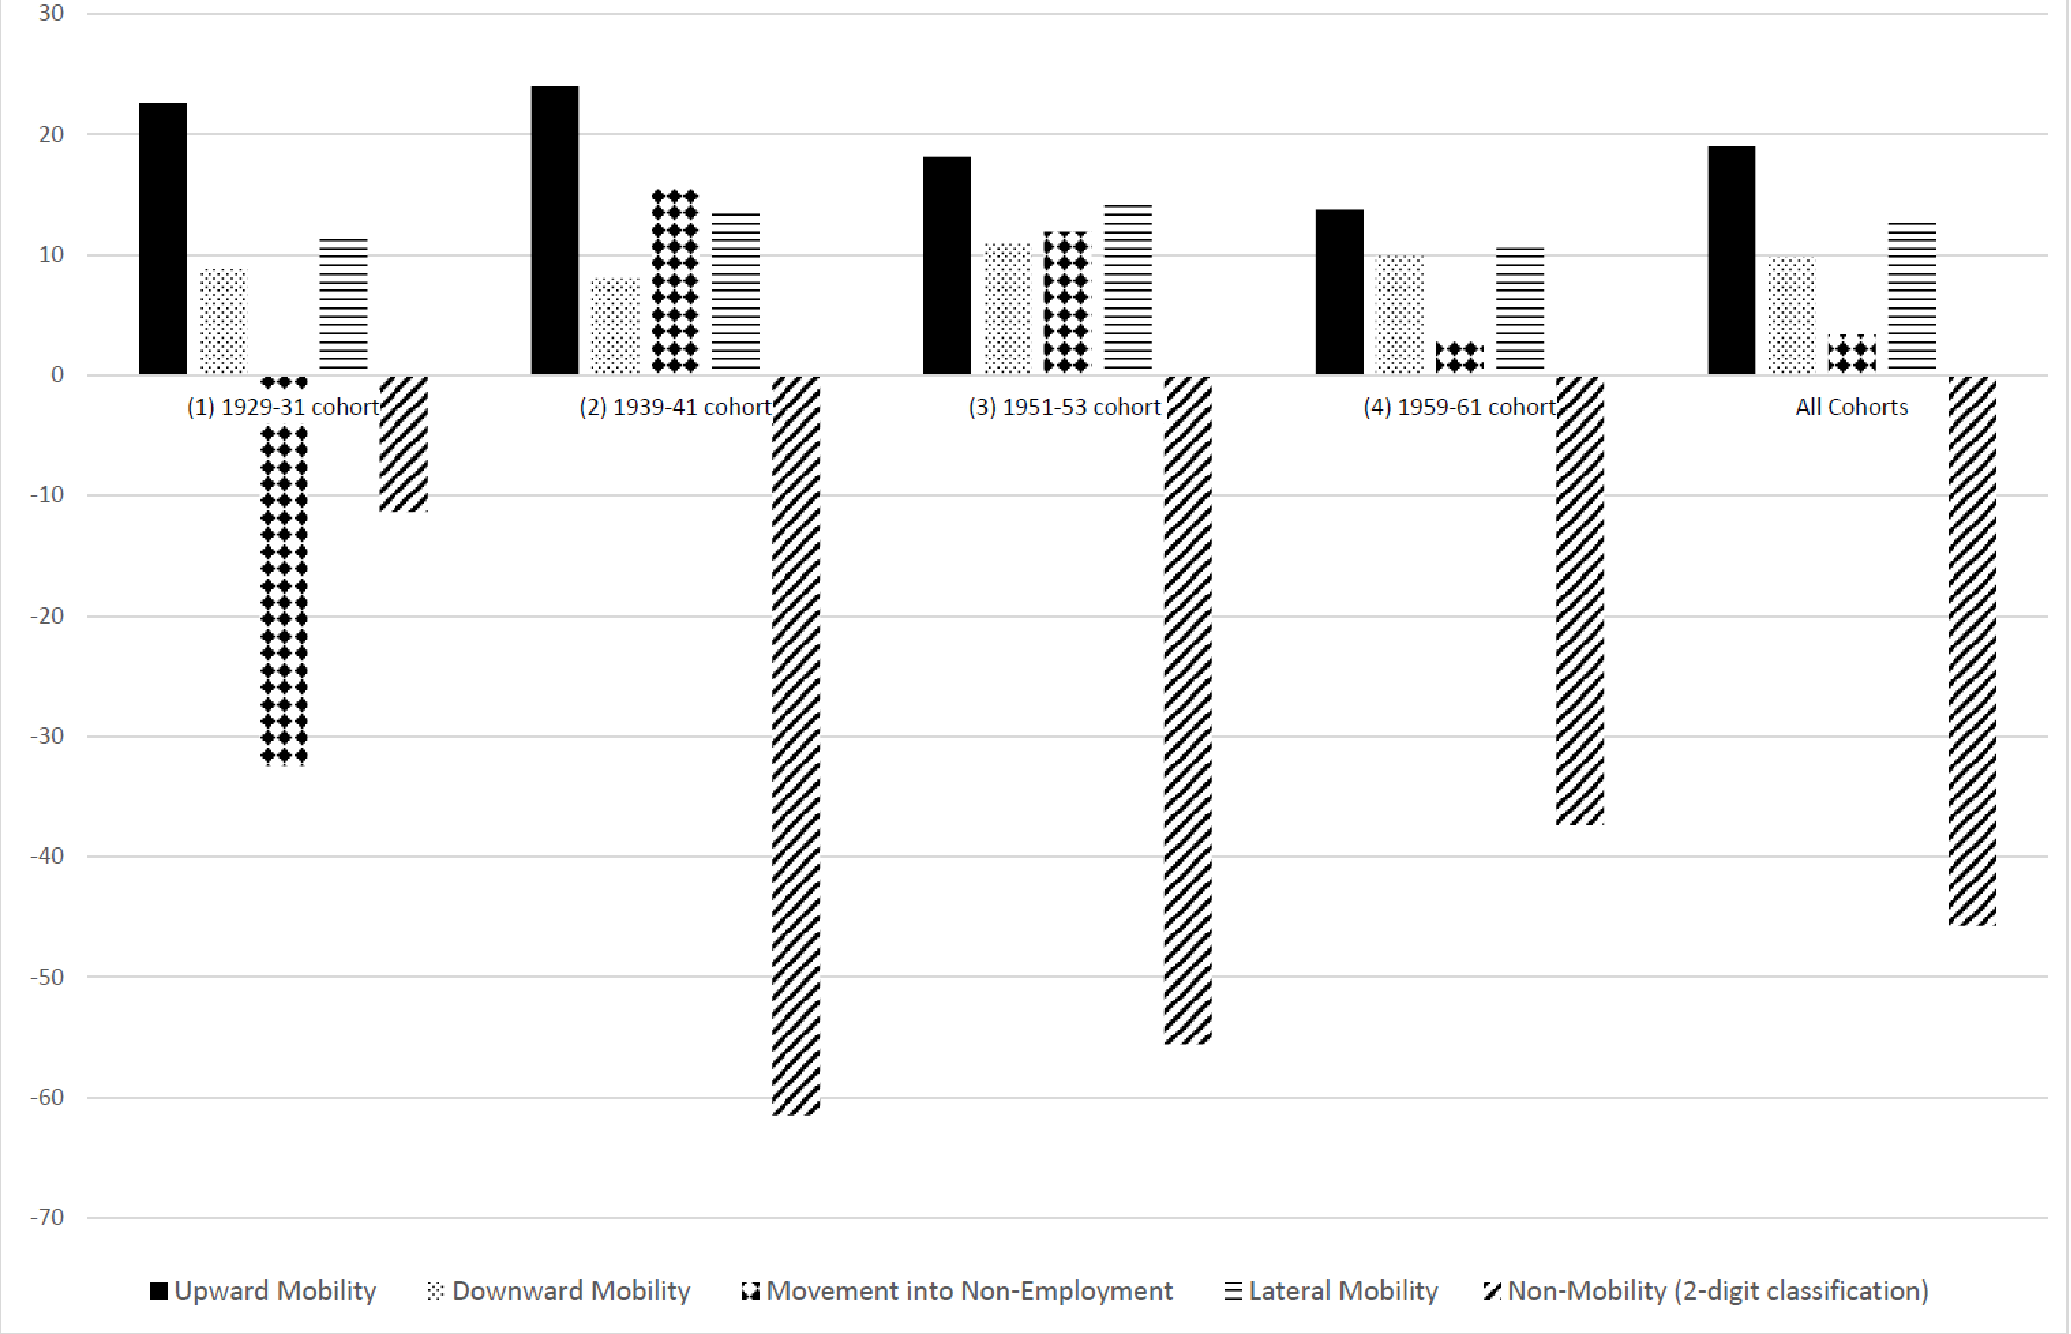
\includegraphics[width=.8\linewidth]{East_vs_West_Women.pdf}
    \vspace{-3.8cm}
    {\footnotesize
    \hspace*{0.1cm}\parbox[h]{\linewidth}{Notes: The figure shows the differences in the shares of occupational mobility of GDR and FRG female workers between 1989 and 1992, separately by birth cohort and overall. ``Upward mobility" is defined as moving into a lower numerical category, such as from 3 to 1 (see Table \ref{tab1}); ``downward mobility'' is defined as moving into a higher numerical category, such as from 1 to 3. ``Movement to non-employment'' is defined as moving from any non-level 6 category in 1989 to category 6 in 1992. ``Lateral mobility'' is defined as movements between occupations that are in the same category, and ``non-movement'' is defined as staying in the same 2-digit occupation.}}
    \end{center}
\end{figure}
\end{landscape}

%---------------------------------------------------------%
\begin{landscape}
\begin{table}[]
\centering
\caption{Occupational Mobility between 1989 and 1992}\label{tab3}
% \vspace{-0.2cm}
\resizebox{12cm}{!}{%
\begin{tabular}{lll*5{r}}
\hline
\multicolumn{1}{r}{} & \multicolumn{1}{r}{\textbf{Sex}} & \multicolumn{1}{r}{\textbf{Cohort}} & \multicolumn{1}{r}{\textbf{Upward Mobility}} & \multicolumn{1}{r}{\textbf{Downward Mobility}} & \multicolumn{1}{r}{\textbf{\begin{tabular}[t]{@{}r@{}}Movement into \\ Non-Employment\end{tabular}}} & \multicolumn{1}{r}{\textbf{\begin{tabular}[t]{@{}r@{}}Lateral Mobility \end{tabular}}} & \textbf{\begin{tabular}[t]{@{}r@{}}Non-Mobility \\ (2-digit classification)\end{tabular}} \\ \hline
\multicolumn{1}{r}{\multirow{10}{*}{\textbf{GDR Workers}}} & \multicolumn{1}{r}{\multirow{5}{*}{Men}} & \multicolumn{1}{l}{(1) 1929-31 cohort} & \multicolumn{1}{r}{7.7} & \multicolumn{1}{r}{3.7} & \multicolumn{1}{r}{80.2} & \multicolumn{1}{r}{4.7} & 3.6 \\ \cline{3-8} 
\multicolumn{1}{r}{} & \multicolumn{1}{r}{} & \multicolumn{1}{r}{(2) 1939-41 cohort} & \multicolumn{1}{r}{26.8} & \multicolumn{1}{r}{19.2} & \multicolumn{1}{r}{14.1} & \multicolumn{1}{r}{23.3} & 16.4 \\ \cline{3-8} 
\multicolumn{1}{r}{} & \multicolumn{1}{r}{} & \multicolumn{1}{r}{(3) 1951-53 cohort} & \multicolumn{1}{r}{24.1} & \multicolumn{1}{r}{20.1} & \multicolumn{1}{r}{15.0} & \multicolumn{1}{r}{22.0} & 18.5 \\ \cline{3-8} 
\multicolumn{1}{r}{} & \multicolumn{1}{r}{} & \multicolumn{1}{r}{(4) 1959-61 cohort} & \multicolumn{1}{r}{21.9} & \multicolumn{1}{r}{19.5} & \multicolumn{1}{r}{16.2} & \multicolumn{1}{r}{21.0} & 21.2 \\ \cline{3-8} 
\multicolumn{1}{r}{} & \multicolumn{1}{r}{} & \multicolumn{1}{r}{All Cohorts} & \multicolumn{1}{r}{22.6} & \multicolumn{1}{r}{18.0} & \multicolumn{1}{r}{21.7} & \multicolumn{1}{r}{20.4} & 17.2 \\ \cline{2-8} 
\multicolumn{1}{r}{} & \multicolumn{1}{r}{\multirow{5}{*}{Women}} & \multicolumn{1}{r}{(1) 1929-31 cohort} & \multicolumn{1}{r}{23.6} & \multicolumn{1}{r}{8.8} & \multicolumn{1}{r}{49.1} & \multicolumn{1}{r}{11.6} & 6.2 \\ \cline{3-8} 
\multicolumn{1}{r}{} & \multicolumn{1}{r}{} & \multicolumn{1}{r}{(2) 1939-41 cohort} & \multicolumn{1}{r}{26.5} & \multicolumn{1}{r}{9.6} & \multicolumn{1}{r}{31.6} & \multicolumn{1}{r}{16.4} & 15.6 \\ \cline{3-8} 
\multicolumn{1}{r}{} & \multicolumn{1}{r}{} & \multicolumn{1}{r}{(3) 1951-53 cohort} & \multicolumn{1}{r}{22.4} & \multicolumn{1}{r}{13.6} & \multicolumn{1}{r}{28.0} & \multicolumn{1}{r}{18.6} & 17.3 \\ \cline{3-8} 
\multicolumn{1}{r}{} & \multicolumn{1}{r}{} & \multicolumn{1}{r}{(4) 1959-61 cohort} & \multicolumn{1}{r}{18.2} & \multicolumn{1}{r}{12.8} & \multicolumn{1}{r}{34.6} & \multicolumn{1}{r}{15.6} & 18.7 \\ \cline{3-8} 
\multicolumn{1}{r}{} & \multicolumn{1}{r}{} & \multicolumn{1}{r}{All Cohorts} & \multicolumn{1}{r}{22.4} & \multicolumn{1}{r}{11.9} & \multicolumn{1}{r}{31.6} & \multicolumn{1}{r}{16.8} & 17.1 \\ \hline
\multicolumn{1}{r}{\multirow{10}{*}{\textbf{FRG Workers}}} & \multicolumn{1}{r}{\multirow{5}{*}{Men}} & \multicolumn{1}{r}{(1) 1929-31 cohort} & \multicolumn{1}{r}{2.1} & \multicolumn{1}{r}{0.5} & \multicolumn{1}{r}{54.3} & \multicolumn{1}{r}{1.0} & 43.5 \\ \cline{3-8} 
\multicolumn{1}{r}{} & \multicolumn{1}{r}{} & \multicolumn{1}{r}{(2) 1939-41 cohort} & \multicolumn{1}{r}{2.3} & \multicolumn{1}{r}{1.9} & \multicolumn{1}{r}{12.7} & \multicolumn{1}{r}{3.5} & 79.8 \\ \cline{3-8} 
\multicolumn{1}{r}{} & \multicolumn{1}{r}{} & \multicolumn{1}{r}{(3) 1951-53 cohort} & \multicolumn{1}{r}{4.3} & \multicolumn{1}{r}{3.0} & \multicolumn{1}{r}{11.6} & \multicolumn{1}{r}{5.4} & 76.0 \\ \cline{3-8} 
\multicolumn{1}{r}{} & \multicolumn{1}{r}{} & \multicolumn{1}{r}{(4) 1959-61 cohort} & \multicolumn{1}{r}{6.4} & \multicolumn{1}{r}{4.1} & \multicolumn{1}{r}{13.8} & \multicolumn{1}{r}{8.5} & 67.6 \\ \cline{3-8} 
\multicolumn{1}{r}{} & \multicolumn{1}{r}{} & \multicolumn{1}{r}{All Cohorts} & \multicolumn{1}{r}{4.1} & \multicolumn{1}{r}{2.7} & \multicolumn{1}{r}{18.2} & \multicolumn{1}{r}{5.2} & 70.3 \\ \cline{2-8} 
\multicolumn{1}{r}{} & \multicolumn{1}{r}{\multirow{5}{*}{Women}} & \multicolumn{1}{r}{(1) 1929-31 cohort} & \multicolumn{1}{r}{1.0} & \multicolumn{1}{r}{0.0} & \multicolumn{1}{r}{81.5} & \multicolumn{1}{r}{0.0} & 17.5 \\ \cline{3-8} 
\multicolumn{1}{r}{} & \multicolumn{1}{r}{} & \multicolumn{1}{r}{(2) 1939-41 cohort} & \multicolumn{1}{r}{2.5} & \multicolumn{1}{r}{1.6} & \multicolumn{1}{r}{16.1} & \multicolumn{1}{r}{2.8} & 77.1 \\ \cline{3-8} 
\multicolumn{1}{r}{} & \multicolumn{1}{r}{} & \multicolumn{1}{r}{(3) 1951-53 cohort} & \multicolumn{1}{r}{4.2} & \multicolumn{1}{r}{2.7} & \multicolumn{1}{r}{16.1} & \multicolumn{1}{r}{4.4} & 72.8 \\ \cline{3-8} 
\multicolumn{1}{r}{} & \multicolumn{1}{r}{} & \multicolumn{1}{r}{(4) 1959-61 cohort} & \multicolumn{1}{r}{4.4} & \multicolumn{1}{r}{2.9} & \multicolumn{1}{r}{31.8} & \multicolumn{1}{r}{5.0} & 56.1 \\ \cline{3-8} 
\multicolumn{1}{r}{} & \multicolumn{1}{r}{} & \multicolumn{1}{r}{All Cohorts} & \multicolumn{1}{r}{3.4} & \multicolumn{1}{r}{2.1} & \multicolumn{1}{r}{28.2} & \multicolumn{1}{r}{3.6} & 62.8 \\ \hline
\multicolumn{8}{c}{\multirow{2}{*}{\textbf{GDR - FRG Differences}}} \\
\multicolumn{8}{c}{} \\ \hline
\multicolumn{1}{r}{\multirow{5}{*}{\textbf{GDR - FRG}}} & \multicolumn{1}{r}{\multirow{5}{*}{Men}} & \multicolumn{1}{r}{(1) 1929-31 cohort} & \multicolumn{1}{r}{5.6} & \multicolumn{1}{r}{3.3} & \multicolumn{1}{r}{25.9} & \multicolumn{1}{r}{3.7} & -39.9 \\ \cline{3-8} 
\multicolumn{1}{r}{} & \multicolumn{1}{r}{} & \multicolumn{1}{r}{(2) 1939-41 cohort} & \multicolumn{1}{r}{24.5} & \multicolumn{1}{r}{17.3} & \multicolumn{1}{r}{1.4} & \multicolumn{1}{r}{19.8} & -63.4 \\ \cline{3-8} 
\multicolumn{1}{r}{} & \multicolumn{1}{r}{} & \multicolumn{1}{r}{(3) 1951-53 cohort} & \multicolumn{1}{r}{19.8} & \multicolumn{1}{r}{17.1} & \multicolumn{1}{r}{3.4} & \multicolumn{1}{r}{16.6} & -57.4 \\ \cline{3-8} 
\multicolumn{1}{r}{} & \multicolumn{1}{r}{} & \multicolumn{1}{r}{(4) 1959-61 cohort} & \multicolumn{1}{r}{15.5} & \multicolumn{1}{r}{15.3} & \multicolumn{1}{r}{2.4} & \multicolumn{1}{r}{12.5} & -46.4 \\ \cline{3-8} 
\multicolumn{1}{r}{} & \multicolumn{1}{r}{} & \multicolumn{1}{r}{All Cohorts} & \multicolumn{1}{r}{18.5} & \multicolumn{1}{r}{15.3} & \multicolumn{1}{r}{3.6} & \multicolumn{1}{r}{15.1} & -53.1 \\ \hline
\multicolumn{1}{r}{\multirow{5}{*}{\textbf{GDR - FRG}}} & \multicolumn{1}{r}{\multirow{5}{*}{Women}} & \multicolumn{1}{r}{(1) 1929-31 cohort} & \multicolumn{1}{r}{22.6} & \multicolumn{1}{r}{8.8} & \multicolumn{1}{r}{-32.4} & \multicolumn{1}{r}{11.6} & -11.3 \\ \cline{3-8} 
\multicolumn{1}{r}{} & \multicolumn{1}{r}{} & \multicolumn{1}{r}{(2) 1939-41 cohort} & \multicolumn{1}{r}{24.0} & \multicolumn{1}{r}{8.1} & \multicolumn{1}{r}{15.4} & \multicolumn{1}{r}{13.6} & -61.5 \\ \cline{3-8} 
\multicolumn{1}{r}{} & \multicolumn{1}{r}{} & \multicolumn{1}{r}{(3) 1951-53 cohort} & \multicolumn{1}{r}{18.2} & \multicolumn{1}{r}{11.0} & \multicolumn{1}{r}{11.9} & \multicolumn{1}{r}{14.2} & -55.5 \\ \cline{3-8} 
\multicolumn{1}{r}{} & \multicolumn{1}{r}{} & \multicolumn{1}{r}{(4) 1959-61 cohort} & \multicolumn{1}{r}{13.8} & \multicolumn{1}{r}{10.0} & \multicolumn{1}{r}{2.8} & \multicolumn{1}{r}{10.6} & -37.3 \\ \cline{3-8} 
\multicolumn{1}{r}{} & \multicolumn{1}{r}{} & \multicolumn{1}{r}{All Cohorts} & \multicolumn{1}{r}{19.0} & \multicolumn{1}{r}{9.8} & \multicolumn{1}{r}{3.4} & \multicolumn{1}{r}{13.1} & -45.7 \\ \hline
\end{tabular}}

\vspace{0.3cm}
\parbox[h]{\linewidth}{\footnotesize{Note: The table shows summary statistics for workers of the German Democratic Republic (GDR) and the Federal Republic of Germany (FRG) in 1989 by birth cohort. See Section \ref{data} for details on the data and definition of variables. Each row shows the share (in\%) of workers of a specific cohort in the respective category. The 7.7, for example, in row 1 for male GDR workers indicates that 7.7\% of male GDR workers born between 1929 and 1931 experienced upward occupational mobility between 1989 and 1992. For each row, the figures across columns sum to 100\%. The figures in the second part of the table ``GDR - FRG differences'' are the basis for Figures \ref{fig3} and \ref{fig4}.}}
%\end{center}
\end{table}
\end{landscape}



%====================================================================%
\section{Conclusion}\label{Concl}

In this brief article, I present descriptive evidence on occupational mobility during German reunification. I use novel data linking administrative labor market information of German Democratic Republic (GDR) workers before and after reunification. This unique data includes the same individuals' information from both systems.

The analyses reveal pronounced differences in the occupational structure of employment in the GDR and FRG in 1989. Despite higher levels of formal education among GDR men and women, professional and semi-professional occupations among GDR workers in 1989 were underrepresented compared to the structure in the FRG, reflecting the differences in the sector composition in the two parts of Germany.

Comparing GDR workers' patterns with those of Federal Republic of Germany (FRG) workers from the same birth cohort, the results reveal diverse patterns of occupational mobility, including upgrading and downgrading. GDR workers generally showed much higher mobility dynamics. The oldest cohort's (aged 58-60 in 1989) transition to non-employment, driving the aggregate patterns, reflects the extensive early retirement schemes in both parts of Germany.

\begingroup
\setlength{\emergencystretch}{3em}
\printbibliography
\endgroup

% \newpage

% %====================================================================%
% {\Large\bf References}

% \begin{itemize}
%   \item[] Akerlof, George, Andrew Rose, Janet Yellen, and Helga Hessenius (1991). East Germany in from the
% Cold: The Economic Aftermath of Currency Union. Brookings Papers on Economic Activity 22 (1),
% 1–106.
%  \item[] Alesina, Alberto, and Nicola Fuchs-Schündeln (2007, September). Good-bye Lenin (or Not?): The Effect
% of Communism on People’s Preferences. American Economic Review 97 (4), 1507–1528.
%  \item[] Black, Sandra E., Hannah Liepmann, Camille Remigereau, and Alexandra Spitz-Oener (2022). Govern-
% ment aid and child refugees’ economic success later in life: Evidence from post-WWII GDR refugees.
% Labour Economics 75, 102099.
%  \item[] Börsch-Supran, Axel, and Peter Schmidt (2001). Early Retirement in East and West Germany, pp.
% 83–102. Springer.
%  \item[] Burda, Michael C., and Jennifer Hunt (2001). From reunification to economic integration: Productivity
% and the labor market in Eastern Germany. Brookings Papers on Economic Activity 2001 (2), 1–92.
%  \item[] Eichengreen, Barry, and Albrecht Ritschl (2009). Understanding West German economic growth in the
% 1950s. Cliometrica 3, 191–219.
%  \item[] Emmler, Julian, and Bernd Fitzenberger (2020). The Role of Unemployment and Job Change When
% Estimating the Returns to Migration. IZA Discussion Paper (13740).
%  \item[] Findeisen, Sebastian, Sang Yoon (Tim) Lee, Tommaso Porzio, and Wolfgang Dauth (2021). Transforming
% Institutions: Labor Reallocation and Wage Growth in a Reunified Germany. Working paper.
%  \item[] Fuchs-Schündeln, Nicola, and Rima Izem (2012). Explaining the low labor productivity in East Germany
% - A spatial analysis. Journal of Comparative Economics 40 (1), 1–21.
%  \item[] Fuchs-Schündeln, Nicola, and Matthias Schündeln (2009). Who stays, who goes, who returns? East-West
% migration within Germany since reunification. Economics of Transition 17 (4), 703–738.
%  \item[] Gruenert, Holle (1996). Das Beschäftigungssystem der DDR. In B. Lutz, H. M. Nickel, R. Schmidt, and
% A. Sorge (Eds.), Arbeit, Arbeitsmarkt und Betriebe. Berichte der Kommission für die Erforschung des
% sozialen und politischen Wandels in den neuen Bundesländern e.V. (KSPW), pp. 17–68. Verlag für
% Sozialwissenschaften.
%  \item[] Hoene, Bernd (1991). Labor market realities in Eastern Germany. Challenge 34 (4), 17–22.
%  \item[] Huinink, Johannes, and Heike Solga (1994). Occupational Opportunities in the GDR: A Privilege of the
% Older Generations? Zeitschrift für Soziologie 23 (3), 237–253.
%  \item[] Hunt, Jennifer (2006). Staunching emigration from east Germany: Age and the determinants of migration.
% Journal of the European Economic Association 4 (5), 1014–1037.
%  \item[] Liepmann, Hannah, and Dana Müller (2018). A Proposed Data Set for Analyzing the Labor Market
% Trajectories of East Germans around Reunification. FDZ-Method Report 3.
%  \item[] Lutz, Burkart, Hildegard Maria Nickel, Rudi Schmidt, and Arndt Sorge (Eds.) (1996). Arbeit, Arbeits-
% markt und Betriebe, Volume 1 of Berichte zum sozialen und politischen Wandel in Ostdeutschland.
% Opladen: Leske u. Budrich.
% 19
% \item[] Mayer, Karl Ulrich, and Heike Solga (1994). Mobilität und Legitimität: zum Vergleich der Chancen-
% strukturen in der alten DDR und der alten BRD oder: Haben Mobilitätschancen zu Stabilität und
% Zusammenbruch der DDR beigetragen? ; Ralf Dahrendorf zum 65. Geburtstag. Kölner Zeitschrift für
% Soziologie und Sozialpsychologie 46 (2), 193–208.
% \item[] Prantl, Susanne, and Alexandra Spitz-Oener (2009). How does entry regulation influence entry into
% self-employment and occupational mobility? Economics of Transition 17 (4), 769–802.
% \item[] Prantl, Susanne, and Alexandra Spitz-Oener (2020). The Impact of Immigration on Competing Natives’
% Wages: Evidence from German Reunification. The Review of Economics and Statistics 102 (1), 79–97.
% \item[] Ritschl, Albrecht (1995). Aufstieg und Niedergang der Wirtschaft der DDR: Ein Zahlenbild 1945-1989.
% Jahrbuch für Wirtschaftsgeschichte/Economic History Yearbook 36 (2), 11–46.
% \item[] Schnabel, Isabel (2004). The German Twin Crisis of 1931. The Journal of Economic History 64 (3),
% 822–871.
% \item[] Stauder, Johannes (2018). (Why) have women left East Germany more frequently than men? Heidelberger
% Jahrbücher Online 3, 73–97.

% \end{itemize}

    \end{refsection}

\end{Article} 
% %\graphicspath{{}}

\selectlanguage{french}

\begin{Article}[Titre=Minimax regret et jeu de demande 11-20,
Auteur={Gisèle Umbhauer\thanks{BETA, Université de Strasbourg. \emph{Correspondance:}
61 avenue de la Forêt Noire, 67085 Strasbourg Cedex, France. \emph{Courriel:} \href{mailto:umbhauer@unistra.fr}{umbhauer@unistra.fr}}}]

\label{UmbhauerFR}

\remerciements{Je remercie deux rapporteurs, ainsi que Jalal El Ouardighi et Bernardo Garcia-Pola pour leurs commentaires constructifs. Je remercie
également les étudiants en troisième année de licence de la Faculté des
sciences économiques et de gestion de l'Université de Strasbourg
(année universitaire 2021-2022), qui ont joué le jeu de demande 11-20.}

\begin{resume}
Le jeu de demande 11-20 d'Arad et Rubinstein stimule naturellement un
comportement conforme au raisonnement de niveau-\emph{k}. Nous montrons,
dans une version généralisée de ce jeu, que le minimax regret joue
également un rôle significatif dans le comportement induit et que la
stratégie mixte de minimax regret mime le raisonnement de
niveau-\emph{k}, dès lors que le nombre de joueurs de niveau-\emph{k}
dans une population chute avec \emph{k}. Nous montrons également qu'il
existe, pour cette famille de jeux, un lien original entre la stratégie
mixte de minimax regret et l'équilibre de Nash en stratégies mixtes, et
nous comparons les paiements obtenus avec les deux concepts.    
\end{resume}

\titrearticleENG{Minimax regret in the 11-20 money request game}

\begin{resumeENG}
Arad and Rubinstein's 11-20 money request game nicely triggers
level-\emph{k} reasoning. We show, in a general class of money-request
games, that mixed-strategy minimax regret plays a significant role too,
and that it mimics level-\emph{k} reasoning, at least if the number of
level-\emph{k} players in a population is supposed to decrease in
\emph{k}. We also show, in this class of games, an original link between
the minimax regret probability distribution and the mixed-strategy Nash
equilibrium distribution, and we compare the payoffs obtained with both
concepts.
\end{resumeENG}

\motscles{minimax regret en stratégies mixtes, raisonnement de
niveau-\emph{k}, jeu de demande 11-20, équilibre de Nash}

\keywords{mixed minimax regret, level-\emph{k} reasoning,
money-request game, Nash equilibrium}

\jelcode{C72}

\newpage

\begin{refsection}[UmbhauerFR]  

\section{INTRODUCTION}

\textcite{arad2012} ont présenté leur jeu de demande 11-20
comme le jeu qui stimule spontanément un raisonnement de
niveau-\emph{k}. Dans ce jeu à deux joueurs, chaque joueur est appelé à
demander un montant monétaire, entier naturel allant de 11 à 20. Chaque
joueur reçoit le montant qu'il demande et obtient un bonus --~montant
additionnel~-- de 20 si sa demande est juste inférieure d'une unité à la
demande de l'autre joueur.

Arad et Rubinstein ont raison, en partie du moins, d'arguer que leur jeu
(appelé <<~jeu 11-20/bonus 20~>> par la suite) est bien conçu pour étudier le
raisonnement de niveau-\emph{k}. En effet, premièrement, tout est fait
dans ce jeu pour stimuler ce type de raisonnement. Le raisonnement de
niveau-0, point d'ancrage des itérations, fait consensus~: il consiste à
jouer 20, car en jouant 20, un joueur s'assure le gain 20, qui est le
paiement maximin du jeu, ici inhabituellement élevé. Aussi un joueur qui
ne souhaite pas mener de raisonnement sophistiqué jouera sûrement 20, et
20 est donc le montant naturel pour débuter les itérations de
niveau-\emph{k}. Il s'ensuit que demander 19 est le comportement naturel
de niveau-1 (car 19 est la meilleure réponse à 20), que demander 18 est
le comportement naturel de niveau-2 (car 18 est la meilleure réponse à
19), et ainsi de suite. De plus, le conflit entre les deux acteurs est
limité, au sens où chacun obtient ce qu'il demande indépendamment du
montant demandé par l'autre; la volonté de jouer une meilleure réponse
ne devrait donc pas être entravée par des considérations sociales.
Deuxièmement, la suite des itérations de niveau-\emph{k} ne peut pas
être obtenue par d'autres types de raisonnement usuels. Il n'y a pas de
stratégie dominée dans ce jeu, aussi la dominance itérée n'a pas
d'impact; elle ne peut donc conduire au même résultat que le
raisonnement de niveau-\emph{k} (contrairement à ce qui se passe dans le
jeu de devinette -- concours de beauté -- voir \textcite{nagel1995}). Il n'y a
pas non plus d'équilibre de Nash en stratégies pures qui serait le
comportement vers lequel converge le raisonnement de niveau-\emph{k}
(contrairement au jeu de devinette). Troisièmement, le jeu est très
simple et ne demande (presque) pas de compétences cognitives pour
progresser dans la séquence des itérations. Contrairement aux jeux de
devinette, où chaque itération additionnelle nécessite le calcul d'une
nouvelle moyenne, ici chaque nouvelle itération exige uniquement de
diminuer le montant demandé de 1; la simplicité de ce calcul explique
notamment qu'une version réduite du jeu d'Arad et Rubinstein ait été
utilisée dans des expériences avec de très jeunes enfants, âgés de 5 ans
et plus (voir \textcite{fe2022}). Pour toutes ces raisons, le jeu
11-20/bonus20 semble être effectivement apte à tester le raisonnement de
niveau-\emph{k}, et plus spécifiquement la profondeur de raisonnement
des acteurs (c'est-à-dire le nombre \emph{k} d'itérations qu'ils
choisissent de mener).

Ce jeu a donné lieu à de nombreuses expériences (parmi elles \textcite{arad2012}, \textcite{lindner2013}, \textcite{goeree2018}, \textcite{li2018}, \textcite{alosferrer2021}). Certaines de ces expériences ont apporté des éclairages sur la profondeur de raisonnement et le temps de décision. Ainsi, \textcite{lindner2013} ont cherché si une contrainte temporelle pouvait
stimuler un comportement plus proche de l'équilibre de Nash\linebreak\par
\pagebreak\noindent en
stratégies mixtes et \textcite{alosferrer2021} ont étudié
le lien entre temps de décision et profondeur de raisonnement.

Toutefois le jeu d'Arad et Rubinstein a une propriété non partagée par
d'autres jeux testant le raisonnement de niveau-\emph{k}, tels les jeux
de devinette usuels. Comme cela a été observé par \textcite{li2018},
alors que les paiements des joueurs dans les jeux de devinette sont
toujours identiques (1 pour le gagnant et 0 pour les perdants), le
paiement obtenu par un joueur dans le jeu 11-20/bonus20 dépend fortement
du nombre choisi. Les gains minimaux et maximaux d'un joueur sont
croissants en fonction du montant demandé (à l'exception de 20) : un
joueur gagne au moins 19 et au plus 39 en jouant 19 alors qu'il gagne au
moins 11 et au plus 31 en choisissant 11. Ce fait peut stimuler des
traits comportementaux différents du raisonnement de niveau-\emph{k}. \textcite{li2018} ont mentionné l'aversion au risque, qui conduit
effectivement les joueurs à jouer des grands nombres plus souvent, et
\textcite{goeree2018} ont montré que la connaissance commune d'un
bruit dans le comportement mène également à jouer plus fréquemment des
grands nombres.

\enlargethispage{\baselineskip}

Dans cet article, nous arguons que le minimax regret est une autre façon
d'approcher le jeu. Le minimax regret (MR par la suite) est un concept
bien connu en théorie de la décision où il est associé à l'aversion
contre l'ambiguïté (et remonte à \textcite{savage1951} et \textcite{niehans1948}), mais il n'a été introduit que plus récemment en théorie des
jeux par \textcite{linhart1989}, \textcite{renou2010} et \textcite{halpern2012}. 
Le jeu 11-20/bonus20 comprend en effet une forte incertitude stratégique : chaque montant est rationalisable selon le concept de \textcolor{red}{Pearce [1984]} (car chaque demande \emph{x} de 11 à 19 est une meilleure réponse à la demande \(x + 1\), et 20 est la meilleure réponse à 11). D'où il est difficile d'anticiper le comportement de
l'autre joueur, et chaque décision peut générer un regret. Il découle
qu'il peut être plus raisonnable de minimiser les regrets générés plutôt
que d'essayer de répondre optimalement à une stratégie qui ne peut être
anticipée. De plus, la stratégie mixte à laquelle conduit le MR s'avère être
en accord avec la distribution de comportements générée par le
raisonnement de niveau-\emph{k}, jusqu'à une certaine profondeur de
raisonnement, si on suppose que le nombre de joueurs de niveau-\emph{k}
dans une population décroît avec \emph{k}. Ainsi le comportement issu du
raisonnement de niveau-\emph{k} peut également être obtenu en minimisant
le regret, et ce malgré que la minimisation du regret traduise une
philosophie comportementale totalement différente. \textcite{garciapola2020} a déjà observé un lien entre raisonnement de niveau-1 et MR
en stratégies pures itéré. Mais le MR en stratégies pures ne prend en
compte que les regrets maximaux, ce qui est très restrictif. Le MR en
stratégies mixtes exploite mieux tous les regrets du jeu et conduit
ainsi à un lien plus intéressant entre MR et raisonnement de
niveau-\emph{k}.

L'objectif de l'article est d'analyser ce lien ainsi que le lien entre
MR en stratégies mixtes et équilibre de Nash en stratégies mixtes, dans
une version généralisée du jeu d'Arad et Rubinstein. Nous comparons
également les gains obtenus avec le MR et l'équilibre de Nash. Enfin
nous étudions l'impact du MR dans des variantes du jeu 11-20/bonus20,
développées par \textcite{arad2012} et \textcite{goeree2018}, et nous commentons quelques traits comportementaux issus d'une expérience en classe.

En section~\ref{section:Jeu de demande exp en classe}, nous commençons par étudier brièvement comment 410~étudiants ont joué le jeu 11-20/bonus20 dans une expérience en classe menée à l'Université de Strasbourg. Cette expérience illustrera les
résultats obtenus dans les sections ultérieures. En section~\ref{section:Minimax Reg dans le jeu} nous
déterminons le comportement associé au MR en stratégies mixtes dans le
jeu 11-20/bonus20, avant d'établir ce comportement dans la version
généralisée de ce jeu. Nous montrons que la stratégie mixte qui minimise
le regret (<<~MR stratégie mixte~>> par la suite) mime une distribution
compatible avec un raisonnement de niveau-\emph{k}, quand le pourcentage
de joueurs de niveau-\emph{k} décroît avec la profondeur de
raisonnement. En section~\ref{section:Minimax Reg équilibre} nous étudions le lien original existant entre la MR stratégie mixte et l'équilibre de Nash en stratégies mixtes dans la version généralisée du jeu d'Arad et Rubinstein et nous commentons
les gains obtenus avec les deux concepts. En section~\ref{section:Commentaires sur MR} nous étudions l'impact du MR dans des variantes du jeu 11-20/bonus20. En section~\ref{section:Conclusion Umbhauer_fr} nous concluons sur des traits comportementaux observés lors de l'expérience en classe menée à Strasbourg.

\section{JEU DE DEMANDE 11-20 AVEC BONUS 20,\\ UNE EXPÉRIENCE EN CLASSE}
\label{section:Jeu de demande exp en classe}

L'expérience en classe s'est déroulée lors d'un cours de théorie des
jeux avec des étudiants en troisième année de licence de la Faculté des
sciences économiques et de gestion de l'Université de Strasbourg, durant
l'année universitaire 2021-2022. Au total 410~étudiants ont participé à
l'expérience. Les étudiants étaient homogènes en âge (entre 19 et 21~ans) et en domaine d'études (économie et gestion). Comme il est usuel
dans les expériences en classe, aucune rémunération monétaire n'a été
versée aux étudiants mais leur participation a été stimulée par une
rémunération en note de participation entrant dans la note finale à
l'examen de fin de semestre. L'expérience est un jeu joué en
\emph{one-shot}. Le jeu a été expliqué et plusieurs exemples ont été
donnés avant le début de l'expérience, pour s'assurer que les règles du
jeu soient comprises\footnote{Pour faciliter la compréhension du jeu,
  les montants étaient exprimés en euros (dans l'expérience
  d'AR [2012] les montants étaient en shekels).}. Les étudiants ont
joué le jeu avant de connaître les concepts de dominance et d'équilibre
de Nash (EN par la suite), mais ils connaissaient la notion de jeu sous
forme normale matricielle. Aussi, au moment de leur choix, ils avaient
sous leurs yeux la matrice du jeu 11-20/bonus20 (matrice~1)\footnote{Pour
  faciliter la lecture de la matrice, les gains du joueur~1 étaient
  écrits en rouge. Usuellement, dans les autres expériences portant sur
  le jeu 11-20/bonus20, les joueurs n'ont pas la matrice de paiements à
  disposition au moment du choix. Le fait de disposer de cette matrice
  peut avoir un impact sur les choix, dans la mesure où cela rend plus
  aisée la comparaison entre le gain personnel et le gain de
  l'adversaire (on reviendra sur ce fait en section~\ref{section:Conclusion Umbhauer_fr}).}.

Les étudiants devaient répondre à la question suivante :
\og{}Imaginez que vous êtes le joueur~1 et que vous êtes confronté à
un autre étudiant, le joueur~2, choisi aléatoirement dans
l'amphithéâtre. Quel montant demandez-vous~?\fg{} Ils étaient invités à
justifier leur choix par écrit.

\begin{table}[h!]
\centering
Matrice 1 : jeu 11-20/bonus20
\label{matrice1}
\resizebox{.85\linewidth}{!}{
\begin{tabular}{lc | c*{9}{c} | }
\multicolumn{12}{c}{P12} \tabularnewline % fusionner 12 cellules, centrer (c)
 & \multicolumn{1}{c}{} & 11 & 12 & 13 & 14 & 15 & 16 & 17 & 18 & 19 & \multicolumn{1}{c}{20} \tabularnewline
\cline{3-12}
& 11 & (11,11) & (31,12) & (11,13) & (11,14) & (11,15) & (11,16) &
(11,17) & (11,18) & (11,19) & (11,20) \tabularnewline
& 12 & (12,31) & (12,12) & (32,13) & (12,14) & (12,15) & (12,16) &
(12,17) & (12,18) & (12,19) & (12,20) \tabularnewline
& 13 & (13,11) & (13,32) & (13,13) & (33,14) & (13,15) & (13,16) &
(13,17) & (13,18) & (13,19) & (13,20) \tabularnewline
& 14 & (14,11) & (14,12) & (14,33) & (14,14) & (34,15) & (14,16) &
(14,17) & (14,18) & (14,19) & (14,20) \tabularnewline
Pl1 & 15 & (15,11) & (15,12) & (15,13) & (15,34) & (15,15) & (35,16) &
(15,17) & (15,18) & (15,19) & (15,20) \tabularnewline
& 16 & (16,11) & (16,12) & (16,13) & (16,14) & (16,35) & (16,16) &
(36,17) & (16,18) & (16,19) & (16,20) \tabularnewline
& 17 & (17,11) & (17,12) & (17,13) & (17,14) & (17,15) & (17,36) &
(17,17) & (37,18) & (17,19) & (17,20) \tabularnewline
& 18 & (18,11) & (18,12) & (18,13) & (18,14) & (18,15) & (18,16) &
(18,37) & (18,18) & (38,19) & (18,20) \tabularnewline
& 19 & (19,11) & (19,12) & (19,13) & (19,14) & (19,15) & (19,16) &
(19,17) & (19,38) & (19,19) & (39,20) \tabularnewline
& 20 & (20,11) & (20,12) & (20,13) & (20,14) & (20,15) & (20,16) &
(20,17) & (20,18) & (20,39) & (20,20) \tabularnewline
\cline{3-12}
\end{tabular}}
\end{table}

Les résultats de l'expérience sont donnés dans le tableau 1 et dans la
figure 1. Le tableau 1 précise également les résultats obtenus dans les
expériences d'\textcite{arad2012} (AR par la suite) et \textcite{li2018} (LR par la suite), ainsi que l'EN symétrique\footnote{Le jeu 11-20/bonus20 a d'autres EN en stratégies mixtes asymétriques, mais tous partagent la propriété que les probabilités attribuées aux montants joués décroissent avec le montant, avec une possible
  exception pour le plus bas montant joué. L'un de ces équilibres est
  tel que l'un des joueurs joue 13, 15, 17 et 19, respectivement avec
  les probabilités 8/20, 6/20, 4/20 et 2/20, alors que l'autre joueur
  joue 12, 14, 16, 18 et 20, respectivement avec les probabilités 2/20,
  7,5/20, 5,5/20, 3,5/20 et 1,5/20.} en stratégies mixtes et la MR
stratégie mixte qui sera calculée en section~\ref{section:Minimax Reg dans le jeu}.

\begin{table}[h!]
\caption{Quelques expériences du jeu 11-20/bonus20, ainsi que
  l'équilibre de Nash symétrique en stratégies mixtes et la stratégie
  mixte qui minimise le regret}\label{tabl1}
\centering
\resizebox{\linewidth}{!}{
\begin{tabular}{l    *{10}{D{6mm}}}
\toprule
Montant demandé & \centering 11 & \centering 12 & \centering 13 & \centering 14 & \centering 15 & \centering 16 & \centering 17 & \centering 18 & \centering 19 & \centering 20 \tabularnewline
\midrule
Expérience de Strasbourg (\%) & 8,3 & 0,7 & 2 & 4,4 & 4,9 & 5,9 & 14,9 &
17,5 & 28 & 13,4 \tabularnewline
Expérience AR (\%) & 4 & 0 & 3 & 6 & 1 & 6 & 32 & 30 & 12 & 6 \tabularnewline
Expérience LR (\%) & 0 & 0 & 0 & 7.3 & 1 & 4.2 & 19,8 & 37,5 & 26 &
4.2 \tabularnewline
EN symétrique (\%) & 0 & 0 & 0 & 0 & 25 & 25 & 20 & 15 & 10 & 5 \tabularnewline
MR stratégie mixte (\%) & 0 & 0 & 0 & 0 & 5 & 10 & 15 & 20 & 25 & 25 \tabularnewline
\bottomrule
\end{tabular}}
\end{table}


\begin{figure}[h]
    \centering
    \caption{Expérience en classe de l’université de Strasbourg (pourcentages) (2021/2022)}
    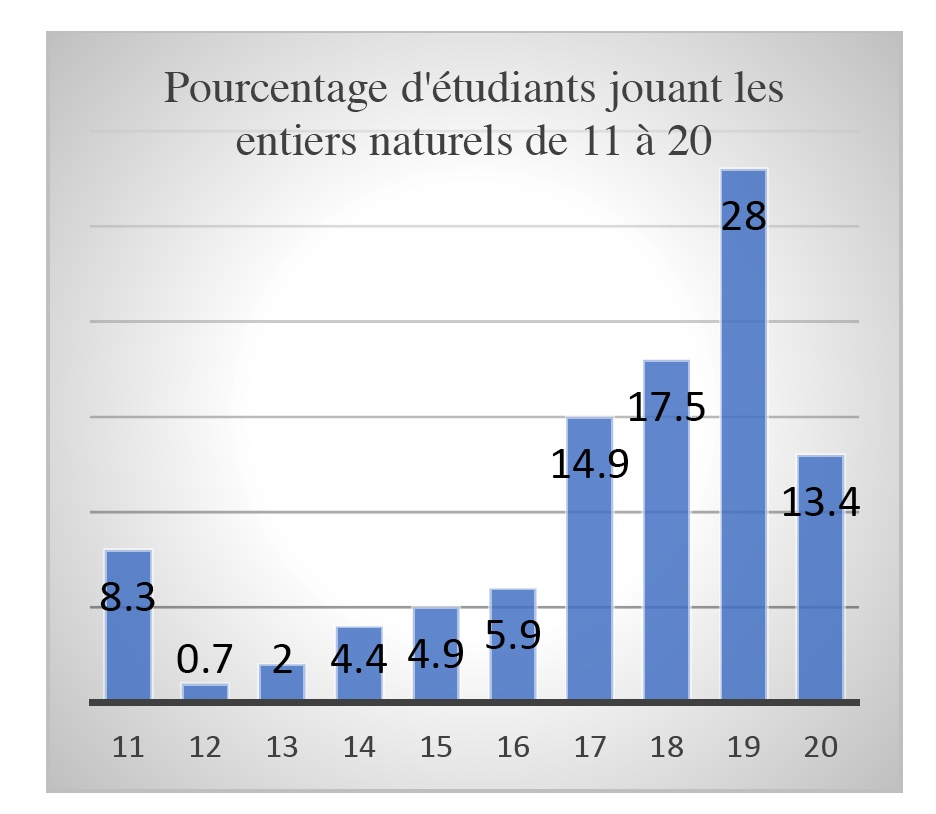
\includegraphics[height=6cm]{Articles-bons-a-composer/02_Umbhauer/02_Umbhauer_fr_Figures/02_Umbhauer_fr_figure-1.jpeg}
\end{figure}

La figure 1 est en accord avec un fait fréquemment observé dans les jeux
stimulant des raisonnements de niveau-\emph{k}, notamment les jeux de
devinette (concours de beauté), à savoir que le pourcentage de joueurs
de niveau-\emph{k} décroît avec \emph{k}, la profondeur de raisonnement
(\(k > 0\)). Ainsi 28~\% des étudiants de Strasbourg choisissent 19 (le
montant de niveau-1), 17,5~\% d'entre eux jouent 18 (raisonnement de
niveau-2), 14,9~\% d'entre eux jouent 17 (raisonnement de niveau-3) et
ainsi de suite jusqu'à 12 (voir le tableau 1). Seule l'observation que 8,3~\%
des étudiants jouent 11 n'est pas en accord avec ce fait. Cette
décroissance régulière de 19 à 12 n'est pas toujours observée dans les
autres expériences portant sur le jeu 11-20/bonus20. Ainsi 19 n'est pas
toujours le mode statistique de la distribution : c'est le cas chez \textcolor{red}{Alos-Ferrer et Buckenmaier [2018]}, mais chez AR [2012] c'est 17 et chez \textcite{lindner2013}, \textcite{goeree2018} et \textcite{li2018} c'est 18.
Plus généralement les distributions de comportements varient selon les
études\footnote{Par exemple un test du khi-deux, même restreint aux
  distributions sur les entiers de 16 à 19, montre que la distribution
  d'AR (108 joueurs) est significativement différente de celle obtenue
  dans l'expérience en classe de Strasbourg (410~joueurs) ($p<0,001$). La distribution de Strasbourg est plus proche de celle
  obtenue par \textcolor{red}{Alos-Ferrer et
  Buckenmaier [2018]} (128~joueurs), si on
  exclut les joueurs jouant 17, très peu nombreux chez Alos-Ferrer et
  Buckenmaier: les deux distributions, restreintes aux entiers 16, 18,
  19 et 20, ne sont pas significativement différentes ($p=0,14$).}
mais elles partagent toutes la propriété que les pourcentages
décroissent de 18 (ou 17 chez AR) à 14 au moins (de toute façon les
pourcentages d'acteurs demandant 11, 12, 13 sont généralement faibles).
Et toutes les distributions empiriques diffèrent profondément de l'EN
symétrique en stratégies mixtes (la valeur \emph{p} des tests du
khi-deux peut être approximée par 0).

\section{MINIMAX REGRET DANS LE JEU DE DEMANDE 11-T\\ AVEC BONUS B}
\label{section:Minimax Reg dans le jeu}

Nous abordons maintenant le MR et appliquons ce concept à une version
généralisée du jeu d'Arad et Rubinstein, le jeu 11-T/bonus\emph{B,} \emph{i.e.}
le jeu de demande 11-\emph{T} avec bonus \emph{B}, où
\(B \geq T > 11 + n\), \emph{n} étant l'entier naturel défini par :
\(n(n + 1)/2\  \leq B < (n + 1)(n + 2)/2\) (\(B = T = 20\) et \(n = 5\)
dans le jeu d'Arad et Rubinstein).

Le concept de MR est bien connu en théorie de la décision avec
incertitude et remonte à \textcite{savage1951} et \textcite{niehans1948}. Un
agent économique, lorsqu'il ne lui est pas possible d'anticiper le futur
état du monde (état de la Nature) peut opter pour une décision qui
minimise son regret, à savoir la différence entre le gain généré par sa
décision et le gain obtenu avec la meilleure décision dans l'état du
monde finalement réalisé. Le MR peut notamment partiellement expliquer
le comportement des acteurs dans le paradoxe d'\textcite{ellsberg1961}. Dans
un jeu, les joueurs ne sont pas confrontés à la Nature ou à des loteries
--~du moins pas exclusivement~-- mais à d'autres joueurs. Ils peuvent
toutefois être confrontés à une forte incertitude stratégique au sens où
il peut s'avérer difficile, pour de multiples raisons, d'anticiper
comment les autres acteurs vont jouer. Dans un tel contexte, minimiser
le regret peut s'avérer plus optimal que de jouer une meilleure réponse
à un profil de stratégies complètement inconnu.

Dans un jeu, le concept de MR en stratégies pures est défini ainsi. Soit
un jeu sous forme normale avec \emph{N} joueurs \emph{i}, des ensembles
de stratégies pures \emph{S\textsubscript{i}} et des fonctions d'utilité
\emph{u\textsubscript{i}, i} de 1 à \emph{N\textsubscript{~}}; le regret
du joueur \emph{i} lorsqu'il joue la stratégie pure\({\ \ s}_{i}\ \)et
que les autres joueurs jouent les stratégies pures
$s_{-i}$ est
\(r_{i}(s_{i},~s_{-i}) = \max_{\sigma_{i} \in S_{i}}{u_{i}\left( \sigma_{i},~s_{-i} \right) - u_{i}\left( s_{i},s_{- i} \right)}\).
Le regret maximal lié à \emph{s\textsubscript{i}} est\linebreak
\(R_{i}\left( s_{i} \right) = \max_{s_{-i} \in S_{-i}}{r_{i}(s_{i},~s_{-i})}\).
Le MR en stratégies pures du joueur \emph{i} est\linebreak
\(\min_{s_{i} \in S_{i}}{R_{i}\left( s_{i} \right)}\) (voir \textcite{linhart1989}, \textcite{renou2010} et \textcite{halpern2012}, pour plus de détails).

Ainsi le regret induit par le choix d'une stratégie, étant donné la
stratégie d'un adversaire, est la différence entre le gain obtenu avec
la meilleure réponse à la stratégie de l'adversaire et le gain réalisé
grâce à la stratégie choisie. Par exemple, dans le jeu 11-20/bonus20, si
le joueur~1 demande 14 alors que le joueur~2 demande 17, la meilleure
réponse du joueur~1 est 16 et donc son regret, $r(14, 17)$, vaut
$36-14=22$. Le regret maximal auquel conduit le montant 14, $R(14)$,
est obtenu quand le joueur~2 joue 20, auquel cas la meilleure réponse
est 19, d'où le regret maximal associé à 14 : $39-14=25$.

La matrice des regrets du joueur 1 dans le jeu 11-20/bonus20 est la
matrice 2. Le regret maximal induit par chaque montant \emph{m},
\(R(m),\ m\) de 11 à 20, y est écrit en gras.

\begin{table}[h!]
\centering
Matrice 2 : matrice des regrets du joueur 1 dans le jeu 11-20/bonus20 \par
\vspace{0.2cm}
\label{matrice2}
\resizebox{.55\linewidth}{!}{
\begin{tabular}{lc | c*{9}{c} | }
\multicolumn{12}{c}{P12} \tabularnewline
& \multicolumn{1}{l}{} & 11 & 12 & 13 & 14 & 15 & 16 & 17 & 18 & 19 & \multicolumn{1}{l}{20} \tabularnewline
\cline{3-12}
& 11 & 9 & 0 & 21 & 22 & 23 & 24 & 25 & 26 & 27 & \textbf{28} \tabularnewline
& 12 & 8 & \emph{19} & 0 & 21 & 22 & 23 & 24 & 25 & 26 & \textbf{27} \tabularnewline
& 13 & 7 & 18 & \emph{19} & 0 & 21 & 22 & 23 & 24 & 25 & \textbf{26} \tabularnewline
& 14 & 6 & 17 & 18 & \emph{19} & 0 & 21 & \emph{22} & 23 & 24 & \emph{\textbf{25}} \tabularnewline
Pl1 & 15 & 5 & 16 & 17 & 18 & 19 & 0 & 21 & 22 & 23 & \textbf{24} \tabularnewline
& 16 & 4 & 15 & 16 & 17 & 18 & \emph{19} & 0 & 21 & 22 & \textbf{23} \tabularnewline
& 17 & \ul{3} & \ul{14} & \ul{15} & \ul{16} & \ul{17} & \ul{18} &
\emph{\ul{19}} & \ul{0} & \ul{21} & \textbf{\ul{22}} \tabularnewline
& 18 & \ul{2} & \ul{13} & \ul{14} & \ul{15} & \ul{16} & \ul{17} &
\ul{18} & \emph{\ul{19}} & \ul{0} & \textbf{\ul{21}} \tabularnewline
& 19 & 1 & 12 & 13 & 14 & 15 & 16 & 17 & 18 & \emph{\textbf{19}} & 0 \tabularnewline
& 20 & 0 & 11 & 12 & 13 & 14 & 15 & 16 & 17 & 18 & \emph{\textbf{19}}
\tabularnewline
\cline{3-12}
\end{tabular}}
\end{table}

Cette matrice met en évidence les caractéristiques des regrets. Les
regrets en italique, égaux à 19, expriment que si les deux joueurs
demandent \emph{x}, alors chaque joueur regrette de ne pas avoir demandé
\(x - 1\): il aurait gagné ce faisant le montant additionnel \(B - 1\)
(\emph{B} étant le bonus égal à 20 dans le jeu d'Arad et Rubinstein).
Les regrets dans la dernière colonne sont les regrets dont souffre un
joueur lorsqu'il joue \emph{x} différent de 19 et que son adversaire
joue 20. Moins son montant demandé \emph{x} est élevé et plus ses
regrets sont grands, car il souffre à la fois de pas avoir obtenu le
bonus 20 et de la différence \(19 - x\).

La matrice est très régulière en structure. Sur une même ligne \emph{x}
(le montant demandé par le joueur 1) les regrets augmentent en fonction
du montant y demandé par l'adversaire (joueur 2) jusqu'à \(y = x\), et
croissent à nouveau de \(y = x + 2\) à \(y = 20\). Sauf pour \(x = 19,\)
le regret maximal \(R(x)\) est toujours obtenu dans la dernière colonne,
lorsque l'adversaire joue 20. Cela tient au fait que le regret dans
cette colonne, lorsqu'il n'est pas nul, vaut \(B + 19 - x,\) alors que
dans la colonne \emph{y}, pour \(11 < y < 20\), le regret ne vaut que
\(B + y - 1 - x\), nécessairement inférieur.

\textcite{garciapola2020} a observé que le MR en stratégies pures dans ce
jeu, qui vaut 19, est obtenu pour \(x = 19\) et \(x = 20\), et qu'une
application itérée du concept de MR en stratégies pures (voir \textcite{halpern2012}) conduit au choix de 19. En comparant ce résultat à ceux
induits par le raisonnement de niveau-\emph{k}, il en a conclu que, dans
ce jeu, le MR et le raisonnement de niveau-1 conduisent à demander le
même montant 19.

Nous allons plus loin dans cet article en nous tournant vers le MR en
stratégies mixtes, un concept qui prend en considération tous les
regrets de la matrice~2 (et non pas exclusivement les regrets maximaux
écrits en gras). Soient \emph{x} et \emph{y} les montants
joués respectivement par le joueur~1 et le joueur~2 (l'adversaire). Les
regrets dans chaque ligne \emph{x} croissent régulièrement en \emph{y} car ils
sont égaux à \(y - 1 + B - x\ \)(excepté pour \(y = x + 1\)). En
comparant deux lignes adjacentes \emph{x} et \(x + 1\) (par exemple les
lignes soulignées 17 et 18), on observe que les regrets du joueur~1 sont
toujours plus faibles dans la ligne \(x + 1\) que dans la ligne~\emph{x}, sauf lorsque le joueur~2 joue \(x + 1\) (dans ce cas, le
regret du joueur~1 est nul s'il joue \emph{x} et vaut 19 s'il joue
\(x + 1\)). Ce fait exprime que le joueur~1 regrette l'unité de monnaie
qu'il perd délibérément et systématiquement en jouant \emph{x} au lieu
de \(x + 1\), sauf si l'autre joueur, par chance, joue \(x + 1\). Des
observations similaires peuvent être faites en comparant deux colonnes
adjacentes, \emph{y} et \(y + 1\) (par exemple les colonnes encadrées 17
et 18). Cette fois, les regrets de la colonne \(y + 1\) excèdent
systématiquement d'une unité ceux de la colonne \emph{y}, car ils
passent de \(B + y - 1 - x\) à \(B + y - x\). Les regrets dans une même
colonne, lorsque l'adversaire joue \emph{y}, sont régulièrement
décroissants en \emph{x} (excepté en \(x = y - 1\)). Cela découle du
fait que le regret \(B + y - 1 - x\ \)peut être scindé en deux : le
regret dont souffre le joueur 1 quand il demande 20, \(y - 1 + B - 20\)
auquel s'ajoute le regret de ne pas avoir joué 20, \(20 - x\), excepté
pour \(x = y - 1\). Aussi les regrets dans la colonne \emph{y} sont
décroissants en \emph{x} car \(20 - x\) est décroissant en \emph{x}.

Ces faits conduisent intuitivement à la conjecture suivante : le concept
de regret devrait accorder une probabilité plus grande aux montants plus
élevés. Cette conjecture va s'avérer exacte.

Nous travaillons avec la notion de regret en stratégies mixtes de \textcite{renou2010}. L'idée est de construire une stratégie mixte qui
minimise le regret, noté \emph{z}, quel que soit le montant demandé par
l'adversaire. En notant \emph{p\textsubscript{t}} la probabilité du
joueur 1 de demander \emph{t}, cela revient à résoudre le programme
d'optimisation suivant~:

\newpage
%
\[
\min_{z\ p_{11}p_{12}p_{13}p_{14}p_{15}p_{16}p_{17}p_{18}p_{19}p_{20}}z
\]
s.c.
\begin{multline}
9p_{11} + 8p_{12} + 7p_{13} + 6p_{14} + 5p_{15} + 4p_{16} + 3p_{17} + 2p_{18} + 1p_{19} + 0p_{20} \leq z \\
0p_{11} + 19p_{12} + 18p_{13} + 17p_{14} + 16p_{15} + 15p_{16} + 14p_{17} + 13p_{18}
+ 12p_{19} + 11p_{20} \leq z \\
21p_{11} + 0p_{12} + 19p_{13} + 18p_{14} + 17p_{15} + 16p_{16} + 15p_{17} + 14p_{18}
+ 13p_{19} + 12p_{20} \leq z \\
22p_{11} + 21p_{12} + 0p_{13} + 19p_{14} + 18p_{15} + 17p_{16} + 16p_{17} + 15p_{18}
+ 14p_{19} + 13p_{20} \leq z \\
23p_{11} + 22p_{12} + 21p_{13} + 0p_{14} + 19p_{15} + 18p_{16} + 17p_{17} + 16p_{18}
+ 15p_{19} + 14p_{20} \leq z \\
24p_{11} + 23p_{12} + 22p_{13} + 21p_{14} + 0p_{15} + 19p_{16} + 18p_{17} + 17p_{18}
+ 16p_{19} + 15p_{20} \leq z \\ \tag{1}
25p_{11} + 24p_{12} + 23p_{13} + 22p_{14} + 21p_{15} + 0p_{16} + 19p_{17} + 18p_{18}
+ 17p_{19} + 16p_{20} \leq z \\
26p_{11} + 25p_{12} + 24p_{13} + 23p_{14} + 22p_{15} + 21p_{16} + 0p_{17} + 19p_{18}
+ 18p_{19} + 17p_{20} \leq z \\
27p_{11} + 26p_{12} + 25p_{13} + 24p_{14} + 23p_{15} + 22p_{16} + 21p_{17} + 0p_{18}
+ 19p_{19} + 18p_{20} \leq z \\
28p_{11} + 27p_{12} + 26p_{13} + 25p_{14} + 24p_{15} + 23p_{16} + 22p_{17} + 21p_{18}
+ 0p_{19} + 19p_{20} \leq z \\
p_{11} + p_{12} + p_{13} + p_{14} + p_{15} + p_{16}{+ p}_{17} + p_{18} + p_{19} + p_{20} = 1 \\
0 \leq p_{t}\enskip \text{de 11 à 20.}
\end{multline}

La résolution de ce programme conduit aux probabilités \(p_{i} = 0\), \emph{i}
de 11 à 14, $p_{15} = \frac{1}{20}, p_{16} = \frac{2}{20}, p_{17} = \frac{3}{20}, p_{18} = \frac{4}{20}, p_{19} = \frac{5}{20}, p_{20} = \frac{5}{20}$.
Le MR vaut $z=315/20=15,75$. La distribution des probabilités est
donnée en figure~2 et dans le tableau 1. En comparant les figures~1 et
2, on constate que le comportement des étudiants de l'expérience en
classe de Strasbourg est assez proche de la MR distribution, si on
exclut les fréquences avec lesquelles les étudiants jouent les montants
20 et 11, qui sont respectivement très inférieur et très supérieur à
5/20 et 0. Cela est confirmé par un test du khi-deux : si on se
restreint aux montants de 15 à 19, la distribution expérimentale n'est
pas significativement différente de la distribution obtenue avec 410
joueurs jouant la MR stratégie mixte ($p = 0,25$). Par opposition, il
est immédiat que la distribution expérimentale est significativement
différente de la distribution de l'EN symétrique donnée en figure 3 et
dans le tableau~1 (la valeur \emph{p} peut être approximée par 0, même
si on se concentre sur un nombre limité de montants).

Le résultat obtenu dans le jeu d'Arad et Rubinstein se généralise aux
jeux de demande 11-\emph{T}/bonus\emph{B}, où \(B \geq T > 11 + n\),
\emph{n} étant l'entier naturel défini par
\(n(n + 1)/2\  \leq B < (n + 1)(n + 2)/2\).

\newpage

\begin{figure}[h]
    \centering
    \caption{Stratégie mixte qui minimise le regret}
    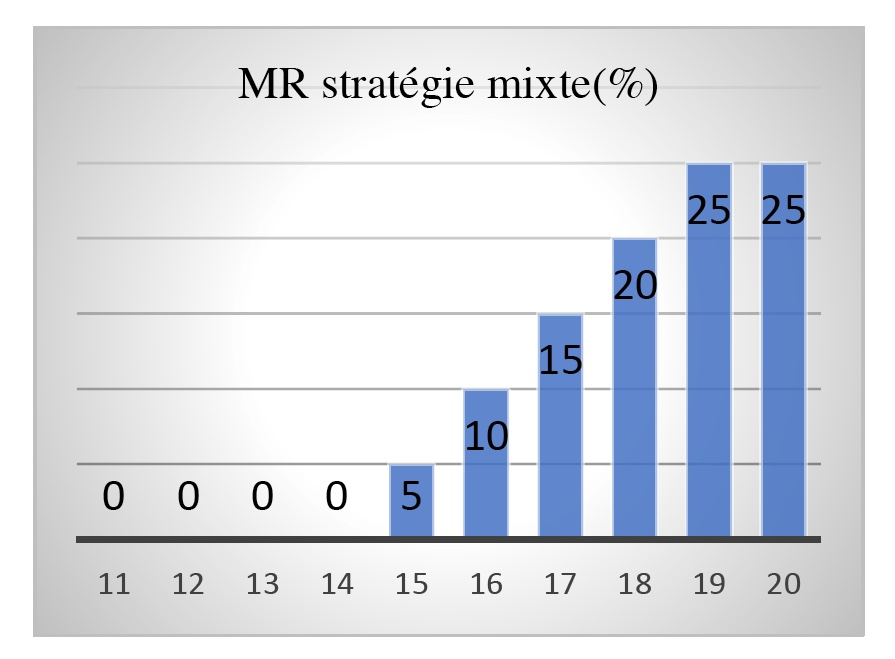
\includegraphics[height=5cm]{Articles-bons-a-composer/02_Umbhauer/02_Umbhauer_fr_Figures/02_Umbhauer_fr_figure-2.jpeg}
\end{figure}

\begin{figure}[h]
    \centering
    \caption{Équilibre de Nash symétrique en dans le jeu 11-20/bonus20 stratégies
mixtes dans le jeu 11-20/bonus20}
    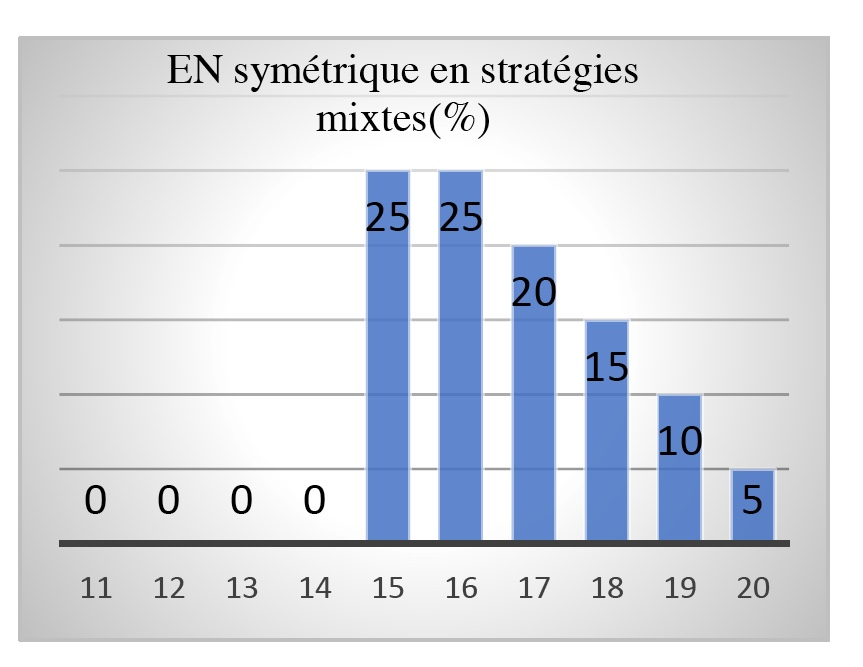
\includegraphics[height=5cm]{Articles-bons-a-composer/02_Umbhauer/02_Umbhauer_fr_Figures/02_Umbhauer_fr_figure-3.jpeg}
\end{figure}

% PROPOSITION 1

\begin{proposition}

a) Dans le jeu 11-T/bonus B, \(B \geq T > 11 + n\), n étant
l'entier naturel défini par \(\frac{n(n + 1)}{2} < B < \frac{(n + 1)(n + 2)}{2}\), la MR
stratégie mixte est donnée par~:

{\centering
$p_{i} = 0$, i de 11 à $T-n-1$, \\
$p_{T - n + i} = \frac{i + 1}{B}$, i de 0 à $n-1$,  \\
$p_{T} = 1 - \frac{n(n + 1)}{2B}$;\par}

b) Pour \(B \geq T > 11 + n\) et \(B=\frac{n(n + 1)}{2}\), les MR stratégies mixtes sont les combinaisons convexes des deux distributions suivantes :

{\centering
$p_{i} = 0$, i de 11 à $T-n-1$, \\
$p_{T - n + i} = \frac{i + 1}{B}$, i de 0 à $n-1$, \\
$p_{T} = 0$,\par}

et

{\centering
$p_{i} = 0$, i de 11 à $T-n$, \\
$p_{T - n + i} = \frac{i}{B}$, i de 1 à n;\par}

c) Le MR, z, est égal à
\(B + \frac{n(n + 1)(n + 2)}{6B}\ –\ (n + 1)\).
\end{proposition}

\begin{demonstration}
    Voir annexe~\ref{Annexe:Démonstration prop 1_Umbhauer}. \quad \blacksquare
\end{demonstration}

Le point \emph{a} est illustré dans le jeu d'Arad et Rubinstein avec \(T = B = 20\) et
\(n = 5\). Le point~\emph{b} est illustré pour \(B = T = 21\) et \(n = 6\). Deux distributions,

{\centering \(p_{i} = 0\) pour \emph{i} de 11 à 14,
$p_{15} = \frac{1}{21}, p_{16} = \frac{2}{21}, p_{17} = \frac{3}{21}, p_{18} = \frac{4}{21}$,\par}

{\centering \(p_{19} = \frac{5}{21}, p_{20} = \frac{6}{21}, p_{21} = 0\)\par}

\noindent et

{\centering $p_{i} = 0$ pour \emph{i} de 11 à 15,
$p_{16} = \frac{1}{21}, p_{17} = \frac{2}{21}, p_{18} = \frac{3}{21}, p_{19} = \frac{4}{21}$,\par} 

{\centering $p_{20} = \frac{5}{21}, p_{21} = \frac{6}{21}$,\par}

\noindent conduisent au regret minimal 50/3, et toute combinaison convexe des deux
distributions conduit également à ce regret minimal.

La proposition 1 donne lieu aux commentaires suivants.

Quand \(\frac{n(n + 1)}{2} < B,\) $p_T$
($p_20$ dans le jeu d'Arad et Rubinstein) est juste
le complément à 1 de la somme \(\sum_{i = T - n}^{T - 1}p_{i}\). Dans le
jeu d'Arad et Rubinstein, $p_T = p_{T-1} = 5/20$. Ainsi, par construction, la
probabilité de jouer le plus grand montant (qui correspond au
raisonnement de niveau-0) est inférieure ou égale à la probabilité de
jouer le montant \(T - 1\) (montant du raisonnement de niveau-1)

La proposition montre que, pour \(B > \frac{n(n + 1)}{2}\),
\emph{p\textsubscript{i}} est linéairement croissante en \emph{i}, pour
\emph{i} de \(T - n\) à \(T - 1\): $\ p_{T - n} = \frac{1}{B}$, $p_{T - 1} = \frac{n}{B}$ et $p_{i} - p_{i - 1} = 1/B$. Pour \(B = \frac{n(n + 1)}{2}\), $p_i$ est également croissante en \emph{i}, pour \emph{i} de \(T - n\) à \(T - 1\), mais $p_T$ peut être supérieure,
inférieure ou égale à $p_{T-1}$.

Ces probabilités croissantes sont en accord avec la conjecture émise en
amont : un joueur qui joue \emph{x} regrette toujours de ne pas avoir
joué \(y - 1\), \emph{y} étant le montant joué par l'adversaire, mais ce
regret décroît en \emph{x}, car \(y - 1 + B - x\) est décroissant en
\emph{x}.

La proposition 1 va au-delà du résultat de \textcite{garciapola2020}. Cet auteur a montré qu'une application itérée du MR en
stratégies pures et le raisonnement de niveau-1 conduisent à
sélectionner le même montant, 19, dans le jeu d'Arad et Rubinstein. La
proposition 1 montre que la MR stratégie mixte coïncide avec une
distribution issue d'un raisonnement de niveau-\emph{k}, du niveau-1 au
niveau-\emph{n}, à condition que chaque étape additionnelle de
raisonnement soit réalisée par un nombre plus petit d'individus. Ainsi,
dans le jeu 11-20/bonus20, les MR probabilités correspondent à la
distribution observée avec des joueurs de niveau-\emph{k}, si 25 \% des
joueurs mènent un raisonnement de niveau-1 (\emph{i.e.} jouent 19), 20~\% font
un raisonnement de niveau-2 (\emph{i.e.} jouent 18), 15~\% font un raisonnement
de niveau-3 (\emph{i.e.} jouent 17), 10~\% font un raisonnement de niveau-4
(\emph{i.e.} jouent 16) et 5~\% font un raisonnement de niveau-5 (\emph{i.e.} jouent
15). D'où, malgré que la logique du MR n'ait aucun lien avec le
raisonnement de niveau-\emph{k}, le MR conduit à un comportement
similaire dans le jeu de demande 11-\emph{T} avec bonus \emph{B}, du
moins si on suppose que le pourcentage de joueurs aptes à mener un
raisonnement de niveau-\emph{k} décroît avec \emph{k}. Comme
\emph{p\textsubscript{i} =} 0 pour \(i < T - n\), ce résultat, pour être
compatible avec le raisonnement de niveau-\emph{k}, exige que personne
ne soit capable de mener un raisonnement de profondeur supérieure ou
égale au niveau-\((n + 1)\). Toutefois, \(B \geq T > 11 + n\) et
\(B > n(n + 1)/2\) impliquent \(n \geq 5\), aussi cette limite de
profondeur de raisonnement n'est pas vraiment restrictive, car dans la
réalité les joueurs font rarement plus de quatre itérations (raisonnement de
niveau-4) (voir par exemple \textcite{crawford2013}). Plus précisément, même
s'ils sont aptes à faire plus d'itérations, ils hésitent souvent à en
faire davantage car ils craignent que les autres joueurs n'en soient pas
capables\footnote{C'est donc la théorie de l'esprit (\textit{theory of mind}),
  c'est-à-dire l'habileté à se glisser dans la façon de raisonner de
  l'autre, qui conduit souvent à stopper un raisonnement au plus tard au
  niveau-4.}.

Étant donné que \emph{n} est croissant en \emph{B}, la proposition 1
montre également que la profondeur de raisonnement des acteurs croît en
fonction du gain qu'ils peuvent obtenir, ce qui est conforme à un
résultat obtenu par \textcite{alaoui2016}. Ainsi par exemple, dans
le jeu de demande 11-20 avec un bonus \(B\) qui vaut 30 au lieu de 20,
la profondeur de raisonnement atteint 7, vu que la MR stratégie mixte
devient~: $p_{i} = 0$, $i$ de 11 à 12, $p_{13} = \frac{1}{30}$, $p_{14} = \frac{2}{30}$, $p_{15} = \frac{3}{30}$, $p_{16} = \frac{4}{30}$, $p_{17} = \frac{5}{30}$, $p_{18} = \frac{6}{30}$, $p_{19} = \frac{7}{30}$, $p_{20} = \frac{2}{30}$.


\section{MINIMAX REGRET, ÉQUILIBRE DE NASH ET GAIN ESPéRé}
\label{section:Minimax Reg équilibre}

En comparant les figures 2 et 3 on voit que les probabilités de la
figure 3, pour \emph{x} de 15 à 20, sont symétriques à celles de la
figure 2, par rapport à l'axe vertical \(x = 17,5\). On dira simplement
qu'elles sont <<inversées>>. Ce lien étonnant pousse à la réflexion car,
usuellement, il n'y a aucun lien évident entre les stratégies
sélectionnées par l'EN et le MR (voir par exemple \textcite{umbhauer2022}).
Dans les jeux 11-\emph{T}/bonus\emph{B}, il y a au contraire un lien
fort entre les deux concepts, précisé dans la proposition 2.

% PROPOSITION 2

\begin{proposition}
Dans les jeux 11-T/bonusB, avec \(B \geq T > 11 + n\), $n$ étant l'entier naturel vérifiant \(\frac{n(n + 1)}{2} < B < \frac{(n + 1)(n + 2)}{2}\), les actions
jouées à l'EN symétrique en stratégies mixtes sont les mêmes que celles
jouées dans la MR stratégie mixte. Mais les probabilités attribuées aux
montants joués sont inversées (elles sont symétriques par rapport à
l'axe vertical \(x = T - n/2\)), c'est-à-dire :
\(q_{i} = p_{2T - n - i}\) pour $i$ de \(T - n\) à $T$, où
$q_i$, respectivement $p_i$, est la
probabilité attribuée au montant $i$ par l'EN symétrique en stratégies
mixtes, respectivement la MR stratégie mixte.   
\end{proposition}

\begin{demonstration}
    Pour le montant joué $i$, le gain
\(i(1 - q_{i + 1}) + (i + B)q_{i + 1} = i + B{q\ }_{i + 1}\) doit être
égal au gain obtenu avec le montant $T$, à savoir $T$. Ainsi
\(q_{i} = \ (T - i + 1)/B\) pour $i$ de $T$ à \(T - n + 1\) et
\(q_{T - n} = 1 - \frac{n(n + 1)}{2B}\) , avec
\(\frac{n(n + 1)}{2} < B < \frac{(n + 1)(n + 2)}{2}\). Il en découle que
les montants $i$, pour \(i < T - n\), conduisent à un gain
inférieur, d'où \(q_{i} = 0\). \quad \blacksquare
\end{demonstration}

Par exemple, dans le jeu d'Arad et Rubinstein, les probabilités de l'EN
symétrique sont \(q_{i} = 0\) pour \emph{i} de 11 à
14, $q_{15} = \frac{5}{20}$, $q_{16} = \frac{5}{20}$, $q_{17} = \frac{4}{20}$, $q_{18} = \frac{3}{20}$, $q_{19} = \frac{2}{20}$ et $q_{20} = \frac{1}{20}$ (tableau~1 et figure~3).

Ainsi, alors que les MR probabilités croissent linéairement de
\(p_{T - n} = 1/B\) à \(p_{T - 1} = n/B\) (\emph{p\textsubscript{T}}
étant le complément à 1), les probabilités de l'EN symétrique
décroissent linéairement de\(\ q_{T - n + 1} = n/B\) à \(q_{T} = 1/B\ \)
($q_{T-n}$ étant le complément à 1).

\vspace{0.2cm}
Ce lien surprenant est dû à la structure des jeux étudiés. Nous
illustrons ce fait dans le jeu 11-20/bonus20. Les équations liées au MR
(1) qui sont vérifiées avec égalité sont rappelées ci-après (équations~(2)). On peut observer que ces équations sont les équations de l'EN en
stratégies mixtes, qui assurent que le joueur~2 obtienne le même gain
avec toutes ses stratégies pures dans le jeu à somme nulle de la matrice~3. Ainsi les probabilités $p_i$ du joueur~1 obtenues
par la logique du MR correspondent à la stratégie mixte du joueur~1 à
l'EN du jeu de la matrice~3.
%
\begin{align*}
19p_{15} + 18p_{16} + 17p_{17} + 16p_{18} + 15p_{19} + 14p_{20} &= z \\
0p_{15} + 19p_{16} + 18p_{17} + 17p_{18} + 16p_{19} + 15p_{20} &= z \\
21p_{15} + 0p_{16} + 19p_{17} + 18p_{18} + 17p_{19} + 16p_{20} &= z \\
22p_{15} + 21p_{16} + 0p_{17} + 19p_{18} + 18p_{19} + 17p_{20} &= z \\ \tag{2}
23p_{15} + 22p_{16} + 21p_{17} + 0p_{18} + 19p_{19} + 18p_{20} &= z \\
24p_{15} + 23p_{16} + 22p_{17} + 21p_{18} + 0p_{19} + 19p_{20} &= z \\
p_{15} + p_{16}{+ p}_{17} + p_{18} + p_{19} + p_{20} &= 1
\end{align*}

\begin{table}[h!]
\centering
Matrice 3\par
\vspace{0.2cm}
\label{matrice3}
\resizebox{.65\linewidth}{!}{
\begin{tabular}{lc | *{6}{c} |}
\multicolumn{8}{c}{P12} \tabularnewline
& \multicolumn{1}{l}{} & 15 & 16 & 17 & 18 & 19 & \multicolumn{1}{c}{20} \tabularnewline
\cline{3-8}
& 15 & (--19,19) & (0,0) & (--21,21) & (--22,22) & (--23,23) &
(--24,24) \tabularnewline
& 16 & (--18,18) & (--19,19) & (0,0) & (--21,21) & (--22,22) &
(--23,23) \tabularnewline
Pl1 & 17 & (--17,17) & (--18,18) & (--19,19) & (0,0) &
(--21,21) & (--22,22) \tabularnewline
& 18 & (--16,16) & (--17,17) & (--18,18) & (--19,19) & (0,0) &
(--21,21) \tabularnewline
& 19 & (--15,15) & (--16,16) & (--17,17) & (--18,18) & (--19,19)
& (0,0) \tabularnewline
& 20 & (--14,14) & (--15,15) & (--16,16) & (--17,17) & (--18,18)
& (--19,19) \tabularnewline
\cline{3-8}
\end{tabular}}
\end{table}

Les équations de Karush Kuhn Tucker (voir l'annexe\ref{Annexe:Démonstration prop 1_Umbhauer} dont elles sont
extraites) qui découlent du programme de minimisation deviennent les
équations~(3) (après avoir enlevé les multiplicateurs égaux à 0) :
%
\begin{align*}
19\lambda_{15} + 0\lambda_{16} + 21\lambda_{17} + 22\lambda_{18} + 23\lambda_{19} + 24\lambda_{20} + \lambda &= 0 \\
18\lambda_{15} + 19\lambda_{16} + 0\lambda_{17} + 21\lambda_{18} + 22\lambda_{19} + 23\lambda_{20} + \lambda &= 0 \\
17\lambda_{15} + 18\lambda_{16} + 19\lambda_{17} + 0\lambda_{18} + 21\lambda_{19} + 22\lambda_{20} + \lambda &= 0 \\ \tag{3}
16\lambda_{15} + 17\lambda_{16} + 18\lambda_{17} + 19\lambda_{18} + 0\lambda_{19} + 21\lambda_{20} + \lambda &= 0 \\
15\lambda_{15} + 16\lambda_{16} + 17\lambda_{17} + 18\lambda_{18} + 19\lambda_{19} + 0\lambda_{20} + \lambda &= 0 \\
14\lambda_{15} + 15\lambda_{16} + 16\lambda_{17} + 17\lambda_{18} + 18\lambda_{19} + 19\lambda_{20} + \lambda &= 0 \\
1 - \sum_{i = 15}^{20}{\lambda_{i}} &= 0
\end{align*}

Ces équations assurent que le joueur 1 réalise le même gain avec toutes
ses stratégies pures dans le jeu à somme nulle de la matrice 3. Aussi
les multiplicateurs KKT $\lambda_i$ deviennent la
stratégie mixte du joueur 2 à l'EN du jeu à somme nulle de la matrice~3.

Or il y a un lien fort entre le jeu à somme nulle de la matrice~3 et le
jeu réellement joué par les joueurs, dès lors qu'on écrit ce jeu à
l'envers, ce qui est fait dans la matrice~4.

\begin{table}[h!]
\centering
Matrice 4\par
\vspace{0.2cm}
\label{matrice4}
\resizebox{.65\linewidth}{!}{
\begin{tabular}{lc | *{6}{r} | }
\multicolumn{8}{c}{P12} \tabularnewline
& \multicolumn{1}{l}{} & 20 & 19 & 18 & 17 & 16 & \multicolumn{1}{c}{15} \tabularnewline
\cline{3-8}
& 20 & (20,20) & (20,39) & (20,18) & (20,17) & (20,16) & (20,15) \tabularnewline
& 19 & (39,20) & (19,19) & (19,38) & (19,17) & (19,16) & (19,15) \tabularnewline
Pl1 & 18 & (18,20) & (38,19) & (18,18) & (18,37) & (18,16) & (18,15) \tabularnewline
& 17 & (17,20) & (17,19) & (37,18) & (17,17) & (17,36) & (17,15) \tabularnewline
& 16 & (16,20) & (16,19) & (16,18) & (36,17) & (16,16) & (16,35) \tabularnewline
& 15 & (15,20) & (15,19) & (15,18) & (15,17) & (35,16) & (15,15) \tabularnewline
\cline{3-8}
\end{tabular}}
\end{table}

En effet, égaliser les gains du joueur 2 dans deux colonnes adjacentes
de la matrice 4 conduit exactement aux mêmes calculs qu'égaliser les
gains des mêmes colonnes de la matrice 3, car ces égalisations
exploitent les différences 1 et 19 qui sont présentes dans les deux
matrices exactement aux mêmes emplacements.

Par exemple, égaliser les gains du joueur 2 dans les deux premières
colonnes des deux matrices conduit aux équations~:
\begin{equation*}
\begin{split}
  20p_{20} + 20p_{19} + 20p_{18} + 20p_{17} + 20p_{16} + 20p_{15} = 39p_{20} + 19p_{19} + 19p_{18}\\ + 19p_{17} + 19p_{16} + 19p_{15}  
\end{split}
\end{equation*}

\noindent \text{pour la matrice 4 (on note \emph{p\textsubscript{i}} la probabilité du
joueur 1 de jouer \emph{i})} et
\begin{equation*}
\begin{split}
    19p_{15} + 18p_{16} + 17p_{17} + 16p_{18} + 15p_{19} + 14p_{20} = 0p_{15} + 19p_{16} + 18p_{17}\\ + 17p_{18} + 16p_{19} + 15p_{20}
\end{split}
\end{equation*}

\noindent \text{pour la matrice 3.}

Ces équations conduisent à \(p_{20} = \frac{1}{20}\) pour la matrice 4
et \(p_{15} = \frac{1}{20}\) pour la matrice 3. Et c'est ainsi qu'on
obtient les probabilités inversées.

Ajoutons quelques remarques au sujet des gains.

On peut commencer par observer que le MR, si les deux joueurs jouent
leur MR stratégie mixte, conduit au gain espéré 21.5 dans le jeu d'Arad
et Rubinstein, soit un gain plus élevé que le gain espéré 20 de l'EN
symétrique.

Ce résultat se généralise à tout jeu \(11 - T/bonusB\), où
\(B \geq T > n + 11\), \emph{n} étant défini par
\(\frac{n(n + 1)}{2} < B < \frac{(n + 1)(n + 2)}{2}\) (partie \emph{a}
de la proposition 3).

Toutefois minimiser les regrets n'est adapté que dans un contexte à
forte incertitude stratégique où l'adversaire est susceptible de jouer
n'importe quelle stratégie. Aussi un joueur jouant la MR stratégie mixte
n'est pas nécessairement confronté à un adversaire jouant également
cette stratégie. Il est donc plus pertinent de calculer le gain obtenu
par un joueur jouant la MR stratégie mixte face à tout montant
potentiellement joué par son adversaire. Ce calcul donne lieu à la
partie (\emph{b}) de la proposition 3.

% PROPOSITION 3

\begin{proposition}

a) Dans tout jeu 11-T/bonusB, avec \(B \geq T > n + 11\), n
étant l'entier naturel vérifiant \(\frac{n(n + 1)}{2} < B < \frac{(n + 1)(n + 2)}{2}\), le gain espéré avec le MR, lorsque les deux joueurs jouent leur MR stratégie
mixte, vaut \(T + n - \frac{n(n + 1)(n + 2)}{3B}\). Ce gain est
entre \(T + \frac{n - 4}{3}\) et \(T + \frac{n}{3}\), et
est donc strictement plus grand que T, vu que n est plus grand que 4. Il
est donc plus grand que le gain espéré de l'EN symétrique, qui, par
construction, est toujours égal à T, quel que soit n. \par
b) On suppose maintenant que l'adversaire joue le montant~y. Alors un joueur qui joue la MR stratégie mixte obtient un paiement moyen égal à~:

{\centering
\(y - 1 + B - z = y + n - \frac{n(n + 1)(n + 2)}{6B}\) si \(y \geq \ T - n\),\\
\(T - \frac{n(n + 1)(n + 2)}{6B}\) si \(y < T - n\).\par}

Ainsi le gain le plus bas auquel mène la MR stratégie mixte est
entre \(T - (n + 2)/3\) et \(T - n/3\) et le gain le plus
élevé est \(T + n - \frac{n(n + 1)(n + 2)}{6B}\), qui est entre
\(T + 2(n - 1)/3\) et \(T + 2n/3\ \). La MR stratégie mixte
conduit à un gain supérieur à celui de l'EN symétrique dès que
\(y > T - n + \frac{n(n + 1)(n + 2)}{6B}\), \(T - n + \frac{n(n + 1)(n + 2)}{6B}\)
étant entre \(T - 2n/3\) et \(T - 2(n - 1)/3\).    
\end{proposition}

\begin{demonstration}
    Voir l'annexe~\ref{Annexe:Démonstration prop 3_Umbhauer}. \quad \blacksquare
\end{demonstration}

Par exemple (partie \emph{a}), pour \(T = 100,\ B = 100,\ n = 13\), le
paiement espéré quand les deux joueurs jouent la MR stratégie mixte est
103,9 au lieu de 100 (paiement espéré dans l'EN symétrique). Toutefois,
si on reste dans l'esprit du jeu d'Arad et Rubinstein et qu'on garde
\(B = T\), alors la différence entre les gains associés à l'EN et à la
MR stratégie mixte, comparée à \emph{T}, reste faible. En effet, comme
\(n(n + 1)/2 < B\), on a \(n/3 < \sqrt{2B}/3\) et, vu que le gain espéré
avec le MR est plus faible que \(T + n/3\), il est plus faible que
\(T + \sqrt{2T}/3\). Aussi la différence entre les deux gains est certes
croissante en \emph{T}, mais la différence relative par rapport à
\emph{T}, \(\frac{\sqrt{2T}}{3T},\) est décroissante en \emph{T}. Ce
résultat change quand \emph{B} peut être nettement plus grand que
\emph{T} (avec \(T > 11 + n\)). Dans ce cas, le gain additionnel peut
avoisiner \((T - 11)/3\), un montant qui peut être conséquent.

La partie~\emph{b} peut être illustrée dans le jeu d'Arad et Rubinstein
(tableau 2).

\begin{table}[h!]
\caption{Gain moyen de la MR stratégie mixte dans le jeu
  11-20/bonus20 en fonction du montant choisi par l'adversaire}\label{tabl2}
\centering
\resizebox{\linewidth}{!}{
\begin{tabular}{l*{10}{D{6mm}}}
\toprule
Montant demandé \par par l'adversaire & \centering 11 & \centering 12 & \centering 13 & \centering 14 & \centering 15 & \centering 16 & \centering 17 & \centering 18 & \centering 19 & \centering 20 \tabularnewline
\midrule
MR paiement & 18,25 & 18,25 & 18,25 & 18,25 & 18,25 & 19,25 & 20,25 &
21,25 & 22,25 & 23,25 \tabularnewline
\bottomrule
\end{tabular}}
\end{table}

Ainsi, même si l'adversaire joue les nombres -- peu fréquemment joués~--
de 11 à 15, le gain du joueur est plutôt grand, et le fait que ce gain
soit plus faible que le gain 20 de l'EN en stratégies mixtes doit être
contrebalancé par le fait qu'il est plus grand que 20 lorsque
l'adversaire joue les nombres -- plus fréquemment joués~-- de 17 à 20.

Si \(T = B = 100\), \(n = 13\)\emph{,} le tableau de gains devient le
tableau 3:

\begin{table}[h!]
\caption{Gain moyen de la MR stratégie mixte dans le jeu
  11-100/bonus100 en fonction du montant choisi par l'adversaire}\label{tabl3}
\centering
\resizebox{\linewidth}{!}{
\begin{tabular}{l*{14}{D{6mm}}}
\toprule
 Montant demandé par l'adversaire & Toute valeur $\leq$~87 & 88 & 89 & 90 & 91 & 92 & 93 & 94 & 95 & 96 & 97 & 98 & 99 & 100 \tabularnewline
\midrule
MR paiement & 95,45 & 96,45 & 97,45 & 98,45 & 99,45 & 100,45 & 101,45 &
102,45 & 103,45 & 104,45 & 105,45 & 106,45 & 107,45 & 108,45 \tabularnewline
\bottomrule
\end{tabular}}
\end{table}

À nouveau les paiements sont plutôt attractifs. Ils sont plus faibles
que le gain 100 de l'EN symétrique quand l'adversaire joue des nombres
inférieurs à 92 (mais restent élevés, 95,45 au moins au lieu de 100)
mais ils sont plus grands que 100 (et croissent jusqu'à 108,45) quand
l'adversaire jouent des nombres supérieurs ou égaux à 92.

Plus généralement, quand \emph{n} devient grand, alors le paiement
minimal auquel peut conduire le MR, proche de \(T - n/3\), peut certes
devenir faible en comparaison du paiement \emph{T} de l'EN (surtout si
\emph{B} est beaucoup plus grand que \emph{T}). Mais, dans le même
temps, le montant minimal \emph{y} de l'adversaire, autour de
\(T - 2n/3\), à partir duquel le MR conduit à un gain plus élevé que le
gain de l'EN, devient beaucoup plus petit. Aussi, à condition que
l'adversaire joue des nombres plutôt élevés (ce qui est usuellement
observé dans les expériences), la MR stratégie mixte conduit à des gains
plus élevés que l'EN.

\section{COMMENTAIRES SUR LES MINIMAX REGRETS, \\ VARIANTES DU JEU DE DEMANDE 11-20 \\ AVEC BONUS 20 ET AVERSION AU RISQUE}
\label{section:Commentaires sur MR}

\textcite{arad2012} ont observé que dans leur jeu
11-20/bonus20, seul un petit nombre de leurs étudiants, moins de 20~\%,
faisaient plus de trois itérations, et ce malgré qu'une itération
supplémentaire --~à savoir passer du montant \emph{x} de niveau-\emph{k}
au montant $x-1$ de niveau-\emph{k}+1~-- ne requiert que très peu
de compétences cognitives. Aussi ils ont essayé de stimuler davantage
d'itérations en renforçant la légitimité du montant 20 comme point
d'ancrage des itérations.

Pour ce faire ils ont introduit une version cyclique, qui ne diffère de
la version de base que par le fait qu'un joueur qui joue 20 obtient le
bonus 20 si son adversaire joue 11. Le choix de 20 est ainsi encore plus
attractif que dans la version initiale du jeu~: 20 devient donc encore
plus spontanément la stratégie naturelle de niveau-0. En ce qui concerne
les étudiants de Strasbourg, il est probable que ce changement aurait
poussé certains des étudiants jouant 13, 14 et 15 dans la version
initiale du jeu d'Arad et Rubinstein à choisir 18, 19 et 20. En effet la
moitié de ces étudiants justifiaient le jeu de 13, 14 et 15 par un
raisonnement de niveau-\emph{k} débutant par 15 ou 16 (donc fixaient 15
ou 16 comme l'action de niveau-0). Toutefois, renforcer 20 en tant que
point d'ancrage du raisonnement de niveau-\emph{k} n'a pas augmenté la
profondeur de raisonnement\footnote{Cela est peut-être dû au fait que
  faire plus d'itérations ne conduit pas à un gain additionnel ; dans
  les faits, le paiement additionnel de 20 dans cette version cyclique
  n'est obtenu qu'en jouant 20 lorsque l'adversaire joue 11, ce qui
  nécessite 10 itérations, un nombre généralement non atteint (plus
  exactement, un joueur doit espérer que l'adversaire joue 11, donc mène
  un raisonnement de niveau-9, ce qu'il ne fait généralement pas).}. Au
contraire, la version cyclique a augmenté le nombre de joueurs de
niveau-1, comme on peut le voir dans le tableau~4. L'EN symétrique reste
lui inchangé ainsi que le paiement espéré 20 à cet équilibre.

Étudions comment évolue la MR stratégie mixte dans cette nouvelle
version du jeu.

En fait, pour établir la MR stratégie mixte dans ce nouveau jeu, il
suffit de changer la première contrainte dans (1). Cette contrainte
devient~:
\[29p_{11} + 28p_{12} + 27p_{13} + 26p_{14} + 25p_{15} + 24p_{16} + 23p_{17} + 22p_{18} + 21p_{19} + 0p_{20} \leq z.\]
Si on associe cette contrainte à la dernière, on obtient la relation
additionnelle \(1 + 20p_{19} = 20p_{20}\), ce qui explique une
distribution de probabilités strictement croissante de 15 à 20. Il
s'ensuit que les probabilités dans la version cyclique sont pratiquement
les mêmes que dans la version initiale du jeu, excepté qu'elles sont un
peu plus faibles pour les montants de 15 à 19, et que la probabilité
attribuée à 20 est plus élevée (29,17~\% au lieu de 25~\%). Cette
distribution, même si on se limite aux nombres de 16 à 20, est
différente de la distribution obtenue par AR dans ce nouveau jeu (la
valeur \emph{p} du test du khi-deux vaut 0,015), mais les deux
distributions partagent un point commun important : elles sont
strictement croissantes de 15 à 19\footnote{De façon assez surprenante,
  la distribution d'AR (72~joueurs) dans la version cyclique, lorsqu'on
  se limite aux montants de 16 à 20, n'est pas significativement
  différente de la distribution de Strasbourg pour la version initiale
  -non cyclique- du jeu (test du khi-deux, \(p = 0,15\)). En quelque
  sorte, cela peut signifier que les étudiants de Strasbourg ont
  spontanément fait de 20 un point d'ancrage important.}. De plus, la MR
stratégie mixte conduit à des gains élevés, peu importe le montant
choisi par l'adversaire (voir tableau 4).

\begin{table}[h!]
\caption{Distribution expérimentale d'AR, minimax regret en
  stratégies mixtes, équilibre de Nash symétrique et paiement moyen du
  minimax regret dans la version cyclique d'AR}\label{tabl4}
\centering
\resizebox{\linewidth}{!}{
\begin{tabular}{l*{10}{D{6mm}}}
\toprule
Montant demandé dans la version cylique & \centering 11 & \centering 12 & \centering 13 & \centering 14 & \centering 15 & \centering 16 & \centering 17 & \centering 18 & \centering 19 & \centering 20 \tabularnewline
\midrule
Expérience d'AR (\%) & 1 & 1 & 0 & 1 & 0 & 4 & 10 & 22 & 47 & 13 \tabularnewline
MR strategie (\%) & 0 & 0 & 0 & 0 & 4,17 & 9,17 & 14,17 & 19,17 & 24,17 &
29,17 \tabularnewline
EN symétrique (\%) & 0 & 0 & 0 & 0 & 25 & 25 & 20 & 15 & 10 & 5 \tabularnewline
MR paiement en fonction du montant demandé par l'adversaire & 24,21 & 18,375 &
18,375 & 18,375 & 18,375 & 19,21 & 20,21 & 21,21 & 22,21 & 23,21 \tabularnewline
\bottomrule
\end{tabular}}
\end{table}

Plus généralement, dans toutes les variantes de leur jeu 11-20/bonus20
étudiées dans AR [2012], Arad et Rubinstein ont rarement observé des
étudiants effectuant plus de trois itérations. Étant donné le peu de
ressources cognitives nécessaires pour réaliser plus de 3 itérations
dans ces jeux, ils en ont déduit qu'il devait exister un seuil
d'itérations \emph{k} supérieur, que les acteurs ne franchissent pas ou
ne souhaitent pas franchir. Nous arguons toutefois dans cet article que
le raisonnement de niveau-\emph{k} n'est pas seul à l'œuvre dans les
jeux étudiés : il doit au moins partiellement être contrebalancé par la
façon dont les individus gèrent les regrets, le regret de ne pas obtenir
le bonus et le regret de ne pas avoir le gain certain 20. Un simple
regard aux explications apportées par les étudiants dans l'expérience en
classe de Strasbourg montre qu'ils parlent de regrets. Par exemple,
lorsqu'ils jouent 19, ils disent qu'« au plus ils regrettent l'unité
additionnelle qu'il auraient pu avoir en jouant 20, mais qu'en échange
ils ont l'opportunité de gagner 39 si l'adversaire joue 20\footnote{Le
  fait qui importe dans cette phrase est qu'elle ne contient pas le
  terme~distribution de probabilités. Le jeu de 19 ne s'explique pas par
  le fait que 19 est la meilleure réponse (comportement de niveau-1)
  dans un environnement perturbé où les joueurs de niveau-0 joueraient
  20 avec une forte probabilité mais inférieure à 1 (ce qui conduirait à
  comparer les stratégies 19 et 20, et donc des différences de $-1$ et
  20). Le comportement exprimé dans cette phrase est en accord avec le
  MR car le joueur joue 19 quelle que soit la demande (ou distribution
  de probabilités sur les demandes) de l'adversaire. Il joue 19 car au
  plus il regrette 1 en comparaison avec le gain certain 20 (il ne
  regrette donc pas un manque de prudence) et il ne regrette pas le
  potentiel bonus 20 (vu qu'il garde l'opportunité de l'obtenir).}~». De
même, quand ils jouent 16, 17, 18 ils ajoutent souvent au raisonnement
de niveau-\emph{k} (quand ils le font) l'observation qu'au plus ils perdent 4,
3 ou 2 par comparaison au jeu de 20. Ainsi ils ne calculent pas les
regrets en comparant les paiements des meilleures réponses aux paiements
obtenus, mais en comparant le gain sûr \emph{x} qu'ils obtiennent en
jouant \emph{x}, avec le gain sûr de 20 qu'ils pourraient obtenir en
jouant 20. Or le regret quand l'adversaire joue \emph{y}
\(( \neq x + 1)\), tel qu'il est défini par le concept de MR, est
\(B + y - 1 - x\), et peut donc s'écrire \((20 - x) + B + y - 1 - 20\).
Aussi comparer le regret associé à deux stratégies \emph{x} et $x'$
quand l'adversaire joue \emph{y} (\(y \neq x + 1\) et
\(y \neq \ x’ + 1\)), revient à comparer \(20 - x\) et \(20 - x'\), les
montants que les étudiants prennent en compte quand ils parlent de
regrets. En fait, dans l'expérience en classe de Strasbourg, si peu
d'étudiants vont au-delà de trois itérations, ce qui les conduirait à jouer
un nombre \emph{x} inférieur à 17, cela tient au fait que ces regrets
deviennent larges quand \emph{x} est loin de 20.

Deux expériences qui montrent que le MR et le raisonnement de
niveau-\emph{k} sont tous deux présents dans le jeu 11-20/bonus20 sont
celles proposées par \textcite{goeree2018} (GLZ par la suite), qui
sont deux variantes du jeu d'Arad et Rubinstein. Dans ces variantes, GLZ
ont changé l'ordre des entiers naturels joués comme suit~: les joueurs
sont face à 10 boîtes alignées, numérotées de 11 à 20 dans le désordre.
Chaque joueur sélectionne une boîte et obtient le montant qui correspond
au numéro de la boîte. Et il obtient un bonus de 20 si la boîte qu'il
choisit est adjacente et à gauche de la boîte choisie par l'autre
joueur.

GLZ ont proposé les deux alignements de boîtes suivants (tableau 5):

\begin{table}[h!]
\caption{Les deux alignements proposés par Goeree, Louis et Zang [2018]}
\label{tab5}
\centering
\resizebox{\linewidth}{!}{
\begin{tabular}{l*{20}{c}}
\toprule
1\textsuperscript{er} alignement & & \cellcolor{gray!50}14 & & \cellcolor{gray!50}13 & & \cellcolor{gray!50}12 & & \cellcolor{gray!50}11 & & \cellcolor{gray!50}19 & & \cellcolor{gray!50}18 & & \cellcolor{gray!50}17 & & \cellcolor{gray!50}16 & & \cellcolor{gray!50}15 & & \cellcolor{gray!50}20 \tabularnewline
\midrule
% & & & & & & & & & & & & & & & & & & & & \tabularnewline
\midrule
2\textsuperscript{e} alignement & & \cellcolor{gray!50}19 & & \cellcolor{gray!50}18 & & \cellcolor{gray!50}17 & & \cellcolor{gray!50}16 & & \cellcolor{gray!50}15 & &
\cellcolor{gray!50}14 & & \cellcolor{gray!50}13 & & \cellcolor{gray!50}12 & & \cellcolor{gray!50}11 & & \cellcolor{gray!50}20 \tabularnewline % attention, l'espace entre la couleur et le chiffre est prise en compte, ce qui décale le nombre dans la boîte grise. C'est un bug, en attendant il faut "coller" la commande au nombre.
\bottomrule
\end{tabular}}
\end{table}

Ces deux alignements ont en commun le fait que seul le choix de (la
boîte) 20 ne peut jamais conduire au bonus et que le choix de toute
autre boîte fait obtenir le bonus dans un seul cas. Ainsi, dans le
1\textsuperscript{er} alignement, choisir (la boîte)15 conduit au bonus
quand l'adversaire choisit (la boîte) 20, 16 conduit au bonus quand
l'adversaire joue 15 et ainsi de suite. Le choix de 20, puisqu'il
correspond à la boîte la plus à droite et qu'il conduit au plus grand
gain certain sans aucun raisonnement est à nouveau la stratégie
naturelle de niveau-0 dans les deux alignements. Ainsi l'esprit du jeu
d'Arad et Rubinstein est respecté dans les deux jeux. Mais les
distributions expérimentales de GLZ obtenues pour les deux alignements
ne ressemblent pas à celles obtenues pour le jeu 11-20/bonus20. Elles
sont données en figure 4a et figure 4b.

\begin{figure}[h]
  \centering
  \caption{Distribution expérimentale de GLZ}
  \subfloat[Avec le 1\textsuperscript{er} alignement de boîtes]{%
    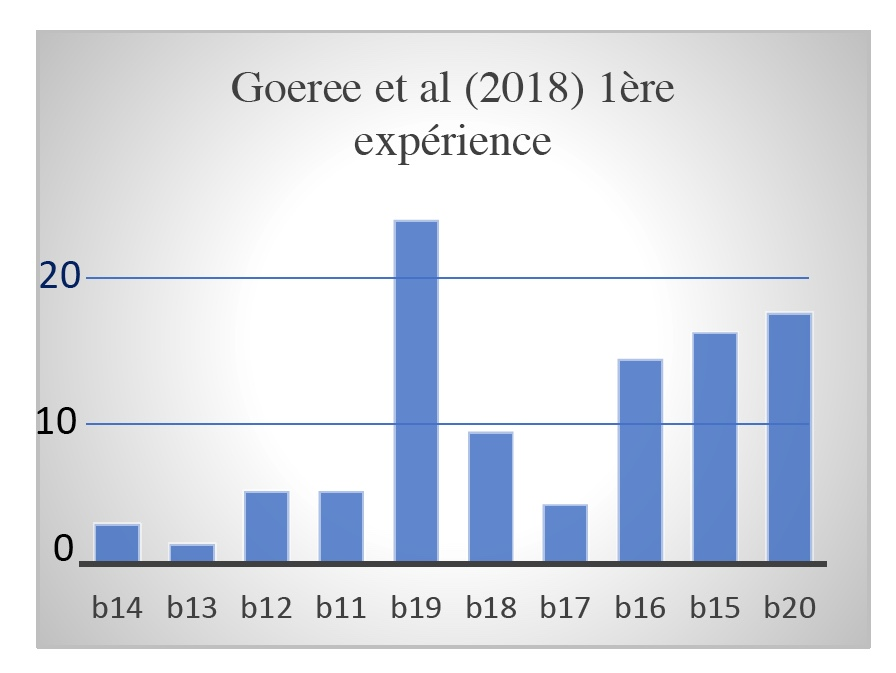
\includegraphics[height=5cm]{Articles-bons-a-composer/02_Umbhauer/02_Umbhauer_fr_Figures/02_Umbhauer_fr_figure-4a.jpeg}
    \label{fig:subfig1}%
  }
  \quad
  \subfloat[Avec le 2\textsuperscript{e} alignement de boîtes]{%
    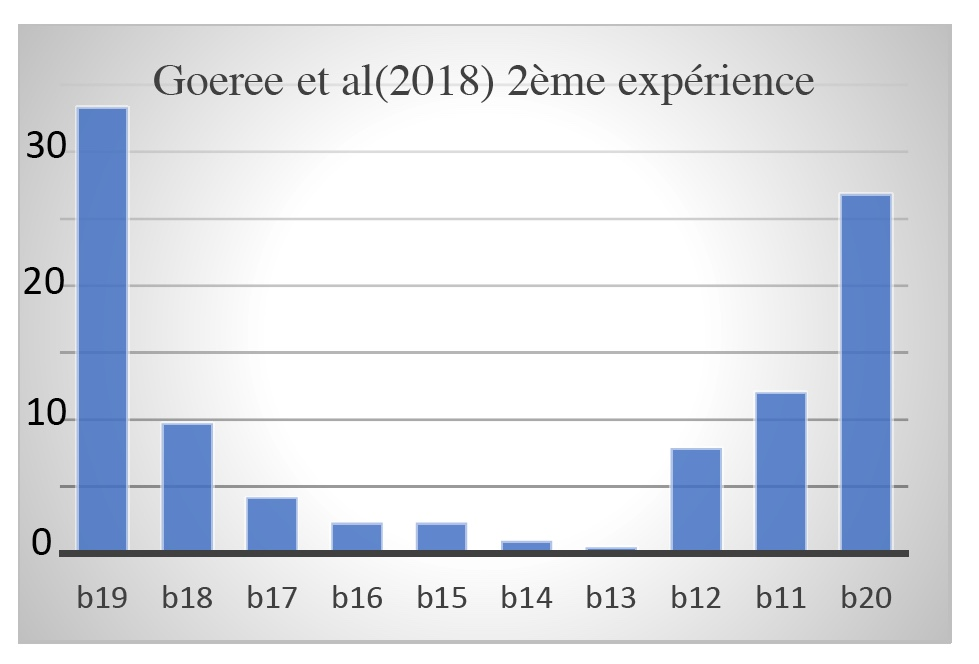
\includegraphics[height=5cm]{Articles-bons-a-composer/02_Umbhauer/02_Umbhauer_fr_Figures/02_Umbhauer_fr_figure-4b.jpeg}
    \label{fig:subfig2}%
  }
    \label{fig:mainfig}
\end{figure}

Dans les deux expériences il y a des joueurs qui ont un comportement
compatible avec un raisonnement de niveau-0, de niveau-1 et de niveau-2.
Dans la première expérience, les pourcentages de joueurs choisissant les
nombres 20, 15 et 16 sont plus grands que les pourcentages de joueurs
optant pour tout autre nombre, excepté 19. Dans la deuxième expérience,
les pourcentages associés aux nombres 20, 11 et 12 sont plus grands que
ceux associés aux autres nombres, excepté 19 et 18. Mais parallèlement,
tout d'abord, il y a très peu de joueurs de niveau-3 dans les deux
expériences et la somme des pourcentages de joueurs de niveaux 1, 2 et 3
est plutôt basse. Elle est inférieure à 35~\% dans la
1\iere{}~expérience, et plus faible que 21~\% dans la
2\ieme{}~expérience, d'où ces pourcentages sont très
différents de ceux obtenus pour le jeu 11-20/bonus20 (74~\% dans AR, 83~\%
dans LR, 60,4~\% dans l'expérience en classe de Strasbourg). Ensuite, 19
est le montant le plus souvent joué quel que soit son rang dans le
raisonnement de niveau-\emph{k} (19 est le montant de niveau-5 dans la
1\iere{}~expérience et le montant de niveau-9 dans la
2\ieme{}~expérience). Et même 18 est souvent joué dans les
deux expériences quel que soit son rang dans le raisonnement de
niveau-\emph{k}. Enfin, 20 est bien plus souvent joué que dans le jeu
11-20/bonus20 dans les deux expériences et plus particulièrement la
deuxième (27~\%). Ainsi, clairement, le fait que les grands nombres
conduisent à des gains certains élevés, et le fait que 19 assure le
2\ieme{} meilleur gain plus une opportunité d'obtenir le
bonus, jouent un rôle essentiel.

GLZ ont montré comment la connaissance commune d'un bruit dans le
comportement pouvait conduire à un comportement plus proche des données
expérimentales. Le MR permet aussi ce rapprochement. Il est intéressant
d'observer que la MR stratégie mixte est parfaitement insensible à
l'ordre des boîtes (à condition que 20 soit la boîte la plus à droite) :
ainsi le MR conduit à la même stratégie dans les deux jeux de GLZ et
dans le jeu 11-20/bonus20. Cela tient au fait que la structure des
regrets est la même dans les trois jeux. Par exemple, le fait que 19
conduise au gain 39 quand l'adversaire joue 18 (dans les deux
expériences de GLZ) conduit à une colonne de regrets qui est la même que
celle obtenue quand l'adversaire joue 20 dans le jeu d'Arad et
Rubinstein. Le fait que 15 mène à un gain de 35 quand l'adversaire joue
19 (1\iere{}~expérience) et 14 (2\ieme{}~expérience) conduit à une colonne de regrets qui est la même que celle
obtenue quand l'adversaire joue 16 dans le jeu d'Arad et Rubinstein. Et
ainsi de suite. Aussi minimiser les regrets conduit aux mêmes
contraintes dans les trois jeux (seul l'ordre des contraintes change).
Il découle que le MR conduit à la distribution de probabilités de la
figure 2. Certes, dans les jeux de GLZ, la MR stratégie mixte ne
ressemble plus à la distribution obtenue avec des joueurs de
niveau-\emph{k} (quand le pourcentage de joueurs de niveau-\emph{k}
décroît avec \emph{k}). Mais le MR est en accord avec les deux résultats
essentiels obtenus dans les expériences de GLZ. Premièrement, le MR
assigne la probabilité 0,25 à 19, une probabilité comparable aux
pourcentages obtenus dans les expériences de GLZ (24~\% dans la première
expérience, 33~\% dans la seconde expérience). Deuxièmement, la somme des
probabilités assignées à 18, 19 et 20 par le MR est 0,7, un nombre qui
est du même ordre que la somme des pourcentages de jeu de 18, 19 et 20
dans les expériences de GLZ (51~\% dans la première expérience, 70~\% dans
la seconde).

Ajoutons quelques mots au sujet de l'EN et de l'aversion au risque. Le
MR exploite le côté prudent des montants élevés (notamment 19) et le
regret associé à la non-obtention du bonus. \textcite{li2018}
exploitent également le côté prudent de 19 et 20 ; ils travaillent avec
l'EN et montrent que l'EN peut également être proche d'une distribution
expérimentale, à condition de prendre en compte l'aversion au risque.
Ils montrent notamment que la fonction d'utilité concave
\(1 - e^{- 0,15x}\), où \emph{x} est le montant choisi, conduit à un EN
qui correspond mieux à leurs données expérimentales, car cet équilibre
augmente notamment les probabilités attribuées à 18, 19 et 20. C'est
exact, mais cela ne veut pas dire que l'EN en stratégies mixtes est bien
adapté pour expliquer le comportement des joueurs. Ainsi il importe
d'observer que la fonction d'utilité \(1 - e^{- ax}\), avec \(a > 0\),
donne lieu à un EN qui se comporte comme l'EN usuel (neutre au risque) :
quand les montants joués à l'équilibre vont de \emph{x} à 20, la
probabilité attribuée à chaque nombre de \(x + 1\) à 20 décroît en ce
nombre, la probabilité de jouer \emph{x} étant le complément à 1. D'un
point de vue comportemental, il est plutôt étrange de voir \(x + 1\ \)
joué avec la plus forte probabilité alors que \(x - 1\ \)est joué avec
la probabilité~0. En fait, par définition, dans un EN en stratégies
mixtes, les probabilités d'un joueur ont pour unique fonction de
stabiliser (optimiser) le comportement des autres joueurs. Ainsi, dans
le jeu d'Arad et Rubinstein, elles ont pour seul rôle d'assurer le gain
20 à l'adversaire quel que soit le montant qu'il joue avec une
probabilité positive : cela n'est usuellement pas l'objectif des joueurs
dans les expériences.

\section{CONCLUSION}
\label{section:Conclusion Umbhauer_fr}

Le jeu 11-20/bonus20 d'Arad et Rubinstein est un jeu fort riche qui
suscite un comportement plus nuancé que le raisonnement de
niveau-\emph{k}.

Certes, les raisonnements de niveau-\emph{k}, et plus spécifiquement de
niveau-1, niveau-2 et niveau-3, sont observés dans les expériences. Dans
l'expérience en classe menée à Strasbourg, le raisonnement de
niveau-\emph{k} prédomine clairement chez les nombreux étudiants
(32,4~\%) qui jouent 17 et 18. La plupart des étudiants jouant 18 font
exclusivement un raisonnement de niveau-2, et 60~\% des étudiants jouant
17 font exclusivement un raisonnement de niveau-3. Près de la moitié des
5,8~\% d'étudiants jouant 16 font même un raisonnement de niveau-4.

Mais la minimisation des regrets joue également un rôle important. Nous
insistons ici sur une différence notable entre le jeu 11-20/bonus20
et le jeu de devinette, qui est le jeu le plus utilisé pour étudier le
raisonnement de niveau-\emph{k}. Dans un jeu de devinette, pour être le
gagnant (pour gagner 1), un joueur doit faire une itération
additionnelle par rapport aux autres joueurs, faute de quoi il gagne 0,
le gain des perdants. Ce n'est clairement pas le cas dans le jeu
d'Arad et Rubinstein où un joueur peut gagner une somme importante sans
faire la moindre anticipation. Jouer 20 conduit au gain élevé et certain
20, quel que soit l'adversaire rencontré. Dans l'expérience en classe,
le calcul du paiement moyen de chaque stratégie confrontée à toutes les
autres stratégies jouées montre que 20 procure le 4\ieme
meilleur gain (voir la figure~5). Et 19, le montant de niveau-1, conduit
au 2\ieme{} meilleur gain. Cela explique amplement
pourquoi les étudiants à Strasbourg qui jouent 19 et 20 généralement ne
justifient pas leur comportement par un raisonnement de niveau-\emph{k}.
Comme dit précédemment, la principale justification du jeu de 19 est en
accord avec le MR~: «~En jouant 19, je gagne 19 de manière certaine, ce
qui n'est pas loin de 20, et je garde l'opportunité de gagner 39 en
rencontrant un étudiant qui joue 20~».

\begin{figure}[h]
    \centering
    \caption{Paiement moyen associé à chaque montant demandé}
    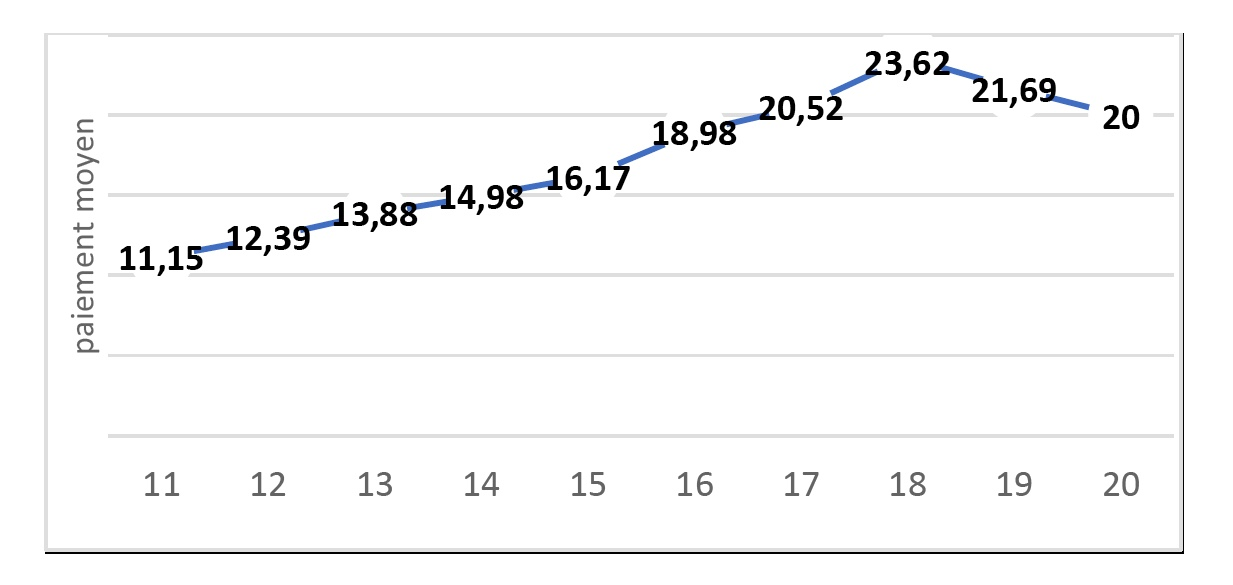
\includegraphics[height=5cm]{Articles-bons-a-composer/02_Umbhauer/02_Umbhauer_fr_Figures/02_Umbhauer_fr_figure-5.jpeg}
\end{figure}

Pour clore l'article, on peut mettre en lumière certaines particularités
de l'expérience en classe de Strasbourg, potentiellement liées au fait
que les étudiants disposaient de la matrice de la forme normale du jeu.
Cette matrice les a aidés à comparer leur gain avec celui de
l'adversaire dans chacune des configurations possibles et cela peut
expliquer certains comportements qui n'ont pas de lien, ni avec le
raisonnement de niveau-\emph{k}, ni avec la minimisation des regrets.

Ainsi beaucoup d'étudiants à Strasbourg, 8,3~\% d'entre eux, ont joué 11,
uniquement pour ne pas offrir à l'adversaire l'opportunité d'obtenir le
bonus. Il est bien connu que la peur de ne pas recevoir quelque chose
(ici le bonus) suscite l'envie que les autres ne l'obtiennent pas non
plus. Et jouer 11 est l'unique moyen d'empêcher l'adversaire d'obtenir
le bonus. En jouant 11, certains étudiants ont aussi cherché à minimiser
la différence potentielle de gains (à leur désavantage) entre les deux
joueurs. En effet, quand on joue 11, l'adversaire peut au plus gagner 9~unités de plus, alors qu'il peut gagner 19~unités supplémentaires si on
joue un montant différent de 11.

De façon moins extrême (et radicalement opposée), les étudiants qui ont
joué 19, respectivement 20, ont parfois justifié leur jeu en faisant
observer qu'ils gagnent plus que leur adversaire dans toutes les
situations, excepté une (quand l'adversaire joue 18, respectivement 19).
En effet, un étudiant qui joue 19 gagne plus que son adversaire si ce
dernier joue 20 ou un montant de 11 à 17 ; il ne gagne moins que lui que
si ce dernier joue 18. Ainsi il a un meilleur gain que son adversaire
dans 8 parmi les 10 configurations possibles. Il en va de même pour un
étudiant qui joue 20. Et on peut observer, de 18 à 11, que plus le
montant joué par un joueur est bas, moins les
configurations dans lesquelles il gagne plus que son adversaire sont nombreuses : en
jouant 18, il a un meilleur gain dans sept configurations, en jouant 11, il
n'a un meilleur gain que dans une configuration. Le fait que beaucoup
d'étudiants accordent plus d'importance à la différence de gains qu'au
gain obtenu est sûrement lié à leur vie de tous les jours. Beaucoup
d'entre eux~passent des concours où le seul objectif de chaque
participant est d'obtenir de meilleurs résultats que les autres
participants.

En somme, malgré sa simplicité, le jeu 11-20/bonus20 d'Arad et Rubinstein génère des façons contrastées de jouer~: il s'avère plus riche que ne l'anticipaient ses créateurs.

\printbibliography

\clearpage

\begin{appendices}
  
\section{Démonstration de la proposition 1}
\label{Annexe:Démonstration prop 1_Umbhauer}

\emph{a}) On résout :
\[
\min_{z\ p_{11}\ldots p_{T}}z
\]
s.c.
\[
\sum_{i = 11}^{T}{(T - i)p_{i}} \leq z
\]
\[
0p_{11} + \sum_{i = 12}^{T}{(B + 11 - i)p_{i} \leq z} \tag{A1}
\]
\[
\sum_{i = 11}^{j - 2}{(B + j - 1 - i)p_{i} + 0p_{j - 1} + \sum_{i = j}^{T}{(B + j - 1 - i)p_{i} \leq z}} \quad \text{ \emph{j} de 13 à } T
\]
\[
\sum_{i = 11}^{T}{p_{i} = 1}
\]
\[
p_{i} \geq 0 \quad \text{\emph{i} de 11 à \emph{T}}.
\]

On suppose que seuls les \emph{p\textsubscript{i}}, tels que
\(i \geq \ T - n\), sont strictement positifs, avec \emph{n} défini par
\(\frac{n(n + 1)}{2} < B < \frac{(n + 1)(n + 2)}{2}\).

Étant donné la structure de la matrice de regrets, cela implique que les
regrets associés aux colonnes \emph{j}, avec \(j < T - n\), sont
strictement plus petits que \emph{z}. Cela découle de la structure des
lignes. Dans la ligne \emph{k}, les regrets sont croissants en \emph{j},
pour \emph{j} de 11 à \emph{k}. Aussi, comme on fixe
\emph{p\textsubscript{i}} = 0 pour \emph{i} de 11 à \(T - n - 1\), les
seules lignes qui comptent sont celles avec \(k \geq T - n\). Dans
toutes ces lignes les regrets croissent en fonction de la colonne
\emph{j}, avec \emph{j} de 11 à \(T - n\), ce qui induit que le regret
associé à la colonne \emph{j}, pour \emph{j} de 11 à \(T - n - 1\), est
strictement plus petit que \emph{z}.

On étudie maintenant la fonction de Karush Kuhn Tucker (KKT), à savoir
\(z + \sum_{j = 11}^{T}{\lambda_{j}(Regret(j) - z)} - \sum_{i = 11}^{T}{\mu_{i}p_{i} + \lambda\left( \sum_{t = 11}^{T}p_{t} - 1 \right)}\ \),
où $Regret(j)$ est le regret associé à la colonne \emph{j}.

Étant donné l'hypothèse sur les \emph{p\textsubscript{i}} optimaux et
ses conséquences sur les regrets, les multiplicateurs \(\lambda_{j}\)
pour \emph{j} de 11 à \(T - n - 1\) doivent être nuls, les
multiplicateurs \(\lambda_{j}\) pour \emph{j} de \(T - n\ \)à \emph{T}
doivent être positifs ou nuls, les multiplicateurs $\mu_i$ doivent être nuls pour \emph{i} de \(T - n\) à \emph{T}, et ils doivent être positifs ou nuls pour \emph{i} de 11 à \(T - n - 1\).

La dérivée de la fonction KKT par rapport à \emph{z} conduit à~: \(1 - \sum_{j = 11}^{T}\lambda_{j} = 0\), d'où \(1 - \sum_{j = T - n}^{T}\lambda_{j} = 0\).

Plus généralement, les dérivées par rapport à \emph{p\textsubscript{i}},
pour \emph{i} de 11 à \emph{T,} s'écrivent :
\[
(T - 11)\lambda_{11} + 0\lambda_{12} + \sum_{j = 13}^{T}{(B + j - 12)\lambda_{j}} - \mu_{11} + \lambda = 0
\quad \text{pour} \: i = 11
\]
\begin{equation*}
\begin{split}
(T - i)\lambda_{11} + \sum_{j = 12}^{i}{(B - 1 + j - i)\lambda_{j} + 0\lambda_{i + 1} + \sum_{j = i + 2}^{T}{(B - 1 + j - i)\lambda_{j}}}\\
{-\: \mu_{i} + \lambda = 0} \quad \text{pour \emph{i} de 12 à} \: T - 2  
\end{split}
\end{equation*}
\[
\lambda_{11} + \sum_{j = 12}^{T - 1}{(B + j - T)\lambda_{j} + 0\lambda_{T} - \mu_{T - 1} + \lambda = 0} \quad \text{pour} \: i = T - 1
\]
\[
\sum_{j = 12}^{T}{(B - 1 + j - \ T)\lambda_{j} - \mu_{T} + \lambda = 0}
\quad \text{pour} \: i = T.
\]

En soustrayant les équations deux par deux, en commençant par les deux
dernières, on obtient~:
\[1 - \mu_{T - 1} = B\lambda_{T} - \mu_{T}\]
\noindent{et}
\[1 + B\lambda_{i + 2} - \mu_{i} = \ B\lambda_{i + 1} - \mu_{i + 1}\]
pour \emph{i} de 11 à \(T - 2\).

$\mu_i = 0$ pour \emph{i} de \(T - n\) à \emph{T}, et
\emph{n} est au moins égal à 5, car \(B \geq T > 11 + n\) et
\(n(n + 1)/2 < B < (n + 1)(n + 2)/2\). On obtient ainsi
\(\lambda_{T} = \frac{1}{B},\ \lambda_{T - 1} = \frac{2}{B}\) et plus
généralement \(\lambda_{j} = \frac{(T + 1 - j)}{B}\) pour \emph{j} de
\(T - n + 1\) à \emph{T}, avec \(\lambda_{T - n + 1} = \frac{n}{B}\). Et
\(\lambda_{T - n} = 1 - \sum_{j = T - n + 1}^{T}\lambda_{j} = 1 - \frac{n(n + 1)}{2B}.\)

On a ensuite \(1 + B\lambda_{T - n + 1} - \mu_{T - n - 1} = \ B\lambda_{T - n} - \mu_{T - n}\), \emph{i.e.} \(1 + n - \mu_{T - n - 1} = B - n(n + 1)/2\).

Ainsi \(\mu_{T - n - 1} = 1 + n - B + \frac{n(n + 1)}{2} = \frac{(n + 1)(n + 2)}{2} - B > 0\) par définition de \emph{n.}

Puis on a \(1 + B\lambda_{T - n} - \mu_{T - n - 2} = \ B\lambda_{T - n - 1} - \mu_{T - n - 1}\), i.e. \(\mu_{T - n - 2} = 1 + B\lambda_{T - n} + \mu_{T - n - 1} = 2 + n\) et
\(\mu_{i} = \ 1 + \mu_{i + 1} = T - i\) pour \emph{i} de 11 à \(T - n - 3\),
car \(\lambda_{j}\  = 0\) pour \emph{j} de 11 à \(T - n - 1\).

On retourne aux équations
\[\sum_{i = 11}^{j - 2}{(B + j - 1 - i)p_{i} + 0p_{j - 1} + \sum_{i = j}^{T}{(B + j - 1 - i)p_{i} = z}}\]
pour \emph{j} de $T-n$ à \emph{T}\footnote{Si $T-n=12$ on doit
  ajouter l'équation \(0p_{11} + \sum_{i = 12}^{T}{(B + 11 - i)p_{i} \leq z}\) mais cela ne change pas les résultats.}.

On veut \emph{p\textsubscript{i}} = 0 pour \emph{i} de 11 à
\(T - n - 1\). En soustrayant les équations deux par deux et en débutant par
les deux premières, on obtient : \(1 + Bp_{j - 1} = Bp_{j}\) pour
\emph{j} de \(T - n\) à \(T - 1\).

Comme on veut \emph{p\textsubscript{i }}= 0 pour \emph{i} de 11 à
\(T - n - 1\), il découle \(p_{T - n} = \frac{1}{B}\) et plus
généralement \(p_{T - n + i} = \frac{i + 1}{B}\ \), pour \emph{i} de 0
à \(n - 1\), et \(p_{T} = 1 - \frac{n(n + 1)}{2B}\).

Étant donné la structure des équations (1), la nullité de
\emph{p\textsubscript{i}} pour \(i < T - n\) assure immédiatement
\[
\sum_{i = 11}^{j - 2}{(B + j - 1 - i)p_{i} + 0p_{j - 1} + \sum_{i = j}^{T}{(B + j - 1 - i)p_{i} < z}}
\]
pour \(j < T - n\), et ainsi justifie la nullité de $\lambda_{j}$, pour $j$ de 11 à \(T - n - 1\).

Aussi, comme le problème d'optimisation est convexe, \(p_{i} = 0\) pour
\emph{i} de 0 à \(T - n - 1\), \(p_{T - n + i} = \frac{i + 1}{B}\ \)
pour \emph{i} de 0 à \(n - 1\) et \(p_{T} = 1 - \frac{n(n + 1)}{2B}\)
est la solution du programme d'optimisation.

La démonstration de la partie~\emph{b} (\(B = n(n + 1)/2\)) est similaire en
ce qui concerne les deux distributions données en proposition~1, et la
convexité de l'ensemble de solutions découle de la convexité du
problème.

\emph{c}) Étant donné que \(\sum_{i = T - n}^{T}{(B + T - n - 1 - i)p_{i} = z}\), on obtient :
\begin{align*}
    z &= \sum_{i = 1}^{n}{\frac{(B - i)i}{B} + (B - n - 1)\left( 1 - \frac{n(n + 1)}{2B} \right)}\\
&= B - \sum_{i = 1}^{n}{\frac{i^{2}}{B} + \frac{n(n + 1)^{2}}{2B} - (n + 1) = B + \frac{n(n + 1)(n + 2)}{6B} - (n + 1)}.
\end{align*}

Par construction, ce regret est plus petit que \(B - 1\) (le regret
obtenu avec les stratégies pures \emph{B} et \(B - 1\)); on peut
vérifier que \emph{z} est strictement plus petit que \(B - 1\) du fait
de la définition de \emph{n}.

\section{Démonstration de la proposition 3}
\label{Annexe:Démonstration prop 3_Umbhauer}

\emph{a}) On a \(z = B - (n + 1) + \frac{n(n + 1)(n + 2)}{6B}.\)

Le paiement espéré peut être calculé comme suit. Pour chaque montant
joué par l'adversaire, le gain moyen obtenu par un joueur est le gain de
meilleure réponse au montant joué par l'adversaire auquel on soustrait
\emph{z}, par construction de \emph{z}.

En effet, quand le joueur 2 (l'adversaire) joue un montant \emph{y} qui
est dans le support de la MR stratégie, alors le joueur~1, lorsqu'il
joue le montant \emph{x} (dans le support de la MR stratégie), obtient
$(y - 1 + B) – r_{1}(x, y)$.

Aussi, vu que le joueur 1 joue \emph{x} avec la probabilité
\emph{p\textsubscript{x}}, son paiement moyen quand le joueur 2 joue
\emph{y} vaut \(\sum_{x = T - n}^{T}{p_{x}(y - 1 + B - r_{1}(x, y))}\)=
\(y - 1 + B - \sum_{x = T - n}^{T}{p_{x}r_{1}(x, y)} = y - 1 + B - z\)
par construction de \emph{z}. D'où, comme l'adversaire joue chaque
montant \emph{y} avec la probabilité \emph{p\textsubscript{y}}, le gain espéré
d'un joueur s'écrit simplement :
\[
\sum_{y = T - n}^{T}{p_{y}(y - 1 + B - z)} =  \left( \sum_{y = T - n}^{T}{p_{y}(y - 1 + B)} \right) - z.
\]
Il découle que le paiement espéré associé au MR est le paiement de
meilleure réponse moyen auquel on soustrait \emph{z}. On obtient ainsi :

\newpage

\begin{equation*}
\begin{split}
\frac{1}{B}.\ (B + T - n - 1) +& \frac{2}{B}.(B + T - n + 1 - 1) + \ldots + \frac{n}{B}.(B + T - n - 2 + n)\\
&+ \frac{\left( B - \frac{n(n + 1)}{2} \right)}{B}.\ (B + T + n - n - 1) - z\\
&= (B + T - n - 2 - z) + \sum_{i = 1}^{n} \frac{i^{2}}{B} + \frac{(n + 1)\left( B - \frac{n(n + 1)}{2} \right)}{B}\\
&= T + n - \frac{n(n + 1)(n + 2)}{3B}.
\end{split}
\end{equation*}

Comme \(n(n + 1)/2 < B < (n + 1)(n + 2)/2\), ce paiement est entre
\(T + (n - 4)/3\) et \(T + n/3\).

\emph{b}) On sait que si le joueur 2 joue un montant \emph{y} dans le support de
  la MR stratégie mixte, alors le joueur 1 obtient \(y - 1 + B - z\),
  \emph{i.e.} \(y + n - \frac{n(n + 1)(n + 2)}{6B}\). Il découle que le
  paiement moyen maximal que le joueur 1 puisse obtenir est
  \(T + n - \frac{n(n + 1)(n + 2)}{6B}\).

Si le joueur 2 joue \(y = T - n\), alors le paiement moyen
\(y + n - \frac{n(n + 1)(n + 2)}{6B}\) est aussi égal à
\(\sum_{x = T - n}^{T}{p_{x}x}\), car le joueur 1 n'obtient jamais le
bonus. Aussi
\(\sum_{x = T - n}^{T}{p_{x}x} = T - n - 1 + B - z = T - \frac{n(n + 1)(n + 2)}{6B}\).

Pour \(y < T - n\), le paiement moyen du joueur 1 est toujours
\(\sum_{x = T - n}^{T}{p_{x}x}\), et donc le joueur 1 obtient
\(T - \frac{n(n + 1)(n + 2)}{6B}\), quelle que soit la valeur de
\emph{y}.

Les autres résultats sont obtenus en remplaçant \emph{B} par
\(\frac{n(n + 1)}{2}\) et \(\frac{(n + 1)(n + 2)}{2}\).
\end{appendices}

\end{refsection}

\end{Article}

\begin{Article}[Titre=Aides formelles et informelles pour les seniors : substituabilité ou complémentarité ?, Auteur={Liliane Bonnal\thanks{Université de Poitiers, LÉP; Université de Toulouse 1 Capitole, TSE-R}, Pascal Favard\thanks{Université de Tours, IRJI François-Rabelais. \textit{Correspondance :} pascal.favard@univ-tours.fr}, Thomas Maurice\thanks{Université de Poitiers, LÉP}}]

\label{Bonnaletal}

\selectlanguage{french}

\begin{refsection}[Bonnal]
    
\begin{resume}
\`A partir des données de la vague 8 de l'enquête SHARE (Survey on Health, Ageing and Retirement) nous étudions l’utilisation des aides à domicile par les personne âgées en Europe. Ces aides peuvent être utilisées par une personne âgée parce qu’elle est dans l’incapacité d'accomplir certaines tâches domestiques ou personnelles. Nous estimons simultanément les probabilités de recevoir de l’aide formelle et informelle et le nombre d’heures d’aide formelle reçues, en tenant compte des interactions réciproques entre les aides. Nous montrons que la relation est très significativement négative mais cela n'est pas suffisant pour en conclure que l'aide formelle est un substitut de l'aide informelle puisque ces aides sont une agrégation de services rendus hétérogènes. Nous conduisons une étude différenciée suivant que l’aide est domestique ou personnelle. En considérant des services plus homogènes la substituabilité est très significativement établie.
\end{resume}

\motscles{aide formelle, aide informelle, aide domestique, aide personnelle, état de santé, séniors}

\titrearticleENG{Formal and Informal Care for Elders~: Substitutability or Complementarity?}
    
\begin{resumeENG}
From the data of the 8th wave of the SHARE (Survey on Health, Ageing and Retirement) survey, we investigate the use of home care by elderly individuals in Europe. These aids could be utilized by an elderly person because they are unable to perform certain household or personal tasks. We simultaneously estimate the probabilities of receiving formal and informal assistance and the number of hours of formal assistance received, taking into account the reciprocal interactions between these forms of help. We show that the relationship is significantly negative, but it is not sufficient to conclude that formal care is a substitute for informal care since these aids represent an aggregation of heterogeneous services. We conduct a differentiated study based on whether the assistance is domestic or personal. By considering more homogeneous services, the substitutability is strongly established.
\end{resumeENG}

\keywords{formal care, informal care, domestic care, personal care, health, elders}
\jelcode{C35, I1, J14}

%%%%%%%%%%%%%%%%%%%%%%%%%%%%%%%%%%%%%%%%%%%%%%%%%%%%%
							\section{Introduction}
%%%%%%%%%%%%%%%%%%%%%%%%%%%%%%%%%%%%%%%%%%%%%%%%%%%%%
Dans tous les pays européens, on observe un vieillissement de la population et une augmentation des problèmes de santé et de handicap chez les 50-65 ans. En France, par exemple, les démographes prévoient qu’en 2060, une personne sur trois sera âgée de 60 ans ou plus, contre une personne sur cinq en 2005. De plus, des études montrent que l’espérance de vie sans incapacité connaît depuis quelques années une stagnation \textcite{MOISY2018} voire une diminution \parencite{ROBINE2017}. Ce constat est identique au Japon \parencite{HAN2014,SHIMADA2013} mais aussi aux Etats-Unis où l’incapacité chez les 50-70 ans a augmenté \parencite{MARTIN2009,REYNOLDS2010,SEEMAN2010}. À ces problèmes de santé et d’incapacité se rajoute celui de la dépendance. Le risque de dépendance ou de perte d’autonomie correspond à un état de santé d’une personne qui nécessite le recours à un tiers pour accomplir les actes simples de la vie quotidienne comme se déplacer dans une pièce, s'habiller, se nourrir, se laver, de manière autonome, etc. (\parencite{DUPUY2016}). Ce tiers peut fournir de l’aide formelle (donnée par des professionnels rémunérés) ou informelle (donnée par des proches non rémunérés), domestique ou liée aux soins du corps. Pour un même individu ces différentes aides peuvent être reçues ou non. A priori, l’aide (prise au sens large, quelle que soit sa forme) sera d’autant plus forte que la dépendance est sévère et donc que l’incapacité d’accomplir les activités de la vie quotidienne est élevée.

Qu’elle soit formelle ou informelle, l'aide a un coût. Parce qu'elle est payante, l’aide formelle a un coût monétaire supporté de manière plus ou moins forte par l’aidé. L’aide informelle quant à elle, a plutôt un coût pour les aidants. Ces coûts peuvent être directement quantifiables mais, il existe aussi des coûts d’opportunité difficilement quantifiables et sans doute non négligeables (temps investi par l'aidant, impacts sur sa vie professionnelle et personnelle). Ces coûts peuvent être monétaires à travers la participation au marché du travail par exemple \parencite{FONTAINE2010,SOULLIER2011,VANHOUTVEN2013} ; psychologiques avec des risques de dépression ou d’anxiété \parencite{MAJEROVITZ1995}. Mais, ils peuvent aussi être mesurés à travers une dégradation de la santé physique occasionnant des maladies chroniques comme l’hypertension, les maladies cardiovasculaires ou encore des problèmes de dos \parencite{GRANT2002,MAUSBACH2007} ; ou de la santé mentale \parencite{COLOMBO2011,LEIGH2010}. L'aidé peut aussi avoir des réticences à faire appel à son entourage pour ne pas faire peser des contraintes sur celui-ci. De façon générale ces aides ont aussi à la fois un coût direct et un coût indirect pour la société.

Bien comprendre le recours aux aides (formelle et informelle) et la relation qui existe entre l’aide formelle et l’aide informelle est important pour avoir une meilleure idée de la façon d’appréhender et de quantifier ces coûts.

Un certain nombre d’études s'est intéressé à l’impact de l’aide informelle sur l’aide formelle à partir de modèles à variables instrumentales. Les instruments les plus souvent utilisés sont les caractéristiques des enfants tels que le nombre ou la proportion de filles, la distance (en kilomètres) entre le domicile de l'aidé et celui de l'aidant le plus proche, les caractéristiques de l’aîné, etc. (\parencite{VANHOUTVEN2004,BOLIN2008,BONSANG2009}). Pour les \'États-Unis, en utilisant le nombre d’enfants et le fait que l’ainé soit une fille, \textcite{VANHOUTVEN2004} trouvent un impact négatif de l’aide informelle sur la probabilité de recevoir de l'aide formelle. En considérant les mêmes instruments \textcite{BOLIN2008}, à partir des données européennes de la première vague de l’enquête SHARE, mettent en évidence la même relation. Toutefois, ils montrent que l’aide informelle augmente la probabilité de recevoir de l’aide formelle sous la forme de soins médicaux effectués par des professionnels de santé. Encore à partir de l’enquête SHARE, \textcite{BONSANG2009} s’est intéressé pour l'aide formelle à la distinction entre aide domestique et aide à la personne. Il montre que l’aide informelle augmente la probabilité d’avoir de l’aide formelle à la personne, en particulier lorsque l’aidé souffre de plusieurs limitations mais elle n'a pas d'effet sur l'aide formelle domestique.

Un autre ensemble d’études a mesuré l’effet de l’aide formelle sur l’aide informelle en instrumentant cette fois l’aide formelle. En utilisant le reste à charge pour les soins formels comme instrument, \textcite{ARNAULT2017} montrent, sur des données françaises, que la quantité d’aide informelle décroît lorsque la quantité d’aide médicale formelle augmente et lorsque le prix de l’aide médicale formelle diminue. \textcite{ROQUEBERT2017}, à partir d’une base de données différentes mais toujours pour la France, obtiennent des résultats très similaires. \textcite{CARRINO2018} ont quant à eux travaillé sur les vagues~1 et 2 de SHARE pour quatre pays~: l’Allemagne, l’Autriche, la Belgique et la France. Avec comme variable instrumentale le fait d’être éligible à un programme d’aide médicale, ils mettent en évidence que l’utilisation de l'aide formelle et la quantité d’heures reçues augmentent le recours à l'aide informelle. Enfin, pour la France, en considérant le montant des aides départementales, \textcite{PERDRIX2021} montrent qu’un accroissement de l’aide formelle va entrainer une baisse de l’aide informelle. Pour la Chine, \textcite{LIU2021} met en évidence que l’aide formelle a un impact négatif sur l’aide informelle lorsqu’il s’agit de soins médicaux (hospitalisation par exemple) mais de manière générale, l’aide informelle à tendance à varier dans le même sens que l’aide formelle, en particulier dans les familles à bas revenus, ou vivant dans des quartiers avec un développement économique faible et des conditions de vie dégradées, pour lesquelles, le peu d’aide formelle utilisée vient accroître significativement l’aide informelle surtout quand la famille n'est pas une famille nombreuse.

Peu de travaux, à notre connaissance, ont tenu compte de la double causalité. \textcite{GEERTS2012} se sont intéressés à des processus de transitions, entre différentes aides, sur deux périodes de temps (les vagues~1 et 2 de SHARE). Les aides étant considérées comme complémentaires si elles sont observées en même temps et substituables si l’on observe une seule des deux aides ou si la personne change d’aide entre deux périodes. La probabilité de recevoir les deux types d’aides augmentent entre les deux dates. À partir de données françaises, \textcite{BARNAY2016} estiment un modèle bivarié d’aide formelle (avec nombre d'heures) et informelle sans mesurer directement l’effet d’une des aides sur l’autre. La corrélation entre les deux aides est négative : les variables omises du modèle agiraient en sens inverse sur les aides. Enfin, \textcite{BALIA2014} ont travaillé sur la vague~1 de SHARE et pour l’ensemble de pays enquêtés. En estimant un modèle tenant compte à la fois des aides (formelle et informelle) et du nombre d’heures d’aide dans chaque catégorie, ils montrent trois relations~: l’aide informelle varie i) en sens inverse de l’aide formelle ; ii) en sens inverse de l’aide formelle associée aux tâches ménagères ; iii) dans le même sens que l’aide formelle associée aux soins du corps. Ils concluent donc que l'aide informelle et l'aide formelle associées aux tâches ménagères sont substituables et que l'aide informelle et l'aide formelle associées aux soins du corps sont complémentaires. Les effets estimés trouvés sont en valeurs absolues très faibles (moins d'une heure par mois). Toutefois, l'aide informelle n'ayant pu être décomposée en aide associée aux tâches domestiques et aide associée aux soins du corps, il est difficile de parler de substituabilité ou de complémentarité, les services n'étant pas homogènes.
Comment pourrait-on expliquer cette hétérogénéité des résultats~? Bien que les études ne concernent pas forcément les mêmes pays, les bases de données utilisées sont relativement homogènes puisqu’elles sont majoritairement constituées de personnes seules de 65 ans. Les principaux points de divergences portent sur les méthodes (prise en compte ou non de l’endogénéité des aides), la périodicité de ces aides (annuelle, mensuelle, au cours des dernières semaines) et sur les définitions même de de ces aides. Selon les études l’aide formelle peut ou non distinguer domestique et personnelle. Cette distinction est très peu souvent faite pour l’aide informelle. Nous pouvons rajouter à ces éléments l’utilisation des notions d’aides substituables et complémentaires. Parler de substituabilité ou de complémentarité des aides revient économiquement à supposer que les aides sont des facteurs de production permettant de produire un service (tâches domestiques, soins personnels donné à l’aidé, etc.) homogène. Par conséquent, les aides domestiques et personnelles ne sont pas des facteurs dans la production d'un même service. En revanche, l’aide formelle domestique et l’aide informelle domestique sont deux facteurs qui sont fortement substituables parce qu’elles sont associées à un même service rendu, l'accomplissement des tâches ménagères. Il en va de même pour les aides formelle et informelle personnelles associées à un même service, les soins du corps. Toutefois, même pour un service homogène, observer une utilisation conjointe de l’aide formelle et informelle ne permet pas de dire que ces aides sont complémentaires. Les aidants informels peuvent avoir des disponibilités limitées qui font que l’aidé reçoit aussi de l’aide formelle. De façon symétrique l'aide formelle peut être disponible en quantité limitée. Mais aussi, la contrainte budgétaire de l’aidé peut ne pas lui permettre de financer de façon formelle la totalité de l’aide dont il a besoin. Dans ces cas, l’aidé fait face à un problème de prix relatif non constant par rapport aux quantités d'aides utilisées. Dans ce travail, pour tenir compte des remarques précédentes nous étudions séparément les aides domestiques et les aides personnelles. Dans la lignée de \textcite{BALIA2014} et de \textcite{BARNAY2016}, l’objectif de ce travail de recherche est donc préciser la relation qui existe entre les aides en mettant en évidence un lien direct entre ces aides. Ces effets directs vont nous permettre de vérifier si c'est l'effet technique (substituabilité) qui prédomine. Une description de la base de données, des variables utilisées et du modèle estimé sera faite dans la section 2. Les résultats des estimations seront donnés dans la section 3 et la section 4 conclut ce travail.

%A priori, d'un point de vue productif, l'aide formelle domestique et l'aide informelle domestique sont des inputs fortement substituables. Il en va de même pour l'aide personnelle. Observer une utilisation conjointe de ces inputs peut être expliqué par des prix non linéaires ou des disponibilités limitées. Dans ce cas, dire que ces inputs sont complémentaire serait impropre. Même si dans la littérature appliquée l'analyse en terme de production n'est pas toujours aussi explicite c'est, à notre connaissance, le point de vue qui est retenu.



%%%%%%%%%%%%%%%%%%%%%%%%%%%%%%%%%%%%%%%%%%%%%%%%%%%%%
\section{Données, variables et méthode}
%%%%%%%%%%%%%%%%%%%%%%%%%%%%%%%%%%%%%%%%%%%%%%%%%%%%%

%%%%%%%%%%%%%%%%%%%%%%%%%%%%%%%%%%%%%%%%%%%%%%%%%%%%%
\subsection{Données et échantillon}
%%%%%%%%%%%%%%%%%%%%%%%%%%%%%%%%%%%%%%%%%%%%%%%%%%%%%

Les données utilisées sont celles de l'enquête SHARE \footnote{Pour plus de détails, voir \textcite{SHARE8}, \textcite{BORSCHSUPAN2013}, \textcite{BERGMANN2021}.}. Cette enquête, Survey on Health Ageing and Retirement in Europe, longitudinale multidisciplinaire et internationale porte sur plus de 80 000 européens âgés de 50 ans et plus. L’enquête est réalisée tous les deux ans depuis 2004. La vague 8 a été réalisée entre octobre 2019 et mars 2020 dans vingt-six pays européens (avec une harmonisation des questionnaires). Pour cette vague 46 498 personnes ont été interrogées. Parmi elles, 32 780 ont 65 ans et plus. Le fait de vivre seul ramène l’échantillon à 9 263 personnes. Nous avons écarté de cet échantillon 464 personnes n’ayant pas répondu aux questions concernant les aides (formelles et/ou informelles) ou les variables associées aux ADL\footnote{Activities of Daily Living.}. Cela supprime de fait les personnes en incapacité de répondre (nécessitant un proxy) qui sont au nombre de 187. Par conséquent, l’échantillon utilisé compte 8799 personnes vivant seules dans leur logement. L’enquête contient les réponses à de nombreuses questions sur les caractéristiques des ménages, le niveau de vie, le soutien social, la santé physique et mentale notamment des enquêtés. Nous considérons seulement les personnes de plus de 65 ans vivant seules à leur domicile. Le choix de cette population se justifie pour deux raisons. D'une part, les 65 ans et plus sont pour la plupart retraités et ils ont plus de chance que les plus jeunes d'avoir des problèmes de santé ou de dépendance. D'autre part, le rôle d'aidant d'un conjoint étant difficile à mesurer, nous avons fait le choix (comme dans \textcite{BALIA2014}) de ne travailler que sur les personnes vivant seules.

%%%%%%%%%%%%%%%%%%%%%%%%%%%%%%%%%%%%%%%%%%%%%%%%%%%%%
\subsection{Variables}
%%%%%%%%%%%%%%%%%%%%%%%%%%%%%%%%%%%%%%%%%%%%%%%%%%%%%

\subsubsection{Variables dépendantes}

\noindent Les variables d’aide sont définies à partir des informations obtenues dans la vague 8 uniquement. Quatre indicatrices d’aide ont été créées (une définition précise de ces aides est donnée dans l’annexe \ref{Construction des variables d’aide formelle informelle})~:
\begin{itemize}
\item  aide domestique formelle (ADF) qui prend la valeur 1 lorsque la personne déclare recevoir de l’aide liée aux tâches domestiques (ménage, repassage, cuisine, bricolage, jardinage, transport, courses) par un professionnel ;
\item  aide à la personne formelle (APF) qui prend la valeur 1 lorsque la personne déclare recevoir de l’aide liée aux soins personnels (s'habiller, \linebreak prendre un bain ou une douche, manger, se coucher ou se lever du lit, utiliser des toilettes) par un professionnel. L’aide prise en compte ne concerne pas les soins médicaux, accomplis généralement par des professionnels de santé qualifiés et donc ne pouvant être fournis par l’entourage ;
\item  aide domestique informelle (ADI) qui prend la valeur 1 lorsque la personne déclare recevoir de l’aide liée aux tâches domestiques de son entourage ;
\item  aide à la personne informelle (API) qui prend la valeur 1 lorsque la personne déclare recevoir de l’aide liée aux soins personnels de son entourage.
\end{itemize}

Les deux indicatrices d'aide informelle, ADI et API, ne tiennent compte que des services reçus au moins une fois par semaine\footnote{\textcite{BALIA2014} prennent en compte tout l'aide reçue même si celle-ci n'est pas hebdomadaire.}. Notre objectif est de ce focaliser sur les aides qui sont \enquote{indispensables} à la personne âgée pour continuer de vivre à domicile. Si une personne âgée reçoit de l'aide chaque semaine on peut penser que de ne pas recevoir cette aide la conduirait à quitter son domicile. Des aides moins récurrentes font partie d'un système d'échange de services intrafamiliaux ou intracommunautaires.

À partir de ces quatre indicatrices deux autres indicatrices sont créées. L'aide formelle (AF) prend la valeur 1 si ADF ou APF a pour valeur 1 et l'aide informelle\footnote{Contrairement à la majorité des études tenant compte de  l’aide informelle, nous ne considérons pas l’ensemble des aides déclarées mais seulement l’aide informelle reçue au moins une fois par semaine, c’est à dire régulière. Nous comptons dans l'échantillon 3115 personnes déclarant de l'aide informelle, soit 34 \% de l'échantillon. Ce pourcentage passe à 18,6 lorsque l'on restreint l'aide informelle à de l'aide hebdomadaire.} (AI) prend la valeur 1 si ADI ou API a pour valeur 1.
Le nombre d'heures d'aide formelle (hAF) reçues par semaine est connu et décomposable suivant qu'il s'agit d'heures affectées au tâches domestiques (hADF) ou aux soins personnels (hAPF). Aucune information sur le nombre d'heures associé à l'aide informelle n'est disponible.


\subsubsection{Variables indépendantes}

\noindent Des indicatrices de pays, pouvant être vues comme des effets fixes, sont crées pour tenir compte de l'hétérogénéité en termes de politiques de santé mais aussi de cultures \parencite{REHER1998}.\\

\noindent {\bf Variables socio-économiques}


%\vspace{-0.5cm}
\begin{itemize}
\item  L'âge (en continu), le genre (indicatrice), le nombre d'enfants (en continu).
\item  Le niveau d'éducation (indicatrices associées aux modalités : primaire, collège, lycée, supérieur, non réponse), et le niveau de revenu (normalisé en parité de pouvoir d'achat ; utilisé en continu et en logarithme).
\item  La zone d'habitation (indicatrices associées aux modalités : très grande ville, banlieue, grande ville, petite ville, zone rurale, non réponse).
\end{itemize}

\noindent {\bf Variables de santé}\\

\noindent Pour la vague en cours (vague 8) nous mesurons le degré de dépendance à partir de cinq types d'information : les limitations de la personne dans la vie quotidienne (ADL) ; la mobilité ; l'aide aux déplacements, les maladies chroniques et la force de préhension.
\begin{itemize}
\item  Les limitations de la vie quotidienne (ADL) sont définies à partir de la question suivante : \frquote{Avez-vous des difficultés à réaliser ces activités : s'habiller (y compris chaussures et chaussettes), traverser une pièce, prendre un bain ou une douche, manger, entrer ou sortir du lit, utiliser des toilettes ?}. Six ADL maximum peuvent être déclarées. Suite à une analyse factorielle en composantes multiples\footnote{L'analyse factorielle a été réalisée avec le logiciel R.} trois indicatrices ont été créées : la personne a au moins déclaré avoir des difficultés à réaliser elle-même sa toilette (bain ou douche) ; la personne a déclaré au moins une autre difficulté (mais pas pour la toilette) ; aucun problème n'a été déclaré.
\item  Trois indicatrices de mobilité ont été considérées : la personne a  des problèmes de mobilité des membres inférieurs si elle a déclaré avoir des difficultés à se pencher, s’agenouiller
ou s’accroupir ; la personne a des problèmes de mobilité des membres inférieurs et supérieurs  
si, en plus d’avoir des problèmes de mobilité du bas du corps, elle déclare avoir des
difficultés à lever ou étendre les bras au-dessus du niveau de l’épaule ou encore à saisir
une petite pièce de monnaie posée sur une table ; la personne a d'autres problèmes de mobilité ou n'a pas déclaré de problème particulier. 
\item  L'aide aux déplacements est définie à partir des outils d'aide à la marche utilisés par la personne. Une indicatrice a été définie : l'utilisation ou non d'un fauteuil roulant ou d'un déambulateur. 
\item  Les maladies chroniques ont été regroupées comme le suggèrent \textcite{KALWIJ2008} : les maladies graves et les autres maladies. Ont été considérées comme graves, susceptibles d'empêcher l'exécution des tâches de la vie quotidiennes, les maladies suivantes : arthrose, polyarthrite rhumatoïde, autres rhumatismes, accident ou maladie vasculaire cérébral, syndrome cérébral, sénilité ou tout autre trouble grave de la mémoire, troubles affectifs ou émotionnels y compris l'anxiété, problèmes nerveux ou psychiatriques, la maladie de Parkinson, maladie d'Alzheimer, démence. Trois indicatrices de maladie chronique ont été créées  : les maladies chroniques graves (si au moins une des maladies citées est déclarée)\footnote{Plus de 90 \% des personnes ayant une maladie chronique grave déclarent avoir des rhumatismes ou de l’arthrose.} ; les maladies chroniques légères (du type hypertension, hypercholestérolémie, diabète, asthme, problèmes d'estomac, etc.) et aucune maladie chronique déclarée.
\item  La force de préhension est une indicatrice qui prend la valeur 1 lorsque le niveau de force est inférieur à 27 pour les hommes et 16 pour les femmes, voir \textcite{dodds2016}.
\end{itemize}
%\item  Dans le futur : nous  repérons dans la vague 7, c'est-à-dire deux ans après l'enquête, le lieu d'habitation de la personne. Cinq situations sont possibles : décès, toujours à son domicile, chez un proche, en institution, non présent dans la base. Cette variable mesure, comme dans \textcite{BALIA2014} une certaine proximité avec la mort.\\
%\end{itemize}



\noindent {\bf Variables de comportement et de perception}\\

\noindent Ces variables caractérisent la vie sociale des personnes et leur ressenti (y compris par rapport à leur santé).

\begin{itemize}
\item  Le réseau social est mesuré à partir du nombre de personnes de confiance déclaré. Trois indicatrices ont été créées : aucune, moins de quatre, quatre et plus. Le nombre de \enquote{confidents} a été déterminé en testant plusieurs indicatrices.
\item  La santé mentale est mesurée par une indicatrice prenant la valeur 1 lorsque l'indice EuroD est supérieur à 4 (voir \parencite{PRINCE1999}).
\item  Le sentiment de solitude est mesuré à l'aide de trois indicatrices : sentiment ressenti souvent, parfois ou jamais.
\item  La limitation ressentie (GALI\footnote{Global Activity Limitation Indicator.}) est mesurée par trois indicatrices basées sur la réponse à la question : \enquote{Dans quelle mesure êtes-vous limité dans vos activités normales par des problèmes de santé qui durent depuis au moins 6 mois~?} Trois réponses sont possibles~: fortement limité, limité mais pas fortement, pas limité.
\end{itemize}


%%%%%%%%%%%%%%%%%%%%%%%%%%%%%%%%%%%%%%%%%%%%%%%%%%%%%
\subsection{Modélisation}
%%%%%%%%%%%%%%%%%%%%%%%%%%%%%%%%%%%%%%%%%%%%%%%%%%%%%


Lorsque les aides formelles et informelles sont mesurées de façon dichotomique (aide ou pas), il n’est techniquement pas possible de mesurer simultanément l’effet réciproque d'un type d'aide sur l'autre par des modèles standards de type probit bivarié. Cela explique pourquoi la double causalité entre l'aide formelle et l'aide informelle a très peu été étudiée. À notre connaissance, seule\footnote{On peut aussi citer \textcite{Greene1983} même si c'est dans un contexte très particulier. Les personnes bénéficient d’un « Community Services System ». L’objectif de ce programme est de fournir des services à domicile aux personnes fragiles (80 \% ont plus de 60 ans) pour éviter ou retarder l’entrée en maison pour personnes âgées. L’accès à l’aide formelle est donc facilité.} la modélisation de \textcite{BALIA2014} tient compte simultanément des deux types d'aide à partir d'un modèle à quatre équations : deux associées à la probabilité de recevoir de l'aide (formelle et informelle) et deux autres associées aux heures d'aides reçues par mois. Plus précisément, le nombre d'heures d'aide informelle reçues est supposé avoir un effet sur la probabilité de recevoir de l'aide formelle et sur la quantité d'heures d'aide formelle reçues et inversement, le nombre d'heures d'aide formelle est supposé avoir un effet sur la probabilité de recevoir de l'aide informelle et sur la quantité d'heures d'aide informelle reçues\footnote{Cette quantité est disponible dans la vague~1 mais plus dans la vague~8 de SHARE. Toutefois, pour ces heures, les données de la vague~1 ne permettent pas de distinguer les heures informelles suivant qu'elles sont domestiques ou personnelles. La vague~8 a été préférée car elle est plus récente et contient des informations sur des variables psychologiques.}. Ce modèle aurait pu être estimé à partir d’une loi normale multivariée à 4 équations avec variables censurées mais cette modélisation est un peu complexe à mettre en place. L’alternative choisie est une modélisation à variables latentes discrètes qui permet de rendre dépendantes entres elles les équations. L’erreur de mesure associée à chaque équation est composite et additive~: une partie spécifique et une partie commune associée au facteur d’hétérogénéité inobservée. Cette dernière dépend de 2 variables aléatoires discrètes indépendantes supposées suivre une loi de Bernoulli. Cela revient à supposer que la partie inobservée de chaque équation est distribuée selon une loi discrète à 4 points de support (définis par les couples possibles des valeurs prises par les 2 variables aléatoires). Ce type de modélisation semi-paramétrique peut être estimé par maximum de vraisemblance et permet d’obtenir empiriquement des résultats comparables à ceux obtenus en supposant un facteur d’hétérogénéité inobservé commun distribué selon une loi normale \parencite{bonnal1997}. Dans ce travail, nous avons donc choisi de retenir ce type de modélisation. Trois équations sont estimées~: la probabilité de recevoir de l'aide formelle ; le nombre d'heures d'aide formelle utilisé et la probabilité de recevoir de l'aide informelle. Le fait de recevoir de l'aide informelle est supposé avoir un effet sur la probabilité de recevoir de l'aide formelle et sur la quantité d'heures d'aide formelle reçue tandis que cette quantité d'heures est supposée avoir un effet sur la probabilité de recevoir de l'aide informelle. La fréquence des aides est hebdomadaire. Les deux probabilités de recevoir de l'aide sont estimées à l'aide d'un modèle Probit. Le nombre d'heures d'aide est supposé suivre une loi gamma. Enfin, la prise en compte de facteurs d'hétérogénéité inobservée permet d'estimer une interaction réciproque entre les aides formelle et informelle.

Les aides formelle et informelle sont respectivement définies par deux indicatrices $Y_{l}$ et $Y_{k}$\footnote{Dans un souci de simplification des notations, l'indice $j$ de la personne âgée a été omis.} :
\begin{equation}\label{prob_aideFormelle}
	Y_{l} = 
	\begin{cases}
		1 \text{ si } Y_{l}^* = X_{l}\beta_{l} + \gamma_{l}Y_{k} + \rho_{l}u + \delta_{l}v + \varepsilon_{l} \geq 0, \vspace{.3cm}\\
		0 \text{ sinon,}
	\end{cases}
\end{equation}
\begin{equation}\label{prob_aideInformelle}
	Y_{k} = 
	\begin{cases}
		1 \text{ si } Y_{k}^* = X_{k}\beta_{k} + \gamma_{k}Y_{hl} + \rho_{k}u + \delta_{k}v + \varepsilon_{k} \geq 0, \vspace{.3cm}\\
		0 \text{ sinon.}
	\end{cases}
\end{equation}

$Y_{hl}$ caractérise, quant à elle, le nombre d'heures d'aide formelle utilisées~: 
\begin{equation}\label{heures_aideFormelle}
	Y_{hl} = 
	\begin{cases}
		Y_{hl}^* = X_{hl}\beta_{hl} + \gamma_{hl}Y_{k} + \rho_{hl}u + \delta_{hl}v + \varepsilon_{hl} \text{ si } Y_{l} = 1, \vspace{.3cm}\\
		0 \text{ si } Y_{l} = 0.
	\end{cases}
\end{equation}

\noindent Pour les relations \eqref{prob_aideFormelle}, \eqref{prob_aideInformelle}, \eqref{heures_aideFormelle}, $Y_{b}^*$ est la variable latente associée à $Y_{b}$, $b=(l,k,hl)$ avec  $(l,k)=\{(AF,AI);(ADF,ADI);(APF,API)\}$. Cette variable latente dépend des caractéristiques individuelles observées $X_{b}$, de $\beta_{b}$ le vecteur de paramètres à estimer associé à ces caractéristiques et d'un terme d'erreur composite, défini par $\tau_b + \varepsilon_b=\rho_bu + \delta_bv + \varepsilon_b$, où $\varepsilon_b$ est un terme d'erreur idiosyncratique. Les paramètres $\gamma_{l}$ et $\gamma_{hl}$ mesurent l'effet de l'aide informelle reçue sur respectivement la probabilité de recevoir de l'aide formelle et sur la quantité d'heures d'aide formelle. Le paramètre $\gamma_{k}$ mesure, quant à lui, l'effet du nombre d'heures d'aide formelle sur la probabilité de recevoir de l'aide informelle. Concernant l’erreur composite, les facteurs latents $\tau_b$ caractérisent l’hétérogénéité inobservée et sont définis par deux variables aléatoires additives $u$ et $v$. Les $\varepsilon_b$ sont supposés être indépendants entre eux et indépendants des covariables, des variables à expliquer et des facteurs latents. Les variables $u$ et $v$ sont distribuées selon une loi de Bernoulli, elles prennent la valeur $1$ avec une probabilité $p_u$ et $p_v$ et la valeur $0$ avec une probabilité $(1-p_u)$ et $(1-p_v)$\footnote{Les points de support des deux variables aléatoires sont fixés à $0$ et $1$. Cette normalisation est nécessaire afin d'identifier les constantes des différentes équations.}. Ces probabilités sont définies par $p(u=1)=p_u=\frac{\exp{(\theta_u)}}{1+\exp{(\theta_u)}}$ et $p(v=1)=p_v=\frac{\exp{(\theta_v)}}{1+\exp{(\theta_v)}}$, $\theta_u$ et $\theta_v$ ainsi que les couples $(\rho_b,\delta_b)$ sont des paramètres à estimer.


Le modèle va être estimé par maximum de vraisemblance. Pour une personne donnée, quatre contributions à la vraisemblance sont possibles~:
\begin{enumerate}
	\item la personne ne reçoit aucune aide : $(Y_{l} = 0, Y_{hl} = 0, Y_{k} = 0)$
	\begin{align*}
		\Pr(Y_{l}&=0|X_{l},Y_{k},u,v) \times \Pr(Y_{k}=0|X_{k},Y_{hl},u,v)\\
		& = [1 - \Phi(X_{l}\beta_{l} + \rho_{l}u + \delta_{l}v)] \times [1 - \Phi(X_{k}\beta_{k} + \rho_{k}u + \delta_{k}v)]~;
	\end{align*}
	\item la personne reçoit de l'aide formelle seulement : $(Y_{l} = 1, Y_{hl} > 0, Y_{k} = 0)$
	\begin{align*}
		\Pr(Y_{l} &=1|X_{l},Y_{k},u,v) \times f(Y_{hl}|X_{hl},Y_{k},u,v) \times \Pr(Y_{k}=0|X_{k},Y_{hl},u,v) \\
		& = \Phi(X_{l}\beta_{l} +\rho_{l}u + \delta_{l}v) \times f(X_{hl}\beta_{hl} + \rho_{hl}u + \delta_{hl}v) \times \\
		&\ \ \ \ [1 - \Phi(X_{k}\beta_{k} + \gamma_{k}Y_{hl} + \rho_{k}u + \delta_{k}v)]~;
	\end{align*}
	\item la personne reçoit de l'aide informelle seulement : $(Y_{l} = 0, Y_{hl} = 0, Y_{k} = 1)$
	\begin{align*}
		\Pr(Y_{l}&=0|X_{l},Y_{k},u,v) \times \Pr(Y_{k}=1|X_{k},Y_{hl},u,v) \\
		& = [1 - \Phi(X_{l}\beta_{l} +\gamma_{l}Y_{k}+ \rho_{l}u + \delta_{l}v)]  \times \Phi(X_{k}\beta_{k} +  \rho_{k}u + \delta_{k}v)~;
	\end{align*}
	\item la personne reçoit les deux aides simultanément : $(Y_{l} = 1, Y_{hl} > 0, Y_{k} = 1)$
	\begin{align*}
	\Pr(Y_{l} &=1|X_{l},Y_{k},u,v) \times f(Y_{hl}|X_{hl},Y_{k},u,v) \times \Pr(Y_{k}=1|X_{k},Y_{hl},u,v) \\
		&= \Phi(X_{l}\beta_{l} + \gamma_{l}Y_{k} +  \rho_{l}u + \delta_{l}v) \times f(X_{hl}\beta_{hl} + \gamma_{hl}Y_{k} +  \rho_{hl}u + \delta_{hl}v) \times \\
		&\ \ \ \ \Phi(X_{k}\beta_{k} + \gamma_{k}Y_{hl} +  \rho_{k}u + \delta_{k}v).
	\end{align*}
\end{enumerate}
$\Phi$ est la fonction de répartition d'une loi normale centrée réduite. $f$ est la fonction de densité de la loi gamma définie par $f(y_{hl}|X_{hl},Y_k,u,v)=\dfrac{y_{hl}^{(\alpha_{hl}-1)}\exp{\left(-\dfrac{y_{hl}}{\sigma_{hl}}\right)}}{\sigma_{hl}^{\alpha_{hl}}\Gamma(\alpha_{hl})}$ avec $\alpha_{hl}=\exp{(\xi_{hl})}$ le paramètre de forme, $\xi_{hl}$ le paramètre à estimer associé et $\sigma_{hl}=\exp{(X_{hl}\beta_{hl}+\gamma_{hl}Y_{k}+\rho_{hl}u+\delta_{hl}v)}$ le paramètre d’échelle.

La contribution à la vraisemblance de la personne $j$  s'écrit de la manière suivante :
\begin{align*}
    L(\beta_l,\beta_k,&\beta_{hl},\gamma_l,\gamma_k,\gamma_{hl},\rho_l,\rho_k,\rho_{hl},\delta_l,\delta_k,\delta_{hl},\theta_u,\theta_v,\xi_{hl})=\\
	&\sum_{u=0}^1\sum_{v=0}^1p_u^u(1-p_u)^{1-u} p_v^v(1-p_v)^{1-v} \\
	& \times\left[ \left(1 - \Phi(X_{l}\beta_{l} + \rho_{l}u + \delta_{l}v) \right) \right. \\
    & \left. \times \left(1 - \Phi(X_{k}\beta_{k} + \rho_{k}u + \delta_{k}v) \right)\right]^{(1-Y_{l})\times(1-Y_{k})}\\
	&\times \left[\Phi(X_{l}\beta_{l} + \rho_{l}u + \delta_{l}v) \times f(X_{hl}\beta_{hl} + \rho_{hl}u + \delta_{hl}v) \right. \\
	 &\times\left. \left(1 - \Phi(X_{k}\beta_{k} + \gamma_{k}Y_{hl} +\rho_{k}u + \delta_{k}v) \right)\right]^{Y_{l}\times(1-Y_{k})}\\
	&\times \left[\left(1 - \Phi(X_{l}\beta_{l} + \gamma_{l}Y_{k} + \rho_{l}u + \delta_{l}v) \right)\right.\\
    & \left. \times \ \Phi(X_{k}\beta_{k} + \rho_{k}u + \delta_{k}v) \right]^{(1-Y_{l})\times Y_{k}}\\
	&\times \left[\Phi(X_{l}\beta_{l} + \gamma_{l}Y_{k} + \rho_{l}u + \delta_{l}v) \right.\\
    &\left. \times \ f(X_{hl}\beta_{hl} + \gamma_{hl}Y_{k} + \rho_{hl}u + \delta_{hl}v) \right.  \\
	&\left. \times\ \Phi(X_{k}\beta_{k} + \gamma_{k}Y_{hl} + \rho_{k}u + \delta_{k}v) \right]^{Y_{l} \times Y_{k}}.
\end{align*}

Cette vraisemblance est celle d’un modèle à facteurs latents discrets (DLFM). Ces modèles à mélange fini semi-paramétriques permettent généralement d'approximer des distributions continues. \textcite{mroz1999} montre que ces modèles réduisent le biais d'identification de la distribution des facteurs latents lorsqu'ils ne suivent pas une loi normale (voir aussi \textcite{heckman2007}) et donnent de «bons résultats» lorsque les instruments sont faibles. Dans ce travail, les facteurs latents d'hétérogénéité inobservés $\tau_b$ rendent dépendantes les trois relations associées aux variables à expliquer. Étant données les hypothèses faites sur les variables aléatoires $u$ et $v$, la distribution de l'hétérogénéité inobservée est approximée par une distribution discrète multivariée à 4 points masses définis selon le couple de valeurs $(u,v)$\footnote{$\tau_b=0$ avec une probabilité $Pr(u=0,v=0)=(1-p_u)(1-p_v)$~; $\tau_b=\rho_b$ avec une probabilité $Pr(u=1,v=0)=p_u(1-p_v)$~; $\tau_b=\delta_b$ avec une probabilité $Pr(u=0,v=1)=(1-p_u)p_v$ et $\tau_b=\rho_b+\delta_b$ avec une probabilité $Pr(u=1,v=1)=p_u p_v$~; $b=l,k,hl$. La somme des probabilités est égale à $1$.}. L’identification des paramètres associés à cette distribution des erreurs se fait grâce à la normalisation des points de support de $u$ et $v$. De plus, la distribution discrète permet aux variances des $\tau_b$ et donc aux variances des $\varepsilon_b$ de ne pas être constantes, les variances étant constantes pour chaque point masse mais différentes entre ces points. L’approche d'identification avec hétéroscédasticité (\textcite{lewbel2012}) permet elle aussi d'identifier les paramètres de la distribution des facteurs latents. Concernant les paramètres associés aux aides, lorsque les covariables sont identiques pour les différentes équations, l'identification est basée sur la non linéarité du modèle et donc sur une identification paramétrique. Cette identification obtenue sur la seule forme fonctionnelle peut conduire à des coefficients instables. Pour une meilleure identification il serait préférable d’avoir des conditions d'exclusion. Toutefois, comme pour \textcite{BALIA2014}\footnote{\textcite{BALIA2014} considèrent comme variables d'exclusion le renoncement aux soins pour les équations associées à l'aide formelle et la plus petite distance entre le domicile de la personne de celui de ses enfants pour les équations associées à l'aide informelle. Or, ils s'avèrent que ces informations ne sont pas des variables d'exclusion satisfaisantes puisque qu'elles sont significatives dans le modèle sans variable d'exclusion.} il est difficile de trouver des variables d'exclusion. D'autres modèles, cf. \autoref{robustesse}, avec des ensembles de variables différents pour les équations, suppression d'une variable -~revenu, nombre d'enfants~-, par exemple, ont été estimés. Les résultats associés aux variables d'intérêt étant inchangés, nous avons choisi de présenter le modèle avec le même ensemble de variables explicatives pour les trois équations.

%%%%%%%%%%%%%%%%%%%%%%%%%%%%%%%%%%%%%%%%%%%%%%%%%%%%%
						\section{Résultats et discussion}
%%%%%%%%%%%%%%%%%%%%%%%%%%%%%%%%%%%%%%%%%%%%%%%%%%%%%

%%%%%%%%%%%%%%%%%%%%%%%%%%%%%%%%%%%%%%%%%%%%%%%%%%%%%
\subsection{Statistiques descriptives}
%%%%%%%%%%%%%%%%%%%%%%%%%%%%%%%%%%%%%%%%%%%%%%%%%%%%%

Le \autoref{stat_des_care} donne les statistiques descriptives liées aux aides. 69,3 \% des individus de l'échantillon ne reçoivent aucune aide. Près de 20 \%,  soit un peu moins d'une personne sur cinq, ont au moins un type d'aide (17,7 \% pour l'aide formelle et 18,6 \% pour l'aide informelle) et 5,7 \% des personnes âgées étudiées utilisent à la fois de l'aide formelle et de l'aide informelle. Si l'on distingue l'aide domestique et personnelle, on constate que la première est utilisée presque quatre fois plus que la seconde (30,1 \% contre 7,9 \%). En revanche, 7,2 \% des individus reçoivent ces deux types d'aide, par conséquent, la quasi totalité des personnes âgées ayant recours à l'aide personnelle, a également recours à de l'aide domestique. Que l'aide soit formelle ou informelle les proportions, 4,8 \% pour l'aide personnelle formelle contre 4,1 \% pour l'aide personnelle informelle et 17,2 \% pour l'aide domestique formelle contre 18,1 \% pour l'aide domestique informelle, sont relativement proches.

\begin{table}[t]
\caption{Statistiques descriptives liées aux aides}
\label{stat_des_care}
\centering
\begin{threeparttable}[t]
\begin{tabularx}{\linewidth}{@{}X rrl@{}}
\toprule
	& {Effectif} & \multicolumn{2}{c}{\%} \\\midrule
	Ensemble & 8 799 & 100 & \\\midrule
	Aucune aide (NoA) & 6 100 & 69,3 & (57,2) \\\midrule
	Aide formelle (AF) & 1 561 & 17,7 & \\
	Aide informelle (AI) & 1 638 & 18,6 & (34,0) \\\midrule
	Aide formelle et informelle & 500 &  5,7 & (8,9) \\
	Aide formelle seulement & 1 061 & 12,1 & \\
	Aide informelle seulement & 1 138 & 12,9 & (25,1) \\\midrule
	Aide personnelle (AP) & 691 & 7,9 & (8,4) \\
	Aide domestique (AD) & 2 646 & 30,1 & (42,2) \\\midrule
	Aide personnelle et domestique & 638 & 7,2 & (7,7) \\
	Aide personnelle seulement & 53 &  0,6 &  (0,6) \\
	Aide domestique seulement & 2 008 & 22,8 & (34,5) \\\midrule
	%\textbf{Personal care} & & & \\
	Aide personnelle formelle (APF) & 426 & 4,8 & \\
	Aide personnelle informelle (API) & 358 & 4,1 & (4,7) \\
	Aide personnelle formelle et informelle & 93 & 1,1 & (1,1) \\
	Aide personnelle formelle seulement & 333 & 3,8 & \\
	Aide personnelle informelle seulement & 265 & 3,0 & (3,5) \\\midrule
	%\textbf{Domestic care} & & & \\
	Aide domestique formelle (ADF) & 1 516 & 17,2 & \\
	Aide domestique informelle (ADI) & 1 596 & 18,1 & (33,4) \\
	Aide domestique formelle et informelle & 466 & 5,3 & (8,5) \\
	Aide domestique formelle seulement & 1 050 & 11,9 & \\
	Aide domestique informelle seulement & 1 130 & 12,8 & (25,0) \\\bottomrule
%	\multicolumn{4}{l}{\footnotesize Lecture : $6100$ individus ne reçoivent aucune aide formelle et pas d'aide informelle}\\
%	\multicolumn{4}{l}{\footnotesize au moins une fois par semaine soit $69,3~\%$ de l'échantillon. Si l'on considère l'aide}\\
%	\multicolumn{4}{l}{\footnotesize informelle quelque soit sa récurrence ils ne sont plus que $57,2~\%$ de l'échantillon.}
\end{tabularx}
\begin{tablenotes}[para,flushleft] \footnotesize
\item Lecture : $6100$ individus ne reçoivent aucune aide formelle et pas d'aide informelle au moins une fois par semaine soit $69,3~\%$ de l'échantillon. Si l'on considère l'aide informelle quelque soit sa récurrence ils ne sont plus que $57,2~\%$ de l'échantillon.
\end{tablenotes}
\end{threeparttable}
\end{table}

Le \autoref{stat_des_heures_care} contient le nombre moyen d'heures d'aide formelle par semaine et par objet de l'aide. Les individus qui font appel à l'aide formelle, en utilisent en moyenne 10,4 h par semaine. Ils reçoivent en moyenne 3,4 h d'aide personnelle et 7,5 h d'aide domestique par semaine. Lorsque les individus reçoivent à la fois de l'aide formelle domestique et personnelle, le nombre moyen d'heures d'aide augmente fortement et passe à 25,3 h, les heures sont relativement bien réparties entre personnelle (12,9 h) et domestique (14,7 h). Ces statistiques confirment que la quasi totalité des personnes ayant de l'aide personnelle ont aussi recours à de l'aide domestique. Le \autoref{quali_variablesA} en annexe \ref{Tableaux} montre que les personnes qui reçoivent de l'aide personnelle sont moins autonomes que les autres (état de santé dégradé, problèmes de mobilités, etc.).

\begin{table}[]
\centering
\caption{Statistiques descriptives des heures d'aide formelle}
\label{stat_des_heures_care}
\begin{threeparttable}[t]
\begin{tabularx}{\linewidth}{@{}X rrrrrrr@{}}
	\toprule
	& Effectif & Moyenne & Q1 & Q2 & Q3 \\\midrule
	Aide formelle (AF) & 1 561 & & & & \\
	Heures formelles (hAF) & & 10,4 & 2 & 3 & 7 \\
	Heures personnelles formelles (hAPF) & & 3,4 & 0 & 0 & 1 \\
	Heures domestiques formelles (hADF) & & 7,5 & 2 & 3 & 5 \\\midrule
	Aide formelle personnelle et domestique & 381 & & & & \\
	Heures formelles (hAF) & & 25,3 & 5 & 10 & 30 \\
	Heures personnelles formelles (hAPF) & & 11,9 & 1,5 & 4 & 12 \\
	Heures domestiques formelles (hADF) & & 12,7 & 2 & 5 & 12 \\ \midrule
	Aide formelle personnelle uniquement & 45 & & & & \\
	Heures personnelles formelles (hAPF) & & 8,9 & 1 & 4 & 7 \\\midrule
	Aide formelle domestique uniquement & 1 135 & & & & \\
	Heures domestiques formelles (hADF) & & 5,4 & 2 & 3 & 4 \\\midrule
\end{tabularx}
% \begin{tablenotes}[para,flushleft] \footnotesize
% \item %Lecture : .
% \end{tablenotes}
\end{threeparttable}
\end{table}

Les statistiques descriptives associées aux principales variables explicatives sont données \autoref{quanti_variablesA} et \autoref{quali_variablesA} en annexe \ref{Tableaux}. Ces statistiques montrent que le profil des personnes qui reçoivent de l'aide diffère selon le type d'aide reçue. Les trois quarts de l'échantillon sont des femmes (74,9 \%). On en compte 81,4 \% parmi les personnes qui reçoivent de l’aide informelle, 78,7 \% parmi celles qui reçoivent de l'aide personnelle et 77,2 \% parmi celles qui reçoivent de l'aide domestique. Alors que le profil des personnes qui ne reçoivent aucune aide est relativement proche de celui de l'échantillon, le profil des personnes qui reçoivent de l'aide personnelle est très différent. Il s'agit de personnes peu ou pas diplômées, se déclarant en mauvaise santé, fortement limitées, ayant des problèmes de mobilité importants nécessitant l'utilisation d'aides à la marche et assez isolées. Des spécificités apparaissent également pour les autres types d'aides mais elles sont moins marquées que pour l'aide personnelle (cf. \autoref{quali_variablesA}). Notons que 91,4~\% des personnes qui ne reçoivent aucune aide ne déclarent aucune ADL mais seulement 653 personnes (soit 10,7~\% des personnes sans aide et 7,4~\% de l’échantillon) ne déclarent aucun problème\footnote{Pas d'ADL, ni de problème de mobilité, ni d'aide à la marche, ni de maladie chronique, une bonne santé mentale, une force de préhension forte et pas de limitation ressentie (GALI).}. Ces statistiques ont été recalculées pour le sous échantillon des 75 ans et plus. 59,3~\% déclarent n'avoir aucune aide mais seulement 187 ne déclarent aucun problème\footnote{La même définition que précédemment a été retenue. Les statistiques descriptives associées aux différents sous-groupes sont disponibles auprès des auteurs sur demande.} (soit 6,1~\% des personnes sans aide et 4,2~\% des personnes de 75 ans et plus). Le \autoref{quanti_variablesA} résume les principales statistiques descriptives associées aux variables continues (âge, revenu et nombre d'enfants). L'âge moyen est de 76,9 ans. Les personnes ne recevant aucune aide sont légèrement plus jeunes (75,2 ans) et celles qui bénéficient d'au moins un type d'aide sont plus âgées (plus de 80 ans et près de 83 ans quand il s'agit de soins personnels). Le nombre moyen d'enfants est d'environ 2. Le revenu médian des bénéficiaires des deux types d'aide est plus élevé que pour les autres sous-ensembles d'individus.


%%%%%%%%%%%%%%%%%%%%%%%%%%%%%%%%%%%%%%%%%%%%%%%%%%%%%
\subsection{Résultats des estimations}
%%%%%%%%%%%%%%%%%%%%%%%%%%%%%%%%%%%%%%%%%%%%%%%%%%%%%

Les commentaires sont réalisés toutes choses égales par ailleurs. Une indicatrice de pays a été introduite dans toutes les équations. Les résultats des estimations pour l'aide agrégée formelle et l'aide agrégée informelle sont présentés dans le \autoref{res_fcic}. Les coefficients associés à l'hétérogénéité non observée ($\theta_u, \theta_v, \rho, \delta$) sont significatifs, la double causalité est avérée.

\begin{table}
\centering
\caption{Résultats des estimations : aides non-désagrégées\label{res_fcic}}
\resizebox*{!}{\dimexpr\textheight-4\baselineskip\relax}{
	\sisetup{
		% parse-numbers = true,
		output-decimal-marker={,},
		%  table-number-alignment = right,
		% table-text-alignment = right,
		%table-alignment  = right,
		negative-color = red,
		input-open-uncertainty = ,
		input-close-uncertainty = ,
		minimum-decimal-digits = 0,
		table-format = (+1.3, %)
		table-align-text-before = false,
		table-align-text-after = false,
		round-mode = places,
		round-precision=3,
		round-pad = false,
	}
\begin{threeparttable}
	\begin{tabular}{l@{\quad}l@{} S!{\quad}S!{\quad}S!{\quad}}
		\toprule\midrule
		&& \multicolumn{1}{c}{Aide formelle} & \multicolumn{1}{c}{Heures aide formelle}& \multicolumn{1}{c}{Aide informelle} \\ \hline
		Sexe & homme (réf.) & & & \\
		& femme & -0.19574\sym{***} & -0.07094 & 0.28419 \\\hline
		\^Age& & 0.08386\sym{***} & 0.03234\sym{***} & 0.14053\sym{***} \\\hline
		Nombre d'enfants & & -0.02849 & 0.02918 & 0.21615\sym{***} \\\hline
		Revenu (en logarithme) & & 0.03865 & 0.00297 & -0.00761 \\\hline
		Niveau d'éducation& sans diplôme (réf.) & & &  \\
		& inférieur au bac& 0.12383 & 0.0575 & -0.25303 \\
		& niveau bac & 0.21191 & 0.02232 & -0.60706\sym{*} \\
		& études supérieures & 0.43218\sym{***} & 0.11788 & -0.84429\sym{**} \\\hline
		Zone résidentielle& Très grande ville (réf.)  & & & \\
		& banlieue d'une très grande ville & 0.03655 & -0.01461 & 0.11548 \\
		& grande ville & -0.02378 & -0.02387 & 0.15947 \\
		& petite ville & 0.00575 & 0.0217 & 0.45076\sym{*} \\
		& zone rurale & -0.1147 & 0.11587 & 0.68543\sym{***} \\
		& non renseignée & -0.00267 & 0.16761 & 0.68985\sym{**} \\\hline
		ADL déclarées& aucune (réf.) & & & \\
		& oui, mais pas bain ou douche & 0.46838\sym{***} & 0.26004\sym{**} & 0.80059\sym{***} \\
		& oui, dont bain ou douche & 1.13217\sym{***} & 1.02879\sym{***} & 1.79563\sym{***} \\\hline
		Problèmes de mobilité& aucun ou haut du corps (réf.)& & & \\
		& oui, bas du corps & 0.33521\sym{***} & -0.03591 & 0.6453\sym{***} \\
		& oui, haut et bas du corps & 0.44841\sym{***} & 0.04118 & 0.77488\sym{***} \\\hline
		Maladies chroniques déclarées & aucune (réf.) & & & \\
		& oui, légères & 0.2151\sym{**} & -0.18477 & 0.53613 \\
		& oui, graves & 0.38633\sym{***} & -0.1057 & 1.01413\sym{***} \\ \hline
		Aide à la marche & non ou autre (réf.) & & & \\
		& fauteuil roulant, déambulateur & 1.23829\sym{***} & 0.72776\sym{***} & 1.84458\sym{***} \\\hline
		Force de préhension faible & non (réf.) & & &  \\
		& oui & 0.06993 & 0.21537\sym{***} & 0.00394 \\\hline
		Personnes de confiance  & aucune (réf.) & & &  \\
		& moins de 4 & -0.20298 & 0.05781 & -0.71474 \\
		& 4 et plus & 0.25789\sym{*} & -0.07566 & 1.57071\sym{***} \\\hline
		Santé mentale mauvaise  & non (réf.) & & &  \\
		& oui & 0.22177\sym{***} & 0.08543 & 0.52428\sym{***} \\\hline
		Sentiment de solitude& jamais (réf.) & & & \\
		 & parfois & -0.1032 & -0.14928\sym{**} & -0.16703 \\
		& souvent & 0.12783 & -0.12609 & -0.08582 \\\hline
		GALI & pas limité (réf.)& & & \\
		& limité mais pas fortement & 0.48597\sym{***} & 0.2719\sym{***} & 1.08524\sym{***} \\
		& fortement limité & 0.92611\sym{***} & 0.63327\sym{***} & 2.05048\sym{***} \\\hline
		Pays de résidence & France (réf.) & & & \\
		& Allemagne & -0.73728\sym{***} & 0.28685\sym{*} & 1.16077\sym{**} \\
		& Autriche & -0.31988\sym{**} & 0.46976\sym{***} & 1.70502\sym{***} \\
		& Belgique & 0.37124\sym{***} & 0.34388\sym{***} & 1.08636\sym{***} \\
		& Bulgarie & -1.35088\sym{***} & 0.82978\sym{**} & 2.00312\sym{***} \\
		& Chypre & 0.11559 & 1.81615\sym{***} & 1.1037 \\
		& Croatie & -0.44906\sym{*} & 0.53932\sym{*} & 3.05473\sym{***} \\
		& Danemark & -0.45654\sym{***} & -0.68984\sym{***} & -0.0463 \\
		& Espagne & -0.1356 & 0.6519\sym{***} & 0.55437 \\
		& Estonie & -2.00973\sym{***} & -0.05693 & 1.77461\sym{***} \\
		& Finlande & -0.84051\sym{***} & -0.00686 & 0.76742 \\
		& Grèce & -0.95696\sym{***} & 1.11903\sym{***} & 1.0935\sym{**} \\
		& Hongrie & -0.89597\sym{***} & 0.34749 & 1.51248\sym{***} \\
		& Israël & 0.121 & 1.44968\sym{***} & 1.61007\sym{**} \\
		& Italie & -0.35201\sym{**} & 0.68105\sym{***} & 0.93182\sym{*} \\
		& Lettonie & -1.95049\sym{***} & 0.11217 & 0.52396 \\
		& Lituanie & -1.72032\sym{***} & 0.18492 & 1.4578\sym{***} \\
		& Luxembourg & -0.34817 & 0.18855 & 1.00978 \\
		& Malte & -0.87915\sym{***} & 0.15271 & -0.37466 \\
		& Pologne & -1.71939\sym{***} & 0.5533\sym{*} & 1.05918\sym{**} \\
		& République tchèque & -1.10813\sym{***} & 0.34961\sym{*} & 2.96802\sym{***} \\
		& Roumanie & -1.90634\sym{***} & 0.54175 & 2.2087\sym{***} \\
		& Slovaquie & -1.67352\sym{***} & 0.38149 & 0.79919 \\
		& Slovénie & -1.72788\sym{***} & 0.58398\sym{**} & 1.45113\sym{***} \\
		& Suède & -1.13474\sym{***} & -0.26616\sym{*} & -1.19148\sym{**} \\
		& Suisse & -0.23279\sym{*} & 0.23026 & 0.8216\sym{*} \\\hline
		Constante& & -5.57662\sym{***} & -0.00104 & -10.18565\sym{***} \\\hline\hline
		Heures d'aide formelle & & & & -0.07771\sym{***} \\
		Aide informelle & & -2.03663\sym{***} & -1.34393\sym{***} &\\\hline\hline
		Paramètres & $\theta_h$ & & -0.114 & \\
		& $\rho$ & -2.52369\sym{***} & -1.90072\sym{***} & -8.33471***\\
		& $\delta$ &-1.85687\sym{***} & -0.90756\sym{***} & -4.91781\sym{***}\\\cline{2-5}
		& $\theta_u$ && 1.78627\sym{***} &\\
		& $\theta_v$ && 0.15535\sym{*} &\\\hline
	Nombre d'observations & 8799 &&&\\\hline
	Log vraisemblance & -10591,79 &&&\\\hline\hline
%\multicolumn{5}{l}{Significativité : \sym{*} $p<0,10$, \sym{**} $p<0,05$, \sym{***} $p<0,01$.}
	\end{tabular}
\begin{tablenotes}[para,flushleft] \footnotesize
\item Significativité : \sym{*} $p<0,10$, \sym{**} $p<0,05$, \sym{***} $p<0,01$.
\end{tablenotes}
\end{threeparttable}
}
\end{table}

Les effets du genre, de l'âge, du nombre d'enfants et du niveau d'éducation sont cohérents avec ceux trouvés dans la littérature. La probabilité de recevoir de l'aide (formelle ou informelle) ainsi que le nombre d'heures d'aide formelle utilisées augmentent avec l'âge\footnote{L’âge a été testé de manière linéaire puis non linéaire. Le coefficient associé au carré n’est pas significatif pour l'aide et l'aide domestique (cf. \autoref{robustesse}).}. Les femmes ont une probabilité de recevoir de l'aide formelle plus faible que les hommes. Le nombre d'enfants et le niveau d'études ont des effets opposés sur la probabilité de recevoir de l'aide informelle, augmente avec le nombre d'enfants et diminue avec le niveau d'éducation. La probabilité de recevoir de l'aide formelle ne dépend pas du nombre d'enfants et augmente pour les personnes qui ont fait des études supérieures. La zone de résidence ne semble pas être un facteur déterminant pour expliquer la probabilité de recevoir une aide : seules les personnes vivant dans des zones rurales ont une probabilité plus élevée de recevoir de l'aide informelle. Deux raisons pourraient expliquer ce résultat~: une solidarité envers les ainés plus forte et/ou une offre d’aide formelle plus faible. Notons que le revenu n'a d'effet significatif sur aucune de ces deux probabilités. Ce résultat est conforme avec la littérature qui ne met pas réellement en évidence d’effet revenu sur l’accès à l’aide formelle ou aux heures \parencite{BALIA2014,PERDRIX2021}, par exemple. Cet effet peut être attribué soit au niveau d’études, soit à des effets plus macroéconomiques liés aux pays.

De façon générale, avoir déclaré des problèmes de santé impacte la probabilité de recevoir de l'aide, l'effet étant plus ou moins important selon le problème. Avoir une maladie chronique augmente la probabilité de recevoir de l'aide formelle. Si cette maladie à des conséquences physiques l'augmentation concernera à la fois la probabilité de recevoir de l'aide formelle mais aussi de l'aide informelle. Avoir des difficultés dans les activités de la vie quotidienne (ADL) augmente la probabilité de recevoir de l'aide informelle, de l'aide formelle mais aussi la quantité d'heures d'aide formelle utilisée. Cette prise en charge est particulièrement importante lorsque la personne a déclaré avoir des difficultés pour se laver (bain ou douche). Les problèmes de mobilité ont les mêmes effets que les ADL sur les deux probabilités mais aucun effet sur les heures d'aide formelle reçue. Ces probabilités augmentent très significativement lorsque ces problèmes de mobilité obligent la personne à utiliser des outils d'aide à la marche (déambulateur, fauteuil roulant). Dans ce cas, le nombre d'heures d'aide formelle augmente lui aussi.

Les variables de comportements et de perceptions ne semblent pas impacter de façon comparable la probabilité de recevoir une aide. Avoir plus de 4 personnes de confiance augmente fortement la probabilité d'avoir de l'aide informelle et faiblement celle de recevoir de l'aide formelle. Le sentiment de solitude, n'a globalement aucun effet. La mauvaise santé mentale, mesurée par une indicatrice associée à un indice Euro-D au moins égal à 4 augmente très significativement la probabilité d'avoir de l'aide qu'elle soit formelle ou informelle mais pas le nombre d'heures le nombre d'heures d'aide formelle. Pour terminer avec ces variables, nous pouvons noter que la variable GALI a des effets conformes aux attentes~: d'une part, plus les limitations sont fortes, plus la probabilité de recevoir une aide (quelle soit formelle ou informelle) est forte et, d'autre part, plus le nombre d'heures d'aide formelle est important.

Selon le pays de résidence la probabilité de recevoir de l'aide est différente. Le pays de référence dans le modèle est la France. Un pays est associé a une probabilité plus forte de recevoir de l'aide (formelle et informelle) : la Belgique et trois pays ont une probabilité comparable : Chypre, l'Espagne et le Luxembourg. Pour un ensemble de pays (Allemagne, Autriche, Bulgarie, Croatie, Estonie, Grèce, Hongrie, Israël, Lituanie, République Tchèque, Roumanie, Slovénie) la probabilité de recevoir de l'aide informelle est plus forte et la probabilité de recevoir de l'aide formelle est plus faible (comparable pour Israël). Un autre groupe de pays (Danemark, Finlande, Italie, Lettonie, Malte, Pologne, Slovaquie, Suisse) a une probabilité plus faible de recevoir de l'aide formelle et une probabilité de recevoir de l'aide informelle comparable à celle de la France. Enfin, notons que pour la Suède, la probabilité de recevoir de l'aide formelle mais aussi de l'aide informelle est plus faible. Ces effets fixes de pays ne permettent pas de contrôler précisément les caractéristiques économiques, institutionnelles (aide aux personnes âgées) et culturelles du pays. Toutefois l’échelle culturelle de « solidarité familiale » proposée par \textcite{GEERTS2012}~: l’Allemagne, l’Autriche, l’Espagne et l’Italie ont un niveau de solidarité élevé~; la Belgique et la France ont un niveau moyen et le Danemark et la Suède ont un niveau faible~; est plutôt bien respectée concernant la probabilité d’aide informelle. Les caractéristiques économiques et institutionnelles décrites par \textcite{rostgaard2011} pour l’Allemagne, l’Autriche, le Danemark, la Finlande, l’Italie, et la Suède semblent en accord avec nos résultats sur l'aide formelle.

Terminons le commentaire du \autoref{res_fcic} par les coefficients associés aux aides : ils sont négatifs et très significatifs. Recevoir de l'aide informelle diminue la probabilité de recevoir de l'aide formelle et diminue aussi le nombre d'heures d'aide formelle reçues. Inversement, plus le nombre d'heures d'aide formelle augmente, plus la probabilité de recevoir de l'aide informelle sera faible. Il semblerait donc que les deux types d'aide soient \enquote{substituables}. Toutefois, les deux types d'aide (formelle et informelle) incluent à la fois des travaux domestiques (aide domestique) et des soins à la personne (non médicaux). Par conséquent, étant donné que les services rendus ne sont pas homogènes, parler de \enquote{biens substituables} n'est pas tout à fait correct. Le modèle a été estimé en distinguant l'aide domestique (formelle, informelle et les heures d'aide formelle domestique) de l'aide personnelle (formelle, informelle et les heures d'aide formelle personnelle). Les résultats de ces estimations sont donnés dans le \autoref{resultats}.

\begin{table}
	\centering
	\caption{Résultats des estimations\label{resultats}}
\resizebox*{!}{\dimexpr\textheight-6\baselineskip\relax}{
		\sisetup{
			% parse-numbers = true,
			output-decimal-marker={,},
			%table-number-alignment = right,
			%table-text-alignment = right,
			table-alignment  = right,
			negative-color = red,
			input-open-uncertainty = ,
			input-close-uncertainty = ,
			minimum-decimal-digits = 0,
			table-format = (+1.3),
			table-align-text-before = false,
			table-align-text-after = false,
			round-mode = places,
			round-precision=3,
			round-pad = false,
		}
	%\hspace{-2cm}
\begin{threeparttable}
\begin{tabular}{l@{}l@{} S!{\qquad}S!{\qquad}S!{\quad} |S!{\qquad}S!{\qquad}S!{\quad}}
	\toprule\midrule
		&& \multicolumn{3}{c|}{Aide domestique} & \multicolumn{3}{c}{Aide personnelle}\\
		&&{formelle}&\multicolumn{1}{c}{heures formelles} & \multicolumn{1}{c|}{informelle} &{formelle}&\multicolumn{1}{c}{heures formelles} & \multicolumn{1}{c}{informelle}\\\hline

	Sexe & homme (réf.) && & && &\\
	& femme & -0.19534\sym{***} & -0.08945 & 0.15392 & -0.24521\sym{**} & -0.10613 & -0.33656\sym{*}\\\hline
	\^Age& & 0.07918\sym{***} & 0.03039\sym{***} & 0.082\sym{***} & 0.04599\sym{***} & 0.00905 & 0.05893\sym{***}\\\hline
	Nombre d'enfants & & -0.04071\sym{**} & 0.00875 & 0.09587\sym{***} & -0.01262 & 0.06651 & 0.08002\\\hline
	Revenu (en logarithme) & & 0.03045 & 0.00374 & -0.04292 & 0.00928 & -0.00004 & 0.0396\\\hline
	Niveau d'éducation& sans diplôme (réf.) && & && &\\
	& inférieur au bac & 0.15759 & 0.006 & -0.12843 & -0.28961\sym{*} & 0.28348 & -0.47444\sym{*}\\
	& niveau bac & 0.27509\sym{**} & -0.00979 & -0.28418 & -0.302 & 0.3033 & -0.74226\sym{**}\\
	& études supérieures & 0.47501\sym{***} & 0.11952 & -0.44795\sym{**}& -0.38765\sym{*} & 0.46333 & -0.94932\sym{***}\\\hline
	Zone résidentielle& très grande ville (réf.) && &&& &\\
	& banlieue d'une très grande ville & 0.01271 & -0.01783 & -0.00101 & 0.15968 & 0.08362 & 0.56768\\
	& grande ville & -0.02093 & -0.00596 & 0.091 & 0.05628 & 0.51428\sym{**} & 0.6378\sym{**}\\
	& petite ville & -0.01057 & 0.03914 & 0.2516\sym{*} & -0.08675 & 0.21237 & 0.15726\\
	& zone rurale & -0.11547 & 0.13604 & 0.42691\sym{***} & -0.1795 & 0.24139 & 0.40841\sym{*}\\
	& non renseignée & 0.01677 & 0.19502 & 0.43908\sym{**} & 0.06878 & 0.37694 & 0.1665\\\hline
	ADL déclarées& aucune (réf.) && & && &\\
	& oui, mais pas bain ou douche & 0.39977\sym{***} & 0.16991 & 0.45954\sym{***} & 1.34094\sym{***} & 1.28091\sym{***} & 1.91374\sym{***}\\
	& oui, dont bain ou douche & 0.92118\sym{***} & 0.56693\sym{***} & 0.92495\sym{***} & 2.41344\sym{***} & 1.79407\sym{***} & 3.84145\sym{***}\\\hline
	Problèmes de mobilité& aucun ou haut du corps (réf.)&& & && &\\
	& oui, bas du corps & 0.33464\sym{***} & -0.0863 & 0.38964\sym{***} & 0.02651 & 0.19009 & 0.41435\sym{**}\\
	& oui, haut et bas du corps & 0.43363\sym{***} & 0.00625 & 0.44721\sym{***} & 0.2126 & 0.30552 & 0.61765\sym{***}\\\hline
	Maladies chroniques déclarées & aucune (réf.) && & && &\\
	& oui, légères & 0.24279\sym{**} & -0.11339 & 0.55026\sym{***} & 0.20649 & 0.5723 & 0.07225\\
	& oui, graves & 0.37695\sym{***} & -0.06246 & 0.80063\sym{***} & 0.35555 & 0.47839 & 0.46545\\\hline
	Aide à la marche & non ou autre (réf.) && & && &\\
	& fauteuil roulant, déambulateur & 1.1391\sym{***} & 0.55561\sym{***} & 1.14756\sym{***} & 0.95963\sym{***} & 0.76005\sym{***} & 1.1231\sym{***}\\\hline
	Force de préhension faible & non (réf.) && &  && & \\
	& oui & 0.11812 & 0.21204\sym{***} & 0.10676 & 0.18994\sym{*} & 0.08248 & 0.18607\\\hline
	Personnes de confiance & aucune (réf.) && &  && & \\
	& moins de 4 & -0.13986 & 0.16446 & -0.48812 & -0.81261\sym{**} & -0.2412 & -0.51302\\
	& 4 et plus & 0.24138\sym{*} & 0.01812 & 0.93045\sym{***} & -0.20226 & -0.46381 & 0.60485\sym{*}\\\hline
	Santé mentale mauvaise & non (réf.) && &&  & & \\
	& oui & 0.2015\sym{***} & 0.11178 & 0.32746\sym{***} & 0.06456 & -0.00267 & 0.45995\sym{***}\\\hline
	Sentiment de solitude& jamais (réf.) && &  && & \\
	& parfois & -0.0835 & -0.09515 & -0.01912 & -0.04135 & -0.51326\sym{***} & 0.03849\\
	& souvent & 0.1698\sym{**} & -0.0963 & 0.01246 & 0.07666 & -0.44497\sym{**} & -0.00546\\\hline
	GALI & pas limité (réf.) &  &  &  &  &  & \\
	& limité mais pas fortement & 0.43926\sym{***} & 0.17575\sym{**} & 0.51205\sym{***} & 0.64879\sym{***} & 0.36306 & 0.42814\sym{*}\\
	& fortement limité & 0.87185\sym{***} & 0.42683\sym{***} & 1.05983\sym{***} & 0.99349\sym{***} & 0.41381 & 1.04743\sym{***}\\\hline
	Pays de résidence & France (réf.) && & && &\\
	& Allemagne & -0.78981\sym{***} & 0.28303\sym{*} & 0.45565\sym{*} & -0.32103 & 0.01609 & 1.6023\sym{***}\\
	& Autriche & -0.33664\sym{**} & 0.47442\sym{***} & 0.97337\sym{***} & -0.3062 & 0.26994 & 2.01068\sym{***}\\
	& Belgique & 0.32337\sym{***} & 0.33568\sym{***} & 0.70565\sym{***} & 0.38004\sym{**} & -0.2463 & 0.30332\\
	& Bulgarie & -1.40995\sym{***} & 0.92361\sym{**} & 0.95199\sym{***} & -1.31409\sym{***} & 1.22436 & 2.03236\sym{***}\\
	& Chypre & -0.02361 & 1.74729\sym{***} & 0.15848 & 0.40782 & 2.29884\sym{***} & 1.81299\sym{***}\\
	& Croatie & -0.59148\sym{**} & 0.53443\sym{*} & 1.54926\sym{***} & -0.6419 & 1.01335 & 1.04311\\
	& Danemark & -0.497\sym{***} & -0.67401\sym{***} & -0.02121 &&&\\
	& Espagne & -0.18483 & 0.59705\sym{***} & 0.01374 & 0.20129 & 0.98179\sym{***} & 1.8627\sym{***}\\
	& Estonie & -2.07516\sym{***} & -0.16732 & 0.77558\sym{***} & -1.43115\sym{***} & -0.32956 & 1.97566\sym{***}\\
	& Finlande & -0.92708\sym{***} & -0.22612 & 0.09666 & -0.13775 & 1.24494\sym{**} & 2.4773\sym{***}\\
	& Grèce & -0.92732\sym{***} & 1.03406\sym{***} & 0.50987\sym{**} & -0.48451\sym{*} & 1.70712\sym{***} & 2.0954\sym{***}\\
	& Hongrie & -0.91488\sym{***} & 0.28919 & 0.77829\sym{**} & 0.0485 & 0.76924\sym{*} & 2.36066\sym{***}\\
	& Israël & 0.0216 & 1.50449\sym{***} & 0.72396\sym{*} & 0.48245\sym{*} & 1.30324\sym{***} & 1.69657\sym{**}\\
	& Italie & -0.33089\sym{**} & 0.67596\sym{***} & 0.41698 & -0.27112 & 1.30261\sym{***} & 2.19091\sym{***}\\
	& Lettonie & -1.88691\sym{***} & 0.33888 & 0.15072 & -0.93865\sym{**} & 0.29673 & 1.03339\\
	& Lituanie & -1.73424\sym{***} & 0.18255 & 0.62498\sym{**} & -0.83846\sym{***} & -0.06052 & 2.2323\sym{***}\\
	& Luxembourg & -0.4557\sym{**} & 0.29501 & 0.67699\sym{*} & -0.18291 & 0.15805 & 0.37424\\
	& Malte & -0.83635\sym{**} & 0.35583 & -0.2148 &&&\\
	& Pologne & -1.86504\sym{***} & 0.42469 & 0.5057\sym{*} & -0.985\sym{***} & 1.03911\sym{*} & 0.94002\\
	& République tchèque & -1.19633\sym{***} & 0.28757 & 1.57357\sym{***} & -0.54242\sym{**} & 0.75368\sym{**} & 2.26506\sym{***}\\
	& Roumanie & -2.16317\sym{***} & -0.09397 & 1.17355\sym{***} & -0.91103\sym{**} & -0.13813 & 2.81787\sym{***}\\
	& Slovaquie & -1.67452\sym{***} & 0.02536 & 0.19546 & -0.35725 & 1.32174\sym{*} & 2.09188\sym{***}\\
	& Slovénie & -1.8013\sym{***} & 0.48937\sym{**} & 0.76773\sym{***} & -0.99617\sym{***} & 0.30406 & 2.26156\sym{***}\\
	& Suède & -1.07368\sym{***} & -0.2248 & -0.72004\sym{**} &&&\\
	& Suisse & -0.34955\sym{***} & 0.04267 & 0.18934 &&&\\ \hline
	Constante & & -5.04584\sym{***} & 0.15208 & -4.35047\sym{***} & -0.90573 & 2.63593\sym{**} & 9.96243\\\hline\hline
	Heures d'aide formelle domestique & & & &-0.06441\sym{***} & & & -0.10524\sym{***}\\
	Aide informelle domestique & & -1.63774\sym{***} & -1.03541\sym{***} && -1.36916\sym{***} & -1.57563\sym{***} & \\\hline\hline
	Paramètres & $\theta_h$ & & -0.1320 & & & 0.0240 & \\
	& $\rho$ & -2.53111\sym{***} & -1.86166\sym{***} & -5.91528\sym{***} & -4.4018\sym{***} & -3.46626\sym{***} & -19.8039\sym{***}\\
		& $\delta$ & -1.788\sym{***} & -0.69603\sym{***} & -3.17707\sym{***}& -2.18242\sym{***} & -1.79454\sym{***} & -5.10002\sym{***} \\\cline{2-8}
		& $\theta_u$ & & 2.45323\sym{***} & & & 5.73085\sym{***} &\\
		& $\theta_v$ & & 0.02561 & & & 1.54131\sym{***} &\\\hline
	Nombre d'observations (N) &&& 8799 &&& 7304 &\\\hline
	Log vraisemblance &&& \text{-}10103,22 &&& \text{-}2752,11 &\\\hline\hline
%	\multicolumn{8}{l}{Significativité  ; \sym{*} $p<0,10$, \sym{**} $p<0,05$, \sym{***} $p<0,01$. Pour des problèmes de convergence liés à des effectifs trop faibles (taux d'aide personnelle formelle ou informelle}\\
%	\multicolumn{8}{l}{inférieur à 1 \%) le Danemark, Malte, la Suède et la Suisse ont été écartés.}\\
\end{tabular}
\begin{tablenotes}[para,flushleft] \footnotesize
\item Significativité : \sym{*} $p<0,10$, \sym{**} $p<0,05$, \sym{***} $p<0,01$. Pour des problèmes de convergence liés à des effectifs trop faibles (taux d'aide personnelle formelle ou informelle inférieur à 1 \%) le Danemark, Malte, la Suède et la Suisse ont été écartés.
\end{tablenotes}
\end{threeparttable}
}
\end{table}

Les estimations associées à l'aide domestique (cf. \autoref{resultats}) sont comparables à celles obtenues pour l'aide non-différenciée. Ce résultat s'explique par le fait que la majorité des personnes recevant de l'aide personnelle reçoivent aussi de l'aide domestique (cf. \autoref{stat_des_care}). Les coefficients associés aux variables d'aide domestique sont négatifs et significatifs. Parce que l'aide domestique (qu'elle soit formelle ou informelle) conduit à la même production (ménage, repassage, repas, etc.), ces deux aides peuvent être considérées comme des biens substituts. Il en est de même pour les coefficients associés aux variables d'aide personnelle qui eux aussi sont négatifs et significatifs (cf. \autoref{resultats}) : recevoir de l'aide personnelle informelle diminue significativement à la fois la probabilité de recevoir de l'aide formelle personnelle et le nombre d'heures d'aide formelle personnelle reçues ; heures qui ont elles-mêmes un impact négatif sur la probabilité de recevoir de l'aide informelle personnelle.

Le \autoref{resultats} montre que les aides domestique et personnelle ne sont pas totalement expliquées par le même ensemble de caractéristiques (individuelles et liées à la santé). Les femmes reçoivent moins d’aide formelle (domestique ou personnelle) que les hommes. La probabilité de recevoir de l’aide (domestique ou personnelle) augmente avec l’âge mais, seules les heures d’aide domestique sont positivement corrélées à l’âge. Le nombre d’enfants est corrélé négativement à l’aide formelle domestique et positivement à l’aide informelle domestique, mais il n'a aucun impact sur les heures ou sur l’aide personnelle (formelle ou informelle). Plus le niveau d’éducation de la personne est élevé plus la probabilité qu’elle reçoive de l’aide formelle domestique (et dans une moindre mesure personnelle) est forte alors que sa probabilité de recevoir de l’aide informelle personnelle (et dans une moindre mesure domestique) est faible. Notons que le revenu n’a pas d’effet significatif sur les aides ou les heures. Avoir beaucoup de personnes de confiance augmente les probabilités de recevoir de l’aide domestique informelle, dans une moindre mesure, de l'aide domestique formelle\footnote{Peut-être que les personnes de confiance fournissent de l'information sur les aides institutionnelles et aident pour les démarches administratives.} et de l'aide personnelle informelle.

Les ADL déclarées et l’aide à la marche augmentent la probabilité de recevoir tous les types d'aides. Ces probabilités et le nombre d’heures sont significativement plus élevées lorsque l’ADL est associée à des problèmes d’ablutions. Les problèmes de mobilité et les maladies chroniques augmentent les probabilités de recevoir de l'aide domestique. Seule la probabilité de recevoir de l’aide personnelle informelle est corrélée positivement avec les problèmes de mobilité. Être en mauvaise santé mentale augment les probabilités de recevoir de l’aide domestique et de l’aide personnelle informelle. Enfin, le sentiment de limitation est corrélé avec les différents types d'aides~: plus les personnes se sentent limitées, plus la probabilité de recevoir de l'aide est forte. Notons que seul le nombre d’heures d’aide domestique formelle augmente avec le GALI.

%
%Lorsque l'on compare les estimations associées à l'aide domestique (cf. \autoref{resultats}) et à l'aide personnelle (cf. \autoref{resultats}) des différences concernant l'effet de variables explicatives peuvent être mises en évidence.
%
%L'âge a un effet très significativement positif sur la probabilité de recevoir de l'aide, qu'elle soit formelle ou informelle, domestique ou personnelle. En revanche, il n'a pas d'effet sur le nombre d'heures d'aide formelle personnelle alors qu'il a un effet significativement positif sur le nombre d'heures d'aide formelle domestique. Les femmes ont une probabilité d'utiliser de l'aide formelle, domestique ou personnelle, significativement plus faible que les hommes. Cet effet est plus significatif pour l'aide domestique.
%
%Les ADL déclarées n'ont pas d'effet sur les heures d'aide formelle domestiques reçues lorsque l'on ne considère pas les problèmes liés aux ablutions. Les maladies chroniques n'ont pas d'effet sur les variables associées à l'aide personnelle (formelle ou informelle, y compris les heures). Les problèmes de mobilité augmentent la probabilité de recevoir de l'aide formelle domestique mais pas personnelle.
%
%Les probabilités d'avoir de l'aide personnelle ne sont pas corrélées avec le sentiment de solitude. Une mauvaise santé mentale affecte positivement la probabilité de recevoir de l'aide formelle qu'elle soit domestique ou personnelle et celle de recevoir de l'aide personnelle informelle. Avoir plus de quatre personnes de confiance augmente la probabilité de recevoir de l'aide domestique informelle et dans une moindre mesure la probabilité de recevoir de l'aide domestique formelle. Le sentiment de solitude n'augmente que la probabilité de recevoir de l'aide domestique formelle.
%
%Les limitations perçues, GALI, affectent positivement la probabilité de recevoir de l'aide formelle qu'elle soit domestique ou personnelle et aussi le nombre d'heures d'aide formelle domestique. Contrairement à l'étude sur les aides agrégées, le GALI n'affecte pas positivement toutes les heures d'aide formelle. Les heures d'aide formelle personnelle sont indépendantes du GALI.

%%%%%%%%%%%%%%%%%%%%%%%%%%%%%%%%%%%%%%%%%%%%%%%%%%%%%
						\section{Robustesse}
%%%%%%%%%%%%%%%%%%%%%%%%%%%%%%%%%%%%%%%%%%%%%%%%%%%%%
%\begin{landscape}
\begin{table}[t]
\caption{Robustesse}\label{robustesse}
\centering
\subcaption{Différents modèles}
\label{robustesseA}
\resizebox{\textwidth}{!}{
		\sisetup{
			parse-numbers = true,
			output-decimal-marker={,},
			%table-number-alignment = left,
			%table-text-alignment = right,
			table-alignment-mode = none,
			%negative-color = red,
			%input-open-uncertainty = ,
			%input-close-uncertainty = ,
			%minimum-decimal-digits = 3,
			%table-format = +5.3,
			%table-align-text-before = false,
			%table-align-text-after = false,
			%round-mode = figures,
			%round-precision=3,
			%round-pad = false,
		}\renewcommand{\arraystretch}{1.5}
\begin{threeparttable}
\begin{tabular}{l@{\;} S!{\qquad}S!{\qquad}S!{\qquad}S!{\qquad}S!{\qquad}S!{\qquad}S!{\qquad}S!{\qquad}}%{l|c|c|c|c|c|c|c}
\toprule\midrule
& {$(1)$} & {$(2)$} & {$(3)$} & {$(4)$} & {$(5)$} & {$(6)$} & {$(7)$} & {$(8)$} \\\hline
Caractéristiques individuelles\tnote{\textbf{a}} & oui & oui\tnote{\textbf{b}} & oui & oui & oui & oui & oui &oui \\
Caractéristiques de santé physique\tnote{\textbf{c}} & oui & oui & oui & oui & oui & oui & oui & oui \\
Caractéristiques de la zone géographique\tnote{\textbf{d}} & oui & oui & oui & oui & oui & oui & non &oui\tnote{\textbf{e}}\\
Caractéristiques de santé psychologique\tnote{\textbf{f}} & oui & oui & non & oui & oui & oui & oui & oui \\
Âge & {linéaire} & {linéaire} & {linéaire} & {linéaire} & {$+75$ ans} & {quadratique} & {linéaire} & {linéaire}\\
GALI & oui & oui & oui & non & oui & oui & oui & oui\\\hline
Modèle AF-AI & & & & & & & & \\
AI équation AF & -2.037*** & -2.091*** & -2.001*** & -1.638*** & -1.179*** & -1.981*** & -1.437*** & -1.911***\\
AI équation hAF & -1.344*** & -1.336*** & -1.345*** & -1.071*** & -0.803*** & -1.303*** & -0.201*** & -1.268***\\
hAF équation AI & -0.078*** & -0.078*** & -0.07*** & -0.056*** & -0.031*** & -0.069*** & -0.02*** & -0.081***\\
LL & -10591.8 & -10594 & -10632.8 & -10665.3 & -8038.8 & -10596.1 & -11273.2 & -7050.6\\

Modèle ADF-ADI & & & & & & & & \\
ADI équation ADF & -1.638*** & -1.67*** & -1.729*** & -1.396*** & -1.947*** & -1.634*** & -1.507*** & -1.484***\\
ADI équation hADF & -1.035*** & -1.046*** & -1.099*** & -0.845*** & -1.21*** & -1.028*** & -0.313*** & -0.834***\\
hADF équation ADI & -0.064*** & -0.064*** & -0.065*** & -0.073*** & -0.091*** & -0.066*** & -0.027*** & -0.069***\\
LL & -10103.2 & -10106.1 & -10142.6 & -10168.5 & -7620.1 & -10137.4 & -10747.3 & -6725.85 \\\hline
Effectif & 8799 & 8799 & 8799 & 8799 & 5160 & 8799 & 8799 & 5666\\\hline

Modèle APF-API & & & & & & & & \\
API équation APF & -1.369*** & -1.387*** & -1.256*** & -1.618*** & -1.886*** & -1.392*** & -2.227*** & -1.306*** \\
API équation hAPF & -1.576*** & -1.59*** & -1.62*** & -1.74*** & -1.648*** & -1.536*** & -2.216*** & -1.580***\\
hAPF équation API & -0.105*** & -0.106*** & -0.097*** & -0.13*** & -0.157*** & -0.08*** & -0.093*** & -0.063***\\
LL & -2752.1 & -2753.4 & -2769.3 & -2774.7 & -2185.3 & -2758.4 & -2909.8 & -1770.72\\\hline
Effectif & 7304 & 7304 & 7304 & 7304 & 4292 & 7304 & 7304 & 4665\\\hline
\bottomrule
\end{tabular}
\begin{tablenotes}
	\item[a] Genre, nombre d'enfants, log revenu, diplôme.
	\item[b] Nombre d'enfants utilisé seulement pour expliquer l'aide informelle. Log revenu utilisé seulement pour expliquer l'aide formelle et les heures d'aide formelle.
	\item[c] ADL, mobilité, aide à la marche, maladie chronique.
	\item[d] Localité, pays.
	\item[e] Uniquement les pays où le taux de risque de pauvreté est inférieur à 18 \%.
	\item[f] Sentiment de solitude, santé mentale, contacts sociaux.
\end{tablenotes}
\end{threeparttable}
}
\subcaption{La variable âge}\label{robustesseB}
\resizebox{\textwidth}{!}{
		\sisetup{
			%parse-numbers = true,
			output-decimal-marker={,},
			%table-number-alignment = format,
			%table-text-alignment = center,
			%table-alignment  = center,
			%table-alignment-mode = marker,
			%negative-color = red,
			%minimum-decimal-digits = 0,
			table-format = +5.6,
			%table-align-text-before = false,
			table-align-text-after = false,
			round-mode = places,
			round-precision=3,
			round-pad = false,
		}
\begin{threeparttable}\renewcommand{\arraystretch}{1.5}
\begin{tabular}{l@{}l@{}S@{}S@{}S|@{}S@{}S@{}S|@{}S@{}S@{}S@{}}%{llccc|ccc|ccc}
\toprule\midrule
Modèle && \multicolumn{3}{c|}{Aide} & \multicolumn{3}{c|}{Aide domestique} & \multicolumn{3}{c}{Aide personnelle}\\
&& \multicolumn{1}{c}{formelle}& \multicolumn{1}{c}{heures formelles}& \multicolumn{1}{c|}{informelle}&{formelle} & {heures formelles}&{informelle}&{formelle}&{heures formelles}&{informelle}\\\midrule
 (1)& âge & 0.08386*** & 0.03234*** & 0.14053*** & 0.07918*** & 0.03039*** & 0.082*** & 0.04599*** & 0.00905 & 0.05893*** \\
 (2)& âge & 0.08468*** & 0.03255*** & 0.14059*** & 0.08003*** & 0.03085*** & 0.08357*** & 0.0462*** & 0.00938 & 0.05886*** \\
 (3)& âge & 0.08401*** & 0.03191*** & 0.11914*** & 0.08111*** & 0.03083*** & 0.08431*** & 0.04623*** & 0.01209 & 0.06145*** \\
 (4)& âge & 0.08419*** & 0.0315*** & 0.08581*** & 0.0803*** & 0.03186*** & 0.0753*** & 0.0455*** & 0.00707 & 0.05428*** \\
 (5)& âge & 0.07466*** & 0.04122*** & 0.07573*** & 0.07635*** & 0.04206*** & 0.14474*** & 0.05658*** & 0.01449 & 0.10186*** \\\hline
 \multirow{ 2}{*}{(6)\tnote{a}}& âge & 0.10688* & 0.15324** & 0.16612 & 0.13302* & 0.16278** & -0.09249 & -0.35349*** & 0.20914 & -0.47441** \\
 & (âge)$^2/100$ & -0.01472 & -0.07564* & -0.03065 & -0.03381 & -0.08193 & 0.10723 &0.24946*** & -0.12073 & 0.33924*** \\\hline
  (7) & âge & 0.0776*** & 0.00425 & 0.04239*** & 0.07561*** & 0.00638 & 0.04366*** & 0.06048*** & 0.02994*** & 0.10419*** \\\hline
  (8) & âge & 0.082*** & 0.034*** & 0.133*** & 0.077*** & 0.028*** & 0.069*** & 0.049*** & 0.017 & 0.041*** \\\hline
\bottomrule
\end{tabular}
\begin{tablenotes}
	\item[a] Modèle avec la variable âge et la variable âge au carré.
\end{tablenotes}
\end{threeparttable}
}
\end{table}%\FloatBarrier
%\end{landscape}
Le modèle~(1) dans le \autoref{robustesseA} est le modèle détaillé précédemment (cf. \autoref{res_fcic} et \autoref{resultats}). Dans le modèle~(2), des restrictions d'exclusion sont imposées. Nous utilisons un indicateur de disponibilité -offre potentielle-, le nombre d'enfants, comme instrument pour la probabilité de recevoir de l'aide informelle. Le nombre d'enfants est exclu dans l'estimation de la probabilité de recevoir de l'aide formelle et du nombre d'heures. Un indicateur de renoncement potentiel, le revenu, est utilisé comme instrument pour estimer la probabilité de recevoir de l'aide formelle et le nombre d'heures. Il est donc exclu pour l'estimation de la probabilité de recevoir de l'aide informelle. Le nombre d'enfants est un déterminant fortement significatif, de signe positif, dans l'équation de l'aide informelle, conformément à l'intuition. De même, le revenu impacte positivement mais de manière faiblement significative le recours à l'aide formelle mais n'a pas d'influence significative sur le nombre d'heures d'aide formelle reçue. Le revenu n'a plus d'effet lorsque l'on désagrège notre modèle suivant que l'aide est domestique ou personnelle. Le nombre d'enfant conserve son effet significatif sur l'aide informelle domestique mais n'a aucun impact sur l'aide informelle personnelle. Cette instrumentation ne modifie ni le signe ni la significativité des coefficients de nos variables d'intérêt et cela modifie que très légèrement la valeur des coefficients. Dans le modèle~(3), nous avons exclu les caractéristiques de \enquote{santé psychologique} (sentiment de solitude, santé mentale et nombre de contacts sociaux), ces variables pouvant être suspectées de causalité inverse. Cette exclusion ne modifie ni le signe ni la significativité des coefficients de nos variables d'intérêt, et cela modifie que très légèrement la valeur des coefficients. Si l'on exclut alternativement la variable GALI, modèle~(4), les individus de moins de 75 ans\footnote{Nous avons dans ce modèle exclu les \enquote{young-old} classe définie par \textcite{neugarten1974} et que \textcite{eurostat2020} nomme \enquote{older people} par opposition aux \enquote{very old people} dans la dernière version du rapport Eurostat, Ageing Europe.}, modèle~(5), les caractéristiques de la zone géographique -localité et pays- modèle~(7), le signe et la significativité des coefficients sont inchangés. La substituabilité entre les aides n'est pas invalidée même si l'on considère un sous échantillon plus âgé, ou que l'on ne tient pas compte du pays et de la localité de résidence de l'aidé, ou encore si l'on ne tient pas compte des limitations déclarées. Notons que lorsque l'on exclut les caractéristiques de la zone géographique la variable âge a un effet positif et fortement significatif sur le nombre d'heures d'aide personnelle formelle (cf. \autoref{robustesseB}). Les caractéristiques institutionnelles, les politiques dédiées ou encore les caractéristiques des marchés concernés sont différenciées suivant la zone géographique, voir par exemple \textcite{rostgaard2011}. Ne pas tenir compte de cette information, dans notre cas, conduirait à conclure que l'âge a un effet sur le nombre heures d'aide personnelle formelle alors qu'il n'en n'a pas en moyenne. Dans le modèle~(6), la variable âge est introduite de manière quadratique. Cela ne modifie ni le signe ni la significativité des coefficients de nos variables d'intérêt. En revanche, si l'on considère seulement l'aide personnelle (cf. \autoref{robustesseB}) l'âge a un impact quadratique ce qui n'est ni le cas lorsque l'on considère l'aide domestique ou l'aide agrégée. Par souci de lisibilité dans le \autoref{resultats} la variable âge est introduite de manière linéaire même pour l'étude sur l'aide personnelle\footnote{Les 24 tableaux complets correspondant à ces tests de robustesse sont disponibles sur demande.}. Pour finir, dans le modèle~(8) nous avons exclu les pays où le taux de risque de pauvreté\footnote{Défini comme la part des personnes ayant un revenu disponible équivalent (après transferts sociaux) inférieur au seuil de risque de pauvreté, fixé à 60 \% du revenu disponible équivalent médian national après transferts sociaux.}, calculé sur la population des plus de 65~ans, est supérieur\footnote{Ce seuil, 18 \%, est le taux moyen sur l'ensemble des pays européens. On a donc retiré~: la Bulgarie, Chypre, la Croatie, l'Estonie, la Hongrie, la Lettonie, la Lituanie, Malte et la Roumanie} à 18 \%. Pour ce faire nous avons utilisé les taux calculés par \textcite{ebbinghaus2021} sur les données EU-SILC (2017/18), rappelons que les données SHARE que l'on utilise ont été collectées en 2019. La substituabilité entre les aides n'est pas invalidée même si l'on considère un sous échantillon de pays où le pourcentage de personnes âgées \enquote{pauvres} est relativement faible. Ce taux de risque de pauvreté est calculé en tenant compte des transferts sociaux c'est donc une proxy de la \enquote{générosité} des politiques nationales en faveur des personnes âgées.

%%%%%%%%%%%%%%%%%%%%%%%%%%%%%%%%%%%%%%%%%%%%%%%%%%%%%
						\section{Conclusion}
%%%%%%%%%%%%%%%%%%%%%%%%%%%%%%%%%%%%%%%%%%%%%%%%%%%%%

L'objectif de cette recherche est double. Tout d'abord, il s'agit d'identifier les caractéristiques qui ont un impact sur les probabilités de recevoir de l'aide à domicile, ainsi que sur le nombre d'heures d'aide formelle reçu. Ensuite, nous cherchons à qualifier la relation entre les aides formelles et informelles : sont-elles substituables ou complémentaires ? Afin de répondre à cette question, nous avons jugé essentiel de considérer des services relativement homogènes. Nous avons donc effectué une décomposition des aides formelles et informelles suivant qu'elles sont domestiques ou personnelles. De même, les heures d'aide formelle reçues ont été décomposées en heures d'aide formelle domestique et personnelle.

En ce qui concerne les déterminants associés aux probabilités de recevoir une aide (qu'elle soit formelle, informelle, domestique ou personnelle), il n'est pas surprenant de constater que les personnes les moins autonomes physiquement (ayant des difficultés à effectuer leur toilette, des problèmes de mobilité ou utilisant des aides à la marche) sont celles qui ont les probabilités les plus élevées de recevoir de l'aide, qu'elle soit formelle, informelle, domestique ou personnelle. Ce dernier type d'aide revêt une importance particulière pour ces personnes. Le niveau de limitation déclaré par l'aidé constitue également un déterminant important de la probabilité de recevoir toutes les formes d'aide mais n'a pas d'effet sur le nombre d'heures d'aide personnelle reçu.

L’analyse du nombre d’heures d’aide formelle reçu montre que ces heures sont significativement plus importantes pour les personnes les moins autonomes (difficultés pour effectuer leur toilette, utilisation de matériel d’aide à la marche). Les maladies chroniques n’ont pas d’effet particulier sur le nombre d’heures en revanche plus le sentiment de limitation et la perception de ces limitations sont forts plus le nombre d’heures d’aide formelle reçu sera élevé. Cette analyse nous permet de plus d'estimer l'interaction entre les aides formelles et informelles. Nos résultats montrent de manière systématique une interaction négative et très significative : que ce soit pour l'ensemble des aides, les aides domestiques ou les aides personnelles, le fait de bénéficier d'une aide informelle domestique (respectivement personnelle) diminue la probabilité de recevoir de l'aide formelle domestique (respectivement personnelle), et inversement, un plus grand nombre d'heures d'aide formelle domestique (respectivement personnelle) reçu diminue la probabilité de recevoir de l'aide informelle domestique (respectivement personnelle). Ainsi, les deux types d'aide (formelle et informelle) semblent être substituables. Ce résultat, bien qu'intuitif, n'a jamais été obtenu de manière aussi nette à notre connaissance. Certains travaux ont même mis en évidence une complémentarité entre certaines formes d'aide.

Nous sommes conscients que nos résultats peuvent être influencés par plusieurs facteurs. Premièrement, notre analyse se base uniquement sur les aides informelles régulières, c'est-à-dire celles fournies au moins une fois par semaine. Nous avons choisi de privilégier cette fréquence pour mieux étudier le problème du maintien à domicile des personnes âgées. Deuxièmement, l'absence de données sur le nombre d'heures d'aide informelle constitue une limitation de notre étude. Cette information n'est plus disponible dans les enquêtes SHARE depuis plusieurs vagues. Il est probable que sa fiabilité ait été remise en question, étant donné la difficulté pour une personne âgée - ou même pour quiconque - de se souvenir même approximativement des heures d'aide non contractuelles fournies par son entourage, en particulier sur une période de plusieurs mois. Cette lacune dans nos données constitue une limite à notre travail. Si nous disposions de données fiables sur les heures d'aide informelle, nous aurions pu mesurer le taux marginal de substitution entre les heures d'aide formelle et informelle. De plus, nous ne disposons pas de données sur les politiques publiques ou sur les caractéristiques culturelles spécifiques à chaque pays en matière de maintien à domicile des personnes âgées. Cette absence constitue une autre limitation de nos résultats. La prise de compte des caractéristiques institutionnelles pour l’aide formelle et des caractéristiques culturelles (comme les traditions familiales pour l’aide informelle) permettrait surement d’affiner les résultats.

Ce travail permet de repérer les principales caractéristiques qui impactent le fait de recevoir de l’aide formelle ou informelle. Nos résultats montrent deux choses. D’une part, il est essentiel de tenir compte de la nature spécifique de l’aide (domestique ou personnelle) et, d’autre part, les aides sont clairement des services substituables. Toutefois, il est important de noter que cette substituabilité n’empêche pas que certaines personnes âgées recourent à la fois à l'aide formelle et à l'aide informelle, que ce soit au niveau domestique ou personnel. Plusieurs explications sont possibles. L’aide informelle reçue est insuffisante (problème de disponibilité de l’aidant et donc coût d'opportunité élevé) ou l’aide formelle reçue est trop onéreuse (prix relatif élevé). Les prix (coûts d'opportunité) ne peuvent à eux seuls expliquer le choix de la personne âgée. Ce choix dépend aussi de ses préférences. Une personne âgée peut préférer être aidée par un membre de son entourage plutôt que par une personne étrangère à celui-ci ou inversement faire appel à un professionnel pour ne pas \enquote{déranger} un de ses proches. Dans le premier cas si l'entourage n'est pas disponible et dans le second cas si l'offre d'aide formelle n'est pas accessible, la personne âgée peut sous-consommer l'aide disponible. \'Etant donné ses capacités objectives, elle pourrait prendre le risque de perdre son autonomie future en ne délégant pas certaines tâches domestiques dont l'exécution est au-dessus de ces capacités physiques ou cognitives. Avoir une meilleure compréhension des préférences des séniors permettrait sûrement de mieux adapter l’aide dont ils ont besoin pour les maintenir à domicile le plus longtemps possible.

%
%
%Dans ces cas les politiques modifiant les prix relatifs n'auraient que peu d'impact.
%
%
%Par exemple, une personne âgée peut avoir une forte désutilité à être aidée, préférence pour l'autonomie \enquote{instantanée}, et étant donné ses capacités objectives, prendre le risque de perdre son autonomie future en ne délégant pas certaines tâches domestiques dont l'exécution est au-dessus de ces capacités physiques ou cognitives.
%
%Cette \enquote{myopie} aura en plus des coûts pour la société des conséquences négatives sur son bien-être futur. 
%

%%%%%%%%%%%%%%%%%%%%%%%%%%%%%%%%%%%%%%%%%%%%%%%%%%%%%
%%%%%%%%%%%%%%%%%%%%%%%%%%%%%%%%%%%%%%%%%%%%%%%%%%%%%
%%%%%%%%%%%%%%%%%%%%%%%%%%%%%%%%%%%%%%%%%%%%%%%%%%%%%
\begingroup\sloppy\setlength{\emergencystretch}{3em}
\printbibliography
\endgroup
%%%%%%%%%%%%%%%%%%%%%%%%%%%%%%%%%%%%%%%%%%%%%%%%%%%%%

%%%%%%%%%%%%%%%%%%%%%%%%%%%%%%%%%%%%%%%%%%%%%%%%%%%%%
\begin{appendices}
%%%%%%%%%%%%%%%%%%%%%%%%%%%%%%%%%%%%%%%%%%%%%%%%%%%%%
%%%%%%%%%%%%%%%%%%%%%%%%%%%%%%%%%%%%%%%%%%%%%%%%%%%%%

\section{Construction des variables d’aide formelle informelle}
\label{Construction des variables d’aide formelle informelle}

Questions utilisées pour définir les variables d’aide formelle et informelle~:

\begin{description}
\item[Aide formelle] « Au cours des douze derniers mois, avez-vous reçu à domicile un professionnel ou un des services rémunérés suivants en raison d’un problème de santé d’ordre physique, mental, émotionnel ou de mémoire ? »
\begin{enumerate}
\item Aide pour des besoins personnels (ex. : se lever de ou se coucher dans un lit, s'habiller, se laver).
\item Aide pour des tâches ménagères (ex. : ménage, repassage, cuisine).
\item Repas à domicile (c'est-à-dire repas prêts à la consommation apportés par une structure publique ou privée).
\item Aide pour d'autres activités (ex. : prise de médicaments, soins infirmiers).
\item Aucunes de celles-ci
\end{enumerate}

La personne peut répondre oui ou non pour chacune des modalités (1 à 5). Puis, pour chacune des modalités dont la réponse est oui, la question suivante est posée : « Pendant combien d’heures par semaine, en moyenne, avez-vous reçu à domicile de telles aides pour vos propres besoins~? ».
Pour créer nos variables d’aide formelle nous avons considéré les réponses aux modalités 1) et 2).
\begin{itemize}
\item Une personne reçoit de l’aide formelle domestique si elle a répondu oui à la modalité 2 (aide pour les tâches ménagères). Le nombre moyen d’heures d’aide domestique reçu par semaine est alors connu.
\item Une personne reçoit de l’aide formelle personnelle si elle a répondu oui à la modalité 1 (aide pour les besoins personnels). Le nombre moyen d’heures d’aide personnelle reçu par semaine est alors connu.
\item Une personne reçoit de l’aide formelle si elle a répondu au moins oui à l’une des deux aides décrites ci-dessus (formelle domestique et/ou personnelle). Le nombre moyen d’heures aide est défini comme la somme des heures moyenne d’heures d’aide domestique et personnelle reçues par semaine.
\end{itemize}

\item[Aide informelle] « Pensez aux douze derniers mois. Un membre de votre famille, extérieur à votre ménage, un ami ou un voisin vous a-t-il apporté un type d’aide mentionné ci-dessous ? »
\begin{enumerate}
\item Des soins personnels, comme s'habiller, se laver ou se doucher, manger, aller ou sortir du lit, utiliser les toilettes.
\item Des aides pour le ménage, ou des tâches ménagères, du bricolage, du jardinage.
\item Une aide administrative, comme remplir des formulaires, s'occuper des questions financières ou légales.
\end{enumerate}

La personne peut répondre oui ou non pour chaque modalité (1 à 3). Pour chaque modalité, la question suivante est posée~: « Quel membre de votre famille ne faisant pas partie de votre ménage, ami ou voisin, vous a principalement aidé(e) durant les douze derniers mois~? » 
Pour la personne citée, la question est ensuite « Durant les douze derniers mois, à quelle fréquence avez-vous reçu l’aide de cette personne~? »
\begin{enumerate}
\item Tous les jours ou presque.
\item Toutes les semaines ou presque.
\item Tous les mois ou presque.
\item Moins souvent.
\end{enumerate}

Pour construire les variables d’aide informelle nous avons combiné les réponses au type d’aide et à la fréquence.
\begin{itemize}
\item Une personne bénéficie d’aide informelle domestique si elle a répondu oui à la modalité 2) et si pour ce type d’aide elle a répondu a) ou b).
\item Une personne bénéficie d’aide informelle personnelle si elle a répondu oui à la modalité 1) et si pour ce type d’aide elle a répondu a) ou b).
\item Une personne bénéficie d’aide informelle si elle bénéficie d’au moins une des deux aides (domestique ou personnelle) au sens où nous venons de les définir.
\end{itemize}

Vivre seul recoupe plusieurs situations : célibataire, veuf ou séparé (avec ou sans enfants). La question posée sur l’aidant permet de dire que 68\% des aidés répondent qu’au moins un enfant au sens large (enfant biologique ou pas, gendre ou belle-fille, petit-enfant) les aide. Pour ceux ne répondant pas un enfant les réponses qui reviennent le plus sont voisins, amis, proches de la personne aidée (frères ou sœurs, neveux ou nièces, petits-neveux ou nièces).
\end{description}

\newpage
%%%%%%%%%%%%%%%%%%%%%%%%%%%%%%%%%%%%%%%%%%%%%%%%%%%%%%%%
\section{Statistiques descriptives}\label{Tableaux}
\begin{table}[!h]
	\centering
	\caption{Principales statistiques descriptives - Variables quantitatives}
	\sisetup{
		% parse-numbers = true,
		output-decimal-marker={,},
		table-alignment-mode = format,
		%  table-number-alignment = right,
		% table-text-alignment = right,
		%table-alignment  = right,
		negative-color = red,
		input-open-uncertainty = ,
		input-close-uncertainty = ,
		minimum-decimal-digits = 0,
		group-digits = integer,
		group-minimum-digits = 4,
		table-format = 6.1,
		table-align-text-before = false,
		table-align-text-after = false,
		round-mode = places,
		round-precision=3,
		round-pad = false,
		round-zero-positive = false,
		drop-zero-decimal = false,
	}
	\rotatebox{90}{
	\begin{tabular}{l@{\;}l@{\;}S!{}S!{}S!{}S!{}S!{}S!{}S!{}S!{}}
		\hline\hline
		Variable & & \multicolumn{1}{c}{Ens.} & \multicolumn{1}{c}{AF} & \multicolumn{1}{c}{AI} & \multicolumn{1}{c}{ADF} & \multicolumn{1}{c}{ADI} & \multicolumn{1}{c}{APF} & \multicolumn{1}{c}{API} & \multicolumn{1}{c}{NoA}\\\hline
		\^Age & minimum & 65 & 65 & 65 & 65 & 65 & 65 & 65 & 65 \\
		 & maximum & 100 & 100 & 100 & 100 & 100 & 98 & 96 & 96 \\
		 & moyenne & 76.9 & 81.7 & 80.6 & 81.6 & 80.6 & 83.2 & 82.2 & 75.2 \\
		 & médiane & 76 & 82 & 81 & 82 & 81 & 84 & 84 & 75 \\
		 & écart-type & 7.4 & 7.5 & 7.4 & 7.4 & 7.5 & 7.8 &7.3 & 6.8 \\\hline
		Nombre d'enfants & minimum & 0 & 0 & 0 & 0 & 0 & 0 & 0 & 0 \\
		 & maximum & 14 & 9 & 11 & 9 & 11 & 8 & 7& 14 \\
		 & moyenne & 1.9 & 1.9 & 2.1 & 1.9 & 2.1 & 2.0 &2.1 & 1.9 \\
		 & médiane & 2 & 2 & 2 & 2 & 2 & 2 & 2 & 2 \\
		 & écart-type & 1.3 & 1.4 & 1.4 & 1.4 & 1.4 & 1.5 & 1.4 & 1.3 \\\hline
		Revenu & minimum & 1 & 1 & 1 & 1 & 1 & 1 & 1 & 1 \\
		 & maximum & 425691 & 425691 & 180062 & 425691 & 180062 & 194501 & 159621 & 343556 \\
		 & moyenne & 15518 & 18930 & 12941 & 18939 & 12844 & 16837 & 11514 & 15434 \\
		 & médiane & 11500 & 14067 & 9763 & 14032 & 9724 & 13298 & 8817 & 11395 \\
		 & écart-type & 18312 & 23718 & 14048 & 23748 & 13866 & 19072 & 14365 & 17482 \\\hline
		Logarithme du revenu & minimum & 0 & 0 & 0 & 0 & 0 & 0 & 0 & 0 \\
		 & maximum & 12.9 & 13.0 & 12.1 & 12.9 & 12.1 & 12.2 & 12.0 & 12.7 \\
		 & moyenne & 9.2 & 9.4 & 9.1 & 9.4 & 9.1 & 9.3 & 9.0 & 9.3 \\
		 & médiane & 9.3 & 9.6 & 9.2 & 9.5 & 9.2 & 9.5 & 9.1 & 9.3 \\
		 & écart-type & 1.2 & 1.2 & 1.1 & 1.2 & 1.1 & 1.2 & 1.1 & 1.2 \\\hline
		Nombre d'observations && 8 799 & 1 561 & 1 638 & 1 516 & 1 596 & 426 & 358 & 6 100 \\\hline \hline
	\end{tabular}
	}
	\label{quanti_variablesA}
\end{table}

%%%%%%%%%%%%%%%%%%%%%%%%%%%%%%%%%%%%%%%%%%%%%%%%%%%%%%
\begin{table}[!h]
	\centering
	\caption{Principales statistiques descriptives - Variables qualitatives}
	\resizebox{\dimexpr\textwidth-2\fboxsep-2\fboxrule}{!}{%
	\sisetup{
		% parse-numbers = true,
		output-decimal-marker={,},
		%  table-number-alignment = right,
		% table-text-alignment = right,
		table-alignment  = right,
		negative-color = red,
		input-open-uncertainty = ,
		input-close-uncertainty = ,
		minimum-decimal-digits = 0,
		group-digits = integer,
		group-minimum-digits = 4,
		table-format = 2.1,
		table-align-text-before = false,
		table-align-text-after = false,
		round-mode = places,
		round-precision=1,
		round-pad = false,
		round-zero-positive = false,
		drop-zero-decimal = false,
	}
		\begin{tabular}{l@{\;}l@{\;}S!{}S!{}S!{}S!{}S!{}S!{}S!{}S!{}}
		\hline\hline
		Variable & & \multicolumn{1}{c}{Ens.} & \multicolumn{1}{c}{AF} & \multicolumn{1}{c}{AI}& \multicolumn{1}{c}{ADF}& \multicolumn{1}{c}{ADI}& \multicolumn{1}{c}{APF}& \multicolumn{1}{c}{API}& \multicolumn{1}{c}{NoA}\\ \hline
		Sexe & homme & 25.1 & 27.2 & 18.6 & 27.2 & 18.2 & 24.9 & 18.4 & 26.0 \\
		 & femme & 74.9 & 72.8 & 81.4 & 72.8 & 81.8 & 75.1 &81.6 & 74.0 \\\hline
		Niveau d'éducation & sans diplôme & 4.6 & 6.8 & 7.1 & 6.7 & 6.9 & 10.1 &12.0 & 3.6 \\
		 & inférieur au bac & 36.8 & 41.2 & 46.9 & 41.1 & 47.2 & 46.5 &50.6 & 33.8 \\
		 & niveau bac & 32.3 & 26.8 & 29.0 & 26.9 & 29.1 & 24.7 &25.4 & 33.8 \\
		 & études supérieure & 25.8 & 24.3 & 16.3 & 24.5 & 16.2 & 16.9 & 11.5 & 28.3 \\
		 & non renseigné & 0.6 & 0.9 & 0.6 & 0.9 & 0.6 & 1.9 & 0.6 & 0.5 \\\hline
		Zone résidentielle & très grande ville & 18.3 & 18.8 & 15.2 & 18.9 & 15.4 & 20.2 &16.8 & 18.9 \\
		 & banlieue & 9.0 & 11.5 & 7.8 & 11.5 & 7.6 & 10.6 &6.4 & 8.8 \\
		 & grande ville & 17.2 & 16.9 & 14.9 & 16.8 & 14.7 & 17.1 & 15.6 & 17.7 \\
		 & petite ville & 21.3 & 23.2 & 22.5 & 23.3 & 22.8 & 22.5 & 19.8 & 20.8 \\
		 & zone rurale & 26.5 & 23.1 & 31.9 & 23.0 & 31.8 & 23.2 & 35.5 & 25.9 \\
		 & non renseigné & 7.7 & 6.4 & 7.7 & 6.5 & 7.7 & 6.3 & 5.9 & 8.0 \\\hline
		ADL déclarées & aucune & 83.7 & 61.4 & 64.4 & 62.1 & 64.5 & 21.1 &31.0 & 91.4 \\
		 & oui, mais pas bain et douche & 7.3 & 12.2 & 12.0 & 12.0 & 12.0 & 12.9 &15.4 & 5.5 \\
		 & oui, dont bain et douche & 9.0 & 26.3 & 23.7 & 25.9 & 23.7 & 66.0 &53.6 & 3.1 \\\hline
		Problèmes de mobilité & aucun ou haut du corps & 52.1 & 30.2 & 27.3 & 30.2 & 27.3 & 14.8 & 12.0 & 61.8 \\
		 & oui, bas du corps & 31.2 & 38.3 & 40.7 & 38.5 & 40.8 & 36.6 &38.6 & 27.4 \\
		 & oui, haut et bas du corps & 16.7 & 31.5 & 32.0 & 31.3 & 31.9 & 48.6 & 49.4 & 10.8 \\\hline
		Maladies chroniques déclarées & aucune & 12.6 & 5.7 & 4.2 & 5.7 & 4.2 & 2.6 & 3.1 & 15.9 \\
		 & oui, légères & 46.1 & 38.1 & 38.3 & 38.4 & 38.4 & 33.8 & 31.0 & 49.0 \\
		 & oui, graves & 41.4 & 56.2 & 57.5 & 55.9 & 57.4 & 63.6 & 65.9 & 35.1 \\ \hline
		Aide à la marche & non ou autre & 90.4 & 68.0 & 76.0 & 68.2 & 76.1 & 41.8 &59.8 & 97.0 \\
		 & fauteuil roulant, déambulateur & 9.6 & 32.0 & 24.0 & 31.8 & 23.9 & 58.2 & 40.2 & 3.0 \\\hline
		Force de préhension & faible  & 11.1 & 21.0 & 18.8 & 21.1 & 18.5 & 31.2 &29.6 & 7.7 \\\hline
		Personnes de confiance & aucun & 5.0 & 4.4 & 3.1 & 4.2 & 3.1 & 6.1 &4.5 & 5.5 \\
		 & moins de 4 & 3.3 & 3.1 & 1.3 & 3.2 & 1.4 & 3.1 &1.4 & 3.8 \\
		 & 4 et plus & 91.7 & 92.5 & 95.5 & 92.6 & 95.6 & 90.1 & 94.1 & 90.8 \\\hline
		Santé mentale & mauvaise & 34.6 & 46.4 & 51.3 & 46.3 & 51.1 & 58.5 & 67.0 & 28.8 \\\hline
		Sentiment de solitude & jamais & 49.8 & 44.3 & 41.7 & 44.4 & 42.0 & 38.4 & 34.9 & 52.4 \\
		 & parfois & 33.3 & 32.2 & 35.0 & 31.9 & 34.7 & 31.9 & 33.5 & 33.1 \\
		 & souvent & 17.0 & 23.6 & 23.2 & 23.8 & 23.3 & 28.6 & 31.6 & 14.5 \\\hline
		GALI & pas limité & 41.1 & 20.6 & 19.1 & 20.7 & 19.1 & 8.9 & 8.1 & 50.0 \\
		 & limité mais pas fortement & 37.7 & 39 & 38.8 & 38.5 & 38.9 & 26.8 & 27.9 & 36.8 \\
		 & fortement limité & 21.2 & 40.4 & 42.1 & 40.8 & 42 & 64.3 & 64 & 13.2 \\\hline
		Pays de résidence & Allemagne & 5.6 & 6.3 & 5.5 & 6.4 & 5.5 & 7.5 &7.3 & 5.5 \\
		& Autriche & 4.7 & 6.2 & 5.7 & 6.4 & 5.6 & 4.2 &7.8 & 4.3 \\
		& Belgique & 5.0 & 11.7 & 5.4 & 11.6 & 5.5 & 12.0 & 3.1 & 3.6 \\
		& Bulgarie & 2.2 & 0.7 & 2.8 & 0.7 & 2.8 & 0.5 & 3.6 & 2.3 \\
		& Chypre & 1.2 & 2.6 & 1.1 & 2.4 & 0.9 & 4.7 &2.0 & 1.0 \\
		& Croatie & 1.6 & 1.1 & 2.5 & 1.1 & 2.6 & 0.7 & 1.4 & 1.4 \\
		& Danemark & 4.7 & 6.1 & 3.0 & 5.9 & 3.1 & 5.6 & 0.6 & 4.8 \\
		& Espagne & 3.6 & 6.1 & 3.1 & 6.1 & 3.0 & 6.6 &6.2 & 3.3 \\
		& Estonie & 9.6 & 2.2 & 11.7 & 2.2 & 11.8 & 2.1 & 11.7 & 10.4 \\
		& Finlande & 1.9 & 1.4 & 1.5 & 1.3 & 1.4 & 0.9 & 1.7 & 2.1 \\
		& France & 6.8 & 10.3 & 5.7 & 10.4 & 5.6 & 9.4 & 3.4 & 6.4 \\
		& Grèce & 5.7 & 4.3 & 5.3 & 4.4 & 5.3 & 4.2 & 7.5 & 6.1 \\
		& Hongrie & 2.2 & 1.5 & 2.6 & 1.5 & 2.6 & 2.4 & 3.4 & 2.2 \\
		& Israël & 1.8 & 3.9 & 1.7 & 4.0 & 1.6 & 6.1 & 1.7 & 1.4 \\
		& Italie & 2.8 & 3.7 & 2.9 & 3.8 & 2.8 & 2.8 & 3.6 & 2.5 \\
		& Lettonie & 2.0 & 0.6 & 1.3 & 0.6 & 1.4 & 0.9 & 1.7 & 2.4 \\
		& Lituanie & 3.6 & 1.4 & 3.8 & 1.4 & 3.9 & 2.1 & 6.1 & 4.0 \\
		& Luxembourg & 1.4 & 1.6 & 1.2 & 1.5 & 1.2 & 1.2 & 0.8 & 1.4 \\
		& Malte & 0.9 & 0.5 & 0.3 & 0.5 & 0.3 & 0  & 0.3 & 1.1 \\
		%& Pays-Bas & 4.3 & 9.7 & 3.0 & 9.8 & 2.9 & 6.8 &1.1 & 3.5 \\
		& Pologne & 2.6 & 0.8 & 2.8 & 0.7 & 2.9 & 1.4 & 2.5 & 2.9 \\
		& République Tchèque & 7.3 & 2.8 & 11.4 & 2.8 & 11.8 & 3.1 & 7.5 & 7.2 \\
		& Roumanie & 1.6 & 0.3 & 2.8 & 0.3 & 2.8 & 0.7 & 5.0 & 1.6 \\
		& Slovaquie & 1.0 & 0.4 & 0.8 & 0.4 & 0.8 & 0.7 &1.4 & 1.2 \\
		& Slovénie & 4.7 & 1.5 & 5.6 & 1.4 & 5.6 & 1.9 &7.0 & 5.0 \\
		& Suède & 6.7 & 6.3 & 3.3 & 6.4 & 3.3 & 5.6 & 0.8 & 7.6 \\
		& Suisse & 4.7 & 6.2 & 3.4 & 6.0 & 3.4 & 5.9 & 0.8 & 4.8 \\\hline
		Nombre d'observations && 8 799 & 1 561 & 1 638 & 1 516 & 1 596 & 426 & 358 & 6 100 \\\hline \hline
%			GALI estimé & pas limité & 47.6 & 22.2 & 20.8 & 22.4 & 20.9 & 4.5 & 6.2 & 58.2 \\
%			 & limité mais pas fortement & 37.8 & 43.5 & 43.7 & 43.5 & 43.7 & 31.5 & 30.5 & 35.0 \\
%			 & fortement limité & 14.6 & 34.3 & 35.5 & 34.1 & 35.3 & 64.1 & 63.4 & 6.8 \\\hline
%			$\Delta$GALI & correcte & 60.0 & 57.4 & 58.6 & 57.4 & 58.7 & 67.1 & 66.2 & 61.3 \\
%			 & sous évaluée & 14.5 & 18.1 & 17.0 & 17.8 & 16.9 & 18.1 & 17.0 & 13.3 \\
%			 & sur évaluée & 25.5 & 24.5 & 24.4 & 24.9 & 24.5 & 14.8 & 16.8 & 25.5 \\\hline\hline
		\end{tabular}
	}
	\label{quali_variablesA}
\end{table}

%%%%%%%%%%%%%%%%%%%%%%%%%%%%%%%%%%%%%%%%%%%%%%%%%%%%%



%%%%%%%%%%%%%%%%%%%%%%%%%%%%%%%%%%%%%%%%%%%%%%%%%%%%%
\end{appendices}
%%%%%%%%%%%%%%%%%%%%%%%%%%%%%%%%%%%%%%%%%%%%%%%%%%%%%

%%%%%%%%%%%%%%%%%%%%%%%%%%%%%%%%%%%%%%%%%%%%%%%%
\begin{table}
	\centering
	\caption{Résultats des estimations : modèle avec l'aide domestique formelle 
	et l'aide domestique informelle}
	\scalebox{0.5}{
		\sisetup{
			% parse-numbers = true,
			output-decimal-marker={,},
			%  table-number-alignment = right,
			% table-text-alignment = right,
			table-alignment  = right,
			negative-color = red,
			input-open-uncertainty = ,
			input-close-uncertainty = ,
			minimum-decimal-digits = 0,
			table-format = (+1.3, %)
			table-align-text-before = false,
			table-align-text-after = false,
			round-mode = places,
			round-precision=3,
			round-pad = false,
		}
	\hspace{-2cm}
\begin{tabular}{l@{\;}l@{\;} S!{\qquad}S!{\qquad}S!{\qquad}}
	\toprule\midrule
		  &  &\multicolumn{1}{c}{Aide formelle }& \multicolumn{1}{c}{Heures aide formelle } & \multicolumn{1}{c}{Aide informelle } \\ 
		  &  & \multicolumn{1}{c}{domestique}& \multicolumn{1}{c}{domestique} & \multicolumn{1}{c}{domestique} \\ \hline

	Sexe  & homme (réf.)  &\sym{}&  \sym{}&\sym{} \\
	& femme & -0.19534\sym{***} & -0.08945 & 0.15392 \\\hline
	\^Age& & 0.07918\sym{***} & 0.03039\sym{***} & 0.082\sym{***} \\\hline
	Nombre d'enfants  & & -0.04071\sym{**} & 0.00875 & 0.09587\sym{***} \\\hline
	Revenu (en logarithme) & & 0.03045 & 0.00374 & -0.04292 \\\hline
	Niveau d'éducation& sans diplôme (réf.) &\sym{}&  \sym{}&\sym{} \\
	& inférieur au bac & 0.15759 & 0.006 & -0.12843 \\
	& niveau bac & 0.27509\sym{**} & -0.00979 & -0.28418 \\
	& études supérieures & 0.47501\sym{***} & 0.11952 & -0.44795\sym{**} \\\hline
	Zone résidentielle& très grande ville (réf.)  &\sym{}&  \sym{}&\sym{} \\
	& banlieue d'une très grande ville & 0.01271 & -0.01783 & -0.00101 \\
	& grande ville & -0.02093 & -0.00596 & 0.091 \\
	& petite ville & -0.01057 & 0.03914 & 0.2516\sym{*} \\
	& zone rurale & -0.11547 & 0.13604 & 0.42691\sym{***} \\
	& non renseignée & 0.01677 & 0.19502 & 0.43908\sym{**} \\\hline
	ADL déclarées& aucune (réf.) &\sym{}&  \sym{}&\sym{} \\
	& oui, mais pas bain ou douche & 0.39977\sym{***} & 0.16991 & 0.45954\sym{***} \\
	& oui, dont bain ou douche & 0.92118\sym{***} & 0.56693\sym{***} & 0.92495\sym{***} \\\hline
	Problèmes de mobilité& aucun ou haut du corps (réf.)&\sym{}&  \sym{}&\sym{} \\
	& oui, bas du corps & 0.33464\sym{***} & -0.0863 & 0.38964\sym{***} \\
	& oui, haut et bas du corps & 0.43363\sym{***} & 0.00625 & 0.44721\sym{***} \\\hline
	Maladies chroniques déclarées & aucune (réf.) &\sym{}&  \sym{}&\sym{} \\
	& oui, autre & 0.24279\sym{**} & -0.11339 & 0.55026\sym{***} \\
	& oui, Parkinson/Alzheimer/arthrose & 0.37695\sym{***} & -0.06246 & 0.80063\sym{***} \\\hline
	Aide à la marche & non ou autre (réf.) &\sym{}&  \sym{}&\sym{} \\
	& fauteuil roulant, déambulateur & 1.1391\sym{***} & 0.55561\sym{***} & 1.14756\sym{***} \\\hline
	Pays de résidence & France (réf.) &\sym{}&  \sym{}&\sym{} \\
	& Autriche & -0.33664\sym{**} & 0.47442\sym{***} & 0.97337\sym{***} \\
	& Allemagne & -0.78981\sym{***} & 0.28303\sym{*} & 0.45565\sym{*} \\
	& Suède & -1.07368\sym{***} & -0.2248 & -0.72004\sym{**} \\
	& Espagne & -0.18483 & 0.59705\sym{***} & 0.01374 \\
	& Italie & -0.33089\sym{**} & 0.67596\sym{***} & 0.41698 \\
	& Danemark & -0.497\sym{***} & -0.67401\sym{***} & -0.02121 \\
	& Grèce & -0.92732\sym{***} & 1.03406\sym{***} & 0.50987\sym{**} \\
	& Suisse & -0.34955\sym{***} & 0.04267 & 0.18934 \\
	& Belgique & 0.32337\sym{***} & 0.33568\sym{***} & 0.70565\sym{***} \\
	& Israël & 0.0216 & 1.50449\sym{***} & 0.72396\sym{*} \\
	& République tchèque & -1.19633\sym{***} & 0.28757 & 1.57357\sym{***} \\
	& Luxembourg & -0.4557\sym{**} & 0.29501 & 0.67699\sym{*} \\
	& Slovénie & -1.8013\sym{***} & 0.48937\sym{**} & 0.76773\sym{***} \\
	& Estonie & -2.07516\sym{***} & -0.16732 & 0.77558\sym{***} \\
	& Pologne & -1.86504\sym{***} & 0.42469 & 0.5057\sym{*} \\
	& Hongrie & -0.91488\sym{***} & 0.28919 & 0.77829\sym{**} \\
	& Croatie & -0.59148\sym{**} & 0.53443\sym{*} & 1.54926\sym{***} \\
	& Lituanie & -1.73424\sym{***} & 0.18255 & 0.62498\sym{**} \\
	& Bulgarie & -1.40995\sym{***} & 0.92361\sym{**} & 0.95199\sym{***} \\
	& Chypre & -0.02361 & 1.74729\sym{***} & 0.15848 \\
	& Finlande & -0.92708\sym{***} & -0.22612 & 0.09666 \\
	& Lettonie & -1.88691\sym{***} & 0.33888 & 0.15072 \\
	& Malte & -0.83635\sym{**} & 0.35583 & -0.2148 \\
	& Roumanie & -2.16317\sym{***} & -0.09397 & 1.17355\sym{***} \\
	& Slovaquie & -1.67452\sym{***} & 0.02536 & 0.19546 \\\hline
	Force de préhension faible & non (réf.) &\sym{}&  \sym{}& \sym{} \\
	& oui & 0.11812 & 0.21204\sym{***} & 0.10676 \\\hline
	Personnes de confiance  & aucune (réf.) &\sym{}&  \sym{}&  \sym{} \\
	& moins de 4 & -0.13986 & 0.16446 & -0.48812 \\
	& 4 et plus & 0.24138\sym{*} & 0.01812 & 0.93045\sym{***} \\\hline
	Santé mentale mauvaise  & non (réf.) &\sym{}& \sym{}&\sym{} \\
	& oui & 0.2015\sym{***} & 0.11178 & 0.32746\sym{***} \\\hline
	Sentiment de solitude& jamais (réf.) &\sym{}& \sym{}& \sym{} \\
	& parfois & -0.0835 & -0.09515 & -0.01912 \\
	& souvent & 0.1698\sym{**} & -0.0963 & 0.01246 \\\hline
	GALI & pas limité (réf.) & \sym{} & \sym{} & \sym{} \\
	& limité mais pas fortement & 0.43926\sym{***} & 0.17575\sym{**} & 0.51205\sym{***} \\
	& fortement limité & 0.87185\sym{***} & 0.42683\sym{***} & 1.05983\sym{***} \\\hline
	Constante & & -5.04584\sym{***} & 0.15208 & -4.35047\sym{***} \\\hline\hline
	Heures d'aide formelle domestique & & & &-0.06441\sym{***} \\
	Aide informelle domestique & & -1.63774\sym{***} & -1.03541\sym{***} & \\\hline\hline
	Paramètres  & $\rho$ & -2.53111\sym{***} & -1.86166\sym{***} & -5.91528\sym{***} \\
		& $\delta$ & -1.788\sym{***} & -0.69603\sym{***} & -3.17707\sym{***} \\\cline{2-5}
		& $\theta_u$ & & 2.45323\sym{***} & \\
		& $\theta_v$ & & 0.02561 & \\\hline
	Nombre d'observations (N) & 8799 &  & &\\\hline
	Log vraisemblance & -10103,22 & & & \\\hline\hline
	\multicolumn{5}{l}{\footnotesize Significativité  ; \sym{*} \(p<0,10\), \sym{**} \(p<0,05\), \sym{***} \(p<0,01\)}	
\end{tabular}
	}
\label{res_fdcidc}
\end{table}

%%%%%%%%%%%%%%%%%%%%%%%%%%%%%%%%%%%%%%%%%%%%%%

\begin{table}
	\centering
	\caption{Résultats des estimations : modèle avec l'aide personnelle formelle 
	et l'aide personnelle informelle}
	\scalebox{0.5}{
		\sisetup{
			% parse-numbers = true,
			output-decimal-marker={,},
			%  table-number-alignment = right,
			% table-text-alignment = right,
			table-alignment  = right,
			negative-color = red,
			input-open-uncertainty = ,
			input-close-uncertainty = ,
			minimum-decimal-digits = 0,
			table-format = (+1.3, %)
			table-align-text-before = false,
			table-align-text-after = false,
			round-mode = places,
			round-precision=3,
			round-pad = false,
		}
\begin{tabular}{l@{\;}l@{\;} S!{\qquad}S!{\qquad}S!{\qquad}}
	\toprule\midrule
		  &  &\multicolumn{1}{c}{Aide formelle}&\multicolumn{1}{c}{Heures d'aide formelle} & \multicolumn{1}{c}{Aide informelle} \\
		  &  & \multicolumn{1}{c}{personnelle}& \multicolumn{1}{c}{personnelle} & \multicolumn{1}{c}{personnelle} \\ \hline
	Sexe & homme (réf.)  &\sym{}&  \sym{}&\sym{} \\
	& femme & -0.24521\sym{**} & -0.10613 & -0.33656\sym{*} \\\hline
	\^Age& & 0.04599\sym{***} & 0.00905 & 0.05893\sym{***} \\\hline
	Nombre d'enfants & & -0.01262 & 0.06651 & 0.08002 \\\hline
	Revenu (en logarithme) & & 0.00928 & -0.00004 & 0.0396 \\\hline
	Niveau d'éducation& sans diplôme (réf.) &\sym{}&  \sym{}&\sym{} \\
	& inférieur au bac & -0.28961\sym{*} & 0.28348 & -0.47444\sym{*} \\
	& niveau bac & -0.302 & 0.3033 & -0.74226\sym{**} \\
	& études supérieures & -0.38765\sym{*} & 0.46333 & -0.94932\sym{***} \\\hline
	Zone résidentielle& Très grande ville (réf.)  &\sym{}&  \sym{}&\sym{} \\
	& banlieue d'une très grande ville & 0.15968 & 0.08362 & 0.56768 \\
	& grande ville & 0.05628 & 0.51428\sym{**} & 0.6378\sym{**} \\
	& petite ville & -0.08675 & 0.21237 & 0.15726 \\
	& zone rurale & -0.1795 & 0.24139 & 0.40841\sym{*} \\
	& non renseignée & 0.06878 & 0.37694 & 0.1665 \\\hline
	ADL déclarées& aucune (réf.) &\sym{}&  \sym{}&\sym{} \\
	& oui, mais pas bain ou douche & 1.34094\sym{***} & 1.28091\sym{***} & 1.91374\sym{***} \\
	& oui, dont bain ou douche & 2.41344\sym{***} & 1.79407\sym{***} & 3.84145\sym{***} \\\hline
	Problèmes de mobilité& aucun ou haut du corps (réf.)&\sym{}&  \sym{}&\sym{} \\
	& oui, bas du corps & 0.02651 & 0.19009 & 0.41435\sym{**} \\
	& oui, haut et bas du corps & 0.2126 & 0.30552 & 0.61765\sym{***} \\\hline
	Maladies chroniques déclarées & aucune (réf.) &\sym{}&  \sym{}&\sym{} \\
	& oui, autre & 0.20649 & 0.5723 & 0.07225 \\
	& oui, Parkinson/Alzheimer/arthrose & 0.35555 & 0.47839 & 0.46545 \\\hline
	Aide à la marche & non ou autre (réf.) &\sym{}&  \sym{}&\sym{} \\
	& fauteuil roulant, déambulateur & 0.95963\sym{***} & 0.76005\sym{***} & 1.1231\sym{***} \\\hline
	Pays de résidence & France (réf.) &\sym{}&  \sym{}&\sym{} \\
	& Autriche & -0.3062 & 0.26994 & 2.01068\sym{***} \\
	& Allemagne & -0.32103 & 0.01609 & 1.6023\sym{***} \\
	& Espagne & 0.20129 & 0.98179\sym{***} & 1.8627\sym{***} \\
	& Italie & -0.27112 & 1.30261\sym{***} & 2.19091\sym{***} \\
	& Grèce & -0.48451\sym{*} & 1.70712\sym{***} & 2.0954\sym{***} \\
	& Belgique & 0.38004\sym{**} & -0.2463 & 0.30332 \\
	& Israël & 0.48245\sym{*} & 1.30324\sym{***} & 1.69657\sym{**} \\
	& République tchèque & -0.54242\sym{**} & 0.75368\sym{**} & 2.26506\sym{***} \\
	& Luxembourg & -0.18291 & 0.15805 & 0.37424 \\
	& Slovénie & -0.99617\sym{***} & 0.30406 & 2.26156\sym{***} \\
	& Estonie & -1.43115\sym{***} & -0.32956 & 1.97566\sym{***} \\
	& Pologne & -0.985\sym{***} & 1.03911\sym{*} & 0.94002 \\
	& Hongrie & 0.0485 & 0.76924\sym{*} & 2.36066\sym{***} \\
	& Croatie & -0.6419 & 1.01335 & 1.04311 \\
	& Lituanie & -0.83846\sym{***} & -0.06052 & 2.2323\sym{***} \\
	& Bulgarie & -1.31409\sym{***} & 1.22436 & 2.03236\sym{***} \\
	& Chypre & 0.40782 & 2.29884\sym{***} & 1.81299\sym{***} \\
	& Finlande & -0.13775 & 1.24494\sym{**} & 2.4773\sym{***} \\
	& Lettonie & -0.93865\sym{**} & 0.29673 & 1.03339 \\
	& Roumanie & -0.91103\sym{**} & -0.13813 & 2.81787\sym{***} \\
	& Slovaquie & -0.35725 & 1.32174\sym{*} & 2.09188\sym{***} \\\hline
	Force de préhension faible & non (réf.) &\sym{}& \sym{}& \sym{} \\
	& oui & 0.18994\sym{*} & 0.08248 & 0.18607 \\\hline
	Personnes de confiance  & aucune (réf.) &\sym{}& \sym{}& \sym{} \\
	& moins de 4 & -0.81261\sym{**} & -0.2412 & -0.51302 \\
	& 4 et plus & -0.20226 & -0.46381 & 0.60485\sym{*} \\\hline
	Santé mentale mauvaise & non (réf.) & \sym{} & \sym{}& \sym{} \\
	& oui & 0.06456 & -0.00267 & 0.45995\sym{***} \\\hline
	Sentiment de solitude& jamais (réf.) &\sym{}& \sym{}&  \sym{}  \\
	& parfois & -0.04135 & -0.51326\sym{***} & 0.03849 \\
	& souvent & 0.07666 & -0.44497\sym{**} & -0.00546 \\\hline
	GALI & pas limité (réf.) & \sym{} & \sym{} & \sym{} \\
	& limité mais pas fortement & 0.64879\sym{***} & 0.36306 & 0.42814\sym{*} \\
	& fortement limité & 0.99349\sym{***} & 0.41381 & 1.04743\sym{***} \\\hline
	Constante & & -0.90573 & 2.63593\sym{**} & 9.96243 \\\hline\hline
	Heures d'aide formelle personnelle & & & & -0.10524\sym{***} \\
	Aide informelle personnelle & & -1.36916\sym{***} & -1.57563\sym{***} & \\\hline\hline
	Paramètres & $\rho$ & -4.4018\sym{***} & -3.46626\sym{***} & -19.8039\sym{***} \\
		& $\delta$ & -2.18242\sym{***} & -1.79454\sym{***} & -5.10002\sym{***} \\\cline{2-5}
		& $\theta_u$ & & 5.73085\sym{***} & \\
		& $\theta_v$ & & 1.54131\sym{***} & \\\hline
	Nombre d'observations & 7304 & & & \\\hline
	Log vraisemblance & -2752,11 & & & \\\hline\hline
	\multicolumn{5}{l}{\footnotesize Significativité ; \sym{*} \(p<0,10\), \sym{**} \(p<0,05\), \sym{***} \(p<0,01\). Pour des problèmes de convergence liés à des effectifs trop faibles (taux d'aide personnelle formelle } \\
	\multicolumn{5}{l}{ou informelle- inférieur à 1\%), la Suède, le Danemark, la Suisse et Malte ont été écartés.}
\end{tabular}
	}
\label{res_fpcipc}
\end{table}

\begin{figure}[h!] % Fichiers manquants
		% \includegraphics[scale = 0.6]{plot1.pdf}
		% \includegraphics[scale = 0.6]{plot2.pdf}
\end{figure}
\end{refsection}

\end{Article} 
% \selectlanguage{english}

\begin{Article}[Auteur={
    Marie Lassalas\thanks{SMART, Institut Agro, INRAE. \textit{Correspondence:} 65 rue de Saint-Brieuc, 35000 Rennes, France. \textit{Email:} marie.lassalas@agrocampus-ouest.fr}\\
    Alejandro  Plastina\thanks{Department of Economics, Iowa State University. \textit{Correspondence:} 260 Heady Hall, 518 Farm House Lane, 50011-1054 Ames, Iowa, USA. \textit{Email:} plastina@iastate.edu}\\
    Sergio H. Lence\thanks{Department of Economics, Iowa State University. \textit{Correspondence:} 260 Heady Hall, 518 Farm House Lane, 50011-1054 Ames, Iowa, USA. \textit{Email:} shlence@iastate.edu}}, 
    Titre={Does the Adoption of Environmental Contracts Affect Farms' Productivity and Efficiency?\\
    \soustitre{An Insight through the Adoption of Agri-Environmental Schemes (AES) and Organic Certification}}]

\label{Lassalas}

\begin{refsection}[Lassalas]

\remerciements{La recherche ayant donné lieu à cet article a
été partiellement financée par la Fondation de
L'Institut Agro Rennes-Angers, Fulbright et Rennes
Métropole.

Acknowledgments: The research leading to this article was
partially funded by Fondation de L'Institut Agro Rennes-Angers,
Fulbright, and Rennes Métropole.}

% On redéfinit localement le titre (courant) des titres d'articles trop longs
\renewcommand{\titrecourantarticle}{Does the Adoption of Environmental Contracts Affect Farms'
Productivity…?}

\begin{resumeENG}
The Common Agricultural Policy (CAP) must meet increasingly ambitious
environmental objectives while ensuring food supply and farmers' income.
We assess the impact of two instruments implemented in the CAP,
agri-environmental schemes (AES) and organic subsidies, on farms'
productivity and efficiency. We apply a stochastic frontier model and a
difference-in-differences estimator to data on French farms specialized
in crop production. Our results suggest that the adoption of AES and
organic farming has no effect on farms' productivity and efficiency
regarding their own production frontier. When compared to the entire
sector, results show a negative causal effect of the adoption of organic
practices on farms' efficiency between 2014 and 2020. Organic farms
operate under a lower production frontier than conventional and AES
farms regarding the metafrontier.
\end{resumeENG}

\titrearticleENG{L'adoption de contrats environnementaux affecte-t-elle la productivité\\ et l'efficacité des exploitations agricoles ? \\
Un éclairage à travers l'adoption de mesures agro-environnementales \\ 
et climatiques (MAEC) et de la certification biologique}
  
\begin{resume}
La Politique agricole commune (PAC) doit concilier objectifs
environnementaux, approvisionnement alimentaire et revenu des
agriculteurs. Nous évaluons l'effet des MAEC et de l'agriculture biologique (AB) sur la productivité et l'efficacité des exploitations. Nous estimons un modèle
de frontière stochastique et appliquons un estimateur de différences-en-différences sur des données d'exploitations françaises spécialisées en grandes cultures. L'adoption de MAEC et de l'AB ne semble pas affecter la productivité et l'efficacité des exploitations vis-à-vis de leur propre frontière de production. Lorsque comparés à l'ensemble du secteur via une métafrontière,
les résultats montrent un effet négatif de l'adoption de l'AB sur l'efficacité des exploitations entre 2014 et 2020. Les exploitations AB opèrent sous une frontière de production inférieure aux autres exploitations.
\end{resume}


\keywords{agri-environmental schemes, organic certification,
production function, productivity analysis, stochastic frontier
analysis, technical efficiency}

\motscles{mesures agro-environnementales et climatiques,
certification agriculture biologique, fonction de production, analyse de
productivité, analyse de frontière stochastique, efficacité technique}

\jelcode{D24, Q12, Q15, Q18}

\section{Introduction}

The intensification of agricultural practices is a major driver of
climate change and biodiversity loss. Worldwide, the agricultural sector
accounted for 23\% of total net anthropogenic greenhouse gases (GHG)
from 2007 to 2016 (\textcite{ipcc_2019}). The report of the Intergovernmental
Science-Policy Platform on Biodiversity and Ecosystem Services (IPBES)
notes that about one million species are threatened with extinction
(\textcite{ipbes_2019}), and that agriculture and overexploitation of wild
species are the main drivers of biodiversity decline (\textcite{maxwell_fuller_brooks_w_2016}; \textcite{tilman_etal_2017}; \textcite{ipbes_2019}). The
intensification of agricultural practices harms biodiversity through
various channels: habitat destruction and homogenization by spreading
monoculture and removing hedgerows, use of chemical inputs (pesticides
and fertilizers) and tillage (\textcite{benton2003farmland}; \textcite{hautier_niklaus_hector_2009}; \textcite{geiger_et_al_2010}; \cite{beketov2013pesticides}; \textcite{arslan2018}; \textcite{sanchez-bayo_wyckhuys_2019}; \textcite{raven_wagner_2021}).

A reduction in pesticides use by 50\%, a decrease in fertilizer use by
20\% and a conversion of 25\% of the agricultural land under organic
farming are the ambitious objectives set for 2030 by the European Union
in terms of environment protection in the Green Deal and its
Farm-to-Fork Strategy (\textcite{european_commission_2020}). The Farm-to-Fork Strategy report recalls that it is urgent for agricultural production to
reduce dependency on pesticides, reduce excessive use of fertilizers and
reverse the decline in biodiversity. The report also highlights that the
transition has to be sustained by the European Common Agricultural
Policy (CAP). There exist already various agri-environmental policy
instruments developed by the European Union to reduce the negative
environmental impacts of food production (\textcite{deboe_2020}). European
agri-environmental policies are mainly based on conditioning CAP
subsidies to environmental standards, subsidizing organic farming, and
agri-environmental schemes (AES)---voluntary contracts between
governments and farmers to produce environmental services in return for
annual payments.

Recent social concerns about the negative effects of agricultural
practices have brought new objectives to the CAP. However, historical
and still relevant objectives for the CAP are to ensure food supply,
support farmers' income and increase the competitiveness of the
agricultural sector. Thus, questions can be raised as to which
instruments future CAP programs will use to meet environmental
challenges and what effects they will have on farms' productivity. In
this paper, we aim at assessing the impact of two existing instruments
on farms' productivity that will probably be used by future CAP programs
to incentivize farmers to adopt environmental practices, namely, AES and
organic subsidies. We will refer to both instruments as environmental
contracts. From a public policy point of view, the goal is to understand
whether government support toward the voluntary adoption of
environmental practices affects the efficiency and the productivity of
the participating farms. Our analysis focuses on French crop farms from
the Poitou-Charentes region during the 2014--2020 CAP program. We
estimate farms' aggregate productivity using a modified Malmquist index
approach, and focus on the technical efficiency component. We adopt a
stochastic frontier (SF) model. To assess the effect of the adoption of
AES and organic farming, we estimate the average treatment effect on the
treated (ATT) using a difference-in-differences approach.

AES and organic contracts have similar characteristics: their adoption
is voluntary and farmers receive monetary incentives to do so. They also
differ on several points. First, the requirements for organic farming
are more stringent than the ones for AES contracts. Second, while AES
rely on five-year contracts, the adoption of organic farming is based on
a two-year conversion period that commits farms to production practices
in the long term. Finally, the monetary incentive mechanisms differ. In
the case of AES contracts, farmers receive subsidies to compensate for
the profit loss due to the adoption of environmental practices. For
organic farming, there are two monetary incentives. First, organic
producers in France receive subsidies during the conversion period to
partially offset the temporary reduction in profitability, and after
conversion (at lower rates) to reduce market risks and support organic
practices. Second, organic products receive a price premium thanks to
product differentiation on the market.

A vast literature aims at evaluating the impact of subsidies on farms'
technical efficiency (see \textcite{minviel_latruffe_2016} for a
meta-analysis of the effects of public subsidies on farms' technical
efficiency). There is no consensus in the literature on the impact of
the adoption of organic farming on technical efficiency despite the
existence of numerous efficiency analyses (see \textcite{lakner_breustedt_2017} for a review). Some studies show that, on average, organic
certification increases technical efficiency (\textcites{tzouvelekas_pantzios_fotopoulos_2001, tzouvelekas_pantzios_fotopoulos_2002}; \textcite{oude_lansink_2002}; \textcite{tiedemann_latacz-lohmann_2013}; \textcite{grovermann_et_al_2021}), while others find a negative impact (\textcite{sipilainen_oude_lansink_2005}; \textcite{kumbhakar_tsionas_sipilainen_2009}; \textcite{serra_goodwin_2009}). There are also studies that do not find a
significant difference (\textcite{mayen_balagtas_alexander_2010}; \textcite{sauer_2010}; \textcite{grovermann_et_al_2021}). The different
conclusions can be explained by many reasons. First, studies are
conducted on different kinds of productions (e.g., olive, crop, dairy)
in different western countries (European countries and the United
States). Second, different kinds of data are used: some studies rely on
panel data, whereas others consider cross-sectional data. Third, some
studies rely on SF analysis (\textcite{tzouvelekas_pantzios_fotopoulos_2001};
\textcite{tzouvelekas_pantzios_fotopoulos_2002}; \textcite{sipilainen_oude_lansink_2005}; \textcite{kumbhakar_tsionas_sipilainen_2009}; \textcite{mayen_balagtas_alexander_2010}; \textcite{tiedemann_latacz-lohmann_2013}; \textcite{grovermann_et_al_2021}), whereas other studies resort to alternative efficiency
estimation strategies such as data envelopment analysis (\textcite{oude_lansink_2002}; \textcite{sipilainen_huhtala_2013}). Fourth, while some
analyses consider a unique frontier for both technologies (\textcite{sipilainen_huhtala_2013}; \textcite{aldanondo2014}), most
of them consider two different frontiers. Finally, numerous studies do
not address the organic farming adoption-selection bias. \textcite{sipilainen_oude_lansink_2005} used the Heckman-type correction by appending
the inverse Mill's ratio to address selection bias. However, it has been
shown that this approach is not suitable for non-linear models such as
the SF approach (\textcite{greene_2010}). To take into account the
endogeneity of the decision to adopt organic practices, \textcite{kumbhakar_tsionas_sipilainen_2009} jointly estimate the production frontier and
the technology choice. \textcite{mayen_balagtas_alexander_2010} as well as \textcite{tiedemann_latacz-lohmann_2013} rely, respectively, on propensity score
matching and Euclidean-distance matching to address the selection bias.

A large share of the literature on AES aims at understanding the
determinants of AES adoption. The number of studies analyzing the impact
of AES adoption on productivity is small. \textcite{dakpo_latruffe_desjeux_jeanneaux_2022}
estimate technical efficiency for farms who adopted AES and conventional
farms, accounting for production heterogeneity with a latent class
model. \textcite{mary_2013} assesses the impact of subsidies on total factor
productivity (TFP) change and shows that AES payments do not have a
significant effect. Two recent studies, \textcite{barath2020effect}
and \textcite{mennig_sauer_2020}, aim at comparing TFP change between AES
adopters and non-adopters. They obtain slightly different results.
Baráth \emph{et al.} find no significant effect of AES
adoption on either TFP change or its components for Slovenian farms.
Mennig and Sauer find similar results for Bavarian dairy
farms, but highlight a positive effect of AES adoption on TFP change for
Bavarian arable farms. Moreover, they show that AES affect significantly
and positively the technical efficiency of arable farms.

Our paper contributes to the previous empirical literature mentioned
above by comparing the effect of two CAP environmental contracts,
organic farming and AES, on farms' productivity and efficiency. From a
public policy point of view, it is an important question. The objective
is to understand if these two instruments could allow achieving the
multiplicity of the CAP objectives such as environment conservation,
food supply and farmers' income security.

Our analysis also contributes to the existing literature from a
methodological point of view. First, we implement the stochastic
metafrontier techniques proposed by \textcite{huang_huang_liu_2014}. To
our \mbox{knowledge}, no study has applied stochastic metafrontier methods to
investigate the effect of AES or organic adoption on farms' efficiency.
We can only mention the study by \textcite{beltran2014}, which applies a metafrontier methodology based on data
envelope analysis. Metafrontier models allow one to compare technical
efficiency of farms within each group (conventional, organic and AES) as
well as between groups in relation to the sector as a whole. Second, in
contrast to previous literature on organic farming which compares a
group of conventional farms to a group of organic farms, we focus on
farms adopting organic farming during the period under study and examine
the evolution of their efficiency. Our third and fourth methodological
contributions concern exclusively the  literature about organic farming, as they have
already been implemented by previous studies for AES farms: we address
selection bias toward the adoption of organic farming with a
difference-in-differences estimator; and we extend the existing
literature by analyzing aggregate productivity change and its
components. It is of interest for policymakers to know how the adoption
of the organic certification affects farms' technical efficiency.
However, a broader knowledge of the effects of the adoption of the
organic certification on farms' productivity will allow policymakers to
better identify the channels through which the organic certification
exerts its impact. To the best of our knowledge, no previous study has
analyzed the effect of organic farming adoption on aggregate
productivity change and its components. The only paper related to this
issue is \textcite{balez2015sources}, which aims at determining the drivers of
TFP growth. He shows that the adoption of organic certification has no
significant effect on TFP change.

The rest of the article is organized as follows. After presenting the
background (section 2), we describe the data used and discuss summary
statistics (section 3). We explain our empirical strategy based on an SF
model and a difference-in-differences estimator (section 4). Finally, we
present and discuss our results (section 5) and provide concluding
remarks (section 6).

\section{Background}

The present study analyzes farms in the French region of
Poitou-Charentes. This region plays a significant role in crop
production within France. In 2014, 55\% of the arable land was dedicated
to the production of cereals and 18\% to the production of oleaginous crops (\textcite{agreste2015}).

\subsection{AES contracts and adoption in Poitou-Charentes}

AES are one of the CAP instruments to encourage the voluntary adoption
of environmental practices by farmers. They consist of five-year
contracts where farmers receive subsidies to compensate for the profit
loss due to the adoption of environmental practices. Farmers receive
payments on a yearly basis and controls can be conducted to verify that
the practices the farmers have committed to implement are indeed
carried out. The second pillar of the CAP finances AES to the extent of
75\%, while the remaining 25\% is co-financed by member-states
(\textcite{ministere_agriculture_2020}). AES have a long history in the CAP, becoming
mandatory for the member states' rural development plans in the 1992 CAP
reform. AES contracts have evolved over the years, gaining importance in
CAP programs. During the 2014--2020 CAP program, the total amount of
public aid devoted to AES doubled compared to the preceding CAP program
(2007--2013). AES corresponding to the 2014--2020 CAP program were
implemented in 2015.

The total AES budget for the Poitou-Charentes region was €177 million
for the 2014--2020 CAP (\textcite{region_nouvelle-aquitaine_2020}). From 2015
to 2019, there were 5,646 contracts signed by 3,428 farms. Thus, 13\% of
the farms in the region have signed an AES contract and 11\% of the region's
agricultural area is under an AES contract (\textcite{region_nouvelle-aquitaine_2020}). While an AES contract could be signed at
any time between 2015 and 2019, 60\% of the farms did so in 2015 when
AES contracts were first offered for the CAP program under study. In the
following years, the new AES contracts signed represented on average
10\% of the contracts for the analyzed period (\textcite{region_nouvelle-aquitaine_2020}). In Poitou-Charentes, producers received between €76 per ha
to €510 per ha depending on the contracted AES.

AES contracts can be classified into three main types: localized
measures, system measures, and measures to protect genetic resources.
Localized measures AES aim at preserving wetlands, biodiversity, water
quality, soils, or landscapes. These AES contracts can require a variety
of practices on the contracted plots: soil coverage and management,
grassland management, irrigation management, hedge and tree management,
crop protection and fertilization management. System measures are AES
contracts introduced in 2015 which, contrary to the localized measures,
are contracted on the entire farm area and aim at globally engaging the
farm towards the adoption of environmental practices by requiring crop
diversification, pesticides reduction and a rational fertilization
management. Finally, AES contracts based on measures to protect genetic
resources aim at protecting endangered breeds and plants, as well as
bees (\textcite{ministere_agriculture_2020}). This type of AES is very marginal in
Poitou-Charentes, as it represents 2\% of the total budget allocated to
AES and benefits only a few beekeepers and breeders. Localized AES and
system measures AES are predominant, as they account for 44\% of
financial resources for 30\% of the land area, and 53\% of financial
resources for 70\% of the land area, respectively. The two most adopted
localized AES contracts are related to the creation and maintenance of a
floral or faunal interest cover and the absence of fertilization of
grasslands. Thus, the adoption of an AES contract leads to a
modification of the technology compared to conventional technology, by
imposing restrictions on input use and the implementation of specific
practices.

\subsection{Organic farming in Poitou-Charentes}

In France, organic products are subject to strict regulatory
requirements and frequent inspections. To be certified as organic,
products must come from a certified organic farm. The organic
certification requires a two-year conversion process where farmers apply
organic farming practices before being allowed to label their products
as organic. French public policies recognized organic farming in 1981
and the requirements were harmonized at the European level in 1992.

The main constraints of the organic farming specifications are based on
the prohibition of the use of synthetic pesticides and fertilizers. The
adoption of organic practices leads to large modifications of the
farming system. Despite the early recognition of organic farming, it has
long remained a niche market. It is only recently that the dynamics of
conversion to organic agriculture have increased. In Poitou-Charentes,
6\% of the agricultural land was cultivated under organic practices in
2019, representing an increase of nearly 30\% of the area compared to
2018 (\textcite{interbio_2021}). Organic farms and farms
converting to organic practices received subsidies from the second
pillar of the CAP. During the previous CAP program, from 2014 to 2020,
farms situated in Poitou-Charentes received 300€/ha/year during the
two-year conversion period and 160€/ha/year once they were certified
(\textcite{Chambre2018}).

\section{Data}

\vspace{-5mm} % Exceptionnellement :-)

\begin{table}[!h]
\centering
\caption {Panel structure of the full database}
\label{Tablestructure}
\begin{tabular}{lrrrrrr}
\midrule
\textbf{Panel length (in years)} & 2 & 3 & 4 & 5 & 6 & 7\\
\midrule
\textbf{Frequency} & 1 & 15 & 30 & 53 & 145 & 446 \\
\textbf{Percentage} & \textless1\% & 2\% & 4\% & 8\% & 21\% & 65\% \\
\midrule
\end{tabular}
\end{table}


The database for the present study is composed of specialized crop farms
in Poitou-Charentes. In our sample, on average, crop production
represents 94\% of farms' total production in value. Anonymized
farm-specific data was obtained from the accounting firm CERFRANCE
Poitou-Charentes. Beyond traditional accounting information, the dataset
includes information on farms' adoption of organic farming and AES and
farms' characteristics. Unlike a census, farmers' engagement with the
accounting firm is voluntary; consequently, our full database is an unbalanced panel dataset from 2014 to 2020. Due to our choice of
identification strategy, which relies on a difference-in-differences
approach (see section 4.2), we only consider farms that are present in the sample
in both 2014 and 2020. This allows us to define for each farm a
pre-treatment period in 2014, when none of the farms had adopted an
environmental contract, and a post-treatment period in 2020, when some
of the farms were under an environmental contract. Our dataset includes
4,424 observations on 690 different farms. This sample represents 11\%
of the region's farms specializing in crop production
(\textcite{recensement_agricole_2020}). Table \ref{Tablestructure} presents the panel structure
of the database, showing that 65\% of the farms are present every year
from 2014 through 2020. Since the choice of accounting firm is not
related to the adoption of environmental contracts or to farms'
productivity, it seems reasonable to assume that there is no attrition
bias in our sample.

% {Table 1. Panel structure of the full database.}

% \begin{center}
%     \captionof{table}{titre de ce tableau}
%     \begin{tabular}{c|c}
%          &  \\
%          & 
%     \end{tabular}
% \end{center}

\newpage

Our focus on a particular region and farm specialization enables us to
compare farms operating within a more uniform environment and a more
homogeneous mix of production technologies than possible with the
national farm accountancy data network (FADN) database. The latter
database only contains information for around fifty farms specializing
in crop production in the Poitou-Charentes region. During the period
under study, 102 farms adopted an AES contract, representing 15\% of the farms in our sample. In addition, 34 farms adopted organic
contracts\footnote{The adoption of an organic contract coincides with a farm's conversion to organic practices. The organic certification is obtained two years later.} from 2015 onwards and 10 farms adopted
organic practices before this date. The latter were excluded from the
sample because our focus is on the effect of environmental contract
adoption. We refer to farms that did not adopt environmental contracts as conventional farms.


Tables 2 and 3 present descriptive statistics by groups of farms
(conventional, AES, and organic) in 2014 and 2020, respectively. Total
farm output (in terms of sales) and materials (which include
fertilizers, pesticides, energy, and other miscellaneous inputs) both
take into account inventory changes. All monetary values were deflated
by output or input price indices with base year 2015 (\textcite{insee_2022}).
Output price indices are available at the national level and input price
indices are available at the regional level. Due to the lack of
organic-specific price indices, identical indices are used for
conventional, AES, and organic farms. The land variable is the utilized
agricultural area (UAA) of each farm. We compute the
Herfindahl-Hirschman Index\footnote{The Herfindahl-Hirschman Index, also
  known as the Simpson diversity index in ecology, has been used in the
  agronomic literature to measure the extent of crop diversification
  (\textcite{basavaraj2016crop}; \textcite{adjimoti2018}) It is calculated
  with the following formula:
  \(Index = 1 - \sum_{i = 1}^{n}P_{i}^{2}\), where \(P_{i}\) is the
  acreage share of the crop \(i\) in the UAA and \(n\) the number of
  crops considered. The index increases as diversification increases.}
to assess the crop diversity of the farms.



\begin{table}[!h]
  \centering
  \tabcolsep=3pt
  \caption{Descriptive statistics -- 2014}
    \label{TableDesc2014}
    \scalebox{.85}{
  \begin{tabular}[]{>{\raggedright}p{2cm}
    D{2cm} D{1.25cm} C{1.25cm} D{1.25cm} D{1.25cm} }  
  \toprule
  \textbf{Variable} & 
  \multicolumn{1}{C{2cm}}{{\bfseries Conventional\par farms}} & 
  \multicolumn{2}{C{3cm}}{{\bfseries AES farms}} &
  \multicolumn{2}{C{3cm}}{{\bfseries Organic farms}} \\
  \midrule
  & \centering mean (standard deviation) 
  & \centering mean (standard deviation) 
  & \centering \emph{Comparison of mean with conventional farms}
  & \centering  mean (standard deviation) 
  & \centering \emph{Comparison of mean with conventional farms} \tabularnewline \midrule
   \# observations & 554 & 102 & & 34 & \\ \midrule
  \multicolumn{6}{l}{\emph{\textbf{Production function}}} \\\midrule
  Total output\textsuperscript{a} (€/ha) & 1,120.91 \varstats{291.49} & 1,140.42
  \varstats{292.53} & \emph{n.s.} & 1,073.47 \varstats{336.64} & \emph{n.s.} \\
  Labor (Man-unit) & 1.34
  
  \varstats{0.56} & 1.37
  
  \varstats{0.67} & \emph{n.s.} & 1.31
  
  \varstats{0.59} & \emph{n.s.} \\
  Land (UAA in ha) & 153.84
  
  \varstats{64.54} & 153.66 \varstats{55.05} & \emph{n.s.} & 145.88 \varstats{55.37} & \emph{n.s.} \\
  Materials\textsuperscript{a} (€/ha) & 928.45
  
  \varstats{223.67} & 906.08 \varstats{226.05} & \emph{n.s.} & 957.11 \varstats{273.13} &
  \emph{n.s.} \\
  Capital\textsuperscript{a} (€/ha) & 767.56
  
  \varstats{558.86} & 767.67 \varstats{578.49} & \emph{n.s.} & 696.80 \varstats{677.22} &
  \emph{n.s.} \\\midrule
  \multicolumn{6}{l}{\emph{\textbf{Source of within group inefficiency}}}  \\\midrule
  Share of employees (\%) & 7.75
  
  \varstats{16.23} & 6.13
  
  \varstats{13.96} & \emph{n.s.} & 10.82 \varstats{22.02} & \emph{n.s.} \\
  Irrigation (dummy) & 0.26
  
  \varstats{0.44} & 0.30
  
  \varstats{0.46} & \emph{n.s.} & 0.26
  
  \varstats{0.45} & \emph{n.s.} \\\midrule
  \multicolumn{6}{l}{\emph{\textbf{Source of between group inefficiency}}}  \\\midrule
  AES subsidies / Farm UAA (€/ha) & 0.00
  
  \varstats{0.00} & 0.00
  
  \varstats{0.00} & \emph{n.s.} & 0.00
  
  \varstats{0.00} & \emph{n.s.} \\
  Herfindahl-Hirschman Index & 0.81
  
  \varstats{0.09} & 0.81
  
  \varstats{0.09} & \emph{n.s.} & 0.81
  
  \varstats{0.12} & \emph{n.s.} \\\bottomrule
  \end{tabular}}
  
  \notedetableau{\textsuperscript{a}Values are deflated by yearly index prices. Wilcoxon rank-sum tests are performed; *, **, *** indicate significance at the 10\%, 5\% and 1\% levels respectively; n.s. stands for non-significant.}  

    \vspace{-\baselineskip}

\end{table}

In 2014, farms that would later adopt AES or organic contracts were
similar to the group of conventional farms (i.e., no significant
differences were detected between the two groups and conventional farms
over the selected characteristic in Table 2). This fact suggests that
farming systems are comparable before the adoption of environmental
contracts. These results differ from a branch of the literature
highlighting for AES and organic contracts differences on farm observed
characteristics before adoption (\textcite{mayen_balagtas_alexander_2010}; \textcite{barath2020effect}; \textcite{mennig_sauer_2020}; \textcite{dakpo_latruffe_desjeux_jeanneaux_2022}). This observation may be explained by two phenomena.
First, it may result from our sample choice, which only includes farms that are
highly specialized in crop production; therefore, farms are very
homogeneous before the adoption of an environmental contract. Second,
farms adopting AES contracts or organic farming after 2014 were not
pioneers. AES have existed for over 20 years in the CAP. In the region
under study, a wave of conversion to organic farming was observed
starting in 2015. In one year, from 2018 to 2019, the cultivated area in
organic farming increased by nearly 30\% (\textcite{interbio_2021}).

\newpage

In 2020, average output per hectare in organic farms was significantly
smaller than in conventional farms. This difference is observed despite
the fact that we have deflated output values for conventional and
organic farms by same price indexes due to lack of information on
organic-specific prices. As organic products typically receive price
premiums in the market, using the same price deflators for organic as
for conventional output should overestimate the true organic output
quantity. In addition, organic farms tended to own more capital per
hectare than conventional farms. Both results are expected, as it has
been shown that the adoption of organic practices negatively affects
crop yields (\textcite{de_ponti_rijk_van_ittersum_2012}; \textcite{seufert_ramankutty_foley_2012}; \textcite{reganold_wachter_2016}; \textcite{smith_etal_2020}) and organic practices rely more on agricultural machinery,
especially for weed control, to compensate for not using pesticides
(\textcite{turner_etal_2007}; \textcite{benaragama2013}).
In addition, the Herfindahl-Hirschman Index for organic farms was
significantly higher than for conventional farms, indicating higher crop
diversification among the former group. These observations imply that
the agricultural production system was altered by the adoption of
practices that comply with the specifications of organic farming.
However, for farms adopting AES contracts, we did not observe any
significant differences in 2020, after the adoption of the contract,
with respect to conventional farms (Table 3). The only exception was
subsidies, which is an expected result. The comparison of conventional farms shows a decrease in the value of
total output between 2014 and 2020, a result confirmed by an analysis of
main crop yields. At the same time, we observe an increase in the UAA,
which highlights a trend toward larger farms by area, and a decrease in
the value of capital. The observed decrease in capital can be explained
by several factors. Firstly, there are cycles of investment in
agriculture depending on the economic context and few investments
occurred during the period under analysis. Secondly, on average
conventional farms tended to outsource an increasing share of farm tasks
through hired custom work (84.88€/ha in 2014 to 102.67€/ha in 2020).
Thirdly, obsolescence and depreciation of durable assets reduce the
value of capital yearly.

% \begin{table}[!h]
\begin{center}
  \captionof{table}{Descriptive statistics -- 2020}
    \label{TableDesc2020}
    \tabcolsep=3pt
    \scalebox{.85}{
  \begin{tabular}[t]{@{}p{2.5cm} *{2}{D{1.5cm}} c D{1.5cm} c @{}}
  \toprule
  \textbf{Variable} & \multicolumn{1}{C{1.5cm}}{{\bfseries Conventional\par farms}} &
  \multicolumn{2}{C{3cm}}{\textbf{AES farms}} &
  \multicolumn{2}{C{3cm}}{\textbf{Organic farms}} \\
  & \multicolumn{1}{C{1.5cm}}{mean
  
  (standard deviation)} & \multicolumn{1}{C{1.5cm}}{mean
  
  (standard deviation)} & \multicolumn{1}{C{1.5cm}}{\emph{Comparison of mean with conventional farms}}
  & \multicolumn{1}{C{1.5cm}}{mean
  
  (standard deviation)} & \multicolumn{1}{C{1.5cm}}{\emph{Comparison of mean with conventional
  farms}} \\ \midrule
  \# observations & 554 & 102 & & 34 & \\ \midrule
\emph{\textbf{Production function}} & & & \\ \midrule
  Total output\textsuperscript{a} (€/ha) & 889.55 \varstats{285.77} & 885.71
  \varstats{257.74} & \emph{n.s.} & 772.42 \varstats{388.11} & ** \\
  Labor (Man-unit) & 1.27  \varstats{0.53} & 1.30  \varstats{0.57} & \emph{n.s.} & 1.27  \varstats{0.47} & \emph{n.s.} \\
  Land (UAA in ha) & 164.13  \varstats{73.15} & 164.32 \varstats{63.16} & \emph{n.s.} & 142.36 \varstats{48.50} & \emph{n.s.} \\
  Materials\textsuperscript{a} (€/ha) & 886.48 \varstats{238.34} & 850.77 \varstats{204.08}
  & \emph{n.s.} & 850.85 \varstats{283.69} & \emph{n.s.} \\
  Capital\textsuperscript{a} (€/ha) & 402.48 \varstats{397.72} & 390.83 \varstats{406.68} &
  \emph{n.s.} & 622.34 \varstats{564.25} & ** \\\midrule
  \multicolumn{3}{@{}>{\raggedright\arraybackslash}p{(\columnwidth - 10\tabcolsep) * \real{0.5625} + 4\tabcolsep}}{%
  \emph{\textbf{Source of within group inefficiency}}} & & & \\\midrule
  Share of employees (\%) & 6.47  \varstats{14.91} & 5.22 \varstats{12.21} & \emph{n.s.} & 7.00 \varstats{17.35} & \emph{n.s.} \\
  Irrigation (dummy) & 0.19  \varstats{0.40} & 0.22  \varstats{0.41} & \emph{n.s.} & 0.26  \varstats{0.45} & \emph{n.s.} \\\midrule
  \multicolumn{6}{@{}>{\raggedright\arraybackslash}p{(\columnwidth - 10\tabcolsep) * \real{1.0000} + 10\tabcolsep}@{}}{%
  \emph{\textbf{Source of between group inefficiency}}} \\\midrule
  AES subsidies / Farm UAA (€/ha) & 0.00 \varstats{0.00} & 39.40 \varstats{43.40} & \multicolumn{1}{l}{***} & 0.00 \varstats{0.00} & \emph{n.s.} \\
  Herfindahl-Hirschman Index & 0.85 \varstats{0.09} & 0.86 \varstats{0.07} & \emph{n.s.} & 0.91 \varstats{0.07} & *** \\\bottomrule
  \end{tabular}}
  
  \notedetableau{\textsuperscript{a}Values are deflated by yearly index prices. Wilcoxon rank-sum tests are performed; *, **, *** indicate
  significance at the 10\%, 5\% and 1\% levels, respectively; n.s. stands
  for non-significant.}
\end{center}



\section{Methodology}

  \subsection{Estimation of stochastic production frontier, aggregate
    productivity and its components}

We adopt the SF model to estimate production frontiers and measure
technical efficiency. It is a parametric method, first proposed by
\textcite{aigner1977} and \textcite{meeusen_van_den_broeck_1977}. The SF model is composed of two error terms and is specified
as follows:
\begin{align}
\ln Y_{it}^{k} = f\left( \ln X_{it}^{k};\beta^{k} \right) + v_{it}^{k} - u_{it}^{k}\
\end{align}
where \(Y_{it}^{k}\) denotes the output quantity of farm
\(i\) with the \(k\) technology at time \(t\), \(f(.)\) describes the
production frontier, \(X_{it}^{k}\) represents the vector of
transformations of input quantities, and \(\beta^{k}\) is a vector of
parameters to be estimated. The error term is composed of a two-sided
stochastic term \(v_{it}^{k}\) accounting for statistical noise, and a
nonnegative stochastic term \(u_{it}^{k}\) representing inefficiency. We
assume \(v_{it}^{k}\) is normally distributed,
\(v_{it}^{k}\sim N(0,\sigma_{vk}^{2})\) and \(u_{it}^{k}\) follows a
truncated normal
distribution \(u_{it}^{k}\sim N^{+}(\mu_{it}^{k},\sigma_{uk}^{2})\).
In addition, \(v_{it}^{k}\) and \(u_{it}^{k}\) are assumed to be
uncorrelated. Inefficiency is computed in an output-oriented model,
i.e., a farm is considered inefficient if a higher level of output could
be produced with a given quantity of input. We estimate a frontier for
each farm group \(k\) (conventional, AES, and organic) because, as
highlighted in section 2, they rely on different technologies due to
input restrictions and specific practices implementation.

For the production technology specification, we consider one output, the
total output of the farm in terms of sales \((Y)\), because the farms in
our sample are highly specialized in crop production (94\% of the total
production in value). In addition, we consider four inputs; namely,
total labor \({(X}_{W})\), land dedicated to agricultural activities
\({(X}_{L})\), materials \({(X}_{M})\) which include fertilizers,
pesticides, energy, and other miscellaneous inputs, and capital
\({(X}_{K})\). \(X_{W}\) is expressed in full-time equivalent annual
labor units, \(X_{L}\) in hectares, and \(X_{M}\) and \(X_{K}\) in
monetary value. As mentioned previously in the data section, all
monetary values were deflated by output or input price indices with base
year 2015 (\textcite{insee_2022}). 

We specify the technology as a translog
production function, as follows:
\begin{align}
\ln Y_{it}^{k} &= \beta_{0}^{k} + \sum_{n}^{}{\beta_{n}^{k}\ln X_{nit}^{k}} + \frac{1}{2}\sum_{n}^{}{\sum_{l}^{}{\beta_{nl}^{k}\ln X_{nit}^{k}\ln X_{lit}^{k}}} \notag \\
               & + \sum_{n}^{}{\beta_{nt}^{k}tlnX_{nit}^{k}} + \beta_{t}^{k}t + v_{it}^{k} - u_{it}^{k}
\end{align}
with \(\beta_{nl}^{k} = \beta_{\ln}^{k}\)for
\(n,l = W,L,M,K\).

We account for potential non-neutral technical change by including
interaction terms between time and input variables in the production
function.

It is a common practice in efficiency analysis to rely on inputs and
outputs expressed in monetary values because of their availability.
Nevertheless, when estimating efficiency scores with monetary values
instead of physical quantities, the efficiency score not only represents
technical efficiency, but also reflects allocative efficiency to a
certain extent. We deflated monetary values to control for the price
effect. Assuming that farmers face the same yearly prices for inputs and
output allows us to recover implicit physical quantities.

Besides the interest in estimating farms' inefficiency scores, from a
public policy point of view, it is beneficial to identify the drivers of
inefficiency. Several models accounting for the determinants of
inefficiency have been developed (\textcite{kumbhakar_ghosh_mcguckin_1991};
\textcite{reifschneider_stevenson_1991}; \textcite{huang_liu_1994}). Here,
we follow the most commonly applied model proposed by \textcite{battese1995model}. It states that the technical inefficiency can be explained
by a set of variables \(z_{it}^{k}\), as follows:
\begin{equation}
u_{it}^{k} = z_{it}^{k}\delta^{k} + w_{it}^{k}    
\end{equation}

\looseness = -1{where \(\delta^{k}\) is a vector of parameters to be estimated and
\(w_{it}^{k}\) is defined by the truncation of the normal distribution
\(N(0,\sigma_{uk}^{2})\), such that the point of truncation is
\(- z_{it}^{k}\delta^{k}\). It follows that
\(u_{it}^{k}\sim N^{+}(z_{it}^{k}\delta,\sigma_{uk}^{2})\). In our
setting, the explanatory variables included in \(z_{it}^{k}\) are 14
regional dummies, share of employed workers (as opposed to family
labor), usage of irrigation (dummy), and size of the farm (in~ha).}

The SF model (equation 2) and the model accounting for the technical
inefficiency effects (equation 3) are estimated simultaneously by
maximum likelihood method using the frontier R package developed by
\textcite{coelli2013frontier}.

\looseness = +1 {To measure productivity change (PC), we follow the methodology developed
by \textcite{orea_2002}\footnote{Equations 5 to 8 are derived in detail
  in \textcite{orea_2002} and \textcite{coelli_et_al_2005}, p.~291--293 and
  300--302.} that allows for the decomposition of a Malmquist
productivity index (MPI) into technical efficiency (TE), technical
change (TC), and scale economies. While the MPI is the most popular
productivity measurement instrument in the absence of price data (\textcite{balk2020toolbox}) it is not an indicator of TFP because it is
not a multiplicatively-complete\footnote{\textcite{odonnell_2012}, p.~875
  defines a multiplicatively-complete TFP index as one that can be
  derived from any TFP index that can be written as a ratio of an output
  quantity index to an input quantity index. The Malmquist productivity
  index first introduced by \textcite{caves1982economic} is
  not multiplicatively-complete.} index (\textcite{odonnell_2012}). The TE of farm \(i\) with the \emph{k}-th technology at
time \(t\) is defined~as:
\begin{equation}
TE_{it}^{k} = \exp\left( - u_{it}^{k} \right)\
\end{equation}}

Thus, the first component, the technical efficiency change (TEC) of farm
\(i\) between the base period \(s\) and the reference period \(t\) is
calculated as follows:
\begin{equation}
TEC_{i,t/s}^{k} = \frac{TE_{it}^{k}}{TE_{is}^{k}}\
\end{equation}

TC for farm \(i\) with the \(k\) technology between period \(s\) and
\(t\) is the geometric mean of the partial derivatives with respect to
time of the production function:
\begin{equation}
TC_{i,t/s}^{k} = \exp\left( \frac{1}{2}\left\lbrack \frac{\partial lnY_{is}^{k}}{\partial s} + \frac{\partial lnY_{it}^{k}}{\partial t} \right\rbrack \right)\
\end{equation}

The last component of PC is the scale change (SC) introduced by \textcite{orea_2002}. SC for farm \(i\) with the \(k\) technology between period
\(s\) and \(t\) is defined as follows:
\begin{equation}
SC_{i,t/s}^{k} = \exp\left( \frac{1}{2}\sum_{n = 1}^{4}{\left\lbrack \varepsilon_{nis}^{k}SF_{is}^{k} + \varepsilon_{nit}^{k}SF_{it}^{k} \right\rbrack*\ln\left( \frac{x_{nit}^{k}}{x_{nis}^{k}} \right)} \right)\
\end{equation}
where \(SF_{is}^{k} = (\varepsilon_{is}^{k} - 1)/\varepsilon_{is}^{k}\),
\(\varepsilon_{is}^{k} = \sum_{n = 1}^{N}\varepsilon_{nis}^{k}\) and
\(\varepsilon_{nis}^{k} = \frac{\partial lnY_{is}^{k}}{\partial{lnX}_{nis}^{k}}\)
which is the output elasticity with respect to each input.

Finally, PC is the sum of the three components:
\begin{equation}
PC_{i,t/s}^{k} = TEC_{i,t/s}^{k} + TC_{i,t/s}^{k} + SC_{i,t/s}^{k}
\end{equation}

\subsection{Estimation of stochastic metafrontier, technology gap ratio
  and technical efficiency with respect to the metafrontier}

Most of the studies comparing TE for organic farms and conventional
farms define two different frontiers for each group and thus measure
differences in efficiencies in relation to the production frontier of
the farms' own type (\textcite{lakner_breustedt_2017}). This type of
analysis enables the discussion of farms' TE in
relation to their respective frontiers within each group, but it does
not allow for comparisons between groups with respect to the entire
sector. On the other hand, with the exception of \textcite{dakpo_latruffe_desjeux_jeanneaux_2022}, most studies comparing the TE of AES farms and conventional
farms assume that both types of farms have identical technologies and,
therefore, compare them based on a single frontier. To avoid making this
assumption while being able to compare farms' TE results between
different groups not sharing the same technology, we apply a stochastic
metafrontier approach. The metafrontier can be described as the frontier
that covers all production technologies. This methodology has been
previously used in agricultural economics analysis (\textcite{melo-becerra_orozco-gallo_2017}; \textcite{alem2019}; \textcite{martinez_cillero_wallace_thorne_breen_2021}; \textcite{delay_thompson_mintert_2022}; \textcite{owusu_bravo-ureta_2022}).

The empirical application of stochastic metafrontiers was first proposed
by \textcites{battese_rao_odonnell_2004,battese_rao_odonnell_2008}. Their approach is based on a two-step procedure. In the
first step, they estimate group-specific frontiers using an SF model,
and in the second step, they utilize mathematical programming techniques
to estimate the metafrontier. We apply the methodology developed by
\textcite{huang_huang_liu_2014}, who estimate the metafrontier in the
second step as stochastic. This approach has two advantages over the
aforementioned methodologies. First, it incorporates stochastic factors
and statistical noise into the estimation of the metafrontier. Second,
the metafrontier estimates obtained from this approach possess
meaningful statistical properties.

In the first step, a frontier is estimated for each group of farms
(conventional, AES, and organic) following the methodology described in
section 4.1. In the second step, the metafrontier \(M\) is estimated as
follows:
\begin{equation}
{\widehat{f}}^{k}\left( \ln X_{it}^{k};\beta^{k} \right) = f^{M}\left( \ln X_{it}^{k};\beta^{M} \right) + v_{it}^{kM} - u_{it}^{kM}\
\end{equation}
where \({\widehat{f}}^{k}\left( \ln X_{it}^{k};\beta^{k} \right)\) is
the estimate of each group frontier from the first step in equation~1.
In equation~9, \(X_{it}^{k}\), \(i\),\(t\) and \(k\) are defined in
the same way as in equation~1. \(f^{M}(.)\) represents the
metafrontier and \(\beta^{M}\) is a vector of the metafrontier
parameters to be estimated. The error term is composed of a two-sided
stochastic term \(v_{it}^{kM}\) accounting for statistical noise and a
nonnegative stochastic term \(u_{it}^{kM}\) representing the technology
gap. The technology gap component is modeled as a set of explanatory
variables like in equation 3 following the Battese and Coelli model. In our setting, we include the Herfindahl-Hirschman
Index (which accounts for farms' crop diversity) and the value of AES
subsidies per hectare as explanatory variables. We define TE in the same
way as in equation~4, indicating the distance of each farm to its
respective technology frontier.\footnote{As previously discussed,
  equation 4 measures TE in relation to the respective frontier within
  each group, but it does not allow for comparisons between groups with
  respect to the entire sector.}

To compare technology efficiencies we compute the technology gap ratio
(TGR), which represents the distance between the technology frontier and
the metafrontier. It is specified as follows:
\begin{equation}
TGR_{it}^{k} = exp\left( - u_{it}^{kM} \right)
\end{equation}

Finally, to compare farms using different technologies in relation to
the entire sector, we calculate the distance of each farm to the
metafrontier, which is referred to as MTE. It is specified as follows:
\begin{equation}
MTE_{it}^{k} = TGR_{it}^{k}*TE_{it}^{k}\
\end{equation}

\subsection{Identification strategy with a difference-in-differences approach}

We estimate separately the effects of adopting AES and organic contracts
on farms' efficiency and productivity, but we follow the same
identification strategy, presented hereafter. The treated group
\((D = 1)\) is composed of farms that adopted an environmental contract
after 2014, and the control group \((D = 0)\) consists of conventional
farms.

Selection bias arises because the adoption of environmental contracts is
voluntary. A large literature has studied the determinants of the
adoption of AES and organic farming (for meta-analyses and literature
reviews see \textcite{latruffe_nauges_2013}; \textcite{lastra-bravo_hubbard_garrod_tolon-becerra_2015}; \textcite{zimmermann_britz_2016}; \textcite{Dessart_barreiro-hurlé_van_bavel_2019}). This literature highlights several categories of
determinants, including farm structure (e.g. farm size, farm location,
share of family labor) and farmer characteristics (e.g. age, education
level, risk aversion, sensitivity to environmental issues). In addition,
\textcite{pietola_lansink_2001} show that the adoption of organic farming
is more likely among farms having low yields. These determinants of the
adoption of environmental contracts also affect farms' productivity.
They act as confounding factors and need to be controlled for in the
identification strategy. Within these potential confounding factors,
some are observable while others are unobservable. Descriptive
statistics in 2014, presented and discussed in the previous section,
highlight that farming systems are comparable before the adoption of
environmental contracts. This is a strength of our sample, which allows
us to avoid employing a selection bias control method on observable
characteristics. To control for selection bias on unobservable
confounding factors, such as risk aversion or sensitivity to
environmental issues, we apply a difference-in-differences approach and
estimate the ATT.

For both the treated and the control group, we define two potential
outcomes: \(Y(1)\) if the farmer adopts an environmental contract during
the period under study and \(Y(0)\) if the farmer does not. We also
define \(pre\) as the period before the implementation of the treatment
and \(post\) as the period after its implementation. According to the
difference-in-differences approach, the effect of the adoption of an
environmental contract can be identified by comparing the change in the
expected outcome of the treated group between periods \(pre\) and
\(post\),
\(E\left\lbrack Y_{post}(1) - Y_{pre}(0) \middle | D = 1 \right\rbrack\),
to the counterfactual change in the expected outcome if farmers would
have not adopted the environmental contract:
\[
E\left\lbrack Y_{post}(0) - Y_{pre}(0) \middle| D = 1 \right\rbrack.
\]

The counterfactual case is not observed, but under the parallel trend
assumption we obtain the following equality:
\[
E\left\lbrack Y_{post}(0) - Y_{pre}(0) \middle| D = 1 \right\rbrack = E\left\lbrack Y_{post}(0) - Y_{pre}(0) \middle| D = 0 \right\rbrack.
\]

According to the parallel trend assumption, the expected outcome
difference between the treated and control group would have been
constant over time in the absence of treatment. It states that the
adoption of environmental contracts does not depend on time-varying
factors. It seems reasonable to consider as fixed over the short period
under study the determinants of the adoption of environmental contracts
identified in the literature, such as farms' structure and farmers'
characteristics. Therefore, with a difference-in-differences approach
the ATT can be defined as follows:
\begin{equation}
ATT = E\left\lbrack Y_{post}(1) - Y_{pre}(0) \middle| D = 1 \right\rbrack - E\left\lbrack Y_{post}(0) - Y_{pre}(0) \middle| D = 0 \right\rbrack
\end{equation}

To recover the ATT effectively by a difference-in-differences approach,
the Stable Unit Treatment Value Assumption (SUTVA) should also be met.
The SUTVA assumption requires the treatment to be homogenous among the
treated group, in our case the adoption of either AES or organic
farming. The SUTVA also requires the treatment to have no effect on the
non-treated unit outcome. The adoption of environmental contracts is low
worldwide, the scale at which agricultural prices are determined. We
believe that the adoption of environmental contracts has no effect on
the prices of inputs and outputs and, hence, no effect on input and
output choices and thus neither on their productivity. In addition, AES
contracts are designed to respect the World Trade Organization green box
requirements (i.e. subsidies must not distort trade).

In our framework, 2014 is the pre-treatment period and 2020 is the
post-\linebreak treatment period. For each environmental contract, we compare
efficiency and productivity for adopters to conventional farms. We apply
the difference-in-difference estimator to compute the ATT and test for
the significance of the effect of environmental contract adoption by
applying a Wilcoxon rank-sum test.

\section{Results and discussion}

\looseness = -1
To test whether the three groups have different technologies and thus
justify the estimation of a production frontier per group, we perform
the likelihood-ratio test proposed by \textcite{battese_rao_odonnell_2004}.
Since the statistical value of the test is significant (142.765***), we
reject the null hypothesis that conventional, AES and organic farms have
the same technology. We also perform the test solely on conventional and
AES farms, which is significant (79.379***) and therefore indicates that
different frontiers should be estimated for conventional and AES farms.

The estimates from the SF models for conventional, AES and organic farms
are presented in Table 4. For the three models, the variance of the
inefficiency term represents more than 85\% of the total variance,
supporting the implementation of SF models. Data were mean-corrected
before estimation to allow the interpretation of first-order parameters
as the elasticities at the sample mean. Elasticities at the sample mean
for all groups follow a similar pattern. The largest elasticity at the
sample mean data point corresponds to materials, followed by land. The
sum of the four production elasticities is larger than one for the
conventional technology (1.04), suggesting slightly increasing returns
to scale, whereas it is lower than one for AES and organic technology
(respectively 0.90 and 0.98), indicating moderate to slightly decreasing
returns to scale. Time coefficients are significant and suggest a
technical regress of the same order of magnitude for conventional farms
and farms adopting the AES technology over the period of study,
respectively 1.50\% and 1.40\% per year. Technical regress is twice as
large for farms adopting the organic technology. The interaction term
between time and materials is significantly positive for the
conventional technology, indicating that TC has been materials-saving.
To a lesser extent, TC has also been capital-saving for the conventional
technology.
Regarding the inefficiency term, results show that for the conventional
technology, a higher share of hired labor and the absence of an
irrigation system are associated with higher inefficiency scores. To a
lesser extent, inefficiency is negatively affected by farmland size,
highlighting that bigger farms tend to be more efficient. The latter
result also applies to the AES farms. Most regional dummies parameters
are significant, indicating soil quality effects on inefficiency;
although they are not reported to save space. No significant effect is
found to explain the inefficiency scores for the organic technology with
the exception of some regional dummies.

{
% \scriptsize
\tabcolsep=2pt
\begin{longtable}{
    >{\raggedright}p{2.5cm} 
    l 
    >{\raggedleft} p{1.3cm} 
    l 
    >{\raggedleft} p{1.3cm} 
    l 
    >{\raggedleft} p{1.3cm} 
    l}
\caption{Maximum likelihood estimation estimates of the
stochastic frontier model for conventional, AES and organic farms} \tabularnewline\tabularnewline
\toprule
\textbf{Variables} & \textbf{Parameters} &  \multicolumn{6}{c}{\textbf{Coefficients} (std. err.)} \tabularnewline\cmidrule{3-8}
 & & \multicolumn{2}{c}{Conventional} & \multicolumn{2}{c}{AES} & \multicolumn{2}{c}{Organic}  \tabularnewline
\midrule
\endfirsthead
%\multicolumn{7}{c}{{\bfseries \tablename\thetable{} -- suite}} \tabularnewline
\midrule
\textbf{Variables} & \textbf{Parameters} &  \multicolumn{6}{c}{\textbf{Coefficients} (std. err.)} \tabularnewline\cmidrule{3-8}
 & & \multicolumn{2}{c}{Conventional} & \multicolumn{2}{c}{AES} & \multicolumn{2}{c}{Organic}  \tabularnewline
\midrule %
\endhead
\bottomrule 
%\multicolumn{7}{r}{{Suite à la page suivante}} \tabularnewline
\endfoot

\midrule
\endlastfoot

\textit{Stochastic frontier}                             &         &                        &         &                        &         & \tabularnewline
Constant                                        & $\beta_0$       & 0.144\varstats{0.013}  & ***     & 0.192\varstats{0.030}  & ***     & 0.090\varstats{0.031}  & *** \tabularnewline
Ln labor                                        &     $\beta_W$    & 0.061\varstats{0.011}  & ***     & 0.033\varstats{0.026}  &         & 0.014\varstats{0.081}  & \tabularnewline
Ln land                                         &   $\beta_L$      & 0.374\varstats{0.018}  & ***     & 0.289\varstats{0.047}  & ***     & 0.386\varstats{0.096}  & *** \tabularnewline
Ln materials                                    &   $\beta_M$      & 0.551\varstats{0.014}  & ***     & 0.524\varstats{0.033}  & ***     & 0.521\varstats{0.062}  & *** \tabularnewline
Ln capital                                      &      $\beta_K$   & 0.049\varstats{0.003}  & ***     & 0.049\varstats{0.006}  & ***     & 0.063\varstats{0.013}  & *** \tabularnewline
(Ln labor)$^2$                                  &    $\beta_{WW}$     & $-$0.027\varstats{0.029} &         & 0.054\varstats{0.076}  &         & $-$0.331\varstats{0.417} & \tabularnewline
(Ln land)$^2$                                   &    $\beta_{LL}$     & 0.007\varstats{0.111}  &         & $-$0.067\varstats{0.203} &         & 0.243\varstats{0.495}  & \tabularnewline
(Ln materials)$^2$                              &     $\beta_{M_M}$    & 0.127\varstats{0.072}  & *       & $-$0.191\varstats{0.180} &         & $-$0.063\varstats{0.248} & \tabularnewline
(Ln capital)$^2$                                &    $\beta_{KK}$     & 0.009\varstats{0.001}  & ***     & 0.006\varstats{0.002}  & ***     & 0.007\varstats{0.004}  & * \tabularnewline
Ln labor * ln land                              &   $\beta_{WL}$      & $-$0.026\varstats{0.046} &         & $-$0.141\varstats{0.096} &         & $-$0.337\varstats{0.192} & * \tabularnewline
Ln labor * ln materials                         &    $\beta_{WM}$     & $-$0.030\varstats{0.039} &         & $-$0.062\varstats{0.087} &         & 0.099\varstats{0.173}  & \tabularnewline
Ln labor * ln capital                           &    $\beta_{WK}$     & 0.015\varstats{0.004}  & ***     & 0.043\varstats{0.011}  & ***     & 0.091\varstats{0.041}  & ** \tabularnewline
Ln land * ln materials                          &    $\beta_{LM}$     & $-$0.120\varstats{0.078} &         & $-$0.013\varstats{0.155} &         & $-$0.163\varstats{0.298} & \tabularnewline
Ln land * ln capital                            &    $\beta_{LK}$     & 0.007\varstats{0.008}  &         & $-$0.037\varstats{0.022} & *       & 0.016\varstats{0.061}  & \tabularnewline
Ln materials * ln capital                       &   $\beta_{MK}$      & $-$0.010\varstats{0.007} &         & 0.023\varstats{0.017}  &         & 0.011\varstats{0.034}  & \tabularnewline
Time                                            &    $\beta_t$     & $-$0.015\varstats{0.002} & ***     & $-$0.014\varstats{0.004} & ***     & $-$0.030\varstats{0.008} & *** \tabularnewline
Ln labor * time                                 &   $\beta_{Wt}$      & 0.003\varstats{0.005}  &         & $-$0.003\varstats{0.010} &         & $-$0.025\varstats{0.021} & \tabularnewline
Ln land * time                                  &   $\beta_{Lt}$      & $-$0.015\varstats{0.008} & *       & 0.019\varstats{0.020}  &         & $-$0.034\varstats{0.031} & \tabularnewline
Ln materials * time                             &   $\beta_{Mt}$      & 0.018\varstats{0.007}  & ***     & 0.003\varstats{0.016}  &         & 0.068\varstats{0.023}  & \tabularnewline
Ln capital * time                               &   $\beta_{Kt}$      & 0.002\varstats{0.001}  & ***     & 0.000\varstats{0.002}  &         & 0.001\varstats{0.004}  & \tabularnewline
\midrule
\textit{Inefficiency model}                              &         &                        &         &                        &         & \tabularnewline
Constant                                        & $\delta_0$       & $-$0.559\varstats{0.376} & ***     & 0.371\varstats{0.190}  & *       & 0.231\varstats{3.068}  & \tabularnewline
Dummies region                                  & $\delta_1$       & yes                    &         & yes                    &         & yes                    & \tabularnewline
Employees share                                 & $\delta_2$       & 0.416\varstats{0.126}  & ***     & $-$0.467\varstats{0.560} &         & 1.793\varstats{4.141}  & \tabularnewline
Land                                            & $\delta_3$       & $-$0.002\varstats{0.001} & ***     & $-$0.003\varstats{0.001} & **      & $-$0.014\varstats{0.010} & \tabularnewline
No irrigation dummy                             & $\delta_4$       & 0.283\varstats{0.103}  & ***     & 0.138\varstats{0.114}  &         & $-$0.145\varstats{2.286} & \tabularnewline
\midrule
$_v \alpha^2 = _u\alpha^2 + \alpha^2$           &         & 0.182\varstats{0.053}  & ***     & 0.110\varstats{0.033}  & ***     & 1.048\varstats{0.576}  & * \tabularnewline
$\gamma = \alpha^2_u/(\alpha^2_v + \alpha^2_u)$ &         & 0.888\varstats{0.029}  & ***     & 0.855\varstats{0.040}  & ***     & 0.986\varstats{0.009}  & *** \tabularnewline
\midrule
Log-likelihood                                  &         & 784.755                &         & 197.883                &         & 43.201                 & \tabularnewline
\midrule
\# of observations                              &         & 3,558                  &         & 651                    &         & 215                    & \tabularnewline
\midrule
\multicolumn{2}{L{3.8cm}}{\% of observation\par respecting monotonicity}       &  \multicolumn{2}{c}{94.52\%}           &  \multicolumn{2}{c}{71.12\%}                 &  \multicolumn{2}{c}{66.51\%} \tabularnewline
\end{longtable}

\vspace{-2\baselineskip}

\notedetableau{*, **, *** indicate significance at the 10\%, 5\% and 1\% levels, respectively.}
}

In Table 5, we present ATT for AES and organic farming on the components
of PC over the period 2014--2020. Results show a decrease in TE for AES,
organic and conventional farms over the period under study. The decrease
is of the same order of magnitude for conventional and AES farms,
respectively $-$2.42\% and $-$3.01\%. The point estimate of the decrease in
TE for farms that adopted the organic technology is more than twice as
large as for conventional farms, at 7.59\%; however, the ATT is not
statistically significant. As previously highlighted when discussing
results from Table 4, the TC over the period is negative for all groups.
The technical regress is twice as large for farms adopting the organic
technology compared to conventional farms, and the ATT is significant.
It shows that in order to generate the same PC as their conventional
counterparts, organic farms needed to increase their technical
efficiency or their scale economies faster than if they had remained
conventional farms. SC is slightly negative for the conventional
technology and positive for both technologies including the voluntary
adoption of environmental practices. Farms adopting AES and organic
certification increase their scale efficiency on average from 2014 to
2020. However, the ATT analysis shows that the effect is not
statistically significant at the 5\% level. Finally, PC from 2014 to
2020 for all groups are negative.


\begin{table}[!hb]
    \centering
    \tabcolsep=1pt
  \caption{Average treatment effect on the treated for AES and
  organic farming on the components of productivity change (2014--2020)}
\begin{tabularx}{\linewidth}{@{} X *{3}{D{2cm}} l @{}}
    \tabularnewline\toprule
    \textbf{Variables} & 
    \multicolumn{1}{C{3cm}}{\textbf{Treated group:}\par \emph{mean (s.d.)}} & 
    \multicolumn{1}{C{3cm}}{\textbf{Control group:}\par conventional farms \emph{mean (s.d.)}} & 
    \multicolumn{2}{C{3cm}}{\textbf{Treatment effects:}\par  \emph{ATT (std. err.)}} \tabularnewline\midrule
    \multicolumn{4}{@{}L{6cm}}{\emph{Treated group: AES farms}} & \\
    TEC (\%) & $-$3.01 \varstats{12.59} & $-$2.42 \varstats{11.90} & $-$0.59 \varstats{1.35} & \\
  TC (\%) & $-$1.38 \varstats{0.71} & $-$1.46 \varstats{0.71} & 0.08 \varstats{0.08} & \\
  SC (\%) & 1.02 \varstats{6.58} & $-$0.18 \varstats{1.95} & 1.20 \varstats{0.66} & *\\
  PC (\%) & $-$3.37 \varstats{14.59} & $-$4.06 \varstats{12.11} & 0.69 \varstats{1.53} & \\
  \multicolumn{4}{@{}L{6cm}}{\emph{Treated group: organic farms}} & \\
  TEC (\%) & $-$7.59 \varstats{24.45} & $-$2.42 \varstats{11.90} & $-$5.17 \varstats{4.22} & \\
  TC (\%) & $-$3.10 \varstats{1.97} & $-$1.46 \varstats{0.71} & $-$1.64 \varstats{0.34} & ***\\
  SC (\%) & 5.96 \varstats{40.25} & $-$0.18 \varstats{1.95} & 6.14 \varstats{6.9} & \\
  PC (\%) & $-$4.72 \varstats{49.63} & $-$4.06 \varstats{12.11} & $-$0.66 \varstats{8.53} & \\\bottomrule
  \end{tabularx}
  
  \notedetableau{TEC = technical efficiency change; TC = technical change; SC =
  scale change; PC = productivity change.
  \emph{t}-tests are performed; *, **, *** indicate significance at the
  10\%, 5\% and 1\% levels, respectively.}
  
\end{table}

The ATTs for PC being non-significant highlights that overall the
adoption of AES or organic certification has had no effect on
differential farm PC. However, as we utilize identical output price
indices for conventional and organic farms, we are likely overestimating
organic PC. To our knowledge, there is no previous study on the effect
of the adoption of organic farming on PC; hence, it is not possible to
compare our results to previous economic literature. Regarding AES
contracts, \textcite{barath2020effect} also found no significant
effect of AES adoption on farms' productivity for Slovenian farms. On
the contrary, \textcite{mennig_sauer_2020} found that AES contracts
increase farms' productivity by 1.2\% per year for crop farms. However,
it is difficult to compare results from different case studies; Mennig and Sauer's dataset is composed of German farms during the
previous CAP program (2007-2013) and crop farms are less specialized as
they consider farms for which crops share in total sales is greater than
66\%. Furthermore, their approach failed to take into account that
technologies could differ between AES and conventional farms. In the
results presented so far, we analyzed agricultural productivity and
efficiency in relation to each farm's own technology. To further compare
farms using different technologies against the sector as a whole, a
metafrontier is considered.

Results of the metafrontier estimation are presented in Table 6. The
variance of the inefficiency term representing 98\% of the total
variance supports the implementation of an SF model to estimate the
metafrontier. Regarding the inefficiency model, farms with higher crop
diversity (larger Herfindahl-Hirschman Index) and higher AES subsidies
per hectare operate on average under a lower production frontier.
Regarding AES subsidies, this is not surprising because input
restriction and environmental practices implementation stringency
increase as AES subsidies per hectare grow. With regard to crop
diversity, the effect is not clear \textit{a priori}. On the one hand, low
diversity can lead to gains from specialization and achieving economies
of scale. On the other hand, crop diversity can generate economies of
scope, as the agronomic literature highlights positive effects,
particularly in pest management and nutrient management such as
nitrogen. Crop diversity is even more important for organic farms as
chemical inputs are prohibited. Our results highlight that the negative
effects of diversification outweigh the positive ones.

\begin{table}
\centering
\renewcommand{\tabletextsize}{%
    \renewcommand{\arraystretch}{.6}% Ajuste l'interligne des tableaux
    \fontsize{8}{9}\selectfont% Définit la taille du texte à 8 points avec un interligne de 9 points
}
\renewcommand{\varstats}[1]{%
    \par
    \raisebox{1.2ex}{\smaller (#1)}% Texte de taille réduite dans une boîte surélevée
}
\caption{Maximum likelihood estimation estimates of the
    metafrontier model}
  \begin{tabularx}{\linewidth}{@{} X c D{1.5cm} l @{}}
    \toprule
  \textbf{Variables} & \textbf{Parameters} &
  \multicolumn{1}{C{1.5cm}}{\textbf{Coefficients}\par (std. err.)} \\
  \midrule
  \emph{Stochastic frontier} & & \\
  Constant & \(\beta_{0}\) & 0.16& ***\\
  && \varstats{0.001} \\
  Ln labor & \(\beta_{W}\) & 0.05& ***\\
  && \varstats{0.002} \\
  Ln land & \(\beta_{L}\) & 0.37& *** \\
  && \varstats{0.003}\\
  Ln materials & \(\beta_{M}\) & 0.54& *** \\
  && \varstats{0.003}\\
  Ln capital & \(\beta_{K}\) & 0.04& *** \\
  && \varstats{0.001}\\
  (Ln labor)\textsuperscript{2} & \(\beta_{WW}\) & $-$0.03& ***\\
  && \varstats{0.007}\\
  (Ln land)\textsuperscript{2} & \(\beta_{LL}\) & 0.04& **\\
  && \varstats{0.019}\\
  (Ln materials)\textsuperscript{2} & \(\beta_{MM}\) & 0.10& *** \\
  && \varstats{0.018}\\
  (Ln capital)\textsuperscript{2} & \(\beta_{KK}\) & 0.00& ***\\
  && \varstats{0.000}\\
  Ln labor * ln land & \(\beta_{WL}\) & $-$0.03& *** \\
  && \varstats{0.010}\\
  Ln labor * ln materials & \(\beta_{WM}\) & $-$0.02& *** \\
  && \varstats{0.008}\\
  Ln labor * ln capital & \(\beta_{WK}\) & 0.01& *** \\
  && \varstats{0.001}\\
  Ln land * ln materials & \(\beta_{LM}\) & $-$0.13& *** \\
  && \varstats{0.015}\\
  Ln land * ln capital & \(\beta_{LK}\) & $-$0.002 \\
  && \varstats{0.002}\\
  Ln materials * ln capital & \(\beta_{MK}\) & $-$0.00& ** \\
  && \varstats{0.002}\\
  Time & \(\beta_{t}\) & $-$0.01& *** \\
  && \varstats{0.000}\\
  Ln labor * time & \(\beta_{Wt}\) & 0.000 \\
  && \varstats{0.001}\\
  Ln land * time & \(\beta_{Lt}\) & $-$0.01& *** \\
  && \varstats{0.002}\\
  Ln materials * time & \(\beta_{Mt}\) & 0.01& *** \\
  && \varstats{0.001}\\
  Ln capital * time & \(\beta_{Kt}\) & 0.00& *** \\
  && \varstats{0.000}\\
  \emph{Inefficiency model} & & \\
  Constant & \(\delta_{0}\) & $-$3.84& *** \\
  && \varstats{0.210}\\
  Herfindahl-Hirschman Index & \(\delta_{5}\) & 3.22& *** \\
  && \varstats{0.177}\\
  AES subsidies / ha & \(\delta_{6}\) & 0.00& *** \\
  && \varstats{0.000}\\
  & & \\
  \(\sigma^{2} = \sigma_{v}^{2} + \sigma_{u}^{2}\) & & 0.02& *** \\
  && \varstats{0.001}\\
  \(\gamma = \sigma_{u}^{2}/(\sigma_{v}^{2} + \sigma_{u}^{2})\) & & 0.97& *** \\
  && \varstats{0.001}\\
  Log-likelihood & & 9,545.840 \tabularnewline
  \# of observations & & 4.424 \\
  \multicolumn{2}{@{}>{\raggedright\arraybackslash}p{(\columnwidth - 6\tabcolsep) * \real{0.6422} + 2\tabcolsep}}{%
  \% of observation respecting monotonicity} & 94.10\% \\\bottomrule
  \end{tabularx}
  
  \notedetableau{*, **, *** indicate significance at the 10\%, 5\% and 1\% levels,
  respectively.}
\end{table}

Table 7 presents ATT on MTEC over the period 2014--2020 for AES and
organic farming. MTEC represents farms' TE with respect to the
metafrontier. Results highlight a negative causal effect of 11.55\% on
MTEC resulting from the adoption of organic certification. It is
interesting to note that this estimate is within the range of the
agronomic literature studying the effect of organic practices on crop
yields ($-$8\% to $-$25\%) (\textcite{de_ponti_rijk_van_ittersum_2012}; \textcite{seufert_ramankutty_foley_2012}; \textcite{reganold_wachter_2016}). As
previously shown in Table 5, adopting organic practices does not
significantly affect farms' TE with respect to their own frontier. The
loss of efficiency in organic farms is explained by the deviation of
their production frontier from the metafrontier: the ATT on the TGR is
$-$7.36\%. These results are complementary to the existing literature on
organic certification and efficiency. They highlight that the adoption
of organic certification leads to a deviation from the production
frontier compared to the metafrontier. Due to the constraints organic
farms face in terms of input restriction and environmental practices
implementation, it is not surprising that they operate under a lower
production frontier. However, organic farms are generally efficient
relative to their own technology. Yet, our results might slightly
underestimate the effect of adopting organic practices on farm
efficiency, as we deflated monetary values with identical output price
indices for conventional and organic farms. \clearpage

\begin{table}[h]
    \centering\tabcolsep=2pt
  \caption{Average treatment effect on the treated for AES and
    organic farming on efficiency (2014--2020)}
  \begin{tabular}[]{@{}
    l *{2}{D{1.8cm}} D{2cm} l
    @{}}
    \toprule
  \textbf{Variables} & 
  \multicolumn{1}{C{2cm}}{\textbf{Treated group}\par \emph{mean (s.d.)}} & 
  \multicolumn{1}{C{2cm}}{\textbf{Control group:}\par conventional farms\par \emph{mean (s.d.)}} &
  \multicolumn{2}{C{2.25cm}}{\textbf{Treatment effects:} \par \emph{ATT (std. err.)}} \\
  \midrule
  \emph{Treated group: AES farms} & \\
  TEC (\%) & $-$3.01 \varstats{12.59} & $-$2.42 \varstats{11.90} & $-$0.59 \varstats{1.35} & \\
  TGR (\%) & 0.34 \varstats{3.36} & $-$0.03 \varstats{0.49} & 0.37 \varstats{0.33} & \\
  MTEC (\%) & $-$2.78 \varstats{12.25} & $-$2.44 \varstats{11.93} & $-$0.34 \varstats{1.31} & \\
  \emph{Treated group: organic farms} & \\
  TEC (\%) & $-$7.59 \varstats{24.45} & $-$2.42 \varstats{11.90} & $-$5.17 \varstats{4.22} & \\
  TGR (\%) & $-$7.39 \varstats{7.20} & $-$0.03 \varstats{0.49} & $-$7.36 \varstats{1.24} & *** \\
  MTEC (\%) & $-$13.99 \varstats{23.63} & $-$2.44 \varstats{11.93} & $-$11.55 \varstats{4.08} & *** \\\bottomrule
  \end{tabular}
  
  \notedetableau{TEC = technical efficiency change; TGR = technology gap ratio;
  MTEC = technical efficiency change with respect to metafrontier. \textit{t}-tests are performed; *, **, *** indicate significance at the
  10\%, 5\% and 1\% levels, respectively.}
\end{table}

Regarding AES, results show no significant effect of the adoption on
farms' efficiency, neither in terms of efficiency relative to their own
production frontier nor relative to the metafrontier. As discussed in
section 2, there are a variety of AES contracts, which are more or less
stringent and apply to a more or less significant portion of the farm.
Thus, depending on the AES contracts and the level of commitment, their
effects on farm efficiency can be heterogeneous. Unfortunately, our
database does not allow us to differentiate among AES contracts.
Previous studies encountered the same methodological issue (\textcite{barath2020effect}; \textcite{mennig_sauer_2020}; \textcite{dakpo_latruffe_desjeux_jeanneaux_2022}). AES subsidies per hectare capture farms' AES
engagement either by contracting on a large part of farmland and/or by
choosing a stringent contract as subsidies increase with environmental
requirements. Despite the limitations of our database, we attempt to
explore the heterogeneity of AES contracts by considering two subgroups
based on whether their AES subsidies are below or above 40€/ha (the
average value perceived within the sample). Results are presented in
table 8. Farms receiving 40€/ha or more in AES subsidies experience a
larger decrease in TEC and MTEC over the study period. However, the ATTs
are not significantly different from zero. In summary, no causal effect
of the adoption of differential AES contracts on efficiency is found.

\begin{table}
  \renewcommand{\tabletextsize}{%
    \renewcommand{\arraystretch}{.8}% Ajuste l'interligne des tableaux
    \fontsize{8}{10}\selectfont% Définit la taille du texte à 8 points avec un interligne de 10 points
}
\centering
  \caption{Average treatment effect on the treated for AES
    sub-groups farms on efficiency (2014--2020)}
  \begin{tabular}[]{@{}lrrr@{}}
    \toprule
  \textbf{Variables} & \multicolumn{1}{m{2cm}}{\centering\textbf{Treated group:}\par \emph{mean (s.d.)}} & 
  \multicolumn{1}{m{2cm}}{\centering\textbf{Control group:}\par conventional farms \emph{mean (s.d.)}} & 
  \multicolumn{1}{m{2cm}}{\centering\textbf{Treatment effects:}\par \emph {ATT (std. err.)}} \tabularnewline \midrule
  \emph{Treated group: AES farms} \\
  TEC (\%) & & & \\
  \emph{AES subsidies/ha ≥ 40} (n~=~37) & $-$4.70 & $-$2.42 & $-$2.28 \\
  & \varstats{9.64} & \varstats{11.90} & \varstats{1.66}\\
  \emph{AES subsidies/ha \textless{} 40} (n~=~65) & $-$2.05 & $-$2.42 &  0.37 \\
  & \varstats{13.98} & \varstats{11.90} & \varstats{1.81}\\
  TGR (\%) & & & \\
  \emph{AES subsidies/ha ≥ 40} (n~=~37) & 0.10 & $-$0.03 & 0.13 \\
  & \varstats{2.13} & \varstats{0.49} & \varstats{0.35} \\
  \emph{AES subsidies/ha \textless{} 40} (n~=~65) & 0.48 & $-$0.03 & 0.51 \\
  & \varstats{3.90} & \varstats{0.49} & \varstats{0.48} \\
  MTEC (\%) & & & \\
  \emph{AES subsidies/ha ≥ 40} (n~=~37) & $-$4.63 & $-$2.44 & $-$2.19 \\
  & \varstats{9.68} & \varstats{11.93} & \varstats{1.67} \\
  \emph{AES subsidies/ha \textless{} 40} (n~=~65) & $-$1.73 & $-$2.44 & 0.71  \\
  & \varstats{13.46} & \varstats{11.93} & \varstats{1.74}\\
  \bottomrule
  \end{tabular}
    \notedetableau{TEC = technical efficiency change; TGR = technology gap ratio;
  MTEC = technical efficiency change with respect to metafrontier.
  \textcolor{red}{\textit{t}-tests are performed: *, **, *** indicate significance at the
  10\%, 5\% and 1\% levels, respectively.}}
\end{table}

Our results highlight a different effect of the two types of
environmental contracts on farms' efficiency. While the adoption of an
AES contract has no effect, the adoption of organic farming drastically
reduces farms' efficiency by 11.55\% between 2014 and 2020. This
observation can be explained by several factors. AES contracts
requirements are lower than the organic requirements. AES contracts can
concern only some plots of the farm as opposed to organic certification,
which requires redesigning the production system. In addition, this
result can be explained by the AES design itself. AES have been
criticized in the literature because of windfall effects: subsidizing
practices that would have been adopted even in the absence of the
subsidies (\textcite{chabe2013}). In our study, we
cannot control whether the adoption of AES contracts coincides with the
adoption of the practices required by the contracts. Farmers may have
implemented the practices before the adoption of the AES contract,
taking advantage of the windfall offered by the subsidies to increase
their income. This is unlikely to be the case for organic farming,
because the adoption of organic practices is not profitable in the
absence of market price premiums paid by consumers.

\section{Conclusion}

Evaluating the effect of AES and organic contracts on farms'
productivity and efficiency is important from a policy point of view,
especially in a context where the CAP is required to achieve a variety
of objectives, both economic and environmental. We found no effect of
the adoption of AES contracts. From a public policy point of view, this
finding could be encouraging as it promotes the adoption of
environmental practices without affecting negatively the economic
objectives of the CAP. However, this finding should be nuanced as
previous studies highlight that AES suffer from some drawbacks (\textcite{uthes_matzdorf_2013}; \textcite{dupraz_guyomard_2019}). While AES are
usually effective, they can be very expensive in light of the
environmental results achieved (\textcite{batary2015role}). It is
partly explained by the windfall effect captured by the farmers
(\textcite{chabe2013}). Given the variety of AES
contracts, it would be important for future research to conduct this
kind of analysis by clearly identifying the type of AES contracted in
order to estimate their respective impacts on farm efficiency. This
requires access to databases with the relevant information and a
sufficiently large number of contract holders per AES to conduct a
statistical analysis. This is particularly relevant in the context of
the implementation of the new instrument of the 2023--2027 CAP, the
eco-schemes. They are funded by the first pillar of the CAP, but their
adoption is voluntary, similar to AES. The French eco-schemes
incorporate requirements from the system AES with lower stringency and
are structured in a similar manner, involving commitments for the entire
farm.

The adoption of organic farming appears to have reduced farms'
efficiency by 11.55\% over the period 2014--2020. This results from the
fact that organic farms, restricted in input use such as pesticides and
fertilizers, operate under a lower production frontier than conventional
farms. Our results show that organic farms are efficient regarding their
own production frontier, and that the efficiency loss is due to the
switch from conventional to organic production systems. It is important
to consider this in perspective with the objectives of the Green Deal,
whose goal is to convert 25\% of EU agricultural land into organic
farming by 2030. An important decline in farms' productivity could raise
questions regarding food security, farmers' income, and competitiveness
of the EU agricultural sector. In addition, if the instruments used to
achieve the Farm-to-Fork objectives lead to a reduction in production,
there is a possibility of leakage effects occurring in regions outside
the EU (\textcite{arvanitopoulos2021}; \textcite{henning_witzke_2021}; \textcite{wesseler_2022}).

In this article, we assessed the impact of adopting AES and organic
contract on farms' technical efficiency. It must be noted that while the
use of inputs like pesticides and fertilizers may increase crop yields,
it can also result in bad outputs such as biodiversity decline and
nitrogen leaching. However, due to the lack of data, we were not able to
take into account the production of bad outputs. A growing body of
literature focuses on developing methods to account for the production
of bad outputs and thus estimate the environmental efficiency of farms
(\textcite{dakpo_jeanneaux_latruffe_2016}). To complement this study, it would be
valuable to evaluate the effect of adopting AES and organic contracts on
farms' environmental efficiency. Implementing these methodologies
requires data on the production of negative outputs; otherwise, strong
and possibly unrealistic assumptions must be made (\textcite{dakpo_lansink_2019}; \textcite{aitsidhoum2020}; \textcite{aitsidhoum2023}).

\looseness = -1
For future research on AES and organic contracts, it would also be
worthwhile to study the effect of the timing of adoption on farms'
productivity. It would be interesting to examine the evolution of
productivity for farms that adopted an environmental contract over a
longer period to determine whether there is a learning effect over time
that allows them to reach efficiency levels closer to those before
adoption.


\begingroup
\setlength{\emergencystretch}{3em}
\printbibliography
\endgroup
\end{refsection}

\end{Article}
% \selectlanguage{french}

\graphicspath{{Articles-bons-a-composer/05_Lebourges_Masclet/05_Lebourges_graphs/}}

\begin{Article}[Titre={Mécanismes centralisés ou décentralisés dans les équipes de travail~:\\ une approche expérimentale}, 
  Auteur={Marc Lebourges\thanks{Univ Rennes, CNRS, CREM - UMR~6211. \emph{Correspondance~:} Faculté des sciences économiques, 7~place Hoche, CS86514, 35065 Rennes Cedex, France. \emph{Courriel~:} \href{mailto:marc.lebourges@etudiant.univ-rennes.fr} {marc.lebourges@etudiant.univ-rennes.fr}}\\ 
  David Masclet\thanks{Univ Rennes, CNRS, CREM - UMR~6211, Rennes, France et CIRANO, Montréal, Canada. \emph{Correspondance~:} Faculté des sciences économiques, 7~place Hoche, CS86514, 35065 Rennes Cedex, France. \emph{Courriel~:} \href{mailto:david.masclet@univ-rennes.fr}{david.masclet@univ-rennes.fr}}}]

\label{Lebourges}

\remerciements{Les auteurs remercient Elven Priour pour sa contribution aux expériences en laboratoire. Ils remercient Stéphanie Monjon et les participants de la conférence JMA~2023 à Strasbourg, ainsi que deux rapporteurs
anonymes, pour leurs remarques et suggestions qui ont permis de beaucoup
améliorer l'article.}

\begin{refsection}[Lebourges]
        
\begin{resume}
Cet article présente une expérience en laboratoire comparant différents
mécanismes d'incitation à l'effort pour le travail en équipe~: des
mécanismes centralisés (objectifs d'équipe ou tournois entre équipes) ou
décentralisés (pression des pairs). En l'absence de mécanismes
incitatifs, nous observons des comportements de passager clandestin mais
moindres que prédit par la théorie. La pression des pairs réduit ces
comportements opportunistes mais est socialement coûteuse. Les objectifs
d'équipe génèrent des niveaux d'efforts proches de l'optimum et des
profits élevés pour les firmes mais des gains faibles pour les
travailleurs. Les tournois entre équipes engendrent des efforts élevés
mais de fortes inégalités de gains entre travailleurs.    
\end{resume}

\titrearticleENG{Centralized vs. Decentralized Incentives in Teams: Experimental Evidence}

\begin{resumeENG}
This paper presents evidence from a laboratory experiment comparing
different incentive mechanisms for team work: centralized (target-based
and team tournament) and decentralized (peer-pressure), or revenue
sharing, which constitutes our baseline treatment. We observe
free-riding in the baseline treatment, albeit not as severe as
theoretically-predicted. Peer pressure partly limits free-riding but is
costly for workers. Target-based schemes lead to near-Pareto levels of
effort and high firms' profits but provide relatively lower workers'
payoffs. Finally, team tournaments generate high efforts but also high
payoff inequalities among workers.        
\end{resumeENG}

\motscles{travail d'équipe, incitations collectives, tournois,
pression par les pairs, expérimentation}

\keywords{teamwork, group incentives, tournaments, peer pressure,
experiments}

\jelcode{J33, C92}


\section{Introduction}

Le recours aux équipes sur le lieu de travail a considérablement
augmenté au cours des dernières décennies (\textcite{Owan2014}~; \textcite{LazearShaw2007}). Par exemple, selon l'enquête européenne sur les
entreprises de 2019 (\emph{European Company Survey})\footnote{L'enquête européenne sur les entreprises (2019) a pour objectif de cartographier et quantifier les informations sur les politiques et pratiques des entreprises à travers l'Europe. L'édition 2019 a collecté des informations auprès de 21~869 responsables des ressources humaines et de 3~073 représentants des salariés dans les 27~États membres de l'Union européenne et au Royaume-Uni.}, environ 70~\% des établissements de l'Union européenne (UE) utilisent le travail en équipe. Cela s'explique par le fait que le travail en équipe offre de
nombreux avantages aux entreprises dont des gains de productivité, davantage de participation et d'implication des employés, et une meilleure satisfaction au travail (voir par exemple \textcite{GuzzoDickson1996}~; \textcite{CohenBailey1997}~; \textcite{MerchantVanderStede2007}~; \textcite{DelarueVanHootegemProcterBurridge2008}~; \textcite{Owan2014}). En
outre, des études expérimentales ont mis en exergue le fait que les
équipes prennent en moyenne de meilleures décisions (plus rationnelles,
moins risquées) que les travailleurs isolés (voir par exemple \textcite{CooperKagel2005}, \textcite{KocherSutter2005}, \textcite{KocherStrauSutter2006} et \textcite{CharnessSutter2012}).

Toutefois, le travail en équipe n'est pas exempt de limites. Ainsi, il
peut souffrir de comportements de passager clandestin, en raison de la
difficulté pour le principal d'observer les contributions individuelles
de chaque membre de l'équipe, ce qui le conduit à mettre en place des
mécanismes de partage de revenu, favorisant de tels comportements (voir
\textcite{Holmstrom1982}). Plusieurs études ont tenté d'étudier l'efficacité
de mécanismes incitatifs afin de résoudre ce problème de passager
clandestin. Une façon de le traiter peut consister à mettre en place des
mécanismes centralisés tels que la fixation d'un objectif de performance
collective à atteindre par l'équipe ou la mise en compétition des
équipes entre elles dans le cadre de tournois collectifs (\textcite{Holmstrom1982}~; \textcite{NalbantianSchotter1997}). Concrètement, dans les
mécanismes basés sur des objectifs d'équipe, la firme détermine un
objectif de performance collective à atteindre. S'il est atteint par
l'équipe, les membres de l'équipe se partagent le revenu lié à la
production de l'équipe. Si, à l'inverse, l'équipe ne l'atteint pas,
alors chaque membre de l'équipe reçoit un revenu fixe plus faible. Dans
un tournoi collectif, l'objectif est endogénéisé de sorte que les
équipes sont mises en concurrence et l'équipe la plus performante reçoit
un bonus. Les tournois sont fréquemment utilisés comme mode d'incitation
en entreprise (\textcite{MerchantVanderStede2007}~; \textcite{Sheremeta2016}). Les tournois entre équipes sont réputés favoriser la
coopération au sein de l'équipe et ainsi atténuer les problèmes de
passager clandestin (\textcite{DragonGarveyTurnbull1996}; \textcite{VanDijkSonnemansVanWinden2001}~; \textcite{AbbinkBrandtsHerrmannOrzen2010}~;
\textcite{Sheremeta2018}).

Une autre solution au problème du passager clandestin consiste à mettre
en œuvre des mécanismes décentralisés reposant sur la pression par les
pairs (voir par exemple \textcite{Radner1986}; \textcite{Coleman1990}; \textcite{Varian1990}; \textcite{KandelLazear1992}; \textcite{Itoh1993}; \textcite{Villadsen1995}; \textcite{AryaFellinghamGlover1997}; \textcite{BarronPaulsonGjerde1997}; \textcite{Prendergast1999}; \textcite{Towry2003}; \textcite{CarpenterBowlesGintisHwang2009})\footnote{Dans leur modèle, \textcite{KandelLazear1992} soulignent l'efficacité de la pression des pairs pour
  dissuader les comportements de passager clandestin. Ils montrent que
  dans certaines conditions, les membres de l'équipe peuvent être
  incités à punir ceux qui s'écartent de la norme d'effort établie au
  sein de l'équipe. \textcite{BarronPaulsonGjerde1997} étendent le modèle de
  Kandel et Lazear à une relation principal--multi-agents.}. L'idée des
mécanismes de pression par les pairs est que si le principal ne peut pas
observer les efforts individuels des agents, les agents eux-mêmes
peuvent être mieux placés pour s'observer et se sanctionner
mutuellement. Dès lors il convient de leur déléguer directement
l'autorité sur le contrôle et la sanction de leurs pairs. Dans les
mécanismes décentralisés de pression des pairs, contrairement aux
mécanismes centralisés, le principal crée des conditions incitant les
agents à s'entendre sur ce que souhaite le principal, et à faire
respecter entre eux ces accords implicites par des sanctions
informelles. Ainsi, le principal profite des possibilités de contrôle
mutuel, grâce à un système d'incitation horizontal s'appuyant sur des
équipes autonomes où s'exerce la pression des pairs (\textcite{Towry2003}).
De telles pratiques sont couramment observées dans les entreprises. Par
exemple, la pression des pairs et le poids des normes sociales sont
souvent évoqués comme contribuant significativement à la réussite des
firmes japonaises (\textcite{NahavandiAranda1994}) et expliquant une
partie du succès du \emph{lean management} en Amérique du Nord et en
Europe (voir par exemple \textcite{DelbridgeTurnbullWilkinson1992},
\textcite{Winfield1994}, \textcite{Lazega2000} et \textcite{ShahWard2003})\footnote{Le «\emph{lean management}» combine des
  techniques de gestion de la qualité totale (TQM), de juste à temps
  (JIT), d'autonomisation des employés et de pression des pairs (voir
  par exemple \textcite{ShahWard2003}). Ce type d'organisation fournit
  aux employés des informations leur permettant de contribuer aux
  décisions, les encourage à résoudre les problèmes et à prendre des
  décisions concernant la qualité de production (\textcite{PattersonWestWall2004}~; \textcite{BowenLawlerIII2006}). Selon \textcite{DelbridgeTurnbullWilkinson1992}, le succès du système de production «JIT/TQM»
  résulte d'une surveillance et d'un contrôle accrus des activités des
  travailleurs, d'une plus grande responsabilisation et de mécanismes de
  pression des pairs au sein des équipes.}.

Parce qu'il est difficile de mesurer l'efficacité de la pression des
pairs à partir de données observationnelles, plusieurs études empiriques
ont mobilisé des expériences en laboratoire utilisant des jeux de bien
public afin de simuler une situation où la stratégie dominante du groupe
consiste à adopter un comportement de passager clandestin en l'absence
de pression des pairs (voir par exemple \textcite{Yamagishi1986}, \textcite{FehrGächter2000}, \textcite{MascletNoussairTuckerVilleval2003}, \textcite{CarpenterMatthewsOngOnga2004}, \textcite{BochetPagePutterman2006}, \textcite{NoussairTucker2005}, \textcite{SeftonShuppWalker2007}, \textcite{CarpenterBowlesGintisHwang2009} et \textcite{GrossePuttermanRockenbach2011})\footnote{L'expérience du jeu de bien public est une
  construction élégante permettant de mesurer directement l'arbitrage
  entre intérêt individuel et intérêt collectif dans les comportements
  individuels. Ainsi dans une expérience de bien public, chaque membre
  d'un groupe reçoit une dotation qu'il peut garder pour lui ou allouer
  à un bien public qui rapporte un bénéfice identique à chaque membre du
  groupe. La valeur de ce bénéfice est telle qu'à l'optimum social,
  chaque individu affecte la totalité de sa dotation au bien public
  alors que pour chaque individu la stratégie dominante est de ne rien
  contribuer au financement du bien public. Le niveau moyen de
  contribution au bien public peut alors être interprété comme une
  mesure du degré de coopération au sein du groupe. On observe
  généralement dans les expériences de bien public (sans pression des
  pairs) que les contributions initiales au bien public sont
  substantielles, mais qu'elles déclinent au fil du temps et convergent
  vers l'équilibre de Nash lorsque le jeu est répété (voir par exemple
  \textcite{Ledyard1995}).}. Ces études ont montré que permettre aux membres
d'une équipe de sanctionner leurs pairs est très efficace pour augmenter
le niveau de coopération au sein du groupe, et que les individus
n'hésitent pas à désapprouver les passagers clandestins alors même que
cela est coûteux pour eux. Il est donc clair que, au moins dans
certaines circonstances, les mécanismes de pression des pairs
représentent un moyen efficace d'accroître la coopération au sein des
équipes et ainsi d'atténuer le problème du passager
clandestin\footnote{Les effets de la pression des pairs ont également
  été observés dans d'autres contextes, comme entre colocataires à
  l'université (\textcite{Sacerdote2001}) ou entre caissiers de supermarché
  (\textcite{MasMoretti2009}). À partir d'une expérimentation en effort
  réel, \textcite{FalkIchino2006} mettent en évidence l'importance de la
  pression des pairs qui accroît la productivité des individus et réduit
  la dispersion dans les niveaux de production. Combinant les résultats
  expérimentaux d'un jeu d'échange de dons avec les données d'une
  enquête ISSP multi-pays, \textcite{ClarkMascletVilleval2010}
  analysent comment le revenu relatif affecte l'effort d'un individu.
  Les auteurs constatent que le rang d'un individu dans la répartition
  des revenus parmi ses pairs, détermine plus fortement l'effort que la
  moyenne des revenus des pairs, ce qui suggère que les comparaisons
  entre pairs sont plus ordinales que cardinales. \textcite{CharnessMascletVilleval2014} montrent comment les comparaisons entre pairs
  incitent les travailleurs à surperformer, mais également peuvent
  induire des comportements contraires à l'éthique, comme le sabotage ou
  la falsification.}.

Cependant, si la pression des pairs est efficace, ces mécanismes
souffrent également de nombreuses limites. Premièrement, elle est
socialement coûteuse, car elle fait supporter un coût à la fois à celui
qui est sanctionné mais aussi à celui qui sanctionne. Deuxièmement, elle
peut engendrer des représailles, parfois aveugles (\textcite{Nikiforakis2004}; \textcite{DenantBoemontMascletNoussair2007}), et des
sanctions antisociales contre les coopérateurs \parencite{CinyabugumaPagePutterman2004, CinyabugumaPagePutterman2006}. Par ailleurs, les émotions négatives
provoquées par les comportements de passager clandestin peuvent se
traduire par des sanctions excessives nuisant au bien-être social, du
moins à court terme (\textcite{GächterRennerSefton2008}~; \textcite{DickinsonMasclet2015}). Enfin, d'autres études ont montré que la sanction
elle-même peut constituer en soit un problème de passager clandestin
(appelé problème du passager clandestin de second ordre), puisque
personne n'a rationnellement intérêt à sanctionner alors que la sanction
profite à tous (voir \textcite{Nikiforakis2004} et \textcite{DenantBoemontMascletNoussair2007}).

Alors que la littérature économique a étudié séparément les mécanismes
centralisés d'une part et les mécanismes décentralisés d'autre part, cet
article a pour objectif de comparer directement leur efficacité et leur
efficience respectives, ce qui, à notre connaissance, n'a pas encore été
fait. Précisément, dans cette étude, nous tentons de contribuer à la
littérature existante en présentant les résultats d'une expérience en
laboratoire conçue pour comparer l'efficacité et l'efficience de
mécanismes d'incitation centralisés et des mécanismes d'incitation
décentralisés applicables à des équipes de travail en entreprise. Ainsi
nous cherchons à répondre à la question suivante~: les mécanismes
décentralisés sont-ils plus ou moins efficaces et efficients que les
mécanismes centralisés~?

Notre expérience consiste en quatre traitements. Notre traitement de
référence, «Baseline», repose sur un jeu d'effort répété avec partage
des revenus inspiré de \textcite{NalbantianSchotter1997}. Dans ce jeu, à
chaque période, les membres d'une équipe choisissent simultanément leur
niveau d'effort pour produire un output qui sera par la suite partagé
entre eux à égalité (\emph{revenue sharing}). Les paramètres du jeu sont
fixés de sorte que le comportement de passager clandestin est la
stratégie dominante du jeu. Le deuxième traitement appelé «Pression des
pairs» est similaire au traitement Baseline, à l'exception qu'une
deuxième étape est ajoutée lors de laquelle chaque membre de l'équipe a
la possibilité d'attribuer des points de sanction coûteux aux autres
membres de l'équipe. Le troisième traitement appelé «Objectif
d'équipe» est également similaire au scénario Baseline, sauf que la
production totale de chaque équipe est comparée à un objectif de
performance à atteindre, de sorte que les membres de l'équipe ne
partagent le résultat de leur production que si la production totale
atteint cet objectif. Enfin dans le quatrième traitement, appelé
«Tournoi entre équipes», chaque équipe est mise en compétition avec
une autre équipe, et celle dont la production est la plus élevée reçoit
un transfert de sa concurrente.

Nos résultats indiquent qu'en l'absence de mécanismes incitatifs, dans
le traitement de référence, le niveau d'effort est faible en raison de
comportements de passager clandestin. Toutefois, le problème de passager
clandestin est moins prononcé que ne le prédit la théorie.
L'introduction de mécanismes de pression des pairs augmente
significativement l'effort moyen. Mais l'impact reste modéré. Par
ailleurs, le mécanisme de pression des pairs est socialement coûteux
pour les travailleurs, car il engendre des coûts tant pour celui qui
sanctionne que pour celui qui est sanctionné. Le mécanisme centralisé
avec objectif d'équipe conduit à des niveaux d'effort moyen élevés,
proches du niveau optimal, ainsi qu'à des profits importants pour
l'entreprise. Cependant, le niveau des gains pour les travailleurs est
faible en raison notamment du fait que de nombreuses équipes échouent à
atteindre l'objectif fixé par l'entreprise. Enfin, les tournois entre
équipes sont au deuxième rang en termes d'efforts observés mais
conduisent à des gains très inégaux entre les travailleurs.

Le reste de cet article est organisé comme suit. La section \ref{section:design expérimental} présente le design expérimental et les prédictions théoriques de chaque
traitement. La section \ref{section:procédures} décrit les procédures expérimentales.
La section \ref{section:résultats} présente les résultats empiriques. Enfin, la section \ref{section:discussion et conclusion} conclut et discute des principales implications de cette étude.

\section{DESIGN EXPÉRIMENTAL}
\label{section:design expérimental}

Notre design expérimental s'inspire de \textcite{NalbantianSchotter1997}. Il comprend quatre traitements selon qu'il existe ou pas un
mécanisme d'incitation et que ce mécanisme est décentralisé ou
centralisé. Chaque traitement comprend 10~périodes identiques. Chaque
participant ne participe qu'à un seul traitement («\emph{between
treatment design}») et reste affecté au même groupe pendant les\linebreak
10~périodes du traitement («\emph{partner matching
protocol}»)\footnote{Dans nos traitements, la composition des équipes
  reste inchangée au fil du temps. Cependant, à l'instar de \textcite{FehrGächter2000}, pour éviter toute possibilité de formation d'une
  réputation individuelle au fil des périodes, lorsque les niveaux
  d'effort des coéquipiers d'un joueur sont affichés sur son écran, ils
  le sont dans un ordre fixé aléatoirement à chaque période. Ainsi, un
  participant~\emph{i} ne peut pas relier les choix d'effort individuels
  des autres participants~\emph{j} au fil des périodes. Cette
  caractéristique du dispositif empêche aussi \emph{i} de punir \emph{j}
  à la période~\emph{t} pour des choix d'effort effectués lors de
  périodes précédentes \emph{t'}~\textless~\emph{t}.}.
Dans cette section, nous décrivons nos quatre traitements.

\subsection{Traitement Baseline~: partage des revenus}

Notre traitement Baseline est un jeu simulant une relation
principal--multi- agents où chaque firme est composée d'un principal et
de huit agents répartis en deux équipes de quatre travailleurs chacune.
Le travail est organisé en équipe avec un système de partage des
revenus. Les paramètres du jeu sont déterminés de sorte que la stratégie
dominante consiste à adopter un comportement de passager clandestin. Les
participants jouent le rôle de travailleurs alloués à une équipe de
production de quatre membres. Ils doivent simultanément choisir un
niveau d'effort de production pour produire un output qui sera partagé à
égalité entre tous les membres de l'équipe (\emph{revenue sharing}).
Notons
$e_{i,j} \in [0,~100]$, le
niveau d'effort de chaque travailleur~\emph{i} dans l'équipe~\emph{j},
$\forall j = (1,~2)$ en vue de produire un output
\emph{Y\textsubscript{j}}. À la fin de chaque période, chaque membre de
l'équipe est informé de la somme et de la moyenne des niveaux d'effort
choisis par les autres membres du groupe. L'output
\emph{Y\textsubscript{j}}~=~\emph{f}~(\emph{e}\textsubscript{1,\emph{j}},~\ldots,~\emph{e}\textsubscript{4,\emph{j}})
de chaque équipe~\emph{j} dépend des efforts des quatre membres de
l'équipe. Pour simplifier, à l'instar de \textcite{NalbantianSchotter1997}, nous supposons que \emph{Y\textsubscript{j}} est le produit
d'une simple technologie linéaire stochastique spécifiée comme suit~:
\begin{equation}
   Y_{j} = \sum_{1}^{4}e_{i,j} + \varepsilon, \forall j = \left\{ 1,2 \right\}.
\end{equation}
Où $\varepsilon$ est une variable aléatoire uniforme définie sur l'intervalle
[--~40,~40], qui peut être interprétée comme un choc aléatoire sur
la production, ou comme un degré de synergie (positive ou négative)
créée dans le processus de production de l'équipe. La firme vend sur le
marché la production créée par ses deux équipes au prix de \emph{P}~=~3.
Le revenu total de la firme \emph{R\textsubscript{F}} correspond à la
somme des productions de chaque équipe multipliée par le prix~\emph{P},
tel que~:

\newpage

\begin{equation}
R_{F} = P(Y_{1} + Y_{2}) = 3(Y_{1} + Y_{2}).
\end{equation}
Où \emph{Y}\textsubscript{1} et \emph{Y}\textsubscript{2} sont les
productions de l'équipe~1 et de l'équipe~2, respectivement.

Le gain de chaque travailleur~\emph{i} dans chaque équipe~\emph{j} est
donné par\footnote{Si la part d'un travailleur dans le revenu total de
  l'équipe est inférieure à son coût d'effort, la différence est
  normalisée à zéro, avant l'ajout du revenu forfaitaire supplémentaire
  de Ω. Cette troncature, à cette étape du calcul du gain individuel,
  intervient dans nos quatre traitements. Son coût est supporté par la
  firme.}~:
\begin{align}
\pi_{i,j} &= \frac{\alpha{PY}_{j}}{4} + \Omega - c\left( e_{i,j} \right) \nonumber \\
&= \frac{1,5\sum_{1}^{4}e_{i,j} + \varepsilon}{4} + 10 - \left( \frac{e_{i,j}^{2}}{100} \right).
\end{align}
Où $\alpha$ correspond à la part du revenu total de la firme versée à
ses équipes (le paramètre~$\alpha$ est fixé à 0,5 dans notre design
expérimental). Ω est un paiement forfaitaire (fixé à 10 dans
l'expérience)\footnote{Ce paiement fixe est introduit ici afin de
  faciliter la comparaison entre traitements. En effet, dans le
  traitement avec pression des pairs, cette somme forfaitaire est
  utilisée pour permettre aux travailleurs de sanctionner leurs
  coéquipiers.} et $c\left( e_{i,j} \right)$ est la fonction de coût de l'effort du travailleur~\emph{i}. À l'instar de \textcite{NalbantianSchotter1997}, cette fonction de coût est croissante
et convexe, de sorte que $c\prime>0$ et
$c''>0$. Pour simplifier, nous supposons que
\(c\left( e_{i,j} \right) = \frac{e_{i,j}^{2}}{100}.\) Dans notre
expérience, les préférences sont induites (voir \textcite{Smith1982}), ce
qui signifie que les coûts de l'effort sont explicitement exprimés en
valeur monétaire au lieu d'être «réels» comme dans les expériences à
effort réel (voir \textcite{CarpenterHuetVaughn2019} pour une
discussion comparant expériences en efforts réels et expériences avec
préférences induites).

On déduit facilement de l'équation~(3), à partir de la condition de
premier ordre, que les gains individuels de \emph{i} sont maximisés pour
\(e_{ij}^{*} = 18,75\), ce qui est bien inférieur au niveau d'effort
Pareto-optimal de 75\footnote{Précisément, en supposant des agents
  identiques, neutres face au risque et autocentrés, conduisant à des
  efforts identiques pour tous les travailleurs, nous obtenons la
  condition de premier ordre suivante~:
  \[
  \frac{\partial\pi_{i,j}}{\partial e_{i,j}} = \frac{1,5}{4} - \frac{2e_{i}}{100} = 0.
  \]
  \noindent L'effort qui vérifie cette condition est l'équilibre de Nash
  $e_{ij}^{*} = 18,75$. Cet effort est bien en dessous de l'optimum de
  Pareto, maximisant les gains des travailleurs, correspondant à un
  niveau d'effort de 75. Puisque le jeu est répété à horizon fini, le
  seul équilibre parfait en sous-jeux est que tous les joueurs
  choisissent le niveau d'effort \(e_{ij}^{*}\) à chaque période (voir
  l'annexe~\ref{Annexe:Prédictions} pour une présentation détaillée des prédictions théoriques
  de ce jeu).}.

Considérons maintenant le profit du principal, c'est-à-dire de
l'entreprise. Nous supposons que le principal est «\emph{residual
claimant}» et reçoit le résultat du produit de l'activité de la firme,
une fois déduites les rémunérations des travailleurs. Soit~:
\begin{align}
\pi_{P} &= (1 - \alpha)R_{F} - \sum_{i = 1}^{8}\Omega \nonumber \\
&= 1,5Y - \sum_{i = 1}^{8}\Omega.
\end{align}

\subsection{Mécanisme décentralisé~: traitement Pression des pairs}

Le deuxième traitement (appelé «Pression des pairs») est similaire au
traitement Baseline, à l'exception qu'après les choix d'efforts de
production, une seconde étape est ajoutée, où chaque membre de l'équipe
observe les efforts de ses équipiers et peut utiliser sa somme
forfaitaire Ω (fixée à 10 dans l'expérience) pour leur attribuer des
points de sanction. La sanction est coûteuse pour celui qui est
sanctionné comme pour celui qui sanctionne. Précisément, si le
travailleur~\emph{i} de l'équipe~\emph{j} attribue
\emph{p\textsubscript{izj}}~points de sanction au travailleur~\emph{z},
cela réduit le gain du travailleur~\emph{i} de
\emph{p\textsubscript{izj}} et celui du travailleur~\emph{z} de
3\emph{p\textsubscript{izj}}. Ainsi le ratio de sanction est de 1:3. Le
travailleur~\emph{i} ne peut pas utiliser plus que sa somme forfaitaire
de Ω pour sanctionner ses trois coéquipiers, de sorte que~:
\(\sum_{z \neq i}^{}p_{izj} \leq \Omega\). Par ailleurs, dans
l'expérience, les gains ne peuvent pas être strictement négatifs. Le
gain final de chaque travailleur est donné par~:
\begin{equation}
  \pi_{i,j} = \max\left( 1,5\frac{\left( \sum_{1}^{4}{e_{ij} + \varepsilon} \right)}{4} - \frac{e_{ij}^{2}}{100} + 10 - \sum_{i \neq z}^{}p_{izj} - 3\sum_{z \neq i}^{}p_{zij},0 \right). 
\end{equation}
Par induction à rebours, dans la mesure où sanctionner est coûteux,
personne n'a intérêt à sanctionner en seconde étape. Anticipant cela,
les travailleurs minimisent leur effort $e_{ij}^{*} = 18,75$ lors de
la première étape et donc l'équilibre parfait en sous-jeux pour chaque
période est \(e_{ij}^{*} = 18,75,\ p_{zij}^{*} = 0\ \) (voir annexe~\ref{Annexe:Prédictions}).

\subsection{Mécanisme centralisé~: Objectif d'équipe}

Le traitement Objectif d'équipe est similaire au traitement Baseline,
sauf que le revenu total des équipes, 1,5\emph{Y\textsubscript{j}}, est
comparé à un objectif exogène \(R_{T}^{*}\). La fonction de gain des
travailleurs s'écrit désormais de la façon suivante~:
\begin{equation}
    \left\{ \begin{array}{r}
{\ \pi}_{i} = 1,5\frac{\left( \sum_{1}^{4}e_{ij} + \varepsilon \right)}{4} - \frac{e_{ij}^{2}}{100 + \Omega} \quad \text{si}\ 1,5Y_{j} \geq R_{T}^{*} \\
\pi_{i} = \max\left( 0,B - \frac{e_{ij}^{2}}{100} \right) + \Omega\quad \text{sinon.}
\end{array} \right.
\end{equation}
Ce jeu a plusieurs équilibres de Nash, incluant un équilibre de Nash
avec un niveau d'effort nul mais aussi un équilibre correspondant à la
solution de Pareto
\emph{e\textsubscript{ij}}~=~\emph{e}\textsuperscript{*}~=~75. Ainsi,
d'un point de vue théorique, selon les valeurs des paramètres~\emph{B}
et \(R_{T}^{*}\), on peut démontrer que la mise en place d'un objectif
d'équipe peut permettre d'atteindre la solution Pareto-optimale dès lors
que les membres de l'équipe se coordonnent sur l'équilibre Pareto
dominant (voir annexe~\ref{Annexe:Prédictions})\footnote{C'est le cas pour des valeurs
  spécifiques de paramètres~\emph{B}
  et {\emph{R}\textsubscript{\emph{T}}\textsuperscript{*}}. Dans notre expérience, avec \emph{B}~=~7,5 et {\emph{R}\textsubscript{\emph{T}}\textsuperscript{*}~=~450} le niveau d'effort Pareto-optimal \emph{e\textsubscript{ij}}~=~\emph{e}\textsuperscript{*}~=~75 est un équilibre de Nash (voir annexe~\ref{Annexe:Prédictions}).}.

\subsection{Mécanisme centralisé~: Tournois entre équipes}

Dans le traitement Tournois entre équipes, l'objectif à atteindre est
fixé de manière endogène. Plus précisément, chaque équipe est en
concurrence avec l'autre équipe de la même firme. L'équipe ayant la
production la plus élevée reçoit un transfert de \emph{TR} de l'autre
équipe. Notons \emph{Y}\textsubscript{1} et \emph{Y}\textsubscript{2}
les productions des deux équipes~1 et 2. Le gain d'un membre de
l'équipe~1 est donné par~:
\begin{gather}
\pi_{i,1}\left( Y_{1},Y_{2},e_{i,1} \right) = \frac{{1,5\ Y}_{1} + TR}{4} - \frac{e_{i,1}^{2}}{100} + \Omega \quad \text{si}\ Y_{1} > Y_{2}, \nonumber \\
\pi_{i,1}\left( Y_{1},Y_{2},e_{i,1} \right) = \max\left( \frac{{1,5\ Y}_{1} - TR}{4} - \frac{e_{i,1}^{2}}{100},0 \right) + \Omega \quad \text{si}\ Y_{1} < Y_{2}.
\end{gather}
En cas de production égale entre les équipes, aucun transfert n'est
réalisé.

On peut montrer à partir de l'équation~(7) que le niveau d'effort
Pareto-optimal pour les travailleurs, \emph{e}\textsuperscript{*}~=~75,
est un équilibre de Nash pour une valeur spécifique de \emph{TR} (voir
annexe~\ref{Annexe:Prédictions})\footnote{C'est le cas pour la valeur spécifique du transfert
  \emph{TR~}=~180 (voir annexe~\ref{Annexe:Prédictions}).}.

\section{Procédures et paramètres}
\label{section:procédures}

Chaque traitement comprend 10~périodes identiques. Chaque participant ne
participe qu'à un seul traitement («\emph{Between design}») et reste
affecté au même groupe pendant les 10~périodes du traitement
(«\emph{Partner matching}»). L'expérience s'est déroulée du 20~octobre
2021 au 11~janvier 2022 au laboratoire LABEX-EM de l'Université de
Rennes. Elle a impliqué 120~participants, pour la plupart étudiants en
licence ou master de l'université (voir tableau~1). Les traitements
Baseline, Pression des pairs et Objectif d'équipe ont requis chacun
24~participants. Quarante-huit participants ont participé au traitement
Tournois entre équipes. Pour chacun des quatre traitements, on obtient
ainsi six observations indépendantes (sachant qu'une observation
indépendante correspond à une équipe de quatre participants dans chaque
traitement, sauf dans le traitement Tournois entre équipes où elle
correspond à une firme composée de deux équipes en concurrence, soit
huit joueurs). Cela permet de disposer de suffisamment d'observations
indépendantes pour effectuer des tests non paramétriques (voir \textcite{Dugar2013}, \textcite{Nikiforakis2008} et \textcite{NalbantianSchotter1997})\footnote{En effet, la plupart des expérimentalistes
  préconisent un minimum de six observations indépendantes par
  traitement dans ce type de jeu pour garantir une puissance statistique
  suffisante dans les tests non paramétriques (\textcite{Dugar2013}; \textcite{NikiforakisNormann2008}; \textcite{NalbantianSchotter1997}). Par exemple, l'expérience de bien public de \textcite{Dugar2013} comprend 4~traitements (Baseline, Disapproval, Approval,
  Approval\&Disapproval), avec un total de 96~sujets, répartis en
  groupes de 4 avec une appartenance fixe à un groupe. Chaque séance
  impliquait 12~sujets, donnant lieu à 6~observations indépendantes pour
  chaque traitement. Dans l'expérience de \textcite{Nikiforakis2008} sur les déterminants de la sanction dans les expériences de
  bien public, 10~sessions avec 120~sujets (soit 12 par session) ont été
  organisées au total. Pour chaque traitement, les auteurs ont constitué
  six groupes, fournissant six observations statistiquement
  indépendantes. De la même façon, l'expérience de \textcite{Nikiforakis2008} sur la pression des pairs dans des équipes composées de
  4~membres, 60~sujets ont participé au total. Vingt-quatre sujets ont
  été affectés au traitement «Partner (VCM et P\&CP)», ce qui a donné
  lieu à six observations indépendantes, vingt-quatre autres au
  traitement «Stranger~(VCM et P\&CP)» et douze autres au traitement
  de contrôle «(VCM Stranger et One-Sided Punishment)». \textcite{NalbantianSchotter1997} ont mené des expériences auprès d'un échantillon
  plus large de 408~étudiants de premier cycle. Cependant, chaque groupe
  était composé de six membres et le nombre de traitements était
  beaucoup plus important (neuf traitements au total), ce qui correspond
  à une moyenne de sept observations indépendantes par traitement.}. Les
expériences ont été programmées sous Z-tree (\textcite{Fischbacher2007}). En
moyenne, les sessions expérimentales ont duré une heure et les
participants ont gagné 16~€, incluant un forfait de participation de
4~€.

Les participants ont été recrutés via la plateforme en ligne ORSEE. Lors
de leur inscription, ils n'avaient aucune information sur l'expérience à
l'exception de la date, de l'heure et de la durée de l'expérience. Après
avoir été ainsi assignés à un traitement, les participants ont été
affectés aléatoirement à un box équipé d'un ordinateur dans le
laboratoire. Une fois dans le laboratoire, ils n'étaient plus autorisés
à communiquer. Chaque session commence tout d'abord par la lecture d'un
bref texte présentant le déroulement de la séance. Les instructions sont
ensuite lues à voix haute aux participants. Afin de s'assurer d'une
tonalité identique lors de la lecture des instructions, celles-ci ont
été pré-enregistrées puis diffusées par haut-parleurs à chaque session
(voir les instructions en annexe~\ref{Annexe:Instructions}). Après avoir lu les instructions,
les participants répondent à un questionnaire de compréhension. Puis ils
ont la possibilité de poser des questions à l'expérimentaliste qui vient
y répondre en privé. Les participants jouent ensuite les 10~périodes du
jeu du traitement auquel ils ont été assignés. À la fin de l'expérience,
ils répondent à un questionnaire post-expérimental incluant des données
administratives permettant d'effectuer le paiement, des questions
relatives à leurs caractéristiques sociodémographiques, ainsi que des
questions sur la clarté des règles du jeu, la stratégie qu'ils ont
utilisée et leur avis sur le but de l'expérimentation (voir annexe~\ref{Annexe:Questionnaire}).
La session se termine par la gratification des participants. Le
tableau~1 présente leurs caractéristiques sociodémographiques par
traitement.

Dix-huit pour cent des participants étudient l'économie et les autres,
diverses disciplines telles que le droit, la gestion, la médecine, la
chimie ou la physique. L'âge moyen des participants est de 20,5~ans, la
proportion de femmes est de 61~\%, et 78~\% des participants n'ont
jamais participé à une expérience d'économie en laboratoire auparavant.
Nous avons effectué des tests de différence de moyennes (\emph{t}-test)
et de fréquences (Fisher) pour évaluer la significativité des écarts de
caractéristiques sociodémographiques entre participants aux différents
traitements. Les résultats de ces tests sont présentés en annexe~\ref{Annexe:Éléments stats} dans le tableau~A1. Ce tableau montre que pour presque toutes les variables,
aucune différence significative n'est observée entre les traitements.
Cela suggère que nos groupes de participants par traitement sont en
moyenne très similaires pour leurs caractéristiques observables. Une
exception notable est la fréquence des participants ayant déjà participé
à une expérience, qui diffère significativement entre les
traitements\footnote{Pour contrôler d'éventuelles différences de
  caractéristiques sociodémographiques entre les traitements, nos
  estimations économétriques présentées dans la section \ref{section:résultats} sont
  effectuées systématiquement avec et sans contrôle de ces variables
  démographiques, afin de vérifier si nos principales conclusions (à
  savoir les effets du traitement) restent valables après contrôle pour
  ces variables. Nos résultats semblent indiquer que c'est effectivement
  le cas. En outre, nous avons également effectué des estimations
  supplémentaires (disponibles sur demande) avec l'inclusion des termes
  d'interaction entre les effets de traitements et les principales
  variables démographiques. Ces variables d'interaction sont non
  significatives et nos conclusions générales sur les effets du
  traitement restent valables après contrôle de ces variables.}.

\begin{table}
    \caption{Statistiques descriptives sociodémographiques par traitement}
\begin{tabular}{m{3.451cm}D{1cm}D{1cm}D{1cm}D{1cm}D{1cm}}
\toprule 
&  Baseline & Pression des pairs & Objectif d’équipe & Tournois entre équipes & Tous traitements\\
\midrule
Nombre de participants & 24 & 24 & 24 & 48 & 120\\
Nombre d’observations & 240 & 240 & 240 & 480 & 1200\\
Femmes (\%) & 54 \% & 71 \% & 62 \% & 58 \% & 61 \%\\
Participation antérieure (\%) & 4 \% & 8 \% & 29 \% & 33 \% & 22 \%\\
Âge moyen & 20,5 & 21,0 & 20,4 & 20,4 & 20,5\\
Étudiant en économie (\%) & 8 \% & 17 \% & 21 \% & 23 \% & 18 \%\\
\bottomrule
\end{tabular}
\end{table}


\section{Résultats}
\label{section:résultats}

Cette section présente nos résultats en analysant tout d'abord les choix
des travailleurs en matière d'effort et de sanction. Dans un second
temps, nous étudions les conséquences de ces choix sur les gains des
travailleurs, les profits des entreprises et le partage du revenu entre
les travailleurs et l'entreprise.

\subsection{Les efforts des travailleurs}

La figure~1 présente l'évolution de l'effort moyen au cours des
10~périodes pour chaque traitement.

\begin{figure}[h]
    \centering
    \caption{Évolution de l'effort moyen}
    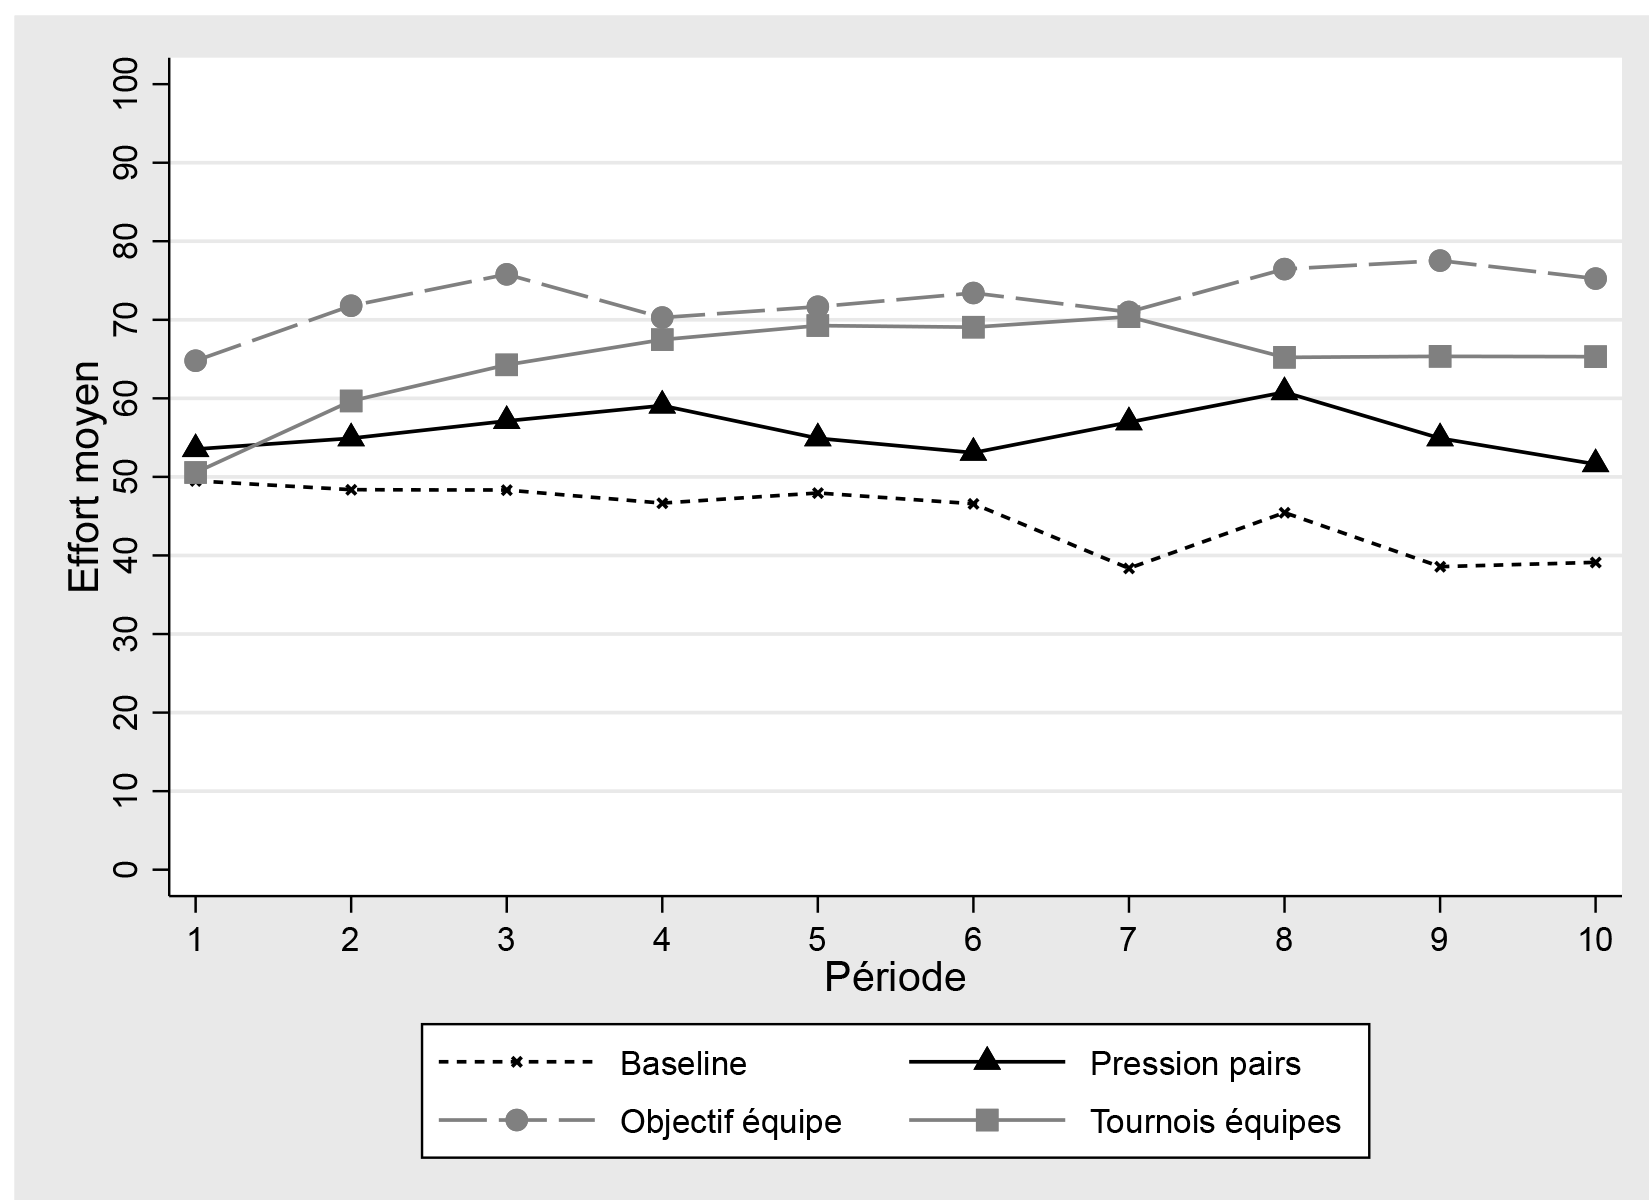
\includegraphics[height=6cm]{05_graph1.png}
\end{figure}

La figure~1 indique que l'effort moyen dans le traitement Baseline
diminue lentement au cours du temps mais reste clairement supérieur à
l'équilibre de Nash de 18,75. Ce résultat est cohérent avec les
résultats obtenus par \textcite{NalbantianSchotter1997} ainsi qu'avec
les résultats issus de la littérature sur les expériences de jeux de
contribution volontaire au financement des biens publics qui ont mis en
évidence deux régularités empiriques fortes~: 1)~les individus
contribuent en moyenne davantage que la prédiction théorique standard et
2)~le niveau moyen de contribution diminue au cours du temps lorsque le
jeu est répété à horizon fini (voir par exemple \textcite{FehrGächter2000}, \textcite{MascletNoussairTuckerVilleval2003}, \textcite{Zelmer2003}, \textcite{SeftonShuppWalker2007} et \textcite{HerrmannThoniGächter2008})\footnote{Des études ont tenté de comprendre ces résultats.
  L'explication la plus plausible repose sur la coopération
  conditionnelle, c'est-à-dire le fait que les individus seraient
  disposés à coopérer mais que cette coopération est conditionnelle à
  l'effort observé chez les autres membres du groupe, ou en fonction de
  leurs croyances concernant les décisions des autres (voir par exemple
  \textcite{KeserVanWinder2000}, \textcite{FischbacherGächter2010} et
  \textcite{ThoniVolk2018}). \textcite{FiguièresMascletWillinger2013}
  proposent une explication alternative basée sur un idéal moral kantien
  faible dans la mesure où celui-ci peut être réévalué en fonction du
  comportement passé des autres.}. La figure~1 indique aussi que le
niveau d'effort paraît plus élevé dans le traitement Pression des pairs
que dans le traitement Baseline. Enfin, l'effort se rapproche de la
solution Pareto dans les systèmes d'incitation centralisés.

Le tableau~2 fournit des statistiques descriptives concernant l'effort
moyen par traitement. Il montre que l'effort moyen dans le traitement
Objectif d'équipe (72,80) est proche de l'optimum de Pareto de 75, et
est significativement plus élevé que dans le traitement Baseline
(44,90). Un test de Mann-Whitney bilatéral sur les efforts moyens par
équipe indique que le niveau d'effort moyen dans le traitement Objectif
d'équipe est significativement plus élevé que dans le traitement
Baseline (MW bilatéral~; \emph{p}~=~0,0065). Le niveau d'effort moyen
dans le traitement Tournois entre équipes (64,66) est aussi
significativement plus élevé que dans le traitement Baseline (MW
bilatéral~; \emph{p}~=~0,016). L'effort moyen est aussi plus élevé dans
le traitement Pression des pairs (55,70) que dans le traitement
Baseline. Toutefois cette différence n'est pas statistiquement
significative (MW bilatéral~; \emph{p}~=~0,1093).

\begin{table}[h]
    \centering
    \caption{Statistiques descriptives par traitement}
\begin{tabular}{m{3.4cm}D{1cm}D{1.5cm}D{1.5cm}D{1.5cm}}
\toprule
                            & Baseline                  & Pression des pairs        & Objectif d’équipe          & Tournois entre équipes\tabularnewline
\midrule
Effort moyen                & 44,90  \varstats{24,17}   & 55,70  \varstats{23,98}   & 72,80  \varstats{22,97}    & 64,66  \varstats{26,20}\tabularnewline
Gain moyen des travailleurs & 54,29  \varstats{22,35}   & 50,11  \varstats{21,41}   & 35,58  \varstats{31,37}    & 64,18  \varstats{47,82}\tabularnewline
Profit moyen des firmes     & 474,57  \varstats{130,54} & 577,51  \varstats{110,42} & 990,88  \varstats{153,73}  & 646,78  \varstats{175,67}\tabularnewline
Richesse globale            & 908,92  \varstats{205,06} & 978,38  \varstats{163,76} & 1275,49  \varstats{191,92} & 1160,18  \varstats{209,93}\tabularnewline
Nombre de participants     & 24                        & 24                        & 24                         & 48\tabularnewline
Observations                & 240                       & 240                       & 240                        & 480\tabularnewline
\bottomrule
\end{tabular}
\notedetableau{Les nombres entre parenthèses sont des écarts types.}
\end{table}

Pour formaliser nos résultats, nous avons réalisé des régressions en
moindres carrés généralisées à effets aléatoires (RE GLS) sur les
déterminants du niveau d'effort. Nous utilisons des effets aléatoires
pour tenir compte de la dimension en panel de nos données et du fait de
l'existence d'effets fixes de traitement. Les résultats de ces
estimations sont présentés dans le tableau~3.

Ce tableau se compose de deux parties. La partie de gauche présente
des estimations sur les déterminants de l'effort. La partie de droite
réplique les estimations de la partie de gauche mais en clustérisant les
écarts types au niveau des équipes afin de contrôler les
interdépendances au sein des équipes. La colonne~1 du tableau indique
que toutes les variables de traitement ont un coefficient positif et
significatif, ce qui suggère qu'introduire un mécanisme d'incitation a
un effet positif sur le niveau d'effort par rapport au traitement de
référence de partage de revenu. La colonne~2 reproduit l'estimation~1
avec l'ajout de variables de tendance (période) et de caractéristiques
démographiques. Les effets de traitement sont robustes à l'introduction
de ces variables. La variable de tendance a un coefficient positif,
indiquant que l'effort moyen augmente au fil du temps\footnote{Notons
  toutefois que cette tendance positive cache des différences entre
  traitements. En effet, des estimations séparées par traitement
  (disponibles sur demande) révèlent une tendance positive pour les
  traitements centralisés et décentralisés, mais une tendance négative
  pour le traitement Baseline.}. La plupart des variables démographiques
sont non significatives à l'exception de la variable «Science
économiques» dont le coefficient est négatif et significatif à
10~\%\footnote{Ce résultat est cohérent avec des études antérieures
  qui ont montré que les étudiants en économie sont en moyenne plus
  enclins à adopter un comportement de passager clandestin dans les
  expériences de biens publics (\textcite{MarwellAmes1981}), et plus
  susceptibles de faire défection dans les jeux du dilemme du prisonnier
  (\textcite{FrankGilovichRegan1993}) et dans les jeux de solidarité
  (\textcite{SeltenOckenfels1998}) ou d'offrir des montants inférieurs
  dans des jeux d'ultimatum (\textcite{CarterIrons1991}). Une hypothèse
  avancée dans la littérature serait l'autosélection, suggérant que les
  individus ayant des tendances intrinsèquement égoïstes seraient plus
  susceptibles de choisir l'économie comme spécialité. Une autre
  explication alternative avance que l'enseignement de l'économie
  encouragerait les étudiants à adopter un comportement plus rationnel
  et maximisateur à l'instar de l'\emph{homo economicus} décrit dans les
  manuels de microéconomie (voir \textcite{BaumanRose2009} pour une
  discussion à ce propos).}.

\begin{table}
    \caption{Déterminants du niveau d’effort}
    \tabcolsep=2pt
    \begin{tabular}{@{}>{\raggedright}p{2cm}>{\raggedleft}p{1cm}l>{\raggedleft}p{1cm}l>{\raggedleft}p{1cm}l>{\raggedleft}p{1cm}l>{\raggedleft}p{1cm}l>{\raggedleft}p{1cm}l @{}}
    \hline
    & Tous &  & Tous &  & Tous sauf traitement & & Tous &  & Tous &  & Tous sauf traitement baseline \tabularnewline
    & & & & & & & \multicolumn{6}{c}{Avec les écarts types clusterisés} \tabularnewline
    \hline
    Var. dép.~: Niveau effort & RE GLS (1) & & RE GLS (2) & & RE GLS (3) & & & & & & & \\
    \hline
    Baseline & Réf. & & Réf. & & & & & & & & & \\
    Pression des pairs & 10,80
    \varstats{4,53} & ** & 11,01
    \varstats{4,58} & ** & Réf. & & 10,80
    \varstats{6,27} & * & 11,01
    \varstats{6,09} & * & Réf. & \\
    Objectif d'équipe & 27,90
    \varstats{4,53} & *** & 27,88
    \varstats{4,65} & *** & 16,69
    \varstats{4,73} & *** & 27,90
    \varstats{4,97} & *** & 27,88
    \varstats{4,70} & *** & 16,69
    \varstats{6,27} & *** \\
    Tournois entre équipes & 19,76
    \varstats{3,92} & *** & 19,73
    \varstats{4,11} & *** & 8,53
    \varstats{4,17} & ** & 19,76
    \varstats{4,75} & *** & 19,73
    \varstats{4,74} & *** & 8,53
    \varstats{6,25} & \\
    Période & & & 0,61
    \varstats{0,24} & ** & 1,06
    \varstats{0,26} & *** & & & 0,61
    \varstats{0,49} & & 1,06
    \varstats{0,56} & * \\
    Homme & & & --~0,17
    \varstats{3,03} & & --~0,43
    \varstats{3,49} & & & & --~0,17
    \varstats{2,35} & & --~0,43
    \varstats{2,86} & \\
    Participation antérieure & & & 3,47
    \varstats{3,69} & & 3,86
    \varstats{3,92} & & & & 3,47
    \varstats{3,57} & & 3,86
    \varstats{3,86} & \\
    Âge & & & 0,36
    \varstats{0,60} & & 0,19
    \varstats{0,77} & & & & 0,36
    \varstats{0,58} & & 0,19
    \varstats{0,88} & \\
    Sciences économiques & & & --~6,53
    \varstats{3,94} & * & --~5,93
    \varstats{4,32} & & & & --~6,53*
    \varstats{3,42} & & --~5,93
    \varstats{3,81} & \\
    Dummy Dernière période & & & --~4,39
    \varstats{2,29} & * & --~5,39
    \varstats{2,53} & ** & & & --~4,39
    \varstats{3,24} & & --~5,39
    \varstats{4,00} & \\
    Constante & 44,90
    \varstats{3,20} & *** & 35,13
    \varstats{12,71} & *** & 47,21
    \varstats{16,79} & *** & 44,90
    \varstats{3,62} & *** & 35,13
    \varstats{13,55} & ** & 47,21
    \varstats{20,91} & ** \\
    \hline
    Observations & 1200 & & 1200 & & 960 & & 1200 & & 1200 & & 960 & \\
    R-squared overall & 0,1292 & & 0,1475 & & 0,08 & & 0,1292 & & 0,1475 & &
    0,08 & \\
    Wald χ\textsuperscript{2} & 44,06 & & 56,58 & & 33,54 & & 34,28 & &
    126,18 & & 100,31 & \\ 
    \hline
    \end{tabular}
    \notedetableau{Les nombres entre parenthèses sont les écarts types. *** \emph{p}~<~0,01, ** \emph{p}~<~0,05, * \emph{p}~<~0,1.}
\end{table}

\newpage

Nous observons aussi un effet de fin de jeu, comme le montre le coefficient négatif et significatif associé à la variable dichotomique «Dernière période». La colonne~3 reproduit
l'estimation présentée dans la colonne~2 mais sur l'échantillon
restreint sans le traitement Baseline. La variable omise est alors la
variable Pression des pairs. Les variables Objectif d'équipe et Tournois
entre équipes ont un coefficient positif et significatif, montrant que
les mécanismes centralisés sont plus efficaces que le mécanisme de
Pression des pairs pour accroître le niveau d'effort. Les estimations
présentées dans la partie droite du tableau donnent des résultats
qualitativement très similaires à ceux présentés dans la partie gauche.
Une exception notable est que la variable Tournois entre équipes n'est
désormais plus significative dans l'estimation~6 après avoir clustérisé
les écarts types. Au total, nos conclusions sont présentées ci-dessous
dans le résultat~1.

% Résultat~1

\vspace{.2cm}
\begin{resultat}
a)~En l'absence de mécanisme d'incitation, le
partage des revenus induit un niveau d'effort faible mais supérieur à
celui théoriquement prévu. b)~La pression des pairs et les deux
mécanismes centralisés conduisent à des niveaux d'efforts des
travailleurs plus élevés que le traitement Baseline de partage des
revenus. c)~Les mécanismes centralisés et en particulier le mécanisme
d'objectif d'équipe génèrent des niveaux d'effort significativement plus
élevés que le mécanisme de pression des pairs.
\end{resultat}


\subsection{Analyse des sanctions dans le traitement Pression des pairs}

Dans cette sous-section, nous analysons les sanctions dans le traitement
Pression des pairs. La figure~2 montre l'évolution du nombre moyen de
points reçus au fil des périodes. Cette figure indique que le nombre de
points reçus diminue régulièrement avec le temps. Ce résultat est
cohérent avec les résultats antérieurs concernant les expériences de
biens publics avec sanction (par exemple \textcite{Nikiforakis2008}~;
\textcite{GächterRennerSefton2008}~; \textcite{MascletVilleval2008}~;
\textcite{NikiforakisEngelmann2011}~; \textcite{DickinsonMasclet2015}).
La raison souvent évoquée dans cette littérature pour expliquer cette
tendance négative est qu'après plusieurs périodes, une fois la
coopération établie au sein de l'équipe, la punition devient crédible et
n'est alors plus nécessaire pour maintenir la coopération (voir \textcite{GächterRennerSefton2008}). Cette baisse tendancielle semble davantage
résulter de la diminution du nombre de points attribués que de celle du
nombre de punisseurs, dont la proportion reste plutôt stable dans le
temps (voir figure~A1 dans l'annexe~\ref{Annexe:Éléments stats}). Il est intéressant de noter que la figure~2 montre qu'il reste un niveau de sanction substantiel
lors de la dernière période, ce qui suggère l'existence de motifs non
stratégiques pour sanctionner\footnote{Ainsi, parmi les
  24~participants du traitement Pression des pairs, 10 punissent au
  cours de la dernière période. Nous les appelons les punisseurs
  ultimes. Une description détaillée de ces punisseurs ultimes est
  présentée à l'annexe~\ref{Annexe:Éléments stats}. Nous remercions un relecteur anonyme pour
  cette suggestion utile.}.

\begin{figure}[h]
    \centering
    \caption{Évolution du nombre moyen de points reçus par travailleur}
    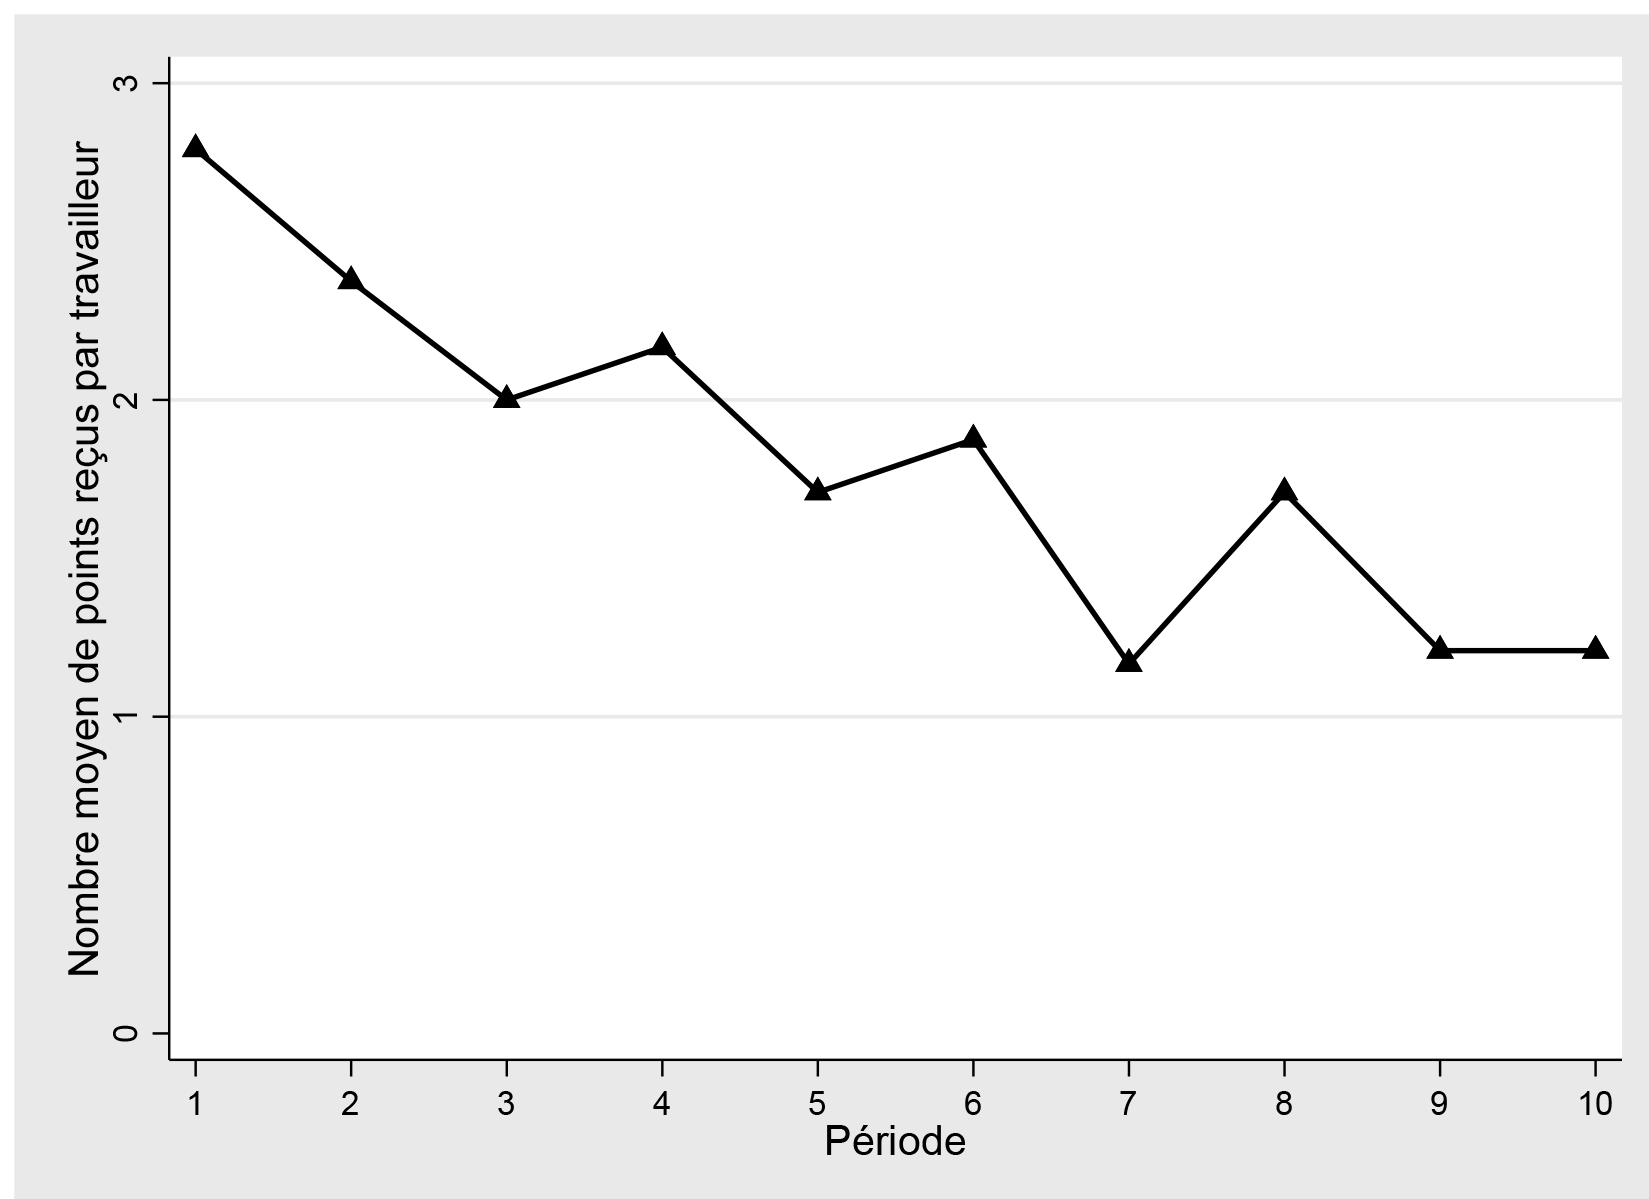
\includegraphics[height=6cm]{05_graph2.png}
\end{figure}

La figure~3 montre le nombre de points de sanction reçus par un
joueur~\emph{i} en fonction de l'écart entre l'effort du joueur~\emph{i}
et l'effort moyen des autres membres de son équipe. La figure~3
indique que davantage de points de sanction sont attribués pour des
écarts négatifs, ce qui est cohérent avec les résultats antérieurs dans
les expériences de bien public avec sanction (\textcite{FehrGächter2000}~; \textcite{MascletNoussairTuckerVilleval2003}; \textcite{HerrmannThoniGächter2008}; \textcite{MascletVilleval2008}). Mais plus
surprenant, la figure~3 indique aussi que les écarts positifs sont
également sanctionnés, bien que dans une moindre mesure. Cependant, un
tel phénomène a déjà été rapporté dans des expériences de bien public
(\textcite{FehrGächter2000}; \textcite{MascletNoussairTuckerVilleval2003}; \textcite{HerrmannThoniGächter2008}; \textcite{MascletVilleval2008}).
De telles punitions ont été classées comme «perverses» ou
«antisociales» (voir par exemple \textcite{CinyabugumaPagePutterman2006}, \textcite{HerrmannThoniGächter2008}, \textcite{NikiforakisNoussairWilkening2012}, \textcite{DenantBoemontMascletNoussair2007} et, plus récemment, \textcite{FuPutterman2018})\footnote{Des études
  ont tenté d'étudier les déterminants des punitions antisociales (voir \textcite{GächterHerrmann2009} pour une discussion détaillée).
  Certains auteurs ont mis en lumière le désir de vengeance (aveugle)
  (\textcite{DenantBoemontMascletNoussair2007}~; \textcite{Nikiforakis2008}~; \textcite{HerrmannThoniGächter2008}). D'autres études
  ont montré l'existence d'une pure volonté de nuire aux autres en
  l'absence d'avantages matériels (\emph{pure nastiness}), qui pourrait
  refléter un désir de domination (\textcite{Zizzo2003}). En outre, les
  individus peuvent manifester de l'aversion envers les coopérateurs,
  punir les non-conformistes et pénaliser les manifestations de
  générosité manifeste (\textcite{CarpenterMatthews2012}~; \textcite{Henrich2006}). D'autres études ont mis en lumière les
  différences culturelles à un niveau macro en matière de punitions
  perverses. Par exemple, \textcite{HerrmannThoniGächter2008} ont
  constaté que les sanctions antisociales ont tendance à se produire
  plus fréquemment dans les sociétés caractérisées par de faibles normes
  sociales de coopération, un faible État de droit et des démocraties
  faibles. Les sanctions antisociales semblent également être souvent
  observées dans les sociétés plus traditionnelles structurées autour de
  solides réseaux privés. Il est intéressant de noter que dans la
  littérature en gestion et économie des ressources humaines, un autre
  motif de sanction antisociale est souvent évoqué, à savoir que
  certains membres d'une équipe peuvent vouloir sanctionner les
  collaborateurs qui coopèrent, pour éviter que la firme ne révise à la
  hausse à l'avenir ses exigences telles que l'objectif à atteindre.
  Toutefois, dans le cadre de notre expérience, ce dernier motif peut
  être exclu puisque les participants étaient informés que l'objectif à
  atteindre était identique à chaque période.}.

\begin{figure}[h]
    \centering
    \caption{Points de sanction reçus et déviation à l'effort moyen des
autres}
    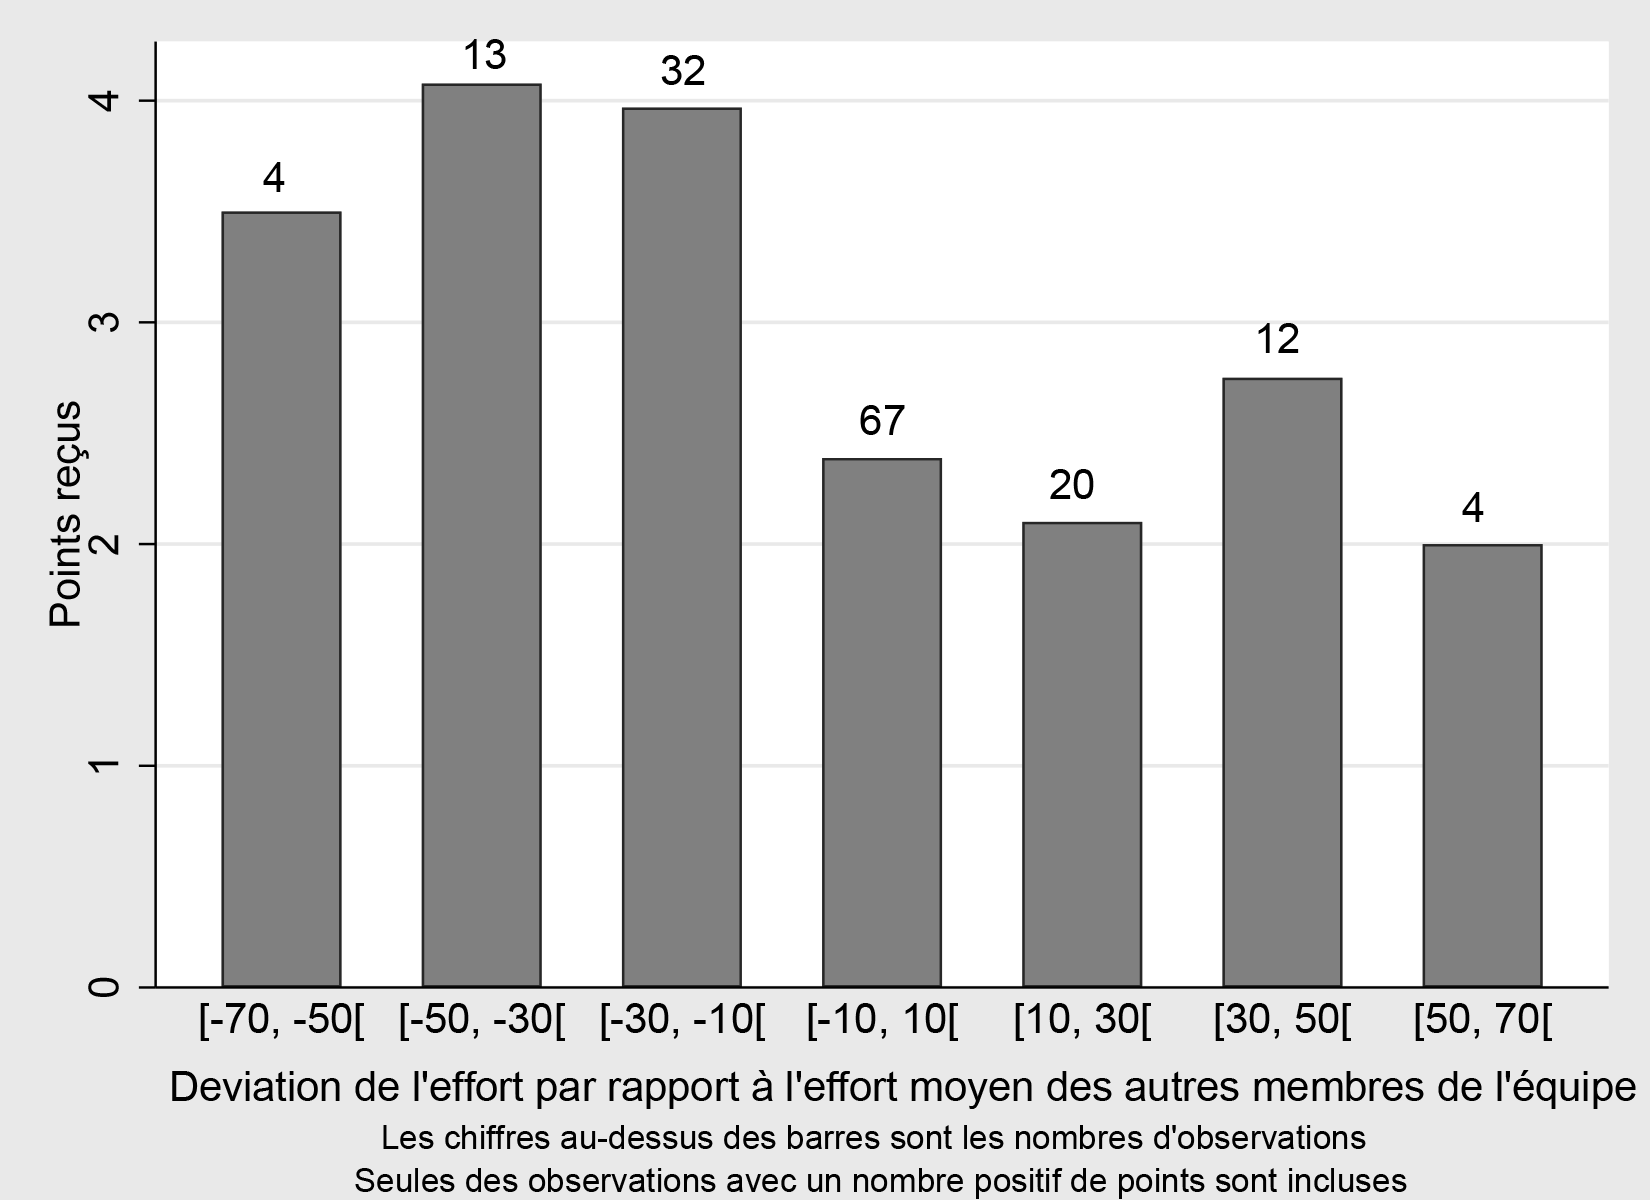
\includegraphics[height=6cm]{05_graph3.png}
\end{figure}

Le tableau~4 présente des estimations sur les déterminants des points de
sanction reçus. La variable dépendante est le nombre de points reçus. On
utilise un modèle Tobit à effet aléatoire afin de contrôler pour les
observations censurées à gauche.

\begin{table}[!ht]
    \renewcommand{\arraystretch}{1.5}
    \caption{Déterminants des points de sanction reçus}\label{tab4}
    \fontsize{8}{10}\selectfont
    \centering
    \begin{tabular}{@{}>{\raggedright}p{7cm}D{2cm}l@{}}
    \toprule
    Var. dép.~: Points de sanction reçus & \multicolumn{2}{>{\centering}p{3.5cm}}{Modèle Tobit effets aléatoires} \tabularnewline
    \midrule
    Effort moyen des autres membres de l'équipe & 0,042 \varstats{0,018} & ** \\
    Valeur absolue de déviation négative par rapport à l'effort moyen des
    autres membres de l'équipe & 0,061 \varstats{0,016} & *** \\
    Déviation positive par rapport à l'effort moyen des autres membres de
    l'équipe & 0,008 \varstats{0,017} & \\
    Période & --~0,25 \varstats{0,07} & *** \\
    Dernière période & 0,20 \varstats{0,70} & \\
    Constante & --~0,77 \varstats{1,21} & \\
    \midrule
    Observations & 240 & \\
    Non censurées & 152 & \\
    LR χ\textsuperscript{2} & 43,69 & \\
    Log Likelihood & --~416,42 &  \\
    \bottomrule
    \end{tabular}
    \notedetableau{Les chiffres entre parenthèses sont des erreurs types.
    ***~\emph{p}~\textless~0,01, **~\emph{p}~\textless~0,05,
    *~\emph{p}~\textless~0,1. La variable «Valeur absolue de déviation
    négative par rapport à l'effort moyen des autres membres de l'équipe»
    est construite comme suit~: elle prend la valeur absolue de l'écart
    négatif de l'effort du travailleur par rapport à l'effort moyen des
    autres membres de son équipe si le travailleur exerce moins d'effort que
    les autres, et zéro sinon. La variable «Déviation positive par rapport
    à l'effort moyen des autres membres de l'équipe» est construite comme
    suit~: elle prend la valeur de l'écart positif de l'effort du
    travailleur par rapport à l'effort moyen des autres au sein de son
    équipe, si le travailleur exerce un effort plus élevé que les autres, et
    zéro autrement.}
    \end{table}

La variable «Valeur absolue de déviation négative par rapport à
l'effort moyen des autres membres de l'équipe» a un coefficient positif
et significatif, indiquant que les travailleurs reçoivent davantage de
sanctions de la part de leurs pairs lorsqu'ils choisissent des efforts
inférieurs à la moyenne de leurs pairs. En revanche, la variable
«Déviation positive par rapport à l'effort moyen des autres membres de
l'équipe» n'est pas significative. La variable «Période» est négative
et significative, indiquant que le nombre de points reçus diminue au fil
du temps. La variable «Dernière période» n'est pas statistiquement
significative, ce qui montre l'absence d'effet de fin de partie. Nos
conclusions sur les comportements de sanction sont résumées dans le
résultat~2.

% Résultat~2.
\vspace{.2cm}
\begin{resultat}
a)~La plupart des points de sanction sont attribués
aux travailleurs fournissant un effort inférieur à la moyenne de leur
équipe. b)~Les sanctions diminuent avec le temps. 
\end{resultat}

\newpage

\subsection{Les gains des travailleurs}

La figure~4 présente l'évolution des gains moyens des travailleurs
par traitement.

\begin{figure}[h]
    \centering
    \caption{Évolution des gains moyens des travailleurs}
    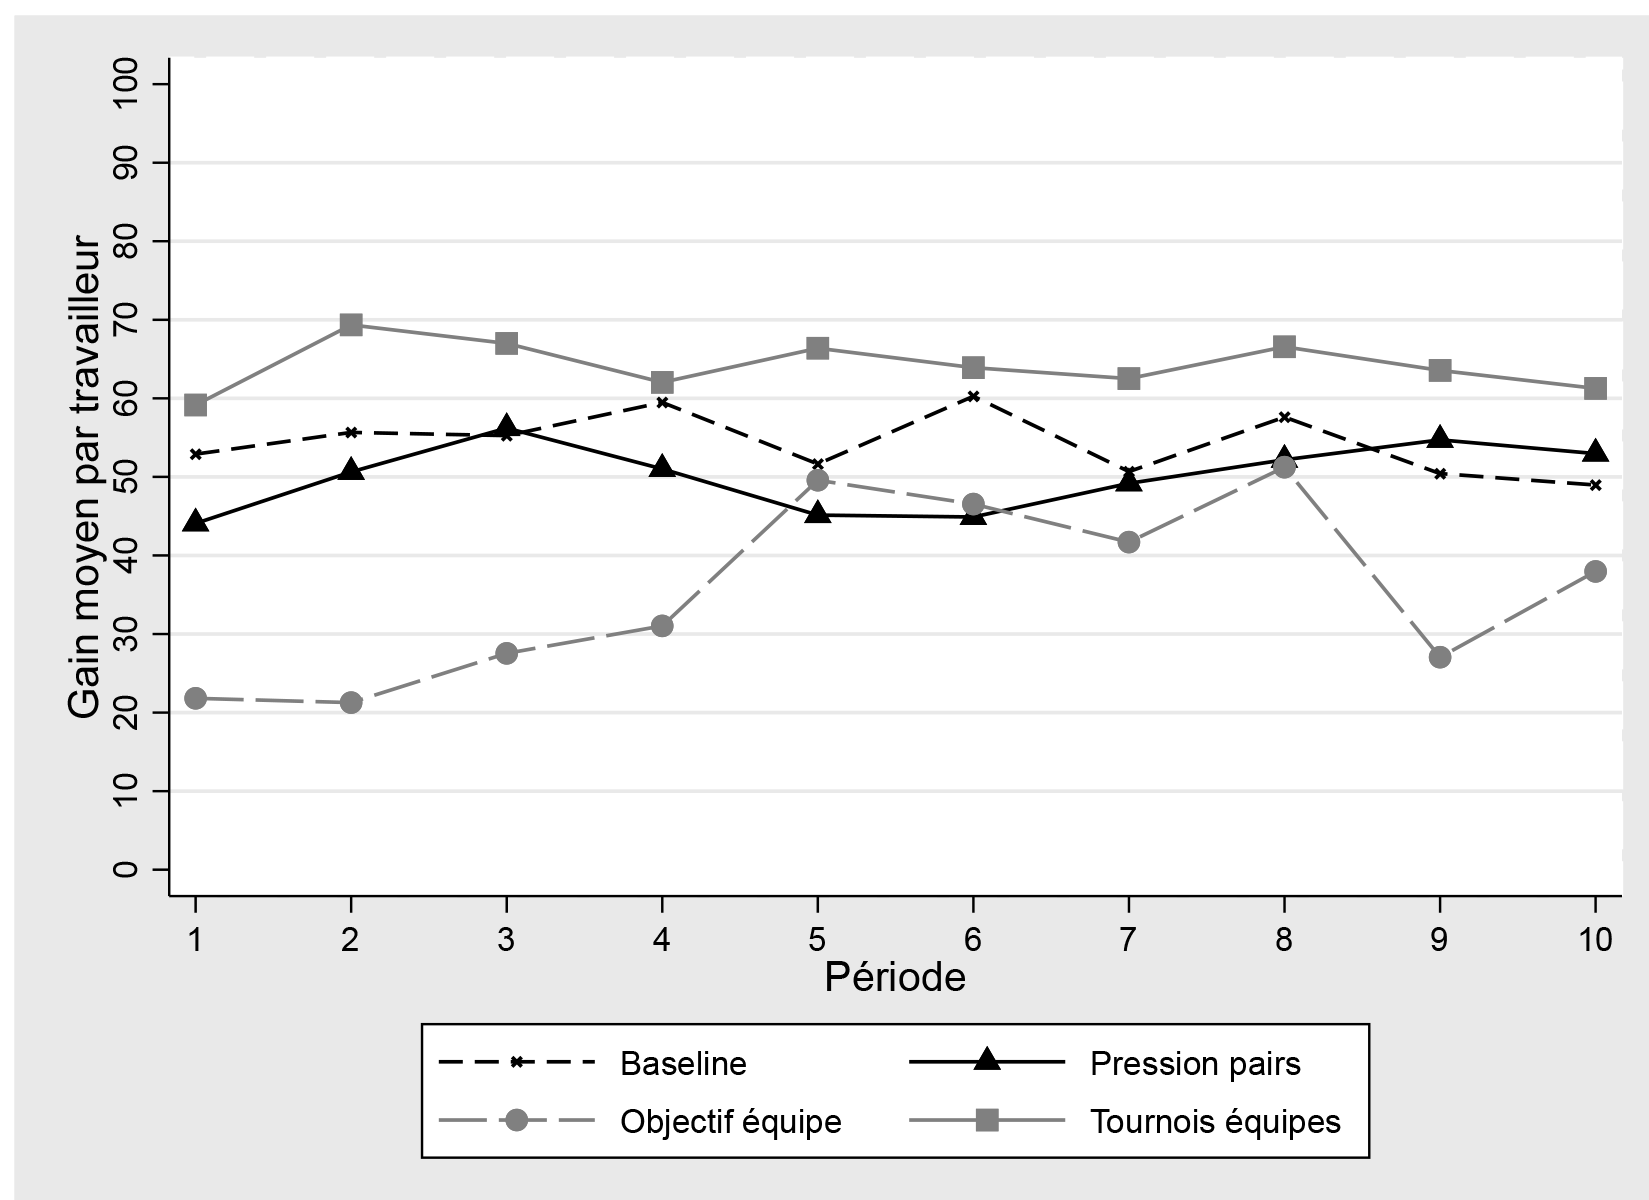
\includegraphics[height=6cm]{05_graph4.png}
\end{figure}

La figure~4 indique que le traitement Objectif d'équipe génère les
gains moyens des travailleurs les plus bas pour presque toutes les
périodes. À l'opposé, les gains sont les plus élevés dans le traitement
Tournois entre équipes. Ces résultats sont confirmés par le tableau~2.
Un test bilatéral de Mann-Whitney indique que les gains des travailleurs
sont significativement inférieurs avec le traitement Objectif d'équipe
qu'avec le traitement Baseline (\emph{p}~=~0,0065). Les gains des
travailleurs sont légèrement plus élevés dans le traitement Tournois
entre équipes que dans le traitement Baseline (\emph{p}~=~0,0547).
Enfin, selon le même test de Mann-Whitney, nous ne pouvons pas rejeter
l'hypothèse nulle selon laquelle les niveaux de gains sont les mêmes
dans le traitement Pression des pairs et dans le traitement Baseline
(\emph{p}~=~0,42). Notons que le tableau~2 fait aussi apparaître des
différences dans les écarts types de gains entre les traitements. En
particulier, l'écart type des gains des travailleurs est plus élevé dans
les systèmes d'incitation centralisés, notamment celui avec Tournois
entre équipes, comparé au traitement Baseline et à la Pression des
pairs. Cela peut s'expliquer par le dispositif de Tournois entre équipes
lui-même, qui impose des transferts entre équipes perdantes et gagnantes
à chaque période, à l'origine d'inégalités considérables de gains.

Le tableau~5 présente les résultats d'estimations sur les déterminants
des gains des travailleurs, des profits des firmes et de la richesse
totale (la somme des profits de la firme et des gains des travailleurs).

\begin{table}
    \caption{Déterminants des gains des travailleurs, des profits des firmes et de la richesse totale (RE GLS)}
\begin{tabular}{@{}L{2.4cm}D{1.8cm}L{0.5cm}D{1.5cm}L{0.5cm}D{1.5cm}L{0.5cm}@{}}
\hline
Var. dép. :              & \multicolumn{2}{>{\centering}m{1.8cm}}{Gains des travailleurs

    (1)}                 & \multicolumn{2}{>{\centering}m{1.5cm}}{Profits des firmes

    (2)}                 & \multicolumn{2}{>{\centering}m{1.5cm}}{Richesse totale

    (3)}\\\midrule
Baseline                 & Réf.                                                  & ~   & Réf.                      & ~   & Réf.                      & ~\\
Pression des pairs       & – 5,88  \varstats{4,34}                               & ~   & 102,94  \varstats{68,82}  & ~   & 69,46  \varstats{99,90}   & ~\\
Objectif d’équipe        & – 22,21  \varstats{5,64}                              & *** & 516,31  \varstats{70,04}  & *** & 366,58  \varstats{110,99} & ***\\
Tournois entre équipes   & 6,11  \varstats{4,45}                                 & ~   & 172,21  \varstats{70,55}  & **  & 251,27  \varstats{99,65}  & **\\
Période – Tendance       & 0,58  \varstats{0,46}                                 & ~   & 4,21  \varstats{6,77}     & ~   & 8,84  \varstats{7,98}     & ~\\
Homme                    & – 5,44  \varstats{3,52}                               & ~   & ~                         & ~   & ~                         & ~\\
Participation antérieure & 9,78  \varstats{6,14}                                 & ~   & ~                         & ~   & ~                         & ~\\
Âge                      & – 0,019  \varstats{0,50}                              & ~   & ~                         & ~   & ~                         & ~\\
Sciences économiques     & 4,73  \varstats{6,41}                                 & ~   & ~                         & ~   & ~                         & ~\\
Dummy Dernière période   & – 4,20  \varstats{4,59}                               & ~   & – 58,34  \varstats{51,31} & ~   & – 91,92  \varstats{65,16} & ~\\
Constante                & 53,61  \varstats{11,61}                               & *** & 457,25  \varstats{65,43}  & *** & 869,49  \varstats{96,55}  & ***\\\midrule
Observations             & 1200                                                  & ~   & 150                       & ~   & 150                       & ~\\
R-squared Overall        & 0,0951                                                & ~   & 0,5786                    & ~   & 0,3331                    & ~\\
Wald $\chi $2            & 339,94                                                & ~   & 74,98                     & ~   & 21,31                     & ~\\\bottomrule
\end{tabular}

\notedetableau{Les chiffres entre parenthèses sont des erreurs types. *** \emph{p}~<~0,01, ** \emph{p}~<~0,05, * \emph{p}~<~0,1. Les erreurs
standards sont clusterisées au niveau du groupe.}
\end{table}

La colonne~1 du tableau~5 indique que la pression des pairs n'augmente
pas significativement les gains des travailleurs. Cela peut résulter des
coûts associés aux sanctions, préjudiciables aux gains des travailleurs
et qui peuvent annuler les bénéfices d'une plus grande coopération. La
variable Tournois entre équipes est également non significative. Une
raison possible est que si ce mécanisme incite les travailleurs à
surperformer, il n'y a cependant finalement qu'une seule équipe
gagnante. Enfin, la variable Objectif d'équipe a un coefficient négatif
et significatif, indiquant que les gains des travailleurs dans ce
traitement sont significativement inférieurs à ceux obtenus dans le
traitement Baseline. Une explication possible est que plusieurs équipes
échouent à atteindre l'objectif, ce qui conduit dans ce cas à des gains
faibles. La figure~5 confirme cette intuition. Elle montre que la
proportion des équipes atteignant l'objectif dans ce traitement est
assez faible, en particulier pendant les premières périodes de jeu.
Cependant, la figure~5 indique également une évolution faible mais
positive de la proportion d'équipes qui atteignent l'objectif au cours
du temps, ce qui suggère l'absence de résignation de la part des
travailleurs. Ce constat est détaillé dans l'annexe~\ref{Annexe:Éléments stats}, dans la sous-section~\ref{Annexe:Évolution dispersion des efforts} qui étudie l'évolution de la dispersion des efforts dans le traitement Objectif d'équipe, pour les équipes qui
atteignent l'objectif, comme pour les équipes qui échouent à l'atteindre.

\begin{figure}[h]
    \centering
    \caption{Proportion d'équipes atteignant l'objectif dans le
traitement Objectif d'équipes}
    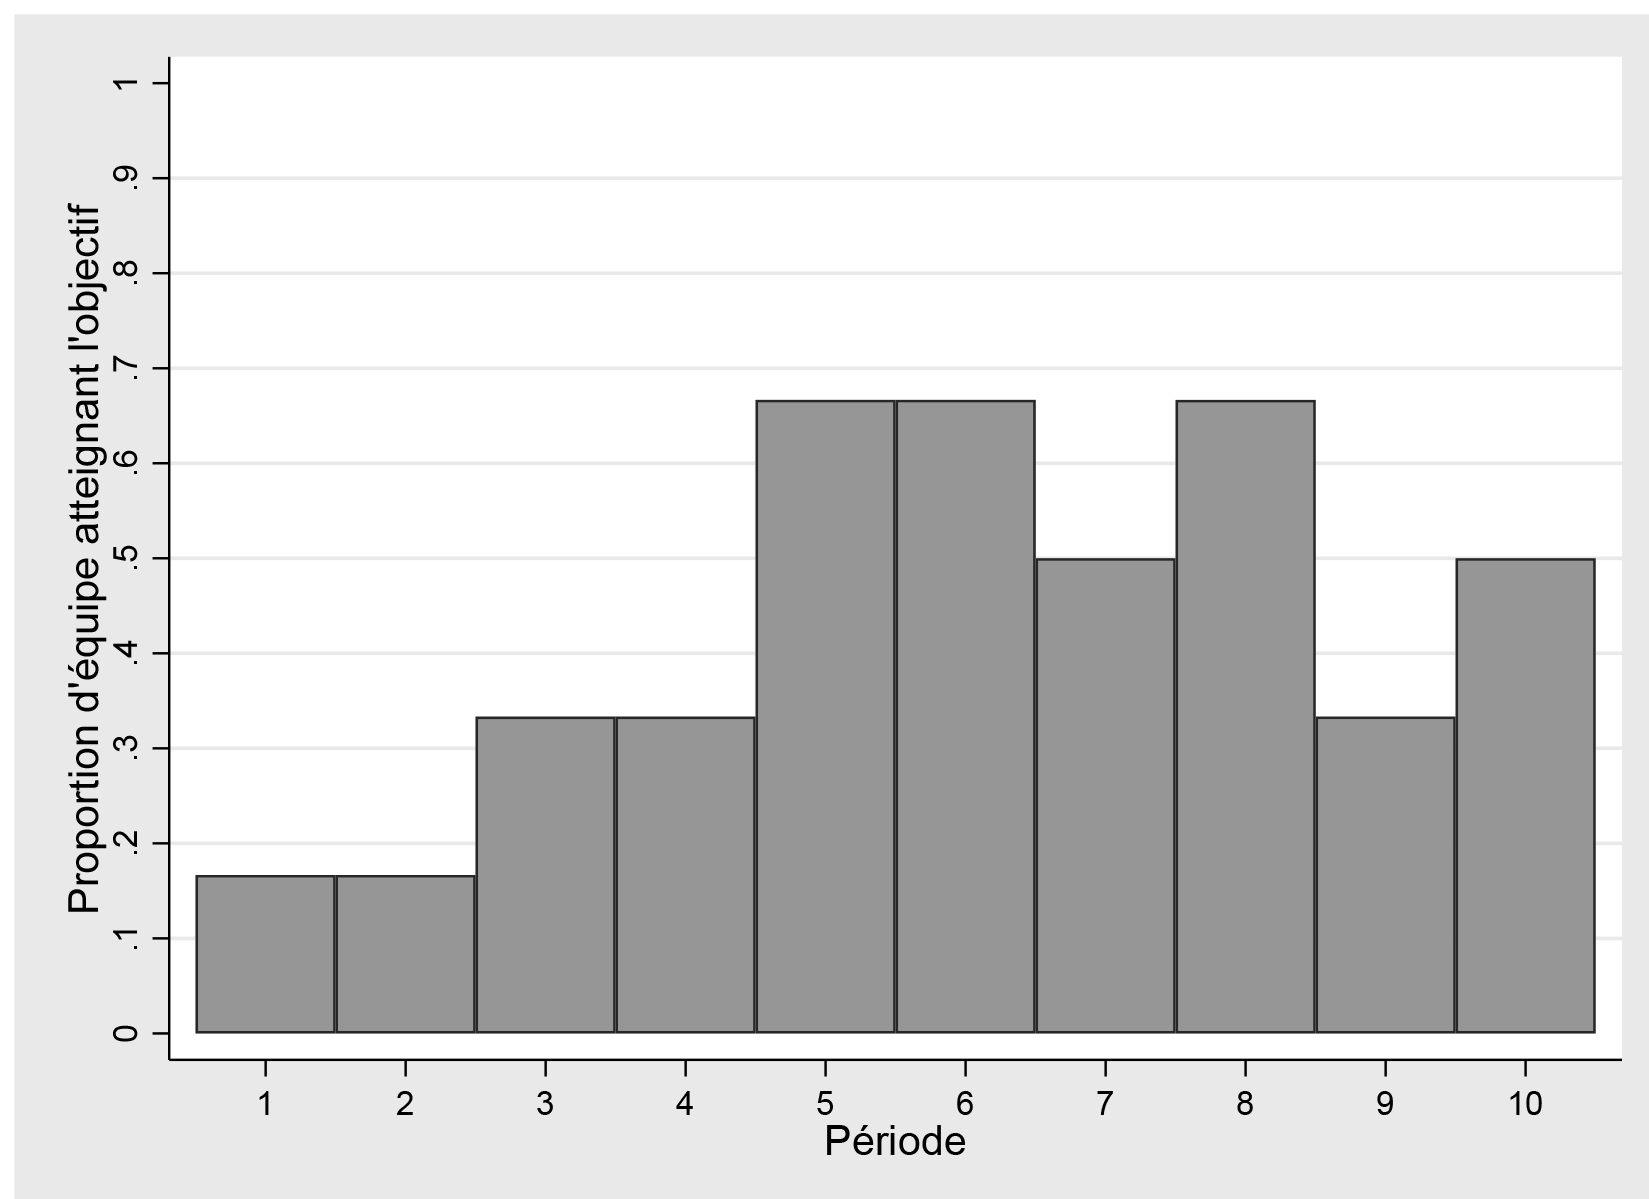
\includegraphics[height=6cm]{05_graph5.png}
\end{figure}

Au total, nos conclusions concernant les gains des travailleurs sont
résumées dans le résultat~3.

\newpage

% Résultat~3
\vspace{.2cm}
\begin{resultat}
a)~La pression des pairs n'améliore pas
significativement les gains moyens des travailleurs par rapport au
traitement Baseline, en raison du coût social des sanctions qui annule
l'effet positif de la pression par les pairs se traduisant par une
coopération accrue. b)~Le mécanisme de tournois entre équipes n'accroît
pas significativement les gains des travailleurs, par rapport au
traitement Baseline, mais augmente considérablement leur dispersion.
c)~Dans le traitement Objectif d'équipe, les gains des travailleurs sont
beaucoup plus faibles et plus dispersés que dans le traitement Baseline,
car de nombreuses équipes échouent à atteindre l'objectif.
\end{resultat}


\subsection{Les profits des firmes}

La figure~6 ci-dessous montre l'évolution du profit moyen des firmes,
par traitement. Le tableau~2 et la figure~6 montrent que les profits
des firmes sont les plus élevés dans le traitement Objectif d'équipe et
les plus faibles dans le traitement Baseline.

\begin{figure}[h]
    \centering
    \caption{Évolution du profit moyen des firmes}
    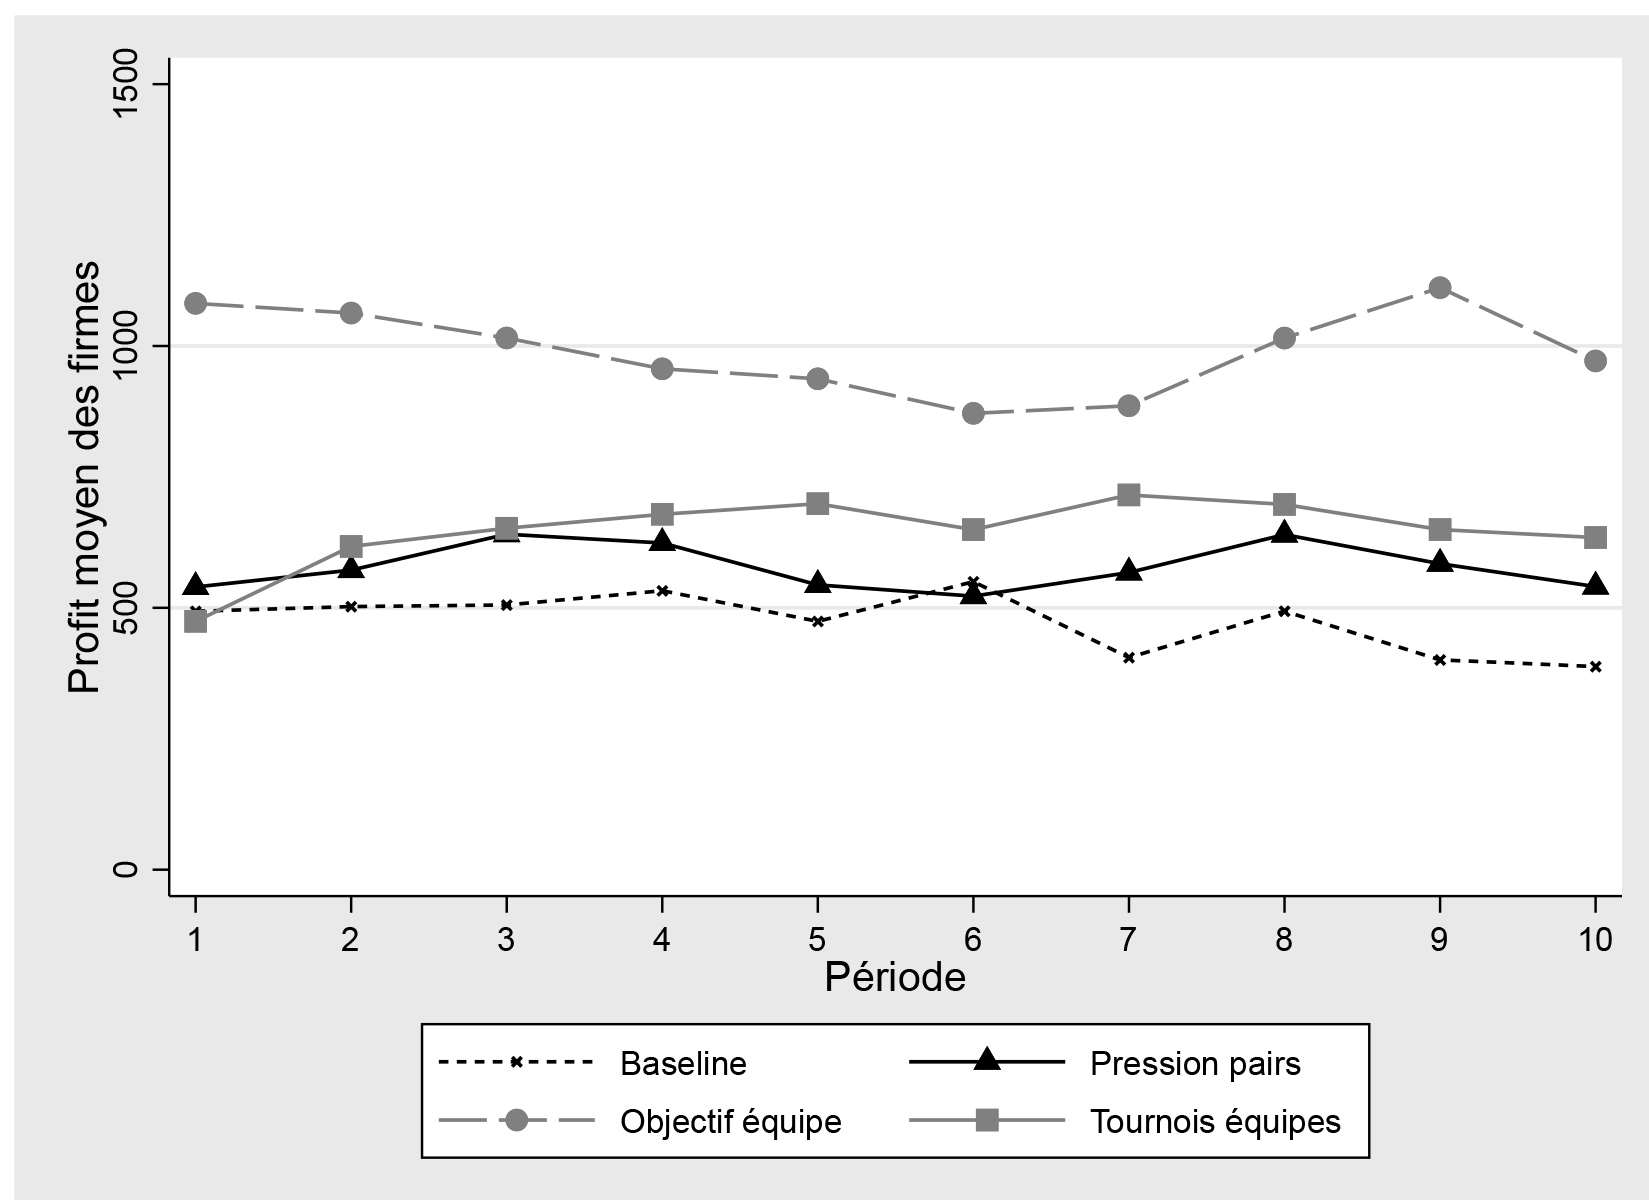
\includegraphics[height=6cm]{05_graph6.png}
\end{figure}

La colonne~2 du tableau~5 présente les résultats d'une estimation des
déterminants du profit des entreprises. Cette estimation indique que les
profits des firmes sont significativement plus élevés dans le traitement
Objectif d'équipe et, dans une moindre mesure, dans le traitement
Tournois entre équipes, comparés au traitement Baseline. La variable
Pression des pairs n'est pas significative, ce qui montre que ce
mécanisme n'améliore pas significativement les profits des firmes. Les
tests effectués sur les coefficients de la colonne~2 du tableau~5,
présentés dans la sous-section~\ref{Annexe:Significativité différences de profits} de l'annexe~\ref{Annexe:Éléments stats}, révèlent que
les profits des firmes sont significativement plus élevés dans le
traitement Objectif d'équipe que dans les traitements Pression des pairs
et Tournois entre équipes, mais qu'il n'y a pas de différence
significative de profits des firmes entre Pression des pairs et Tournois
entre équipes.

Nos conclusions concernant les profits des firmes sont présentées dans
le résultat~4.

% Résultat~4.
\vspace{.2cm}
\begin{resultat}
a)~Introduire un mécanisme centralisé augmente les
profits des firmes par rapport au traitement Baseline. b)~Les profits
des firmes sont les plus élevés avec le traitement Objectif d'équipe.
c)~La pression des pairs n'entraîne pas d'augmentation de profits des
firmes par rapport au traitement Baseline.
\end{resultat}

\subsection{À qui profite principalement l'introduction de mécanismes
(dé)centralisés~: la firme ou les travailleurs~?}

Dans cette section, nous examinons qui bénéficie principalement de
l'introduction de mécanismes (dé)centralisés. À cette fin, nous
considérons la richesse totale comme la somme des profits de la firme et
des gains des travailleurs et étudions comment elle est partagée entre
les deux parties.
Le tableau~2 plus haut montre la richesse par traitement. Il indique que
la richesse est la plus faible dans le traitement Baseline et la plus
élevée dans le traitement Objectif d'équipe, où le profit élevé des
firmes fait plus que compenser les faibles gains des travailleurs.
La colonne~3 du tableau~5 montre que la richesse totale est maximale
avec les mécanismes centralisés. Le mécanisme décentralisé de Pression
des pairs n'a pas d'effet significatif sur la richesse totale comparé au
traitement Baseline. Les tests sur les coefficients de la colonne~3 du
tableau~5, présentés dans la sous-section~\ref{Annexe:Significativité différences de profits} de l'annexe~\ref{Annexe:Éléments stats}, confirment que la richesse totale est significativement plus élevée dans
les traitements Objectif d'équipe et Tournois entre équipes que dans le
traitement Pression des pairs, mais que la différence entre les
traitements Objectif d'équipe et Tournois entre équipes n'est pas
significative.
La figure~7 montre la composition de la richesse totale par
traitement. Il indique que cette composition diffère fortement entre
traitements, soulignant les arbitrages et les aspects politiques
associés au choix d'un traitement (voir les figures~A8-A11 dans
l'annexe~\ref{Annexe:Éléments stats} pour une analyse séparée par traitement sur les évolutions de la composition de la richesse totale au fil des périodes). La
figure~7 montre qu'alors que la richesse totale est partagée presque
à égalité entre la firme et les travailleurs dans le traitement Baseline
et, dans une certaine mesure, dans les traitements Pression des pairs et
Tournois entre équipes, à l'inverse, cette répartition est nettement en
faveur de la firme dans le traitement Objectif d'équipe.

\begin{figure}[h]
    \centering
    \caption{Composition de la richesse totale}
    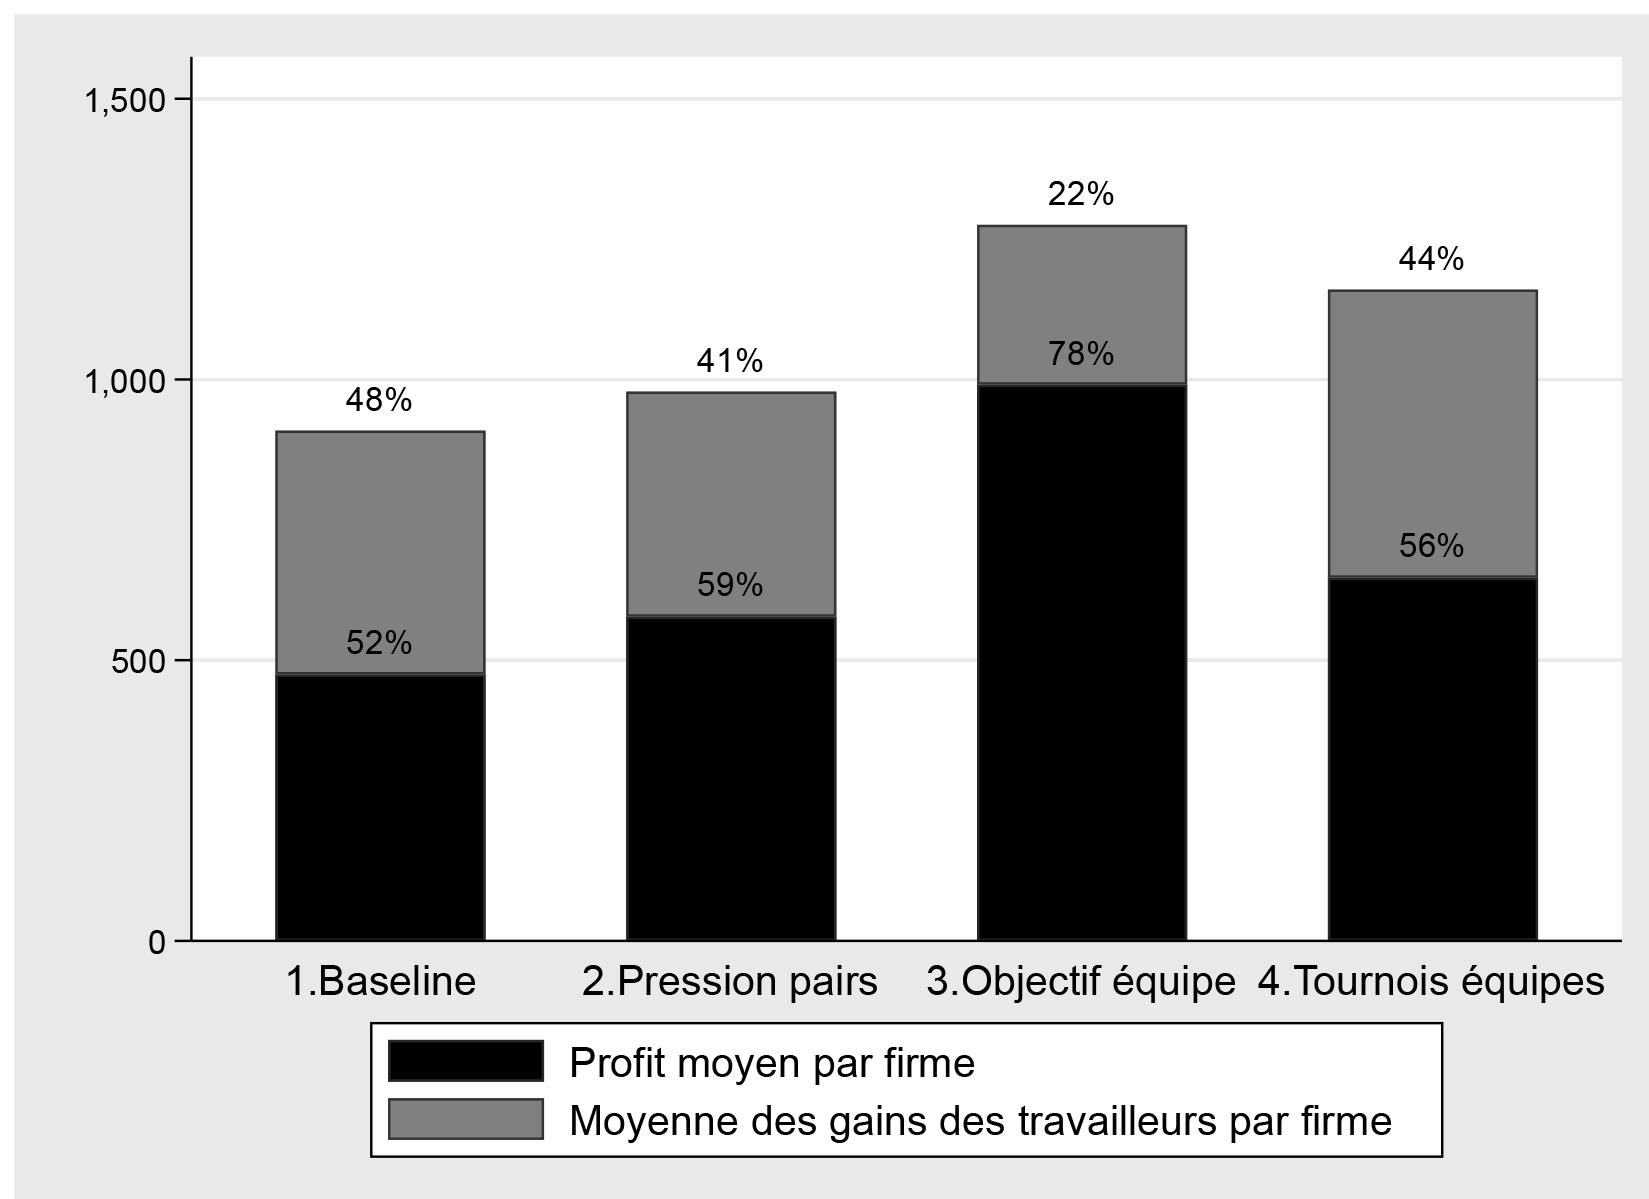
\includegraphics[height=5.5cm]{05_graph7.png}
\end{figure}

Nos principales conclusions concernant la répartition de la richesse
totale entre firme et travailleurs se résument comme suit~:

% Résultat~5.
\vspace{.2cm}
\begin{resultat}
a)~La richesse totale (c'est-à-dire la somme des
profits de la firme et des gains des travailleurs) est plus élevée avec
les mécanismes centralisés qu'avec le traitement Baseline. b)~Dans le
mécanisme avec Objectif d'équipe, les firmes captent la plus grande part
de la richesse totale. c)~La pression des pairs n'augmente pas de
manière significative la richesse totale par rapport au traitement
Baseline.
\end{resultat}


\section{Discussion et conclusion}
\label{section:discussion et conclusion}

Nous avons étudié l'efficacité et l'efficience de différents mécanismes
visant à dissuader les comportements de passager clandestin au sein
d'équipes de travail, en comparant les systèmes centralisés (basés sur
des objectifs et tournois d'équipes) et décentralisés (pression des
pairs).

Nos résultats montrent premièrement qu'en l'absence de mécanismes
d'incitation, l'effort est sujet à un phénomène de passager clandestin,
bien que moins sévère que ne le prédit la théorie.

Deuxièmement, en conformité avec les résultats obtenus précédemment dans
des expériences de contribution volontaire au financement de biens
publics avec sanction, nous observons que la pression des pairs accroît
l'effort par rapport au traitement Baseline. Toutefois, son impact reste
faible et les gains des travailleurs ne sont pas augmentés par rapport
au traitement Baseline. La raison à cela est que les coûts associés aux
sanctions annulent les gains d'une coopération accrue engendrée par la
pression des pairs.

Troisièmement, les mécanismes centralisés sont plus efficaces que la
pression des pairs pour accroître l'effort. En particulier, le mécanisme
d'objectif d'équipe conduit à un niveau d'effort proche du niveau
optimal de Pareto, mais au prix de gains plus faibles et plus inégaux
pour les travailleurs. En effet, de nombreuses équipes échouent souvent
à atteindre l'objectif. À l'opposé, ce système conduit à une forte
augmentation des profits des firmes.

Quatrièmement, la mise en place de tournois entre équipes accroît
significativement les niveaux d'effort, mais sans augmenter
significativement les gains moyens des travailleurs, et cela entraîne de
grandes inégalités de gains entre travailleurs du fait des transferts
entre équipes gagnantes et équipes perdantes.

Cinquièmement, la richesse totale est maximisée avec les mécanismes
centralisés, et en particulier avec le mécanisme d'Objectif d'équipe.
Cependant, avec ce mécanisme, la richesse est très inégalement partagée
entre la firme et les travailleurs, la première en recevant la plus
grande part.

Globalement, ces résultats mettent en lumière le fait qu'il est
important, lorsque l'on envisage la mise en place d'un système de
rémunération, de prendre en compte plusieurs dimensions dont
l'efficacité, l'efficience, mais également la manière dont la richesse
est partagée entre les parties prenantes, au risque sinon de générer des
tensions sources d'inefficiences futures. En effet, si deux mécanismes
peuvent aboutir à des niveaux similaires de richesse, l'un mettant
l'accent sur des profits plus élevés et l'autre donnant la priorité à
des gains substantiels pour les travailleurs, la décision sur le
mécanisme à mettre en œuvre peut nécessiter un arbitrage politique
nuancé\footnote{Nous remercions ici un évaluateur anonyme pour cette
  remarque pertinente.}.

Notre étude a bien sûr des limites et peut susciter certaines
interrogations. Une première interrogation porte sur la validité externe
de nos résultats. Ainsi, dans quelle mesure ceux-ci peuvent-ils
être étendus à d'autres populations et d'autres contextes du monde réel,
au-delà du laboratoire~? On peut en effet raisonnablement douter de la
possibilité d'extrapoler des résultats de laboratoire, qui constitue un
environnement pouvant être perçu comme artificiel et manquant de
réalisme (voir par exemple \textcite{BerkowitzDonnerstein1982} et
\textcite{Colquitt2008}). En outre, on peut se demander si un petit nombre
de participants, étudiants pour la plupart, sont représentatifs de
populations plus larges (\textcite{LevittList2007}, \textcite{LevittList2007-1}).
Répondre à cette question nécessite d'abord de définir la notion de
validité externe. À l'instar de \textcite{KesslerVesterlund2015} et
\textcite{LevittList2007}, il convient de distinguer entre validité
externe quantitative et qualitative. En effet, si nos résultats ne
peuvent prévoir la magnitude des effets considérés (faible validité
externe quantitative), ils peuvent néanmoins avoir une bonne validité
externe qualitative ou directionnelle, c'est-à-dire donner une certaine
indication sur la direction de l'effet considéré\footnote{Cela a été
  joliment résumé par \textcite{LevittList2007}, p.~351, dans les
  termes suivants~: «\emph{It is likely that the qualitative findings
  of the lab are generalizable, even when the quantitative magnitudes
  are not}.» La distinction entre résultats quantitatifs et qualitatifs
  est fortement liée à la question de la validité externe des résultats
  expérimentaux. Les résultats quantitatifs font référence à
  l'«ampleur» ou à la «magnitude» d'un effet tandis que les
  résultats qualitatifs font référence à la «direction» d'un effet.}.
En d'autres termes, la question n'est pas de savoir dans quelles
proportions les mécanismes centralisés surpassent le système
décentralisé mais de savoir quelle est la direction de l'effet. Le
critère d'évaluation de la validité externe doit se concentrer sur la
question de savoir si le signe de l'effet reste cohérent dans différents
environnements. De plus, notre expérience doit être considérée comme une
première étape qui appelle à être reproduite (\textcite{Camerer2015}).
Lorsqu'un effet a été reproduit dans l'environnement contrôlé du
laboratoire, et dans un cadre bien défini, son ampleur peut être alors
évaluée sur le terrain et dans le contexte souhaité. \textcite{Schram2005},
p.~232, discute de ce point en utilisant l'analogie avec les tests d'un
nouvel avion en soufflerie~: «\emph{After a theoretical design, a test}
[of a new airplane] \emph{in a wind tunnel is the stage of
laboratory experimentation. If it does not ``crash'' in this experiment,
the plane is not immediately used for the transport of passengers,
however. One will typically conduct further tests in the wind tunnel
under extreme circumstances. In addition, further testing including
``real'' flights without passengers will be conducted.~}»

Une extension naturelle de notre étude consisterait à tester si des
professionnels présenteraient un comportement similaire à la fois en
laboratoire et dans leur contexte de travail (\textcite{HarrisonList2004} appellent de telles expériences des expériences
artefactuelles de terrain de type «\emph{lab in the field}» ou
«\emph{field in the lab}»). Cela nous permettrait de vérifier si nos
résultats sont valables dans d'autres environnements, et d'accroître
ainsi leur validité externe.

Une autre piste de recherche consisterait à mener des traitements
supplémentaires visant à dissocier les effets de réputation des effets
des mécanismes incitatifs\footnote{Nous remercions un rapporteur
  anonyme pour cette suggestion.}. Par exemple, comparer nos traitements
selon que la composition des équipes reste inchangée au cours du temps
(«\emph{Partner matching}») ou qu'elle change à chaque période
(«\emph{Stranger marching}») permettrait d'identifier d'éventuels
effets réputationnels. Une autre piste d'extension consisterait
également à enrichir notre cadre théorique en considérant le rôle de
l'aversion au risque, des préférences sociales (voir \textcite{FehrSchmidt1999}) ou des intentions (\textcite{Rabin1993}). Enfin, une extension
de nos travaux consisterait à chercher à rendre la pression des pairs
plus efficace. Ainsi sa performance serait-elle améliorée si cette
pression était centralisée entre les mains d'un leader d'équipe~?

{\sloppy % Justification du texte plus "laxiste"
\printbibliography
}

\newpage

\begin{appendices}

%ANNEXES

\section{Prédictions théoriques}
\label{Annexe:Prédictions}

\subsection{Traitement Baseline}
\label{Annexe:Traitement Baseline}

\vspace{0,3cm}
Dans le traitement Baseline, le gain de chaque membre~\emph{i} de
l'équipe~\emph{j},\emph{π\textsubscript{i}}\textsubscript{,\emph{j}},
est donné par~:
\begin{equation}
    \frac{\pi_{i,j} = 1,5\left( \sum_{1}^{4}e_{i,j} + \varepsilon \right)}{4} - \left( \frac{e_{i,j}^{2}}{100} \right) + 10.
\end{equation}

Avec la condition de premier ordre~:
\begin{equation}
  \frac{\partial\pi_{i,j}}{\partial e_{i,j}} = \frac{1,5}{4} - \frac{2e_{i,j}}{100} = 0.
\end{equation}

On déduit facilement des équations~(A1) et (A2) que les gains de
\emph{i} sont maximisés pour l'effort \(e_{ij}^{*} = 18,75\), qui
correspond à l'équilibre de Nash de ce jeu. Cet effort est en dessous du
niveau d'effort Pareto-optimal de 75. Le jeu étant répété un nombre fini
de fois, le seul équilibre parfait en sous-jeux du jeu, consiste pour
tous les joueurs à fournir un effort \(e_{ij}^{*} = 18,75\) à chaque
période.

Les prédictions théoriques précédentes reposent sur l'hypothèse standard
que les individus poursuivent uniquement leur intérêt matériel
personnel, étant dépourvus de préférences sociales. Or plusieurs
résultats empiriques suggèrent que cette hypothèse ne se vérifie pas
toujours. Par exemple, dans un contexte similaire de jeu d'effort avec
partage de revenus, \textcite{NalbantianSchotter1997} observent que le
niveau d'effort se maintient au-dessus du niveau de l'équilibre de Nash
tout en diminuant toutefois au cours du temps. Ces résultats sont
également cohérents avec la littérature sur les expériences de biens
publics qui a documenté deux fortes régularités empiriques~: 1)~le fait
que les individus contribuent plus que ce que prédit le modèle théorique
standard au bien public~; et 2)~que cette contribution moyenne diminue
au cours du temps lorsque le jeu est répété sur un horizon fini (voir \textcite{Ledyard1995}, \textcite{Andreoni1995}, \textcite{Croson1996}, \textcite{KeserVanWinder2000}, \textcite{FehrGächter2000}, \textcite{MascletNoussairTuckerVilleval2003}, \textcite{HerrmannThoniGächter2008}, \textcite{KriegSamek2017}). La littérature propose trois explications majeures à ces
phénomènes~: les effets d'apprentissage (\textcite{Andreoni1988})\footnote{L'hypothèse d'effets d'apprentissage postule que
  les contributions initiales élevées proviennent de la confusion et des
  erreurs des sujets, diminuant progressivement à mesure qu'ils
  identifient la possibilité d'obtenir des gains plus élevés avec des
  contributions réduites. Toutefois l'hypothèse d'effets d'apprentissage
  semble incompatible avec l'«effet de \emph{restart}» (voir \textcite{Andreoni1988}).}, les comportements stratégiques (\textcite{KrepsMilgromRobertsWilson1982})\footnote{L'hypothèse de comportement stratégique, ancrée
  dans l'hypothèse du «\emph{crazy player}» (\textcite{KrepsMilgromRobertsWilson1982}), ou l'absence de connaissance commune de la rationalité,
  postule que si les acteurs rationnels croient qu'il existe un
  \emph{crazy player} dans le groupe, contribuant positivement au cours
  de la période~1, alors il devient rationnel pour eux d'adopter une
  stratégie coopérative au début, en diversifiant les stratégies au fur
  et à mesure de la progression du jeu répété. Cependant, les résultats
  d'\textcite{Andreoni1988} tendent à remettre en question cette hypothèse
  en tant qu'explication plausible de la diminution de la contribution
  moyenne.} et la coopération conditionnelle (\textcite{FischbacherGächterFehr2001}). Alors que les résultats empiriques suggèrent que
l'apprentissage ou les comportements stratégiques ne jouent qu'un rôle
limité dans l'explication de la baisse du niveau de contribution, la
plupart des études ont concentré leur attention sur le rôle joué par la
coopération conditionnelle, c'est-à-dire le fait que les individus
conditionnent leurs comportements sur l'observation du comportement des
autres, ou sur leurs croyances concernant le comportement des autres,
dans des jeux de bien public simultanés et répétés de manière finie (par
exemple \textcite{KeserVanWinder2000}, \textcite{FischbacherGächterFehr2001}, \textcite{Croson2007} et \textcite{FischbacherGächter2010}).
D'autres travaux ont avancé l'hypothèse de coopération conditionnelle
imparfaite (voir \textcite{FischbacherGächter2010}). Enfin d'autres
études (\textcite{FiguièresMascletWillinger2013}~; \textcite{MascletDickinson2019}) proposent des modèles de comportement avec une
motivation morale kantienne faible, avec l'idée que les agents révisent
à la hausse ou à la baisse leur idéal moral selon la contribution des
autres (voir \textcite{BrekkeKverndokkNyborg2003}).

À partir de cette littérature, nous pouvons raisonnablement énoncer la
conjecture suivante~:

\vspace{0,2cm}
H1~: \emph{Les effets combinés d'une motivation morale faible et d'une
réciprocité conditionnelle conduisent à une baisse de l'effort au cours
du temps}.

\subsection{Traitement avec Pression des pairs}

Le traitement avec Pression des pairs est similaire au traitement
Baseline, sauf qu'après le choix de l'effort, une deuxième étape est
ajoutée où chaque membre de l'équipe observe les niveaux d'effort de ses
équipiers et peut utiliser son revenu forfaitaire Ω (fixé à 10 dans
l'expérience) pour leur attribuer des points de sanction. La sanction
est coûteuse à la fois pour le joueur sanctionné et pour celui qui
sanctionne. Plus précisément, si le travailleur~\emph{i} attribue
\emph{p\textsubscript{izj}}~points de sanction au travailleur~\emph{z},
cela réduit les gains du travailleur~\emph{i} de
\emph{p\textsubscript{izj}} et ceux du travailleur~\emph{z} de
3\emph{p\textsubscript{izj}}. Le travailleur~\emph{i} ne peut utiliser
plus que son revenu forfaitaire~Ω pour sanctionner ses trois
coéquipiers. Ainsi~: \(\sum_{z \neq i}^{}p_{izj} \leq \Omega\). Dans le
cadre de l'expérience, les gains ne peuvent être strictement négatifs.
Pour chaque période, le gain final de chaque travailleur est donné par
l'équation~:
\begin{equation}
    \pi_{i,j} = \max\left( 1,5\frac{\left( \sum_{1}^{4}{e_{ij} + \varepsilon} \right)}{4} - \frac{e_{ij}^{2}}{100} + 10 - \sum_{i \neq z}^{}p_{izj} - 3\sum_{z \neq i}^{}p_{zij},0 \right).
\end{equation}

Par induction à rebours, l'équilibre parfait en sous-jeux est
$e_{ij}^{*}=18,75$, $p_{izj}=~0$. En effet, personne n'est incité à
sanctionner en seconde étape dans la mesure où sanctionner est coûteux.
Anticipant cela, les travailleurs minimisent leur effort lors de la
première étape. L'équilibre parfait unique du sous-jeu est donc celui
d'un faible niveau d'effort (\(e_{ij}^{*} = 18,75\)) et aucune sanction
attribuée. Puisque le jeu est un jeu répété à horizon fini, les
prédictions théoriques s'appliquent à l'ensemble des périodes.

Toutefois, à l'instar du traitement Baseline, nous pouvons relâcher
l'hypothèse d'individus autocentrés et considérer les prédictions des
modèles basés sur l'hypothèse de coopération conditionnelle imparfaite
(\textcite{FischbacherGächterFehr2001}~; \textcite{FischbacherGächter2010}) et/ou la faible motivation morale (\textcite{FiguièresMascletWillinger2013}~; \textcite{MascletDickinson2019}). Dans ces
modèles, il existe des situations où les coopérateurs conditionnels
peuvent être incités à punir, ce qui rend la décision de punition
crédible et conduit à un niveau d'effort plus élevé. Sur la base de
cette littérature, nous pouvons donc formuler l'hypothèse suivante H2.

\vspace{0,2cm}
H2~: \emph{Sous certaines conditions et sous l'hypothèse de coopération
conditionnelle et/ou d'une motivation morale faible, les individus
peuvent être incités à sanctionner en seconde étape du jeu, rendant la
menace de sanction crédible, ce qui peut faire émerger la coopération en
première étape du jeu.}

\subsection{Mécanisme centralisé~: Objectif d'équipe}

Le traitement avec Objectif d'équipe est similaire au traitement
Baseline, sauf que le revenu total des équipes,
1,5\emph{Y\textsubscript{j}}, est comparé à un objectif exogène
\(R_{T}^{*}\). La fonction de gain des travailleurs est maintenant
donnée par~:
\begin{equation}
  \left\{ \begin{array}{r}
{\ \pi}_{i} = 1,5\frac{\left( \sum_{1}^{4}e_{ij} + \varepsilon \right)}{4} - \frac{e_{ij}^{2}}{100 + \Omega} \quad \text{si}\ 1,5Y_{j} \geq R_{T}^{*} \\
\pi_{i} = \max\left( 0,B - \frac{e_{ij}^{2}}{100} \right) + \Omega \quad \text{sinon.}
\end{array} \right.\  
\end{equation}

Ce jeu a plusieurs équilibres de Nash, y compris un équilibre de Nash
avec un niveau d'effort minimal,
\emph{e\textsubscript{i}}\textsubscript{,\emph{j}}\emph{~}=~0,
$\forall\emph{i}$, qui garantit aux travailleurs un faible revenu fixe~\emph{B}
(car la production de l'équipe est inférieure à l'objectif) plus le
revenu forfaitaire~Ω~: \emph{B}~+~Ω~\textgreater~0. Ce jeu possède aussi
un équilibre de Nash correspondant à la solution de Pareto. C'est le cas
pour des valeurs spécifiques de paramètres~\emph{B} et \(R_{T}^{*}\).
Ainsi, dans notre expérience, avec \emph{B~}=~7,5 et
\(R_{T}^{*} = 450\), le niveau d'effort Pareto-optimal
\emph{e\textsubscript{ij}}~=~\emph{e}\textsuperscript{*}~=~75 est un
équilibre de Nash.

Pour trouver cet équilibre de Nash en reprenant l'approche de Nalbantian
et Schotter, notons \(P\left( e_{ij},\sum_{z \neq i}^{}e_{z,j} \right)\)
la probabilité qu'une équipe atteigne l'objectif, en fonction de
l'effort du travailleur~\emph{i} et des efforts des autres membres de
son équipe \emph{z}~≠~\emph{i}\footnote{Comme le revenu forfaitaire~Ω
  n'a pas d'influence sur les décisions des travailleurs dans
  l'hypothèse standard, il sera omis dans la suite du raisonnement.}.
Cette probabilité peut être exprimée par~:
\begin{equation}
   P\left( e_{i,j},\sum_{z \neq i}^{}e_{z,j} \right) = \frac{e_{i,j} + \sum_{z \neq i}^{}{e_{z,j} - 260}}{80}.
\end{equation}

Avec comme dérivée~:
\begin{equation}
    P'\left( e_{i,j},\sum_{z \neq i}^{}e_{z,j} \right) = \frac{1}{80}.
\end{equation}

Où \emph{e\textsubscript{i}}\textsubscript{,\emph{j}} est dans
l'intervalle [260,~340]\footnote{Un équilibre de Nash correspondant à
  un niveau d'effort de Pareto de tous les travailleurs de l'équipe est
  nécessairement inclus dans l'intervalle [260,~340], car la somme
  des efforts de Pareto vaut 4~×~75~=~300 et $\varepsilon$ est entre --~40
  and +~40. \emph{P} est différentiable partout lorsque la somme des
  efforts des travailleurs est dans l'intervalle [260,~340]. Aux
  deux limites de l'intervalle, la différentielle doit être interprétée
  comme la dérivée droite à 260 et la dérivée gauche à 340.}.
L'équation~(A6) est la dérivée de l'équation~(A5) par rapport à
\emph{e\textsubscript{i}}\textsubscript{,\emph{j}}. L'équation~(A5)
s'écrit à partir du raisonnement suivant.

Soit \emph{I~(condition)} la fonction indicatrice, qui vaut zéro si la
condition est fausse, et un si elle est vraie. La probabilité pour
l'équipe~\emph{j} d'atteindre l'objectif, pour des niveaux d'effort
donnés des quatre travailleurs de l'équipe, est égale à l'intégrale de
la fonction indicatrice d'atteinte de l'objectif, sur la distribution de
probabilité du choc aléatoire de production~$\varepsilon$, les niveaux
d'efforts des travailleurs étant donnés~:
\begin{equation}
    P\left( e_{i,j},\sum_{z \neq i}^{}e_{z,j} \right) = \int_{- 40}^{+ 40}{I\left( \left( e_{i,j} + \sum_{z \neq i}^{}e_{z,j} + \varepsilon \right) > 300 \right) \times \frac{d\varepsilon}{80}}.
\end{equation}

Lorsque la valeur du choc aléatoire est comprise entre --~40 et
l'objectif de 4~×~75~=~300\footnote{Voir note précédente.} moins la
somme des efforts des travailleurs de l'équipe, alors l'objectif n'est
pas atteint et la fonction indicatrice vaut 0. Lorsque la valeur du choc
aléatoire est comprise entre l'objectif 300 moins la somme des efforts
des travailleurs de l'équipe et +~40, alors l'objectif est atteint et la
fonction indicatrice vaut 1. Ce raisonnement permet de décomposer
l'intégrale de l'équation~(A7) comme suit~:
\begin{align}
P\left( e_{i,j},\sum_{z \neq i}^{}e_{z,j} \right) &= \int_{- 40}^{300 - \left( e_{i,j} + \sum_{z \neq i}^{}e_{z,j} \right)}{0 \times \frac{d\varepsilon}{80} + \int_{300 - \left( e_{i,j} + \sum_{z \neq i}^{}e_{z,j} \right)}^{+ 40}{1 \times \frac{d\varepsilon}{80}}} \nonumber \\
&= 0 + \frac{40\  - \left( 300 - \left( e_{i,j} + \sum_{z \neq i}^{}e_{z,j} \right) \right)}{80} \\
&= \frac{e_{i} + \sum_{j \neq i}^{}e_{j} - 260}{80}.\nonumber
\end{align}
Ce qui justifie l'équation~(A5). L'équation~(A5) permet d'écrire
l'expression du gain $\pi_{i,j}$ du
travailleur~\emph{i} de l'équipe~\emph{j}, comme une fonction de son
effort \emph{e\textsubscript{i}}\textsubscript{,\emph{j}}, les efforts
des autres travailleurs de l'équipe \(\sum_{z \neq i}^{}e_{z,j}\) étant
considérés comme fixes. Elle peut s'écrire comme la somme pondérée de la
probabilité que l'objectif ne soit pas atteint, multipliée par le gain
du travailleur lorsque son revenu est \emph{B}, plus la probabilité que
l'objectif soit atteint, multiplié par l'espérance conditionnelle du
gain du travailleur, sachant que l'objectif de l'équipe est atteint.
Cette espérance conditionnelle du gain du travailleur dépend elle-même
de l'espérance conditionnelle de la production de l'équipe sachant
l'objectif atteint, qui prend l'expression suivante tirée de
l'équation~(8) de Nalbantian et Schotter~:
\begin{equation}
    E\left( Y_{j}|Y_{j} \geq Y^{*} \right) = \frac{\left( e_{i,j} + \sum_{z \neq i}^{}{e_{z,j} + Y^{*} + 40} \right)}{2}.
\end{equation}

Cette expression peut être obtenue comme suit.

La définition de la production de l'équipe \emph{Y\textsubscript{j}}
permet d'écrire~:
\begin{equation}
    E\left( Y_{j}|Y_{j} \geq Y^{*} \right) = E\left( \left( \varepsilon + e_{i,j} + \sum_{z \neq i}^{}e_{z,j} \right)|Y_{j} \geq Y^{*} \right).
\end{equation}

L'espérance étant un opérateur linéaire et les espérances des efforts
des travailleurs étant égales à leurs valeurs, puisque les efforts des
travailleurs sont considérés comme fixes, nous pouvons écrire~:
\begin{equation}
    E\left( Y_{j}|Y_{j} \geq Y^{*} \right) = E\left( \varepsilon|Y_{j} \geq Y^{*} \right) + e_{i,j} + \sum_{z \neq i}^{}e_{z,j}.
\end{equation}

La loi inconditionnelle de $\varepsilon$ est une variable aléatoire uniforme
dont le support est [--~40,~+~40]. Il s'ensuit que la loi
conditionnelle de $\varepsilon$, sachant \(Y_{j} \geq Y^{*}\), est une
variable aléatoire uniforme, dont le support est
\(\left\lbrack Y^{*} - e_{i,j} - \sum_{z \neq i}^{}e_{z,j},\  + 40 \right\rbrack,\)
et l'espérance mathématique conditionnelle se trouve au milieu de
l'intervalle. Par suite~:
\begin{equation}
    E\left( \varepsilon|Y_{j} \geq Y^{*} \right) = \frac{40 + Y^{*} - e_{i,j} - \sum_{z \neq i}^{}e_{z,j}}{2}.
\end{equation}

Et
\begin{align}
E\left( Y_{j}|Y_{j} \geq Y^{*} \right) &= \frac{40 + Y^{*} - e_{i,j} - \sum_{z \neq i}^{}e_{z,j}}{2} + e_{i,j} + \sum_{z \neq i}^{}e_{z,j} \nonumber \\
 &= \frac{40 + Y^{*} + e_{i,j} + \sum_{z \neq i}^{}e_{z,j}}{2}.
\end{align}

L'expression de l'espérance du gain $\pi_{i,j}$ du travailleur~\emph{i} peut maintenant s'écrire de la façon suivante~:
\begin{multline}
\pi_{i,j}\left( e_{i,j},\sum_{z \neq i}^{}e_{z,j} \right) = \\
    \left( 1 - P\left( e_{i,j},\sum_{z \neq i}^{}e_{z,j} \right) \right)\left( B - \frac{e_{i,j}^{2}}{100} \right) \\
    + P\left( e_{i,j},\sum_{z \neq i}^{}e_{z,j} \right)\left( \left( \frac{1,5}{4} \right)E\left( Y_{j}|Y_{j} > Y^{*} \right) - \frac{e_{i,j}^{2}}{100} \right).
\end{multline}

Qui peut être réécrite~:
\begin{multline}
\pi_{i,j}\left( e_{i,j},\sum_{z \neq i}^{}e_{z,j} \right) = \\
\left( 1 - P\left( e_{i,j},\sum_{z \neq i}^{}e_{z,j} \right) \right)B \\
+ P\left( e_{i,j},\sum_{z \neq i}^{}e_{z,j} \right)\left( \frac{1,5}{4} \right)\left( \frac{40 + Y^{*} + e_{i,j} + \sum_{z \neq i}^{}e_{z,j}}{2} \right) - \frac{e_{i,j}^{2}}{100}.
\end{multline}

Nous pouvons réarranger le côté droit de l'équation comme Nalbantian et
Schotter~:
\begin{multline}
\pi_{i,j}\left( e_{i,j},\sum_{z \neq i}^{}e_{z,j} \right) = \\
B + P\left( e_{i,j},\sum_{z \neq i}^{}e_{z,j} \right)\left\lbrack \frac{\left( \frac{1,5}{4} \right)\left( 40 + Y^{*} + e_{i,j} + \sum_{z \neq i}^{}e_{z,j} \right)}{2} - B \right\rbrack - \frac{e_{i,j}^{2}}{100}.
\end{multline}

Avec la condition de premier ordre suivante~:
\begin{multline}
   \frac{\partial\pi_{i,j}}{\partial e_{i,j}} = - P^{'}(.)B + P^{'}(.)\left\lbrack \frac{1,5}{4}\frac{\left( 40 + Y^{*} + e_{i,j} + \sum_{z \neq i}^{}e_{z,j} \right)}{2} \right\rbrack \\
   + P(.)\left( \frac{1,5}{4 \times 2} \right) - \frac{2e_{i,j}}{100} = 0.
\end{multline}

Nous utilisons l'équation~(A17) ci-dessus pour évaluer si et dans
quelles conditions concernant \emph{B}, le niveau d'effort
Pareto-optimal
\emph{e\textsubscript{i}}\textsubscript{,\emph{j}}~=~\emph{e}\textsuperscript{*}~=~75
peut être un équilibre de Nash. Formellement, cela équivaut à trouver la
valeur de \emph{B} pour laquelle l'équation ci-dessus est vraie si
\emph{e\textsubscript{i}}\textsubscript{,\emph{j}}~=~\emph{e}\textsuperscript{*}~=~75
$\forall\emph{i}$.

Si les conditions du premier ordre sont satisfaites pour
\emph{e\textsubscript{i}}\textsubscript{,\emph{j}}~=~\emph{e}\textsuperscript{*}~=~75
$\forall\emph{i}$ dans l'équation (A17), en prenant les valeurs de \emph{P}(.)
et $P^{'}$(.) d'après les équations~(A5) et A6, et en remplaçant
\emph{Y}\textsuperscript{~*} et
\emph{e\textsubscript{i}}\textsubscript{,\emph{j}} par leurs valeurs
numériques, on trouve~:
\begin{multline}
- \frac{B}{80} + \frac{1}{80}\left\lbrack \frac{1,5}{4}\frac{(40 + 300 + 4 \times 75)}{2} \right\rbrack \\
+ \frac{4 \times 75 - 260}{80} \times 0,1875 - \frac{2 \times 75}{100} = 0.
\end{multline}

D'où~:
\begin{equation}
    \emph{B}~=~7,5.
\end{equation}

Ainsi, dans notre expérience, l'équilibre optimal de Pareto
\emph{e\textsubscript{i}}\textsubscript{,\emph{j}}~=~\emph{e}\textsuperscript{*}~=~75
est un équilibre de Nash pour une valeur de \emph{B} fixée à 7,5.

L'équilibre de Nash (\emph{e}\textsuperscript{*}~=~75) correspondant à
la solution Pareto dominante est supérieur à l'équilibre non coopératif.
On peut donc raisonnablement penser que les joueurs considèrent cet
équilibre Pareto dominant comme un point focal. Même si la sélection des
points focaux peut être quelque peu arbitraire, des résultats empiriques
existants ont montré que la coopération peut émerger dans un contexte
analogue. Ainsi, \textcite{NalbantianSchotter1997} observent que
l'effort est plus élevé dans un traitement similaire («\emph{target
based schemes forcing contracts}») par rapport au traitement de base
avec partage des revenus, même si le niveau d'effort tend à diminuer au
fil du temps. Ils expliquent cette dernière constatation par le fait
qu'un risque élevé est associé, pour ce traitement, à l'équilibre
efficace, ce qui conduit les joueurs à préférer au risque de la
coopération, la sécurité d'une stratégie plus opportuniste. Sur ces
bases, notre hypothèse pour ce traitement s'exprime comme suit~:

\vspace{0,2cm}
H3. \emph{L'effort moyen est plus élevé dans le traitement avec objectif
d'équipe que dans le traitement de base mais il diminue avec le temps}.

\subsection{Mécanisme centralisé~: Tournois entre équipes}

Dans le traitement Tournois entre équipes, l'objectif à atteindre est
fixé de manière endogène. Plus précisément, chaque équipe est en
compétition avec l'autre équipe de la même firme et l'équipe ayant la
production la plus élevée reçoit un transfert de \emph{TR} de l'autre
équipe. Notons \emph{Y}\textsubscript{1} et \emph{Y}\textsubscript{2}
les productions des équipes~1 et 2. Le gain d'un membre de l'équipe~1
est donné par~:
\begin{gather}
\pi_{i,1}\left( Y_{1},Y_{2},e_{i,1} \right) = \frac{{1,5\ Y}_{1} + TR}{4} - \frac{e_{i,1}^{2}}{100} + \Omega\
\quad \text{si} \hspace{2pt} Y_{1} > Y_{2} \nonumber \\
\pi_{i,1}\left( Y_{1},Y_{2},e_{i,1} \right) = \max\left( \frac{{1,5\ Y}_{1} - TR}{4} - \frac{e_{i,1}^{2}}{100},\ 0 \right) + \Omega\
\quad \text{si} \hspace{2pt} Y_{1} < Y_{2}.
\end{gather}

En cas de production égale, il n'y a pas de transfert entre les deux
équipes.

On peut montrer que pour une valeur spécifique de transfert \emph{TR}, à
savoir pour \emph{TR~}=~180, le niveau d'effort Pareto-optimal pour les
travailleurs, \emph{e}\textsuperscript{*}~=~75, est un équilibre de Nash
de ce jeu.

Pour démontrer cela, supposons que tous les membres de chaque équipe
choisissent un niveau d'effort de \emph{e}\textsuperscript{*}~=~75 et
vérifions qu'aucun travailleur n'est incité à s'écarter de cet équilibre
de Nash. Compte tenu de ces choix, le revenu attendu pour chaque équipe
est de 450 et la probabilité que chaque équipe remporte le transfert est
de 0,5.

Considérons maintenant qu'un travailleur~\emph{i} dévie marginalement de
niveau d'effort. En augmentant légèrement son effort, cela augmentera la
probabilité de gagner le tournoi de
\(\frac{\partial Pr(.)}{\partial e_{i,j}}\) où \emph{Pr}(.) est la
probabilité que l'équipe à laquelle appartient le travailleur~\emph{i}
remporte le tournoi.

Le gain pour le travailleur de gagner le tournoi est
\(\left\lbrack \frac{(2.TR)}{4} \right\rbrack + \frac{\left( \frac{\partial R_{Tj}}{\partial e_{i,j}} \right)}{4}\).
Le premier terme correspond à la différence entre gagner le transfert et
le perdre, 2\emph{TR}, divisé par le nombre de travailleurs dans
l'équipe~; le deuxième terme est la part du travailleur~\emph{i} dans le
revenu marginal généré pour l'équipe. Le coût marginal d'un changement
d'effort est 2\emph{e\textsubscript{i}}\textsubscript{,\emph{j}}~/100.

Par conséquent, le travailleur~\emph{i} ne s'écartera pas de l'équilibre
de Nash si la condition suivante est satisfaite~:
\begin{equation}
    \frac{\partial Pr(.)}{\partial e_{i,j}}.\left\lbrack \frac{(2.TR)}{4} \right\rbrack + \frac{\left( \frac{\partial R_{Tj}}{\partial e_{i,j}} \right)}{4} = \frac{2e_{i,j}}{100}.
\end{equation}

Il est clair que
\(\left( \frac{\partial R_{Tj}}{\partial e_{i,j}} \right) = 1,5.\) Par
suite, pour trouver la valeur de \emph{TR} pour laquelle cette équation
est vraie, nous devons estimer
\(\frac{\partial Pr(.)}{\partial e_{i,j}}\) pour
\emph{e\textsubscript{i}}\textsubscript{,\emph{j}}~=~\emph{e}\textsuperscript{*}
$\forall\emph{i}$, sachant que pour cette valeur \emph{Pr}(.)~=~0,5, puisque le
jeu est symétrique.

Pour trouver \(\frac{\partial Pr(.)}{\partial e_{i,j}}\) à
\emph{e\textsubscript{i}}\textsubscript{,\emph{j}}~=~\emph{e}\textsuperscript{*},
$\forall\emph{i}$, nous devons estimer la valeur de la probabilité que
l'équipe~G\textsubscript{1} gagne quand le travailleur~\emph{i} augmente
son effort de façon infinitésimale de
\emph{de\textsubscript{i}}\textsubscript{,\emph{j}}, ce que nous notons
\emph{Pr}(.~+~\emph{de\textsubscript{i}}\textsubscript{,\emph{j}}).
Cette valeur peut être calculée comme suit\footnote{Dans
  l'équation~(A25), la différentielle \emph{dy} est utilisée pour
  intégrer sur la distribution uniforme du choc aléatoire concernant la
  production du groupe~G\textsubscript{2}, \emph{dx} est utilisée pour
  intégrer sur la distribution uniforme du choc aléatoire concernant la
  production du groupe~G\textsubscript{1}.}~:
\begin{equation}
    \Pr\left( . + de_{i,j} \right) = \int_{- 40}^{+ 40 - de_{i,j}}{\frac{1}{80}\left( \int_{- 40}^{x + de_{i,j}}\frac{1}{80}dy \right)}dx + \int_{+ 40 - de_{i,j}}^{+ 40}{\frac{1}{80}dx}.
\end{equation}

Le premier terme correspond à la situation où
l'équipe~G\textsubscript{2} a une probabilité de gagner car la
production de l'équipe~G\textsubscript{1} est en dessous de
\(4 \times e_{i,j}^{*} + 40\). Le deuxième terme correspond à la
situation où l'équipe~G\textsubscript{1} est sûre de gagner car sa
production est au-dessus de \(4 \times e_{i,j}^{*} + 40\), et ne peut
pas être atteinte par l'équipe~G\textsubscript{2}. L'expression peut
s'écrire comme suit~:
\begin{gather*}
\Pr\left( . + de_{i,j} \right) = \frac{1}{80^{2}}\int_{- 40}^{+ 40 - de_{i,j}}\left( \int_{- 40}^{x + de_{i,j}}{dy} \right)dx + \frac{1}{80}de_{i,j} \\
\Pr\left( . + de_{i,j} \right) = \frac{1}{80^{2}}\int_{- 40}^{+ 40 - de_{i,j}}\left( x + de_{i,j} + 40 \right)dx + \frac{1}{80}de_{i,j} \\
\Pr\left( . + de_{i,j} \right) = \frac{1}{80^{2}}\left\lbrack \frac{x^{2}}{2} + x\left( de_{i,j} + 40 \right)\right\rbrack_{- 40}^{+ 40 - de_{i,j}} + \frac{1}{80}de_{i,j}
\end{gather*}
\begin{multline}
\Pr\left( . + de_{i,j} \right) = \frac{1}{80^{2}}\left\lbrack \left( \frac{\left( 40 - de_{i,j} \right)^{2}}{2} + \left( \left( 40 - de_{i,j} \right)\left( de_{i,j} + 40 \right) \right) \right)— \right\rbrack \\
+ \frac{1}{80}de_{i,j}.  
\end{multline}

Comme nous effectuons un calcul du premier ordre, les termes du second
ordre en \(de_{i,j}^{2}\) peuvent être ignorés.

L'équation devient donc~:
\begin{multline}
\Pr\left( . + de_{i,j} \right) = \frac{1}{80^{2}}\left\lbrack \left( \frac{40^{2} - 2\times40de_{i,j}}{2} + 40^{2} \right) - \left( \frac{40^{2}}{2} - 40de_{i,j} - 40^{2} \right) \right\rbrack \\
+ \frac{1}{80}de_{i,j}.
\end{multline}

Ce qui peut s'écrire~:
\begin{equation}
    \Pr\left( . + de_{i,j} \right) = \frac{1}{80^{2}}\left\lbrack 2\times40^{2} \right\rbrack + \frac{1}{80}de_{i,j} = 0,5 + \frac{de_{i,j}}{80}.
\end{equation}

Maintenant nous pouvons calculer~:
\begin{equation}
    \left( \frac{\partial Pr(.)}{\partial e_{i,j}} \right)de_{i,j} = \Pr\left( . + de_{i,j} \right) - \Pr(.) = 0,5 + \frac{de_{i,j}}{80} - 0,5 = \frac{de_{i,j}}{80}.
\end{equation}

Donc~:
\begin{equation}
    \left( \frac{\partial Pr(.)}{\partial e_{i,j}} \right) = \frac{1}{80}.
\end{equation}

La substitution de cette valeur dans l'équation~(A21) donne la valeur de
\emph{TR} pour qui \emph{e}\textsuperscript{*}~=~75 est un équilibre de
Nash~:
\[
\emph{TR}~=~180.
\]
Dans notre expérience, la valeur de \emph{TR} dans ce traitement est
fixée à 180 pour assurer que \emph{e}\textsuperscript{*}~=~75 est un
équilibre de Nash.

Sur la base de ces prédictions et des résultats de \textcite{NalbantianSchotter1997} pour un traitement similaire, nous anticipons que l'effort des travailleurs sera plus élevé dans le traitement Tournois entre équipes que dans les autres traitements. Notre prédiction est résumée comme suit~:

\vspace{0.2cm}
H4~: \emph{Le traitement Tournois entre équipes conduit à un niveau
d'effort moyen le plus élevé parmi les traitements}.

\section{Instructions pour les participants à l'expérience}
\label{Annexe:Instructions}

\subsection{Instructions pour le traitement Baseline}

Vous participez à une expérience économique financée par le Centre de
recherches en économie et management de l'Université de Rennes~1. Vous
gagnerez une somme d'argent dont le montant dépendra des décisions que
vous prendrez et des décisions que prendront les autres joueurs.

Il est interdit de communiquer avec d'autres joueurs sous peine
d'exclusion de la session et des gains. Si vous avez des questions,
levez la main. Nous y répondrons en privé.

Durant l'expérience, vos gains sont calculés en jetons. À la fin de
l'expérience, votre gain total en jetons est converti en euros au taux
de 1~euro~=~45~jetons.

À votre gain en jetons converti en euros s'ajoute un forfait de 4~euros.
Vos gains vous sont payés à la fin de l'expérience. Vous seul êtes
informé de la somme que vous avez gagnée.

Au début de l'expérience, les joueurs sont répartis en groupes de
quatre, tirés au hasard. Vous êtes donc avec trois autres joueurs. Ce
groupe correspond à une équipe de production. Vous ne savez pas quels
joueurs font partie de votre groupe. L'expérience consiste en
10~périodes rémunérées. Toutes les périodes sont identiques. Les groupes
restent inchangés durant l'expérience.

Au début de chaque période apparaît un écran où vous devez choisir un
niveau d'effort, sous la forme d'un nombre compris entre 0 et 100,
représentant votre contribution à la production de votre groupe. Dans
l'exemple d'écran ci-dessous, un effort de 60 est choisi.

\vspace{0,2cm}
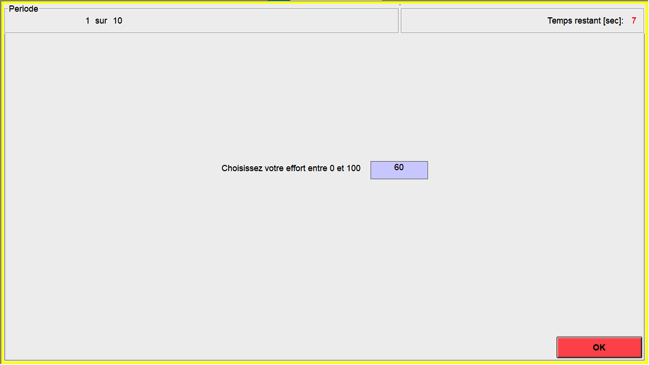
\includegraphics[width = 0.9\textwidth]{05_fig1-annexII.png}

\vspace{0,2cm}
Validez votre choix en cliquant sur «OK». Vous passez à la suite quand
tous les joueurs de votre groupe ont validé leur choix.

\vspace{0,3cm}
\ul{Information sur la somme et la moyenne des efforts des autres
joueurs de votre groupe}

\vspace{0,2cm}
L'écran suivant affiche la somme et la moyenne des efforts choisis par
les trois autres joueurs de votre groupe. L'écran ci-dessous montre un
exemple où la somme des efforts choisis par les trois autres joueurs de
votre groupe est de 140, soit un effort moyen de 140/3~=~46,67 de la
part des trois autres joueurs de votre groupe.

\vspace{0,2cm}
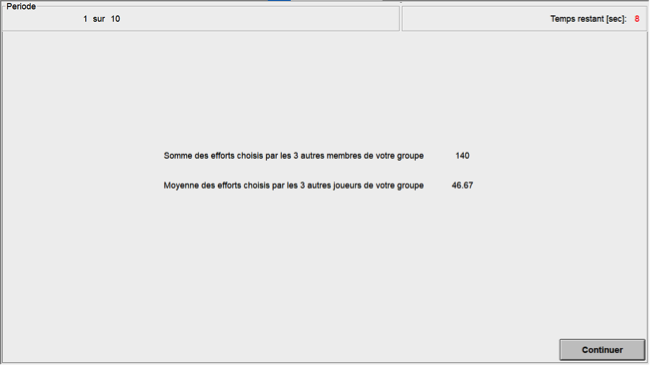
\includegraphics[width = 0.9\textwidth]{05_fig2-annexII.png}
\vspace{0,2cm}

Cliquez sur «Continuer» pour passer à la suite.

\vspace{0,3cm}
\ul{Calcul de votre gain pour la période}

\vspace{0,2cm}
\emph{Votre revenu de production}

\vspace{0,2cm}
Dès que vous-même et les autres joueurs de votre groupe avez validé vos
choix d'effort, l'ordinateur les additionne pour calculer la «Somme des
efforts du groupe». Puis, l'ordinateur tire un nombre entre --~40 et
+~40 au hasard, correspondant à un «Choc aléatoire» qui affecte la
production du groupe. Chaque nombre entre --~40 et +~40 a une même
chance d'être tiré. La «Somme des efforts du groupe» plus ce choc
aléatoire est la «Production totale du groupe», multipliée par 1,5
pour donner le «Revenu total du groupe». Le «Revenu de production»
de chaque joueur vaut un quart du revenu total du groupe.

Par exemple, si vous choisissez un effort de 60 et que la somme des
efforts des autres joueurs de votre groupe est de 140, alors la somme
des efforts du groupe vaut 60~+~140~=~200. Si le choc aléatoire est de
--~40, la production totale du groupe vaut 200~--~40~=~160, le revenu
total du groupe 1,5~×~160~=~240 et votre revenu de production, de même
que celui des trois autres joueurs du groupe, vaut 240/4 =~60.

L'expression de votre revenu de production est~:
\begin{center}
\noindent\fbox{\parbox{\linewidth-2\fboxrule-2\fboxsep}{\centering{Revenu de production \par
=~[1,5~×~(Somme des efforts du groupe~+~Choc aléatoire entre --~40 et
+~40)~/~4]}}}
\end{center}

Votre revenu de production est calculé par l'ordinateur.
\vspace{0,2cm}

\emph{Votre coût de production}

\vspace{0,2cm}
À l'effort que vous choisissez correspond un coût de production, donné
dans le tableau~A ci-dessous.

\newpage

{\centering Tableau A.\par}

{\tabletextsize
\begin{longtable}[]{@{}
  >{\centering\arraybackslash}p{(\columnwidth - 10\tabcolsep) * \real{0.1358}}
  >{\centering\arraybackslash}p{(\columnwidth - 10\tabcolsep) * \real{0.1975}}|
  >{\centering\arraybackslash}p{(\columnwidth - 10\tabcolsep) * \real{0.1358}}
  >{\centering\arraybackslash}p{(\columnwidth - 10\tabcolsep) * \real{0.1975}}|
  >{\centering\arraybackslash}p{(\columnwidth - 10\tabcolsep) * \real{0.1358}}
  >{\centering\arraybackslash}p{(\columnwidth - 10\tabcolsep) * \real{0.1975}}@{}}
\toprule
\begin{minipage}[b]{\linewidth}\centering
Effort choisi
\end{minipage} & \begin{minipage}[b]{\linewidth}\centering
Coût de production
\end{minipage} & \begin{minipage}[b]{\linewidth}\centering
Effort choisi
\end{minipage} & \begin{minipage}[b]{\linewidth}\centering
Coût de production
\end{minipage} & \begin{minipage}[b]{\linewidth}\centering
Effort choisi
\end{minipage} & \begin{minipage}[b]{\linewidth}\centering
Coût de production
\end{minipage} \\
\midrule
0 & 0,00 & 34 & 11,56 & 68 & 46,24 \\
1 & 0,01 & 35 & 12,25 & 69 & 47,61 \\
2 & 0,04 & 36 & 12,96 & 70 & 49,00 \\
3 & 0,09 & 37 & 13,69 & 71 & 50,41 \\
4 & 0,16 & 38 & 14,44 & 72 & 51,84 \\
5 & 0,25 & 39 & 15,21 & 73 & 53,29 \\
6 & 0,36 & 40 & 16,00 & 74 & 54,76 \\
7 & 0,49 & 41 & 16,81 & 75 & 56,25 \\
8 & 0,64 & 42 & 17,64 & 76 & 57,76 \\
9 & 0,81 & 43 & 18,49 & 77 & 59,29 \\
10 & 1,00 & 44 & 19,36 & 78 & 60,84 \\
11 & 1,21 & 45 & 20,25 & 79 & 62,41 \\
12 & 1,44 & 46 & 21,16 & 80 & 64,00 \\
13 & 1,69 & 47 & 22,09 & 81 & 65,61 \\
14 & 1,96 & 48 & 23,04 & 82 & 67,24 \\
15 & 2,25 & 49 & 24,01 & 83 & 68,89 \\
16 & 2,56 & 50 & 25,00 & 84 & 70,56 \\
17 & 2,89 & 51 & 26,01 & 85 & 72,25 \\
18 & 3,24 & 52 & 27,04 & 86 & 73,96 \\
19 & 3,61 & 53 & 28,09 & 87 & 75,69 \\
20 & 4,00 & 54 & 29,16 & 88 & 77,44 \\
21 & 4,41 & 55 & 30,25 & 89 & 79,21 \\
22 & 4,84 & 56 & 31,36 & 90 & 81,00 \\
23 & 5,29 & 57 & 32,49 & 91 & 82,81 \\
24 & 5,76 & 58 & 33,64 & 92 & 84,64 \\
25 & 6,25 & 59 & 34,81 & 93 & 86,49 \\
26 & 6,76 & 60 & 36,00 & 94 & 88,36 \\
27 & 7,29 & 61 & 37,21 & 95 & 90,25 \\
28 & 7,84 & 62 & 38,44 & 96 & 92,16 \\
29 & 8,41 & 63 & 39,69 & 97 & 94,09 \\
30 & 9,00 & 64 & 40,96 & 98 & 96,04 \\
31 & 9,61 & 65 & 42,25 & 99 & 98,01 \\
32 & 10,24 & 66 & 43,56 & 100 & 100,00 \\
33 & 10,89 & 67 & 44,89 & ~ & ~ \\
\bottomrule
\end{longtable}
}

Par exemple, un effort de 10 vous coûte 1~jeton, un effort de 50,
25~jetons, un effort de 100, 100~jetons. Le coût croît plus que
proportionnellement avec l'effort. Ainsi, un effort de 100 coûte plus du
double du coût d'un effort de 50. En résumé~:

\begin{center}
\noindent\fbox{\parbox{\linewidth-2\fboxrule-2\fboxsep}{\centering{Coût de production~=~Coût associé dans le tableau~A à l'effort choisi}}}
\end{center}

Par exemple, un effort de 60 coûte 36~jetons.
\vspace{0,2cm}

\emph{Votre gain pour la période}

\vspace{0,2cm}
Votre gain de production égale votre revenu de production moins votre
coût de production. Votre gain pour la période vaut la somme de ce gain
de production et d'une dotation additionnelle de 10~jetons. En reprenant
les formules précédentes on obtient~:

\begin{center}
\noindent\fbox{\parbox{\linewidth-2\fboxrule-2\fboxsep}{\centering{Gain pour la période
=~Gain de production~+~10
=~Revenu de production~--~Coût de production~+~10
=~[(1,5~×~(Somme des efforts du groupe~+~Choc aléatoire entre --~40 et
+~40)~/~4)
--~Coût de production]~+~10}}}
\end{center}

À noter que votre gain de production est toujours positif ou nul, car si
votre coût de production dépasse votre revenu de production, votre gain
de production est fixé à zéro par l'ordinateur. De ce fait, votre gain
pour la période est toujours supérieur ou égal à 10, du fait de votre
dotation additionnelle de 10~jetons.

Dans l'exemple précédent où vous choisissez un effort de 60 et votre
revenu de production égale aussi 60, votre coût de production vaut 36
d'après le tableau~A, et votre gain de production 60~--~36~=~24~jetons.
En ajoutant 10~jetons additionnels, votre gain pour la période est de
34~jetons.

Votre gain pour la période est calculé par l'ordinateur et restitué à
l'écran~:
\vspace{0,2cm}

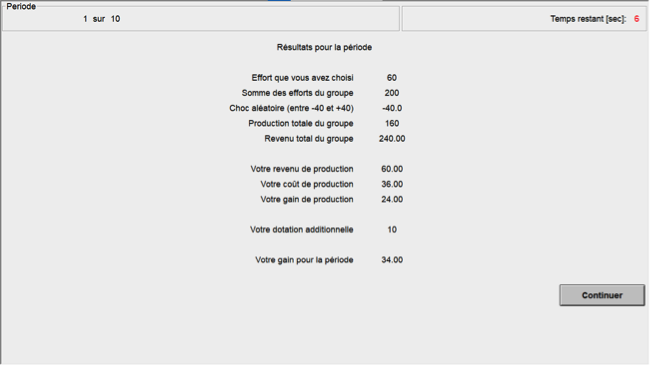
\includegraphics[width = 0.9\textwidth]{05_fig3-annexII.png}

\vspace{0,2cm}
Cliquez sur «Continuer» pour passer à la suite.

\vspace{0,3cm}

\ul{Calcul de votre gain pour l'ensemble de l'expérience}

\vspace{0,2cm}
Votre gain total en jetons pour l'ensemble de l'expérience est égal à la
somme de vos gains pour chacune des 10~périodes de l'expérience. À la
fin du jeu apparaît un écran de synthèse vous indiquant pour les
10~périodes votre gain pour chaque période et le cumul des gains de la
période et des périodes précédentes. Le cumul de vos gains à l'issue de
la dixième période correspond à votre gain total en jetons à l'issue de
l'expérience.

\subsection{Instructions pour le traitement Pression des pairs}

Vous participez à une expérience économique financée par le Centre de
recherches en économie et management de l'Université de Rennes~1. Vous
gagnerez une somme d'argent dont le montant dépendra des décisions que
vous prendrez et des décisions que prendront les autres joueurs.

Il est interdit de communiquer avec d'autres joueurs sous peine
d'exclusion de la session et des gains. Si vous avez des questions,
levez la main. Nous y répondrons en privé.

Durant l'expérience, vos gains sont calculés en jetons. À la fin de
l'expérience, votre gain total en jetons est converti en euros au taux
de 1~euro~=~45~jetons.

À votre gain en jetons converti en euros s'ajoute un forfait de 4~euros.
Vos gains vous sont payés à la fin de l'expérience. Vous seul êtes
informé de la somme que vous avez gagnée.

Au début de l'expérience, les joueurs sont répartis en groupes de
quatre, tirés au hasard. Vous êtes donc avec trois autres joueurs. Ce
groupe correspond à une équipe de production. Vous ne savez pas quels
joueurs font partie de votre groupe. L'expérience consiste en
10~périodes rémunérées. Toutes les périodes sont identiques. Les groupes
restent inchangés durant l'expérience.

Chaque période comprend deux étapes. Ces instructions présentent le
déroulement de la première étape, puis celui de la seconde.
\vspace{0,2cm}

• Première étape

\vspace{0,2cm}
Au début de la première étape apparaît un écran où vous devez choisir un
niveau d'effort, sous la forme d'un nombre compris entre 0 et 100,
représentant votre contribution à la production de votre groupe. Dans
l'exemple d'écran ci-dessous, un effort de 60 est choisi.

\vspace{0,2cm}

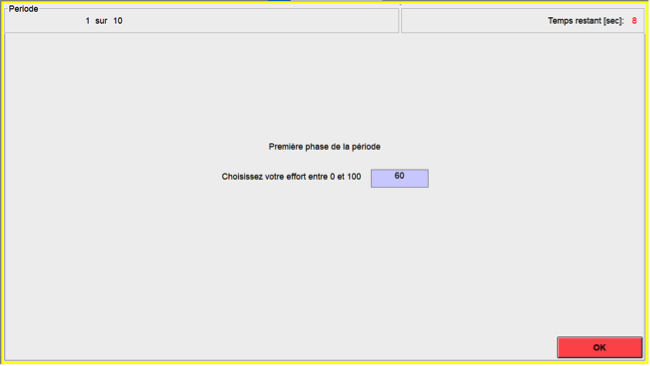
\includegraphics[width = 0.9\textwidth]{05_fig4-annexII.png}

Validez votre choix en cliquant sur «OK». Vous passez à la suite quand
tous les joueurs de votre groupe ont validé leur choix.
\vspace{0,3cm}

\newpage

\ul{Information sur les efforts des autres joueurs}

\vspace{0,2cm}
L'écran suivant affiche les efforts choisis par les autres joueurs de
votre groupe dans un ordre aléatoire qui change à chaque période.
L'écran ci-dessous, montre un exemple où ces trois autres joueurs ont
choisi des efforts de 20, 40 et 80.

\vspace{0,2cm}

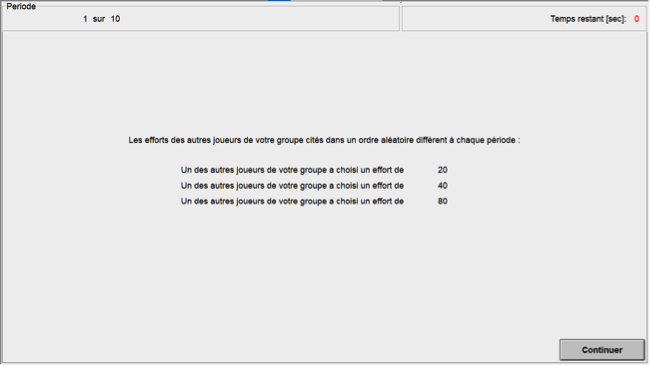
\includegraphics[width = 0.9\textwidth]{05_fig5-annexII.png}

Cliquez sur «Continuer» pour passer à la suite.
\vspace{0,3cm}

\ul{Calcul de votre gain initial après la première étape}

\vspace{0,2cm}

\emph{Votre revenu de production}

\vspace{0,2cm}
Dès que vous-même et les autres joueurs de votre groupe avez validé vos
choix d'effort, l'ordinateur les additionne pour calculer la «Somme des
efforts du groupe». Puis, l'ordinateur tire un nombre entre --~40 et
+~40 au hasard, correspondant à un «Choc aléatoire» qui affecte la
production du groupe. Chaque nombre entre --~40 et +~40 a une même
chance d'être tiré. La «Somme des efforts du groupe» plus ce choc
aléatoire est la «Production totale du groupe», multipliée par 1,5
pour donner le «Revenu total du groupe». Le «Revenu de production»
de chaque joueur vaut un quart du revenu total du groupe.

Par exemple, si vous choisissez un effort de 60 et que la somme des
efforts des autres joueurs de votre groupe est de 140, alors la somme
des efforts du groupe vaut 60~+~140~=~200. Si le choc aléatoire est de
--~40, la production totale du groupe vaut 200~--~40~=~160, le revenu
total du groupe 1,5~×~160~=~240 et votre revenu de production, de même
que celui des trois autres joueurs du groupe, vaut 240/4 =~60.

L'expression de votre revenu de production est~:
\begin{center}
\noindent\fbox{\parbox{\linewidth-2\fboxrule-2\fboxsep}{\centering{Revenu de production \par
=~[1,5~×~(Somme des efforts du groupe~+~Choc aléatoire entre --~40 et
+~40)~/~4]}}}
\end{center}

Votre revenu de production est calculé par l'ordinateur.
\vspace{0,2cm}

\emph{Votre coût de production}

\vspace{0,2cm}
À l'effort que vous choisissez correspond un coût de production, donné
dans le tableau~A ci-dessous.

\vspace{0,2cm}
{\centering Tableau A.\par}

{\tabletextsize
\begin{longtable}[]{@{}
  >{\centering\arraybackslash}p{(\columnwidth - 10\tabcolsep) * \real{0.1358}}
  >{\centering\arraybackslash}p{(\columnwidth - 10\tabcolsep) * \real{0.1975}}|
  >{\centering\arraybackslash}p{(\columnwidth - 10\tabcolsep) * \real{0.1358}}
  >{\centering\arraybackslash}p{(\columnwidth - 10\tabcolsep) * \real{0.1975}}|
  >{\centering\arraybackslash}p{(\columnwidth - 10\tabcolsep) * \real{0.1358}}
  >{\centering\arraybackslash}p{(\columnwidth - 10\tabcolsep) * \real{0.1975}}@{}}
\toprule
\begin{minipage}[b]{\linewidth}\centering
Effort choisi
\end{minipage} & \begin{minipage}[b]{\linewidth}\centering
Coût de production
\end{minipage} & \begin{minipage}[b]{\linewidth}\centering
Effort choisi
\end{minipage} & \begin{minipage}[b]{\linewidth}\centering
Coût de production
\end{minipage} & \begin{minipage}[b]{\linewidth}\centering
Effort choisi
\end{minipage} & \begin{minipage}[b]{\linewidth}\centering
Coût de production
\end{minipage} \\
\midrule
\endhead
\bottomrule
\endlastfoot
0 & 0,00 & 34 & 11,56 & 68 & 46,24 \\
1 & 0,01 & 35 & 12,25 & 69 & 47,61 \\
2 & 0,04 & 36 & 12,96 & 70 & 49,00 \\
3 & 0,09 & 37 & 13,69 & 71 & 50,41 \\
4 & 0,16 & 38 & 14,44 & 72 & 51,84 \\
5 & 0,25 & 39 & 15,21 & 73 & 53,29 \\
6 & 0,36 & 40 & 16,00 & 74 & 54,76 \\
7 & 0,49 & 41 & 16,81 & 75 & 56,25 \\
8 & 0,64 & 42 & 17,64 & 76 & 57,76 \\
9 & 0,81 & 43 & 18,49 & 77 & 59,29 \\
10 & 1,00 & 44 & 19,36 & 78 & 60,84 \\
11 & 1,21 & 45 & 20,25 & 79 & 62,41 \\
12 & 1,44 & 46 & 21,16 & 80 & 64,00 \\
13 & 1,69 & 47 & 22,09 & 81 & 65,61 \\
14 & 1,96 & 48 & 23,04 & 82 & 67,24 \\
15 & 2,25 & 49 & 24,01 & 83 & 68,89 \\
16 & 2,56 & 50 & 25,00 & 84 & 70,56 \\
17 & 2,89 & 51 & 26,01 & 85 & 72,25 \\
18 & 3,24 & 52 & 27,04 & 86 & 73,96 \\
19 & 3,61 & 53 & 28,09 & 87 & 75,69 \\
20 & 4,00 & 54 & 29,16 & 88 & 77,44 \\
21 & 4,41 & 55 & 30,25 & 89 & 79,21 \\
22 & 4,84 & 56 & 31,36 & 90 & 81,00 \\
23 & 5,29 & 57 & 32,49 & 91 & 82,81 \\
24 & 5,76 & 58 & 33,64 & 92 & 84,64 \\
25 & 6,25 & 59 & 34,81 & 93 & 86,49 \\
26 & 6,76 & 60 & 36,00 & 94 & 88,36 \\
27 & 7,29 & 61 & 37,21 & 95 & 90,25 \\
28 & 7,84 & 62 & 38,44 & 96 & 92,16 \\
29 & 8,41 & 63 & 39,69 & 97 & 94,09 \\
30 & 9,00 & 64 & 40,96 & 98 & 96,04 \\
31 & 9,61 & 65 & 42,25 & 99 & 98,01 \\
32 & 10,24 & 66 & 43,56 & 100 & 100,00 \\
33 & 10,89 & 67 & 44,89 & ~ & ~ \\
\end{longtable}
}

Par exemple, un effort de 10 vous coûte 1 jeton, un effort de 50,
25~jetons, un effort de 100, 100~jetons. Le coût croît plus que
proportionnellement avec l'effort. Ainsi, un effort de 100 coûte plus du
double du coût d'un effort de 50. En résumé~:

\begin{center}
\noindent\fbox{\parbox{\linewidth-2\fboxrule-2\fboxsep}{\centering{Coût de production~=~Coût associé dans le tableau~A à l'effort choisi}}}
\end{center}

Par exemple, un effort de 60 coûte 36~jetons.

\vspace{0,2cm}
\emph{Votre gain initial après la première étape}

\vspace{0,2cm}
Votre gain de production égale votre revenu de production moins votre
coût de production. Votre gain initial à l'issue de la première étape
vaut la somme de ce gain de production et d'une dotation additionnelle
de 10~jetons. En reprenant les formules précédentes on obtient~:

\begin{center}
\noindent\fbox{\parbox{\linewidth-2\fboxrule-2\fboxsep}{\centering{Gain pour la période
=~Gain de production~+~10
=~Revenu de production~--~Coût de production~+~10
=~[(1,5~×~(Somme des efforts du groupe~+~Choc aléatoire entre --~40 et
+~40)~/~4)
--~Coût de production]~+~10}}}
\end{center}

À noter que votre gain de production est toujours positif ou nul, car si
votre coût de production dépasse votre revenu de production, votre gain
de production est fixé à zéro par l'ordinateur. De ce fait, votre gain
initial après la première étape est toujours supérieur ou égal à 10, du
fait de votre dotation additionnelle de 10~jetons.

Dans l'exemple précédent où vous choisissez un effort de 60 et votre
revenu de production égale aussi 60, votre coût de production vaut 36
d'après le tableau~A, et votre gain de production 60~--~36~=~24~jetons.
En ajoutant 10~jetons additionnels, votre gain pour la période est de
34~jetons.

Votre gain initial après la première étape est calculé par l'ordinateur
et restitué à l'écran~:

\vspace{0,2cm}

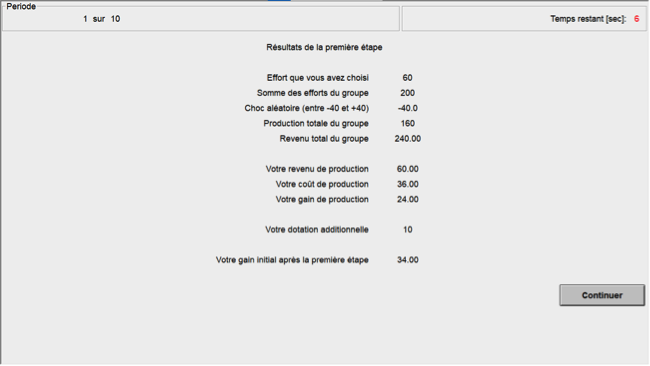
\includegraphics[width = 0.9\textwidth]{05_fig6-annexII.png}

Cliquez sur «Continuer» pour passer à la suite.
\vspace{0,2cm}

•~~Seconde étape

\vspace{0,2cm}
Dans cette seconde étape, vous, comme les autres joueurs du groupe,
pouvez utiliser tout ou partie de vos 10~jetons additionnels pour
réduire les gains des trois autres joueurs de votre groupe en leur
attribuant des points de désapprobation.

Un écran apparaît où vous devez saisir les points de désapprobation que
vous attribuez aux autres joueurs de votre groupe, comme dans l'exemple
ci-dessous~:

\vspace{0,2cm}

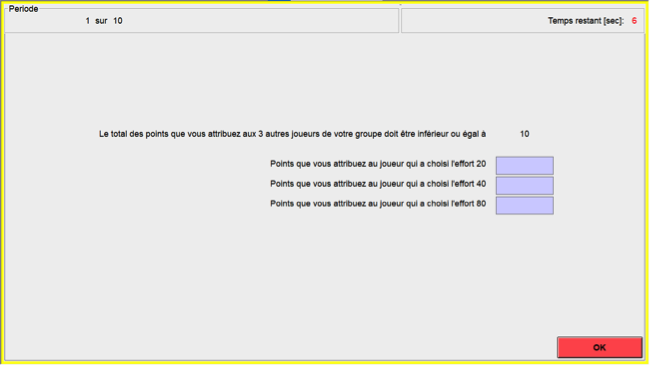
\includegraphics[width = 0.9\textwidth]{05_fig7-annexII.png}

L'ordre d'affichage des efforts des autres joueurs est aléatoire et
varie d'une période à l'autre. C'est donc sur la seule base des efforts
choisis lors de la première étape de cette période que vous décidez des
points que vous leur attribuez. Le nombre total de points attribués aux
trois autres joueurs doit être inférieur ou égal à 10. Validez votre
choix en cliquant sur «OK».
\vspace{0,2cm}

\ul{Gains à l'issue de la seconde étape}

\vspace{0,2cm}
Vous réduisez le gain des autres joueurs du triple du nombre de points
de désapprobation que vous leur attribuez. Si vous attribuez 0~point à
un joueur, vous ne changez pas son gain, si vous lui attribuez 1~point,
vous réduisez son gain de 3~jetons, de 6~jetons si vous lui attribuez
2~points et ainsi de suite.

Attribuer des points aux autres joueurs vous coûte en jetons le total
des points que vous attribuez, ce total ne pouvant dépasser 10~jetons.
Par exemple, attribuer 2~points à chacun des trois autres joueurs vous
coûte 6~jetons. Vous ne pourriez attribuer 5~points à chacun des trois
autres joueurs car cela représenterait 15~points, au-dessus du maximum
de 10.

Votre gain est aussi diminué du triple de nombre total de points de
désapprobation que vous recevez de la part des autres joueurs. Si vous
recevez 0~point, votre gain est inchangé, si vous recevez 1~point, il
baisse de 3~jetons, si vous recevez 2~points, il baisse de 6~jetons,
etc.

Par exemple, si votre gain initial à l'issue de la première étape est de
34~jetons, et si lors de la seconde étape vous attribuez 2~points à
chacun des trois autres joueurs, et si vous recevez des autres joueurs
3~points au total, votre gain final sera de
34~--~3~×~2~--~3~×~3~=~19~jetons.

Plus généralement, votre gain pour la période est calculé de la façon
suivante~:

\begin{center}
\noindent\fbox{\parbox{\linewidth-2\fboxrule-2\fboxsep}{\centering{Gain pour la période
=~Gain initial~--~Nombre total de points attribué~--~3~×~Nombre total de
points reçus}}}
\end{center}

Les points que vous recevez peuvent annuler votre gain mais non le
rendre négatif~: si votre nombre de points reçus dépasse le tiers de
votre gain initial moins le nombre de points que vous attribuez, alors
votre gain pour la période sera considéré comme nul.

Le calcul est fait par l'ordinateur et affiché à l'écran~:

\vspace{0,2cm}

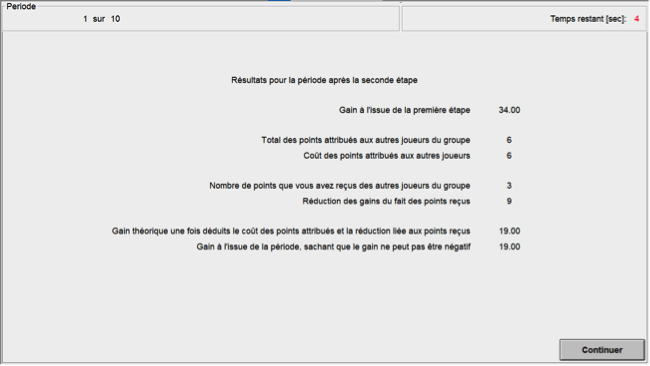
\includegraphics[width = 0.9\textwidth]{05_fig8-annexII.png}

Cliquez sur «Continuer» pour passer à la suite.
\vspace{0,2cm}

\ul{Calcul de votre gain pour l'ensemble de l'expérience}

\vspace{0,2cm}
Votre gain total en jetons pour l'ensemble de l'expérience égale la
somme de vos gains pour chacune des 10~périodes de l'expérience. À la
fin du jeu apparaît un écran de synthèse vous indiquant pour les
10~périodes votre gain pour chaque période et le cumul des gains de la
période et des périodes précédentes. Le cumul de vos gains à l'issue de
la dixième période correspond à votre gain total en jetons à l'issue de
l'expérience.

\subsection{Instructions pour le traitement Objectif d'équipe}

Vous participez à une expérience économique financée par le Centre de
recherches en économie et management de l'Université de Rennes~1. Vous
gagnerez une somme d'argent dont le montant dépendra des décisions que
vous prendrez et des décisions que prendront les autres joueurs.

Il est interdit de communiquer avec d'autres joueurs sous peine
d'exclusion de la session et des gains. Si vous avez des questions,
levez la main. Nous y répondrons en privé.

Durant l'expérience, vos gains sont calculés en jetons. À la fin de
l'expérience, votre gain total en jetons est converti en euros au taux
de 1~euro~=~45~jetons.

À votre gain en jetons converti en euros s'ajoute un forfait de 4~euros.
Vos gains vous sont payés à la fin de l'expérience. Vous seul êtes
informé de la somme que vous avez gagnée.

Au début de l'expérience, les joueurs sont répartis en groupes de
quatre, tirés au hasard. Vous êtes donc avec trois autres joueurs. Ce
groupe correspond à une équipe de production. Vous ne savez pas quels
joueurs font partie de votre groupe. L'expérience consiste en
10~périodes rémunérées. Toutes les périodes sont identiques. Les groupes
restent inchangés durant l'expérience.

Au début de chaque période apparaît un écran où vous devez choisir un
niveau d'effort, sous la forme d'un nombre compris entre 0 et 100,
représentant votre contribution à la production de votre groupe. Dans
l'exemple d'écran ci-dessous, un effort de 60 est choisi.

\vspace{0,2cm}

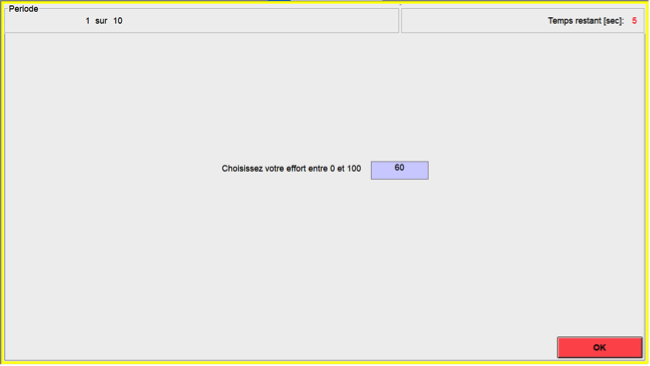
\includegraphics[width = 0.9\textwidth]{05_fig9-annexII.png}

Validez votre choix en cliquant sur «OK». Vous passez à la suite quand
tous les joueurs de votre groupe ont validé leur choix.
\vspace{0,2cm}

\ul{Information sur les efforts des autres joueurs}

\vspace{0,2cm}
L'écran suivant affiche les efforts choisis par les autres joueurs de
votre groupe dans un ordre aléatoire qui change à chaque période.
L'écran ci-dessous montre un exemple où ces trois autres joueurs ont
choisi des efforts de 20, 40 et 80.

\vspace{0,2cm}

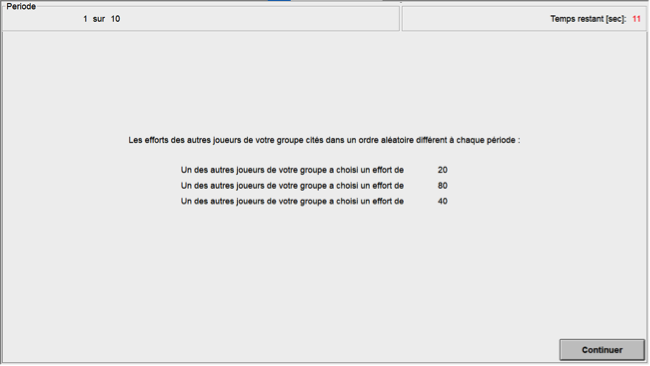
\includegraphics[width = 0.9\textwidth]{05_fig10-annexII.png}

Cliquez sur «Continuer» pour passer à la suite.
\vspace{0,2cm}

\ul{Calcul de votre gain pour la période}

\vspace{0,2cm}
\emph{Votre revenu de production}

\vspace{0,2cm}
Dès que vous-même et les autres joueurs de votre groupe avez validé vos
choix d'effort, l'ordinateur les additionne pour calculer la «Somme des
efforts du groupe». Puis, l'ordinateur tire un nombre entre --~40 et
+~40 au hasard, correspondant à un «Choc aléatoire» qui affecte la
production du groupe. Chaque nombre entre --~40 et +~40 a une même
chance d'être tiré. La «Somme des efforts du groupe» plus ce choc
aléatoire est la «Production totale du groupe», multipliée par 1,5
pour donner le «Revenu total du groupe». Le «Revenu de production»
de chaque joueur vaut un quart du revenu total du groupe.

Si le revenu total du groupe est supérieur ou égal à un seuil fixé à
450~jetons, alors votre revenu de production est égal au quart du revenu
total du groupe. Sinon, votre revenu de production égale un montant
minimal fixe de 7,5~jetons.

Par exemple, si vous choisissez un effort de 60 et les autres joueurs de
votre groupe 20, 40 et 80, la somme des efforts du groupe vaut
60~+~20~+~40~+~80~=~200. Si le choc aléatoire est de --~40, la
production totale du groupe vaut 200~--~40~=~160 et le revenu total du
groupe 1,5~×~160~=~240. Le revenu total du groupe étant inférieur au
seuil de 450, votre revenu de production, de même que celui des trois
autres joueurs du groupe, vaut 7,5~jetons.

Si vous choisissez toujours un effort de 60 mais les autres joueurs de
votre groupe 40, 80 et 100, la somme des efforts du groupe vaut
60~+~40~+~80~+~100~=~280. Si le choc aléatoire est cette fois de +~40,
la production totale du groupe vaut 280~+~40~=~320 et le revenu total du
groupe 1,5~×~320~=~480. Le revenu total du groupe étant supérieur au
seuil de 450, votre revenu de production, de même que celui des trois
autres joueurs du groupe, vaut 480/4~=~120~jetons.

L'expression de votre revenu de production est~:

\begin{center}
\noindent\fbox{\parbox{\linewidth-2\fboxrule-2\fboxsep}{\centering{
    \emph{Si le revenu total du groupe est supérieur ou égal à 450, alors~:}

\vspace{.2cm}

Revenu de production
=~[1,5~×~(Somme des efforts du groupe~+~Choc aléatoire entre --~40 et
+~40)/4]

\vspace{.2cm}

\emph{Si le revenu total du groupe est inférieur à 450, alors~:}

\vspace{.2cm}

Revenu de production~=~7,5
Votre revenu de production est calculé par l'ordinateur.}}}
\end{center}

\emph{Votre coût de production}

\vspace{0,2cm}
À l'effort que vous choisissez correspond un coût de production, donné
dans le tableau~A ci-dessous.

\vspace{0,2cm}
{\centering Tableau A.\par}

{\tabletextsize
\begin{longtable}[]{@{}
  >{\centering\arraybackslash}p{(\columnwidth - 10\tabcolsep) * \real{0.1358}}
  >{\centering\arraybackslash}p{(\columnwidth - 10\tabcolsep) * \real{0.1975}}|
  >{\centering\arraybackslash}p{(\columnwidth - 10\tabcolsep) * \real{0.1358}}
  >{\centering\arraybackslash}p{(\columnwidth - 10\tabcolsep) * \real{0.1975}}|
  >{\centering\arraybackslash}p{(\columnwidth - 10\tabcolsep) * \real{0.1358}}
  >{\centering\arraybackslash}p{(\columnwidth - 10\tabcolsep) * \real{0.1975}}@{}}
\toprule
\begin{minipage}[b]{\linewidth}\centering
Effort choisi
\end{minipage} & \begin{minipage}[b]{\linewidth}\centering
Coût de production
\end{minipage} & \begin{minipage}[b]{\linewidth}\centering
Effort choisi
\end{minipage} & \begin{minipage}[b]{\linewidth}\centering
Coût de production
\end{minipage} & \begin{minipage}[b]{\linewidth}\centering
Effort choisi
\end{minipage} & \begin{minipage}[b]{\linewidth}\centering
Coût de production
\end{minipage} \\
\midrule
\endhead
\bottomrule
\endlastfoot
0 & 0,00 & 34 & 11,56 & 68 & 46,24 \\
1 & 0,01 & 35 & 12,25 & 69 & 47,61 \\
2 & 0,04 & 36 & 12,96 & 70 & 49,00 \\
3 & 0,09 & 37 & 13,69 & 71 & 50,41 \\
4 & 0,16 & 38 & 14,44 & 72 & 51,84 \\
5 & 0,25 & 39 & 15,21 & 73 & 53,29 \\
6 & 0,36 & 40 & 16,00 & 74 & 54,76 \\
7 & 0,49 & 41 & 16,81 & 75 & 56,25 \\
8 & 0,64 & 42 & 17,64 & 76 & 57,76 \\
9 & 0,81 & 43 & 18,49 & 77 & 59,29 \\
10 & 1,00 & 44 & 19,36 & 78 & 60,84 \\
11 & 1,21 & 45 & 20,25 & 79 & 62,41 \\
12 & 1,44 & 46 & 21,16 & 80 & 64,00 \\
13 & 1,69 & 47 & 22,09 & 81 & 65,61 \\
14 & 1,96 & 48 & 23,04 & 82 & 67,24 \\
15 & 2,25 & 49 & 24,01 & 83 & 68,89 \\
16 & 2,56 & 50 & 25,00 & 84 & 70,56 \\
17 & 2,89 & 51 & 26,01 & 85 & 72,25 \\
18 & 3,24 & 52 & 27,04 & 86 & 73,96 \\
19 & 3,61 & 53 & 28,09 & 87 & 75,69 \\
20 & 4,00 & 54 & 29,16 & 88 & 77,44 \\
21 & 4,41 & 55 & 30,25 & 89 & 79,21 \\
22 & 4,84 & 56 & 31,36 & 90 & 81,00 \\
23 & 5,29 & 57 & 32,49 & 91 & 82,81 \\
24 & 5,76 & 58 & 33,64 & 92 & 84,64 \\
25 & 6,25 & 59 & 34,81 & 93 & 86,49 \\
26 & 6,76 & 60 & 36,00 & 94 & 88,36 \\
27 & 7,29 & 61 & 37,21 & 95 & 90,25 \\
28 & 7,84 & 62 & 38,44 & 96 & 92,16 \\
29 & 8,41 & 63 & 39,69 & 97 & 94,09 \\
30 & 9,00 & 64 & 40,96 & 98 & 96,04 \\
31 & 9,61 & 65 & 42,25 & 99 & 98,01 \\
32 & 10,24 & 66 & 43,56 & 100 & 100,00 \\
33 & 10,89 & 67 & 44,89 & ~ & ~ \\
\end{longtable}
}

Par exemple, un effort de 10 vous coûte 1~jeton, un effort de 50,
25~jetons, un effort de 100, 100~jetons. Le coût croît plus que
proportionnellement avec l'effort. Ainsi, un effort de 100 coûte plus du
double du coût d'un effort de 50. En résumé~:

\begin{center}
\noindent\fbox{\parbox{\linewidth-2\fboxrule-2\fboxsep}{\centering{Coût de production~=~Coût associé dans le tableau~A à l'effort choisi}}}
\end{center}

Par exemple, un effort de 60 coûte 36~jetons.
\vspace{.2cm}

\emph{Votre gain pour la période}

\vspace{.2cm}
Votre gain de production égale votre revenu de production moins votre
coût de production. Votre gain pour la période vaut la somme de ce gain
de production et d'une dotation additionnelle de 10~jetons. En reprenant
les formules précédentes on obtient~:

\newpage

\begin{center}
\noindent\fbox{\parbox{\linewidth-2\fboxrule-2\fboxsep}{\centering{
Gain pour la période
=~Gain de production~+~10 \par
=~Revenu de production~--~Coût de production~+~10~=

\vspace{.2cm}
\emph{Si le revenu total du groupe est supérieur ou égal à 450, alors~:}

\vspace{.2cm}
[(1,5~×~(Somme des efforts du groupe~+~Choc aléatoire entre --~40 et
+~40)/4)
--~Coût de production]~+~10

\vspace{.2cm}
\emph{Si le revenu total du groupe est inférieur à 450, alors~:}

\vspace{.2cm}
[7,5~--~Coût de production]~+~10}}}
\end{center}

À noter~: votre gain de production est toujours positif ou nul, car si
votre coût de production dépasse votre revenu de production, votre gain
de production est fixé à zéro par l'ordinateur. De ce fait, votre gain
pour la période est toujours supérieur ou égal à 10, du fait de votre
dotation additionnelle de 10~jetons.

Dans le premier exemple précédent où vous choisissez un effort de 60 et
où le revenu total de votre groupe est égal à 240, en dessous du seuil
de 450, votre revenu de production est fixé à 7,5. Votre coût de
production, égal à 36 d'après le tableau~A, dépasse votre revenu de
production de 7,5. Par suite, l'ordinateur fixe votre gain de production
à 0. En ajoutant 10~jetons additionnels, votre gain pour la période est
de 10~jetons.

Dans le second exemple précédent où vous choisissez toujours un effort
de 60 mais où le revenu total de votre groupe est égal à 480, en dessus
du seuil de 450, votre revenu de production vaut le quart du revenu du
groupe, soit 120. Votre coût de production est égal à 36 d'après le
tableau~A. Par suite, votre gain de production vaut 120~--~36~=~84. En
ajoutant 10~jetons additionnels, votre gain pour la période est de
94~jetons.

Votre gain pour la période est calculé par l'ordinateur et restitué à
l'écran~:

\vspace{0,2cm}

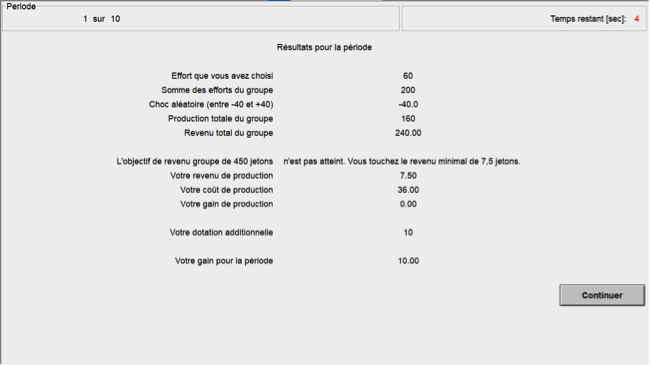
\includegraphics[width = 0.9\textwidth]{05_fig11-annexII.png}

Cliquez sur «Continuer» pour passer à la suite.

\vspace{.2cm}
\ul{Calcul de votre gain pour l'ensemble de l'expérience}

\vspace{.2cm}
Votre gain total en jetons pour l'ensemble de l'expérience égale la
somme de vos gains pour chacune des 10~périodes de l'expérience. À la
fin du jeu apparaît un écran de synthèse vous indiquant pour les
10~périodes votre gain pour chaque période et le cumul des gains de la
période et des périodes précédentes. Le cumul de vos gains à l'issue de
la dixième période correspond à votre gain total en jetons à l'issue de
l'expérience.

\subsection{Instructions pour le traitement Tournois entre équipes}

Vous participez à une expérience économique financée par le Centre de
recherches en économie et management de l'Université de Rennes~1. Vous
gagnerez une somme d'argent dont le montant dépendra des décisions que
vous prendrez et des décisions que prendront les autres joueurs.

Il est interdit de communiquer avec d'autres joueurs sous peine
d'exclusion de la session et des gains. Si vous avez des questions,
levez la main. Nous y répondrons en privé.

Durant l'expérience, vos gains sont calculés en jetons. À la fin de
l'expérience, votre gain total en jetons est converti en euros au taux
de 1~euro~=~45~jetons.

À votre gain en jetons converti en euros s'ajoute un forfait de 4~euros.
Vos gains vous sont payés à la fin de l'expérience. Vous seul êtes
informé de la somme que vous avez gagnée.

Au début de l'expérience, les joueurs sont répartis en groupes de
quatre, tirés au hasard. Vous êtes donc avec trois autres joueurs. Ce
groupe correspond à une équipe de production. Vous ne savez pas quels
joueurs font partie de votre groupe. L'expérience consiste en
10~périodes rémunérées. Toutes les périodes sont identiques. Les groupes
restent inchangés durant l'expérience.

À chaque période, les résultats de votre groupe sont comparés à ceux
d'un groupe concurrent qui reste le même pendant toute l'expérience. Le
groupe vainqueur de cette comparaison reçoit 180~jetons du groupe
vaincu.

Au début de chaque période apparaît un écran où vous devez choisir un
niveau d'effort, sous la forme d'un nombre compris entre 0 et 100,
représentant votre contribution à la production de votre groupe. Dans
l'exemple d'écran ci-dessous, un effort de 60 est choisi.

\vspace{0,2cm}

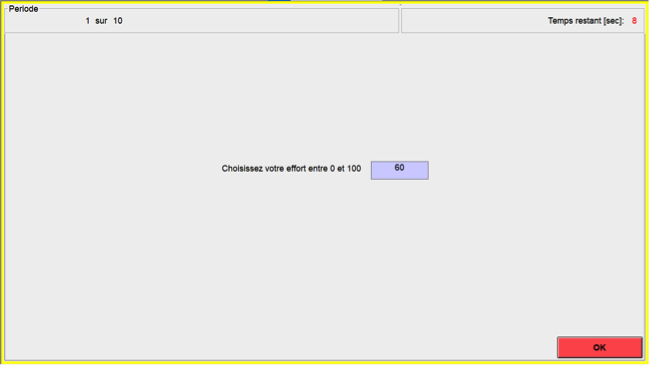
\includegraphics[width = 0.9\textwidth]{05_fig12-annexII.png}

Validez votre choix en cliquant sur «OK». Vous passez à la suite quand
tous les joueurs de votre groupe ont validé leur choix.

\vspace{.2cm}
\ul{Information sur les efforts des autres joueurs}

\vspace{.2cm}
L'écran suivant affiche les efforts choisis par les autres joueurs de
votre groupe dans un ordre aléatoire qui change à chaque période.
L'écran ci-dessous, montre un exemple où ces trois autres joueurs ont
choisi des efforts de 20, 40 et 80.

\vspace{0,2cm}

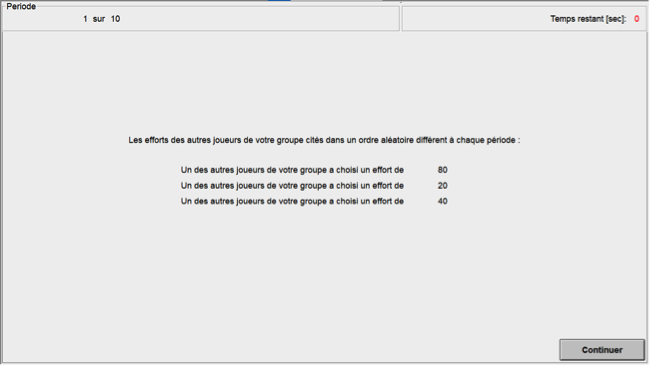
\includegraphics[width = 0.9\textwidth]{05_fig13-annexII.png}

Cliquez sur «Continuer» pour passer à la suite.

\vspace{.2cm}
\ul{Calcul de votre gain pour la période}

\vspace{.2cm}
\emph{Votre revenu de production}

\vspace{.2cm}
Dès que vous-même et les autres joueurs de votre groupe avez validé vos
choix d'effort, l'ordinateur les additionne pour calculer la «Somme des
efforts du groupe». Puis, l'ordinateur tire un nombre entre --~40 et
+~40 au hasard, correspondant à un «Choc aléatoire» qui affecte la
production du groupe. Chaque nombre entre --~40 et +~40 a une même
chance d'être tiré. La «Somme des efforts du groupe» plus ce choc
aléatoire est la «Production totale du groupe», multipliée par 1,5
pour donner le «Revenu total du groupe». Le «Revenu de production»
de chaque joueur vaut un quart du revenu total du groupe.

Le revenu total de votre groupe est comparé à celui du groupe qui est le
concurrent du vôtre pendant toute l'expérience. S'il est supérieur à
celui du concurrent, celui-ci transfère à votre groupe 180~jetons qui
s'ajoutent au revenu total de votre groupe. S'il est inférieur, votre
groupe lui transfère 180~jetons qui se déduisent du revenu total de
votre groupe. En cas d'égalité, aucun transfert n'a lieu.

Le «Revenu de production» de chaque joueur vaut un quart du revenu
total du groupe après transfert.

Par exemple, si vous choisissez un effort de 60 et les autres joueurs de
votre groupe 20, 40 et 80, la somme des efforts du groupe vaut
60~+~20~+~40~+~80~=~200. Si le choc aléatoire est de --~40, la
production totale du groupe vaut 200~--~40~=~160 et le revenu total du
groupe 1,5~×~160~=~240.

Si, dans cet exemple, le groupe concurrent a un revenu total supérieur à
240, donc supérieur au vôtre, votre groupe lui transfère 180~jetons qui
se déduisent du revenu total de votre groupe~: il ne reste donc que
240~--~180~=~60~jetons à répartir entre les quatre joueurs de votre
groupe. D'où pour chacun un revenu individuel de production de
60/4~=~15~jetons.

Si, dans cet exemple, le groupe concurrent a un revenu total inférieur à
240, donc inférieur au vôtre, il transfère à votre groupe 180~jetons qui
s'ajoutent au revenu total de votre groupe~: il y a donc
240~+~180~=~420~jetons à répartir entre les quatre joueurs de votre
groupe. D'où pour chacun un revenu individuel de production de
420/4~=~105~jetons.

L'expression générale de votre revenu de production est la suivante~:

\begin{center}
\noindent\fbox{\parbox{\linewidth-2\fboxrule-2\fboxsep}{\centering{Revenu de production =~[(1,5~×~(Somme des efforts du groupe~+~Choc aléatoire de production
entre --~40 et +~40)~+~180)/4]

\emph{si le revenu total de votre groupe est supérieur à celui du groupe
concurrent}

\vspace{.3cm}
Revenu de production
=~[(1,5~×~(Somme des efforts du groupe~+~Choc aléatoire de production
entre --~40 et +~40)~--~180)/4]

\emph{si le revenu total de votre groupe est inférieur à celui du groupe
concurrent}}}}
\end{center}


\vspace{.2cm}
Votre revenu de production est calculé par l'ordinateur.

\vspace{.3cm}
\emph{Votre coût de production}

\vspace{.2cm}
À l'effort que vous choisissez correspond un coût de production, donné
dans le tableau~A ci-dessous.

\vspace{0,2cm}
{\centering Tableau A.\par}

{\tabletextsize
\begin{longtable}[]{@{}
  >{\centering\arraybackslash}p{(\columnwidth - 10\tabcolsep) * \real{0.1358}}
  >{\centering\arraybackslash}p{(\columnwidth - 10\tabcolsep) * \real{0.1975}}|
  >{\centering\arraybackslash}p{(\columnwidth - 10\tabcolsep) * \real{0.1358}}
  >{\centering\arraybackslash}p{(\columnwidth - 10\tabcolsep) * \real{0.1975}}|
  >{\centering\arraybackslash}p{(\columnwidth - 10\tabcolsep) * \real{0.1358}}
  >{\centering\arraybackslash}p{(\columnwidth - 10\tabcolsep) * \real{0.1975}}@{}}
\toprule
\begin{minipage}[b]{\linewidth}\centering
Effort choisi
\end{minipage} & \begin{minipage}[b]{\linewidth}\centering
Coût de production
\end{minipage} & \begin{minipage}[b]{\linewidth}\centering
Effort choisi
\end{minipage} & \begin{minipage}[b]{\linewidth}\centering
Coût de production
\end{minipage} & \begin{minipage}[b]{\linewidth}\centering
Effort choisi
\end{minipage} & \begin{minipage}[b]{\linewidth}\centering
Coût de production
\end{minipage} \\
\midrule
\endhead
\bottomrule
\endlastfoot
0 & 0,00 & 34 & 11,56 & 68 & 46,24 \\
1 & 0,01 & 35 & 12,25 & 69 & 47,61 \\
2 & 0,04 & 36 & 12,96 & 70 & 49,00 \\
3 & 0,09 & 37 & 13,69 & 71 & 50,41 \\
4 & 0,16 & 38 & 14,44 & 72 & 51,84 \\
5 & 0,25 & 39 & 15,21 & 73 & 53,29 \\
6 & 0,36 & 40 & 16,00 & 74 & 54,76 \\
7 & 0,49 & 41 & 16,81 & 75 & 56,25 \\
8 & 0,64 & 42 & 17,64 & 76 & 57,76 \\
9 & 0,81 & 43 & 18,49 & 77 & 59,29 \\
10 & 1,00 & 44 & 19,36 & 78 & 60,84 \\
11 & 1,21 & 45 & 20,25 & 79 & 62,41 \\
12 & 1,44 & 46 & 21,16 & 80 & 64,00 \\
13 & 1,69 & 47 & 22,09 & 81 & 65,61 \\
14 & 1,96 & 48 & 23,04 & 82 & 67,24 \\
15 & 2,25 & 49 & 24,01 & 83 & 68,89 \\
16 & 2,56 & 50 & 25,00 & 84 & 70,56 \\
17 & 2,89 & 51 & 26,01 & 85 & 72,25 \\
18 & 3,24 & 52 & 27,04 & 86 & 73,96 \\
19 & 3,61 & 53 & 28,09 & 87 & 75,69 \\
20 & 4,00 & 54 & 29,16 & 88 & 77,44 \\
21 & 4,41 & 55 & 30,25 & 89 & 79,21 \\
22 & 4,84 & 56 & 31,36 & 90 & 81,00 \\
23 & 5,29 & 57 & 32,49 & 91 & 82,81 \\
24 & 5,76 & 58 & 33,64 & 92 & 84,64 \\
25 & 6,25 & 59 & 34,81 & 93 & 86,49 \\
26 & 6,76 & 60 & 36,00 & 94 & 88,36 \\
27 & 7,29 & 61 & 37,21 & 95 & 90,25 \\
28 & 7,84 & 62 & 38,44 & 96 & 92,16 \\
29 & 8,41 & 63 & 39,69 & 97 & 94,09 \\
30 & 9,00 & 64 & 40,96 & 98 & 96,04 \\
31 & 9,61 & 65 & 42,25 & 99 & 98,01 \\
32 & 10,24 & 66 & 43,56 & 100 & 100,00 \\
33 & 10,89 & 67 & 44,89 & ~ & ~ \\
\end{longtable}
}

Par exemple, un effort de 10 vous coûte 1~jeton, un effort de 50,
25~jetons, un effort de 100, 100~jetons. Le coût croît plus que
proportionnellement avec l'effort. Ainsi, un effort de 100 coûte plus du
double du coût d'un effort de 50. En résumé~:

\begin{center}
\noindent\fbox{\parbox{\linewidth-2\fboxrule-2\fboxsep}{\centering{
    Coût de production~=~Coût associé dans le tableau~A à l'effort choisi}}}
\end{center}

Par exemple, un effort de 60 coûte 36~jetons.

\vspace{.2cm}
\emph{Votre gain pour la période}

\vspace{.2cm}
Votre gain de production égale votre revenu de production moins votre
coût de production. Votre gain pour la période vaut la somme de ce gain
de production et d'une dotation additionnelle de 10~jetons. En reprenant
les formules précédentes on obtient~:

\begin{center}
\noindent\fbox{\parbox{\linewidth-2\fboxrule-2\fboxsep}{\centering{
Gain pour la période
=~Gain de production~+~10 \par
=~Revenu de production~--~Coût de production~+~10 \par
=~[(1,5~×~(Somme des efforts du groupe~+~Choc aléatoire de production \par
entre --~40 et +~40)~+~180)/4] --~Coût de production)~+~10

\emph{si le revenu total de votre groupe est supérieur à celui du groupe
concurrent}

\vspace{.2cm}
=~[(1,5~×~(Somme des efforts du groupe~+~Choc aléatoire de production \par
entre --~40 et +~40)~--~180)/4]~--~Coût de production)~+~10

\emph{si le revenu total de votre groupe est inférieur à celui du groupe
concurrent}}}}
\end{center}

À noter~: votre gain de production est toujours positif ou nul, car si
votre coût de production dépasse votre revenu de production, votre gain
de production est fixé à zéro par l'ordinateur. De ce fait, votre gain
pour la période est toujours supérieur ou égal à 10, du fait de votre
dotation additionnelle de 10~jetons.

Dans le premier exemple précédent, où vous choisissez un effort de 60 et
où le revenu total de votre groupe de 240 est inférieur à celui du
groupe concurrent, votre revenu de production est réduit à
(240~--~180)/4~=~60/4~=~15~jetons du fait du transfert de 180~jetons au
groupe concurrent. Votre coût de production résultant de votre effort de
60 vaut 36 d'après le tableau~A. Comme votre revenu de production de 15
est inférieur à votre coût de production de 36, votre gain de production
est ramené à 0. Avec 10~jetons additionnels, votre gain pour la période
est de 10~jetons.

Dans le second exemple précédent, où vous choisissez un effort de 60 et
où le revenu total de votre groupe de 240 est supérieur à celui du
groupe concurrent, votre revenu de production est porté à
(240~+~180)/4~=~420/4~=~105~jetons grâce au transfert de 180~jetons du
groupe concurrent. Votre coût de production résultant de votre effort de
60 vaut 36 d'après le tableau~A~: votre gain de production est égal à la
différence entre votre revenu de production de 105 et votre coût de
production de 36, soit 69. Avec 10~jetons additionnels, votre gain pour
la période est de 79~jetons.

% \newpage

Votre gain pour la période est calculé par l'ordinateur et restitué à
l'écran~:

\vspace{.3cm}

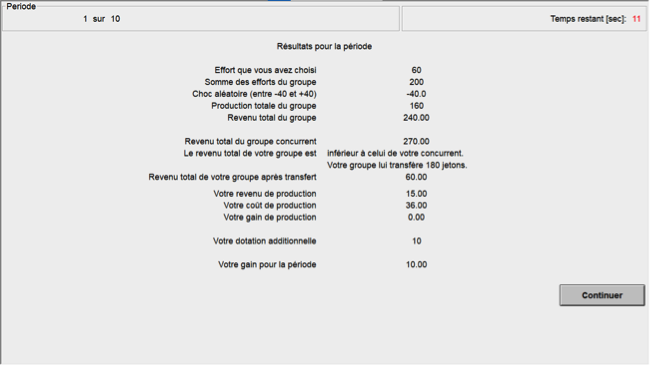
\includegraphics[width = 0.9\textwidth]{05_fig14-annexII.png}

Cliquez sur «Continuer» pour passer à la suite.

\vspace{.3cm}
\ul{Calcul de votre gain pour l'ensemble de l'expérience}

\vspace{.2cm}
Votre gain total en jetons pour l'ensemble de l'expérience égale la
somme de vos gains pour chacune des 10~périodes de l'expérience. À la
fin du jeu apparaît un écran de synthèse vous indiquant pour les
10~périodes votre gain pour chaque période et le cumul des gains de la
période et des périodes précédentes. Le cumul de vos gains à l'issue de
la dixième période correspond à votre gain total en jetons à l'issue de
l'expérience.

\section{Questionnaire post-expérience --\\ pour tous les traitements}
\label{Annexe:Questionnaire}

\subsection{Questions concernant les caractéristiques sociodémographiques des participants}

--~\emph{Quel âge avez-vous~?}

--~\emph{Quel est votre genre~?} Masculin / Féminin

--~\emph{Le français est-il votre langue maternelle~?} Oui / Non

--~\emph{Êtes-vous un(e) étudiant(e) étranger(ère)~?} Oui / Non / Je ne suis
pas étudiant(e)/Je préfère ne pas répondre

--~\emph{Quel est votre niveau d'étude~?} Licence~1 / Licence~2 /
Licence 3 / Master 1 / Master 2 / \textgreater Master / Autres

--~\emph{Quelle est votre discipline actuelle~?} Sciences économiques /
Administration sociale et économique / Droit / Gestion / Sciences
politiques / Littérature / Chimie / Physique / Médecine / Autres

--~\emph{Quelle université ou école fréquentez-vous~?} Université /
École de commerce / École d'ingénieur / Autres

--~\emph{À combien de session(s) expérimentale(s) rémunérée(s) avez-vous
participé avant cette session~?} Jamais / Une / Deux ou plus


\subsection{Questions concernant le jeu (questions ouvertes)}

\emph{--~Les règles du jeu vous ont-elles paru claires~?}

\emph{--~Quelle a été votre stratégie de jeu~?}

\emph{--~À votre avis, quel est le but de cette expérience~?}

\section{Éléments statistiques supplémentaires}
\label{Annexe:Éléments stats}

Les éléments statistiques supplémentaires concernent les points
suivants~:

1.~Significativité des différences de caractéristiques démographiques
entre participants aux différents traitements.

2.~Analyse statistique du comportement de sanction dans le traitement
avec Pression des pairs.

3.~Évolution de la dispersion des efforts au sein des équipes, dans le
traitement avec Objectif d'équipe.

4.~Significativité des différences de profits des firmes et du revenu
total entre traitements.

5.~Évolution de la composition de la richesse totale au fil du temps par
traitement.


\subsection{Significativité des différences de caractéristiques
démographiques entre participants aux différents traitements}
\label{Annexe:Significativité différences}

%Tableau A1

{\centering \textsc{Tableau A1} -- \emph{Résultats des tests sur les différences sociodémographiques\\ entre traitements}\par}

\begin{table}[h!]
% \caption{Résultats des tests sur les différences sociodémographiques\\ entre traitements}
\label{tab_A1}
\centering
\begin{tabular}{p{4.2cm}D{1cm}D{1.2cm}D{1.670cm}D{1cm}}
\toprule
    & Genre* & Participation* & Sciences économiques* & Âge\textsuperscript{≠} \tabularnewline
\midrule
Baseline \emph{vs} Pression pairs & 0,371 & 1,000 & 0,666 & 0,5905 \tabularnewline
Baseline \emph{vs} Objectif d'équipe & 0,770 & 0,048 & 0,416 & 0,8892 \tabularnewline
Baseline \emph{vs} Tournois entre équipes & 0,803 & 0,007 & 0,196 & 0,8978 \tabularnewline
Pression pairs \emph{vs} Objectif d'équipe & 0,760 & 0,137 & 1,000 & 0,4223 \tabularnewline
Pression pairs \emph{vs} Tournois entre équipes & 0,439 & 0,023 & 0,759 & 0,3103 \tabularnewline
Objectif d'équipe \emph{vs} Tournois entre équipes & 0,803 & 0,794 & 1,000 & 0,9416 \tabularnewline
\bottomrule
\end{tabular}
\notedetableau{*~Test exact de Fisher~; χ\textsuperscript{2} tests
donnent des résultats qualitativement similaires.
\textsuperscript{≠}~\emph{t}-test.}
\end{table}


\subsection{Analyse statistique du comportement de sanction\\ dans le
traitement avec Pression des pairs}
\label{Annexe:Analyse statist comport}

\vspace{.2cm}
Dans un premier temps, nous présentons les statistiques sur l'évolution
de la proportion de punisseurs au fil du temps. Ensuite, nous présentons
une analyse comparée des caractéristiques et du comportement des
punisseurs ultimes (c'est-à-dire ceux qui punissent lors de la dernière
période du jeu) et de ceux qui ne sont pas punisseurs ultimes.

\begin{figure}[h]
    \centering
    \caption{Évolution de la proportion de punisseurs au fil du temps}
    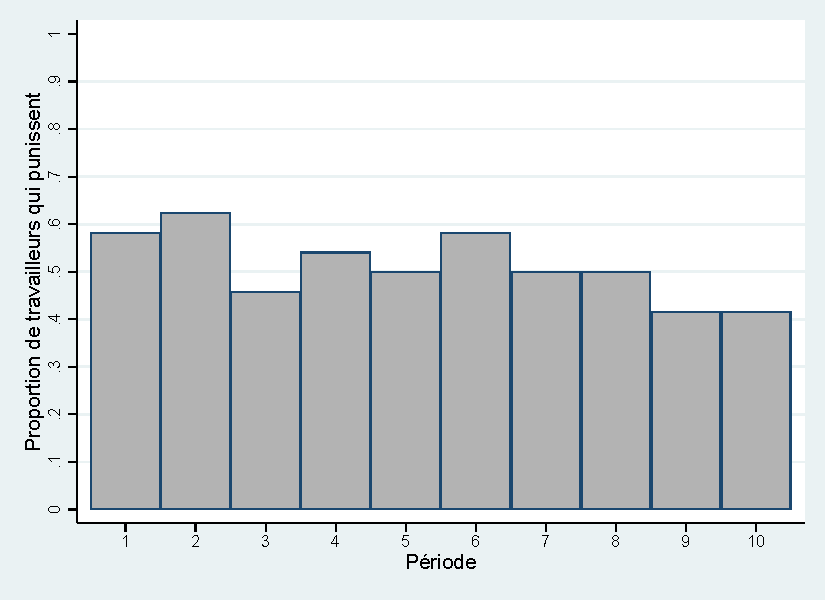
\includegraphics[height=6cm]{05_graphA1.pdf}
\end{figure}

La figure~A1 présente l'évolution de la proportion de punisseurs au
cours du temps. Il indique que cette proportion est plutôt stable. La
différence de proportion de punisseurs entre les cinq premières périodes
et les cinq dernières n'est pas significative selon un test de Fisher
non paramétrique (\emph{p}~=~0,439).

Parmi les 24~participants ayant joué le traitement Pression des pairs,
10 punissent lors de la période~10. Nous les appelons punisseurs
ultimes. Il est intéressant de mieux comprendre ces punisseurs ultimes
puisqu'ils ne punissent pas pour des raisons stratégiques, c'est-à-dire
en vue de favoriser une coopération future. Une explication possible est
que ces punisseurs ultimes sont motivés par des raisons non
stratégiques, telles que la réciprocité, la vengeance aveugle
(\textcite{Nikiforakis2004}~; \textcite{DenantBoemontMascletNoussair2007}), voire une pure volonté de nuire aux autres (\emph{pure
nastiness}) ou un désir de domination (\textcite{Zizzo2003}~; \textcite{CinyabugumaPagePutterman2004}, \textcite{CinyabugumaPagePutterman2006}). D'autres travaux antérieurs ont étudié la relation entre les émotions et la volonté de punir, et en
particulier comment la colère accompagne l'application d'une punition
coûteuse dans les interactions bilatérales (\textcite{BosmanVanWinden2002}~; \textcite{BenShakharBornsteinHopfensitzVanWinden2007}) ou dans des jeux de bien
public avec sanction (voir par exemple \textcite{JoffilyMascletNoussairVilleval2014}~; \textcite{DickinsonMasclet2015}). Ces études mesurent les
émotions au moyen d'auto-évaluations ou en utilisant des mesures
électrophysiologiques de l'excitation émotionnelle.

Les tableaux~A2 et A3 présentent des statistiques descriptives
concernant les efforts, les points attribués et les données
démographiques pour les 10~punisseurs ultimes et les autres punisseurs,
respectivement.

\vspace{0.2cm}
{\centering \textsc{Tableau A2} -- \emph{Statistiques descriptives concernant les punisseurs ultimes}\par}
\begin{table}[h!]
% \caption{Statistiques descriptives concernant les punisseurs ultimes}
\label{tab_A2}
\centering
\begin{tabular}{p{2.8cm}D{1.2cm}D{1.2cm}D{1.2cm}D{1cm}D{1cm}}
\toprule
& Observations & Moyenne & Écart type & Min & Max \tabularnewline
\midrule
Effort & 100 & 58,13 & 20,69 & 10 & 100 \tabularnewline
Points attribués & 100 & 2,1 & 2,35 & 0 & 9 \tabularnewline
Genre & 10 & 0,1 & 0,32 & 0 & 1 \tabularnewline
Participation précédente & 10 & 0 & 0 & 0 & 0 \tabularnewline
Sciences économiques & 10 & 0,1 & 0,32 & 0 & 1 \tabularnewline
Âge & 10 & 21,1 & 1,73 & 18 & 24 \tabularnewline
\bottomrule
\end{tabular}
\end{table}

\vspace{0.2cm}
{\centering \textsc{Tableau A3} -- \emph{Statistiques descriptives concernant les non-punisseurs ultimes}\par}
\begin{table}[h!]
% \caption{Statistiques descriptives concernant les non-punisseurs ultimes}
\label{tab_A3}
\centering
\begin{tabular}{p{2.8cm}D{1.2cm}D{1.2cm}D{1.2cm}D{1cm}D{1cm}}
\toprule
& Observations & Moyenne & Écart type & Min & Max \tabularnewline
\midrule
Effort & 140 & 53,96 & 26,02 & 0 & 100 \tabularnewline
Points attribués & 140 & 1,62 & 2,47 & 0 & 10 \tabularnewline
Genre & 14 & 0,43 & 0,51 & 0 & 1 \tabularnewline
Participation précédente & 14 & 0,14 & 0,36 & 0 & 1 \tabularnewline
Sciences économiques & 14 & 0,21 & 0,43 & 0 & 1 \tabularnewline
Âge & 14 & 20,86 & 2,68 & 18 & 27 \tabularnewline
\bottomrule
\end{tabular}
\end{table}

Le tableau~A4 présente les résultats de tests statistiques afin de
vérifier s'il existe ou pas des différences d'effort, de points
attribués et de caractéristiques démographiques entre les punisseurs
ultimes et les autres. Ce tableau indique l'absence de différences
significatives entre ces différents punisseurs. Autrement dit, il semble
que les punisseurs ultimes ne sont pas significativement différents des
autres punisseurs.

\vspace{0.2cm}
{\centering \textsc{Tableau A4} -- \emph{Significativité des différences entre punisseurs ultimes et les autres}\par}
\begin{table}[h!]
% \caption{Significativité des différences entre punisseurs ultimes et
% les autres}
\label{tab_A4}
\centering
\begin{tabular}{m{2.2cm}D{0.5cm}D{1.1cm}D{0.75cm}D{1.4cm}D{1.6cm}D{0.6cm}}
\toprule
& Effort & Points attribués\textsuperscript{≠} & Genre* & Participation précédente* & Sciences économiques* & Âge\textsuperscript{≠} \tabularnewline
\midrule
Punisseurs ultimes \emph{vs} Autres & 0,18 & 0,13 & 0,17 & 0,49 & 0,44 & 0,80 \tabularnewline
\bottomrule
\end{tabular}
\notedetableau{*~Test exact de Fisher~; \textsuperscript{≠}~\emph{t}-test.}
\end{table}

\begin{figure}[h]
    \centering
    \caption{Évolution du nombre moyen de points attribués par les punisseurs ultimes}
    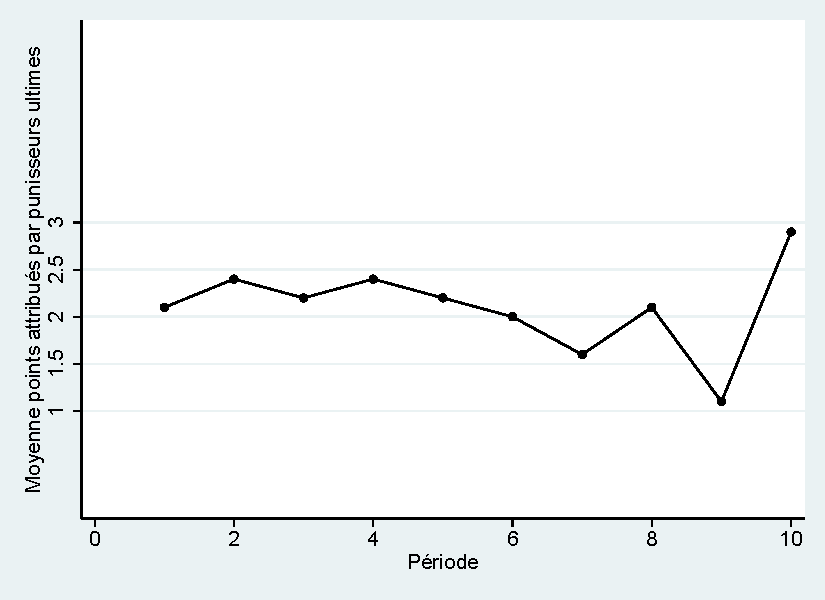
\includegraphics[height=6cm]{05_graphA2.pdf}
\end{figure}

La figure~A2 montre l'évolution du nombre moyen de points de sanction
attribués par les punisseurs ultimes. On note d'abord une légère baisse
du niveau moyen de punition, puis une forte hausse lors de la période
finale, qui pourrait être interprétée comme un effet de fin de partie.
Les punisseurs ultimes attribuent en moyenne 2,9~points lors de la
période~10.

\begin{figure}[h]
    \centering
    \caption{Évolution du nombre moyen de points attribués par les non-punisseurs ultimes}
    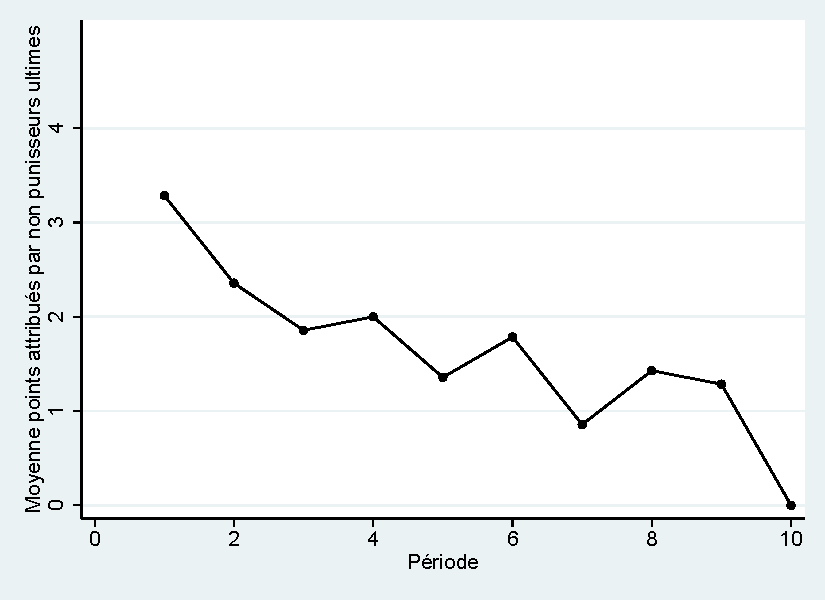
\includegraphics[height=6cm]{05_graphA3.pdf}
\end{figure}

La figure~A3 présente l'évolution du nombre moyen de points attribués
par ceux qui ne sont pas punisseurs ultimes. Elle fait apparaître une
tendance négative.

\newpage

\subsection{Évolution de la dispersion des efforts au sein des équipes, dans
le traitement avec Objectif d'équipe}
\label{Annexe:Évolution dispersion des efforts}

L'analyse de la dispersion de l'effort et de son évolution dans le temps
est présentée graphiquement, à l'aide de boîtes à moustaches. Cette
analyse est réalisée séparément pour les équipes qui parviennent à
atteindre l'objectif et pour les équipes qui ne parviennent pas à
atteindre cet objectif. À noter que les équipes qui réussissent ou
échouent à atteindre l'objectif peuvent changer d'une période à l'autre.

La figure~A4 montre l'évolution de la dispersion des efforts des
travailleurs des équipes qui atteignent l'objectif fixé par
l'entreprise.

\begin{figure}[h!]
    \centering
    \caption{Évolution de la dispersion des efforts, dans l'ensemble des équipes qui atteignent l'objectif}
    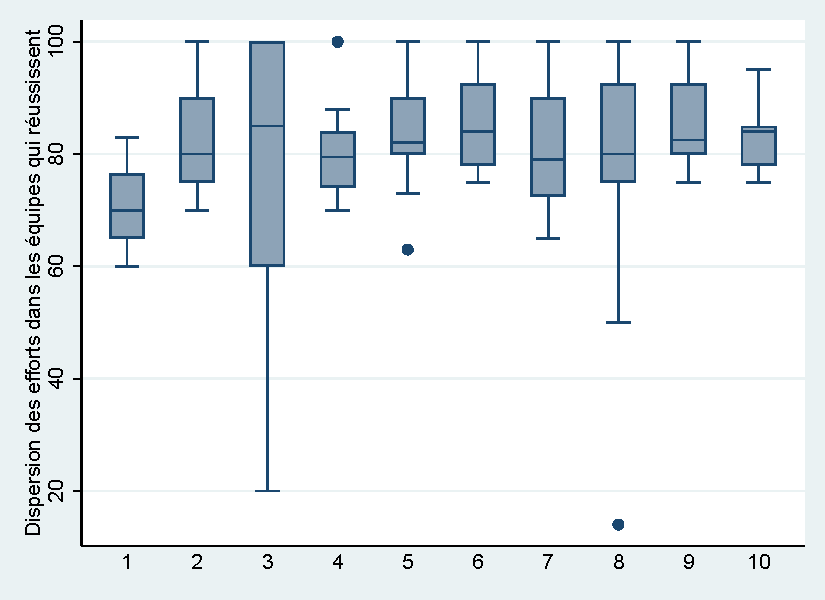
\includegraphics[height=6cm]{05_graphA4.pdf}
\notedetableau{Les boîtes à moustaches indiquent les quartiles. La ligne
au milieu de chaque case correspond à la médiane. La limite inférieure
de chaque case correspond au premier quartile et la limite supérieure au
troisième quartile. La moustache inférieure est égale au maximum entre
le minimum de la distribution et le premier quartile moins 1,5~fois la
différence entre le troisième et le premier quartile. La moustache la
plus élevée est égale au minimum entre le maximum de la distribution et
le troisième quartile plus 1,5~fois la différence entre le troisième et
le premier quartile. Les points correspondent aux valeurs extrêmes, soit
sous la moustache inférieure, soit au-dessus de la moustache supérieure.
Ils correspondent aux valeurs aberrantes, c'est-à-dire des points de
données qui se situent à une distance significative des autres valeurs
de l'échantillon.}
\end{figure}

La figure~A4 ne montre aucune tendance claire de réduction de la
dispersion des efforts parmi les travailleurs des équipes qui atteignent
l'objectif.
La figure~A5 présente plus en détail l'évolution de la dispersion des
efforts entre les travailleurs au sein de chaque équipe lorsque celle-ci
atteint l'objectif.

\begin{figure}[h]
    \centering
    \caption{Évolution de la dispersion des efforts, au sein de chacune des équipes lorsqu'elles atteignent l'objectif}
    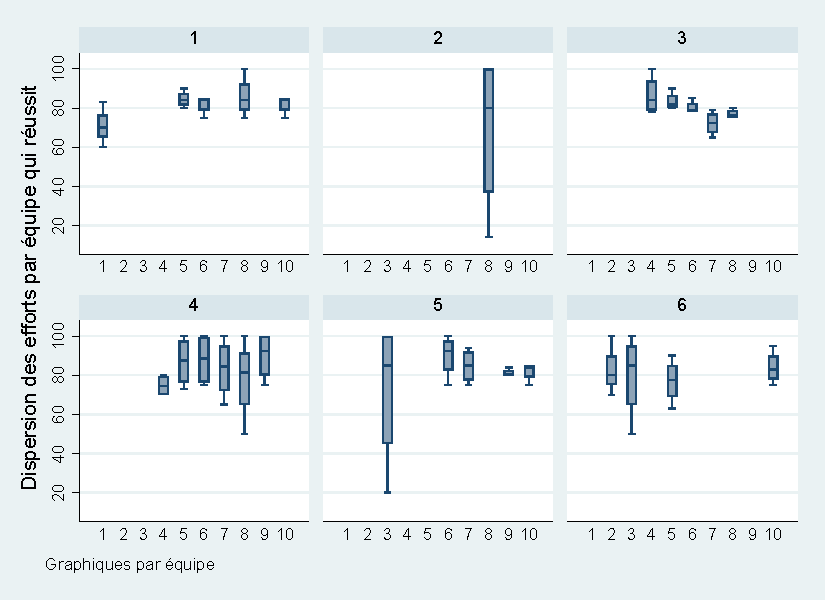
\includegraphics[height=6cm]{05_graphA5.pdf}
\end{figure}

La figure~A5 ne présente pas non plus de tendance claire à la
réduction de la dispersion des efforts des travailleurs, au sein des
équipes qui atteignent l'objectif.
La figure~A6 montre l'évolution de la dispersion des efforts entre
les travailleurs de toutes les équipes qui n'atteignent pas l'objectif.
Elle indique que le niveau de dispersion des efforts est relativement
élevé dans les équipes qui échouent à atteindre l'objectif contrairement
aux équipes qui réussissent (figure~A4). À noter que les équipes qui
échouent peuvent manquer d'atteindre l'objectif malgré des efforts
relativement élevés de leurs membres, en raison d'un choc de production
aléatoire négatif. La figure ne montre pas de réduction de la
dispersion des efforts ni d'indice de découragement des travailleurs.

\begin{figure}[h]
    \centering
    \caption{Évolution de la dispersion des efforts, dans l'ensemble des équipes qui n'atteignent pas l'objectif}
    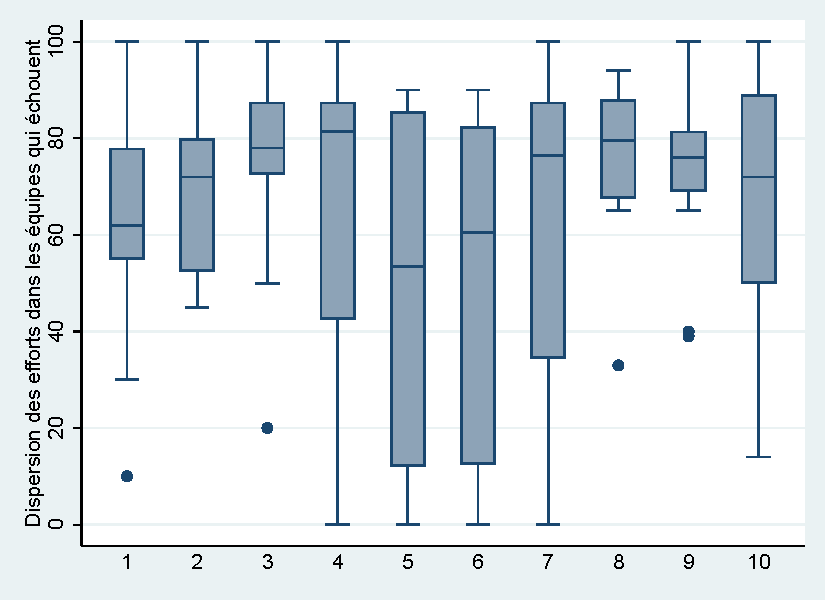
\includegraphics[height=6cm]{05_graphA6.pdf}
\notedetableau{Les boîtes à moustaches indiquent les quartiles. La ligne
au milieu de chaque case correspond à la médiane. La limite inférieure
de chaque case correspond au premier quartile et la limite supérieure au
troisième quartile. La moustache inférieure est égale au maximum entre
le minimum de la distribution et le premier quartile moins 1,5~fois la
différence entre le troisième et le premier quartile. La moustache la
plus élevée est égale au minimum entre le maximum de la distribution et
le troisième quartile plus 1,5~fois la différence entre le troisième et
le premier quartile. Les points correspondent aux valeurs extrêmes, soit
sous la moustache inférieure, soit au-dessus de la moustache supérieure.
Ils correspondent aux valeurs aberrantes, c'est-à-dire des points de
données qui se situent à une distance significative des autres valeurs
de l'échantillon.}
\end{figure}

La figure~A7 analyse plus en détail l'évolution de la dispersion des
efforts entre les travailleurs au sein de chaque équipe dès lors
qu'elles n'atteignent pas l'objectif. Elle indique également davantage de
dispersion que dans le cas des équipes qui atteignent l'objectif
(figure~A5). Cette figure ne montre aucune tendance à la réduction de
la dispersion des efforts dans les équipes qui échouent à atteindre
l'objectif.

\begin{figure}[h]
    \centering
    \caption{Évolution de la dispersion des efforts, au sein de chacune des équipes lorsqu'elles n'atteignent pas l'objectif}
    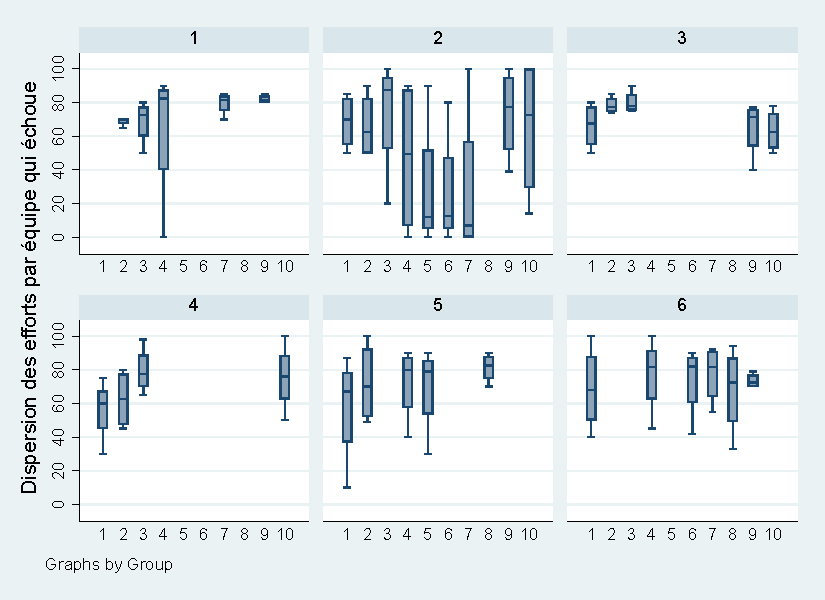
\includegraphics[height=6cm]{05_graphA7.pdf}
\end{figure}

\subsection{Significativité des différences de profits des firmes\\ et du revenu total entre traitements}
\label{Annexe:Significativité différences de profits}

\vspace{0.2cm}
{\centering \textsc{Tableau A5} -- \emph{Significativité des différences de coefficients de régression entre traitements}\par}
\begin{table}[h!]
% \caption{Significativité des différences de coefficients de régression entre traitements}
\label{tab_A5}
\centering
\begin{tabular}{m{2.6cm}D{2.3cm}D{2.3cm}D{2.3cm}}
\toprule
& Pression pairs \emph{vs} Objectif équipe & Pression pairs \emph{vs} Tournois équipes & Objectif équipe \emph{vs} Tournois équipes \tabularnewline
\midrule
Profit des firmes & 0,0000 & 0,2423 & 0,0000 \tabularnewline
Richesse totale & 0,0004 & 0,0075 & 0,1669 \tabularnewline
\bottomrule
\end{tabular}
\notedetableau{Test d'égalité des coefficients de régression.}
\end{table}

\subsection{Évolution de la répartition de la richesse totale\\ entre
l'entreprise et les travailleurs au fil du temps par traitement}
\label{Annexe:Évolution répartition}

\begin{figure}[h]
    \centering
    \caption{Évolution de la répartition de la richesse totale dans le
traitement Baseline}
    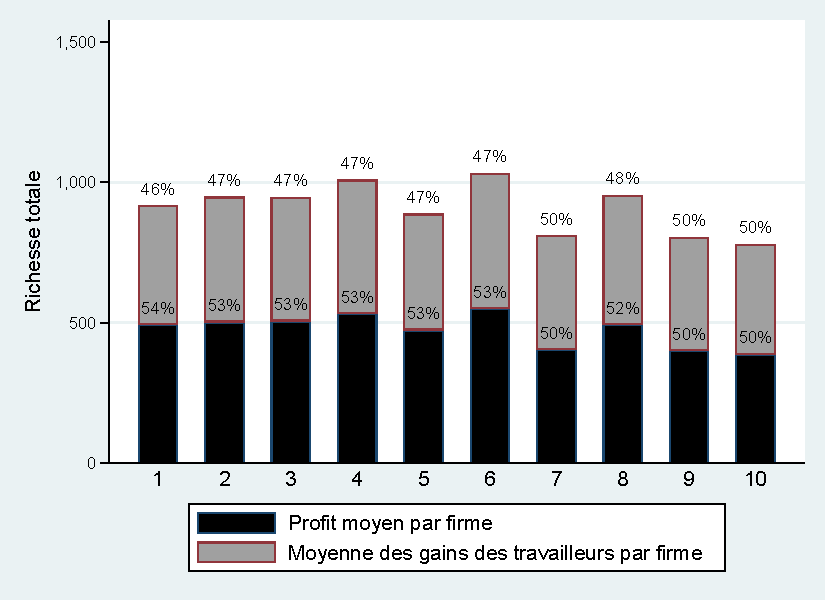
\includegraphics[height=6cm]{05_graphA8.pdf}
\end{figure}

\vspace{0.2cm}
La figure~A8 indique l'évolution de la répartition de la richesse
totale entre l'entreprise et les travailleurs au cours du temps dans le
traitement Baseline. Le partage de la richesse produite est relativement
égalitaire autour de 50~\% et ce ratio demeure stable au cours du temps.

\begin{figure}[h]
    \centering
    \caption{Évolution de la répartition de la richesse totale dans le traitement Pression des pairs}
    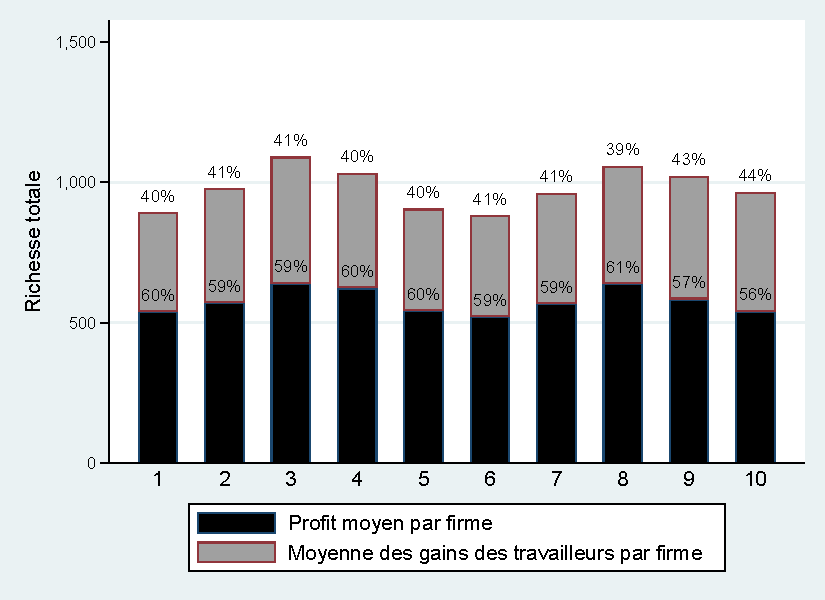
\includegraphics[height=6cm]{05_graphA9.pdf}
\end{figure}

La figure~A9 indique l'évolution de la répartition de la richesse
totale entre l'entreprise et les travailleurs au cours du temps dans le
traitement Pression des pairs. Le partage de la richesse produite est
légèrement en faveur de l'entreprise et ce ratio varie entre 56 et
61~\%. Ce ratio demeure assez stable au cours du temps.

\begin{figure}[h]
    \centering
    \caption{Évolution de la répartition de la richesse totale dans le traitement Objectif d'équipe}
    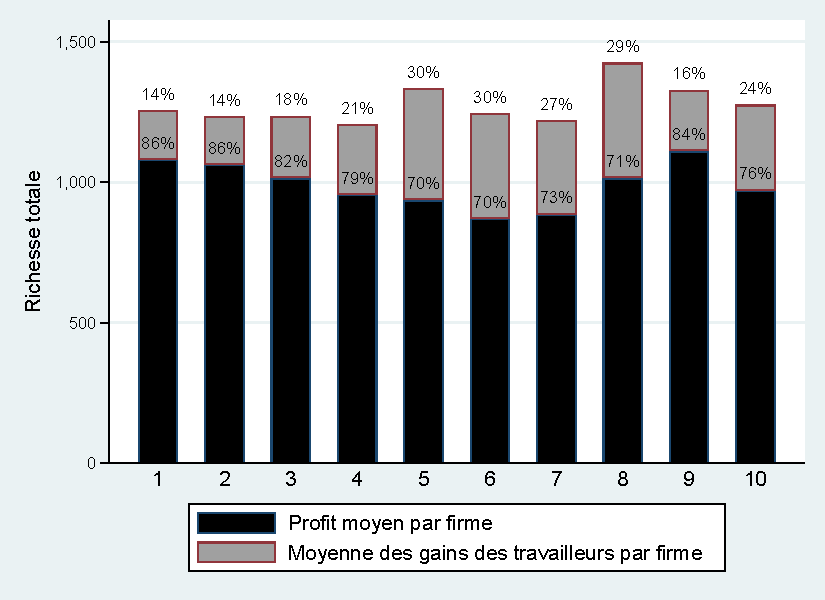
\includegraphics[height=6cm]{05_graphA10.pdf}
\end{figure}

La figure~A10 indique l'évolution de la répartition de la richesse
totale entre l'entreprise et les travailleurs au cours du temps dans le
traitement Objectif d'équipe. Le partage de la richesse produite est
très inégalitaire puisqu'elle est très largement en faveur de
l'entreprise et ce ratio varie entre 70 et 86~\%. On observe une légère
diminution de ce ratio au cours du temps.

\begin{figure}[h]
    \centering
    \caption{Évolution de la répartition de la richesse totale dans le traitement Tournois entre équipes}
    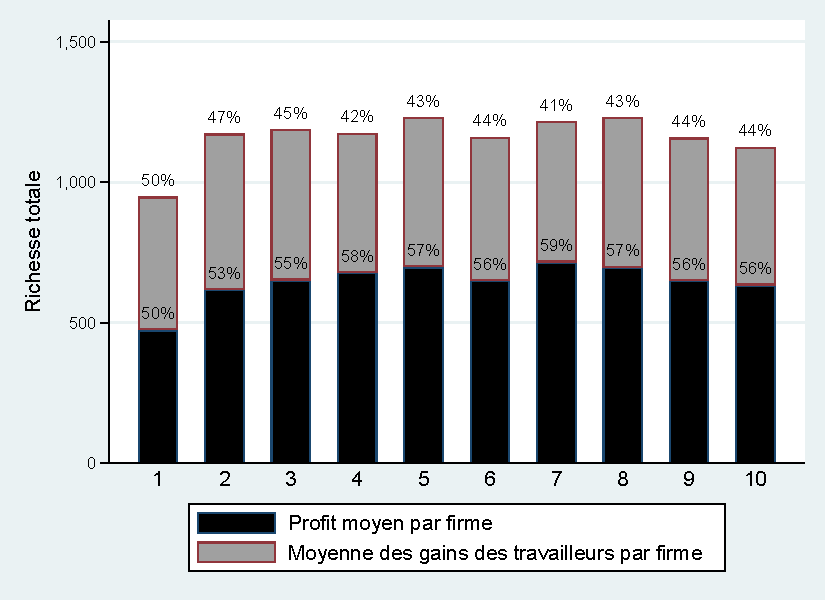
\includegraphics[height=6cm]{05_graphA11.pdf}
\end{figure}

La figure~A11 indique l'évolution de la répartition de la richesse
totale entre l'entreprise et les travailleurs au cours du temps dans le
traitement Tournois entre équipes. Le partage de la richesse produite
est assez égalitaire même s'il est légèrement en faveur de l'entreprise.
Ce ratio varie entre 50 et 59~\% et demeure assez stable au cours du
temps.

\end{appendices}

\end{refsection}

\end{Article}

% \graphicspath{{Articles-bons-a-composer/06_Mouminoux_al/06_Mouminoux_Figures/}}

\begin{Article}[Auteur={
    Claire Mouminoux\thanks{Université de Strasbourg, BETA. \emph{Correspondance~:} 61 avenue de la Forêt-Noire, 67000 Strasbourg, France. \emph{Courriel~:} mouminoux@unistra.fr}\\ 
    Morgane Plantier\thanks{Université de Poitiers, Laboratoire d'économie de Poitiers (LéP). \emph{Correspondance~:} 2 rue Jean Carbonnier, 86000 Poitiers, France. \emph{Courriel~:} morgane.plantier@univ-poitiers.fr}\\ 
    Jean-Louis Rullière\thanks{Université de Lyon, Université Claude Bernard Lyon 1, ISFA, Laboratoire SAF. \emph{Correspondance~:} 50 avenue Tony Garnier, 69000 Lyon, France. \emph{Courriel~:} jean-louis.rulliere@univ-lyon1.fr}}, 
    Titre={L'autoprotection influence-t-elle les choix d'assurance des individus ?\\ Une étude expérimentale}]

\label{Mouminoux}
  \selectlanguage{french}

\remerciements{Les auteurs remercient Romain Gauchon, Nathalie Havet, Meglena Jeleva, François Pannequin, les participants des Journées de Microéconomie Appliquée (JMA) 2023, ainsi que les deux rapporteurs anonymes de la \textit{Revue économique} pour leurs remarques et suggestions qui ont permis d'améliorer la qualité de l'article. Cette étude a bénéficié du soutien financier de la Chaire de recherche Prevent'Horizon. Toutes les erreurs ou omissions dans cet article restent propres aux auteurs.}

\begin{refsection}[Mouminoux]

\begin{resume}
À l'aide d'une expérimentation en laboratoire, cette étude compare les choix individuels en matière d’assurance, en fonction de la présence, ou non, d’une option d’autoprotection permettant de diminuer la probabilité de perte. Les résultats montrent que la possibilité d'engager un effort d'autoprotection, a posteriori, encourage les assurés à choisir des niveaux de couverture plus faibles, révélant ainsi leur préférence pour l'autoprotection par rapport à l'assurance. Cependant, les résultats indiquent également une incohérence dans les choix des individus puisque cet attrait pour l'option d'autoprotection ne se traduit finalement pas par davantage d'efforts d'autoprotection.    
\end{resume}

\titrearticleENG{Does self-protection affect individuals' insurance choice? An experimental study}

\begin{resumeENG}
Based on lab experiment, this study analyzes whether introducing a self-protection mechanism to reduce the loss probability affects individuals' insurance choices. The experimental evidence shows that the possibility of a posteriori self-protection encourages policyholders to choose lower levels of coverage, which reveals their preference for self-protection to mitigate their risk. However, this attraction to self-protection option does not turn into real action revealing an inconsistency of choices: individuals who deliberately choose to be less insured when a self-protection option is available do not subsequently engage in more self-protection efforts afterwards.
\end{resumeENG}

\motscles{assurance, autoprotection, expérimentation en laboratoire, biais hypothétique}

\keywords{insurance, self-protection, lab experiment, hypothetical bias}

\jelcode{D81, C91, D91}


\vspace{1cm}

\section{Introduction}

L'assurance et l'autoprotection sont des outils fondamentaux de gestion efficace des risques \parencite{WorldBank2013}. Alors que le premier vise à réduire le risque auquel les individus sont confrontés grâce au principe de mutualisation, le second a pour objectif de diminuer la probabilité d'occurrence du risque\footnote{En économie, deux principaux types de prévention sont généralement distingués \parencite{eb72} : l'\textit{Autoprotection} qui se réfère aux mesures visant à réduire la probabilité de survenance du risque, et l'\textit{auto-assurance} qui se réfère aux mesures visant à réduire l'ampleur de la perte dans le cas où le risque se réalise. Cependant, le second n'est pas l'objet de cette étude.}. Par exemple, dans le domaine de la santé, l'autoprotection peut faire référence à la pratique d'une activité physique pour réduire les risques cardiovasculaires, ou encore à l'adoption d'un programme nutritionnel sain réduisant le risque de survenue de certaines maladies. Ainsi, en diminuant le risque global, l'autoprotection implique des bénéfices importants, notamment pour les assurés. Du côté de l'assureur, les effets ne sont pas neutres pour autant : outre la réduction du risque global dans le portefeuille, si un pourcentage significatif des états préexistants est associé à une autoprotection insuffisante, l'augmentation des comportements d'autoprotection contribue à atténuer le poids de l'antisélection supporté par les assureurs\footnote{L'antisélection désigne le fait que les individus ajustent leur niveau d'assurance en fonction de leur propre évaluation du risque, une information qu'ils détiennent de manière privée. Lorsque les assureurs ne peuvent pas intégrer cette donnée dans leur modèle de tarification, l'antisélection peut conduire à l'insoutenabilité du marché de l'assurance \parencite{rs76}.}.

D'un point de vue théorique, en économie de l'assurance, l'examen des comportements individuels d'autoprotection est généralement réalisé en termes d'interaction avec les choix d'assurance et peut donc être abordé sous l'angle de l'aléa moral. Dans la relation principal-agent qui existe entre l'assureur et l'assuré, l'effet d'aléa moral désigne l'effet désincitatif de l'assurance qui motive l'assuré à se détourner des activités d'autoprotection. Par exemple, les personnes ayant une assurance automobile peuvent conduire de manière plus imprudente car elles se sentent protégées en cas d'accident \parencite{Arrow1963,Arrow1968,p68}. Selon cette hypothèse, l'assurance et l'autoprotection sont négativement corrélées. Cependant, certaines études ont exprimé des réserves quant à la robustesse empirique de cette prédiction théorique \parencite{cs00}. En particulier, sous l'hypothèse d'une hétérogénéité dans les préférences individuelles (par exemple, les préférences en matière de risque), la relation entre l'assurance et le comportement d'autoprotection pourrait être inversée : un individu ayant une forte aversion au risque pourrait exprimer une forte demande d'assurance pour limiter sa perte financière et également, dans le même temps, exercer des efforts d'autoprotection plus importants pour réduire la probabilité de survenue du risque \parencite{cjss06,dh09,dw01,h90,h92}. Cet argument fait référence à la notion de \textit{sélection avantageuse} (ou \textit{avantageous selection}), qui pourrait expliquer l'existence d'une corrélation positive entre l'assurance et l'autoprotection.

D'un point de vue empirique, cette absence de consensus quant à la nature de la relation entre ces deux outils de gestion du risque demeure. Les travaux présents dans la littérature prennent deux formes principales, qui dépendent du type de données mobilisées. Faute de pouvoir observer simultanément les décisions individuelles en matière d'assurance et d'autoprotection, ou encore de pouvoir construire un contrefactuel crédible permettant l'identification d'une relation de causalité, une première catégorie de travaux s'est intéressée à la relation entre le niveau d'assurance et le niveau de risque final. Dans ce cadre, sous l'hypothèse que le niveau de risque observé des individus est déterminé par deux dimensions, leurs caractéristiques individuelles et leur comportement vis-à-vis de ce risque, une fois contrôlé de la première, le niveau de risque peut être considéré comme un indicateur du niveau d'effort d'autoprotection fourni par les individus pour diminuer ce risque (un risque final élevé sera donc révélateur d'un effort d'autoprotection faible, et inversement). À partir de cette hypothèse, les nombreuses études qui ont analysé la relation entre le niveau d'assurance et le niveau de risque ont donné lieu à des résultats mitigés. Certains travaux révèlent une corrélation positive entre le niveau de couverture assurantielle et le niveau de risque, conformément à l'hypothèse d'aléa moral (\textcite{c05,ps94,r99} examinent le marché de l'assurance automobile, alors que \textcite{bcgp04} se concentrent sur le marché de l'assurance santé). D'autres concluent à l'absence d'une corrélation entre l'assurance et le niveau de risque, réfutant l'hypothèse d'un réel arbitrage entre assurance et autoprotection (\textcite{cs00} et \textcite{s06} se concentrent sur le marché de l'assurance automobile et \textcite{ch01} sur le marché de l'assurance santé). Enfin, certains aboutissent à l'observation d'une corrélation négative entre l'assurance et le niveau de risque, révélatrice d'une relation inverse entre l'assurance et l'autoprotection (\textcite{fm06} analysent le marché de l'assurance de soins de longue durée, \textcite{hl03} celui de l'assurance vie, et \textcite{bfjs13}, \textcite{cc17} et \textcite{fks08} étudient le cas de l'assurance santé).

Une seconde catégorie de travaux s'est quant à elle prêtée à l'exercice de l'analyse de l'arbitrage entre l'assurance et l'autoprotection à partir d'observations concernant ces deux éléments, lorsque celles-ci étaient disponibles. Même s'ils sont beaucoup moins nombreux et concernent principalement le marché de l'assurance santé, les résultats restent également ambigus. D'un côté, certains travaux valident par exemple l'hypothèse de comportements d'aléa moral sur les marchés de l'assurance santé mexicain et américain (\textcite{s12} ; \textcite{s08}) ; alors que, d'un autre côté, des études mettent en avant le résultat inverse en montrant que les individus les mieux assurés sont également ceux qui adoptent les comportements les plus sains vis-à-vis du risque santé (par exemple, ne pas consommer d'alcool ou de cigarettes, rester en forme, etc.) \parencite{cd04,cl10,ff09,k94}. Les résultats semblent varier selon le contexte, et le marché d'assurance considéré.

Dans ce cadre, et compte tenu de la contrainte forte liée à la qualité des données disponibles, l'approche expérimentale apparaît comme un outil approprié pour analyser les arbitrages individuels entre l'assurance et l'autoprotection. Toutefois, si la question des déterminants de la demande individuelle d'assurance a déjà été abordée en économie comportementale (voir \textcite{j16} pour une synthèse des travaux expérimentaux), les travaux expérimentaux qui incluent également la notion d'autoprotection restent parcimonieux\footnote{Quelques études expérimentales ont analysé la relation entre l'assurance et l'auto-assurance. Par exemple, \textcite{pcm20} mettent en évidence une relation de substituabilité entre ces deux outils de gestion des risques. De même, \textcite{mbb20} concluent à l'existence d'un phénomène d'aléa moral entre l'assurance et l'auto-assurance, marqué par une forte hétérogénéité en fonction de la probabilité de perte.}. Seuls les travaux de \textcite{bct15} et \textcite{p22} analysent les décisions individuelles d'assurance et d'autoprotection dans le cadre d'une expérimentation en laboratoire. Les premiers examinent le rôle de l'ambiguïté sur l'arbitrage entre ces deux outils de gestion des risques et montrent notamment que l'ambiguïté incite les participants à privilégier l'outil assurantiel. Les seconds s'intéressent à l'impact de la nature du contrat d'assurance, entre un contrat choisi et un contrat imposé, sur le niveau d'effort d'autoprotection consenti par les individus, et concluent à un impact négatif de l'introduction de l'option de choix du contrat sur les comportements d'autoprotection des assurés.

L'objectif principal de cette étude est d'examiner empiriquement l'effet de l'autoprotection sur les décisions individuelles en matière d'assurance. Alors que les recherches précédentes se sont principalement concentrées sur la manière dont l'assurance affecte les comportements d'autoprotection, cette étude expérimentale propose de poser la question inverse : l'introduction d'une option d'autoprotection influence-t-elle les choix d'assurance des individus ? Cette étude offre de nouveaux résultats empiriques complémentaires sur la relation entre l'assurance et l'autoprotection. De plus, elle s'inscrit dans un contexte où un nombre croissant d'assureurs cherchent à intégrer l'autoprotection dans leur offre. Par exemple, en France, dans le domaine de la santé, de nombreux assureurs envisagent de proposer une option d'autoprotection qui serait incluse dans les contrats d'assurance santé complémentaire (par exemple, rembourser l'abonnement à la salle de sport, offrir une visite annuelle chez un spécialiste, etc.). Ainsi, comprendre les impacts potentiels de l'introduction de l'autoprotection sur les choix individuels en matière d'assurance représente des enjeux importants. Pour aborder cette question empirique, deux traitements expérimentaux impliquant un choix d'assurance obligatoire parmi un menu de plusieurs contrats, avec l'option (ou non) de réaliser un effort d'autoprotection coûteux afin de réduire la probabilité de perte, ont été comparés. Dans les deux cas, les assureurs ne peuvent pas observer les activités d'autoprotection des individus, laissant place à un potentiel effet d'aléa moral. La comparaison de ces deux traitements va ainsi permettre d'identifier l'impact de l'introduction d'une option d'autoprotection sur les choix d'assurance des individus dans un environnement dynamique où les décisions d'assurance et d'autoprotection se produisent de manière séquentielle (choix d'assurance d'abord, suivi par l'effort d'autoprotection).

Alors que les prédictions théoriques indiquent qu'aucune différence en matière de choix d'assurance ne devrait être observée entre les différents traitements (avec ou sans l'option d'autoprotection), les données expérimentales montrent pourtant que l'introduction d'un mécanisme d'autoprotection diminue la demande d'assurance des participants. Ce premier résultat empirique révèle ainsi un attrait pour le mécanisme visant à diminuer la probabilité de perte --~l'autoprotection~-- par rapport à l'assurance, en faveur de l'hypothèse de substituabilité entre les deux outils de gestion des risques. Ce premier résultat a ensuite conduit à analyser les efforts d'autoprotection consentis par les participants, afin de comprendre comment cette préférence pour l'autoprotection se manifeste et, en particulier, si les arbitrages individuels entre l'assurance et l'autoprotection s'avèrent cohérents (bien que non alignés sur les prédictions théoriques). En d'autres termes, il a été question de vérifier si les individus, qui ont volontairement diminué leur demande d'assurance en présence du mécanisme d'autoprotection, ont ensuite fourni davantage d'efforts pour diminuer la probabilité d'occurrence du risque. Pour ce faire, un troisième traitement a été mis en \oe uvre dans le but d'analyser les comportements d'autoprotection, dans lequel le contrat d'assurance est imposé aléatoirement. Les résultats révèlent une incohérence des choix individuels : les participants qui ont choisi de moins s'assurer en raison de la présence de l'option d'autoprotection, ne fournissent pas davantage d'efforts pour diminuer la probabilité de perte ensuite. En d'autres termes, l'attrait pour l'autoprotection observé dans la première étape ne semble pas se traduire par un réel effort d'autoprotection par la suite. 

Cet article est organisé comme suit. La section \ref{section:experimentation} décrit la méthode expérimentale, la section \ref{section:resultats} présente les résultats et la section \ref{section:conclusion} discute et conclut. \\


\section{L'expérimentation}
\label{section:experimentation}

\subsection{Le modèle théorique}

Dans le cadre d'un modèle simplifié de demande d'assurance, les individus disposent d'un niveau de richesse initial identique $W$ et font face à un risque de perte monétaire d'un montant $L$, avec une probabilité $\bar{p}$ (avec $0 < \bar{p} < 1$). $W$, $L$ et $\bar{p}$ sont supposés parfaitement connus.

Chaque individu a accès à deux outils de gestion des risques : 1)~un contrat d'assurance parmi un menu de $J$ alternatives, qui  permet de bénéficier d'une indemnisation en cas de perte en contrepartie du paiement d'une prime d'assurance quelle que soit la réalisation de l'état de la nature ; et 2)~un mécanisme d'autoprotection, qui  permet de réduire la probabilité de perte. La souscription à un contrat d'assurance est obligatoire, tandis que les mesures d'autoprotection sont facultatives.

Chaque contrat d'assurance se compose d'une prime $CP$, qui garantit une indemnité $I$ en cas de perte, avec $I=\alpha L$, où $\alpha$ désigne le taux de couverture du contrat. Comme proposé initialement par \textcite{m68}, puis popularisé par \textcite{s00}, la prime d'assurance peut être écrite comme suit :

\begin{equation}
\label{eq:premium}
CP = \alpha(1+\lambda)\bar{p}L,
\end{equation}

\noindent où $\lambda$ désigne le taux de chargement du contrat. L'assureur ne peut pas observer l'effort d'autoprotection effectué par l'assuré pour réduire sa probabilité de perte, il est supposé conservateur et n'anticipe aucun effort d'autoprotection lors de la détermination du niveau de prime. Par conséquent, le montant de la prime $CP$ dépend uniquement de la probabilité de perte initiale $\bar{p}$.

Une fois qu'un contrat d'assurance est sélectionné, chaque assuré peut faire un effort d'autoprotection $e$ pour réduire sa probabilité de perte $\bar{p}$ (avec $e \ge 0$). La probabilité de perte finale devient $p(e)$, qui est une fonction affine décroissante en $e$: $p(e)=\bar{p} - a e$, avec $a$ une constante réelle positive\footnote{Une relation linéaire entre l'effort $e$ et la probabilité de perte $p(e)$ a été choisie principalement pour des raisons pratiques, afin de permettre la compréhension et l'appropriation du mécanisme d'autoprotection par les participants (ce choix a été motivé à la suite de la mise en \oe uvre de sessions pilotes). De plus, une fonction non linéaire aurait nécessité l'affichage d'un tableau de valeurs qui aurait pu induire un effet de cadrage.}. Le coût de l'effort d'autoprotection est représenté par une fonction de coût monétaire linéaire $c(e)$, telle que $c(e)=c e$. \textcite{Araujo_etal2016}, \textcite{cgh18} et \textcite{gp19} ont mis en évidence les limites d'une mesure d'effort réel en laboratoire et les conséquences sur les résultats. Dans ce cadre, une fonction de coût monétaire a été privilégiée pour représenter le coût de l'autoprotection afin de garantir le même accès au mécanisme d'autoprotection pour tous les individus et donc la comparabilité des résultats. $c(e)$ et $p(e)$ sont supposés parfaitement connus par l'assuré.

Finalement, les individus sont supposés maximiser leur utilité espérée. Ils ne diffèrent que par leur préférence en matière de risque, qui se reflète par des différences dans leur fonction d'utilité $U(.)$. Formellement, les individus maximisent l'utilité espérée suivante :
\begin{gather}
E(U(\alpha,e)) = p(e)U[W - c(e) -\alpha(1+\lambda)\bar{p}L - (1 - \alpha)L] \notag \\+ (1 - p(e))U[W - c(e) - \alpha(1 + \lambda)\bar{p}L],
\end{gather}

\noindent sous contrainte que $0 \le e \le \bar{e}$ et $\underline \alpha \le \alpha \le \bar \alpha$, avec $\bar{e}$ le niveau d'effort maximal d'autoprotection réalisable, $\underline \alpha$ et $\bar \alpha$, les taux de couverture d'assurance minimum et maximum proposés dans le menu de contrats.


\subsection{Le design expérimental}

À partir du modèle de demande d'assurance décrit précédemment, la procédure expérimentale retenue permet de comparer les choix individuels en matière d'assurance en présence, ou non, d'une option d'autoprotection. Chaque session expérimentale se compose de trois parties distinctes. Le c\oe ur de l'expérimentation est contenu dans la deuxième partie et concerne le choix d'un contrat d'assurance, avec ou sans mécanisme d'autoprotection. La première et la troisième parties contiennent des tâches supplémentaires nécessaires pour contrôler certaines variables individuelles (dotations initiales et aversion au risque). Contrairement à de nombreuses études expérimentales menées dans le domaine de l'assurance, la formulation utilisée pour les instructions reste neutre et indépendante de tout contexte. En particulier, les termes suivants ne sont jamais mentionnés aux participants : assurance, autoprotection (ou prévention), prime et indemnisation. Ce choix a été motivé par le fait de garantir un environnement neutre afin d'analyser spécifiquement les mécanismes sous-jacents aux stratégies de gestion des risques employées par les individus, sans que ceux-ci ne soient influencés par les connotations préexistantes associées aux termes cités précédemment. Les unités monétaires sont exprimées en \textit{Experimental Currency Units} (ECU), avec le taux de conversion suivant : 100 ECU = 1 euro. Ce taux de conversion est communiqué aux participants au début de l'expérimentation et utilisé pour définir le paiement final.

\subsubsection{Choix d'assurance et d'autoprotection}

Pour modéliser les choix individuels en matière d'assurance et d'autoprotection, chaque participant est exposé à 12~situations de risque différentes (12~périodes indépendantes), correspondant à un jeu de hasard dans lequel il fait face à une urne électronique contenant 100~boules, chacune de couleur bleue ou rouge. Le jeu, inspiré de la procédure proposée par \textcite{sflcc77} et également utilisée par \textcite{lms09} et \textcite{bct15}, consiste en un tirage aléatoire d'une des boules contenues dans l'urne et qui sera directement effectué par l'ordinateur. En cas de tirage d'une boule rouge, le participant subit une perte monétaire ($L$) qui sera prélevée de sa richesse initiale ($W = 1500$). En cas de tirage d'une boule bleue, le participant ne subit aucune perte et conserve l'intégralité de cette richesse. Deux niveaux de risque sont considérés. Dans le premier cas, l'urne contient 20 boules rouges et 80 boules bleues (soit $\bar{p}=0,2$, la probabilité \textit{faible}), alors que dans le second cas, l'urne contient 50 boules rouges et 50 boules bleues (soit $\bar{p}=0,5$, la probabilité \textit{élevée}). Les niveaux de risque ont été choisis à partir de la littérature existante (\textcite{sflcc77}; \textcite{lms09}; \textcite{bct15})\footnote{Ces études expérimentales ont retenu des probabilités de perte allant de 0,0001 à 0,5.}. Concernant le montant de la perte en cas de tirage d'une boule rouge, deux cas sont également considérés : une perte de 600~ECU (soit $L=600$, le montant \textit{faible}), ou une perte de 1500~ECU (soit $L=1500$, le montant \textit{élevé}). La perte de l'intégralité de la richesse initiale fait donc partie des possibilités (\textcite{lms09}; \textcite{bct15}). Pour chacune des 12~périodes, chaque participant a connaissance, dès le début du jeu, du montant de sa richesse initiale (1500~ECU, réinitialisée au début de chaque période), du montant de la perte potentielle (600~ECU ou 1500~ECU) et de la composition de l'urne (c'est-à-dire de la répartition du nombre de boules bleues et rouges)\footnote{Au début du jeu, l'écran affiche simultanément l'urne électronique, avec la répartition des boules des deux couleurs, et la description du contenu (voir l'exemple figurant dans les instructions reportées en annexe \ref{Annexe:Instruction}).}. Une fois le participant informé de l'ensemble de ces caractéristiques, le choix se déroule en deux étapes successives.

\vspace{0,3cm}
\textit{Étape 1 : Choix d'assurance}

\vspace{0,2cm}
Chaque participant doit choisir un contrat d'assurance (obligatoire) à partir d'un menu de quatre alternatives, qui lui permet de bénéficier d'une indemnisation en cas de tirage d'une boule rouge en échange d'une prime d'assurance (payée même en l'absence de perte). À chaque période, le menu est composé de quatre contrats qui ne diffèrent que par leur taux de couverture $\alpha$, avec $\alpha = \{0,40;0,65;0,80;0,90\}$\footnote{Le cas d'une couverture complète ($\alpha = 1$) est exclu afin de conserver le mécanisme d'autoprotection pertinent (en cas d'une couverture assurantielle complète, l'autoprotection disparaît totalement).}. Les quatre niveaux de couverture possibles, qui permettent de mesurer l'effet de sélection de manière non linéaire, restent les mêmes pour toutes les périodes. Par ailleurs, trois taux de chargement sont considérés : $\lambda = \{-0,2;0;0,2\}$, avec $\lambda=-0,2$ qui correspond à un contrat subventionné\footnote{Par exemple, ce type de contrats correspond au marché de l'assurance santé subventionné par l'État dans de nombreux pays développés.}, $\lambda = 0$ qui correspond à la prime actuarielle, et $\lambda = 0,2$ qui correspond à un contrat chargé.  Le choix de $\lambda = 0,2$ est motivé par les pratiques des assureurs français. En effet, le ratio moyen de perte pour les compagnies d'assurance françaises est d'environ 80~\% \parencite{fa22}\footnote{Le ratio de perte correspond au rapport entre les indemnisations versées et les primes perçues.}. Le choix de la symétrie pour le cas de l'assurance subventionnée est quant à lui motivé par le fait de rendre comparable ces deux cas. La prise en compte de ces trois cas va permettre de tester si le taux de chargement du contrat d'assurance a un impact sur les décisions des participants en termes d'assurance et d'autoprotection. Finalement, pour chaque période, le taux de chargement est le même pour les quatre niveaux de couverture proposés et la prime d'assurance est définie selon l'équation (\ref{eq:premium}).

\newpage
\textit{Étape 2 : Choix d'autoprotection}

\vspace{0,2cm}
La modélisation de l'effort d'autoprotection consiste à donner, à chaque participant, la possibilité de remplacer des boules \textit{risquées} (rouges) par des boules \textit{non risquées} (bleues). Chaque remplacement est associé à un coût unitaire qui correspond au coût monétaire de l'effort d'autoprotection $c$\footnote{Il correspond au coût associé à une diminution d'un point de pourcentage de la probabilité de perte.}. Par ailleurs, l'effort d'autoprotection est limité au maximum à 15~remplacements de boules rouges par des boules bleues ($\bar{e} = 15$). D’une part, cette limite permet d’exclure tout paiement final négatif, garantissant ainsi la faisabilité du jeu. D’autre part, ce plafonnement implique le fait que l'effort d'autoprotection ne permet pas de réduire la probabilité de perte à 0\footnote{$p(\bar{e}) = 0,35$ en cas de probabilité de perte initiale élevée ($\bar{p} = 0,5$) et $p(\bar{e}) = 0,05$ en cas de probabilité de perte initiale faible ($\bar{p} = 0,2$).}. Ce niveau maximal d'effort d'autoprotection est le même pour chaque période afin d'éviter les effets de cadrage. Finalement, deux niveaux de coût unitaire de remplacement $c$ sont considérés :  $c=6$, le coût \textit{faible} (qui, par construction, est associé au montant de perte faible ($L=600$)), et $c=15$, le coût \textit{élevé} (qui, par construction, est associé au montant de perte élevée ($L=1500$))\footnote{$c(e)$ a été spécifiée de sorte que le coût d'un effort d'autoprotection qui permettrait de réduire la probabilité de perte à 0 soit équivalent au coût d'une couverture hypothétique complète ($\alpha=1$) au prix actuariel ($\lambda =0$), soit : $\frac{\bar p}{0,01}\times c=\bar p \times L$.}. Les participants reçoivent les informations concernant le coût unitaire et le niveau d'effort maximal d'autoprotection au début de chaque période, c'est-à-dire avant de choisir un contrat d'assurance puis un niveau d'effort d'autoprotection.

Ces deux étapes sont jouées de manière séquentielle par les participants (étape~1 puis étape~2). Ils sont informés, dès le début du jeu, de toutes les décisions qu'ils auront à prendre et des caractéristiques associées (la probabilité de perte initiale ($\bar{p}$), le montant de la perte ($L$), la taille du menu de contrats d'assurance ($J$), le nombre de remplacements de boules rouges par des boules bleues possibles ($\bar{e}$), et le coût unitaire de chaque remplacement ($c$)). L'introduction de la séquentialité et, en particulier, l'ordre des deux choix à effectuer --~choix d'assurance puis d'autoprotection~-- a pour objectif de permettre des analogies avec des situations concrètes impliquant le choix d'un contrat d'assurance (choix du niveau de couverture), qui inclurait une option d'autoprotection disponible après souscription (par exemple, un contrat d'assurance santé offrant un accès facilité au sport en couvrant une partie des frais d'une adhésion sportive).

Finalement, 12~périodes différentes et indépendantes, comprenant les étapes~1 et 2, sont proposées à chaque participant. Plus précisément, les 12~périodes correspondent à la combinaison des différents paramètres considérés, qui sont résumés dans le tableau 1\footnote{Les paramètres sont contraints pour garantir des paiements non négatifs ($W-P-L+ I - c(\bar{e}) \ge 0 $, avec $P= \alpha(1+\lambda)\bar pL$ et $I= \alpha L$).}. L'ordre des périodes a été défini de manière aléatoire et est identique pour tous les participants dans chaque session afin d'éviter les effets d'ordre\footnote{Préalablement, deux exemples d’entraînement sont proposés pour que chaque participant puisse se familiariser avec l’interface.}. Le paiement final du jeu principal est déterminé selon une procédure de \textit{random incentive lottery} : une fois l’ensemble des périodes jouées, une seule est tirée au sort, le risque est joué et le paiement final est déterminé en fonction des décisions effectuées par le participant durant cette période. L’avantage de cette procédure est d’éviter un potentiel effet de portefeuille et de maintenir l’attention des participants jusqu’à la fin du jeu \parencite{cgh16}.

{\tabletextsize
  \begin{longtable}[c]{clr}
    \caption{Valeurs des paramètres}
    \label{tab:parameters}\\
    
    \toprule
    Paramètre&Définition&Valeurs\\
    \midrule
    \endfirsthead
    
    \midrule
    Paramètre&Définition&Valeurs\\
    \midrule
    \endhead
    
    \midrule
    \endfoot
    
    \bottomrule
    \endlastfoot
    $T$&Nombre de périodes&12\\
    $W$&Richesse initiale&1500\\
    $\bar{p}$&Probabilité de perte&\{0,2 ; 0,5\}\\
    $L$&Montant de la perte&\{600 ; 1500\}\\
    $J$&Taille du menu&4\\
    $\alpha$&Taux de couverture&\{0,4 ; 0,65 ; 0,80 ; 0,90\}\\
    $e$&Effort d'autoprotection&\{0,1, \ldots,15\}\\
    $\lambda$&Taux de chargement&\{-0,2 ; 0 ; 0,2\}\\
    $c(e)$&Fonction de coût d'autoprotection&$c(e)=c e $ avec $
    c = \{6 ; 15\}$\\
    $p(e)$&Fonction de diminution du risque &$p(e)=\bar{p} - a e $ avec $ a=0,01$\\
    \end{longtable}
}

Le design expérimental a été décliné en trois traitements différents, qui incluent les mêmes menus de contrats et les mêmes paramètres pour chaque période :

\begin{itemize}
    \item \textit{Traitement Assurance + autoprotection} : les participants doivent choisir un contrat d'assurance obligatoire parmi un menu de quatre contrats (étape~1), puis décider du nombre de boules rouges qu'ils veulent remplacer par des boules bleues (étape~2).

    \item \textit{Traitement Assurance} : les participants doivent choisir un contrat d'assurance obligatoire parmi un menu de quatre contrats (étape~1). Il s'agit de la seule tâche de ce traitement. Le mécanisme d'autoprotection n'existe pas et n'est pas mentionné.

    \item \textit{Traitement Autoprotection} : un contrat d'assurance obligatoire est attribué à chaque participant (sélectionné de manière aléatoire au niveau individuel parmi les quatre mêmes contrats offerts dans les autres traitements). Ils reçoivent des informations sur le contrat qui leur a été imposé (étape~1), puis peuvent choisir le nombre de boules rouges qu'ils souhaitent remplacer (étape~2). \\

\end{itemize}

Le tableau 2 résume les options disponibles dans les trois traitements.

% Tableau 2

{\tabletextsize
\begin{longtable}[c]{L{2cm}L{2cm}cL{2cm}}
  \caption{Description des options disponibles selon les traitements}
  \label{tab:treatment_option} \\
  \toprule
         Traitement & Choix de l'assurance & Taux de couverture & autoprotection \\
  \midrule
  \textit{Assurance + autoprotection} & Choix du contrat  &  $\alpha \in \{0,40;0,65;0,80;0,90\}$ & Disponible \\
  \textit{Assurance} & Choix du contrat &  $\alpha \in \{0,40;0,65;0,80;0,90\}$ & Non disponible \\
  \textit{Autoprotection} & Contrat imposé &  $\alpha \in \{0,40;0,65;0,80;0,90\}$ & Disponible \\
  \bottomrule
  \end{longtable}}

\subsubsection{Résultats attendus}

À partir du modèle théorique décrit précédemment, la prise de décisions d'un agent rationnel est supposée suivre la théorie de l'utilité espérée, étant donné les paramètres de chaque période et pour chacun des traitements. Le tableau 3 résume les programmes d'optimisation et les variables de décisions correspondants à chaque traitement.

% Tableau 3

\begin{table}[h!]
  \caption{Description des programmes d'optimisation selon les traitements}
    \label{tab:treatment_opti} 
  \begin{tabular}[c]{lcC{3cm}}
    \toprule
           Traitement & Programme d'optimisation & Variables de décision \\
    \midrule
    \textit{Assurance + autoprotection} & $(\alpha^*,e^*) = \arg\max~EU(\alpha,e)$ & $\alpha \in \{0,40;0,65;0,80;0,90\}$ et $0 \le e \le 15$ \\
    \textit{Assurance} & $\alpha^* = \arg\max~EU(\alpha,0)$ &$ \alpha \in \{0,40;0,65;0,80;0,90\}$\\
    \textit{Autoprotection} & $e^* = \arg\max~EU(\bar{\alpha} ,e)$ &  $0 \le e \le 15$\\\bottomrule
    \end{tabular}
    \notedetableau{$\bar{\alpha}$ est attribué à chaque participant de manière aléatoire, avec une probabilité équivalente ($1/4$) parmi les valeurs possibles de $\alpha \in \{0,40; 0,65; 0,80; 0,90\}$.}   
\end{table}

Premièrement, la résolution algébrique pour le traitement \textit{Assurance} correspond à celle proposée par \textcite{s00}, où aucun effort d'autoprotection n'est possible. Dans ce cadre, plus les individus sont averses au risque, plus ils choisissent une couverture élevée, quelle que soit la valeur de $\lambda$. Concernant les individus neutres vis-à-vis du risque, ils seront indifférents entre les différents taux de couverture proposés dans le cas d'une prime actuarielle ($\lambda=0$), ils choisiront le taux de couverture le plus faible dans le cas d'une prime chargée ($\lambda>0$) et le taux de couverture le plus élevé dans le cas d'une prime subventionnée ($\lambda<0$). Enfin, pour les individus risquophiles, ils choisiront toujours la couverture la plus faible dans le cas d'une prime actuarielle ou chargée ($\lambda \geq 0$). Lorsque la prime est subventionnée ($\lambda < 0$), ils pourront être amenés à choisir le taux de couverture le plus élevé. Cela est d'autant plus vrai que la subvention est élevée et que leur degré d'appétence pour le risque est faible. Par ailleurs, les effets du niveau de probabilité de perte initiale ($\bar{p}$) et du montant de la perte ($L$) sur les choix individuels d'assurance ne sont pas monotones et dépendent de la forme de la fonction d'utilité et de la combinaison des deux paramètres.
 
Deuxièmement, concernant les deux autres traitements (\textit{Assurance} +\linebreak \textit{Autoprotection} et \textit{Autoprotection}), la solution algébrique peut être partiellement obtenue en utilisant l'induction récursive (\textit{backward induction}). Une expression explicite peut être obtenue pour les individus neutres vis-à-vis du risque et les risquophiles, quelle que soit la forme de la fonction d'utilité. En particulier, ces agents n'ont jamais intérêt à fournir un effort d'autoprotection. Autrement dit, le niveau optimal d'autoprotection est toujours égal à 0 ($e^*(\alpha)=0,\ \forall \alpha$). Concernant le niveau de couverture assurantielle, il dépend du taux de chargement. Plus précisément, une augmentation du taux de chargement implique une diminution du niveau de couverture optimal parmi les alternatives disponibles ($\frac{\partial \alpha^*}{\partial \lambda} \le 0$). Ce résultat tient compte du fait que la souscription à un contrat d'assurance est obligatoire, qu'une couverture complète n'est jamais disponible et que l'effort d'autoprotection n'est pas observable par l'assureur. Concernant les individus averses au risque, bien que les conditions du premier ordre soient facilement identifiées, la résolution nécessite la spécification de la fonction d'utilité ainsi que des paramètres individuels associés. Ainsi, le recours à des simulations numériques, nécessitant des hypothèses sur la forme de la fonction d'utilité et les paramètres associés, a été nécessaire afin de déterminer les choix optimaux théoriques en matière d'assurance et d'autoprotection pour les individus averses aux risque\footnote{L'ensemble des détails de la résolution algébrique, pour les trois cas étudiés, sont fournis dans l'annexe \ref{Annexe:Expected_results_theo}.}.

Pour ce faire, différentes formes de fonctions d'utilité et de paramètres associés à la préférence vis-à-vis du risque ont été considérés afin de calculer les choix optimaux d'assurance et d'autoprotection pour chaque période, selon chacun des traitements, à partir des programmes d'optimisation décrits dans le tableau 3\footnote{Le code R qui a été utilisé est disponible sur demande auprès des auteurs.}. Tout d'abord, une fonction d'utilité de type CRRA (à aversion relative au risque constante ou \textit{constant relative risk aversion}) ou DARA (à aversion absolue au risque décroissante ou \textit{decreasing absolute risk aversion}) a été utilisée, soit : 
\begin{equation}
U(x) = \left\{
    \begin{array}{ll}
        \frac{x^{(1-r)}}{1-r} & \mbox{si } r \neq 1 \\
        \ln(x) & \mbox{sinon,}
    \end{array}
\right.
\end{equation}
avec $r$ qui correspond au paramètre d'aversion au risque, tel que $r \in [0,~3]$\footnote{\textcite{hl02} classent les individus pour $r \in [-3,~3]$, avec $r \in [-3,~0]$ qui correspond au cas des individus neutres vis-à-vis du risque et risquophiles (cas traité précédemment) et $r \in [0,~3]$ au cas des individus averses au risque.}.

Ainsi, pour les individus averses au risque, sur la base des hypothèses retenues, les résultats obtenus correspondent à ceux trouvés pour les individus neutres au risque et risquophiles. En particulier, l'effort optimal d'autoprotection est à nouveau nul, soit $e^*(\alpha)=0, \forall \alpha$, le niveau de couverture optimal dépend négativement du taux de chargement, soit $\frac{\partial \alpha^*}{\partial \lambda}<0$, et, conformément aux résultats de \textcite{m68} et \textcite{s00}, le niveau de couverture optimal dépend positivement du niveau d'aversion au risque, soit $\frac{\partial \alpha^*}{\partial r}>0$\footnote{Pour le calcul numérique, l'ensemble des variables de décisions a été limité aux choix discrets retenus pour l'expérimentation ($\alpha = \{0,40;0,65;0,80;0,90\}$ et $0 \le e \le 15$).}.

Cependant, l'utilisation d'une fonction d'utilité de type CRRA ou DARA peut s'avérer trop restrictive. Aussi, un test de sensibilité des résultats a été effectué en utilisant une fonction d'utilité de type \og \textit{power-expo}\fg, comme proposé par \textcite{hl02}, permettant de calculer les résultats théoriques pour les individus averses au risque présentant une aversion relative au risque décroissante et croissante. Les résultats précédemment décrits restent à nouveau valables\footnote{Le détail des hypothèses retenues pour effectuer ce test de sensibilité est reporté dans l'annexe~\ref{Annexe:Expected_results_num}.}.

Finalement, l'ensemble de ces résultats conduisent à définir un résultat principal attendu : l'introduction d'une option d'autoprotection, dans une seconde étape, ne devrait pas modifier le choix de couverture effectué par les individus en première étape \footnote{Ce résultat principal est une des conséquences directes du choix des paramètres de l'expérimentation. Plus précisément, les résultats théoriques décrits précédemment indiquent que $e^*(\alpha) = 0, \forall \alpha$, quels que soient le traitement et le niveau de préférence vis-à-vis du risque. Ce résultat permet de faciliter l'identification d'un potentiel effet de l'introduction d'une option d'autoprotection et également de faciliter les interprétations dans le cadre d'un design \textit{between-subject} comme c'est le cas ici.}. Autrement dit, aucune différence ne devrait être observée en termes de niveaux de couverture d'assurance choisis par les participants entre les traitements \textit{Assurance} et \textit{Assurance + autoprotection}.


\subsubsection{Tâches additionnelles}

L'expérimentation comprend également deux tâches supplémentaires. Une tâche de gain, qui est jouée avant le jeu principal, et une tâche d'élicitation de l'aversion au risque, qui est jouée après le jeu principal.

\vspace{0,2cm}
\textit{Tâche de gain}

\vspace{0,2cm}
Une perte monétaire sur une somme d'argent précédemment gagnée en fonction de la performance individuelle n'engendre pas le même niveau d'implication qu'un montant alloué de manière exogène et uniforme à tous les participants, ni la même appréciation du sentiment de perte \parencite{tj90}. Pour cette raison, l'objectif de la première partie de l'expérimentation est de déterminer le niveau de richesse initiale de chaque participant, en fonction de sa performance individuelle. L'objectif est de limiter les effets potentiels suscités par l’attribution d’une richesse initiale sans condition, sans pour autant introduire d’endogénéité liée aux caractéristiques individuelles.

Pour ce faire, cette étape s'inspire de la \textit{tâche de gain} (\textit{earnings task}) utilisée par \textcite{lms09} et \textcite{bct15}. Chaque participant doit répondre à un questionnaire de culture générale composé de 10 questions, dont l'objectif est de remporter une somme d'argent en fonction du nombre de bonnes réponses obtenu. S'il répond correctement à cinq questions ou plus, il obtient le montant maximal (1500 ECU), sinon il ne perçoit que la moitié de ce montant (750 ECU). Par ailleurs, dans le but d’éviter de confondre des effets qui seraient liés au niveau de connaissance des participants et à leur niveau de richesse, la définition des questions et du score minimal à atteindre pour prétendre au gain maximal est telle que, dans la pratique, tous les participants devraient obtenir 1500 ECU. Dans le cas contraire, l’ensemble des paramètres est divisé par deux afin d’éviter un effet de richesse initiale\footnote{Finalement, un seul des participants n’a pas obtenu un score de bonnes réponses au moins égal à 5. L’ensemble des analyses ont été menées avec et sans cette observation et aucun effet lié à son inclusion n'a été observé. Cette observation a donc été incluse dans les analyses.}. Une fois le questionnaire terminé, chaque participant est informé individuellement de son nombre de bonnes réponses et du montant qu’il a donc obtenu et qui constitue son niveau de richesse initiale, avant de participer à la deuxième partie de l’expérimentation.

\vspace{0,2cm}
\textit{Élicitation de l'aversion au risque}

\vspace{0,2cm}
La dernière partie de l’expérimentation concerne l’élicitation du niveau d’aversion au risque des individus. Plusieurs méthodologies expérimentales ont été développées pour évaluer les préférences individuelles en matière de risque. Le choix de la méthode à utiliser dépend largement de la question étudiée\footnote{Pour plus de détails, voir par exemple \textcite{cgi13} ou \textcite{hr08}.}. Dans le cadre de cette étude, l'élicitation du niveau d'aversion au risque des participants a été effectuée en utilisant une version adaptée du test de \textcite{hl02} dans le domaine des pertes. En effet, il apparaît que le recours à la procédure proposée par \textcite{hl02} (\textit{list of paired lotteries}) s'avère, en particulier dans le domaine des pertes, la plus adaptée pour analyser des choix d’assurance en situation risquée (\textcite{cgov20} ; \textcite{cpm17} ; \textcite{cpm19} ; \textcite{pcm20}).

Ainsi, dans cette dernière partie, chaque participant est doté de 1000~ECU et doit choisir, pour 10~loteries consécutives, entre deux options impliquant des pertes. Chaque choix correspond à deux options, A et B, qui diffèrent en termes d’utilité espérée (A représente l'option \textit{sûre} et B l'alternative \textit{risquée})\footnote{Le tableau~A1 reporté en annexe \ref{Annexe:Holt_Laury} correspond à la procédure soumise aux participants.}. Contrairement à \textcite{cpm17}, les loteries proposées n'incluent pas une option \textit{extrême} (ne rien perdre ou tout perdre). Ce choix a été motivé par le fait que, dans le jeu principal, les participants ne sont pas confrontés à ce type d'arbitrage car, d'une part, l'assurance est obligatoire (le risque de perte totale est exclu) et, d'autre part, la couverture complète n'est pas disponible (les participants supportent toujours une partie du risque). Le paiement associé à cette tâche correspond à un tirage au sort de l’une des loteries qui sera jouée et conditionnera le paiement obtenu qui viendra s’ajouter à la somme gagnée dans le cadre du jeu principal.


\subsection{Procédure}

L'expérimentation a été menée auprès de 123 participants dans une université française\footnote{L'ensemble des interfaces a été programmé avec le logiciel z-Tree \parencite{fbs21}.}. Au total, 10~sessions ont été réalisées entre septembre et novembre~2019 (plus deux sessions pilotes), dont quatre pour le traitement \textit{Assurance + autoprotection} et trois pour chacun des deux autres traitements (\textit{Assurance} et \textit{Autoprotection}). Chacune des 10 sessions réalisées correspond à un seul traitement : le traitement \textit{Assurance}, \textit{Autoprotection} ou \textit{Assurance + autoprotection}. Ce mode d'organisation de l'expérimentation (\textit{between-subjects}) permet principalement d'éviter les éventuels effets d'apprentissage qui pourraient survenir dans une expérimentation de type \textit{within-subjects}. De plus, étant donné que les contrats d'assurance et le mécanisme d'autoprotection sont les mêmes pour chaque période, dans les trois traitements, cette mise en \oe uvre permet de comparer les choix des individus en matière d'assurance et d'autoprotection lorsqu'ils sont confrontés à des situations de risque identiques, et ont accès aux mêmes contrats et au même mécanisme d'autoprotection (lorsqu'il est disponible).

Finalement, environ 12 sujets ont participé à chaque session, pour une durée moyenne de 60~minutes. Chaque session expérimentale se composait de trois parties : la tâche de gain, les choix d'assurance et d'autoprotection, et l'élicitation de l'aversion au risque. Les instructions étaient fournies au début de chaque partie\footnote{Les instructions sont disponibles dans l'annexe \ref{Annexe:Instruction}.}. Un court questionnaire a également été communiqué en fin de session à chaque participant afin de récolter quelques caractéristiques individuelles (âge, genre et niveau d'éducation). Les gains finaux pour les différentes parties étaient révélés aux participants à la fin de la session, avec un gain moyen d’environ 17 euros, dont 3 euros de frais de participation. Le tableau~4 résume les caractéristiques de l'échantillon selon les trois traitements.

% Tableau 4

\begin{table}[h]
  \caption{Description de l'échantillon en fonction du traitement}
    \label{tab:sample}
    \tabcolsep=2pt
    \begin{tabular}[c]{lrrcccccc}
    \toprule
            & \multicolumn{1}{c}{\emph{N}}& \multicolumn{1}{c}{Obs.}& \multicolumn{2}{c}{Âge} & \multicolumn{2}{c}{Sexe} & \multicolumn{2}{c}{Niveau d'éducation}\\
            & & & Moy. & Écart type & Homme & Femme & Licence & Master \\
    \midrule
    \textit{Assurance + autoprotection} & 47 & 564 & 23,01 & 2,53 & 63,8 \% & 36,2 \% & 32 \% & 68 \% \\
    \textit{Assurance} & 33 & 396 & 22,50 & 2,75 & 72,7 \% & 27,3 \% & 39 \% & 61 \%\\
    \textit{Autoprotection} & 43 & 516 & 22,33 & 2,40 & 65,1 \% & 34,9 \% & 33 \% & 67 \% \\
    Total & 123 & 1476 & 22,66 & 2,55 & 66,7 \% & 33,3 \% & 34 \% & 66 \%\\
    \bottomrule
    \end{tabular}
\end{table}


\section{Résultats}
\label{section:resultats}

\subsection{Choix d'assurance et préférence pour l'autoprotection}

La question principale de cette étude est la suivante : l'introduction d'une option d'autoprotection influence-t-elle les choix  individuels d'assurance ? Pour y répondre, il convient de comparer les choix d'assurance des participants, en termes de niveau de couverture, entre les traitements \textit{Assurance} et \textit{Assurance + autoprotection}.

La figure 1 compare tout d'abord les fréquences auxquelles chacun des contrats a été sélectionné par les participants entre les deux traitements. La principale différence observée concerne le contrat disposant de la couverture la moins complète (40~\%), qui semble être davantage choisi dans le cas du traitement \textit{Assurance + autoprotection}, c'est-à-dire lorsque l'option d'autoprotection est disponible. Les trois autres contrats, dont les taux de couverture sont plus importants (65~\%, 80~\% et 90~\%), ont, à l'inverse, été plus souvent sélectionnés lorsque l'option d'autoprotection n'est pas disponible (traitement \textit{Assurance})\footnote{Un test du Chi-deux révèle que les écarts observés en fonction du traitement sont statistiquement significatifs (\textit{p-value} = 0,029).}. Cette première analyse bivariée suggère que la présence de l'option d'autoprotection conduit les participants à choisir un taux de couverture plus faible.

% Figure 1

\begin{figure}[h]
\caption{Choix d'assurance ($\alpha$) en fonction du traitement}
  \centering
  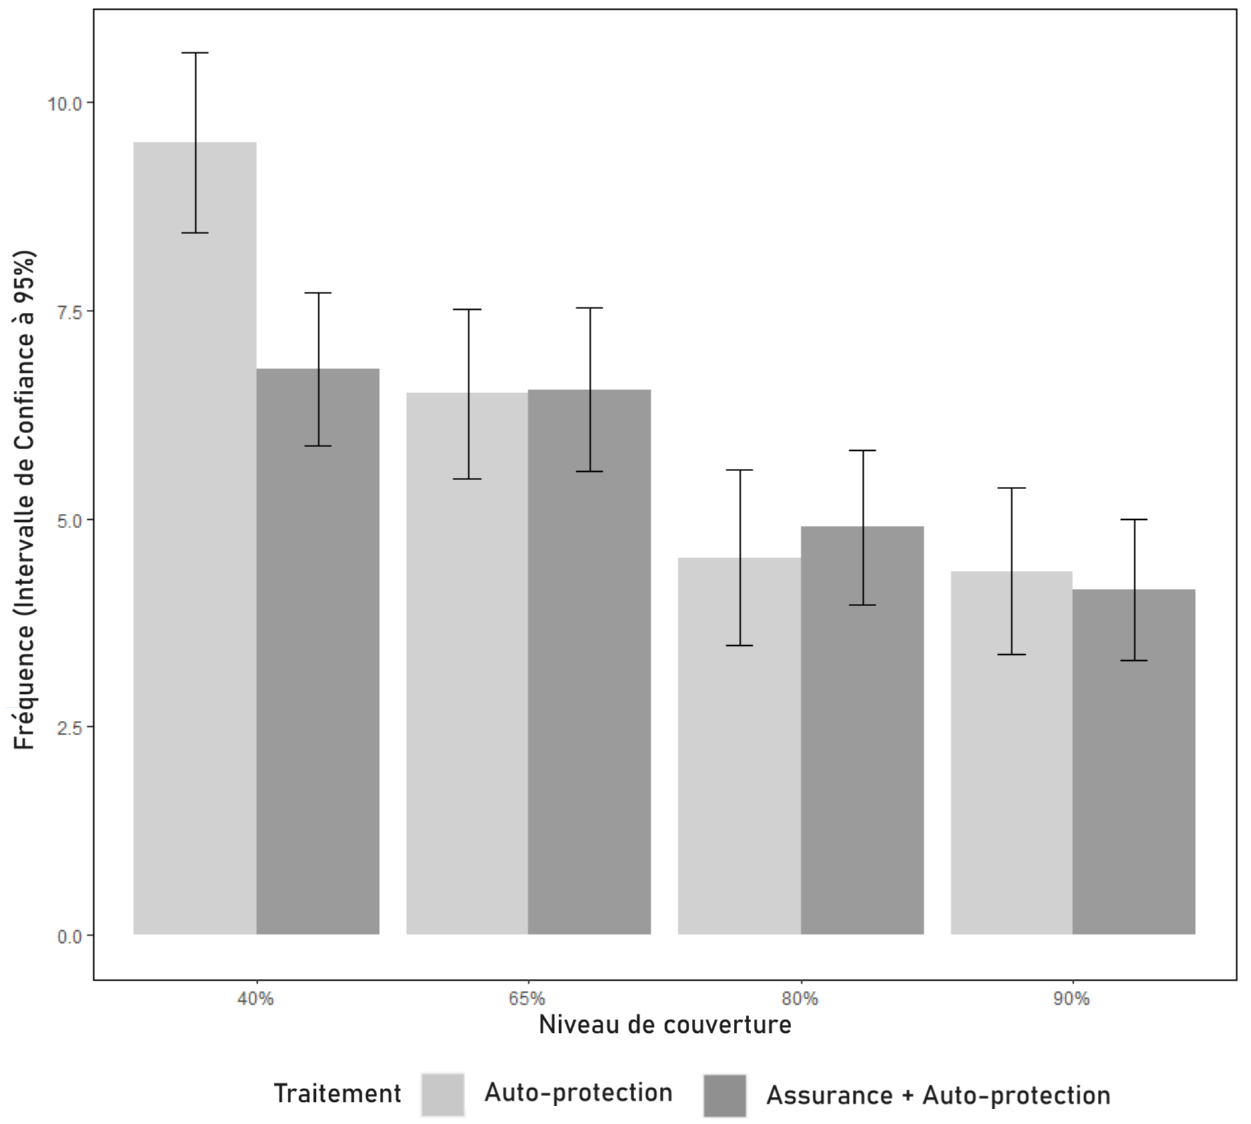
\includegraphics[width=.8\linewidth]{06_insuranceandprevandprev__effort.png}
\end{figure}

À ce stade de l'analyse, un mécanisme de substituabilité entre l'assurance et l'autoprotection semble émerger dans les arbitrages individuels entre ces deux outils de gestion des risques : un plus grand nombre de participants ont choisi des contrats à faible couverture lorsque l'autoprotection était disponible. Ils semblent anticiper leur volonté de réduire la probabilité de perte en utilisant l'autoprotection et décident donc de réduire leur couverture d'assurance dans un premier temps. Ainsi, la décision de réduire la couverture d'assurance dans le traitement \textit{Assurance + autoprotection} pourrait être attribuée à une préférence pour l'autoprotection par rapport à l'assurance, car la disponibilité du mécanisme d'autoprotection est la seule distinction entre les deux traitements.

Afin de confirmer la robustesse de cette hypothèse et, en particulier, de s'assurer que cet effet est bien attribuable à la présence de l'option d'autoprotection et non pas à d'autres paramètres pouvant également influencer les choix d'assurance des individus, trois régressions multivariées ont été estimées. Tout d'abord, un modèle de type logit ordonné à effets aléatoires a été mis en \oe uvre pour estimer le choix d'assurance des participants (modèle 1). Le choix du contrat peut en effet être représenté par une variable catégorielle à quatre modalités, correspondant aux quatre niveaux de couverture disponibles dans chaque menu, avec un ordre sous-jacent (40~\% <~65~\% <~80~\% <~90~\%). Dans ce cadre, le recours à un modèle ordonné à variable latente permet d'identifier l'effet des différents paramètres considérés, y compris la variable de traitement, sur le niveau de couverture choisi par les participants lorsque les choix sont discrets et ordonnés (\textcite{ct05}; \textcite{g11}). Par ailleurs, deux modèles supplémentaires, de type logit à effets aléatoires, ont été effectués pour estimer la probabilité de choisir le contrat avec le taux de couverture le plus bas (40~\%, modèle~2) et le plus élevé (90~\%, modèle 3). Ces deux régressions additionnelles ont été motivées par les résultats descriptifs précédents qui mettent en avant des différences de comportements vis-à-vis des contrats extrêmes et qui sont également les contrats les plus souvent sélectionnés par les participants.

Chacune des trois régressions comprend plusieurs variables de contrôle. Premièrement, deux caractéristiques individuelles ont été incluses : le genre et le niveau d'aversion au risque\footnote{Les variables d'âge et d'éducation ont également été incluses dans les estimations. Compte tenu de la faible variabilité de ces deux variables, les coefficients associés ne ressortent pas significatifs et l'inclusion de ces deux variables n'affecte pas les autres résultats.}. L'aversion au risque est mesurée par le nombre d'options sûres sélectionnées par les participants dans la procédure adaptée du test de \textcite{hl02} au contexte de l'assurance (un participant qui a choisit plus de six options sûres est considéré comme étant averse au risque ; un participant qui choisit huit options sûres est considéré comme plus averse au risque qu'un participant qui en choisit sept)\footnote{Le niveau d'aversion au risque des participants a également été mesuré en considérant le numéro de la question à laquelle ils ont effectué le premier changement d'une option sûre à une option risquée. Les résultats sont similaires puisque 93~\% des sujets sont passés de l'option~A à l'option~B une seule fois ; sur les 7~\% restants, sept sujets ont alternativement choisi les options~A et B (ce qui peut être considéré comme une stratégie de couverture), et un seul participant semble avoir choisi de manière aléatoire (ce participant n'a pas choisi l'option dominante B dans la dernière décision). La majorité de l'échantillon a choisi entre quatre et sept options sûres, ce qui est cohérent avec les résultats trouvés par \textcite{cpm17} en utilisant une procédure similaire.}. Deuxièmement, les caractéristiques de la situation de risque (la probabilité de perte et le montant de la perte) et du menu de contrats d'assurance proposé (le taux de chargement) ont également été prises en compte. Enfin, chaque régression inclut la variable de traitement (\textit{Assurance + autoprotection} \emph{vs} \textit{Assurance}), nécessaire pour estimer l'effet de l'option d'autoprotection sur les choix individuels d'assurance. Le tableau 5 présente les résultats des trois estimations.

% Tableau 5

\begin{table}
  \tabcolsep=2pt
  \caption{Analyses multivariées du choix d'assurance ($\alpha$)}
  \label{tab:insurance_main_results}
  \begin{tabular}[c]{l D{2cm} l D{2cm} l D{2cm} l}
    \toprule
            & \centering Modèle 1 & & \centering Modèle 2 & & \centering Modèle 3 &\tabularnewline
            & \centering Choix d'assurance & & \centering P($\alpha=0,40$) & & \centering P($\alpha=0,90$) &\tabularnewline
    \midrule
    \textbf{\textit{Caractéristiques individuelles}} \\
    \textbf{Genre} \\
    Femme                                & Réf.                             &                         & Réf.                                           &          & Réf.                               &\\
    Homme                                & 0,091 \varstats{0,289}           &                         & 0,784 \varstats{0,356}                         &\sym{**}  & 0,490  \varstats{0,351}            & \\
    \textbf{Aversion au risque}        & 0,118    \varstats{0,099}        &                         & -0,050    \varstats{0,186}                     &          & 0,188    \varstats{0,120}          & \\
    \midrule
    \textit{\textbf{Paramètres du risque}} \\
    \textbf{Probabilité de perte ($\bar{p}$)} \\
    Faible probabilité ($\bar{p}=0,2$)   & Réf.                             &                         & Réf.                                           &          & Réf.                               & \\
    Forte probabilité  ($\bar{p}=0,5$)   & 0,461    \varstats{0,124}        &\sym{***}                & -1,069     \varstats{0,102}                    &\sym{***} & -0,001     \varstats{0,158}        & \\
    \textbf{Montant de perte ($L$)} \\
    Faible perte ($L=600$)               & Réf.                             &                         & Réf.                                           &          & Réf.                               &\\
    Forte perte ($L=1500$)               & 0,645        \varstats{0,124}    &\sym{***}                & -0,546        \varstats{0,100}                 &\sym{***} & 0,648      \varstats{0,160}        &\sym{***}\\
    \midrule
    \textbf{\textit{Caractéristiques du contrat}} \\
    \textbf{Taux de chargement ($\lambda$)} \\
    Nul ($\lambda=0$)                    & Réf.                             &                         & Réf.                                           &          & Réf.                               &\\
    Négatif  ($\lambda=-0,2$)            & 0,331          \varstats{0,151}  &\sym{**}                 & -0,469       \varstats{0,218}                  &\sym{**}  & 0,124       \varstats{0,189}       & \\
    Positif ($\lambda=0,2$)              & -0,424          \varstats{0,150} &\sym{***}                & 0,270      \varstats{0,204}                    &          & -0,715     \varstats{0,199}        &\sym{***}\\
    \midrule
    \textbf{\textit{Traitement}} \\
    \textit{Assurance}                   & Réf.                             &                         & Réf.                                           &          & Réf.                               &\\
    \textit{Assurance + autoprotection} & -0,226        \varstats{0,276}   &                         & 0,715  \varstats{0,330}                        &\sym{**}  & -0,081        \varstats{0,329}     & \\
    \midrule
    Constante                            & -                                &                         & -1,341         \varstats{0,809}                &\sym{*}   & -2,486            \varstats{0,828} &\sym{***}\\
    Seuil 1                              & -0,326        \varstats{0,682}   &                         & -                                              &          & -                                  & \\
    
    Seuil 2                              & 0,831       \varstats{0,682}     &                         & -                                              &          & -                                  & \\
    Seuil 3                              & 1,540         \varstats{0,383}   &\sym{***}                & -                                              &          & -                                  & \\
    \midrule
    \(N\)                                & \multicolumn{2}{c}{960}          & \multicolumn{2}{c}{960} & \multicolumn{2}{c}{960}           \\\bottomrule
    \end{tabular}
    \notedetableau{Significativité : $^{*}$ = 10~\% $^{**}$ = 5~\% $^{***}$ = 1~\%. Les écarts types sont entre parenthèses. Toutes les régressions comprennent des effets aléatoires.}
  \end{table}

  Les résultats révèlent tout d'abord que certaines caractéristiques individuelles, ainsi que celles liées à la situation de risque, affectent les choix d'assurance des participants. Par exemple, même si aucune tendance claire n'est identifiable, le tableau~5 indique une différence entre les choix d'assurance des hommes et des femmes. En particulier, les hommes semblent choisir de moins s'assurer que les femmes, mais avec une différence significative seulement dans la probabilité de sélectionner le contrat avec le taux de couverture le plus bas (modèle~2). De même, conformément à l'intuition qui prévaut en matière de préférence vis-à-vis du risque, un niveau plus important d'aversion au risque semble être associé à des taux de couverture plus élevés (coefficients positifs dans les modèles~1 et 3, et un coefficient négatif dans le modèle~2). Cependant, ce résultat n'est pas statistiquement significatif au seuil de 10~\%. Cette conclusion fait écho à d'autres travaux qui ont montré que le niveau d'aversion au risque joue un rôle limité dans les décisions individuelles d'assurance dans les environnements expérimentaux (\textcite{cpm17}; \textcite{j16}; \textcite{ss11}). Par ailleurs, les caractéristiques du risque ($\bar{p}$ et $L$), ainsi que le taux de chargement ($\lambda$), se révèlent quant à eux des facteurs bien plus déterminants des décisions d'assurance. En particulier, les effets attendus au sens de la théorie économique concernant le montant de la perte et le taux de chargement se retrouvent dans les résultats du tableau 5 : le montant de perte élevé augmente la demande de couverture assurantielle, alors que l'augmentation du taux de chargement tend à la diminuer \parencite{m68}. Enfin, en termes de niveau de risque, alors que les résultats théoriques sont plus ambigus quant à l'effet de la probabilité de perte sur le choix de couverture (\textcite{hr81} ; \textcite{jh95}), la demande d'assurance est plus importante en cas de niveau de risque élevé, dans le cadre de ces données expérimentales.

Concernant spécifiquement l'effet du traitement, il ressort tout d'abord que la présence de l'option d'autoprotection dans le traitement \textit{Assurance + Prévention}, par rapport au traitement \textit{Assurance} dans lequel elle n'est pas proposée, tend à diminuer la probabilité que les individus choisissent un contrat avec un taux de couverture plus important (coefficient négatif dans le modèle~1). Cependant, cet effet n'est pas statistiquement significatif à un seuil de 10~\%. En revanche, une différence significative selon le traitement est observée dans la probabilité de choisir le contrat avec un taux de couverture de 40~\% : l'introduction de l'option d'autoprotection, par rapport au cas où elle n'est pas présente, augmente la probabilité que les participants choisissent le contrat avec le taux de couverture le plus faible (modèle~2), corroborant les résultats descriptifs mis en avant précédemment\footnote{La non-significativité du coefficient associé à la variable de traitement dans le modèle 1 peut s'expliquer par la sur-représentation du taux de couverture de 90\% dans les choix des participants. Cette caractéristique compense l'effet négatif mis en avant dans le modèle~2. De plus, la probabilité de choisir le contrat avec un taux de couverture de 90~\% (modèle~3) est également négative pour les participants du traitement \textit{Assurance + autoprotection} par rapport à ceux du traitement \textit{Autoprotection}, mais non statistiquement significative. À nouveau, la non-significativité de ce coefficient pourrait également être expliquée par le même raisonnement.}.

Ainsi, contrairement à la prédiction théorique (correspondant au résultat attendu principal), les résultats empiriques montrent que l'introduction de l'option d'autoprotection dans le traitement \textit{Assurance + autoprotection} tend à diminuer la demande d'assurance des participants, avec, en particulier, un effet plus marqué sur la probabilité de choisir le contrat avec le taux de couverture le plus faible parmi les options du menu proposé, à autres caractéristiques données. En d'autres termes, lorsque les participants disposent de deux mécanismes de gestion des risques, l'assurance et l'autoprotection, ils vont faire le choix d'acheter moins d'assurance en première étape, par rapport au cas où ils ne disposent que de l'option d'assurance, révélant ainsi un attrait pour l'autoprotection par rapport à l'assurance. Il apparaît donc intéressant de regarder comment cette déviation par rapport à la prédiction théorique, qui ne prévoit pas de changement en matière de choix d'assurance avec ou sans l'option d'autoprotection, se traduit en termes d'effort d'autoprotection. En particulier, est-ce que ce changement de comportement se traduit ensuite par davantage d'efforts d'autoprotection ? Il s'agit ici de tester la cohérence empirique des arbitrages individuels entre l'assurance et l'autoprotection.


\subsection{Incohérence des comportements entre les deux étapes\\ de l'expérimentation}
\label{section:H2selfpro}

Pour analyser et comprendre les décisions individuelles en matière\linebreak d'autoprotection, et surtout examiner si leur choix d'assurance, effectué au préalable, se répercute sur l'effort que les participants consentent à fournir, il est nécessaire de distinguer deux effets : l'effet propre du niveau de couverture (effet de l'aléa moral) et l'effet d'un réel arbitrage individuel entre l'assurance et l'autoprotection. Pour ce faire, un troisième traitement a été mis en \oe uvre, le traitement\textit{ Autoprotection}. Ce traitement, qui consiste à attribuer de manière aléatoire un contrat d'assurance parmi les quatre figurant dans le menu, va permettre d'observer les comportements d'effort d'autoprotection des participants en réaction à la souscription d'un contrat d'assurance donné, afin de capter l'effet propre du niveau de couverture sur le niveau d'effort fourni en seconde étape. Par comparaison avec le traitement \textit{Assurance + autoprotection}, il sera ainsi possible de distinguer l'effet relevant exclusivement du taux de couverture du contrat d'assurance, assimilable à un effet en termes d'aléa moral en cas de diminution de l'effort d'autoprotection avec l'augmentation du taux de couverture attribué, de celui qui relèverait d'une stratégie de diversification entre l'assurance et l'autoprotection comme escompté à partir des résultats précédents (à savoir, est-ce qu'un niveau de couverture plus faible, choisi dans la première étape (résultat précédent), se traduit par un effort d'autoprotection accru dans la deuxième étape ?).

La figure 2 reporte le niveau moyen d'effort d'autoprotection des participants ($e$), en fonction du niveau de couverture assurantielle, selon le traitement (ce taux de couverture est choisi par les participants dans le cas du traitement \textit{Assurance + autoprotection} et imposé dans le cas du traitement \textit{Autoprotection}). Tout d'abord, les niveaux d'effort d'autoprotection observés dans le cadre du traitement \textit{Autoprotection} uniquement, semblent valider l'hypothèse d'un effet d'aléa moral, marqué par une diminution du niveau d'effort avec l'augmentation du taux de couverture imposé aux participants. Par ailleurs, un test non paramétrique de Kolmogorov-Smirnov indique une différence significative globale dans la distribution de $e$ entre les deux traitements (\textit{p-value} = 0,006). Plus précisément, cette différence provient de l'écart significatif d'effort d'autoprotection observé pour le contrat d'assurance disposant du niveau de couverture le plus faible (40~\%). La figure~2 montre clairement que les individus qui ont choisi le contrat avec un taux de couverture de 40~\% (traitement \textit{Assurance + autoprotection}), font en moyenne moins d'effort d'autoprotection que ceux pour qui ce même contrat a été imposé (traitement \textit{Autoprotection}).
 
D’un point de vue théorique, les décisions individuelles en matière d’assurance et d’autoprotection sont indépendantes. Ainsi, aucune différence, en termes de niveau de couverture assurantielle, ne devrait être observée entre les traitements\textit{ Assurance} et \textit{Assurance + autoprotection} ; de même qu’aucune différence ne devrait apparaître entre les traitement \textit{Autoprotection} et \textit{Assurance + autoprotection} en termes d’effort d’autoprotection. Pourtant, les résultats expérimentaux précédents invalident la première prédiction puisqu'une augmentation de la probabilité de sélectionner le contrat le moins complet (40~\%) est observée lorsque l'option d'autoprotection est disponible, par rapport au cas où elle ne l'est pas. Ainsi, si cette régularité empirique s’explique par une préférence pour l’autoprotection par rapport à l’assurance et que les participants restent cohérents dans leur arbitrage entre les deux outils de gestion des risques, des efforts d’autoprotection supérieurs --~bien que contraires aux prédictions théoriques~-- devraient être observés dans le traitement \textit{Assurance + autoprotection}, par rapport au traitement \textit{Autoprotection} (qui pourrait s'interpréter comme  une augmentation compensatrice consécutive à la décision de réduire sa couverture assurarielle). Or, la figure~2 semble contredire cette hypothèse.

% Figure 2

\begin{figure}[h!]
\caption{Niveau moyen d’effort d’autoprotection (e) en fonction du traitement}
  \centering
  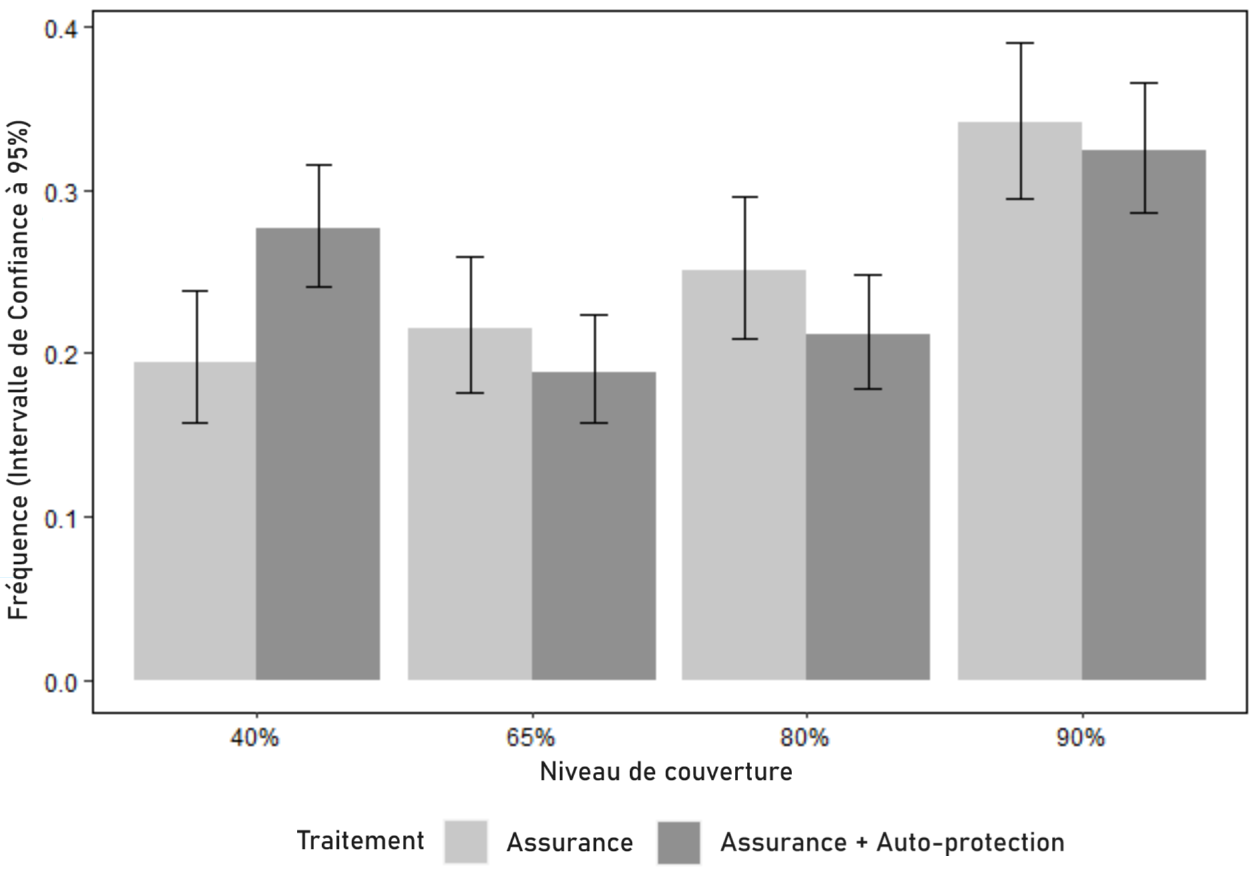
\includegraphics[width=.8\linewidth]{Articles-bons-a-composer/06_Mouminoux_al/06_Mouminoux_Figures/06_distrib_couv_treatment_english.png}
\end{figure}

Pour affiner ces résultats descriptifs, un modèle de régression linéaire à effets aléatoires a été utilisé afin d'estimer le niveau d'effort d'autoprotection $e$ choisi par les participants dans les traitements \textit{Assurance + autoprotection} et \textit{Autoprotection}. La régression inclut, à nouveau, toutes les caractéristiques observables décrites précédemment (caractéristiques individuelles, paramètres du risque et caractéristiques du contrat d'assurance). De plus, trois variables binaires correspondant au niveau de couverture assurantielle dont disposent les participants avant d'effectuer leur effort d'autoprotection --~soit choisi, soit imposé~-- sont également incluses afin de contrôler l'effet propre du taux de couverture sur l'effort d'autoprotection (l'effet de l'aléa moral). Par ailleurs, afin de distinguer l'effet d'aléa moral de celui d'un arbitrage individuel entre l'assurance et l'autoprotection, des termes d'interaction entre chaque niveau de couverture et la variable de traitement ont été ajoutés. Ces variables permettent de tester si la relation entre le niveau de couverture et le niveau d'effort d'autoprotection est la même lorsque le contrat est préalablement choisi par les participants (traitement \textit{Assurance + autoprotection}) ou attribué de manière exogène (traitement \textit{Autoprotection}). Ainsi, si la préférence pour l'autoprotection observée précédemment se traduit par davantage d'efforts d'autoprotection ensuite, un coefficient positif associé au terme d'interaction entre le niveau de couverture à 40~\% et le traitement \textit{Assurance + autoprotection} devrait être observé. Le tableau 6 présente les coefficients estimés.

Tout d'abord, les résultats révèlent une corrélation négative entre le niveau d'assurance et le niveau d'autoprotection, qui se traduit par moins d'efforts d'autoprotection dans le cas de taux de couverture plus élevés, toutes choses étant égales par ailleurs et, en particulier, indépendamment du traitement. En effet, la diminution du taux de couverture, notamment pour les cas des contrats avec les taux de couverture de 40~\% et 65~\%, implique un effort d'autoprotection plus important par rapport au cas des contrats plus complets. Ce premier résultat est conforme à l'hypothèse d'un effet d'aléa moral formulée dans la théorie économique. De même, il est également conforme au résultat obtenu par \textcite{eb72}, dans le cadre d'un modèle à une période, démontrant que l'assurance et l'autoprotection sont des substituts lorsque la prime d'assurance ne prend pas en compte l'effort d'autoprotection.

% Tableau 6

\newpage

\begin{table}[h!]
\caption{Analyses multivariées du niveau d'effort d'autoprotection $e$}
\label{tab:sp_main_results}
\centering
\resizebox{!}{0.45\textheight}{
\begin{tabular}{lrl}
\toprule
   & $e$ & \\
\midrule
\textit{\textbf{Caractéristiques individuelles}} & & \\
\textbf{Genre} & & \\
Femme  & Réf. & \\
Homme  & 1,126 & \\
       & \varstats{0,778} & \\
\textbf{Aversion au risque} & -0,367 & \\
       & \varstats{0,319} & \\
\textit{\textbf{Paramètres du risque}} & & \\
\textbf{Probabilité de perte ($\bar{p}$)} & & \\
Faible probabilité ($\bar{p}=0,2$) & Réf. & \\ 
Forte probabilité ($\bar{p}=0,5$) & 0,646 & \sym{**}  \\
    & \varstats{0,290} & \\
\textbf{Montant de la perte ($L$)} &  &\\
Faible perte ($L=600$) & Réf. & \\
Forte perte ($L=1 500$) & -1,700 & \sym{***} \\
    & \varstats{0,290} & \\
\textit{\textbf{Caractéristiques du contrat}} & & \\
\textbf{Taux de chargement ($\lambda$) } & & \\
Nul ($\lambda=0$)  & Réf. & \\
Négatif ($\lambda=-0,2$) & 0,739 & \sym{**} \\
   & \varstats{0,352} & \\
Positif ($\lambda=0,2$) & 0,748 & \sym{**} \\
   &  \varstats{0,351} & \\
\textbf{Taux de couverture ($\alpha$)} & & \\
40~\% & Réf. & \\
65~\% & -2,609 & \sym{***}\\
     & \varstats{0,588} & \\
80~\% & -3,782 & \sym{***} \\
     & \varstats{0,653} & \\
90~\% & -4,619 & \sym{***} \\
     & \varstats{0,595} &  \\
\textbf{Taux de couverture $\times$ Traitement} \\
40~\% $\times$ Traitement \textit{Assurance + autoprotection} & -1,602 & \sym{*} \\
         &     \varstats{0,909} & \\
65~\% $\times$ Traitement \textit{Assurance + autoprotection} & 0,359 & \\
         &     \varstats{0,934} & \\
80~\% $\times$ Traitement \textit{Assurance + autoprotection} & -0,228 & \\
         &     \varstats{0,953} & \\
90~\% $\times$ Traitement \textit{Assurance + autoprotection} & -0,933 & \\
         &     \varstats{0,889} & \\
\midrule
Constante   &  10,458 & \sym{***} \\
            &  \varstats{2,073} & \\
\(N\)           &  1080 &  \\
\bottomrule
\end{tabular}}
\notedetableau{Significativité : $^{*}$ = 10~\%, $^{**}$ = 5~\%, $^{***}$ = 1~\%. Les écarts types sont entre parenthèses. La régression inclut des effets aléatoires.}
\end{table}

Au-delà de la corrélation négative globale observée entre le niveau de couverture et le niveau d'autoprotection, le résultat central concerne la nature de cette relation en fonction du traitement. En particulier, les résultats montrent que les participants du traitement \textit{Assurance + autoprotection}, qui ont choisi le niveau de couverture de 40~\%, ne fournissent pas un effort d'autoprotection plus important en deuxième étape, par rapport aux participants du traitement \textit{Autoprotection} ($p < 0,10$ associée au terme d'interaction entre le taux de couverture à 40~\% et la variable de traitement). Au contraire, ils fournissent moins d'efforts que les participants à qui ce contrat a été attribué de manière exogène. Pour les autres niveaux de couverture, aucune différence significative dans l'effort d'autoprotection n'est observée selon le groupe de traitement.

Finalement, les participants qui ont choisi d'être moins assurés lors de la première étape dans le traitement \textit{Assurance + autoprotection}, révélant ainsi un attrait pour l'autoprotection, ne fournissent pas plus d'efforts d'autoprotection par la suite (le coefficient négatif suggère même un comportement opposé). Alors que ce résultat est basé sur la comparaison des niveaux d'effort des participants entre les traitements \textit{Assurance + autoprotection} et \textit{Autoprotection}, l'une des interprétations possibles tient à l'existence d'un potentiel effet d'offre lié à l'environnement expérimental du laboratoire \parencite{clv10}. En retirant la possibilité de choisir le contrat d'assurance aux participants dans le traitement \textit{Autoprotection}, faisant ainsi de l'autoprotection le seul outil de gestion du risque manipulable par les participants, ce design pourrait avoir pour effet d’inciter les individus à fournir davantage d’effort d'autoprotection, quel que soit le taux de couverture du contrat attribué (le sujet expérimenté choisirait de faire un effort en raison de sa seule volonté d'apparaître actif lors de l’expérimentation). Pour tester cette hypothèse, il a été question de comparer la probabilité, pour les participants, de ne fournir aucun effort d'autoprotection ($e=0$), entre les deux traitements \textit{Assurance + autoprotection} et \textit{Autoprotection}\footnote{Pour ce faire, un modèle de type logit à effets aléatoires a été utilisé pour estimer la probabilité de ne fournir aucun effort d'autoprotection en fonction du traitement, tout en contrôlant des autres caractéristiques observables.}. Les résultats, reportés dans le tableau~A2 en annexe~\ref{Annexe:supply_effect}, ne semblent pas
valider cette hypothèse puisque la différence dans la probabilité que les participants ne fassent aucun effort ($e = 0$) entre les deux traitements n'est pas statistiquement significative. L’hypothèse d’un  effet d'offre pour expliquer ce résultat est donc peu crédible ici.

En résumé, les résultats ont mis en évidence des comportements individuels différents des prédictions théoriques dictées par la théorie de l'utilité espérée, et marqués par une forme d'incohérence entre deux décisions ayant lieu de manière séquentielle (entre les deux étapes de l'expérimentation). Ce résultat peut être mis en relation avec certains travaux en psychologie sociale, à l'instar de ceux de \textcite{abc04}, qui montrent le rôle majeur du concept de biais hypothétique dans la formation des écarts entre les intentions déclarées des individus et les actions qu'ils entreprennent finalement. Selon l'hypothèse de la présence de biais hypothétiques, l'idée que les individus sont capables de planifier correctement leurs décisions dans un environnement dynamique pourrait être remise en question (la théorie du comportement planifié \parencite{Ajzen1991}). L'expérimentation est conçue de telle sorte que l'effort d'autoprotection n'est qu'hypothétique au moment où les participants choisissent leur contrat d'assurance. En effet, lorsque les deux mécanismes coexistent (traitement \textit{Assurance + autoprotection}), l'étape 1 consiste, pour chaque participant, à choisir un contrat d'assurance sachant que l'autoprotection est disponible ensuite (mais n'apparaît pas encore à l'écran). Le mécanisme d'autoprotection ne devient tangible qu'une fois le contrat souscrit, lors de la seconde étape du jeu (la souscription du contrat d'assurance conduit à l'écran suivant qui affiche l'étape~2). Ainsi, la validation du choix de l'assurance met fin au biais hypothétique et cède la place à l'action d'autoprotection, qui révèle alors la nature de l'incohérence des choix observés. Cette disconnexion entre la préférence et les efforts réellement entrepris a été observée dans plusieurs travaux empiriques. Par exemple, dans le contexte de la santé, \textcite{öjh09} montrent que la volonté des individus à payer pour un traitement médical donné est plus grande que ce qu'ils paient réellement. En utilisant des données expérimentales, \textcite{ms04} analysent les comportements individuels à travers la notion de conformité (ou observance) à un traitement médical et révèlent une différence entre l'acceptation hypothétique et réelle du traitement. \textcite{qtdv18} passent en revue la littérature et mettent en évidence des écarts entre les préférences de santé déclarées (expériences de choix discrets\footnote{Outil économique utilisé pour solliciter les préférences déclarées des répondants.}) et les comportements. Tous ces exemples, qui présentent tous une différence entre les intentions déclarées et les actions entreprises, soulignent l'importance du rôle joué par le biais hypothétique \parencite{hrg15}, et qui pourrait en partie expliquer les résultats expérimentaux obtenus dans cette étude.


\section{Discussion et conclusion}
\label{section:conclusion}

Cette étude repose sur un protocole expérimental ayant pour objectif d'analyser les comportements individuels dans des situations risquées, où l'assurance et l'autoprotection coexistent. À partir de deux traitements expérimentaux différents, les choix individuels en matière d'assurance ont pu être comparés selon que les participants aient, ou non, accès à une option d'autoprotection après avoir souscrit leur contrat d'assurance. Cette première analyse a mis en évidence une relation de substituabilité entre l'assurance et l'autoprotection, marquée par une préférence pour l'autoprotection par rapport à l'assurance. En effet, les individus ont opté pour des contrats moins complets lorsque l'option d'autoprotection était accessible. Par ailleurs, l'implémentation d'un troisième traitement, dans lequel le contrat d'assurance était imposé de façon aléatoire, a ensuite permis d'examiner les efforts d'autoprotection fournis par les individus en deuxième étape et, en particulier, de tester la cohérence des choix séquentiels entre l'assurance et l'autoprotection. Les résultats indiquent que les individus qui semblaient exprimer une préférence pour l'autoprotection à travers leurs choix d'assurance, ne semblent pas fournir davantage d'efforts d'autoprotection une fois rendus à la deuxième étape du jeu. En d'autres termes, l'attrait pour l'autoprotection n'implique pas davantage d'efforts d'autoprotection une fois que le coût de l'effort devient réel.

Ces résultats expérimentaux s'inscrivent dans la continuité des travaux portant sur la question de l'arbitrage entre l'assurance et l'autoprotection. Alors que la plupart de ces travaux ont expliqué la substituabilité entre ces deux outils de gestion des risques par l'effet dissuasif de l'assurance sur l'autoprotection (effet d'aléa moral), cette étude montre que l'introduction d'une option d'autoprotection peut également réduire la demande d'assurance. Dans ce contexte, le développement de contrats d'assurance incluant une option d'autoprotection doit prendre en compte ce résultat pour anticiper d'éventuels comportements de sous-assurance. Cette conclusion est d'autant plus préoccupante compte tenu du deuxième résultat de ce travail, qui révèle que les individus qui semblent exprimer une préférence pour l'autoprotection par rapport à l'assurance ne sont finalement pas enclins à fournir davantage d'efforts d'autoprotection lorsqu'ils sont confrontés au coût réel de cet effort. Ainsi, l'un des principaux défis auxquels les décideurs doivent faire face concerne la motivation à s'engager réellement dans l'autoprotection.

Finalement, bien que l'autoprotection reste souhaitable d'un point de vue global, l'incohérence dans la prise de décisions des individus lorsque plusieurs outils de gestion des risques coexistent soulève de nouvelles questions. Par exemple, comment limiter les effets indésirables et améliorer l'efficacité de l'autoprotection ? \textcite{ArielyWertenbroch2002} soutiennent que la nature auto-contraignante d'une décision pourrait limiter la divergence entre les intentions et les actions, ce qui pourrait être une approche intéressante à adopter. Cependant, contraindre les assurés à s'engager dans l'autoprotection révèle ses propres limites, telles que la nécessité de mettre en place des moyens de contrôle ou encore l'éventualité d'effets d'éviction. Par conséquent, encourager les activités d'autoprotection à travers des campagnes de sensibilisation reste l'un des moyens les plus efficaces de sensibiliser aux risques. Cependant, une attention particulière doit être portée aux comportements de sous-assurance potentiels que les véritables efforts d'autoprotection ne compensent pas.

\printbibliography

\begin{appendices}
  
\section{Instructions}
\label{Annexe:Instruction}

\begin{figure}[htbp]
  \centering
  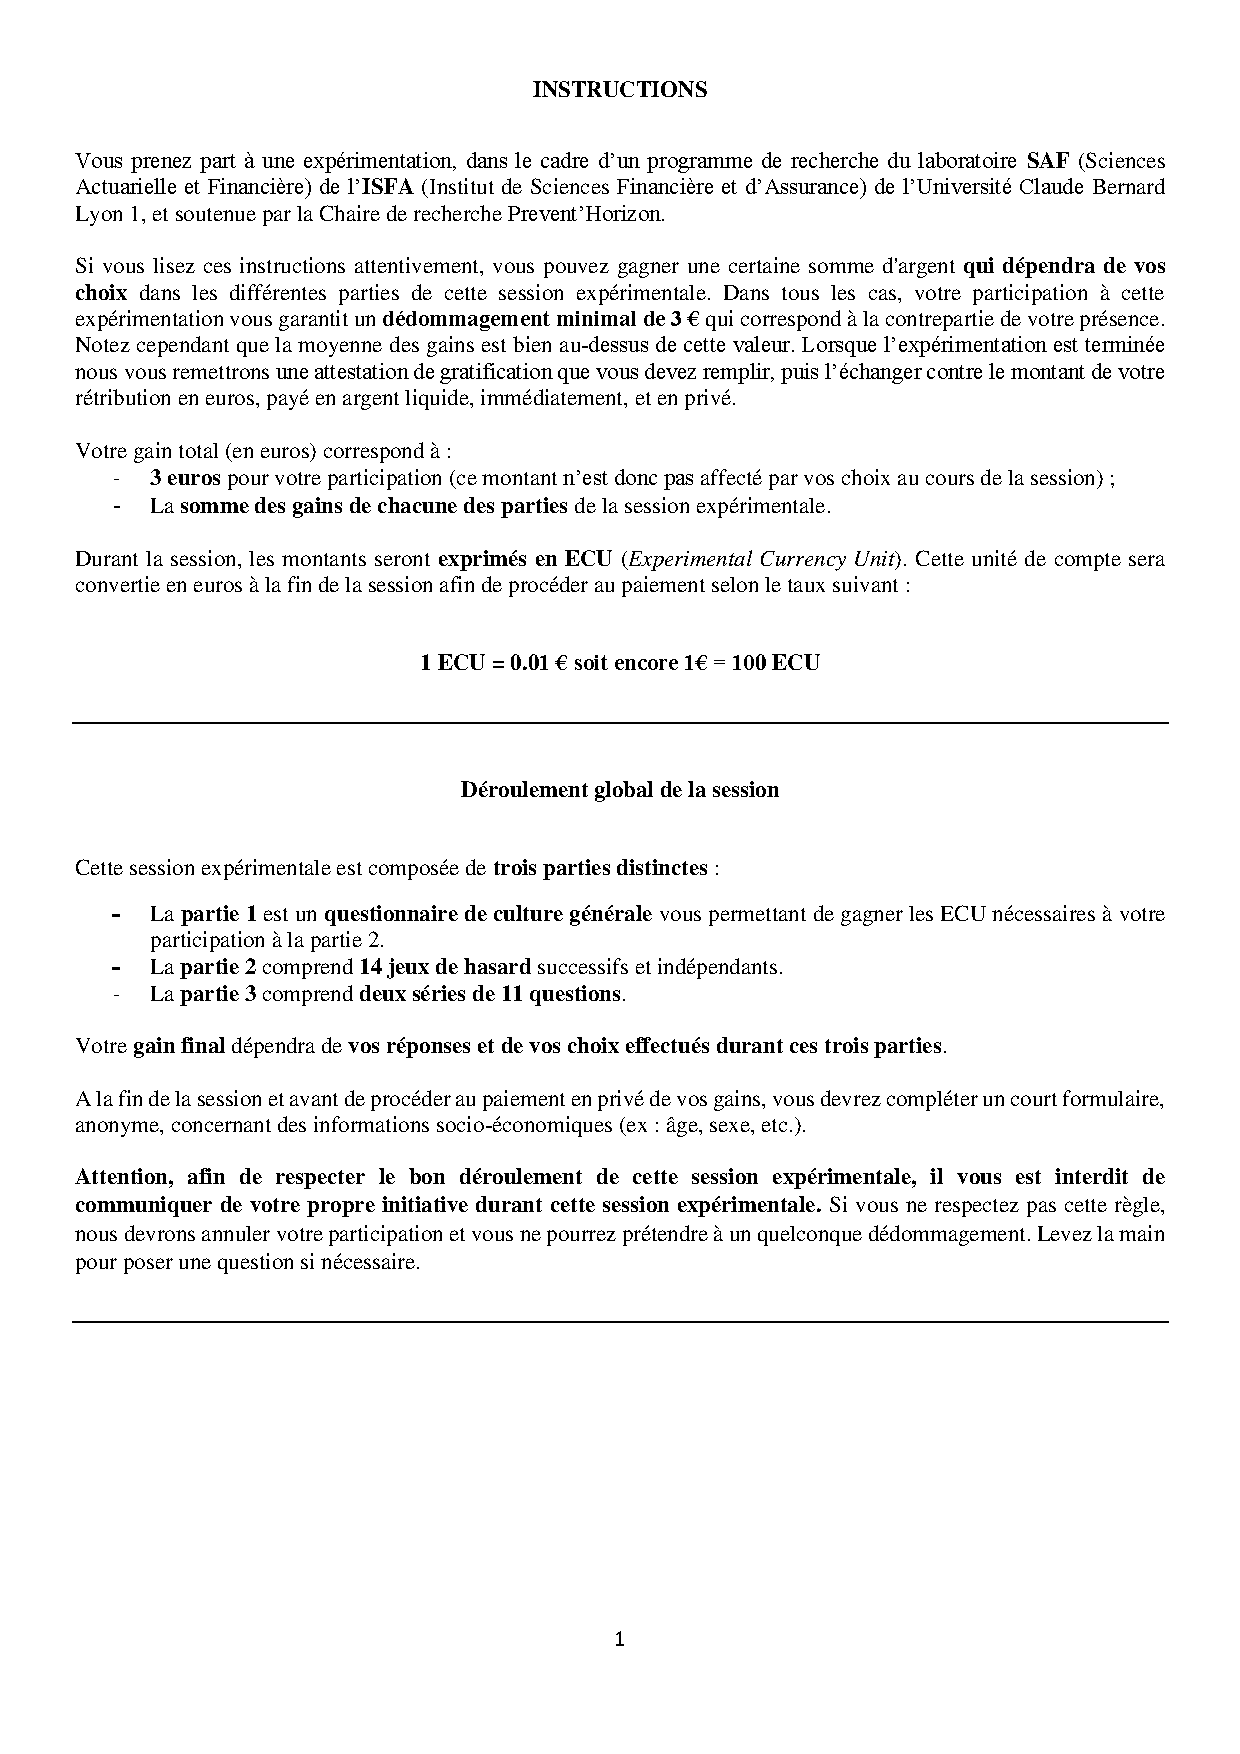
\includegraphics[page=1,scale=0.6]{Articles-bons-a-composer/06_Mouminoux_al/06_Mouminoux_Figures/06_Protocole.pdf}
\end{figure}

\begin{figure}[htbp]
  \centering
  \includegraphics[page=2,scale=0.6]{Articles-bons-a-composer/06_Mouminoux_al/06_Mouminoux_Figures/06_Protocole.pdf}
\end{figure}

\begin{figure}[htbp]
  \centering
  \includegraphics[page=3,scale=0.6]{Articles-bons-a-composer/06_Mouminoux_al/06_Mouminoux_Figures/06_Protocole.pdf}
\end{figure}

\begin{figure}[htbp]
  \centering
  \includegraphics[page=4,scale=0.6]{Articles-bons-a-composer/06_Mouminoux_al/06_Mouminoux_Figures/06_Protocole.pdf}
\end{figure}

\begin{figure}[htbp]
  \centering
  \includegraphics[page=5,scale=0.6]{Articles-bons-a-composer/06_Mouminoux_al/06_Mouminoux_Figures/06_Protocole.pdf}
\end{figure}

\begin{figure}[htbp]
  \centering
  \includegraphics[page=6,scale=0.6]{06_Protocole.pdf}
\end{figure}

\newpage

\section{Résultats attendus}
\label{Annexe:Expected_results}

\subsection{Résultats théoriques}
\label{Annexe:Expected_results_theo}

\paragraph*{Cas 1 : Individus neutres au risque}

Les individus neutres au risque se caractérisent par une fonction d'utilité $U(.)$ linéaire et strictement croissante, et sont supposés maximiser le programme suivant :

\begin{equation}
\left\{
    \begin{array}{ll}
    \displaystyle \max_{\alpha,e} ~~ W - e -\alpha(1+\lambda)\bar{p}L - (\bar{p}-a\cdot e)(1 - \alpha)L\\
    \text{s.c.} ~~0 \le e \le \bar{e}\enskip \text{et}\enskip \underline{\alpha} \le \alpha \le \bar{\alpha}
    \end{array}
\right.
\end{equation}

\noindent avec $\underline{\alpha}$ et $\bar{\alpha}$, respectivement les taux de couverture d'assurance minimum et maximum proposés dans chaque menu de contrats et $\bar{e}$ le niveau d'effort maximum d'autoprotection.

Étant donné que $\alpha$ et $e$ sont des variables de décision prises séquentiellement dans le traitement \textit{Assurance + autoprotection} (choix de $\alpha$ puis de $e$), le recours à un raisonnement par induction récursive (\textit{backward induction}) est nécessaire pour résoudre ce programme d'optimisation. La démarche consiste à déterminer, dans un premier temps, le niveau d'effort d'autoprotection optimal, $e^*(\alpha)$, $\forall\alpha>0$ (étape 1), puis de déterminer le niveau de couverture optimal $\alpha^*$ en fonction de $e^*$, c'est-à-dire en remplaçant $e$ par $e^*(\alpha)$ dans le programme d'optimisation (étape 2). \\

\textit{Étape 1}\footnote{Cette étape correspond également à la résolution du traitement \textit{Autoprotection}.}   \\

Soit $CP=\alpha(1+\lambda)\bar{p}L$ et $D=(1 - \alpha)L$. Ainsi :
\begin{equation}
\left\{
    \begin{array}{ll}
e^* = \arg\max W - e - CP - (\bar{p}-a\cdot e)D = \arg\max e \cdot (aD-1) \\
      \text{s.c.} ~~0 \le e \le \bar{e}
    \end{array}
\right.
\end{equation}

La solution de ce problème d'optimisation consiste à trouver le signe de $(aD-1)$, soit encore le signe de $a(1-\alpha )L-1$, sachant que $D=(1 - \alpha)L$\footnote{En effet, si $(aD-1)=0$ le décideur est indifférent entre les différents niveaux de $e$ (soit $e^*\in [0;\bar{e}]$), si $(aD-1)>0$ alors $e^*=\bar{e}$, et si $(aD-1)<0$ alors $e^*=0$.}.

Sachant que $a=\frac{1}{L}$, étant donné que le coût de l'effort est calculé de sorte que réduire la probabilité de perte à 0 en utilisant l'autoprotection représente le même coût que la souscription d'une assurance complète au prix actuariel, et que l'assurance est obligatoire ($\alpha > 0$), on a :
\begin{equation}
\frac{1}{L}(1-\alpha )L-1=-\alpha<0.
\end{equation}

Ainsi, on obtient $e^*(\alpha)=0,~ \forall \alpha>0$.

\clearpage

\textit{Étape 2} \\

En remplaçant $e$ par $e^*(\alpha)$, on obtient le programme d'optimisation suivant :
\begin{equation}
\left\{
    \begin{array}{ll}
\alpha^* = \arg\max W - CP - \bar{p}D = \arg\max W - \alpha(1+\lambda)\bar{p}L - \bar{p}(1 - \alpha)L \\
\Leftrightarrow \alpha^* = \arg\max ~ -\lambda \alpha \\
    \text{s.c.} ~~\underline{\alpha} \leq \alpha \leq \bar{\alpha}.
    \end{array}
\right.
\end{equation}

Par conséquent, et conformément au modèle de \textcite{m68}, le niveau de couverture optimal pour un individu neutre vis-à-vis du risque dépendra uniquement du signe de $\lambda$, tel que :
\begin{itemize}
  \item Si $\lambda>0$, alors $\alpha^*=\underline{\alpha}$,
  \item Si $\lambda=0$, alors $\alpha^* \in [\underline{\alpha},\bar{\alpha} ]$,
  \item Si $\lambda<0$, alors $\alpha^*=\bar{\alpha} $.
\end{itemize}

\paragraph*{Cas 2 : Individus risquophiles}

Les individus risquophiles se caractérisent par une fonction d'utilité $U(.)$ convexe et strictement croissante, et sont supposés maximiser le programme suivant :
\begin{equation}
\left\{
    \begin{array}{ll}
   \displaystyle \max_{\alpha, e} ~~EU(\alpha,e)=(\bar{p}-a\cdot e)U[W - e -\alpha(1+\lambda)\bar{p}L - (1 - \alpha)L] \\
   + (1 - \bar{p}+a\cdot e)U[W - e - \alpha(1 + \lambda)\bar{p}L] \\
     \text{s.c.} ~~0 \le e \le \bar{e}\enskip \text{et}\enskip \underline{\alpha} \le \alpha \le \bar{\alpha}
    \end{array}
\right.
\end{equation}

\noindent avec $\underline{\alpha}$ et $\bar{\alpha}$, respectivement les taux de couverture d'assurance minimum et maximum proposés dans chaque menu de contrats et $\bar{e}$ le niveau d'effort maximum d'autoprotection.

Le raisonnement par induction récursive est à nouveau utilisé pour déterminer $e^*(\alpha), \forall\alpha>0$ (étape 1), puis $\alpha^*$ (étape 2). \\

\textit{Étape 1} \\

On considère la condition de premier ordre (CPO), soit :
\begin{multline}
\frac{\partial EU(\alpha, e)}{\partial e}=0\Leftrightarrow a(U[W - CP -e] -U[W - CP -D -e]) \\
=(\bar{p}-a\cdot e)U'[W - CP -D -e]+(1 - \bar{p}+a\cdot e)U'[W - CP -e].
\end{multline}

On considère ensuite la condition de second ordre (CSO), soit :
\begin{equation}
\frac{\partial EU(\alpha, e)^2}{\partial e^2}=(\bar{p}-a\cdot e)U''[W - CP -D -e]+(1 - \bar{p}+a\cdot e)U''[W - CP -e].
\end{equation}

Étant donné que $U''(.)>0$, $e^*$ est une solution en coin, telle que $e^* \in \{0;\bar{e}\}$.
Par ailleurs, sachant que $U(.)$ est une fonction strictement croissante et convexe, que la souscription à un contrat d'assurance est obligatoire et que la couverture complète n'est pas disponible ($0<\alpha<1$), en utilisant l'inégalité de Jensen, on a :
\begin{multline}
EU(\alpha, 0)= \bar{p}U[W  -CP - D] + (1 - \bar{p})U[W - CP] \\
> U[\bar{p}\times (W  -CP -D) + (1 - \bar{p}) (W - CP)] = U[W-CP-\bar pD].
\end{multline}

Avec $EU(\alpha, \bar e)=(\bar{p}-a\cdot \bar e)U[W - \bar e -CP - D] + (1 - \bar{p}+a\cdot \bar e)U[W - \bar e - CP],$ soit :
\begin{multline}
EU(\alpha, 0)-EU(\alpha, \bar e) \\
> U[W-CP-\bar pD]-(\bar{p}-a\cdot \bar e)U[W - \bar e -CP - D]- (1 - \bar{p}+a\cdot \bar e)U[W - \bar e - CP] \\
> U[W-CP-\bar pD]-(\bar{p}-a\cdot e)U[W - \bar e -CP - D]- (1 - \bar{p}+a\cdot \bar e)U[W - \bar e - CP-D] \\ 
\Rightarrow EU(\alpha, 0)-EU(\alpha, \bar e) \\
>U[W-CP-\bar pD]-U[W - \bar e -CP - D]>0
\end{multline}

\noindent avec $U(.)$ une fonction strictement croissante et $W-CP-\bar pD>W - \bar e -CP - D \Leftrightarrow \bar e+D>\bar pD \Leftrightarrow e>D(\bar p-1) $ puisque $\bar e>0$, on a donc :
\begin{equation}
EU(\alpha, 0)>EU(\alpha, \bar e),~\forall\alpha~;~ 0<\alpha<1.
\end{equation}

Par conséquent, l'effort optimal d'autoprotection est toujours nul pour les individus risquophiles (soit $e^*(\alpha)=0$) lorsque l'assurance est obligatoire et que la couverture complète n'est pas disponible ($0<\alpha<1$). \\

\textit{Étape 2} \\

La deuxième étape consiste à déterminer $\alpha^*$ sachant $e^*$. Pour ce faire, on considère à nouveau les conditions de premier et second ordre. Soit :
\begin{multline}
\frac{\partial EU(\alpha, e^*)}{\partial \alpha}=0 \\
\Leftrightarrow  (\bar{p}-a\cdot e^*)(-(1+\lambda)\bar{p}L+L)U'[W - e^* -\alpha(1+\lambda)\bar{p}L - (1 - \alpha)L] \\
 + (1 - \bar{p}+a\cdot e^*)(-(1 + \lambda)\bar{p}L)U'[W - e^* - \alpha(1 + \lambda)\bar{p}L]=0.
\end{multline}

Puis :
\begin{multline}
\frac{\partial EU(\alpha, e^*)^2}{\partial \alpha^2}=(\bar{p}-a\cdot e^*)(-(1+\lambda)\bar{p}L+L)^2U''[W - e^* -\alpha(1+\lambda)\bar{p}L - (1 - \alpha)L] \\
+(1 - \bar{p}+a\cdot e^*)(-(1 + \lambda)\bar{p}L)^2U''[W - e^* - \alpha(1 + \lambda)\bar{p}L].
\end{multline}

Sachant que $e^*=0$ et que $U''(.)>0$, cela implique que $\alpha^*$ est également une solution en coin, telle que $\alpha^* \in \{\underline{\alpha};\bar{\alpha}\}$.

En utilisant la CSO et étant donné que $U(.)$ est une fonction strictement croissante ($U'(.)>0$), on peut montrer que pour tout $\lambda \geq 0$, un individu risquophile choisira le taux de couverture le plus faible disponible lorsque l'assurance est obligatoire, soit $\alpha^*=\underline{\alpha}$. En effet, on a :
\begin{multline}
\frac{\partial EU(\alpha, 0)}{\partial \alpha}=-\lambda\bar{p}L[\bar{p}U'[W -CP-D]+(1 - \bar{p})U'[W -CP]] \\
-(1 - \bar{p})U'[W -CP]<0, ~\forall \lambda \geq 0 ,~\forall \overline \alpha >\alpha >\underline \alpha.
\end{multline}

Cependant, puisque le cas où $\lambda<0$ n'est pas exclu (cas d'une assurance subventionnée), un individu modérément risquophile peut avoir un intérêt à choisir la couverture maximale si l'assurance est suffisamment subventionnée.
Dans ce cadre, on a :
\begin{multline}
\frac{\partial EU(\alpha, 0)}{\partial \alpha}=\bar{p}(-(1+\lambda)\bar{p}L+L)U'[W -CP - D] \\
+ (1 - \bar{p})(-(1 + \lambda)\bar{p}L)U'[W - CP] >0, ~\forall \lambda \leq -1 ,~\forall \overline \alpha >\alpha >\underline \alpha. 
\end{multline}

La prime d'assurance est supposée toujours positive, soit $\lambda>-1$. Étant donné que $\frac{\partial EU(\alpha, 0)}{\partial \alpha}<0,~\forall \lambda \geq 0$ et $\frac{\partial EU(\alpha, 0)}{\partial \alpha}>0, ~\forall \lambda \leq -1$, et puisque $\frac{\partial EU(\alpha, 0)}{\partial \alpha}$ est continue en $\lambda$ ; en utilisant le théorème des valeurs intermédiaires, on peut montrer qu'il existe un $\bar{\lambda}$ tel que $0 > \bar{\lambda} > -1$, où $\frac{\partial EU(\alpha, 0)}{\partial \alpha}$ peut être soit positive soit négative en fonction de la valeur de $\alpha$. Ainsi, lorsque $0 > \lambda > -1$, il est nécessaire de comparer l'utilité espérée pour $\alpha^* \in \{\underline{\alpha}, \overline{\alpha}\}$. En particulier, la solution est forcément une solution en coin, qui dépend de la valeur de $\lambda$, avec $\frac{\partial \alpha^*}{\partial \lambda} \le 0$.

\paragraph*{Cas 3 : Individus averses au risque}

Les individus averses au risque se caractérisent par une fonction d'utilité $U(.)$ concave et strictement croissante, et sont supposés maximiser le même programme que celui décrit dans le cas 2 (individus risquophiles). De même, les conditions de premier et second ordre sont les mêmes que celles décrites dans le cas précédent. En revanche, pour le cas des individus averses au risque, on a $U''(.)<0$. Ainsi, la CPO devient suffisante et $e^*$ satisfait la relation suivante : 
\begin{multline}
 a(U[W - CP -e^*] -U[W - CP -D -e^*]) \\
 = (\bar{p}-a\cdot e^*)U'[W - CP -D -e^*] \\
 +(1 - \bar{p}+a\cdot e^*)U'[W - CP -e^*].
\end{multline} 
 
Cependant, il est tout de même nécessaire de vérifier que la solution est une solution intérieure, telle que $e^* \in [0, \overline{e}]$. Si ce n'est pas le cas, étant donné que $e$ prend des valeurs sur un intervalle borné fermé, la solution est une solution en coin.

À ce stade, il est nécessaire de spécifier une forme spécifique de fonction d'utilité, ainsi que des valeurs de paramètres associés, pour obtenir une expression explicite de $e^*$ et $\alpha^*$.


\subsection{Calculs numériques}
\label{Annexe:Expected_results_num}

Bien qu'il soit généralement admis que les individus présentent une aversion absolue au risque décroissante (fonction d'utilité de type DARA), il n'y a pas de consensus parmi les économistes concernant l'aversion relative au risque des individus. \textcite{o14} détaille les différentes conclusions sur l'aversion relative au risque dans la littérature sur la demande d'assurance. Alors que l'utilisation d'une fonction d'utilité avec une aversion au risque relative constante (fonction d'utilité de type CRRA) peut être justifiée selon certaines définitions de la richesse, les individus présentent souvent une aversion relative au risque décroissante (fonction d'utilité de type DRRA), ce qui indique qu'ils deviennent plus tolérants au risque à mesure que leur richesse ou leur niveau de couverture augmente, ce qui peut les amener à opter pour une couverture d'assurance plus faible ou des franchises plus élevées. Ainsi, comme le suggèrent \textcite{hl02}, nous utilisons une fonction d'utilité de type \og\textit{power-expo}\fg, proposée par \textcite{s93}, pour vérifier les résultats précédents dans le cas d'une aversion relative au risque décroissante (fonction d'utilité de type DRRA). Pour ce faire, on considère la fonction d'utilité suivante :
\begin{equation}
U(x) = \theta -e^{-\beta x^\alpha}.
\end{equation}

Les choix théoriques, sous l'hypothèse d'une aversion relative au risque décroissante (fonction d'utilité de type DRRA), sont calculés selon une large gamme de paramètres de la fonction d'utilité, en considérant $\alpha \in [-3,0[$ et $\beta \in [-3,0[$\footnote{$\theta$ est une constante et ne modifie pas les choix lors de la comparaison des loteries selon la théorie de l'utilité espérée.}. Les mêmes résultats précédemment décrits pour l'aversion au risque relative constante (fonction d'utilité de type CRRA) restent valables. De plus, nous constatons que ces résultats sont également valables lorsque l'on considère une aversion relative au risque croissante (fonction d'utilité de type IARA) avec des valeurs de paramètres raisonnables : $0 < \alpha < 1$ et $\beta \in ]0,~3]$, avec $\alpha\beta<0,05$ (par exemple, $\hat{\beta}=0,029$ dans \textcite{hl02}).

\section{Élicitation de l'aversion au risque\\ dans le domaine des pertes}

\label{Annexe:Holt_Laury}

\begin{table}[!h]
    \tabcolsep=3pt
    \centering
\caption{Élicitation de l'aversion au risque}
\label{tab:Holt_Laury}
\begin{tabular}[c]{c|rcrc|c|rcrc|c|r}
\toprule
Décision &\multicolumn{4}{c}{Option A} & E(A)&\multicolumn{4}{c}{Option B} & E(B) & E(A)-E(B)\\
\midrule
1 & 10~\% & -400 & 90~\% & -450 &-445 & 10~\% & -100 & 90~\% & -800 & -820 & 375\\
2 & 20~\% &-400 & 80~\% & -450 & -440 &20~\% & -100 & 80~\% & -800 & -740 & 300\\
3 & 30~\% &-400 & 70~\% & -450 & -435 &30~\% & -100 & 70~\% & -800 & -660 & 225\\
4 & 40~\% &-400 & 60~\% & -450 & -430 & 40~\% & -100 & 60~\% & -800 & -580 & 150\\
5 & 50~\% &-400 & 50~\% & -450 & -425 & 50~\% & -100 & 50~\% & -800 & -500 & 75\\
6 & 60~\% &-400 & 40~\% & -450 & -420 & 60~\% & -100 & 40~\% & -800 & -420 & 0\\
7 & 70~\% &-400 & 30~\% & -450 & -415 & 70~\% & -100 & 30~\% & -800 & -340 & -75\\
8 & 80~\% &-400 & 20~\% & -450 & -410 & 80~\% & -100 & 20~\% & -800 & -260 & -150\\
9 & 90~\% &-400 & 10~\% & -450 & -405 & 90~\% & -100 & 10~\% & -800 & -180 & -225\\
10 & 100~\% &-400 & 0~\% & -450 & -400 & 100~\% & -100 & 0~\% & -800 & -100 & -300\\
\bottomrule
\end{tabular}
\end{table}

\clearpage
\section{Contrôle de l'effet d'offre}
\label{Annexe:supply_effect}


\begin{table}[h!]
\caption{Analyses multivariées de l’effort d’autoprotection $P (e=0)$}
\label{tab:control_supply}
\centering
\resizebox{!}{0.42\textheight}{
\begin{tabular}{lrl}
\toprule
            & $P(e=0)$ & \\
\midrule
\textit{\textbf{Caractéristiques individuelles}} & & \\
\textbf{Genre} & & \\
Femme  & Réf. & \\
Homme            &       -0,167 &          \\
                  &     \varstats{0,417}  &          \\
\textbf{Aversion au risque}     &      0,209   &           \\
                  &    \varstats{0,170}   &      \\
\midrule
\textit{\textbf{Paramètres du risque}} & & \\
\textbf{Probabilité de perte ($\bar{p}$)} & &\\
Faible probabilité ($\bar{p}=0,2$) & Réf. & \\ 
Forte probabilité ($\bar{p}=0,5$)    &     -0,141 & \\
               &    \varstats{0,162}   &     \\
\textbf{Montant de perte ($L$)} & & \\
Faible perte ($L=600$)  & Réf. & \\
Forte perte ($L=1 500$)  &      0,676 & \sym{***}\\
                 &   \varstats{0,164}  &        \\
\midrule
\textit{\textbf{Caractéristiques du contrat}} &  & \\
\textbf{Taux de chargement ($\lambda$) }& & \\
Nul ($\lambda=0$)  & Réf. & \\
Négatif ($\lambda=-0,2$)         &       -0,381 & \sym{**} \\
                  &    \varstats{0,197}      &     \\
Positif ($\lambda=0,2$)       &       -0,351 & \sym{*} \\
                  &   \varstats{0,197}        &       \\
\textbf{Taux de couverture ($\alpha$)} &  & \\
40~\% & Réf. & \\
65~\% &    0,599 & \sym{**}\\
                &    \varstats{0,256} &       \\
80~\%  &      1,185 & \sym{***} \\
                 &    \varstats{0,265} &            \\
90~\%  &       2,271 & \sym{***}      \\
                  &   \varstats{0,257} &    \\
\textbf{Traitement }&  & \\
Traitement \textit{Assurance}  & Réf.  &  \\
Traitement \textit{Assurance + autoprotection} & -0,401 & \\
& \varstats{0,399} & \\
\midrule
Constante     &           -2,777 & \sym{***}\\
                &   \varstats{1,107}  &     \\
\midrule
\(N\)             &        1 080     &     \\
\bottomrule
\end{tabular}}
\notedetableau{Significativité : $^{*}$ = 10~\%, $^{**}$ = 5~\%, $^{***}$ = 1~\%. Les écarts types sont entre parenthèses. La régression inclut des effets aléatoires.}
\end{table}


\end{appendices}

\end{refsection}

\end{Article}
% \begin{Article}[Auteur={Gisèle Umbhauer\thanks{BETA, University of Strasbourg. \emph{Correspondence:} 61 Avenue de la Forêt Noire, 67085 Strasbourg Cedex, France. \emph{E-mail:}\href{mailto:umbhauer@unistra.fr}{\nolinkurl{umbhauer@unistra.fr}}}}, Titre={Minimax Regret in the 11-20 Money Request Game}]

\remerciementsEng{I thank two referees, as well as Jalal El Ouardighi and Bernardo Garcia-Pola for insightful comments. I also thank the third-year class students (year's class 2021/2022) at the Faculté des Sciences Economiques et de Gestion (Faculty of Economic and Management Sciences) of the University of Strasbourg, who played the 11--20 money request game.}

\begin{refsection}[Umbhauer]
\selectlanguage{english}

\begin{resumeENG}
Arad and Rubinstein's 11--20 money request game nicely triggers
level-\emph{k} reasoning. We show, in a general class of money-request games, that mixed-strategy minimax regret plays a significant role too, and that it mimics level-\emph{k} reasoning, at least if the number of level-\emph{k} players in a population is supposed to decrease in \emph{k}. We also show, in this class of games, an original link between the minimax regret probability distribution and the mixed-strategy Nash equilibrium distribution, and we compare the payoffs obtained with both concepts.
\end{resumeENG}

\titrearticleENG{Minimax regret et jeu de demande 11-20}

\begin{resume}
Le jeu de demande 11-20 d'Arad et Rubinstein stimule naturellement un comportement conforme au raisonnement de niveau-\emph{k}. Nous montrons, dans une version généralisée de ce jeu, que le minimax regret joue également un rôle significatif dans le comportement induit et que la stratégie mixte de minimax regret mime le raisonnement de niveau-\emph{k}, dès lors que le nombre de joueurs de niveau-\emph{k} dans une population chute avec \emph{k}. Nous montrons également qu'il existe, pour cette famille de jeux, un lien original entre la stratégie mixte de minimax regret et l'équilibre de Nash en stratégies mixtes, et nous comparons les paiements obtenus avec les deux concepts.
\end{resume}

\keywords{mixed minimax regret, level-\emph{k} reasoning, money-request game, Nash equilibrium}

\motscles{minimax regret en stratégies mixtes, raisonnement de niveau-\emph{k}, jeu de demande 11-20, équilibre de Nash}

\jelcode{C72}


\section{Introduction}

\textcite{arad2012} presented the 11--20 money request game
as the game that naturally triggers level-\emph{k} reasoning. In this
2-player game, each player requests an amount of money. This amount is an integer between 11 and 20. Each player receives the amount he asks for. And a player gets an additional amount of 20 if he requests exactly one unit less than the other player.

Arad and Rubinstein (AR henceforth) are partly right in claiming that
this game is well suited for studying level-\emph{k} reasoning. First, everything is done in this game to stimulate level-\emph{k} reasoning. The level-0 behavior seems to find consensus: by playing 20, a player is sure to get 20, which is a very large (unusual) maximin payoff. Hence a player who does not want to engage in iterative reasoning will surely request 20, so 20 is the natural starting point for the level-\emph{k} iterations. It follows that playing 19 is the natural level-1 behavior (because 19 is the best response to 20), that 18 is the natural level-2 behavior (because 18 is the best response to 19), and so on. Conflict between the two players is circumscribed in that each player gets the amount he asks for, regardless of what is played by the opponent, so individual optimization should not be limited by social considerations.

Second, the sequence of level-\emph{k} iterations cannot be obtained by other common ways of reasoning. There is no dominated strategy in the 11--20 money request game, so iterative dominance has no bite and cannot lead to the same outcome as level-\emph{k} behavior (by contrast to what happens in the guessing game (beauty contest), see \textcite{nagel1995}). There is also no pure strategy Nash equilibrium that is the limit behavior of level-\emph{k} reasoning (by contrast to the guessing game). Third, the game is very easy and requires few (almost no) cognitive skills to progress in the level-\emph{k} process. By contrast to guessing games where each additional step requires calculating a new mean, here each additional step consists just in decreasing the requested amount by 1; this fact explains why a slightly simplified version of Arad and Rubinstein's game (AR's game henceforth) has been used in experiments with very young children, from five years old (see \textcite{fe2022}). For all these reasons, the 11--20 money request game seems to be a good game to test level-\emph{k} reasoning, and especially the depth of reasoning (number of iterations performed by the players).

This game has given rise to many experiments (among them \textcite{arad2012}, \textcite{lindner2013}, \textcite{goeree2018}, \textcite{li2018}, \textcite{alosferrer2021}). Some of these studies have brought insights into time and depth of reasoning. \textcite{lindner2013} studied whether time pressure was able to stimulate a behavior closer to the mixed strategy Nash equilibrium, whereas \textcite{alosferrer2021} studied the link between deliberation times and depth of reasoning.

Yet AR's game has a property not shared by other level-\emph{k} testing
games like the usual guessing game. As observed by \textcite{li2018}, in contrast to the guessing game where the players always
get the same amount (1 for the winner and 0 for the losers), the payoff
obtained by a player in the money request game strongly depends on the
chosen number. The maximal and minimal amounts a player can win with a
given integer are increasing in the number played (except for 20): a
player gets at least 19 and at most 39 by playing 19 but only at least
11 and at most 31 by playing 11. This fact may trigger behavioral traits
that are different from level-\emph{k} reasoning. \textcite{li2018}
mention risk aversion, which indeed leads to players playing large
numbers more frequently, while \textcite{goeree2018} show that common
knowledge of noise in behavior also leads to large numbers being played
more often.

In this paper, we argue that minimax regret is another way to approach
the game. Minimax regret (MR henceforth) is well known in decision
theory, where it is associated with ambiguity aversion---and goes back
to \textcite{savage1951} and \textcite{niehans1948}---but it has only more
recently been introduced into game theory, notably by \textcite{linhart1989}, \textcite{renou2010} and \textcite{halpern2012}. As a matter of fact, the 11--20 money request game exhibits a strong strategic uncertainty: according to \textcolor{red}{Pearce's concept [1984]}, each amount is rationalizable (because each request \emph{x}
from 11 to 19 is the best response to the request \(x + 1\), and 20 is
the best response to the request 11). So it is difficult to anticipate
the other's behavior and each decision may generate a regret. It follows
that it may be more reasonable to minimize the generated regrets rather
than trying to best respond to a strategy that cannot be anticipated.
And it turns out that the mixed MR strategy corresponds to the outcome
distribution observed with level-\emph{k} players, up to a certain depth
of reasoning, provided one assumes that the number of players in a
population is decreasing in the depth of reasoning. So level-\emph{k}
behavior can also be obtained by regret minimization despite its
conveying a completely different philosophy. \textcite{garciapola2020} already observed a link between level-1 reasoning and iterative pure-strategy MR. But pure-strategy MR only focuses on maximal regrets, which is very restrictive. Mixed-strategy MR better exploits all the regrets in the game and leads to a more interesting link between MR and level-\emph{k} reasoning.

The aim of this paper is to investigate the link between mixed-strategy
MR and level-\emph{k} reasoning, as well as the link between
mixed-strategy MR and the mixed-strategy Nash equilibrium in a general
version of the 11--20 money request game. We also compare the payoffs
obtained with MR and the Nash equilibrium. Finally we show how MR
behaves in variants of the 11--20 money request game developed by \textcite{arad2012} and \textcite{goeree2018}, and we make some behavioral
comments drawing on a classroom experiment.

In section~\ref{section:The 11-20 money} we start by briefly showing how 410 students played the 11--20 money request game in a classroom experiment at Strasbourg
university. This classroom experiment will be used to illustrate the
results set out in the following sections. In section~\ref{section:Minimax regret in the money} we establish the mixed-strategy MR regret behavior in the 11--20 money request game, before looking for this behavior in a general money request game. We
show that the mixed MR strategy mimics an outcome distribution of
level-\emph{k} players, if the percentage of players is decreasing in
the depth of reasoning. In section~\ref{section:Minimax regret, Nash equil} we study the original link between the mixed MR strategy and the mixed-strategy Nash equilibrium in the money request games, and we discuss the payoffs obtained with both
concepts. Section~\ref{section:Comments on minimax regrets} investigates the impact of MR in some variants of AR's game. Section~\ref{section:Conclusion_Umbhauer_en} concludes with behavioral comments drawing on the classroom experiment in Strasbourg.


\section[The 11-20 money request game, a classroom experiment]{The 11-20 money request game,\\ a classroom experiment}
% entre crochets le titre tel qu'il serait imprimé en table des matières ou en tête de page si c'était le cas
% entre accolades, le titre tel qu'on veut l'afficher dans le corps du texte
\label{section:The 11-20 money}

The classroom experiment was run during a third-year class in game
theory at the faculty of economics and management of the University of
Strasbourg in the academic year 2021--2022. In total 410 students
participated in the experiment. Subjects were homogeneous in age (almost
all students were 19--21~years old) and field of study (economics and
management). As is common in classroom experiments, no monetary rewards
were used to incentivize subjects but students were told that they could
obtain a bonus in the final grade for their participation in the
experiment. The experiment is a one-shot AR's game. The game was
explained and several examples were given to the students before the
beginning of the experiment, to be sure that the rules of the game were
understood.\footnote{To facilitate the understanding of the game we
  talked about amounts in euros (in \textcite{arad2012} the amounts are in
  shekels).} The students played the game before knowing the concepts of
dominance and Nash equilibrium (NE), but they knew the notion of a
normal form matrix game. So, when taking their decision, they had in
front of them the normal form matrix of the 11--20 money request game
(matrix 1).\footnote{To facilitate the reading of the matrix, player 1's
  payoffs were written in red. In the other experiments with the 11--20
  money request game, the players usually do not have the payoff matrix
  in front of them. Yet having the matrix at one's disposal may have an
  impact on the choices in that it facilitates the comparison of one's
  own payoff with the payoff of the opponent (we come back to this fact
  in section~\ref{section:Conclusion_Umbhauer_en}).}

\begin{table}[h!]
\centering
Matrix 1: The 11-20 money request game with bonus~20
\label{matx1}
\resizebox{.90\linewidth}{!}{
\begin{tabular}{lc | c*{9}{c} | }
\multicolumn{12}{c}{P12} \tabularnewline % fusionner 12 cellules, centrer (c)
 & \multicolumn{1}{c}{} & 11 & 12 & 13 & 14 & 15 & 16 & 17 & 18 & 19 & \multicolumn{1}{c}{20} \tabularnewline
\cline{3-12}
& 11 & (11,11) & (31,12) & (11,13) & (11,14) & (11,15) & (11,16) &
(11,17) & (11,18) & (11,19) & (11,20) \tabularnewline
& 12 & (12,31) & (12,12) & (32,13) & (12,14) & (12,15) & (12,16) &
(12,17) & (12,18) & (12,19) & (12,20) \tabularnewline
& 13 & (13,11) & (13,32) & (13,13) & (33,14) & (13,15) & (13,16) &
(13,17) & (13,18) & (13,19) & (13,20) \tabularnewline
& 14 & (14,11) & (14,12) & (14,33) & (14,14) & (34,15) & (14,16) &
(14,17) & (14,18) & (14,19) & (14,20) \tabularnewline
Pl1 & 15 & (15,11) & (15,12) & (15,13) & (15,34) & (15,15) & (35,16) &
(15,17) & (15,18) & (15,19) & (15,20) \tabularnewline
& 16 & (16,11) & (16,12) & (16,13) & (16,14) & (16,35) & (16,16) &
(36,17) & (16,18) & (16,19) & (16,20) \tabularnewline
& 17 & (17,11) & (17,12) & (17,13) & (17,14) & (17,15) & (17,36) &
(17,17) & (37,18) & (17,19) & (17,20) \tabularnewline
& 18 & (18,11) & (18,12) & (18,13) & (18,14) & (18,15) & (18,16) &
(18,37) & (18,18) & (38,19) & (18,20) \tabularnewline
& 19 & (19,11) & (19,12) & (19,13) & (19,14) & (19,15) & (19,16) &
(19,17) & (19,38) & (19,19) & (39,20) \tabularnewline
& 20 & (20,11) & (20,12) & (20,13) & (20,14) & (20,15) & (20,16) &
(20,17) & (20,18) & (20,39) & (20,20) \tabularnewline
\cline{3-12}
\end{tabular}}
\end{table}

  
The students had to answer the following question: ``Imagine you
are player~1 and you are confronted with another student, player~2,
randomly selected from all the other students. What amount do you ask
for?'' The students were invited to justify their choices in writing.
The results are given in table 1 and represented in figure 1. Table 1
also gives the results obtained in the experiments by AR {[}2012{]} and \textcite{li2018} (LR henceforth), as well as the mixed-strategy
symmetric NE,\footnote{The 11--20 money request game has other
  asymmetric mixed-strategy Nash equilibria, but they all meet the
  property that the probabilities on the played actions decrease in the
  played numbers, with a possible exception for the lowest played
  number. One of these equilibria is such that one player plays 13, 15,
  17, 19, respectively with the probabilities 8/20, 6/20, 4/20 and 2/20,
  whereas the other plays 12, 14, 16, 18 and 20, respectively with the
  probabilities 2/20, 7.5/20, 5.5/20, 3.5/20 and 1.5/20.} and the mixed
MR strategy we turn to in section~\ref{section:Minimax regret in the money}.

\begin{table}[h!]
\caption{Some experiments on the 11--20 money request game with
bonus 20, as well as the symmetric mixed Nash equilibrium and the mixed
minimax regret strategy}\label{tab1}
\centering
\resizebox{\linewidth}{!}{
\begin{tabular}{l    *{10}{D{6mm}}}
\toprule
Requested amount & \centering 11 & \centering 12 & \centering 13 & \centering 14 & \centering 15 & \centering 16 & \centering 17 & \centering 18 & \centering 19 & \centering 20 \tabularnewline
\midrule
Strasbourg's experiment (\%) & 8.3 & 0.7 & 2 & 4.4 & 4.9 & 5.9 & 14.9 &
17.5 & 28 & 13.4 \tabularnewline
AR's experiment (\%) & 4 & 0 & 3 & 6 & 1 & 6 & 32 & 30 & 12 & 6 \tabularnewline
LR's experiment (\%) & 0 & 0 & 0 & 7.3 & 1 & 4.2 & 19.8 & 37.5 & 26 &
4.2 \tabularnewline
Symmetric NE (\%) & 0 & 0 & 0 & 0 & 25 & 25 & 20 & 15 & 10 & 5 \tabularnewline
Mixed MR strategy (\%) & 0 & 0 & 0 & 0 & 5 & 10 & 15 & 20 & 25 & 25 \tabularnewline
\bottomrule
\end{tabular}}
\end{table}


\begin{figure}[h]
    \centering
    \caption{Strasbourg University's classroom experiment (percentages) (2021/2022)}
    \includegraphics[height=7cm]{Articles-bons-a-composer/07_Umbhauer_en/07_Umbhauer_en_figures/Umbhauer_fig1.jpeg}
\end{figure}


Figure 1 is in line with a common observation made in many games
triggering level-\emph{k} behavior, namely guessing games (beauty
contests), according to which the number of players engaging in
level-\emph{k} reasoning is decreasing in the depth of reasoning
(\(k > 0\)). So 28\% of the students in Strasbourg choose 19 (level-1
reasoning), 17.5\% of them play 18 (level-2 reasoning), 14.9\% of them
play 17 (level-3 reasoning) and so on, down to 12 (see table 1). Only
the fact that 8.3\% of the students play 11 is not in accordance with
this fact. This smooth decreasing relationship from 19 to 12 is not
always obtained in other experiments on the 11--20 money request game.
19 is not always the statistical mode of the behavior distribution: 19
is the statistical mode in \textcolor{red}{Alos-Ferrer and Buckenmaier [2018]}, 17 is
the statistical mode in AR {[}2012{]}, and 18 is the statistical mode in \textcite{goeree2018}, \textcite{li2018} and \textcite{lindner2013}. More generally, the behavior distributions vary among the studies,\footnote{For example, a chi-square test on the populations, even if restricted to the distributions on the range 16--19, shows that AR's distribution (108 players) is statistically significantly different from the distribution obtained in the Strasbourg classroom experiment (410 players) (\emph{p}-value~<~0.001). Strasbourg's
  distribution is closer to the one obtained in \textcolor{red}{Alos-Ferrer and  Buckenmaier {[}2018{]}} (128 players), except for the number of players
  playing 17, which is quite low in Alos-Ferrer and Buckenmaier: both
  distributions, when restricted on the numbers 16, 18, 19 and 20, are
  not statistically significantly different (\(p = 0.14\)).} but all the
experiments share the property that the percentages decrease from 18 (17
for AR) to at least 14 (in any case, the percentages of players choosing
11, 12, 13 are generally small). And all the empirical distributions are
markedly different from the symmetric NE (the \emph{p}-value of the
chi-square tests can be approximated by 0).

\section{Minimax regret in the money request games}
\label{section:Minimax regret in the money}

We now turn to MR and apply this concept to a generalized version of
AR's game, the 11--\emph{T} money request game with bonus \emph{B}, with
\(B \geq T > 11 + n\), where \emph{n} is the integer defined by:
\(n(n + 1)/2\  \leq B < (n + 1)(n + 2)/2\) (\(B = T = 20\) and \(n = 5\)
in AR's game).

The notion of MR is well known in decision theory with uncertainty,
going back to \textcite{savage1951} and \textcite{niehans1948}. An economic
agent who is unable to anticipate a future state of the world (state of
Nature) may opt for a strategy that minimizes his regret, which is the
difference between the payoff obtained with his decision and the payoff
obtained with the best decision in the realized state of the world. MR
can partly explain the behavior of the agents in Ellsberg's paradox
\parencite{ellsberg1961}. In a game, players are not confronted with Nature or
lotteries---at least not exclusively---but with other players. Yet they
may also suffer from a strong strategic uncertainty, in that it may be
difficult, for many reasons, to anticipate how the other players will
play. In such a context, minimizing regrets may be more optimal than
best-replying to a completely unknown profile of strategies.

In a game, the pure-strategy MR concept goes as follows: in a
normal-form game with \emph{N} players \emph{i}, pure strategy sets
\emph{S\textsubscript{i}} and utility functions
\emph{u\textsubscript{i}}, with \emph{i} from 1 to \emph{N}, player
\emph{i}'s regret by playing the pure strategy \(s_{i}\ \)when the
opponents play the pure strategies \(s_{- i}\) is
\(r_{i}(s_{i}, s_{- i}) = \max_{\sigma_{i} \in S_{i}}{u_{i}\left( \sigma_{i}, s_{- i} \right) - u_{i}\left( s_{i}, s_{- i} \right)}\).
The maximal regret \emph{s\textsubscript{i}} leads to is
\(R_{i}\left( s_{i} \right) = \max_{s_{- i} \in S_{- i}}{r_{i}(s_{i}, s_{- i})}\).
Player \emph{i}'s pure-strategy MR is
\(\min_{s_{i} \in S_{i}}{R_{i}\left( s_{i} \right)}\) (see \textcite{linhart1989}, \textcite{halpern2012} and \textcite{renou2010} for more details).

Hence the regret generated by a chosen strategy, given an opponent's
strategy, is the difference between the payoff obtained with the
best-reply to the opponent's strategy and the payoff obtained with the
chosen strategy. For example, in the 11--20 money request game, if
player 1 asks for 14 whereas player 2 asks for 17, player 1's best
response is 16, and so player~1's regret, \emph{r}(14,17), is
$36-14=22$. The maximal regret the amount 14 may lead to,
\emph{R}(14), is obtained when player~2 chooses 20, in which case the
best response is 19 and the maximal regret generated by 14 is $39-14=25$.

The regret matrix for player 1 in AR's game is matrix 2. The maximal
regret assigned to each amount \emph{m}, \(R(m),\ m\) from 11 to 20, is
in bold in the matrix.

This matrix sheds light on the characteristics of the regrets. The
regrets in italics, equal to 19, express the fact that if both players
request \emph{x}, each player regrets not requesting \(x - 1\): he would
receive the additional amount \(B - 1\) by doing so (\emph{B} being the
bonus equal to 20 in AR's game). The regrets in the last column are the
regrets a player suffers when he plays \emph{x} different from 19 and
the opponent plays 20. The lower the requested amount \emph{x}, the more
he suffers, because he suffers both from the loss of the bonus 20 and
from the difference \(19 - x\).

\begin{table}[h!]
\centering
Matrix 2: Player 1's regret matrix in the 11--20 money request game\\ with bonus~20 \par
\vspace{0.2cm}
\label{matx2}
\resizebox{.55\linewidth}{!}{
\begin{tabular}{lc | c*{9}{c} | }
\multicolumn{12}{c}{P12} \tabularnewline
& \multicolumn{1}{l}{} & 11 & 12 & 13 & 14 & 15 & 16 & 17 & 18 & 19 & \multicolumn{1}{l}{20} \tabularnewline
\cline{3-12}
& 11 & 9 & 0 & 21 & 22 & 23 & 24 & 25 & 26 & 27 & \textbf{28} \tabularnewline
& 12 & 8 & \emph{19} & 0 & 21 & 22 & 23 & 24 & 25 & 26 & \textbf{27} \tabularnewline
& 13 & 7 & 18 & \emph{19} & 0 & 21 & 22 & 23 & 24 & 25 & \textbf{26} \tabularnewline
& 14 & 6 & 17 & 18 & \emph{19} & 0 & 21 & \emph{22} & 23 & 24 & \emph{\textbf{25}} \tabularnewline
Pl1 & 15 & 5 & 16 & 17 & 18 & 19 & 0 & 21 & 22 & 23 & \textbf{24} \tabularnewline
& 16 & 4 & 15 & 16 & 17 & 18 & \emph{19} & 0 & 21 & 22 & \textbf{23} \tabularnewline
& 17 & \ul{3} & \ul{14} & \ul{15} & \ul{16} & \ul{17} & \ul{18} &
\emph{\ul{19}} & \ul{0} & \ul{21} & \textbf{\ul{22}} \tabularnewline
& 18 & \ul{2} & \ul{13} & \ul{14} & \ul{15} & \ul{16} & \ul{17} &
\ul{18} & \emph{\ul{19}} & \ul{0} & \textbf{\ul{21}} \tabularnewline
& 19 & 1 & 12 & 13 & 14 & 15 & 16 & 17 & 18 & \emph{\textbf{19}} & 0 \tabularnewline
& 20 & 0 & 11 & 12 & 13 & 14 & 15 & 16 & 17 & 18 & \emph{\textbf{19}}
\tabularnewline
\cline{3-12}
\end{tabular}}
\end{table}


The matrix is quite regular in structure. On line \emph{x} (the amount
requested by player 1) the regrets are increasing in the opponent's
(player 2) amount \emph{y} up to \(y = x\), and they increase again in
player 2's amount \emph{y} from \(y = x + 2\) to \(y = 20\). Except for
\(x = 19,\) the maximal regret \(R(x)\) is always obtained in the last
column, when the opponent plays 20. This is due to the fact that the
regret in this column, except for 0, is \(B + 19 - x,\) whereas in
column \emph{y}, with \(11 < y < 20\), it is \(B + y - 1 - x\), which is
lower by construction.

\textcite{garciapola2020} observed that the pure-strategy MR in this game,
equal to 19, is obtained for \(x = 19\) and \(x = 20\), and that
applying the pure-strategy MR concept in an iterative way \parencite{halpern2012} leads to 19. By comparing MR with level-\emph{k} reasoning,
he concluded that, in this game, MR and level-1 reasoning lead to
requesting the same amount, 19.

In this paper we go further by turning to mixed-strategy MR, a concept
that takes into account all the regrets in matrix 2 (and not only the
maximal---bold--- regrets). We call \emph{x}, respectively \emph{y}, the
amounts played by player 1, respectively player 2 (the opponent). The
regrets in any line \emph{x} are regularly increasing in the opponent's
amount \emph{y} because they are equal to \(y - 1 + B - x\ \)(except for
\(y = x + 1\)). Comparing adjacent lines \emph{x} and \(x + 1\) (for
example the underlined lines 17 and 18) leads us to observe that player
1's regrets are always lower in line \(x + 1\) than in line \emph{x},
except if the other player plays \(x + 1\) (in this case, player 1's
regret is null when he plays \emph{x} and equal to 19 when he plays
\(x + 1\)). This fact expresses that a player regrets the unit of money
he deliberately and systematically loses when he plays \emph{x} instead
of \(x + 1\), except if the other player fortunately plays \(x + 1\).
Similar observations can be made by comparing two adjacent columns,
\emph{y} and \(y + 1\) (for example the squared columns 17 and 18). This
time the regrets are systematically one unit larger in column \(y + 1\)
than in column \emph{y}, because they switch from \(B + y - 1 - x\) to
\(B + y - x\). The regrets in column \emph{y}, i.e. when the opponent
plays \emph{y}, are regularly decreasing in \emph{x} (except for
\(x = y - 1\)). This follows from the fact that the regret
\(B + y - 1 - x\ \)can be split into two parts: the regret player 1
suffers when he plays 20, \(y - 1 + B - 20\), plus the regret he suffers
because he does not play 20, \(20 - x\), except for \(x = y - 1\). So
the regrets in column \emph{y} are decreasing in \emph{x} because
\(20 - x\) is decreasing in \emph{x}.

This intuitively leads to the following expectation: a concept of regret
should assign a stronger probability to larger numbers. This expectation
is revealed to be correct.

We work with \textcite{renou2010} mixed notion of regret. The
idea is to construct a mixed strategy that minimizes the regret, called
\emph{z}, regardless of the amount requested by the opponent. We call
\emph{p\textsubscript{t}} player 1's probability of requesting \emph{t}.
This amounts to solving the optimization program:
%
\[
\min_{z\ p_{11}p_{12}p_{13}p_{14}p_{15}p_{16}p_{17}p_{18}p_{19}p_{20}}z
\]
u.c.
\begin{multline}
9p_{11} + 8p_{12} + 7p_{13} + 6p_{14} + 5p_{15} + 4p_{16} + 3p_{17} + 2p_{18} + 1p_{19} + 0p_{20} \leq z \\
0p_{11} + 19p_{12} + 18p_{13} + 17p_{14} + 16p_{15} + 15p_{16} + 14p_{17} + 13p_{18}
+ 12p_{19} + 11p_{20} \leq z \\
21p_{11} + 0p_{12} + 19p_{13} + 18p_{14} + 17p_{15} + 16p_{16} + 15p_{17} + 14p_{18}
+ 13p_{19} + 12p_{20} \leq z \\
22p_{11} + 21p_{12} + 0p_{13} + 19p_{14} + 18p_{15} + 17p_{16} + 16p_{17} + 15p_{18}
+ 14p_{19} + 13p_{20} \leq z \\
23p_{11} + 22p_{12} + 21p_{13} + 0p_{14} + 19p_{15} + 18p_{16} + 17p_{17} + 16p_{18}
+ 15p_{19} + 14p_{20} \leq z \\
24p_{11} + 23p_{12} + 22p_{13} + 21p_{14} + 0p_{15} + 19p_{16} + 18p_{17} + 17p_{18}
+ 16p_{19} + 15p_{20} \leq z \\ \tag{1}
25p_{11} + 24p_{12} + 23p_{13} + 22p_{14} + 21p_{15} + 0p_{16} + 19p_{17} + 18p_{18}
+ 17p_{19} + 16p_{20} \leq z \\
26p_{11} + 25p_{12} + 24p_{13} + 23p_{14} + 22p_{15} + 21p_{16} + 0p_{17} + 19p_{18}
+ 18p_{19} + 17p_{20} \leq z \\
27p_{11} + 26p_{12} + 25p_{13} + 24p_{14} + 23p_{15} + 22p_{16} + 21p_{17} + 0p_{18}
+ 19p_{19} + 18p_{20} \leq z \\
28p_{11} + 27p_{12} + 26p_{13} + 25p_{14} + 24p_{15} + 23p_{16} + 22p_{17} + 21p_{18}
+ 0p_{19} + 19p_{20} \leq z \\
p_{11} + p_{12} + p_{13} + p_{14} + p_{15} + p_{16}{+ p}_{17} + p_{18} + p_{19} + p_{20} = 1 \\
0 \leq p_{t}\enskip \text{from 11 to 20.}
\end{multline}

Solving this program leads to the probabilities $p_{i} = 0$, $i$ from 11 to 14, $p_{15} = \frac{1}{20}, p_{16} = \frac{2}{20}, p_{17} = \frac{3}{20}, p_{18} = \frac{4}{20}, p_{19} = \frac{5}{20}, p_{20} = \frac{5}{20}$. The MR is $z=315/20=15.75$. This distribution is illustrated in figure~2 and table~1. By comparing figure~1 and figure~2, we observe that the students' behavior in the Strasbourg classroom experiment fits well with the MR distribution, with exception of \emph{p}\textsubscript{20} and \emph{p}\textsubscript{11} which are respectively much lower and much larger than 5/20 and 0. This is confirmed by a chi-square test: when we focus on the range 15--19, the
experimental distribution is not statistically significantly different
from the distribution obtained with 410~players playing the mixed MR
strategy (\emph{p}-value =~0.25). By contrast, obviously, the
experimental distribution is significantly different from the Nash
distribution (the \emph{p}-value can be approximated by 0 even if we
focus on a limited range of integers).

The result obtained for AR's game generalizes to the 11--\emph{T} money
request game, with a bonus \emph{B}, with \(B \geq T > 11 + n\), where
\emph{n} is the integer defined by:
\(n(n + 1)/2\  \leq B < (n + 1)(n + 2)/2\).

% FIGURE 2

\begin{figure}[h]
    \centering
    \caption{Mixed minimax regret strategy in AR's game}
    \includegraphics[height=5cm]{Articles-bons-a-composer/07_Umbhauer_en/07_Umbhauer_en_figures/Umbhauer_fig2.jpeg}
\end{figure}

% FIGURE 3

\begin{figure}[h]
    \centering
    \caption{Mixed-strategy symmetric Nash Equilibrium in AR's game}
    \includegraphics[height=5cm]{Articles-bons-a-composer/07_Umbhauer_en/07_Umbhauer_en_figures/Umbhauer_fig3.jpeg}
\end{figure}

\clearpage

% PROPOSITION 1

\begin{proposition}

a) In the 11--T money request game with bonus B, \(B \geq T > 11 + n\), n being the integer defined by \(\frac{n(n + 1)}{2} < B < \frac{(n + 1)(n + 2)}{2}\), the mixed
MR strategy is given by:

{\centering
\(p_{i} = 0\), i from 11 to T--n--1 \\
\(p_{T - n + i} = \frac{i + 1}{B}\), i from 0 to n--1 \\
\(p_{T} = 1 - \frac{n(n + 1)}{2B}\);\par}

b) For \(B \geq T > 11 + n\) and \(B=\frac{n(n + 1)}{2}\), the mixed MR strategies are the convex combinations of the following two distributions:

{\centering
$p_{i} = 0$, i from 11 to $T-n-1$, \\
$p_{T - n + i} = \frac{i + 1}{B}$, i from 0 to $n-1$, \\
$p_{T} = 0$,\par}

and

{\centering
$p_{i} = 0$, i from 11 to $T-n$, \\
$p_{T - n + i} = \frac{i}{B}$, i from 1 to n;\par}

c) The MR, z, is equal to
\(B + \frac{n(n + 1)(n + 2)}{6B}\ –\ (n + 1)\).
\end{proposition}

\begin{proof}
   See appendix~\ref{Annexe:Proof of Prop 1}. \quad \blacksquare 
\end{proof}

\vspace{0.5cm}
\emph{a}) is illustrated by AR's game, with \(T = B = 20\) and \(n = 5\).
\emph{b}) is illustrated for \(B = T = 21\) and \(n = 6\). Two distributions,

{\centering \(p_{i} = 0\) for \emph{i} from 11 to 14,
$p_{15} = \frac{1}{21}, p_{16} = \frac{2}{21}, p_{17} = \frac{3}{21}, p_{18} = \frac{4}{21}$,\par}

{\centering \(p_{19} = \frac{5}{21}, p_{20} = \frac{6}{21}, p_{21} = 0\)\par}

\noindent and

{\centering $p_{i} = 0$ for \emph{i} from 11 to 15,
$p_{16} = \frac{1}{21}, p_{17} = \frac{2}{21}, p_{18} = \frac{3}{21}, p_{19} = \frac{4}{21}$,\par} 

{\centering $p_{20} = \frac{5}{21}, p_{21} = \frac{6}{21}$,\par}

\noindent lead to the minimal regret 50/3, and any convex combination of both
distributions also leads to the minimal regret.

Proposition 1 gives rise to the following comments.

When \(\frac{n(n + 1)}{2} < B,\) \emph{p\textsubscript{T}}
(\emph{p}\textsubscript{20} in AR's game) is just the complement to 1 of
the sum \(\sum_{i = T - n}^{T - 1}p_{i}\). In AR's game,
\emph{p\textsubscript{T}} = \emph{p\textsubscript{T--1 }}= 5/20: so, by
construction, the probability assigned to the highest amount (that
corresponds to the level-0 reasoning) is lower than or equal to the
probability assigned to the amount \(T - 1\) (the level-1 reasoning
amount).

Proposition 1 shows that for \(B > \frac{n(n + 1)}{2}\),
\emph{p\textsubscript{i}} is linearly increasing in \emph{i}, with
\emph{i} from \(T - n\) to \(T - 1\):
$p_{T - n} = \frac{1}{B}$, $p_{T - 1} = \frac{n}{B}$ and $p_{i} - p_{i - 1} = 1/B$.
For \(B = \frac{n(n + 1)}{2}\), \emph{p\textsubscript{i}} is also
increasing in \emph{i}, with \emph{i} from \(T - n\) to \(T - 1\), but
\emph{p\textsubscript{T}} can be larger than, lower than, or equal to
\emph{p\textsubscript{T--1}}.

These increasing probabilities are in line with previous expectations: a
player always regrets not playing \(y - 1\), where \emph{y} is the
amount played by the opponent, but this regret is decreasing in the
amount \emph{x} he plays, because \(y - 1 + B - x\) is decreasing in
\emph{x}.

Proposition 1 goes beyond \textcite{garciapola2020}'s result. This author showed that the iterative pure-strategy MR reasoning fits
with level-1 reasoning, which consists in requesting the amount 19 in
AR's game. Proposition 1 shows that the mixed MR strategy fits with a
level-\emph{k} outcome distribution, from level-1 to level-\emph{n},
when each additional step of reasoning is achieved by fewer persons. So,
in the 11--20 money request game with bonus 20, the MR probabilities fit
with the outcome distribution observed with level-\emph{k} players when
25\% of the players do a level-1 reasoning (hence play 19), 20\% do a
level-2 reasoning (i.e. play 18), 15\% do a level-3 reasoning (i.e. play
17), 10\% do a level-4 reasoning (i.e. play 16) and 5\% do a level-5
reasoning (i.e. play 15). So, despite MR having nothing to do with
level-\emph{k} reasoning, it selects a similar behavior in the
11--\emph{T} money request game with bonus \emph{B}, at least if one
assumes that the percentage of players able to do a level-\emph{k}
reasoning is decreasing in \emph{k}. Given that \emph{p\textsubscript{i}
=} 0 for \(i < T - n\), this result, to be compatible with
level-\emph{k} reasoning, requires that nobody is able to do a
level-(\emph{n+1}) (i.e. deeper) reasoning. \(B \geq T > 11 + n\) and
\(B > n(n + 1)/2\) imply \(n \geq 5\), so this limited depth of
reasoning is not very restrictive, in that in reality people seldom do
more than a level-4 reasoning (see for example \textcite{crawford2013}). To
put it more exactly, even if able to make more than 4 steps of
level-\emph{k} reasoning, people often refrain from doing so in that
they fear that the other players are not able to do so.\footnote{So it
  is one's theory of mind, the ability to enter into the other's
  reasoning, that often leads one to stop the reasoning at level-4 at
  the latest.}

Given that \emph{n} is increasing in \emph{B}, proposition 1 also shows
that the players' depth of reasoning is increasing in the payoff they
can get, which fits with a result given by \textcite{alaoui2016}.
So, for example, in the 11--20 money request game with \(B = 30\)
instead of 20, the depth of reasoning goes to 7, in that the mixed MR
strategy becomes: $p_{i} = 0$, $i$ from 11 to 12, $p_{13} = \frac{1}{30}$, $p_{14} = \frac{2}{30}$, $p_{15} = \frac{3}{30}$, $p_{16} = \frac{4}{30}$, $p_{17} = \frac{5}{30}$, $p_{18} = \frac{6}{30}$, $p_{19} = \frac{7}{30}$, $p_{20} = \frac{2}{30}$.


\section{Minimax regret, Nash equilibrium and expected payoff}
\label{section:Minimax regret, Nash equil}

When comparing figure 2 to figure 3, we see that the probabilities in
figure 3, for \emph{x} from 15 to 20, are symmetric to the probabilities
in figure 2, with respect to the vertical axis \(x = 17.5\). We simply
say that they are ``reversed.'' This strange link is thought-provoking
because usually there is no obvious link between the NE strategies and
the MR strategies (see for example \textcite{umbhauer2022}). But in the
money request games there is a strong link between both concepts, given
in proposition 2.

% PROPOSITION 2

\begin{proposition}
In the 11--T money request game with bonus B (and \(B \geq T > 11 + n\) with n the integer such that \(\frac{n(n + 1)}{2} < B < \frac{(n + 1)(n + 2)}{2}\)), the played actions are the same in the mixed-strategy symmetric NE and in the mixed
MR strategy. But the probabilities of the played amounts are reversed
(they are symmetric with respect to the vertical axis
\(x = T - n/2\)), that is to say: \(q_{i} = p_{2T - n - i}\)
for i from T--n to T, where q\textsubscript{i}, respectively
p\textsubscript{i}, is the probability assigned to the amount i by the
mixed-strategy symmetric NE, respectively the mixed MR strategy.
\end{proposition}

\begin{proof}
For a played amount \emph{i}, the payoff
\(i(1 - q_{i + 1}) + (i + B)q_{i + 1} = i + B{q\ }_{i + 1}\) has to be
equal to the payoff obtained with \emph{T}, i.e. \emph{T}. So
\(q_{i} = \ (T - i + 1)/B\) for \emph{i} from \emph{T} to \(T - n + 1\)
and \(q_{T - n} = 1 - \frac{n(n + 1)}{2B}\) , with
\(\frac{n(n + 1)}{2} < B < \frac{(n + 1)(n + 2)}{2}\). It automatically
follows that the amounts \emph{i}, with \emph{i~\textless~T~--~n}, lead
to a lower payoff, hence \(q_{i} = 0\). \quad \blacksquare
\end{proof} 

\vspace{0.5cm}
For example, in AR's game the symmetric NE probabilities are
\(q_{i} = 0\ \)for \emph{i} from 11 to 14, $q_{15} = \frac{5}{20}$, $q_{16} = \frac{5}{20}$, $q_{17} = \frac{4}{20}$, $q_{18} = \frac{3}{20}$, $q_{19} = \frac{2}{20}$ ans $q_{20} = \frac{1}{20}$ (table~1 and figure~3).

So, whereas the MR probabilities linearly increase from
\(p_{T - n} = 1/B\) to \(p_{T - 1} = n/B\) (\emph{p\textsubscript{T}}
being the complement to 1), the symmetric NE probabilities linearly
decrease from \(q_{T - n + 1} = n/B\) to \(q_{T} = 1/B\ \)(\emph{q\textsubscript{T--n}} being the complement to~1).

This surprising link is due to the structure of the money request games.
We illustrate this fact in the 11--20 money request game with bonus 20.
The active MR inequalities (1) are recalled below (equations (2)). It
can be observed that these equations are the mixed-strategy NE equations
that ensure that player 2 gets the same payoff with all his pure
strategies in the zero-sum game in matrix 3. So player 1's probabilities
\emph{p\textsubscript{i}} in the MR philosophy become player 1's mixed
NE strategy in the game in matrix 3.
%
\begin{align*}
19p_{15} + 18p_{16} + 17p_{17} + 16p_{18} + 15p_{19} + 14p_{20} &= z \\
0p_{15} + 19p_{16} + 18p_{17} + 17p_{18} + 16p_{19} + 15p_{20} &= z \\
21p_{15} + 0p_{16} + 19p_{17} + 18p_{18} + 17p_{19} + 16p_{20} &= z \\
22p_{15} + 21p_{16} + 0p_{17} + 19p_{18} + 18p_{19} + 17p_{20} &= z \\ \tag{2}
23p_{15} + 22p_{16} + 21p_{17} + 0p_{18} + 19p_{19} + 18p_{20} &= z \\
24p_{15} + 23p_{16} + 22p_{17} + 21p_{18} + 0p_{19} + 19p_{20} &= z \\
p_{15} + p_{16}{+ p}_{17} + p_{18} + p_{19} + p_{20} &= 1
\end{align*}

\begin{table}[h!]
\centering
Matrix 3\par
\vspace{0.2cm}
\label{matx3}
\resizebox{.75\linewidth}{!}{
\begin{tabular}{lc | *{6}{c} |}
\multicolumn{8}{c}{P12} \tabularnewline
& \multicolumn{1}{l}{} & 15 & 16 & 17 & 18 & 19 & \multicolumn{1}{c}{20} \tabularnewline
\cline{3-8}
& 15 & (--19,19) & (0,0) & (--21,21) & (--22,22) & (--23,23) &
(--24,24) \tabularnewline
& 16 & (--18,18) & (--19,19) & (0,0) & (--21,21) & (--22,22) &
(--23,23) \tabularnewline
Pl1 & 17 & (--17,17) & (--18,18) & (--19,19) & (0,0) &
(--21,21) & (--22,22) \tabularnewline
& 18 & (--16,16) & (--17,17) & (--18,18) & (--19,19) & (0,0) &
(--21,21) \tabularnewline
& 19 & (--15,15) & (--16,16) & (--17,17) & (--18,18) & (--19,19)
& (0,0) \tabularnewline
& 20 & (--14,14) & (--15,15) & (--16,16) & (--17,17) & (--18,18)
& (--19,19) \tabularnewline
\cline{3-8}
\end{tabular}}
\end{table}

The Karush Kuhn Tucker equations (see appendix~\ref{Annexe:Proof of Prop 1} for the general case from which they are extracted) that follow from the minimization program
become the equations 3 (after eliminating the multipliers equal to 0):

\newpage

\begin{align*}
19\lambda_{15} + 0\lambda_{16} + 21\lambda_{17} + 22\lambda_{18} + 23\lambda_{19} + 24\lambda_{20} + \lambda &= 0 \\
18\lambda_{15} + 19\lambda_{16} + 0\lambda_{17} + 21\lambda_{18} + 22\lambda_{19} + 23\lambda_{20} + \lambda &= 0 \\
17\lambda_{15} + 18\lambda_{16} + 19\lambda_{17} + 0\lambda_{18} + 21\lambda_{19} + 22\lambda_{20} + \lambda &= 0 \\ \tag{3}
16\lambda_{15} + 17\lambda_{16} + 18\lambda_{17} + 19\lambda_{18} + 0\lambda_{19} + 21\lambda_{20} + \lambda &= 0 \\
15\lambda_{15} + 16\lambda_{16} + 17\lambda_{17} + 18\lambda_{18} + 19\lambda_{19} + 0\lambda_{20} + \lambda &= 0 \\
14\lambda_{15} + 15\lambda_{16} + 16\lambda_{17} + 17\lambda_{18} + 18\lambda_{19} + 19\lambda_{20} + \lambda &= 0 \\
1 - \sum_{i = 15}^{20}{\lambda_{i}} &= 0
\end{align*}

These equations ensure that player 1 gets the same payoff with all his
pure strategies in the zero-sum game in matrix 3. So the KKT multipliers
\emph{λ\textsubscript{i}} become player 2's mixed NE strategy in the
zero-sum game in matrix 3.

Yet that there is a strong link between the zero-sum game in matrix 3
and the real played game, if rewritten in the reverse way as done in
matrix 4:

\begin{table}[h!]
\centering
Matrix 4\par
\vspace{0.2cm}
\label{matx3}
\resizebox{.65\linewidth}{!}{
\begin{tabular}{lc | *{6}{r} | }
\multicolumn{8}{c}{P12} \tabularnewline
& \multicolumn{1}{l}{} & 20 & 19 & 18 & 17 & 16 & \multicolumn{1}{c}{15} \tabularnewline
\cline{3-8}
& 20 & (20,20) & (20,39) & (20,18) & (20,17) & (20,16) & (20,15) \tabularnewline
& 19 & (39,20) & (19,19) & (19,38) & (19,17) & (19,16) & (19,15) \tabularnewline
Pl1 & 18 & (18,20) & (38,19) & (18,18) & (18,37) & (18,16) & (18,15) \tabularnewline
& 17 & (17,20) & (17,19) & (37,18) & (17,17) & (17,36) & (17,15) \tabularnewline
& 16 & (16,20) & (16,19) & (16,18) & (36,17) & (16,16) & (16,35) \tabularnewline
& 15 & (15,20) & (15,19) & (15,18) & (15,17) & (35,16) & (15,15) \tabularnewline
\cline{3-8}
\end{tabular}}
\end{table}

As a matter of fact, equalizing player 2's payoffs in two adjacent
columns in matrix 4 leads exactly to the same calculi as equalizing the
same two columns in matrix 3, because both equalities exploit the
differences 1 and 19 present in both matrices at the same places.

For example, equalizing player 2's payoffs in the two first columns in
both matrices leads to the equations:
\begin{equation*}
\begin{split}
  20p_{20} + 20p_{19} + 20p_{18} + 20p_{17} + 20p_{16} + 20p_{15} = 39p_{20} + 19p_{19} + 19p_{18}\\ + 19p_{17} + 19p_{16} + 19p_{15}  
\end{split}
\end{equation*}

\noindent \text{in matrix 4 (we call \emph{p\textsubscript{i}} the probability player 1
assigns to amount \emph{i})} and
\begin{equation*}
\begin{split}
    19p_{15} + 18p_{16} + 17p_{17} + 16p_{18} + 15p_{19} + 14p_{20} = 0p_{15} + 19p_{16} + 18p_{17}\\ + 17p_{18} + 16p_{19} + 15p_{20}
\end{split}
\end{equation*}

\noindent \text{in matrix 3.}

These equations lead to \(p_{20} = \frac{1}{20}\) in matrix 4 and
\(p_{15} = \frac{1}{20}\) in matrix 3. And so we get the reversed
probabilities.

Let us add some remarks on payoffs.

A first observation is that MR, when both players play the mixed MR
strategies, leads in AR's game to the expected payoff 21.5. This payoff
is larger than the symmetric NE expected payoff 20.

This result generalizes to any \(11 - T\) money request game, with bonus
\emph{B,} \(B \geq T > n + 11\), \emph{n} being defined by
\(\frac{n(n + 1)}{2} < B < \frac{(n + 1)(n + 2)}{2}\) (part~\emph{a} of
proposition~3).

Yet MR fits within a context of strong strategic uncertainty, where the
opponent may play any strategy. So a player playing the mixed MR
strategy is not necessarily confronted by another player also playing
the mixed MR strategy. It is therefore more interesting to calculate a
player's payoff obtained with the MR strategy in front of any possible
amount played by the opponent. This gives rise to the second part
(\emph{b}) of proposition~3.

% PROPOSITION 3

\begin{proposition}

a) In any 11--T money request game with bonus B,
\(B \geq T > n + 11\), n being defined by
\(\frac{n(n + 1)}{2} < B < \frac{(n + 1)(n + 2)}{2},\) the MR
expected payoff, when both players play the mixed MR strategy, is equal
to \(T + n - \frac{n(n + 1)(n + 2)}{3B}\). This payoff is
between \(T + \frac{n - 4}{3}\) and \(T + \frac{n}{3}\),
so it is strictly larger than T given that n is larger than 4. It is
therefore larger than the symmetric NE expected payoff which, by
construction, is always equal to T, regardless of n.

b) We now suppose that the opponent plays the amount \(y\). Then a player who plays the mixed MR strategy gets a mean payoff equal to:

{\centering
\(y - 1 + B - z = y + n - \frac{n(n + 1)(n + 2)}{6B}\) if \(y \geq \ T - n\),\\
\(T - \frac{n(n + 1)(n + 2)}{6B}\) if \(y < T - n\).\par}

So the lowest payoff with the mixed MR strategy is between \(T - (n + 2)/3\) and \(T - n/3\) and the largest payoff is \(T + n - \frac{n(n + 1)(n + 2)}{6B}\), which is between \(T + 2(n - 1)/3\) and \(T + 2n/3\). The mixed MR strategy leads to a larger payoff than the symmetric NE as soon as \(y > T - n + \frac{n(n + 1)(n + 2)}{6B}\), \(T - n + \frac{n(n + 1)(n + 2)}{6B}\) being between \(T - 2n/3\) and \(T - 2(n - 1)/3\). 
\end{proposition}

\begin{proof}
    See appendix~\ref{Annexe:Proof of Prop 3}. \quad \blacksquare
\end{proof}

\vspace{0.5cm}
For example (part \emph{a}), for \(T = 100,\ B = 100,\ n = 13\), the
expected payoff when both players play the mixed MR strategy is 103.9
instead of 100 (symmetric NE expected payoff). Yet, when we stay in the
spirit of AR's game, that is to say if we set \(B = T\), the difference
between the NE payoffs and the mixed-strategy MR payoffs, relative to \emph{T},
will stay low. As a matter of fact, given that \(n(n + 1)/2 < B\), we
have \(n/3 < \sqrt{2B}/3\), and, given that the expected payoff is lower
than \(T + n/3\), it is lower than \(T + \sqrt{2T}/3\). So the
difference between both payoffs indeed increases in \emph{T}, but the
difference between both payoffs relative to \emph{T},
\(\frac{\sqrt{2T}}{3T},\) is decreasing in \emph{T}. Things are
different if \emph{B} can be much larger than \emph{T} (with
\(T > 11 + n\)). In that case, the extra payoff can come close to
\((T - 11)/3\), which can be quite large.

Part~\emph{b} can be illustrated in table 2 for AR's game.

\begin{table}[h!]
\caption{Mixed-strategy mean MR payoff in AR's game as a function\\
of the amount chosen by the opponent}\label{tab2}
\centering
\resizebox{\linewidth}{!}{
\begin{tabular}{l*{10}{D{6mm}}}
\toprule
Requested amount \par by the opponent & \centering 11 & \centering 12 & \centering 13 & \centering 14 & \centering 15 & \centering 16 & \centering 17 & \centering 18 & \centering 19 & \centering 20 \tabularnewline
\midrule
MR payoff & 18.25 & 18.25 & 18.25 & 18.25 & 18.25 & 19.25 & 20.25 &
21.25 & 22.25 & 23.25 \tabularnewline
\bottomrule
\end{tabular}}
\end{table}


So, even if the opponent plays the not often played numbers from 11 to
15, the player's payoff is rather large, and the fact that it is lower
than the symmetric NE payoff 20 has to be counterbalanced by the fact
that it is larger than 20 when the opponent plays the (more often
played) numbers from 17 to 20.

If $T = B = 100$, $n=13$, the payoff table becomes table~3:

\begin{table}[h!]
\caption{Mixed-strategy mean MR payoff in the 11--100 money
request game\\ with bonus 100 as a function of the amount chosen by the
opponent}\label{tab3}
\centering
\resizebox{\linewidth}{!}{
\begin{tabular}{l*{14}{D{6mm}}}
\toprule
Requested amount by the opponent & Each value ≤~87 & 88 & 89 & 90 & 91 & 92 & 93 & 94 & 95 & 96 & 97 & 98 & 99 & 100 \tabularnewline
\midrule
MR payoff & 95.45 & 96.45 & 97.45 & 98.45 & 99.45 & 100.45 & 101.45 &
102.45 & 103.45 & 104.45 & 105.45 & 106.45 & 107.45 & 108.45 \tabularnewline
\bottomrule
\end{tabular}}
\end{table}

Again the payoffs are rather attractive. They are lower than the
symmetric NE payoff 100 if the opponent plays numbers lower than 92 (but
remain large, at least 95.45 instead of 100), and they become larger
than the symmetric NE payoff (they increase up to 108.45) when the
opponent plays numbers larger than or equal to~92.

More generally, if \emph{n} becomes large, then the minimal payoff with
the MR strategy, which is around \(T - n/3\), may become small in
comparison to the NE payoff (especially if \emph{B} is much larger than
\emph{T}). But at the same time, the minimal opponent request \emph{y},
in front of which the MR strategy leads to a larger payoff than the NE,
which is around \(T - 2n/3\), becomes much smaller. So, provided the
opponent plays large numbers instead (which is usually observed in the
experiments), the MR strategy leads to larger payoffs than the NE.


\section{Comments on minimax regrets, variants of AR's game and risk aversion}
\label{section:Comments on minimax regrets}

AR {[}2012{]} observed that, despite the low cognitive skills necessary
to switch from the level-\emph{k} amount \emph{x} to the
level-\emph{k~}+~1 amount \emph{x~}--~1, only few among their students
took more than 3 steps of reasoning (level-3) (less than 20\%). They
wondered if by giving more weight to the starting number 20, they could
stimulate more steps of iterative reasoning.

So they introduced a cycle version, which only differs from the basic
version by the fact that a player gets the bonus if he plays 20 and if
the opponent plays 11. The choice of 20 therefore becomes even more
attractive than in the initial version; in other terms, 20 becomes even
a more natural level-0 decision. As regards the students in Strasbourg,
such a change would surely shift some of the students playing 13, 14 and
15 (in AR's initial game) toward 18, 19 and 20, given that half of these
students justify the play of 13, 14 and 15 by level-\emph{k} reasoning
starting with 15 or 16 (so they take 15 or 16 as the level-0 amount).
Yet strengthening the role of 20 as the natural starting point for
level-\emph{k} reasoning did not increase the depth of
reasoning.\footnote{This may be due to the fact that doing more steps of
  reasoning does not lead to an additional benefit; in fact, the
  additional payoff of 20 in the cycle version is only obtained by
  playing 20 when the opponent plays 11, i.e. at level-10, a level that
  is generally not reached (more exactly, a player has to expect that
  the opponent plays 11, so engages in level-9 reasoning, something he
  generally does not expect).} On the contrary, the cycle version
increased the number of level-1 players, as can be seen in table 4. The
symmetric NE is unchanged as well as the NE expected payoff (20).

We now show how mixed-strategy MR works in this new version of the game.

In fact, applying mixed-strategy MR to this new game just changes the
first constraint in (1). This constraint becomes:
\[
29p_{11} + 28p_{12} + 27p_{13} + 26p_{14} + 25p_{15} + 24p_{16} + 23p_{17} + 22p_{18} + 21p_{19} + 0p_{20} \leq z.
\]
Associated to the last constraint, it leads to the additional relation
\(1 + 20p_{19} = 20p_{20}\), which explains the strictly increasing
probability distribution from 15 to 20. It follows from this fact that
the probabilities in the cycle version are almost the same as in the
initial version, except that they are a little smaller for all the
numbers from 15 to 19, and larger for 20 (29.17\% instead of 25\%). This
distribution, even if we focus on the range 16--20, is different from
AR's distribution (chi-square test \emph{p}-value $=0.015$) but both
distributions share an important common feature: they are strictly
increasing from 15 to 19.\footnote{Rather surprisingly, AR's
  distribution (72 players) in the cycle version, when we focus on the
  range 16--20, is not, according to a chi-square test, significantly
  different from the Strasbourg distribution (\emph{p}-value~$= 0.15$) obtained
  for the usual version of the game (without cycle). In some way, this
  may mean that the students in the Strasbourg classroom experiment
  spontaneously saw 20 as a strong anchor.} Moreover, the mixed MR
strategy leads to nice payoffs, regardless of the number chosen by the
opponent (see table 4).

\begin{table}[h!]
\caption{AR's experimental distribution, mixed minimax regret
strategy,\\ symmetric Nash equilibrium and mean minimax regret payoff\\ in
the AR's cycle version}\label{tab4}
\centering
\resizebox{\linewidth}{!}{
\begin{tabular}{l*{10}{D{6mm}}}
\toprule
Requested amount in the cycle version & \centering 11 & \centering 12 & \centering 13 & \centering 14 & \centering 15 & \centering 16 & \centering 17 & \centering 18 & \centering 19 & \centering 20 \tabularnewline
\midrule
AR's experiment (\%) & 1 & 1 & 0 & 1 & 0 & 4 & 10 & 22 & 47 & 13 \tabularnewline
MR strategy (\%) & 0 & 0 & 0 & 0 & 4.17 & 9.17 & 14.17 & 19.17 & 24.17 &
29.17 \tabularnewline
Symmetric NE(\%) & 0 & 0 & 0 & 0 & 25 & 25 & 20 & 15 & 10 & 5 \tabularnewline
MR payoff as a function of the opponent's request & 24.21 & 18.375 &
18.375 & 18.375 & 18.375 & 19.21 & 20.21 & 21.21 & 22.21 & 23.21 \tabularnewline
\bottomrule
\end{tabular}}
\end{table}

In fact, in all the versions of the money-request game studied in AR
{[}2012{]}, AR seldom observed more than 3 steps of level-\emph{k}
reasoning. So, given the few cognitive skills necessary to perform more
than 3 steps of iterative reasoning in the money-request game, they
concluded that there may exist a kind of upper \emph{k}-level, which
people do not (want to) go beyond. Yet we argue in this paper that
level-\emph{k} reasoning does not operate alone in the studied game:
level-\emph{k} reasoning is at least partly counterbalanced with the way
people manage regrets, the regret of not getting the bonus and the
regret of not getting the sure payoff of 20. In fact, a look at the
students' explanations in the Strasbourg classroom experiment shows that
students talk about regrets. For example, when the students play 19,
they say that ``at most they regret the additional unit they could win
by playing 20, but that in exchange they have the opportunity to get 39
when the opponent plays 20.''\footnote{What matters in this sentence is
  that it contains no probability distribution. The play of 19 is not
  due to the fact that 19 is the best answer (level-1 behavior) in a
  noisy environment where the level-0 player plays 20 with a large
  probability but lower than 1 (this would lead to comparing 19 to 20,
  hence to comparing the occurrences of --1 and +20). The behavior in
  this sentence fits with MR because a player plays 19 regardless of the
  request (or probability distribution on the requests) of the opponent.
  A player plays 19 just because he at most regrets 1 in comparison to
  the sure payoff of 20 (so he does not regret not having been
  cautious), and because he does not regret the potential bonus of 20
  (because he retains the opportunity to get it).} In the same way, when
they play 16, 17, 18 they often add to the level-\emph{k} reasoning
(when they do level-\emph{k} reasoning) the observation that at most
they will lose 4, 3 or 2 in comparison to 20. So they do not calculate
the regrets by comparing the best reply payoffs to their payoffs, but
they express regrets by comparing the sure payoff \emph{x} they get when
playing \emph{x}, with 20, the sure payoff they could get by playing 20.
Yet the regret, as defined by the MR concept, when the opponent plays
\emph{y} \(( \neq x + 1),\) is \(B + y - 1 - x\), so can be written
\((20 - x) + B + y - 1 - 20\). Hence comparing the regret of two
strategies $x$ and $x′$ when the opponent plays \emph{y}
(\(y \neq x + 1\) and \(y \neq \ x' + 1\)), amounts to comparing
\(20 - x\) and \(20 - x'\), the amounts students take into
account when they talk about regrets. In fact, in the Strasbourg
classroom experiment, if few students engage in level-\emph{k} reasoning
with \emph{k} larger than 3, which leads to playing a number \emph{x}
lower than 17, this is at least partly due to the fact that the regrets
become large when \emph{x} is far from 20.

Two experiments that reveal that both MR and level-\emph{k} reasoning are at
work in the 11--20 money request game are those proposed by \textcite{goeree2018} (GLZ henceforth), who study two variants of AR's game. In these variants, GLZ change the order of the integers in the following way: the players are now in front of 10 boxes in a line, each containing an amount between 11 and 20. Each player gets the amount in the box he selects. And he gets the bonus 20 if the selected box is exactly ``one
to the left'' of the box chosen by the other participant.

GLZ proposed the two following arrangements of the boxes (see table~5):

\begin{table}[h!]
\caption{The two arrangements proposed by \textcite{goeree2018}}
\label{tab5}
\centering
\resizebox{\linewidth}{!}{
\begin{tabular}{l*{20}{c}}
\toprule
1\textsuperscript{st} arrangement & & \cellcolor{gray!50}14 & & \cellcolor{gray!50}13 & & \cellcolor{gray!50}12 & & \cellcolor{gray!50}11 & & \cellcolor{gray!50}19 & & \cellcolor{gray!50}18 & & \cellcolor{gray!50}17 & & \cellcolor{gray!50}16 & & \cellcolor{gray!50}15 & & \cellcolor{gray!50}20 \tabularnewline
\midrule
% & & & & & & & & & & & & & & & & & & & & \tabularnewline
\midrule
2\textsuperscript{nd} arrangement & & \cellcolor{gray!50}19 & & \cellcolor{gray!50}18 & & \cellcolor{gray!50}17 & & \cellcolor{gray!50}16 & & \cellcolor{gray!50}15 & &
\cellcolor{gray!50}14 & & \cellcolor{gray!50}13 & & \cellcolor{gray!50}12 & & \cellcolor{gray!50}11 & & \cellcolor{gray!50} 20 \tabularnewline % attention, l'espace entre la couleur et le chiffre est prise en compte, ce qui décale le nombre dans la boîte grise. C'est un bug, en attendant il faut "coller" la commande au nombre.
\bottomrule
\end{tabular}}
\end{table}


Both arrangements have in common that only 20 never leads to the bonus
and that each other number can only lead to the bonus once. So, in the
first arrangement, 15 leads to the bonus when the opponent plays 20, 16
leads to the bonus when the opponent plays 15 and so on. 20, because it
is in the rightmost box and because it ensures the largest payoff
without engaging in any reasoning, is again the natural level-0 strategy
in both arrangements. So the spirit of AR's game is respected in both
games. Yet GLZ's experiment distributions do not look like those
obtained in AR's game. They are reproduced in figure 4a and figure 4b.

\begin{figure}[h]
  \centering
  \caption{GLZ's experiment distribution}
  \subfloat[With the first arrangement]{%
    \includegraphics[height=5cm]{Articles-bons-a-composer/07_Umbhauer_en/07_Umbhauer_en_figures/Umbhauer_fig4a.jpeg}
    \label{fig:subfig1}%
  }
  \quad
  \subfloat[With the second arrangement]{%
    \includegraphics[height=5cm]{Articles-bons-a-composer/07_Umbhauer_en/07_Umbhauer_en_figures/Umbhauer_fig4b.jpeg}
    \label{fig:subfig2}%
  }
    \label{fig:mainfig}
\end{figure}

In both experiments there are players who behave like level-0, level-1
and level-2 players. In the first experiment, the percentages of players
choosing 20, 15 and 16 are larger than those choosing the other numbers
except for 19. In the second experiment the percentages of players
choosing 20, 11 and 12 are larger than those choosing the other numbers
except for 19 and 18. Yet, at the same time, first, there are very few
level-3 players in both experiments and the percentages of level-1,
level-2 and level-3 players are rather low: under 35\% in the first
experiment and under 21\% in the second, so these percentages are very
different from those obtained in AR's game (74\% in AR, 83\% in LR,
60.4\% in the Strasbourg classroom experiment). Second, 19 is the amount
most often played regardless of its rank in the level-\emph{k} process
(19 is the level-5 amount in the first experiment and the level-9 amount
in the second experiment). And even 18 is often played in both
experiments regardless of its rank in the level-\emph{k} process.
Finally, 20 is played much more often than in AR's game in both
experiments and especially in the second one (27\%). So, clearly, the
fact that large numbers lead to large sure payoffs, and the fact that 19
leads to the second largest sure payoff plus the opportunity to get the
bonus, play a main role.

GLZ showed how a common knowledge of noise in behavior can help us to
come closer to the observed distributions. MR also leads to behavior
that is closer to the experimental data. As regards MR, it is
interesting to observe that the mixed MR strategy is completely
unaffected by the order of the boxes (provided box 20 is the rightmost
box): so MR leads exactly to the same strategy in GLZ's games and in
AR's game. This is due to the fact that the regret structure is the same
in the three games. For example, the fact that 19 gives rise to the
payoff 39 when the opponent plays 18 (in both GLZ's experiments) leads
to a column of regrets that is the same as the column of regrets
obtained when the opponent plays 20 in AR's game. The fact that 15 gives
rise to the payoff 35 if confronted with an opponent playing 19 (first
experiment) and 14 (second experiment), leads to a column of regrets
that is exactly the same as the one obtained when the opponent plays 16
in AR's game. And so on. So minimizing regrets leads exactly to the same
constraints (only the order of the constraints changes). It derives from
this fact that MR leads to the probability distribution in figure 2. Of
course, this time, the mixed MR strategy does not look like the outcome
distribution obtained with level-\emph{k} players (when the percentage
of level-\emph{k} players decreases in \emph{k}). But MR fits with the
two main results obtained in GLZ's experiments. First, MR assigns
probability 0.25 to 19, a probability that is similar to the percentages
obtained in GLZ's experiments (24\% in the first experiment, 33\% in the
second experiment). Second, the total probability assigned to 18, 19 and
20 by MR is 0.7, a probability that is similar to the sum of percentages
on 18, 19, 20 in GLZ's experiments (51\% in the first experiment and
70\% in the second experiment).

Let us add a few words on NE and risk aversion. MR exploits the cautious
side of large amounts (namely 19), in addition to the regret of not
getting the bonus. \textcite{li2018} exploit the cautious side of 19
and 20 too; they work with the NE and show how the NE can also come
close to the experimental outcome distribution, when taking into account
the notion of risk aversion. So they show that the concave utility
function \(1 - e^{- 0.15x}\), where \emph{x} is the chosen amount, leads
to a NE that better fits with their experimental data, in that it
increases the probabilities on 18, 19 and 20. This is right, yet this
does not mean that the mixed NE is well suited to explain the player's
behavior. So it is worth observing that a function \(1 - e^{- ax}\),
with \(a > 0\), gives rise to a Nash equilibrium that behaves like the
usual (risk-neutral) NE: when the numbers played at equilibrium go from
\emph{x} to 20, the probability assigned to each number from \(x + 1\)
to 20 decreases in this number, the probability on \(x\) being the
complement to 1. Yet from a behavioral point of view, it seems rather
strange that \(x + 1\ \)is played with the largest probability and that
\(x - 1\ \)is played with probability 0. In fact, by definition, in a
mixed NE, a player's probabilities only have to stabilize (optimize) the
behavior of the other players. So in AR's game, they only have to ensure
that the opponent always gets 20 with all the amounts he plays with
positive probability: this is usually not the aim of the players in the
experiments.


\section{Conclusion}
\label{section:Conclusion_Umbhauer_en}

Arad and Rubinstein's 11--20 money request game is a very rich game that
triggers more nuanced behavior than level-\emph{k} reasoning.

Level-\emph{k} behaviors, especially level-1, level-2 and level-3
behaviors, are observed in the experiments. In the Strasbourg classroom
experiment, level-\emph{k} reasoning is clearly a main component of the
reasoning among the numerous students (32.4\%) playing 17 and 18. Most
of the students playing 18 exclusively engage in level-2 reasoning, and
60\% of the students playing 17 exclusively engage in level-3 reasoning.
Nearly half of the 5.8\% of students playing 16 even engage in level-4
reasoning.

But minimizing regrets plays an important role too. Let us here stress
an important difference between the 11--20 money request game and the
guessing game, the game used most often to study level-\emph{k}
reasoning. In a guessing game, to be the winner (to get 1), a player has
to do one additional step of reasoning in comparison with the depth of
reasoning of the others. Otherwise he gets 0, the losers' payoff. This
is clearly not the case in AR's game, where a player can get a nice
payoff without guessing anything. Playing 20 leads to the sure and large
payoff 20, regardless of the opponent. In the classroom experiment, if
we calculate the mean payoff of each strategy confronted by all played
strategies, 20 leads to the 4\textsuperscript{th} best expected payoff
(see figure 5). And the level-1 amount 19 leads to the second-best
payoff. This largely explains that the students in Strasbourg who play
19 and 20 generally do not justify their behavior with level-\emph{k}
reasoning. As already said above, the main argument justifying the play
of 19 fits with MR: ``By playing 19, I get 19 for sure, which is not far
from 20, and I keep the opportunity to get 39 by meeting a student who
plays 20.''


\begin{figure}[h]
    \centering
    \caption{Mean payoff associated with each requested amount}
    \includegraphics[height=5cm]{Articles-bons-a-composer/07_Umbhauer_en/07_Umbhauer_en_figures/Umbhauer_fig5.jpeg}
\end{figure}


We end the paper by shedding light on some particularities of the
Strasbourg classroom experiment, which are perhaps linked to the fact
that the students had the normal form matrix at their disposal. This
matrix helped them to compare their payoff with the opponent's one in
any possible configuration. And this may explain some behaviors that
have nothing to do either with level-\emph{k} reasoning or regret
minimization.

Thus, many students in Strasbourg, 8.3\%, play 11, just because they do
not want to offer the opponent the opportunity to get the bonus. It is
well known that the fear of not getting something (here the bonus) often
triggers the wish that others do not get it either. And playing 11 is
the only way to impede the opponent from getting the bonus. By playing
11, some students also want to minimize the maximal possible difference
(in their disadvantage) between their payoff and the opponent's one. In
fact, if a player plays 11, the opponent gets at best 9 units more, by
contrast to the 19 possible units if he plays another amount.

In a less extreme (and quite opposite) way, students who play 19,
respectively 20, sometimes justify their play by observing that they get
more than their opponent in all situations except for one (when the
opponent plays 18, respectively 19). That is to say, a student who plays
19 gets a larger payoff than the opponent when the opponent plays 20 or
a number from 11 to 17, and he gets less than the opponent only if the
latter plays 18. So he is better off than the opponent in 8
configurations (among 10). The same is true for a player who plays 20.
And it can be observed that, from 18 to 11, the lower the amount a
student plays, the lower is the number of configurations in which he
gets more than his opponent: with 18 he is better off than his opponent
in 7 configurations, with 11 he is better off than his opponent in 1
configuration. The fact that many students attribute more weight to the
difference in payoffs than the payoff they get is surely linked to their
experience of everyday life. Many of them have taken competitive
examinations where the objective is to achieve better scores than the
others.

AR's game, therefore, despite its simplicity, generates contrasting ways
of playing: it is revealed to be richer than expected by its authors.

\vspace{1cm}

\printbibliography


\begin{appendices}

\section{Proof of Proposition 1}
\label{Annexe:Proof of Prop 1}

\emph{a}) We solve:
\[
\min_{z\ p_{11}\ldots p_{T}}z
\]
u.c.
\[
\sum_{i = 11}^{T}{(T - i)p_{i}} \leq z
\]
\[
0p_{11} + \sum_{i = 12}^{T}{(B + 11 - i)p_{i} \leq z} \tag{A1}
\]
\[
\sum_{i = 11}^{j - 2}{(B + j - 1 - i)p_{i} + 0p_{j - 1} + \sum_{i = j}^{T}{(B + j - 1 - i)p_{i} \leq z}} \quad \text{ \emph{j} from 13 to } T
\]
\[
\sum_{i = 11}^{T}{p_{i} = 1}
\]
\[
p_{i} \geq 0 \quad \text{ \emph{i} from 11 to } T.
\]
We suppose that only \emph{p\textsubscript{i}}, with \(i \geq \ T - n\),
is strictly positive, with \emph{n} defined by
\(\frac{n(n + 1)}{2} < B < \frac{(n + 1)(n + 2)}{2}\).

Given the structure of the regret matrix, this implies that the regrets
associated with the columns \emph{j}, with \(j < T - n\), are strictly
lower than \emph{z}. This follows from the structure of the lines. In
line \emph{k}, the regrets are increasing in \emph{j}, with \emph{j}
from 11 to \emph{k}. So, given that we set \emph{p\textsubscript{i}} = 0
for \emph{i} from 11 to \(T - n - 1\), the only lines that matter are
those with \(k \geq T - n\). In all those lines, the regrets are
increasing in the column \emph{j}, with \emph{j} from 11 to \(T - n\),
which induces that the regret associated with column \emph{j}, with
\emph{j} from 11 to \(T - n - 1\) is strictly lower than \emph{z}.

We turn to the Karush Kuhn Tucker (KKT) function,
\[z + \sum_{j = 11}^{T}{\lambda_{j}(Regret(j) - z)} - \sum_{i = 11}^{T}{\mu_{i}p_{i} + \lambda\left( \sum_{t = 11}^{T}p_{t} - 1 \right)},\]
where $Regret(j)$ is the regret associated with column \emph{j}.

Given the assumption on the optimal \emph{p\textsubscript{i}} and the
consequences on the regrets, the multipliers \(\lambda_{j}\) for
\emph{j} from 11 to \(T - n - 1\) have to be null, the multipliers
\(\lambda_{j}\) for \emph{j} from \(T - n\ \)to \emph{T} have to be
positive or null, the multipliers \emph{µ\textsubscript{i}} have to be
null for \emph{i} from \(T - n\) to \emph{T}, and they have to be
positive or null for \emph{i} from 11 to \(T - n - 1\).

The derivative of the KKT function in \emph{z} leads to \(1 - \sum_{j = 11}^{T}\lambda_{j} = 0\), hence \(1 - \sum_{j = T - n}^{T}\lambda_{j} = 0\).

More generally the derivatives in \emph{p\textsubscript{i}} for \emph{i}
from 11 to \emph{T} are:
\[
(T - 11)\lambda_{11} + 0\lambda_{12} + \sum_{j = 13}^{T}{(B + j - 12)\lambda_{j}} - \mu_{11} + \lambda = 0
\quad \text{for} \: i = 11
\]
\begin{equation*}
\begin{split}
(T - i)\lambda_{11} + \sum_{j = 12}^{i}{(B - 1 + j - i)\lambda_{j} + 0\lambda_{i + 1} + \sum_{j = i + 2}^{T}{(B - 1 + j - i)\lambda_{j}}}\\
{-\: \mu_{i} + \lambda = 0} \quad \text{for \emph{i} from 12 to} \: T - 2  
\end{split}
\end{equation*}
\[
\lambda_{11} + \sum_{j = 12}^{T - 1}{(B + j - T)\lambda_{j} + 0\lambda_{T} - \mu_{T - 1} + \lambda = 0} \quad \text{for} \: i = T - 1
\]
\[
\sum_{j = 12}^{T}{(B - 1 + j - \ T)\lambda_{j} - \mu_{T} + \lambda = 0}
\quad \text{for} \: i = T.
\]

Subtracting the equations 2 by 2, starting from the last two ones, leads
to:
\[1 - \mu_{T - 1} = B\lambda_{T} - \mu_{T}\]
\noindent and
\[1 + B\lambda_{i + 2} - \mu_{i} = \ B\lambda_{i + 1} - \mu_{i + 1}\]
for \emph{i} from 11 to \(T - 2\).

$\mu_i = 0$ for \emph{i} from \(T - n\) to \emph{T}, and
\emph{n} is at least equal to 5, given that \(B \geq T > 11 + n\) and
\(n(n + 1)/2 < B < (n + 1)(n + 2)/2\). So we get
\(\lambda_{T} = \frac{1}{B},\ \lambda_{T - 1} = \frac{2}{B}\) and more
generally \(\lambda_{j} = \frac{(T + 1 - j)}{B}\) for \emph{j} from
\(T - n + 1\) to \emph{T}, with \(\lambda_{T - n + 1} = \frac{n}{B}\).
And
\(\lambda_{T - n} = 1 - \sum_{j = T - n + 1}^{T}\lambda_{j}{= 1 - \frac{n(n + 1)}{2B}.}_{}\)

Then we have \(1 + B\lambda_{T - n + 1} - \mu_{T - n - 1} = \ B\lambda_{T - n} - \mu_{T - n}\), i.e. \(1 + n - \mu_{T - n - 1} = B - n(n + 1)/2\).

So \(\mu_{T - n - 1} = 1 + n - B + \frac{n(n + 1)}{2} = \frac{(n + 1)(n + 2)}{2} - B > 0\)
by definition of \emph{n.}

Then we have \(1 + B\lambda_{T - n} - \mu_{T - n - 2} = \ B\lambda_{T - n - 1} - \mu_{T - n - 1}\), i.e. \(\mu_{T - n - 2} = 1 + B\lambda_{T - n} + \mu_{T - n - 1} = 2 + n\) and
\(\mu_{i} = \ 1 + \mu_{i + 1} = T - i\) for \emph{i} from 11 to
\(T - n - 3\), because \emph{λ}\textsubscript{j} = 0 for \emph{j} from 11 to
\(T - n - 1\).

We now turn back to the equations
\[\sum_{i = 11}^{j - 2}{(B + j - 1 - i)p_{i} + 0p_{j - 1} + \sum_{i = j}^{T}{(B + j - 1 - i)p_{i} = z}}\]
for \emph{j} from $T-n$ to \emph{T}.\footnote{If $T - n~= 12$ we
  have to add the equation \(0p_{11} + \sum_{i = 12}^{T}{(B + 11 - i)p_{i} \leq z}\) but this does not change the results.}

We want \emph{p\textsubscript{i}} = 0 for \emph{i} from 11 to
\(T - n - 1\). Subtracting the equations 2 by 2, starting from the first
two ones, leads to : \(1 + Bp_{j - 1} = Bp_{j}\) for \emph{j} from
\(T - n\) to \(T - 1\).

Given that we want \emph{p\textsubscript{i }}= 0 for \emph{i} from 11 to
\(T - n - 1\), it follows \(p_{T - n} = \frac{1}{B}\) and more generally
\(p_{T - n + i} = \frac{i + 1}{B}\ \) for \emph{i} from 0 to \(n - 1\)
and \(p_{T} = 1 - \frac{n(n + 1)}{2B}\).

Given the structure of the equations (1), the nullity of
\emph{p\textsubscript{i}} for \(i < T - n\) immediately ensures that
\(\sum_{i = 11}^{j - 2}{(B + j - 1 - i)p_{i} + 0p_{j - 1} + \sum_{i = j}^{T}{(B + j - 1 - i)p_{i} < z}}\)
for \(j < T - n\), and therefore justifies the nullity of the
\emph{λ\textsubscript{j}}, for \emph{j} from 11 to \(T - n - 1\).

So, given the convexity of the optimization problem, \(p_{i} = 0\) for
\emph{i} from 0 to \(T - n - 1\), \(p_{T - n + i} = \frac{i + 1}{B}\ \)
for \emph{i} from 0 to \(n - 1\) and \(p_{T} = 1 - \frac{n(n + 1)}{2B}\)
is the solution of the optimization program.

The proof of part~\emph{b} (\(B = n(n + 1)/2\)) is similar as regards the
two probability distributions given in proposition 1, and the convexity
of the solution set follows from the convexity of the problem.

\emph{c}) Given that
\(\sum_{i = T - n}^{T}{(B + T - n - 1 - i)p_{i} = z}\), we have

\[z = \sum_{i = 1}^{n}{\frac{(B - i)i}{B} + (B - n - 1)\left( 1 - \frac{n(n + 1)}{2B} \right)}\]

\[= B - \sum_{i = 1}^{n}{\frac{i^{2}}{B} + \frac{n(n + 1)^{2}}{2B} - (n + 1) = B + \frac{n(n + 1)(n + 2)}{6B} - (n + 1)}\]

By construction this regret is lower than \(B - 1\) (the regret obtained
with the pure strategies \emph{B} and \(B - 1\)); it can be checked that
\emph{z} is strictly lower than \(B - 1\) given the definition of
\emph{n}.

\section{Proof of Proposition 3}
\label{Annexe:Proof of Prop 3}

\emph{a}) We have \(z = B - (n + 1) + \frac{n(n + 1)(n + 2)}{6B}\).

The expected payoff can be calculated as follows. For each number chosen
by the opponent the mean payoff obtained by a player is the best reply
payoff to the opponent's amount minus \emph{z}, by construction of
\emph{z}.

As a matter of fact, when player 2 plays an amount \emph{y} in the
support of the MR strategy, then player 1, when he plays the amount
\emph{x} (in the support of the MR strategy), gets \(\ (y - 1 + B)\ –\)
\(r_{1}(x,y)\)

Hence, given that player 1 plays \emph{x} with probability
\emph{p\textsubscript{x}}, his mean payoff when player 2 plays \emph{y}
is
\[\sum_{x = T - n}^{T}{p_{x}(y - 1 + B - r_{1}(x,y))}=y - 1 + B - \sum_{x = T - n}^{T}{p_{x}r_{1}(x,y)} = y - 1 + B - z\]
by construction of \emph{z}. So, given that the opponent chooses each
amount \emph{y} with probability $p_y$, the expected payoff of a
player is simply:
\[
\sum_{y = T - n}^{T}{p_{y}(y - 1 + B - z)} =  \left( \sum_{y = T - n}^{T}{p_{y}(y - 1 + B)} \right) - z.
\]
It follows from the above that the expected MR payoff is just the mean
best reply payoff minus \emph{z}. So we get:
\begin{equation*}
\begin{split}
\frac{1}{B}.\ (B + T - n - 1) +& \frac{2}{B}.(B + T - n + 1 - 1) + \ldots + \frac{n}{B}.(B + T - n - 2 + n)\\
&+ \frac{\left( B - \frac{n(n + 1)}{2} \right)}{B}.\ (B + T + n - n - 1) - z\\
&= (B + T - n - 2 - z) + \sum_{i = 1}^{n} \frac{i^{2}}{B} + \frac{(n + 1)\left( B - \frac{n(n + 1)}{2} \right)}{B}\\
&= T + n - \frac{n(n + 1)(n + 2)}{3B}.
\end{split}
\end{equation*}

Given that \(n(n + 1)/2 < B < (n + 1)(n + 2)/2\), this payoff is between
\(T + (n - 4)/3\) and \(T + n/3\).

\emph{b}) We know that if player 2 plays \emph{y} in the support of the mixed MR
  strategy, player 1 gets \(y - 1 + B - z\), i.e.
  \(y + n - \frac{n(n + 1)(n + 2)}{6B}\). So the maximal mean payoff
  player 1 can get is \(T + n - \frac{n(n + 1)(n + 2)}{6B}\).

If player 2 plays \(y = T - n\), the mean payoff
\(y + n - \frac{n(n + 1)(n + 2)}{6B}\) is also equal to
\(\sum_{x = T - n}^{T}{p_{x}x}\), because player 1 never gets the bonus.
Hence
\(\sum_{x = T - n}^{T}{p_{x}x} = T - n - 1 + B - z = T - \frac{n(n + 1)(n + 2)}{6B}\).

For \(y < T - n\), player 1's mean payoff is always
\(\sum_{x = T - n}^{T}{p_{x}x}\), so he gets
\(T - \frac{n(n + 1)(n + 2)}{6B}\), regardless of the value \emph{y}.

The other results follow from replacing \emph{B} by
\(\frac{n(n + 1)}{2}\) and \(\frac{(n + 1)(n + 2)}{2}\).


\end{appendices}

\end{refsection}

\end{Article}

\end{document}
